
\chapter{Vectors}
\label{chap:vectors}

\section{Introduction}
This chapter focuses on vectors. We will learn what is a vector and how it differs from everyday numbers. We will also learn how to add, subtract and multiply them and where they appear in Physics.

Are vectors Physics? No, vectors themselves are not Physics. Physics is just a description of the world around us. To describe something we need to use a language. The most common language used to describe Physics is Mathematics. Vectors form a very important part of the mathematical description of Physics, so much so that it is
absolutely essential to master the use of vectors. 

\section{Scalars and Vectors}
In Mathematics, you learned that a number is something that represents a quantity. For example if you have 5 books, 6 apples and 1 bicycle, the 5, 6, and 1 represent how many of each item you have.

These kinds of numbers are known as \textit{scalars}.

\Definition{Scalar}{A scalar is a quantity that has only magnitude (size).}

An extension to a scalar is a vector, which is a scalar with a direction. For example, if you travel 1 km down Main Road to school, the quantity \textbf{1 km down Main Road} is a vector. The ``\textbf{1 km}'' is the quantity (or scalar) and the ``\textbf{down Main Road}'' gives a direction. 

In Physics we use the word \textit{magnitude} to refer to the scalar part of the vector.

\Definition{Vectors}{A vector is a quantity that has both magnitude and direction.}

A vector should tell you \emph{how much} and \emph{which way}. 

For example, a man is driving his car east along a freeway at 100 \kph. What we have given here is a vector -- the velocity. The car is moving at 100 \kph (this is the magnitude) and we know where it is going -- east (this is the direction). Thus, we know the speed and direction of the car. These two quantities, a magnitude and a direction, form a vector we call velocity.

\section{Notation}
Vectors are different to scalars and therefore have their own notation. 

\subsection{Mathematical Representation}
There are many ways of writing the symbol for a vector. Vectors are denoted by symbols with an arrow pointing to the right above it. For example, $\vec{a}$, $\vec{v}$ and $\vec{F}$ represent the vectors acceleration, velocity and force, meaning they have both a magnitude and a direction. 

Sometimes just the magnitude of a vector is needed. In this case, the arrow is omitted. In other words, $F$ denotes the magnitude of the vector $\vec{F}$. $|\vec{F}|$ is another way of representing the magnitude of a vector. 

\subsection{Graphical Representation}
Vectors are drawn as arrows. An arrow has both a magnitude (how long it is) and a direction (the direction in which it points). The starting point of a vector is known as the \textit{tail} and the end point is known as the \textit{head}.
%\begin{minipage}{0.5\textwidth}
\begin{figure}[htbp]
\begin{center}
\begin{pspicture}(0,-1)(5,1)
%\psgrid[gridcolor=lightgray]
\SpecialCoor
\psline{->}(0,0)({1.5;0})\psdot(0,0)
\rput(2.5,0){\psdot(0,0)\psline{->}(0,0)({2;25})}
\rput(3,0){\psdot(0,0)\psline{->}(0,0)({2;345})}
\psline{->}(1.8,0.8)(1.8,-0.8)\psdot(1.8,0.8)
\end{pspicture}
\end{center}
\caption{Examples of vectors}
\end{figure}
%\end{minipage}
%\begin{minipage}{0.5\textwidth}
\begin{figure}[htbp]
\begin{center}
\begin{pspicture}(0,-0.6)(5,0.6)
%\psgrid[gridcolor=lightgray]
\psline{->}(0,0)(5,0)
\pcline[offset=8pt]{|-|}(0,0)(5,0)
\lput*{:U}{magnitude}
\psdot(0,0)
\uput[d](0,0){tail}
\uput[d](5,0){head}
\end{pspicture}
\end{center}
\caption{Parts of a vector}
\end{figure}
%\end{minipage}

\section{Directions}
There are many acceptable methods of writing vectors. As long as the vector has a magnitude and a direction, it is most likely acceptable. These different methods come from the different methods of expressing a direction for a vector. 

\subsection{Relative Directions}
The simplest method of expressing direction is with relative directions: to the left, to the right, forward, backward, up and down.

\subsection{Compass Directions}
\begin{minipage}{0.5\textwidth}
Another common method of expressing directions is to use the points of a compass: North, South, East, and West. \\
\\
If a vector does not point exactly in one of the compass directions, then we use an angle. For example, we can have a vector pointing 40$^\circ$ North of West. Start with the vector pointing along the West direction:\\
\\
Then rotate the vector towards the north until there is a 40$^\circ$ angle between the vector and the West.\\

The direction of this vector can also be described as: W 40$^\circ$ N (West 40$^\circ$ North); or N 50$^\circ$ W (North 50$^\circ$ West)
\end{minipage}
\begin{minipage}{0.5\textwidth}
\begin{center}
\begin{pspicture}(-1.2,-1.4)(1.2,1.4)
\pscompass
\end{pspicture}
\end{center}
\begin{center}
\begin{pspicture}(-2,-0.2)(2,0.2)
%\psgrid[gridcolor=lightgray]
\psline{->}(1.5,0)(-1.5,0)
\end{pspicture}
\end{center}
\begin{center}
\begin{pspicture}(-1,-1)(1,1)
%\psgrid[gridcolor=lightgray]
\psarc{<-}(1,-1){1}{135}{180}
\psline{->}(1,-1)(-1,1)
\psline{->}(1,-1)(-1,-1)
\rput(0.35,-0.75){40$^\circ$}
\end{pspicture}
\end{center}
\end{minipage}

\subsection{Bearing}
The final method of expressing direction is to use a \textit{bearing}. A bearing is a direction relative to a fixed point. 

Given just an angle, the convention is to define the angle with respect to the North. So, a vector with a direction of 110$^\circ$ has been rotated clockwise 110$^\circ$ relative to the North. A bearing is always written as a three digit number, for example 275$^\circ$ or 080$^\circ$ (for 80$^\circ$).

\begin{center}
\begin{pspicture}(0,0)(2,2)
%\psgrid[gridcolor=lightgray]
\psline{->}(0,0)(0,2)
\psline{->}(0,0)(1.5,-0.25)
\psarc{<-}(0,0){1}{-10}{90}
\rput(0.4,0.4){110$^\circ$}
\end{pspicture}
\end{center}

\Exercise{Scalars and Vectors}{
\begin{enumerate}
\item{Classify the following quantities as scalars or vectors:
	\begin{enumerate}
	\item{12 km}
	\item{1 m south}
	\item{2 \ms, 45$^\circ$}
	\item{075$^\circ$, 2 cm}
	\item{100 \kph, 0$^\circ$}
	\end{enumerate}}
\item{Use two different notations to write down the direction of the vector in each of the following diagrams:
	\begin{enumerate}
	\item{
		\begin{pspicture}(0,0)(2,2)
		%\psgrid[gridcolor=lightgray]
		\psline{->}(1,0)(1,2)
		\end{pspicture}}
	\item{
		\begin{pspicture}(0,0)(2,2)
		%\psgrid[gridcolor=lightgray]
		\psarc{<-}(0,0){1}{0}{60}
		\psline{->}(0,0)(1,1.7)
		\psline[linestyle=dotted]{->}(0,0)(2,0)
		\rput(0.55,0.25){60$^\circ$}
		\end{pspicture}}
	\item{
		\begin{pspicture}(0,0)(2,2)
		%\psgrid[gridcolor=lightgray]
		\psarc{<-}(2,2){1}{230}{270}
		\psline[linestyle=dotted]{->}(2,2)(2,0)
		\psline{->}(2,2)(0.5,0.3)
		\rput(1.75,1.3){40$^\circ$}
		\end{pspicture}}
	\end{enumerate}}
\end{enumerate}
}

\section{Drawing Vectors}
In order to draw a vector accurately we must specify a scale and
include a reference direction in the diagram. A scale allows us to
translate the length of the arrow into the vector's magnitude. For
instance if one chose a scale of 1 cm = 2 N (1 cm represents 2 N), a
force of 20 N towards the East would be represented as an arrow 10 cm
long. A reference direction may be a line representing a horizontal surface or the points of a compass. 

\begin{center}
\begin{pspicture}(0,-0.2)(10,0.6)
%\psgrid[gridcolor=lightgray]
\psline[arrowscale=2]{->}(0,0)(10,0)
\pcline[offset=8pt]{|-|}(0,0)(10,0)
\lput*{:U}{20 N}
\end{pspicture}
\scalebox{0.7}{\pscompass}
\end{center}

\begin{minipage}{\textwidth}
\textbf{Method: Drawing Vectors}{
\begin{enumerate}
\item{Decide upon a scale and write it down.}
\item{Determine the length of the arrow representing the vector, by using the scale.}
\item{Draw the vector as an arrow. Make sure that you fill in the arrow head.}
\item{Fill in the magnitude of the vector.}
\end{enumerate}}
\end{minipage}

\begin{wex}{Drawing vectors}{Represent the following vector quantities:\\
\begin{enumerate}
\item{6 \ms north}
\item{16 m east}
\end{enumerate}}
{\westep{Decide upon a scale and write it down.}
\begin{enumerate}
\item{1 cm = 2 \ms}
\item{1 cm = 4 m}
\end{enumerate}

\westep{Determine the length of the arrow at the specific scale.}
\begin{enumerate}
\item{If 1 cm = 2 \ms, then 6 \ms = 3 cm}
\item{If 1 cm = 4 m, then 16 m = 4 cm}
\end{enumerate}

\westep{Draw the vectors as arrows.}
\begin{enumerate}
\item{
Scale used: 1 cm = 2 \ms\\
Direction = North\\
\begin{center}
\begin{pspicture}(-0.7,0)(0.2,3)
%\psgrid[gridcolor=lightgray]
\psline[arrowscale=2]{->}(0,0)(0,3)
\rput(-0.7,1.5){6 \ms}
%\pcline[offset=8pt]{|-|}(0,0)(0,3)
%\lput*{:U}{3 cm}
\end{pspicture}
\end{center}}
\item{
Scale used: 1 cm = 4 m\\
Direction = East\\
\begin{center}
\begin{pspicture}(0,0)(4,0.6)
%\psgrid[gridcolor=lightgray]
\psline[arrowscale=2]{->}(0,0)(4,0)
\rput(2,0.4){16 m}
%\pcline[offset=8pt]{|-|}(0,0)(4,0)
%\lput*{:U}{4 cm}
\end{pspicture}
\end{center}}
\end{enumerate}}
\end{wex}

\Exercise{Drawing Vectors}{
Draw each of the following vectors to scale. Indicate the scale that you have used:
\begin{enumerate}
\item{12 km south}
\item{1,5 m N 45$^\circ$ W}
\item{1 \ms, 20$^\circ$ East of North}
\item{50 \kph, 085$^\circ$}
\item{5 mm, 225$^\circ$}
\end{enumerate}
}


%\section{Some Examples of Vectors}
%In the following chapters you will come across many examples of vectors. Some examples are listed in Table~\ref{tab:p:v:examples} together with which chapter they appear in.
%\begin{table}[htbp]
%\begin{center}
%\caption{Examples of vector quantities that appear in Physics. \nts{Fill this in with as many examples from the book.}}
%\label{tab:p:v:examples}
%\begin{tabular}{|l|l|}\hline\hline
%\textbf{Example} & \textbf{Chapter}\\\hline\hline
%displacement&\\\hline
%velocity&\\\hline
%acceleration&\\\hline
%weight&\\\hline
%force&\\\hline
%momentum&\\\hline
%\end{tabular}
%\end{center}
%\end{table}

\section{Mathematical Properties of Vectors}

%%%%%%%%%%%%%%%%
%
% Strategy:
%
%Introduce vectors as arrows. Show all the properties just using arrows.
%Then introduce displacement, velocity and acceleration as vectors.
%Then we have established what vectors and acceleration are before we start forces.
%
%%%%%%%%%%%%%%%%

%\MarginTip{Using vectors is an important skill you \textbf{must} master!}

Vectors are mathematical objects and we need to understand the mathematical properties of vectors, like adding and subtracting. 

For all the examples in this section, we will use displacement as our vector quantity. Displacement was discussed in 
Grade 10.%Chapter~\ref{p:m1d10}.
 Displacement is defined as the distance together with direction of the straight line joining a final point to an initial point. 

Remember that displacement is just one example of a vector. We could just as well have decided to use forces or velocities to illustrate the properties of vectors.

\subsection{Adding Vectors}
When vectors are added, we need to add both a magnitude \textbf{and} a direction. For example, take 2 steps in the forward direction, stop and then take another 3 steps in the forward direction. The first 2 steps is a displacement vector and the second 3 steps is also a displacement vector. If we did not stop after the first 2 steps, we would have taken 5 steps in the forward direction in total. Therefore, if we add the displacement vectors for 2 steps and 3 steps, we should get a total of 5 steps in the forward direction. Graphically, this can be seen by first following the first vector two steps forward and then following the second one three steps forward (ie. in the same direction): 

\begin{center}
\begin{pspicture}(-6,-1)(5,0.5)%%\psgrid
%\psgrid[gridcolor=lightgray]
\uput[u](-5,0){2 steps}
\psline{->}(-6,0)(-4,0)
\rput(-3.8,0){+}
\uput[u](-2.1,0){3 steps}
\psline{->}(-3.6,0)(-0.6,0)
\rput(-0.4,0.){=}
\psline{->}(-0.2,0)(1.8,0)
\psline{->}(1.8,0)(4.8,0)
\rput(-0.4,-1){=}
\uput[u](2.3,-1){5 steps}
\psline{->}(-0.2,-1)(4.8,-1)
\end{pspicture}
\end{center}
We add the second vector at the end of the first vector, since this is where we now are after the first vector has acted. The vector from the tail of the
first vector (the starting point) to the head of the last (the end
point) is then the sum of the vectors. This is the \textit{head-to-tail} method of vector addition.

As you can convince yourself, the order in which you add vectors does
not matter. In the example above, if you decided to first go 3 steps
forward and then another 2 steps forward, the end result would still be 5
steps forward.

The final answer when adding vectors is called the \emph{resultant}. The resultant displacement in this case will be 5 steps forward.

\Definition{Resultant of Vectors}{The resultant of a number of vectors is the single vector whose effect is the same as the individual vectors acting together.}

In other words, the individual vectors can be replaced by the
resultant -- the overall effect is the same. If vectors $\vec{a}$ and $\vec{b}$ have a resultant $\vec{R}$, this can be represented mathematically as,

\begin{eqnarray*}
\vec{R} &=& \vec{a} + \vec{b}.
\end{eqnarray*}

Let us consider some more examples of vector addition using displacements. The arrows tell you how far to move and in what
direction. Arrows to the right correspond to steps forward, while
arrows to the left correspond to steps backward. Look at all of the
examples below and check them. 

\begin{center}
\begin{pspicture}(0,0)(8,0.5)%%\psgrid
%\psgrid[gridcolor=lightgray]
\uput[u](0.48,0){1 step}
\psline{->}(1,0)
\rput(1.3,0){+}
\rput[u](2.08,0.325){1 step}
\psline{->}(1.6,0)(2.6,0)
\rput(2.9,-0.025){=}
\uput[u](4.18,0){2 steps}
\psline{->}(3.2,0)(4.2,0)
\psline{->}(4.2,0)(5.2,0)
\rput(5.5,-0.025){=}
\uput[u](6.78,0){2 steps}
\psline{->}(5.8,0)(7.8,0)
\end{pspicture}
\end{center}
\begin{center}
This example says 1 step forward and then another step forward is the same as an arrow twice as long -- two steps forward.\\

\begin{pspicture}(0,0)(8,1)%%\psgrid
%\psgrid[gridcolor=lightgray]
\rput(0.48,0.25){{1 step}}
\psline{<-}(1,0)
\rput(1.3,0){+}
\rput(2.08,0.25){{1 step}}
\psline{<-}(1.6,0)(2.6,0)
\rput(2.9,-0.025){=}
\rput(4.18,0.25){{2 steps}}
\psline{<-}(3.2,0)(4.2,0)
\psline{<-}(4.2,0)(5.2,0)
\rput(5.5,-0.025){=}
\rput(6.78,0.25){{2 steps}}
\psline{<-}(5.8,0)(7.8,0)
\end{pspicture}
\end{center}

This examples says 1 step backward and then another step backward is the same as an arrow twice as long -- two steps backward.\\

It is sometimes possible that you end up back where you started. In this case the net result of what you have done is that you have gone nowhere
(your start and end points are at the same place). In this case, your resultant displacement is a vector with length zero units. We use the symbol $\vec{0}$ to denote such a vector:

\begin{center}
\begin{pspicture}(-0.5,-0.5)(8,0.5)%%\psgrid
%\psgrid[gridcolor=lightgray]
\rput(0.48,0.25){{1 step}}
\psline{->}(1,0)
\rput(1.3,0){+}
\rput(2.08,0.25){{1 step}}
\psline{<-}(1.6,0)(2.6,0)
\rput(2.9,-0.025){=}
\rput(4.18,0.25){{1 step}}
\psline{->}(3.7,0.05)(4.7,0.05)
\psline{<-}(3.7,-0.05)(4.7,-0.05)
\rput(4.18,-0.28){{1 step}}
\rput(5.5,0){= $\vec{0}$}
\end{pspicture}
\end{center}

\begin{center}
\begin{pspicture}(-0.5,-0.5)(8,0.5)%%\psgrid
%\psgrid[gridcolor=lightgray]
\rput(0.48,0.25){{1 step}}
\psline{<-}(1,0)
\rput(1.3,0){+}
\rput(2.08,0.25){{1 step}}
\psline{->}(1.6,0)(2.6,0)
\rput(2.9,-0.025){=}
\rput(4.18,0.25){{1 step}}
\psline{<-}(3.7,0.05)(4.7,0.05)
\psline{->}(3.7,-0.05)(4.7,-0.05)
\rput(4.18,-0.28){{1 step}}
\rput(5.5,0){= $\vec{0}$}
\end{pspicture}
\end{center}

Check the following examples in the same way. Arrows up the page can be
seen as steps left and arrows down the page as steps right.

Try a couple to convince yourself! 

\begin{center}
\begin{tabular}{cc}
\begin{pspicture}(-0.5,-1.)(2.3,1)%%\psgrid
%\psgrid[gridcolor=lightgray]
\psline{->}(0, -0.35)(0,0.35)
\rput(0.3,0.0){+}
\psline{->}(0.6,-0.35)(0.6,0.35)
\rput(0.9,0){=}
\psline{->}(1.2,-0.7)(1.2,0)
\psline{->}(1.2,0)(1.2,0.7)
\rput(1.5,0){=}
\psline{->}(1.8,-0.7)(1.8,0.7)
\end{pspicture}
&
\begin{pspicture}(-0.5,-1.)(2.3,1)%%\psgrid
%\psgrid[gridcolor=lightgray]
\psline{<-}(0, -0.35)(0,0.35)
\rput(0.3,0.0){+}
\psline{<-}(0.6,-0.35)(0.6,0.35)
\rput(0.9,0){=}
\psline{<-}(1.2,-0.7)(1.2,0)
\psline{<-}(1.2,0)(1.2,0.7)
\rput(1.5,0){=}
\psline{<-}(1.8,-0.7)(1.8,0.7)
\end{pspicture}
\end{tabular}
\end{center}

\begin{center}
\begin{tabular}{cc}
\begin{pspicture}(-0.5,-1.)(2.3,1)%%\psgrid
%\psgrid[gridcolor=lightgray]
\psline{<-}(0, -0.35)(0,0.35)
\rput(0.3,0.0){+}
\psline{->}(0.6,-0.35)(0.6,0.35)
\rput(0.9,0){=}
\psline{<-}(1.2,-0.35)(1.2,0.35)
\psline{->}(1.3,-0.35)(1.3,0.35)
\rput(1.6,0){=}
\rput(2.0,0){$\vec{0}$}
\end{pspicture}
&
\begin{pspicture}(-0.5,-1.)(2.3,1)%%\psgrid
%\psgrid[gridcolor=lightgray]
\psline{->}(0, -0.35)(0,0.35)
\rput(0.3,0.0){+}
\psline{<-}(0.6,-0.35)(0.6,0.35)
\rput(0.9,0){=}
\psline{->}(1.2,-0.35)(1.2,0.35)
\psline{<-}(1.3,-0.35)(1.3,0.35)
\rput(1.6,0){=}
\rput(2.0,0){$\vec{0}$}
\end{pspicture}
\end{tabular}
\end{center}

It is important to realise that the directions are not special-- `forward
and backwards' or `left and right' are treated in the same way. The same is
true of any set of parallel directions: 

\begin{center}
\begin{tabular}{cc}
\begin{pspicture}(-0.1,-1.)(5.,1)%%\psgrid
%\psgrid[gridcolor=lightgray]
\psline{->}(0, -.35)(.7,0.35)
\rput(0.8,0.0){+}
\psline{->}(0.9,-.35)(1.6,0.35)
\rput(1.7,0){=}
\psline{->}(1.8,-0.7)(2.5,0)
\psline{->}(2.5,0)(3.2,0.7)
\rput(3.3,0){=}
\psline{->}(3.4,-0.7)(4.8,0.7)
\end{pspicture}
&
\begin{pspicture}(-0.1,-1.)(5.,1)%%\psgrid
%\psgrid[gridcolor=lightgray]
\psline{<-}(0, -.35)(.7,0.35)
\rput(0.8,0.0){+}
\psline{<-}(0.9,-.35)(1.6,0.35)
\rput(1.7,0){=}
\psline{<-}(1.8,-0.7)(2.5,0)
\psline{<-}(2.5,0)(3.2,0.7)
\rput(3.3,0){=}
\psline{<-}(3.4,-0.7)(4.8,0.7)
\end{pspicture}
\end{tabular}
\end{center}

\begin{center}
\begin{tabular}{cc}
\begin{pspicture}(-0.1,-1.)(3.5,1)%%\psgrid
%\psgrid[gridcolor=lightgray]
\psline{->}(0, -.35)(.7,0.35)
\rput(0.8,0.0){+}
\psline{<-}(0.9,-.35)(1.6,0.35)
\rput(1.7,0){=}
\psline{->}(1.8,-0.35)(2.5,.35)
\psline{<-}(1.9,-0.35)(2.6,0.35)
\rput(2.7,0){=}
\rput(3.1,0){$\vec{0}$}
\end{pspicture}
&
\begin{pspicture}(-0.1,-1.)(3.5,1)%%\psgrid
%\psgrid[gridcolor=lightgray]
\psline{<-}(0, -.35)(.7,0.35)
\rput(0.8,0.0){+}
\psline{->}(0.9,-.35)(1.6,0.35)
\rput(1.7,0){=}
\psline{<-}(1.8,-0.35)(2.5,.35)
\psline{->}(1.9,-0.35)(2.6,0.35)
\rput(2.7,0){=}
\rput(3.1,0){$\vec{0}$}
\end{pspicture}
\end{tabular}
\end{center}

In the above examples the separate displacements were parallel to one
another. However the same head-to-tail technique of vector addition
can be applied to vectors in any direction.

\begin{center}
\begin{tabular}{ccc}
\begin{pspicture}(-0.5,-0.5)(4.0,0.5)%%\psgrid
%\psgrid[gridcolor=lightgray]
\psline{->}(0.7,0)
\rput(1,0){+}
\psline{->}(1.3,-0.35)(1.3,0.35)
\rput(1.5,-0.025){=}
\psline{->}(1.8,-0.35)(2.5,-0.35)
\psline{->}(2.5,-0.35)(2.5,0.35)
\psline[linestyle=dotted]{->}(1.8,-0.35)(2.5,0.35)
\rput(2.8,0.025){=}
\psline{->}(3.1,-0.35)(3.8,0.35)
\end{pspicture}
&
\begin{pspicture}(-0.5,-0.5)(4.0,0.5)%%\psgrid
%\psgrid[gridcolor=lightgray]
\psline{->}(0.7,0)
\rput(1,0){+}
\psline{<-}(1.3,-0.35)(1.3,0.35)
\rput(1.5,-0.025){=}
\psline{->}(1.8,0.35)(2.5,0.35)
\psline{<-}(2.5,-0.35)(2.5,0.35)
\psline[linestyle=dotted]{->}(1.8,0.35)(2.5,-0.35)
\rput(2.8,0.025){=}
\psline{->}(3.1,0.35)(3.8,-0.35)
\end{pspicture}
&
\begin{pspicture}(-0.5,-0.5)(4.0,0.5)%%\psgrid
%\psgrid[gridcolor=lightgray]
\psline{->}(0.,-0.1)(0.7,0.1)
\rput(1,0){+}
\psline{->}(1.3,-0.35)(1.5,0.35)
\rput(1.6,-0.025){=}
\psline{->}(1.7,-0.45)(2.4,-0.25)
\psline{->}(2.4,-0.25)(2.6,0.45)
\psline[linestyle=dotted]{->}(1.7,-0.45)(2.6,0.45)
\rput(2.9,0.025){=}
\psline{->}(3.2,-0.45 )(4.1,0.45)
\end{pspicture}
\end{tabular}
\end{center}

Now you have discovered one use for vectors; describing resultant
displacement -- how far and in what direction you 
have travelled after a series of movements.

Although vector addition here has been demonstrated with
displacements, all vectors behave in exactly the same way. Thus, if
given a number of forces acting on a body you can use the same method
to determine the resultant force acting on the body. We will return to
vector addition in more detail later. 

\subsection{Subtracting Vectors}

What does it mean to subtract a vector? Well this is really simple; if
we have 5 apples and we subtract 3 apples, we have only 2 apples left. Now
lets work in steps; if we take 5 steps forward and then subtract 3 steps
forward we are left with only two steps forward:

\begin{center}
\begin{pspicture}(-6,-0.5)(5,0.5)%%\psgrid
%\psgrid[gridcolor=lightgray]
\rput(-3.5,0.25){{5 steps}}
\psline{->}(-6,0)(-1,0)
\rput(-0.8,0){-}
\rput(1.1,0.25){{3 steps}}
\psline{->}(-0.6,0)(2.6,0)
\rput(2.8,0.){=}
\psline{->}(3.0,0)(5.0,0)
\rput(4.0,0.25){{2 steps}}
\end{pspicture}
\end{center}

What have we done? You originally took 5 steps forward but then you took
3 steps back. That backward displacement would be represented by an arrow 
pointing to the left (backwards) with length 3. The net result of
adding these two vectors is 2 steps forward:

\begin{center}

\begin{pspicture}(-6,-0.5)(5,0.5)%%\psgrid
%\psgrid[gridcolor=lightgray]
\uput[u](-3.5,0){{5 steps}}
\psline{->}(-6,0)(-1,0)
\rput(-0.8,0){+}
\uput[u](1.1,0){{3 steps}}
\psline{<-}(-0.6,0)(2.6,0)
\rput(2.8,0.){=}
\psline{->}(3.0,0)(5.0,0)
\uput[u](4.0,0){{2 steps}}
\end{pspicture}
\end{center}

Thus, subtracting a vector from another is the same as adding a vector in the opposite direction (i.e. subtracting 3 steps forwards is the same
as adding 3 steps backwards). 

\Tip{Subtracting a vector from another is the same as adding a vector in the opposite direction.}

In the problem, motion in the forward direction has been represented by an arrow to the right. Arrows to the right are positive and arrows to the left are negative. More generally, vectors in opposite directions differ in sign (i.e. if we define up as positive, then 
vectors acting down are negative). Thus, changing the sign of a vector
simply reverses its direction: 

\begin{center}
\begin{tabular}{cc}
\begin{pspicture}(-0.5,-0.5)(3,0.5)%%\psgrid
%\psgrid[gridcolor=lightgray]
\psline{->}(0.3,0.0)(1.0,0.0)
\rput(0,0){-}
\rput(1.3,-0.025){=}
\psline{<-}(1.6,0)(2.3,0)
\end{pspicture}
&
\begin{pspicture}(-0.5,-0.5)(3,0.5)%%\psgrid
%\psgrid[gridcolor=lightgray]
\psline{<-}(0.3,0.0)(1.0,0.0)
\rput(0,0){-}
\rput(1.3,-0.025){=}
\psline{->}(1.6,0)(2.3,0)
\end{pspicture}
\end{tabular}
\end{center}

\begin{center}
\begin{tabular}{cc}
\begin{pspicture}(-1.,-0.6)(2,0.6)%%\psgrid
%\psgrid[gridcolor=lightgray]
\rput(-0.2,0.0){-}
\psline{->}(0, -0.35)(0,0.35)
\rput(0.3,0.0){=}
\psline{<-}(0.6,-0.35)(0.6,0.35)
\end{pspicture}
&
\begin{pspicture}(-1.,-0.6)(2,0.6)%%\psgrid
%\psgrid[gridcolor=lightgray]
\rput(-0.2,0.0){-}
\psline{<-}(0, -0.35)(0,0.35)
\rput(0.3,0.0){=}
\psline{->}(0.6,-0.35)(0.6,0.35)
\end{pspicture}
\end{tabular}
\end{center}

\begin{center}
\begin{tabular}{cc}
\begin{pspicture}(-0.1,-0.6)(2,0.6)%%\psgrid
%\psgrid[gridcolor=lightgray]
\rput(0.,0.0){-}
\psline{<-}(0.1,-.35)(.8,0.35)
\rput(.9,0){=}
\psline{->}(1.,-0.35)(1.7,.35)
\end{pspicture}
&
\begin{pspicture}(-0.1,-0.6)(2,0.6)%%\psgrid
%\psgrid[gridcolor=lightgray]
\rput(0.,0.0){-}
\psline{->}(0.1,-.35)(.8,0.35)
\rput(.9,0){=}
\psline{<-}(1.,-0.35)(1.7,.35)
\end{pspicture}
\end{tabular}
\end{center}

In mathematical form, subtracting $\vec{a}$ from
$\vec{b}$ gives a new vector $\vec{c}$:
\begin{eqnarray*}
\vec{c} &=& \vec{b} - \vec{a}\\
&=& \vec{b} + (-\vec{a})
\end{eqnarray*}
This clearly shows that subtracting vector $\vec{a}$ from
$\vec{b}$ is the same as adding $(-\vec{a})$ to
$\vec{b}$. Look at the following examples of vector
subtraction. 

\begin{center}
\begin{pspicture}(-0.5,-0.5)(5.2,0.5)%%\psgrid
%\psgrid[gridcolor=lightgray]
\psline{->}(0.7,0)
\rput(1,0){-}
\psline{->}(1.3,0)(2,0)
\rput(2.3,-0.025){=}
\psline{->}(2.6,0)(3.3,0)
\rput(3.6,0){+}
\psline{<-}(3.9,0)(4.6,0)
\rput(4.9,0){=}
\rput(5.3,0){$\vec{0}$}
\end{pspicture}
\end{center}

\begin{center}
\begin{pspicture}(-0.5,-0.5)(6.8,0.5)%%\psgrid
%\psgrid[gridcolor=lightgray]
\psline{->}(0.7,0)
\rput(1,0){-}
\psline{<-}(1.3,0)(2,0)
\rput(2.3,-0.025){=}
\psline{->}(2.6,0)(3.3,0)
\rput(3.6,0){+}
\psline{->}(3.9,0)(4.6,0)
\rput(4.9,-0.025){=}
\psline{->}(5.2,0)(6.6,0)
\end{pspicture}
\end{center}

\subsection{Scalar Multiplication}

What happens when you multiply a vector by a scalar (an ordinary
number)?

Going back to normal multiplication we know that $2 \times 2$ is just
$2$ groups of $2$ added together to give $4$. We can adopt a similar  approach to understand how vector multiplication works.

\begin{center}
\begin{pspicture}(-0.5,-0.5)(6.2,0.5)%%\psgrid
%\psgrid[gridcolor=lightgray]
\rput(0.7,0){2}
\rput(1,0){x}
\psline{->}(1.3,0)(2,0)
\rput(2.3,-0.025){=}
\psline{->}(2.6,0)(3.3,0)
\rput(3.45,0){+}
\psline{->}(3.6,0)(4.3,0)
\rput(4.6,-0.025){=}
\psline{->}(4.9,0)(6.3,0)
\end{pspicture}
\end{center}

\section{Techniques of Vector Addition}

Now that you have learned about the mathematical properties of
vectors, we return to vector addition in more detail. There are a number of
techniques of vector addition. These techniques fall into two main categories - graphical and algebraic techniques.

\subsection{Graphical Techniques}
Graphical techniques involve drawing accurate scale diagrams to denote
individual vectors and their resultants. We next discuss the two primary
graphical techniques, the head-to-tail technique and the parallelogram
method. 

\subsubsection{The Head-to-Tail Method}
In describing the mathematical properties of vectors we used
displacements and the head-to-tail graphical method of vector addition
as an illustration. The head-to-tail method of graphically adding vectors is a standard method that must be understood.\\

\begin{minipage}{\textwidth}
\textbf{Method: Head-to-Tail Method of Vector Addition}
\begin{enumerate}
\item{Draw a rough sketch of the situation.}
\item{Choose a scale and include a reference direction.}
\item{Choose any of the vectors and draw it as an arrow in the
correct direction and of the correct length -- remember to put an
arrowhead on the end to denote its direction.}
\item{Take the next vector and draw it as an arrow starting from the
arrowhead of the first vector in the correct direction and of the
correct length.}
\item{Continue until you have drawn each vector -- each time starting
from the head of the previous vector. In this way, the vectors to be
added are drawn one after the other head-to-tail.}
\item{The resultant is then the vector drawn from the tail of the
first vector to the head of the last. Its magnitude can be
determined from the length of its arrow using the scale. Its
direction too can be determined from the scale diagram.}
\end{enumerate}
\end{minipage}

\begin{wex}{Head-to-Tail Addition I}{A ship leaves harbour H and sails 6 km north to port A. From here the ship travels 12 km east to port B, before sailing 5,5 km south-west to port C. Determine the ship's resultant displacement using the head-to-tail technique of vector addition.}{

\westep{Draw a rough sketch of the situation}
Its easy to understand the problem if we first draw a quick sketch. The rough sketch should include all of the information given in the problem. All of the magnitudes of the displacements are shown and a compass has been included as a reference direction. In a rough sketch one is interested in the approximate shape of the vector diagram.

\begin{center}
\begin{pspicture}(-4,-4)(4,0.5)
%\psgrid[gridcolor=lightgray]
\psline[arrowscale=2]{->}(-3.8,-3.8)(-3.8,0)
\psline[arrowscale=2]{->}(-3.8,0)(3.8,0)
\psline[arrowscale=2]{->}(3.8,0)(1.11,-2.69)
\rput(-4,-3.8){H}
\rput(-4.2,-1.9){6 km}
\rput(-4,0){A}
\rput(0,0.3){12 km}
\rput(4,0){B}
\rput(3.1,-1.4){5,5 km}
\rput(1.35,-2.69){C}
\psarc{-}(3.8,0){1.4}{180}{225}
\rput(3.05,-0.35){45$^\circ$}
\psline[arrowscale=2]{->}(-3.8,-3.8)(1.11,-2.69)
\end{pspicture}
\scalebox{0.7}{\pscompass}
\end{center}

\westep{Choose a scale and include a reference direction.}
The choice of scale depends on the actual question -- you should choose a
scale such that your vector diagram fits the page. 

It is clear from the rough sketch that choosing a scale where 1~cm represents 2~km (scale: 1~cm = 2~km) would be a good choice in this 
problem. The diagram will then take up a good fraction of an A4 page. We now start the accurate construction.

\westep{Choose any of the vectors to be summed and draw it as an arrow in the correct direction and of the correct length -- remember to put an
arrowhead on the end to denote its direction.}
Starting at the harbour H we draw the first vector 3~cm long in the direction north.

%\MarginTip{Scale: 1~cm = 2~km}
\begin{center}
\begin{pspicture}(0,0)(8,3.5)
%\psgrid[gridcolor=lightgray]
\psline[arrowscale=2]{->}(0.5,0)(0.5,3)
\uput[l](0.5,0){H}
\uput[l](0.5,1.5){6 km}
\uput[l](0.5,3){A}
\end{pspicture}
\end{center}

\westep{Take the next vector and draw it as an arrow starting from the
head of the first vector in the correct direction and of the
correct length.}
Since the ship is now at port A we draw the second vector 6~cm long starting from point A in the direction east.

\begin{center}
\begin{pspicture}(0,0)(8,3.5)
%\psgrid[gridcolor=lightgray]
\psline[arrowscale=2]{->}(0.5,0)(0.5,3)
\uput[l](0.5,0){H}
\uput[l](0.5,1.5){6 km}
\uput[l](0.5,3){A}
\psline[arrowscale=2]{->}(0.5,3)(6.5,3)
\uput[u](3.5,3){12 km}
\uput[u](6.5,3){B}
\end{pspicture}
\scalebox{0.7}{\pscompass}
\end{center}

\westep{Take the next vector and draw it as an arrow starting from the
head of the second vector in the correct direction and of the
correct length.}
Since the ship is now at port B we draw the third vector 2,25~cm long starting from this point in the direction south-west. A protractor is required to measure the angle of 45$^\circ$.

\begin{center}
\begin{pspicture}(0,0)(8,3.5)
%\psgrid[gridcolor=lightgray]
\SpecialCoor
\psline[arrowscale=2]{->}(0.5,0)(0.5,3)
\uput[l](0.5,0){H}
\uput[l](0.5,1.5){6 km}
\uput[l](0.5,3){A}
\psline[arrowscale=2]{->}(0.5,3)(6.5,3)
\uput[u](3.5,3){12 km}
\uput[u](6.5,3){B}
\rput(6.5,3){\psline[arrowscale=2]{->}(0,0)({2.25;225})
\uput[u]({2.25;225}){C}}
\uput[r](5.8,2){5,5 km}
\psarc{->}(6.5,3){1.4}{180}{225}
\rput(5.7,2.65){45$^\circ$}
\end{pspicture}
\scalebox{0.7}{\pscompass}
\end{center}

\westep{The resultant is then the vector drawn from the tail of the
first vector to the head of the last. Its magnitude can be
determined from the length of its arrow using the scale. Its
direction too can be determined from the scale diagram.}

As a final step we draw the resultant displacement from
the starting point (the harbour H) to the end point (port C). We use a
ruler to measure the length of this arrow and a protractor to determine its direction.

\begin{center}
\begin{pspicture}(0,0)(8,3.5)
%\psgrid[gridcolor=lightgray]
\SpecialCoor
\psline[arrowscale=2]{->}(0.5,0)(0.5,3)
\uput[l](0.5,0){H}
\uput[l](0.5,1.5){3 cm = 6 km}
\uput[l](0.5,3){A}
\psline[arrowscale=2]{->}(0.5,3)(6.5,3)
\uput[u](3.5,3){6 cm = 12 km}
\uput[u](6.5,3){B}
\rput(6.5,3){\psline[arrowscale=2]{->}(0,0)({2.25;225})
\uput[u]({2.25;225}){C}}
\uput[r](5.8,2){2,25 cm = 5,5 km}
\psline[linewidth=2pt]{->}(0.5,0)(4.91,1.41)
\pcline[offset=8pt,linestyle=none](0.5,0)(4.91,1.41)
\lput*{:U}{4,6 cm = 9,2 km}
\psarc{->}(0.5,0){0.9}{17.7}{90}
\rput(0.85,0.45){?}
\end{pspicture}
\scalebox{0.7}{\pscompass}
\end{center}

\westep{Apply the scale conversion}
We now use the scale to convert the length of the resultant in the scale diagram to the actual displacement in the problem. Since we have chosen a scale of 1~cm = 2~km in this problem the resultant has a magnitude of 9,2~km. The direction can be specified in terms of the angle measured either as 072,3$^\circ$ east of north or on a bearing of 072,3$^\circ$.

\westep{Quote the final answer}
The resultant displacement of the ship is 9,2 km on a bearing of 072,3$^\circ$.}
\end{wex}

\begin{wex}{Head-to-Tail Graphical Addition II}{A man walks 40 m East, then 30 m North.
\begin{enumerate}
\item{What was the total distance he walked?}
\item{What is his resultant displacement?}
\end{enumerate}}
{
\westep{Draw a rough sketch}
\begin{center}
\begin{pspicture}(-0.5,-0.5)(6,3)
%\psgrid[gridcolor=lightgray]
\psline[arrowscale=2]{->}(0,0)(4,0)
\psline[arrowscale=2]{->}(4,0)(4,3)
\psline[linewidth=2pt]{->}(0,0)(4,3)
\pcline[offset=8pt,linestyle=none]{-}(0,0)(4,3)
\lput*{:U}{resultant}
\uput[d](2,0){40 m}
\uput[r](4,1.5){30 m}
\end{pspicture}
\scalebox{0.7}{\pscompass}
\end{center}

\westep{Determine the distance that the man traveled}
In the first part of his journey he traveled 40 m and in the second part he traveled 30 m. This gives us a total distance traveled of 40 m + 30 m = 70 m.

\westep{Determine his resultant displacement}
The man's resultant displacement is the {\bf vector} from where he started to where he ended. It is the vector sum of his two separate displacements. We will use the head-to-tail method of accurate construction to find this vector. 

\westep{Choose a suitable scale}
A scale of 1 cm represents 10 m (1~cm = 10~m) is a good choice here. Now we can begin the process of construction.

\westep{Draw the first vector to scale}
We draw the first displacement as an arrow 4~cm long in an eastwards direction.

\begin{center}
\begin{pspicture}(-0.5,-0.5)(6,0.5)
%\psgrid[gridcolor=lightgray]
\psline[arrowscale=2]{->}(0,0)(4,0)
\uput[d](2,0){4 cm = 40 m}
\end{pspicture}
\scalebox{0.7}{\pscompass}
\end{center}

\westep{Draw the second vector to scale}
Starting from the head of the first vector we draw the second vector as an arrow 3~cm long in a northerly direction.

\begin{center}
\begin{pspicture}(-0.5,-0.5)(6,3)
%\psgrid[gridcolor=lightgray]
\psline[arrowscale=2]{->}(0,0)(4,0)
\psline[arrowscale=2]{->}(4,0)(4,3)
\uput[d](2,0){4 cm = 40 m}
\uput[r](4,1.5){3 cm = 30 m}
\end{pspicture}
\scalebox{0.7}{\pscompass}
\end{center}

\westep{Determine the resultant vector}
Now we connect the starting point to the end point and
measure the length and direction of this arrow (the resultant).

\begin{center}
\begin{pspicture}(-0.5,-0.5)(6,3)
%\psgrid[gridcolor=lightgray]
\psline[arrowscale=2]{->}(0,0)(4,0)
\psline[arrowscale=2]{->}(4,0)(4,3)
\psline[linewidth=2pt]{->}(0,0)(4,3)
\pcline[offset=8pt,linestyle=none]{-}(0,0)(4,3)
\lput*{:U}{5 cm = 50 m}
\uput[d](2,0){4 cm = 40 m}
\uput[r](4,1.5){3 cm = 30 m}
\psarc{->}(0,0){1.25}{0}{36.9}
\rput(0.85,0.25){?}
\end{pspicture}
\scalebox{0.7}{\pscompass}
\end{center}

\westep{Find the direction}
To find the direction you measure the angle between the resultant and the 40~m vector. You should get about 37$^\circ$.

\westep{Apply the scale conversion}
Finally we use the scale to convert the length of the resultant in
the scale diagram to the actual magnitude of the resultant
displacement. According to the chosen scale 1 cm = 10 m. Therefore 5 cm  represents 50 m. The resultant displacement is then 50 m 37$^\circ$ north of east.
}
\end{wex}

\subsubsection{The Parallelogram Method}

The \textit{parallelogram method} is another graphical technique of finding the resultant of two vectors.\\

\begin{minipage}{\textwidth}
\textbf{Method: The Parallelogram Method}
\begin{enumerate}
\item{Make a rough sketch of the vector diagram.}
\item{Choose a scale and a reference direction.}
\item{Choose either of the vectors to be added and draw it as an arrow
of the correct length in the correct direction.}
\item{Draw the second vector as an arrow of the correct length in the
correct direction from the tail of the first vector.}
\item{Complete the parallelogram formed by these two vectors.}
\item{The resultant is then the diagonal of the parallelogram. The 
magnitude can be determined from the length of its arrow using the
scale. The direction too can be determined from the scale diagram.}
\end{enumerate}
\end{minipage}

\begin{wex}{Parallelogram Method of Vector Addition I}{A force of $F_1=5\eN$ is applied to a block in a horizontal direction. A second force $F_2=4\eN$ is applied to the object at an angle of 30$^\circ$ above the horizontal.
\begin{center}
\begin{pspicture}(-2,-2.1)(2,0)
\pspolygon[](-2,-2)(-2,-1)(-1,-1)(-1,-2)
\psline[linestyle=dotted]{-}(-2,-2.1)(2,-2.1)
\psline{->}(-1.5,-1.5)(2,-1.5)
\pcline[offset=-8pt,linestyle=none]{-}(-1.5,-1.5)(2,-1.5)
\lput*{:U}{$F_1=5\eN$}
\psline{->}(-1.5,-1.5)(0.92487,-0.1)
\pcline[offset=8pt,linestyle=none]{-}(-1.5,-1.5)(1.12487,0.0)
\lput*{:U}{$F_2=4\eN$}
\psarc{-}(-1.5,-1.5){1.25}{0}{30}
\rput(-0.68,-1.3){30$^\circ$}
\end{pspicture}
\end{center}
Determine the resultant force acting on the block using the
parallelogram method of accurate construction.}
{\westep{Firstly make a rough sketch of the vector diagram}

\begin{center}
\begin{pspicture}(-2,-2.2)(4.5,0)
%\psgrid[gridcolor=lightgray]
\psline{->}(-1.5,-1.5)(2,-1.5)
\pcline[offset=-8pt,linestyle=none]{-}(-1.5,-1.5)(2,-1.5)
\lput*{:U}{$5\eN$}
\psline[linestyle=dotted]{-}(2,-1.5)(4.42487,-0.1)
\psline{->}(-1.5,-1.5)(0.92487,-0.1)
\pcline[offset=8pt,linestyle=none]{-}(-1.5,-1.5)(0.92487,-0.1)
\lput*{:U}{$4\eN$}
\psline[linestyle=dotted]{-}(0.92487,-0.1)(4.42487,-0.1)
\psarc{-}(-1.5,-1.5){1.25}{0}{30}
\psline[linestyle=dashed]{->}(-1.5,-1.5)(4.42487,-0.1)
\rput(-0.68,-1.3){30$^\circ$}
\end{pspicture}
\end{center}

\westep{Choose a suitable scale}
In this problem a scale of 1~cm = 1~N would be appropriate, since then the vector diagram would take up a reasonable fraction of the page. We can now begin the accurate scale diagram.

\westep{Draw the first scaled vector} 
Let us draw $F_1$ first. According to the scale it has length
5 cm.

%\MarginTip{Scale: 1~cm=1~N}

\begin{center}
\begin{pspicture}(-0.5,-0.5)(8.5,0.5)
%\psgrid[gridcolor=lightgray]
\psline{->}(0,0)(5,0)
\uput[d](2.5,0){5 cm}
\end{pspicture}
\end{center}

\westep{Draw the second scaled vector}
Next we draw $F_2$. According to the scale it has length 4 cm. We make use of a protractor to draw this vector at 30$^\circ$ to the horizontal.

%\MarginTip{Scale: 1~cm=1~N}
\begin{center}
\begin{pspicture}(-0.5,-0.5)(8.5,2)
%\psgrid[gridcolor=lightgray]
\SpecialCoor
\psline{->}(0,0)(5,0)
\uput[d](2.5,0){5 cm = 5 N}
\psline{->}(0,0)({4;30})
%\uput[d](5,0){4 cm}
\pcline[linestyle=none,offset=8pt](0,0)({4;30})
\lput{:U}{4 cm = 4 N}
\psarc{->}(0,0){1.4}{0}{30}
\rput(0.9,0.25){30$^\circ$}
\end{pspicture}
\end{center}

\westep{Determine the resultant vector}
Next we complete the parallelogram and draw the diagonal.

%\MarginTip{Scale: 1~cm=1~N}
\begin{center}
\begin{pspicture}(-0.5,-0.5)(8.5,2)
%\psgrid[gridcolor=lightgray]
\SpecialCoor
\psline{->}(0,0)(5,0)
\uput[d](2.5,0){5 N}
\psline{->}(0,0)({4;30})
%\uput[d](5,0){4 cm}
\pcline[linestyle=none,offset=8pt](0,0)({4;30})
\lput{:U}{4 N}
\rput({4;30}){\psline[linestyle=dotted]{-}(0,0)(5,0)}
\rput(5,0){\psline[linestyle=dotted]{-}(0,0)({4;30})}
\psline[linewidth=2pt]{->}(0,0)(8.46,2)
\pcline[linestyle=none,offset=8pt]{-}(0,0)(8.46,2)
\lput{:U}{Resultant}
\psarc{->}(0,0){2.4}{0}{13.3}
\rput(2.1,0.2){?}
\end{pspicture}
\end{center}

The resultant has a measured length of 8,7 cm.

\westep{Find the direction}
We use a protractor to measure the angle between the horizontal and the resultant. We get 13,3$^\circ$.

\westep{Apply the scale conversion}
Finally we use the scale to convert the measured length into the 
actual magnitude. Since 1 cm = 1 N, 8,7 cm represents 8,7 N. Therefore the resultant force is 8,7 N at 13,3$^\circ$ above the horizontal.} 
\end{wex}

The parallelogram method is restricted to the addition of just two
vectors. However, it is arguably the most intuitive way of adding two
forces acting on a point.

\subsection{Algebraic Addition and Subtraction of Vectors}
\subsubsection{Vectors in a Straight Line}

Whenever you are faced with adding vectors acting in a straight line (i.e. some directed left and some right, or some acting up and others down) you can use a very simple algebraic technique:\\

\begin{minipage}{\textwidth}
\textbf{Method: Addition/Subtraction of Vectors in a Straight Line}
\begin{enumerate}
\item{Choose a positive direction. As an example, for
situations involving displacements in the directions west and east, you
might choose west as your positive direction. In that case,
displacements east are negative.}
\item{Next simply add (or subtract) the
magnitude of the vectors using the appropriate signs.}
\item{As a final step the direction of the resultant should be included in
words (positive answers are in the positive direction, while negative
resultants are in the negative direction).}\\
\end{enumerate}
\end{minipage}

Let us consider a few examples. 

\begin{wex}{Adding vectors algebraically I}{A tennis ball is rolled towards a wall which is 10~m away from the ball. If after striking the wall the ball rolls a further 2,5~m along the ground away from the wall, calculate algebraically the ball's resultant displacement.}{
\westep{Draw a rough sketch of the situation}
\begin{center}
\begin{pspicture}(-0.5,-0.5)(6,2)
%\psgrid[gridcolor=lightgray]
\psline{->}(0,1.5)(5,1.5)
\rput(2.5,1.7){10 m}
\psline{->}(5,1)(3.75,1)
\rput(4.5,1.2){2,5 m}
\psline{-}(5,0)(5,2)
\rput(5.5,1){Wall}
\psline[linestyle=dashed]{-}(0,0)(0,2)
\rput(0,-0.2){Start}
\end{pspicture}
\end{center} 
\westep{Decide which method to use to calculate the resultant}
We know that the resultant displacement of the ball
($\vec{x}_{R}$) is equal to the sum of the ball's separate
displacements ($\vec{x}_1$ and $\vec{x}_2$):
\begin{eqnarray*}
\vec{x}_{R} & = & \vec{x}_{1} + \vec{x}_{2}
\end{eqnarray*}
Since the motion of the ball is in a straight line (i.e. the ball
moves towards and away from the wall), we can use the method of algebraic addition
just explained.
\westep{Choose a positive direction}
Let's choose the \textbf{positive} direction to be towards the wall. This means that the \textbf{negative} direction is away from the wall. 

\westep{Now define our vectors algebraically}
With right positive: 
\begin{eqnarray*}
\vec{x}_{1} & = & +10,0\emm \\
\vec{x}_{2} & = & -2,5\emm 
\end{eqnarray*}

\westep{Add the vectors}
Next we simply add the two displacements to give the resultant:
\begin{eqnarray*}
\vec{x}_{R} & = & (+10\emm) + (-2,5\emm) \\
& = & (+7,5)\emm
\end{eqnarray*}
\westep{Quote the resultant}
Finally, in this case \underline{towards the wall is the positive direction}, so:
$\vec{x}_{R}$  =  7,5 m towards the wall.}
\end{wex}

\begin{wex}{Subtracting vectors algebraically I}{Suppose that a tennis ball is thrown horizontally towards a wall at an initial velocity of 3 \ms to the right. After striking the wall, the ball returns to the thrower at 2 \ms. Determine the change in velocity of the ball.}{
\westep{Draw a sketch}
A quick sketch will help us understand the problem.
\begin{center}
\begin{pspicture}(-0.5,-0.5)(4,2)
%\psgrid[gridcolor=lightgray]
\psline{->}(0,1.5)(3,1.5)
\rput(1.5,1.7){3 \ms}
\psline{->}(3,1)(1,1)
\rput(2,1.2){2 \ms}
\psline{-}(3,0)(3,2)
\rput(3.5,1){Wall}
\psline[linestyle=dashed]{-}(0,0)(0,2)
\rput(0,-0.2){Start}
\end{pspicture}
\end{center} 
\westep{Decide which method to use to calculate the resultant}
Remember that velocity is a vector. The change in the velocity of the
ball is equal to the difference between the ball's initial and final
velocities: 
\begin{equation*}
\Delta\vec{v}  =  \vec{v}_{f} - \vec{v}_{i} 
\end{equation*}

Since the ball moves along a straight line (i.e. left and right), we
can use the algebraic technique of vector subtraction just discussed.

\westep{Choose a positive direction} 
Choose the \textbf{positive} direction to be towards the wall. This means that the \textbf{negative} direction is away from the wall. 

\westep{Now define our vectors algebraically}
\begin{eqnarray*}
\vec{v}_{i} & = & +3\ems \\
\vec{v}_{f} & = & -2\ems 
\end{eqnarray*}

\westep{Subtract the vectors}
Thus, the change in velocity of the ball is:

\begin{eqnarray*}
\Delta\vec{v} & = & (-2\ems) - (+3\ems) \\
& = & (-5)\ems
\end{eqnarray*}
\westep{Quote the resultant}
Remember that in this case \underline{towards the wall means a positive velocity}, so \underline{away from the wall means a negative velocity}:
$\Delta\vec{v} =  5\ems$ away from the wall.}
\end{wex}

\Exercise{Resultant Vectors}{
\begin{enumerate}
\item Harold walks to school by walking 600 m Northeast and then 500 m N 40$^\circ$ W. Determine his resultant displacement by using accurate scale drawings.
\item A dove flies from her nest, looking for food for her chick. She flies at a velocity of 2 \ms on a bearing of 135$^\circ$ and then at a velocity of 1,2 \ms on a bearing of 230$^\circ$. Calculate her resultant velocity by using accurate scale drawings.
\item A squash ball is dropped to the floor with an initial velocity of 2,5 \ms. It rebounds (comes back up) with a velocity of 0,5 \ms. \begin{enumerate}
	\item What is the change in velocity of the squash ball?
	\item What is the resultant velocity of the squash ball?
	\end{enumerate}
\end{enumerate}
}

Remember that the technique of addition and subtraction just discussed can only be applied to vectors acting along a straight line. When vectors are not in a straight line, i.e. at an angle to each other, the following method can be used:

\subsubsection{A More General Algebraic technique}
Simple geometric and trigonometric techniques can be used to find resultant vectors.

\begin{wex}{An Algebraic Solution I}{A man walks 40 m East, then 30 m North. Calculate the man's resultant displacement.\\}{
\westep{Draw a rough sketch}
As before, the rough sketch looks as follows:

\begin{center}
\begin{pspicture}(-0.5,-0.5)(6,3)
%\psgrid[gridcolor=lightgray]
\psline[arrowscale=2]{->}(0,0)(4,0)
\psline[arrowscale=2]{->}(4,0)(4,3)
\psline[linewidth=2pt]{->}(0,0)(4,3)
\pcline[offset=8pt,linestyle=none]{-}(0,0)(4,3)
\lput*{:U}{resultant}
\uput[d](2,0){40 m}
\uput[r](4,1.5){30 m}
\uput[r](0.5,0.2){$\alpha$}
\end{pspicture}
\scalebox{0.7}{\pscompass}
\end{center}

\westep{Determine the length of the resultant}
Note that the triangle formed by his separate displacement vectors and his resultant displacement vector is a right-angle triangle. We can thus use the Theorem of Pythagoras to determine the length of the resultant. Let $x_R$ represent the length of the resultant vector. Then:
\begin{eqnarray*}
x_R^2&=&(40\emm)^2 + (30\emm)^2\\
x_R^2&=&2\ 500\emm^2\\
x_R&=&50\emm
\end{eqnarray*}

\westep{Determine the direction of the resultant} 
Now we have the length of the resultant displacement vector but not yet its direction. To determine its direction we calculate the angle $\alpha$ between the resultant displacement vector and East, by using simple trigonometry:
\begin{eqnarray*}
\tan \alpha &=& \frac{\mathrm{opposite side}}{\mathrm{adjacent side}}\\
\tan \alpha &=& \frac{30}{40}\\
\alpha& =& \tan^{-1} (0,75) \\
\alpha &=& 36,9^\circ
\end{eqnarray*}
\westep{Quote the resultant}
The resultant displacement is then 50~m at 36,9$^\circ$ North of East. 

This is exactly the same answer we arrived at after drawing a scale diagram!}
\end{wex}

In the previous example we were able to use simple trigonometry to
calculate the resultant displacement. This was possible since the
directions of motion were perpendicular (north and east).
Algebraic techniques, however, are not limited to cases where the vectors to be combined are along the same straight line or at right angles to one
another. The following example illustrates this.

\begin{wex}{An Algebraic Solution II}{A man walks from point A to point B which is 12~km away on a bearing of 45$^\circ$. From point B the man walks a further 8~km east to point C. Calculate the resultant displacement.\\}{
\westep{Draw a rough sketch of the situation}

\begin{center}
\begin{pspicture}(-0.5,-0.5)(7,4)
%\psgrid[gridcolor=lightgray]
\psline[linestyle=dotted]{-}(0,0)(0,2.5)
\rput(-0.2,0){A}
\psline[linestyle=dotted]{-}(3.54,3.54)(3.54,1.04)
\rput(3.54,3.74){B}
\rput(-0.2,2.5){F}
\rput(6.87,3.74){C}
\rput(3.54,0.84){G}
\psarc{-}(0,0){1}{45}{90}
\psarc{-}(0,0){2}{27.26}{45}
\rput(1.3,1){$\theta$}
\psarc{-}(3.54,3.54){1}{225}{270}
\psline[arrowscale=2]{->}(0,0)(3.54,3.54)
\psline{-}(3.54,3.24)(3.84,3.24)
\psline{-}(3.84,3.24)(3.84,3.54)
\pcline[offset=8pt,linestyle=none]{-}(0,0)(3.54,3.54)
\lput{:U}{12 km}
\psline[arrowscale=2]{->}(3.54,3.54)(6.87,3.54)
\pcline[offset=8pt,linestyle=none]{-}(3.54,3.54)(6.87,3.54)
\lput{:U}{8 km}
\rput(0.3,0.6){$45^o$}
\rput(3.3,2.9){$45^o$}
\psline[arrowscale=2]{->}(0,0)(6.87,3.54)
\end{pspicture}
\end{center}
$B\hat{A}F = 45^\circ$ since the man walks initially on a bearing of 45$^\circ$.
Then, $A\hat{B}G = B\hat{A}F = 45^\circ$ (parallel lines, alternate angles). Both of these angles are included in the rough sketch.\\

\westep{Calculate the length of the resultant} 
The resultant is the vector AC. Since we know both
the lengths of AB and BC and the included angle $A\hat{B}C$, we can use
the cosine rule:

\begin{eqnarray*}
AC^2 &=& AB^2 +BC^2 - 2\cdot AB\cdot BC\cos(A\hat{B}C)\\
&=& (12)^2 + (8)^2 - 2\cdot (12)(8)\cos(135^\circ)\\
&=& 343,8 \\
AC &=& 18,5\ \mathrm{km}
\end{eqnarray*}

\westep{Determine the direction of the resultant}
Next we use the sine rule to determine the angle $\theta$:

\begin{eqnarray*}
\frac{\sin\theta}{8}&=&\frac{\sin 135^\circ}{18,5}\\
\sin\theta &=& \frac{8\times\sin 135^\circ}{18,5}\\
\theta &=& \sin^{-1}(0,3058)\\
\theta &=& 17,8^\circ
\end{eqnarray*}
To find $F\hat{A}C$, we add 45$^\circ$.
Thus, $F\hat{A}C=62,8^\circ$.\\

\westep{Quote the resultant}
The resultant displacement is therefore 18,5 km on a bearing of 062,8$^\circ$.}
\end{wex}

\Exercise{More Resultant Vectors}{
\begin{enumerate}
\item A frog is trying to cross a river. It swims at 3 \ms in a northerly direction towards the opposite bank. The water is flowing in a westerly direction at 5 \ms. Find the frog's resultant velocity by using appropriate calculations. Include a rough sketch of the situation in your answer.
\item Sandra walks to the shop by walking 500 m Northwest and then 400 m N 30$^\circ$ E. Determine her resultant displacement by doing appropriate calculations.
\end{enumerate}
}

\section{Components of Vectors}
In the discussion of vector addition we saw that a number of vectors acting
together can be combined to give a single vector (the resultant). In
much the same way a single vector can be broken down into a number of vectors which when added give that original vector. These vectors which sum to the original are called {\bf components} of the original vector. The process of breaking a vector into its components is called {\bf resolving into components}.

While summing a given set of vectors gives just one answer (the
resultant), a single vector can be resolved into infinitely many sets
of components. In the diagrams below the same black vector is resolved
into different pairs of components. These components are shown as dashed lines. When added together the dashed vectors give the original black vector
(i.e. the original vector is the resultant of its components).

\begin{center}
\begin{pspicture}(-2.5,-2.6)(2.5,2.6)
%\psgrid[gridcolor=lightgray]
\psline[arrowscale=2]{->}(-2,0.5)(0,2.5)
\psline[arrowscale=2,linestyle=dashed]{->}(-2,0.5)(-2,1.25)
\psline[arrowscale=2,linestyle=dashed]{->}(-2,1.25)(0,2.5)

\psline[arrowscale=2]{->}(0.5,0.5)(2.5,2.5)
\psline[arrowscale=2,linestyle=dashed]{->}(0.5,0.5)(2.5,-0.5)
\psline[arrowscale=2,linestyle=dashed]{->}(2.5,-0.5)(2.5,2.5)
\psline[arrowscale=2]{->}(-2,-2.5)(0,-0.5)
\psline[arrowscale=2,linestyle=dashed]{->}(-2,-2.5)(0,-2.5)
\psline[arrowscale=2,linestyle=dashed]{->}(0,-2.5)(0,-0.5)
\psline{-}(-0.25,-2.25)(0,-2.25)
\psline{-}(-0.25,-2.25)(-0.25,-2.5)
\end{pspicture} 
\end{center}

In practice it is most useful to resolve a vector into components
which are at right angles to one another, usually horizontal and vertical.

Any vector can be resolved into a horizontal and a vertical component. If $\vec{A}$ is a vector, then the horizontal component of $\vec{A}$ is $\vec{A}_x$ and the vertical component is $\vec{A}_y$.

\begin{center}
\begin{pspicture}(0,-0.5)(3,3)
%\psgrid[gridcolor=lightgray]
\psline[arrowscale=2]{->}(0,0)(2.5,2.5)
\psline[linestyle=dashed](2.5,0)(2.5,2.5)
\psline[linestyle=dashed](0,0)(2.5,0)
\uput[ul](1,1){$\vec{A}$}
\uput[r](2.5,1.25){$\vec{A}_y$}
\uput[d](1.25,0){$\vec{A}_x$}
\end{pspicture} 
\end{center}

\begin{wex}{Resolving a vector into components}{A motorist undergoes a displacement of 250~km in a direction 30$^\circ$ north of east. Resolve this displacement into components in the directions north ($\vec{x}_N$) and east ($\vec{x}_E$).\\}{
\westep{Draw a rough sketch of the original vector}
\begin{center}
\begin{pspicture}(-0.5,-0.5)(7,3.5)
%\psgrid[gridcolor=lightgray]
\psline[arrowscale=2]{->}(0,0)(6,3.46)
\pcline[offset=8pt,linestyle=none]{-}(0,0)(6,3.46)
\psarc{->}(0,0){1.4}{0}{30}
\lput{:U}{250 km}
\rput(0.9,0.25){30$^\circ$}
\psline[linestyle=dashed]{-}(0,0)(2,0)
\end{pspicture}
\scalebox{0.7}{\pscompass}
\end{center}
\westep{Determine the vector component} 
Next we resolve the displacement into its components north and
east. Since these directions are perpendicular to one another, the
components form a right-angled triangle with the original displacement
as its hypotenuse.
\begin{center}
\begin{pspicture}(-0.5,-0.5)(7,3.5)
%\psgrid[gridcolor=lightgray]
\psline[arrowscale=2]{->}(0,0)(6,3.46)
\pcline[offset=8pt,linestyle=none]{-}(0,0)(6,3.46)
\psarc{->}(0,0){1.4}{0}{30}
\lput{:U}{250 km}
\rput(0.9,0.25){30$^\circ$}
\psline[linestyle=dashed]{-}(0,0)(2,0)
\psline[linestyle=dashed,linewidth=2pt]{->}(0,0)(6,0)
\psline[linestyle=dashed,linewidth=2pt]{->}(6,0)(6,3.46)
\pcline[offset=-8pt,linestyle=none]{-}(0,0)(6,0)
\lput{:U}{$\vec{x}_E$}
\pcline[offset=-8pt,linestyle=none]{-}(6.2,0)(6.2,3.46)
\lput{:U}{\rotateright{$\vec{x}_N$}}
\end{pspicture}
\scalebox{0.7}{\pscompass}
\end{center}

Notice how the two components acting together give the original vector as
their resultant.

\westep{Determine the lengths of the component vectors}
Now we can use trigonometry to calculate the magnitudes of the
components of the original displacement:
\begin{eqnarray*}
x_N &=& (250) (\sin{30^\circ})\\
&=& 125\ \mathrm{km}
\end{eqnarray*}
and
\begin{eqnarray*}
x_E &=& (250)(\cos{30^\circ})\\
&=& 216,5\ \mathrm{km}
\end{eqnarray*}

Remember $x_N$ and $x_E$ are the magnitudes of the components -- they
are in the directions north and east respectively.}
\end{wex}

\Extension{Block on an incline}{
As a further example of components let us consider a block of mass $m$
placed on a frictionless surface inclined at some angle $\theta$ to
the horizontal. The block will obviously slide down the incline, but
what causes this motion?

The forces acting on the block are its weight $mg$ and the normal
force $N$ exerted by the surface on the object. These two forces are
shown in the diagram below. 

\begin{center}
\begin{pspicture*}(-4.8,-2.6)(3.2,3.4)
%\psgrid[gridcolor=lightgray]
\psline{-}(-4.8,-2.4)(3.2,2.4)
\psline[linestyle=dashed]{-}(-4.8,-2.4)(0,-2.4)
\psarc{-}(-4.8,-2.4){1.6}{0}{30.96}
\rput(-3.9,-2.1){$\theta$}
\pspolygon[](-0.8,0)(-1.6232,1.371984)(-0.2512,2.1952)(0.57198,0.8232)
\psline{->}(-0.5256,1.097584)(-0.5256,-2)
\psline{->}(-0.5256,1.097584)(-1.89216,3.3751)
\psarc{-}(-0.5256,1.09758){1.2}{-90}{-59.04}
\rput(-0.35,0.5){$\theta$}
\rput(-0.85,-0.45121){$mg$}
\rput(-1.65,2.23634){$N$}
\psline{-}(0.6865,-0.9228822)(0.429252,-1.077231)
\psline{-}(0.429252,-1.077231)(0.583584,-1.334489)
\psline[linestyle=dashed]{->}(-0.5256,1.09758)(-1.8922,0.27763)
\pcline[offset=8pt,linestyle=none]{-}(-1.8922,0.27763)(-0.5256,1.09758)
%\lput*{:U}{$F_{g \parallel}$}
\rput(-2.0, 0.7){$F_{g \parallel}$}
\psline[linestyle=dotted]{-}(-0.5256,-2)(0.840832,-1.18014)
\psline[linestyle=dotted]{-}(-0.5256,-2)(-1.8922,0.27763)
\psline[linestyle=dashed]{->}(-0.5256,1.09758)(0.840832,-1.180141)
\pcline[offset=-8pt,linestyle=none]{-}(0.840832,-1.180141)(-0.5256,1.09758)
%\lput*{:U}{\rotatedown{$F_{g \perp}$}}
\rput(1.1, -0.6){$F_{g \perp}$}
\end{pspicture*}
\end{center}

Now the object's weight can be resolved into components parallel and
perpendicular to the inclined surface. These components are shown as
dashed arrows in the diagram above and are at right angles to each
other. The components have been drawn acting from the same
point. Applying the parallelogram method, the two components of the
block's weight sum to the weight vector. 

To find the components in terms of the weight we can use trigonometry:
\begin{eqnarray*}
F_{g \parallel} &=& mg\sin\theta\\
F_{g \perp} &=& mg\cos\theta
\end{eqnarray*}
The component of the weight perpendicular to the slope $F_{g \perp}$
exactly balances the normal force $N$ exerted by the surface. The
parallel component, however, $F_{g \parallel}$ is unbalanced and causes
the block to slide down the slope.
}

\Extension{Worked example}{
\begin{wex}{Block on an incline plane}{Determine the force needed to keep a 10~kg block from sliding down a frictionless slope. The slope makes an angle of 30$^\circ$ with the horizontal.\\}{
\westep{Draw a diagram of the situation}

\begin{center}
\scalebox{0.7} % Change this value to rescale the drawing.
{
\begin{pspicture}(3,-1.5510281)(11.138739,4.019899)
\psline[linestyle=dashed,dash=0.16cm 0.16cm](2.45,-1.5229138)(6.45,-1.5229138)
\psline(2.35,-1.5229138)(11.118739,3.2630975)
\rput{28.576452}(1.5568352,-2.9492867){\psframe[dimen=outer](7.568645,2.2818346)(5.568645,0.8818346)}
\psdots[dotsize=0.12,dotangle=28.576452](6.568645,1.5818346)
\psline[arrowsize=0.05291667cm 2.0,arrowlength=1.4,arrowinset=0.4]{->}(6.568645,1.5818346)(8.764094,2.777662)
\psline[linestyle=dashed,dash=0.16cm 0.16cm,arrowsize=0.05291667cm 2.0,arrowlength=1.4,arrowinset=0.4]{->}(6.568645,1.5818346)(4.3731956,0.3860072)
\psline[linestyle=dashed,dash=0.16cm 0.16cm,arrowsize=0.05291667cm 2.0,arrowlength=1.4,arrowinset=0.4]{->}(6.568645,1.5818347)(7.4296403,0.0011114201)
\usefont{T1}{ptm}{m}{n}
\rput{28.576452}(0.55705374,-1.882153){\rput(3.967752,0.17647317){$F_{g \parallel}$}}
\psline[arrowsize=0.05291667cm 2.0,arrowlength=1.4,arrowinset=0.4]{->}(6.55,1.5770862)(6.55,-0.5229139)
\usefont{T1}{ptm}{m}{n}
\rput(4.0,-1.05){30$^\circ$}
\psarc[arrowsize=0.05291667cm 2.0,arrowlength=1.4,arrowinset=0.4]{->}(2.4,-1.5729139){2.4}{1.0}{30.0}
\usefont{T1}{ptm}{m}{n}
\rput{27.567446}(2.6756842,-4.179512){\rput(9.853437,3.3870862){Required Force}}
\end{pspicture} 
}
\end{center}

The force that will keep the block from sliding is equal to the parallel component of the weight, but its direction is up the slope.\\

\westep{Calculate $F_{g \parallel}$}
\begin{eqnarray*}
 F_{g \parallel} &=& m g \sin{\theta}\\
 &=& (10)(9,8)(\sin{30^\circ})\\
 &=& 49 \textnormal{N} 
\end{eqnarray*}

\westep{Write final answer}
The force is 49~N up the slope.}
\end{wex}
}

\subsection{Vector addition using components}
Components can also be used to find the resultant of vectors. This technique can be applied to both graphical and algebraic methods of finding the resultant. The method is simple: make a rough sketch of the problem, find the horizontal and vertical components of each vector, find the sum of all horizontal components and the sum of all the vertical components and then use them to find the resultant.

Consider the two vectors, $\vec{A}$ and $\vec{B}$, in Figure~\ref{fig:p:v:components:addition:vectors}, together with their resultant, $\vec{R}$. 

\begin{figure}[!htbp]
\begin{center}
\scalebox{0.7}
{
\begin{pspicture}(0,0)(8,6)%%\psgrid
%\psgrid[gridcolor=lightgray]
\psline[arrowscale=2]{->}(0,0)(5,2)
\pcline[offset=-8pt,linestyle=none](0,0)(5,2)
\lput{:U}{$\vec{A}$}
\psline[arrowscale=2]{->}(5,2)(8,6)
\pcline[offset=-8pt,linestyle=none](5,2)(8,6)
\lput{:U}{$\vec{B}$}
\psline[arrowscale=2,linewidth=2pt]{->}(0,0)(8,6)
\pcline[offset=8pt,linestyle=none](0,0)(8,6)
\lput{:U}{$\vec{R}$}
\end{pspicture}
}
\end{center}
\caption{An example of two vectors being added to give a resultant}
\label{fig:p:v:components:addition:vectors}
\end{figure}

Each vector in Figure~\ref{fig:p:v:components:addition:vectors} can be broken down into one component in the $x$-direction (horizontal) and one in the $y$-direction (vertical). These components are two vectors which when added give you the original vector as the resultant. This is shown in Figure~\ref{fig:p:v:components:addition:vectors:components} where we can see that:

\begin{minipage}{0.5\textwidth}
\begin{eqnarray*}
\vec{A}&=&\vec{A}_x+\vec{A}_y\\
\vec{B}&=&\vec{B}_x+\vec{B}_y\\
\vec{R}&=&\vec{R}_x+\vec{R}_y\\
\end{eqnarray*}
\end{minipage}
\begin{minipage}{0.5\textwidth}
\begin{eqnarray*}
\mbox{But,}\quad \vec{R}_x&=&\vec{A}_x+\vec{B}_x\\
\mbox{and}\quad\vec{R}_y&=&\vec{A}_y+\vec{B}_y\\
\end{eqnarray*}
\end{minipage}

In summary, addition of the $x$ components of the two original
vectors gives the $x$ component of the resultant. The same applies to
the $y$ components. So if we just added all the components 
together we would get the same answer! This is another important
property of vectors. 

\begin{figure}[!htbp]
\begin{center}
\scalebox{1}
{
\begin{pspicture}(-1,-0.6)(8.6,7)
%\psgrid[gridcolor=lightgray]
%A
\psline[arrowscale=2]{->}(0,0)(5,2)
\pcline[offset=-8pt,linestyle=none](0,0)(5,2)
\lput{:U}{$\vec{A}$}
\psline[linestyle=dashed,arrowscale=2]{->}(0,0)(5,0)(5,2)	%components of A
\pcline[offset=-8pt,linestyle=none](0,0)(5,0)
\lput{:U}{$\vec{A}_x$}
\psline[linestyle=dashed,arrowscale=2]{->}(0,6.5)(5,6.5)
\pcline[offset=8pt,linestyle=none](0,6.5)(5,6.5)
\lput{:U}{$\vec{A}_x$}
\pcline[offset=-8pt,linestyle=none](5,0)(5,2)
\lput{:U}{$\vec{A}_y$}
\psline[linestyle=dashed,arrowscale=2]{->}(-0.5,0)(-0.5,2)
\pcline[offset=8pt,linestyle=none](-0.5,0)(-0.5,2)
\lput{:U}{$\vec{A}_y$}
%Right angle in corner! (5,0)
\psline[linestyle=dashed,arrowscale=2](4.7,0)(4.7,0.3)
\psline[linestyle=dashed,arrowscale=2](4.7,0.3)(5.,0.3)
%B
\psline[arrowscale=2]{->}(5,2)(8,6)
\pcline[offset=-8pt,linestyle=none](5,2)(8,6)
\lput{:U}{$\vec{B}$}
\psline[linestyle=dashed,arrowscale=2]{->}(5,2)(8,2)(8,6)	%components of B
\pcline[offset=-8pt,linestyle=none](5,2)(8,2)
\lput{:U}{$\vec{B}_x$}
\psline[linestyle=dashed,arrowscale=2]{->}(5,6.5)(8,6.5)
\pcline[offset=8pt,linestyle=none](5,6.5)(8,6.5)
\lput{:U}{$\vec{B}_x$}
\pcline[offset=-8pt,linestyle=none](8,2)(8,6)
\lput{:U}{$\vec{B}_y$}
\psline[linestyle=dashed,arrowscale=2]{->}(-0.5,2)(-0.5,6)
\pcline[offset=8pt,linestyle=none](-0.5,2)(-0.5,6)
\lput{:U}{$\vec{B}_y$}
%Right angle in corner (8,2)
\psline[linestyle=dashed,arrowscale=2](7.7,2)(7.7,2.3)
\psline[linestyle=dashed,arrowscale=2](7.7,2.3)(8,2.3)
%R
\psline[arrowscale=2,linewidth=2pt]{->}(0,0)(8,6)
\pcline[offset=8pt,linestyle=none](0,0)(8,6)
\lput{:U}{$\vec{R}$}
\psline[linestyle=dashed,arrowscale=2]{->}(0,0)(0,6)(8,6)	%components of B
\pcline[offset=-8pt,linestyle=none](0,6)(8,6)
\lput{:U}{$\vec{R}_x$}
\pcline[offset=-8pt,linestyle=none](0,0)(0,6)
\lput{:U}{$\vec{R}_y$}
%Right angle in corner (0,6)
\psline[linestyle=dashed,arrowscale=2](0,5.7)(0.3,5.7)
\psline[linestyle=dashed,arrowscale=2](0.3,5.7)(0.3,6)
\end{pspicture}
}
\end{center}
\caption{Adding vectors using components.}
\label{fig:p:v:components:addition:vectors:components}
\end{figure}

\begin{wex}{Adding Vectors Using Components}{If in Figure~\ref{fig:p:v:components:addition:vectors:components}, $\vec{A}=5,385\emm$ at an angle of 21.8$^\circ$ to the horizontal and $\vec{B}=5\emm$ at an angle of 53,13$^\circ$ to the horizontal, find $\vec{R}$.\\}{
\westep{Decide how to tackle the problem} 
The first thing we must realise is that the order that we add the vectors does not matter. Therefore, we can work through the vectors to be added in any order.

\westep{Resolve $\vec{A}$ into components}
We find the components of $\vec{A}$ by using known trigonometric ratios. First we find the magnitude of the vertical component, $A_y$:
\begin{eqnarray*}
\sin \theta &=& \frac{A_y}{A} \\
\sin{21,8^\circ} &=& \frac{A_y}{5,385}\\
A_y &=& (5,385)(\sin{21,8^\circ})\\
 &=& 2\emm
\end{eqnarray*}

Secondly we find the magnitude of the horizontal component, $A_x$:
\begin{eqnarray*}
\cos \theta &=& \frac{A_x}{A} \\
\cos{21.8^\circ} &=& \frac{A_x}{5,385}\\
A_x &=& (5,385) (\cos{21,8^\circ})\\
 &=& 5\emm
\end{eqnarray*}

\begin{center}
\begin{pspicture}(-0.2,-0.6)(5.6,2.4)%%\psgrid
%\psgrid[gridcolor=lightgray]
\psline[arrowscale=2]{->}(0,0)(5,2)
\pcline[offset=8pt]{|-|}(0,0)(5,2)
\lput*{:U}{5,385 m}
\psline[linestyle=dashed,arrowscale=2]{->}(0,0)(5,0)
\pcline[offset=-8pt]{|-|}(0,0)(5,0)
\lput*{:U}{5 m}
\psline[linestyle=dashed,arrowscale=2]{->}(5,0)(5,2)
\pcline[offset=-8pt]{|-|}(5,0)(5,2)
\lput*{:U}{2 m}
%Right angle in corner! (5,0)
\psline[linestyle=dashed,arrowscale=2](4.7,0)(4.7,0.3)
\psline[linestyle=dashed,arrowscale=2](4.7,0.3)(5.,0.3)
\end{pspicture}
\end{center}

The components give the sides of the right angle triangle, for which the original vector, $\vec{A}$, is the hypotenuse. 

\westep{Resolve $\vec{B}$ into components}
We find the components of $\vec{B}$ by using known trigonometric ratios. First we find the magnitude of the vertical component, $B_y$:
\begin{eqnarray*}
\sin{\theta} & = & \frac{B_y}{B} \\
\sin{53,13^\circ} & = &\frac{B_y}{5}\\
B_y & = & (5)(\sin{53,13^\circ})\\
 & = & 4\emm
\end{eqnarray*}

Secondly we find the magnitude of the horizontal component, $B_x$:
\begin{eqnarray*}
\cos{\theta} &=& \frac{B_x}{B} \\
\cos{21,8^\circ} &=& \frac{B_x}{5,385}\\
B_x & = & (5,385) (\cos{53,13^\circ})\\
& = & 5\emm
\end{eqnarray*}

\begin{center}
\begin{pspicture}(4.6,1.4)(8.6,6.4)
%\psgrid[gridcolor=lightgray]
\psline[arrowscale=2]{->}(5,2)(8,6)
\pcline[offset=8pt]{|-|}(5,2)(8,6)
\lput*{:U}{5 m}
\psline[linestyle=dashed,arrowscale=2]{->}(5,2)(8,2)
\pcline[offset=-8pt]{|-|}(5,2)(8,2)
\lput*{:U}{3 m}
\psline[linestyle=dashed,arrowscale=2]{->}(8,2)(8,6)
\pcline[offset=-8pt]{|-|}(8,2)(8,6)
\lput*{:U}{4 m}
%Right angle in corner (8,2)
\psline[linestyle=dashed,arrowscale=2](7.7,2)(7.7,2.3)
\psline[linestyle=dashed,arrowscale=2](7.7,2.3)(8,2.3)
\end{pspicture}
\end{center}

\westep{Determine the components of the resultant vector}
Now we have all the components. If we add all the horizontal components then
we will have the $x$-component of the resultant vector, $\vec{R}_x$.  Similarly, we add all the vertical components then we will have the $y$-component of the resultant vector, $\vec{R}_y$.
\begin{eqnarray*}
R_x &=& A_x+B_x\\
&=&5\emm + 3\emm\\
&=&8\emm
\end{eqnarray*}
Therefore, $\vec{R}_x$ is 8 m to the right.
\begin{eqnarray*}
R_y &=& A_y+B_y\\
&=&2\emm + 4\emm\\
&=&6\emm
\end{eqnarray*}
Therefore, $\vec{R}_y$ is 6 m up.

\westep{Determine the magnitude and direction of the resultant vector}
Now that we have the components of the resultant, we can use the Theorem of Pythagoras to determine the magnitude of the resultant, $R$.
\begin{eqnarray*}
R^2&=&(R_x)^2 + (R_y)^2\\
R^2&=&(6)^2 + (8)^2\\
R^2&=&100\\
\therefore R&=&10\emm
\end{eqnarray*}

\begin{center}
\begin{pspicture}(-1,-0.4)(8.4,7)
%\psgrid[gridcolor=lightgray]
\psline[arrowscale=2]{->}(0,0)(8,6)
\pcline[offset=-8pt]{|-|}(0,0)(8,6)
\lput*{:U}{10 m}

\psline[linestyle=dashed,arrowscale=2]{->}(0,0)(0,6)
\psline[linestyle=dashed,arrowscale=2]{->}(-.5,0)(-0.5,2)
\psline[linestyle=dashed,arrowscale=2]{->}(-0.5,2)(-0.5,6)
\pcline[offset=8pt]{|-|}(-.5,0)(-0.5,6)
\lput*{:U}{6 m}

\psline[linestyle=dashed,arrowscale=2]{->}(0,6)(8,6)
\psline[linestyle=dashed,arrowscale=2]{->}(0,6.5)(5,6.5)
\psline[linestyle=dashed,arrowscale=2]{->}(5,6.5)(8,6.5)
\pcline[offset=8pt]{|-|}(0,6.5)(8,6.5)
\lput*{:U}{8 m} 

%Right angle in corner (0,6)
\psline[linestyle=dashed,arrowscale=2](0,5.7)(0.3,5.7)
\psline[linestyle=dashed,arrowscale=2](0.3,5.7)(0.3,6)
\psline[linestyle=dashed,arrowscale=2](0,0)(4,0)
\rput(0.7,0.25){$\alpha$}
\psarc{->}(0,0){1}{0}{36.8}
\end{pspicture}
\end{center}

The magnitude of the resultant, $R$ is 10 m.  So all we have to do is calculate its direction. We can specify the direction as the angle the vectors makes with a known direction. To do this you only need to visualise the vector as starting at the origin of a coordinate system. We have drawn this explicitly below and the angle we will calculate is labeled $\alpha$.

Using our known trigonometric ratios we can calculate the value of $\alpha$;
\begin{eqnarray*}
\tan \alpha & = & \frac{6 \emm}{8\emm} \\
\alpha & = & \tan^{-1} \frac{6\emm}{8\emm}\\
\alpha & = & 36,8^o.
\end{eqnarray*}
\westep{Quote the final answer}
$\vec{R}$ is 10 m at an angle of $36,8^\circ$ to the positive $x$-axis.}
\end{wex}

\Exercise{Adding and Subtracting Components of Vectors}{
\begin{enumerate}
\item Harold walks to school by walking 600 m Northeast and then 500 m N $40^o$ W. Determine his resultant displacement by means of addition of components of vectors.
\item A dove flies from her nest, looking for food for her chick. She flies at a velocity of 2 \ms on a bearing of 135${^o}$ in a wind with a velocity of 1,2 \ms on a bearing of 230${^o}$. Calculate her resultant velocity by adding the horizontal and vertical components of vectors.
\end{enumerate}
}

\Extension{Vector Multiplication}{
Vectors are special, they are more than just numbers. This means that multiplying vectors is not necessarily the same as just multiplying their magnitudes. There are two different types of multiplication defined for vectors. You can find the dot product of two vectors or the cross product.

The \textit{dot} product is most similar to regular multiplication between scalars. To take the dot product of two vectors, you just multiply their magnitudes to get out a scalar answer. The mathematical definition of the dot product is:
\begin{equation*}
\vec{a}\bullet \vec{b} = \lvert \vec{a} \rvert \cdot \lvert \vec{b} \rvert\cos \theta
\end{equation*}
 
Take two vectors $\vec{a}$ and $\vec{b}$:

\begin{center}
\begin{pspicture}(-5,-0.5)(1,1)
%\psgrid[gridcolor=lightgray]
\rput(-3.5,0.25){a}
\psline{->}(-5,0)(-1,0)
\rput(0,0.8){b}
\psline{->}(-1,0)(1,1)
\end{pspicture}
\end{center}

You can draw in the component of $\vec{b}$ that is parallel to $\vec{a}$:

\begin{center}
\begin{pspicture}(-5,-0.5)(1,1)
%\psgrid[gridcolor=lightgray]
\rput(-3.5,0.25){a}
\psline{->}(-5,0)(-1,0)
\rput(0,0.8){b}
\psline{->}(-1,0)(1,1)
\psline[linestyle=dashed]{->}(-1,0)(1,0)
\rput(0,0.25){$\theta$}
\psline[linestyle=dashed]{->}(1,0)(1,1)
\psarc{-}(0,0.25){0.5}{330}{50}
\rput(0,-0.25){b}
\rput(0.5,-0.25){$\cos \theta$}
\end{pspicture}
\end{center}

In this way we can arrive at the definition of the dot product. You find how much of $\vec{b}$ is lined up with $\vec{a}$ by finding the component of $\vec{b}$ parallel to $\vec{a}$. Then multiply the magnitude of that component, $\lvert\vec{b}\rvert$ $ \cos \theta$, with the magnitude of $\vec{a}$ to get a scalar.\\

The second type of multiplication, the cross product, is more subtle and uses the directions of the vectors in a more complicated way. The cross product of two vectors, $\vec{a}$ and $\vec{b}$, is written $\vec{a}\times\vec{b}$ and the result of this operation on $\vec{a}$ and $\vec{b}$ is another vector. The magnitude of the cross product of these two vectors is:
\begin{equation*}
\lvert \vec{a}\times \vec{b} \rvert = \lvert\vec{a}\rvert \lvert\vec{b}\rvert\sin \theta
\end{equation*}
 
We still need to find the direction of $\vec{a}\times\vec{b}$. We do this by applying the \textit{right hand rule}.\\

\begin{minipage}{0.75\textwidth}
\textbf{Method: Right Hand Rule}
\begin{enumerate}
\item Using your right hand:
\item Point your index finger in the direction of $\vec{a}$.
\item Point the middle finger in the direction of $\vec{b}$. 
\item Your thumb will show the direction of $\vec{a}\times \vec{b}$.
\end{enumerate}
\end{minipage}
\begin{minipage}{0.24\textwidth}
\begin{pspicture}(0,-2)(2,0)
%\psgrid[gridcolor=lightgray]
\psline{->}(0,-1)(0,0)
\rput(-0.5,-1.5){b}
\psline{->}(0,-1)(-1,-1.5)
\rput(-0.25,-0.9){$\theta$}
\psline{->}(0,-1)(1,-1)
\psarc{-}(0,-1){0.5}{90}{205}
\rput(0.25,-0.5){a}
\rput(0.5,-1.25){a$\times$b}
\end{pspicture}
\end{minipage}
}

\subsection{Summary}

\begin{enumerate}
\item A scalar is a physical quantity with magnitude only.

\item A vector is a physical quantity with magnitude and direction.

\item Vectors may be represented as arrows where the length of the arrow indicates the magnitude and the arrowhead indicates the direction of the vector.

\item The direction of a vector can be indicated by referring to another vector or a fixed point (eg. 30$^\circ$ from the river bank); using a compass (eg. N 30$^\circ$ W); or bearing (eg. 053$^\circ$).

\item Vectors can be added using the head-to-tail method, the parallelogram method or the component method.

\item The resultant of a number of vectors is the single vector whose effect is the same as the individual vectors acting together.

\end{enumerate}


\subsection{End of chapter exercises: Vectors}

\begin{enumerate}

\begin{minipage}{0.65\textwidth}
\item An object is suspended by means of a light string. The sketch shows a horizontal force $F$ which pulls the object from the vertical position until it reaches an equilibrium position as shown. Which one of the following vector diagrams best represents all the forces acting on the object?
\end{minipage}
\begin{minipage}{0.34\textwidth}
\begin{center}
\scalebox{0.75} % Change this value to rescale the drawing.
{
\begin{pspicture}(0,-1.0)(4.04,1.04)
\psline[linewidth=0.08cm](0.0,1.0)(4.0,1.0)
\psframe[linewidth=0.04,dimen=outer](2.0,0.0)(1.0,-1.0)
\psline[linewidth=0.04cm](0.5,1.0)(1.5,0.0)
\psline[linewidth=0.04cm,arrowsize=0.05291667cm 2.0,arrowlength=1.4,arrowinset=0.4]{->}(2.0,-0.5)(3.7,-0.5)
\usefont{T1}{ptm}{m}{n}
\rput(2.8896875,-0.09){F}
\end{pspicture} 
}
\end{center}
\end{minipage}

\begin{center}
\begin{tabular}{p{3cm} p{3cm} p{3cm} p{3cm}}
A & B & C & D\\
\mbox{\scalebox{0.75} % Change this value to rescale the drawing.
{
\begin{pspicture}(0,-1.52)(1.52,1.52)
\psline[linewidth=0.04cm,arrowsize=0.05291667cm 2.0,arrowlength=1.4,arrowinset=0.4]{->}(1.5,0.1)(1.5,-1.5)
\psline[linewidth=0.04cm,arrowsize=0.05291667cm 2.0,arrowlength=1.4,arrowinset=0.4]{->}(1.5,0.1)(0.0,0.1)
\psline[linewidth=0.04cm,arrowsize=0.05291667cm 2.0,arrowlength=1.4,arrowinset=0.4]{->}(1.5,0.1)(0.1,1.5)
\end{pspicture} 
}} 

& 

\mbox{\scalebox{0.75} % Change this value to rescale the drawing.
{
\begin{pspicture}(0,-1.52)(3.02,1.52)
\psline[linewidth=0.04cm,arrowsize=0.05291667cm 2.0,arrowlength=1.4,arrowinset=0.4]{->}(1.5,0.0)(0.0,1.5)
\psline[linewidth=0.04cm,arrowsize=0.05291667cm 2.0,arrowlength=1.4,arrowinset=0.4]{->}(1.5,0.0)(1.5,-1.5)
\psline[linewidth=0.04cm,arrowsize=0.05291667cm 2.0,arrowlength=1.4,arrowinset=0.4]{->}(1.5,0.0)(3.0,0.0)
\end{pspicture} 
}} 

& 

\mbox{\scalebox{0.75} % Change this value to rescale the drawing.
{
\begin{pspicture}(0,-1.52)(3.02,1.52)
\psline[linewidth=0.04cm,arrowsize=0.05291667cm 2.0,arrowlength=1.4,arrowinset=0.4]{->}(1.5,-0.75)(0.0,0.75)
\psline[linewidth=0.04cm,arrowsize=0.05291667cm 2.0,arrowlength=1.4,arrowinset=0.4]{->}(1.5,-0.75)(3.0,-0.75)
\end{pspicture} 
}} 

& 

\mbox{\scalebox{0.75} % Change this value to rescale the drawing.
{
\begin{pspicture}(0,-1.52)(3.02,1.52)
\psline[linewidth=0.04cm,arrowsize=0.05291667cm 2.0,arrowlength=1.4,arrowinset=0.4]{->}(1.5,0.0)(1.5,1.5)
\psline[linewidth=0.04cm,arrowsize=0.05291667cm 2.0,arrowlength=1.4,arrowinset=0.4]{->}(1.5,0.0)(0.0,0.0)
\psline[linewidth=0.04cm,arrowsize=0.05291667cm 2.0,arrowlength=1.4,arrowinset=0.4]{->}(1.5,0.0)(3.0,-1.5)
\end{pspicture} 
}} \\
\end{tabular}
\end{center}
 
\begin{minipage}{0.65\textwidth}
\item A load of weight $W$ is suspended from two strings. $F_1$ and $F_2$ are the forces exerted by the strings on the load in the directions show in the figure above. Which one of the following equations is valid for this situation?
\begin{enumerate}
\item[A] $\;\;$ $W = F_1^2 + F_2^2$
\item[B] $\;\;$ $F_1 \sin{50^\circ} = F_2 \sin{30^\circ}$
\item[C] $\;\;$ $F_1 \cos{50^\circ} = F_2 \cos{30^\circ}$
\item[D] $\;\;$ $W = F_1 + F_2$\\
\end{enumerate} 
\end{minipage}
\begin{minipage}{0.33\textwidth}
\scalebox{0.7} % Change this value to rescale the drawing.
{
\begin{pspicture}(-1,-2.57)(3.985,2.57)
\psline[linewidth=0.04cm,arrowsize=0.05291667cm 2.0,arrowlength=1.4,arrowinset=0.4]{->}(2.4,-0.05)(2.4,-2.55)
\psline[linewidth=0.04cm,arrowsize=0.05291667cm 2.0,arrowlength=1.4,arrowinset=0.4]{->}(2.40654,-0.09489624)(3.89346,2.3948963)
\psline[linewidth=0.04cm,arrowsize=0.05291667cm 2.0,arrowlength=1.4,arrowinset=0.4]{->}(2.3981903,-0.06574341)(0.0,1.85)
\psline[linewidth=0.04cm,linestyle=dashed,dash=0.16cm 0.16cm](2.4,2.55)(2.4,-0.05)
\usefont{T1}{ptm}{m}{n}
\rput(2.9660938,-1.04){$W$}
\usefont{T1}{ptm}{m}{n}
\rput(1.055,0.46){$F_1$}
\usefont{T1}{ptm}{m}{n}
\rput(3.6695313,0.96){$F_2$}
\usefont{T1}{ptm}{m}{n}
\rput(2.0323439,0.86){50$^\circ$}
\usefont{T1}{ptm}{m}{n}
\rput(2.9335938,1.46){30$^\circ$}
\end{pspicture} 
}
\end{minipage}

\begin{minipage}{0.5\textwidth}
\item Two spring balances $P$ and $Q$ are connected by means of a piece of string to a wall as shown. A horizontal force of 100~N is exerted on spring balance Q. What will be the readings on spring balances $P$ and $Q$?\\
\end{minipage}
\begin{minipage}{0.49\textwidth}
\scalebox{0.6} % Change this value to rescale the drawing.
{
\begin{pspicture}(-0.5,-1.94)(10.04,1.04)
\psline[linewidth=0.08cm](0.02,1.0)(0.02,-1.0)
\psline[linewidth=0.04cm](3.82,0.0)(4.32,0.0)
\pscircle[linewidth=0.04,dimen=outer](4.52,0.0){0.2}
\psframe[linewidth=0.04,dimen=outer](7.22,0.3)(4.72,-0.3)
\psframe[linewidth=0.04,dimen=outer](6.92,0.1)(5.02,-0.1)
\psarc[linewidth=0.04](7.42,0.0){0.2}{180.0}{45.0}
\psline[linewidth=0.04cm](0.02,0.0)(0.5175016,0.0)
\pscircle[linewidth=0.04,dimen=outer](0.71650225,0){0.19900064}
\psframe[linewidth=0.04,dimen=outer](3.4030108,0.3)(0.91550285,-0.3)
\psframe[linewidth=0.04,dimen=outer](3.1045098,0.1)(1.2140038,-0.1)
\psarc[linewidth=0.04](3.6020114,0){0.19900064}{180.0}{45.0}
\psline[linewidth=0.04cm,arrowsize=0.05291667cm 2.0,arrowlength=1.4,arrowinset=0.4]{->}(7.62,0.0)(10.02,0.0)
\usefont{T1}{ptm}{m}{n}
\rput(8.846406,-0.49){100 N}
\end{pspicture} 
}
\end{minipage}
\begin{tabular}{|c|c|c|}\hline
 & P & Q \\\hline
A & 100 N & 0 N \\\hline
B & 25 N & 75 N \\\hline
C & 50 N & 50 N \\\hline
D & 100 N & 100 N \\\hline
\end{tabular}

 
\item{A point is acted on by two forces in equilibrium. The forces
\begin{enumerate} 
\item[A] $\;\;$have equal magnitudes and directions.
\item[B] $\;\;$have equal magnitudes but opposite directions.
\item[C] $\;\;$act perpendicular to each other.
\item[D] $\;\;$act in the same direction.\\
\end{enumerate}
}
 
\begin{minipage}{0.65\textwidth}
\item A point in equilibrium is acted on by three forces. Force $F_1$ has components 15 N due south and 13 N due west. What are the components of force $F_2$?\\
\begin{enumerate} 
\item[A] $\;\;$13 N due north and 20 due west
\item[B] $\;\;$13 N due north and 13 N due west
\item[C] $\;\;$15 N due north and 7 N due west 
\item[D] $\;\;$15 N due north and 13 N due east\\
\end{enumerate}
\end{minipage}
\begin{minipage}{0.34\textwidth}
\scalebox{1} % Change this value to rescale the drawing.
{ 
\begin{pspicture}(-0.5,-2.0085938)(4.005625,2.0085938) \psline[linewidth=0.04cm,linestyle=dashed,dash=0.16cm 0.16cm](1.9996876,1.7373438)(1.9996876,-1.6626563) \psline[linewidth=0.04cm,linestyle=dashed,dash=0.16cm 0.16cm](0.2996875,0.03734375)(3.6996875,0.03734375) \psline[linewidth=0.04cm,arrowsize=0.0529cm 3.17,arrowlength=1.4,arrowinset=0.0]{->}(1.9996876,0.03734375)(3.2996874,0.03734375) \psline[linewidth=0.04cm,arrowsize=0.05291667cm 3.17,arrowlength=1.4,arrowinset=0.0]{->}(1.9996876,0.03734375)(0.8996875,1.6373438) \psline[linewidth=0.04cm,arrowsize=0.05291667cm 3.17,arrowlength=1.4,arrowinset=0.0]{->}(1.9996876,0.03734375)(0.6996875,-1.2626562) \usefont{T1}{ptm}{m}{n} \rput(1.9879688,1.8373437){\footnotesize N} \usefont{T1}{ptm}{m}{n} \rput(0.13625,0.03734375){\footnotesize W} \usefont{T1}{ptm}{m}{n} \rput(1.9701562,-1.8626562){\footnotesize S} \usefont{T1}{ptm}{m}{n} \rput(3.8676562,0.03734375){\footnotesize E} \usefont{T1}{ptm}{m}{n} \rput(2.5396874,-0.16265625){\footnotesize 20 N} \usefont{T1}{ptm}{m}{n} \rput(1.5371875,1.1373438){\footnotesize F$_2$} \usefont{T1}{ptm}{m}{n} \rput(1.5371875,-0.86265624){\footnotesize F$_1$}
\end{pspicture} 
}
\end{minipage}

\begin{minipage}{\textwidth}
\item Which of the following contains two vectors and a scalar?
\begin{enumerate} 
\item[A] $\;\;$distance, acceleration, speed
\item[B] $\;\;$displacement, velocity, acceleration
\item[C] $\;\;$distance, mass, speed
\item[D] $\;\;$displacement, speed, velocity\\
\end{enumerate}
\end{minipage}

\begin{minipage}{\textwidth}
\item Two vectors act on the same point. What should the angle between them be so that a maximum resultant is obtained?
\begin{multicols}{4} 
\item[A] $\;\;$0$^\circ$
\item[B] $\;\;$90$^\circ$
\item[C] $\;\;$180$^\circ$
\item[D] $\;\;$cannot tell\\
\end{multicols}
\end{minipage}

\begin{minipage}{\textwidth}
\item Two forces, 4~N and 11~N, act on a point. Which one of the following \underline{cannot} be the magnitude of a resultant?
\begin{multicols}{4} 
\item[A] $\;\;$4 N
\item[B] $\;\;$7 N
\item[C] $\;\;$11 N
\item[D] $\;\;$15 N
\end{multicols}
\end{minipage}

\end{enumerate}

\subsection{End of chapter exercises: Vectors - Long questions}

\begin{enumerate}

\item A helicopter flies due east with an air speed of 150 km.h$^{-1}$. It flies through an air current which moves at 200 km.h$^{-1}$ north. Given this information, answer the following questions:
\begin{enumerate} 
\item In which direction does the helicopter fly? 
\item What is the ground speed of the helicopter? 
\item Calculate the ground distance covered in 40 minutes by the helicopter. \end{enumerate}

\item A plane must fly 70 km due north. A cross wind is blowing to the west at 30 km.h$^{-1}$. In which direction must the pilot steer if the plane flies at a speed of 200 km.h$^{-1}$ in windless conditions?

\item A stream that is 280 m wide flows along its banks with a velocity of 1.80m.s$^{-1}$. A raft can travel at a speed of 2.50 m.s$^{-1}$ across the stream. Answer the following questions: 
\begin{enumerate} 
\item What is the shortest time in which the raft can cross the stream? 
\item How far does the raft drift downstream in that time? 
\item In what direction must the raft be steered against the current so that it crosses the stream perpendicular to its banks? 
\item How long does it take to cross the stream in part c? 
\end{enumerate}

\item{A helicopter is flying from place $X$ to place $Y$. $Y$ is $1000$~km away in a direction $50^{\circ}$ east of north and the pilot wishes to reach it in two hours. There is a wind of speed $150$~km.h$^{-1}$ blowing from the northwest. Find, by accurate construction and measurement (with a scale of $1~\mathrm{cm} = 50~\mathrm{km.h}^{-1}$), the 
\begin{enumerate} 
\item the direction in which the helicopter must fly, and 
\item the magnitude of the velocity required for it to reach its destination on time. 
\end{enumerate}
}

\item{An aeroplane is flying towards a destination $300$~km due south from its present position. There is a wind blowing from the north east at $120$~km.h$^{-1}$. The aeroplane needs to reach its destination in $30$ minutes. Find, by accurate construction and measurement (with a scale of $1~ \mathrm{cm} = 30~ \mathrm{km.s}^{-1}$), or otherwise, the 
\begin{enumerate} 
\item the direction in which the aeroplane must fly and 
\item the speed which the aeroplane must maintain in order to reach the destination on time.
\item Confirm your answers in the previous 2 subquestions with calculations.
\end{enumerate}
}

\begin{minipage}{0.55\textwidth}
\item An object of weight $W$ is supported by two cables attached to the ceiling and wall as shown. The tensions in the two cables are $T_1$ and $T_2$ respectively. Tension $T_1 = 1200$~N. Determine the tension $T_2$ and weight $W$ of the object by accurate construction and measurement or by calculation.\\
\end{minipage}
\begin{minipage}{0.44\textwidth}
\scalebox{0.75} % Change this value to rescale the drawing. 
{ 
\begin{pspicture}(0,-2.03)(6.4809375,2.03) \psline[linewidth=0.04cm](0.4809375,2.01)(0.4809375,-2.01) \psline[linewidth=0.04cm](0.4809375,2.01)(6.4609375,2.01) \psframe[linewidth=0.04,dimen=outer](3.9409375,-1.3730845)(3.0009375,-1.9700994) \psline[linewidth=0.04cm](3.4809375,-0.77606964)(3.4809375,-1.3929851) \psline[linewidth=0.04cm,arrowsize=0.05291667cm 2.0,arrowlength=1.4,arrowinset=0.4]{->}(3.4809375,-0.79597014)(5.5809374,2.01) \psline[linewidth=0.04cm,arrowsize=0.05291667cm 2.0,arrowlength=1.4,arrowinset=0.4]{->}(3.4809375,-0.79)(0.5009375,0.27) \usefont{T1}{ptm}{m}{n} \rput(4.872031,0.5){T$_1$} 
\usefont{T1}{ptm}{m}{n} \rput(1.7120312,-0.44){T$_2$} 
\usefont{T1}{ptm}{m}{n} \rput(3.4745312,-1.68){W} 
\usefont{T1}{ptm}{m}{n} \rput(5.114375,1.78){45$^\circ$} 
\usefont{T1}{ptm}{m}{n} \rput(0.8640625,-0.14){70$^\circ$} 
\end{pspicture} 
}
\end{minipage}

\item{In a map-work exercise, hikers are required to walk from a tree marked A on the map to another tree marked B which lies 2,0 km due East of A. The hikers then walk in a straight line to a waterfall in position C which has components measured from B of 1,0 km E and 4,0 km N.

\begin{enumerate}
\item Distinguish between quantities that are described as being \textit{vector} and \textit{scalar}.
\item Draw a labelled displacement-vector diagram (not necessarily to scale) of the hikers' complete journey.
\item What is the total distance walked by the hikers from their starting point at A to the waterfall C?
\item What are the magnitude and bearing, to the nearest degree, of the displacement of the hikers from their starting point to the waterfall?
\end{enumerate}
}

\begin{minipage}{0.58\textwidth}
\item An object $X$ is supported by two strings, $A$ and $B$, attached to the ceiling as shown in the sketch. Each of these strings can withstand a maximum force of 700~N. The weight of $X$ is increased gradually.

\begin{enumerate}
\item Draw a rough sketch of the triangle of forces, and use it to explain which string will break first.
\item Determine the maximum weight of $X$ which can be supported.
\end{enumerate}

\end{minipage}
\begin{minipage}{0.37\textwidth}
\scalebox{0.75} % Change this value to rescale the drawing.
{
\begin{pspicture}(-0.5,-1.8014708)(6.04,1.8385292)
\psline[linewidth=0.08cm](0.0,1.7985293)(6.0,1.7985293)
\psframe[linewidth=0.04,dimen=outer](4.0,-0.80147076)(3.0,-1.8014708)
\psline[linewidth=0.04cm](0.8,1.7985293)(3.5,0.09852926)
\psline[linewidth=0.04cm](5.297232,1.8014708)(3.5,0.09852926)
\psline[linewidth=0.04cm](3.5,-0.80147076)(3.5,0.09852926)
\psline[linewidth=0.04cm](4.0,-0.101470746)(4.0,-0.101470746)
\usefont{T1}{ptm}{m}{n}
\rput(3.5265625,-1.2914708){$X$}
\usefont{T1}{ptm}{m}{n}
\rput(1.8265625,0.50852925){$A$}
\usefont{T1}{ptm}{m}{n}
\rput(5.0071874,0.70852923){$B$}
\usefont{T1}{ptm}{m}{n}
\rput(4.4335938,1.4085293){45$^\circ$}
\usefont{T1}{ptm}{m}{n}
\rput(2.038125,1.4085293){30$^\circ$}
\end{pspicture} 
}
\end{minipage}

\item A rope is tied at two points which are 70~cm apart from each other, on the same horizontal line. The total length of rope is 1~m, and the maximum tension it can withstand in any part is 1000~N. Find the largest mass ($m$), in kg, that can be carried at the midpoint of the rope, without breaking the rope. Include a vector diagram in your answer.
\begin{center}
\scalebox{0.75} % Change this value to rescale the drawing.
{
\begin{pspicture}(0,-1.098125)(9.04,1.098125)
\psline[linewidth=0.08cm](0.0,0.941875)(2.0,0.941875)
\psline[linewidth=0.08cm](2.0,0.941875)(2.0,-1.058125)
\psline[linewidth=0.08cm](7.0,0.941875)(7.0,-1.058125)
\psline[linewidth=0.08cm](7.0,0.941875)(9.0,0.941875)
\psframe[linewidth=0.04,dimen=outer](5.1,-0.058125)(3.9,-0.758125)
\psline[linewidth=0.024cm](2.0,0.941875)(4.5,-0.058125)
\psline[linewidth=0.024cm](4.5,-0.058125)(7.0,0.941875)
\psline[linewidth=0.03cm,linestyle=dashed,dash=0.16cm 0.16cm,arrowsize=0.05291667cm 2.0,arrowlength=1.4,arrowinset=0.4]{<->}(2.0,0.941875)(7.0,0.941875)
\usefont{T1}{ptm}{m}{n}
\rput(4.5376563,-0.448125){$m$}
\usefont{T1}{ptm}{m}{n}
\rput(4.5878124,0.936875){\footnotesize \psframebox*[framesep=0, boxsep=false,fillcolor=white] {70 cm}}
\end{pspicture} 
}
\end{center}

\end{enumerate}


% CHILD SECTION END 



% CHILD SECTION START 

\chapter{Force, Momentum and Impulse - Grade 11}
\label{p:m:fmi11}



\section{Introduction}
In Grade 10 we studied motion but not what caused the motion. In this chapter we will learn that a net force is needed to cause motion. We recall what a force is and learn about how force and motion are related. We are introduced to two new concepts, momentum and impulse, and we learn more about turning forces and the force of gravity.

\section{Force}
%\nts{This section could do with more activities, notably some simple experiments.}

\subsection{What is a \textit{force}?}
A force is anything that can cause a change to objects. Forces can:
\begin{itemize}
\item change the shape of an object
\item accelerate or stop an object
\item change the direction of a moving object.
\end{itemize}

A force can be classified as either a \textit{contact force} or a \textit{non-contact force}.

A contact force must touch or \textit{be in contact} with an object to cause a change. Examples of contact forces are:
\begin{itemize}
\item the force that is used to push or pull things, like on a door to open or close it
\item the force that a sculptor uses to turn clay into a pot
\item the force of the wind to turn a windmill
\end{itemize}

%\Activity{Contact Forces}{Write down 5 examples (excluding those given above) of contact forces that you see on your way to school.}

A non-contact force does not have to touch an object to cause a change. Examples of non-contact forces are:
\begin{itemize}
\item the force due to gravity, like the Earth pulling the Moon towards itself
\item the force due to electricity, like a proton and an electron attracting each other
\item the force due to magnetism, like a magnet pulling a paper clip towards itself
\end{itemize}

The unit of force is the \emph{newton} (symbol \emph{N}). This unit is named after Sir Isaac Newton who first defined force. Force is a vector quantity and has a magnitude and a direction. We use the abbreviation \emph{F} for force.

\begin{IFact}{There is a popular story that while Sir Isaac Newton was sitting under an apple tree, an apple fell on his head, and he suddenly thought of the Universal Law of Gravitation. Coincidently, the weight of a small apple is approximately 1~N.}\end{IFact}

\begin{IFact}{Force was first described by Archimedes of Syracuse (circa 287 BC - 212 BC). Archimedes was a Greek mathematician, astronomer, philosopher, physicist and engineer. He was killed by a Roman soldier during the sack of the city, despite orders from the Roman general, Marcellus, that he was not to be harmed.}
\end{IFact}

This chapter will often refer to the \emph{resultant force} acting on an object. The resultant force is simply the vector sum of all the forces acting on the object. It is very important to remember that all the forces must be acting on the \emph{same} object. The resultant force is the force that has the same effect as all the other forces added together.

\subsection{Examples of Forces in Physics}
Most of Physics revolves around the study of forces. Although there are many different forces, all are handled in the same way. All forces in Physics can be put into one of four groups. These are gravitational forces, electromagnetic forces, strong nuclear forces and weak nuclear forces. You will mostly come across gravitational or electromagnetic forces at school.

\subsubsection{Gravitational Forces}
Gravity is the attractive force between two objects due to the mass of the objects. When you throw a ball in the air, its mass and the Earth's mass attract each other, which leads to a force between them. The ball falls back towards the Earth, and the Earth accelerates towards the ball. The movement of the Earth towards the ball is, however, so small that you couldn't possibly measure it.

\subsubsection{Electromagnetic Forces}
Almost all of the forces that we experience in everyday life are
electromagnetic in origin. They have this unusual name because long ago people thought that electric forces and magnetic forces were different things. After much work and experimentation, it has been realised that they are actually different manifestations of the same underlying theory.

\subsubsection{Electric or Electrostatic Forces}
If we have objects carrying electrical charge, which are not moving, then we are dealing with electrostatic forces (Coulomb's Law). This force is actually much stronger than gravity. This may seem strange, since gravity is obviously very powerful, and holding a balloon to the wall seems to be the most impressive thing electrostatic forces have done, but if we think about it: for gravity to be detectable, we need to have a very large mass nearby. But a balloon rubbed against someone's hair can stick to a wall with a force so strong that it overcomes the force of gravity between the entire Earth and the balloon---with just the charges in the balloon and the wall!

\subsubsection{Magnetic Forces}
The magnetic force is a different manifestation of the electromagnetic force. It stems from the interaction between \emph{moving charges} as opposed to the \emph{fixed} charges involved in Coulomb's Law. Examples of the magnetic force in action include magnets, compasses, car engines and computer data storage. Magnets are also used in the wrecking industry to pick up cars and move them around sites.

\subsubsection{Friction}
According to Newton's First Law (we will discuss this later in the chapter) an object moving \emph{without a force acting on it} will keep on moving. Then why does a box sliding on a table come to a stop? The answer is friction. Friction arises where two surfaces are in contact and moving relative to eachother as a result of the interaction between the molecules of the two contact surfaces---for instance the interactions between the molecules on the bottom of the box with molecules on the top of the table. This interaction is electromagnetic in origin, hence friction is just another view of the electromagnetic force. Later in this chapter we will discuss frictional forces a little more.

\subsubsection{Drag Forces}
This is the force an object experiences while travelling through a medium like an aeroplane flying through air. When something travels through the air it needs to displace air as it travels and because of this, the air exerts a force on the object. This becomes an important force when you move fast and a lot of thought is taken to try and reduce the amount of drag force a sports car or an aeroplane experiences. The drag force is very useful for parachutists. They jump from high altitudes and if there was no drag force, then they would continue accelerating all the way to the ground. Parachutes are wide because the more surface area you have, the greater the drag force and hence the slower you hit the ground.

\subsection{Systems and External Forces}
The concepts of systems and forces external to such systems are very important in Physics. A system is any collection of objects. If one draws an imaginary box around such a system then an external force is one that
is applied by an object or person outside the box. Imagine for example a car pulling two trailers.

\begin{figure}[H]
\begin{center}
\scalebox{1} % Change this value to rescale the drawing.
{
\begin{pspicture}(0,-1.62)(8.82,1.64)
\psline[linewidth=0.04cm](5.9,-0.4)(5.4,-0.4)
\psline[linewidth=0.04cm](5.4,-0.4)(5.4,-1.4)
\psline[linewidth=0.04cm](5.4,-1.4)(8.4,-1.4)
\psline[linewidth=0.04cm](8.4,-1.4)(8.4,-0.5)
\psline[linewidth=0.04cm](8.4,-0.5)(7.7,-0.5)
\psline[linewidth=0.04cm](7.7,-0.5)(7.5,0.2)
\psline[linewidth=0.04cm](7.5,0.2)(6.1,0.2)
\psline[linewidth=0.04cm](6.1,0.2)(5.9,-0.4)
\psline[linewidth=0.08cm](5.4,-0.9)(4.7,-0.9)
\psframe[linewidth=0.04,dimen=outer](4.7,-0.4)(2.7,-1.4)
\psframe[linewidth=0.04,dimen=outer](2.4,-0.4)(0.4,-1.4)
\pscircle[linewidth=0.04,dimen=outer](0.9,-1.4){0.2}
\pscircle[linewidth=0.04,dimen=outer](1.9,-1.4){0.2}
\pscircle[linewidth=0.04,dimen=outer](3.2,-1.4){0.2}
\pscircle[linewidth=0.04,dimen=outer](4.2,-1.4){0.2}
\pscircle[linewidth=0.04,dimen=outer](6.15,-1.25){0.35}
\pscircle[linewidth=0.04,dimen=outer](7.65,-1.25){0.35}
\psline[linewidth=0.08cm](2.7,-0.9)(2.4,-0.9)
\psline[linewidth=0.08cm](0.6,1.6)(0.6,1.6)
\psline[linewidth=0.04cm](0.0,-1.6)(8.8,-1.6)
\psframe[linewidth=0.04,linestyle=dashed,dash=0.16cm 0.16cm,dimen=outer](5.0,0.1)(0.2,-1.6)
\usefont{T1}{ptm}{m}{n}
\rput(1.4071875,-0.89){B}
\usefont{T1}{ptm}{m}{n}
\rput(3.6265626,-0.89){A}
\end{pspicture} 
}
\end{center}
\end{figure}

If we draw a box around the two trailers they can be considered a closed system or unit. When we look at the forces on this closed system the following forces will apply (we assume drag forces are absent):
\begin{itemize}
\item The force of the car pulling the unit (trailer A and B)
\item The force of friction between the wheels of the trailers and the road (opposite to the direction of motion)
\item The force of the Earth pulling downwards on the system (gravity)
\item The force of the road pushing upwards on the system
\end{itemize}

These forces are called external forces to the system.\\
The following forces will not apply:
\begin{itemize}
\item The force of A pulling B
\item The force of B pulling A
\item The force of friction between the wheels of the car and the road (opposite to the direction of motion)
\end{itemize}

We can also draw a box around trailer A or B, in which case the forces will be different.

\begin{figure}[H]
\begin{center}
\scalebox{1} % Change this value to rescale the drawing.
{
\begin{pspicture}(0,-1.62)(8.82,1.64)
\psline[linewidth=0.04cm](5.9,-0.4)(5.4,-0.4)
\psline[linewidth=0.04cm](5.4,-0.4)(5.4,-1.4)
\psline[linewidth=0.04cm](5.4,-1.4)(8.4,-1.4)
\psline[linewidth=0.04cm](8.4,-1.4)(8.4,-0.5)
\psline[linewidth=0.04cm](8.4,-0.5)(7.7,-0.5)
\psline[linewidth=0.04cm](7.7,-0.5)(7.5,0.2)
\psline[linewidth=0.04cm](7.5,0.2)(6.1,0.2)
\psline[linewidth=0.04cm](6.1,0.2)(5.9,-0.4)
\psline[linewidth=0.08cm](5.4,-0.9)(4.7,-0.9)
\psframe[linewidth=0.04,dimen=outer](4.7,-0.4)(2.7,-1.4)
\psframe[linewidth=0.04,dimen=outer](2.4,-0.4)(0.4,-1.4)
\pscircle[linewidth=0.04,dimen=outer](0.9,-1.4){0.2}
\pscircle[linewidth=0.04,dimen=outer](1.9,-1.4){0.2}
\pscircle[linewidth=0.04,dimen=outer](3.2,-1.4){0.2}
\pscircle[linewidth=0.04,dimen=outer](4.2,-1.4){0.2}
\pscircle[linewidth=0.04,dimen=outer](6.15,-1.25){0.35}
\pscircle[linewidth=0.04,dimen=outer](7.65,-1.25){0.35}
\psline[linewidth=0.08cm](2.7,-0.9)(2.4,-0.9)
\psline[linewidth=0.08cm](0.6,1.6)(0.6,1.6)
\psline[linewidth=0.04cm](0.0,-1.6)(8.8,-1.6)
\psframe[linewidth=0.04,linestyle=dashed,dash=0.16cm 0.16cm,dimen=outer](4.9,0.1)(2.5,-1.6)
\usefont{T1}{ptm}{m}{n}
\rput(1.4071875,-0.89){B}
\usefont{T1}{ptm}{m}{n}
\rput(3.6265626,-0.89){A}
\end{pspicture} 
}
\end{center}
\end{figure}

If we consider trailer A as a system, the following external forces will apply:
\begin{itemize}
\item The force of the car pulling on A (towards the right)
\item The force of B pulling on A (towards the left)
\item The force of the Earth pulling downwards on the trailer (gravity)
\item The force of the road pushing upwards on the trailer
\item The force of friction between the wheels of A and the road (opposite to the direction of motion)
\end{itemize}

\subsection{Force Diagrams}
If we look at the example above and draw a force diagram of all the forces acting on the two-trailer-unit, the diagram would look like this:


\begin{figure}[H]
\begin{center}
\scalebox{1} % Change this value to rescale the drawing.
{
\begin{pspicture}(0,-2.75)(14.839063,2.75)
\psframe[linewidth=0.04,dimen=outer](5.5540624,0.61)(3.7940626,-0.45)
\psframe[linewidth=0.04,dimen=outer](7.9740624,0.59)(6.1940627,-0.47)
\psline[linewidth=0.08cm](5.5540624,0.05)(6.2140627,0.05)
\pscircle[linewidth=0.04,dimen=outer](4.3140626,-0.45){0.22}
\pscircle[linewidth=0.04,dimen=outer](5.0140624,-0.45){0.22}
\pscircle[linewidth=0.04,dimen=outer](6.6840625,-0.46){0.21}
\pscircle[linewidth=0.04,dimen=outer](7.4440627,-0.46){0.21}
\psframe[linewidth=0.04,linestyle=dashed,dash=0.16cm 0.16cm,dimen=outer](8.254063,1.19)(3.4140625,-0.97)
\psline[linewidth=0.04cm,arrowsize=0.05291667cm 2.0,arrowlength=1.4,arrowinset=0.4]{->}(8.254063,0.15)(9.974063,0.13)
\psline[linewidth=0.04cm,arrowsize=0.05291667cm 2.0,arrowlength=1.4,arrowinset=0.4]{->}(3.4140625,0.19)(2.4340625,0.19)
\psline[linewidth=0.04cm,arrowsize=0.05291667cm 2.0,arrowlength=1.4,arrowinset=0.4]{->}(5.8340626,-0.97)(5.8540626,-2.73)
\psline[linewidth=0.04cm,arrowsize=0.05291667cm 2.0,arrowlength=1.4,arrowinset=0.4]{->}(5.8140626,1.19)(5.8340626,2.73)
\psline[linewidth=0.04cm](5.6940627,2.05)(5.9540625,2.05)
\psline[linewidth=0.04cm](5.6940627,1.99)(5.9540625,1.99)
\psline[linewidth=0.04cm](5.6940627,-1.65)(5.9540625,-1.65)
\psline[linewidth=0.04cm](5.7140627,-1.71)(5.9740624,-1.71)
\usefont{T1}{ptm}{m}{n}
\rput(11.663593,0.56){F$_1$: Force of car on trailers (to the right)}
\usefont{T1}{ptm}{m}{n}
\rput(1.6010938,0.52){F$_f$: Frictional force }
\usefont{T1}{ptm}{m}{n}
\rput(8.964844,1.94){F$_N$: Upward force of road on trailers}
\usefont{T1}{ptm}{m}{n}
\rput(9.514844,-1.8){F$_g$: Downward force of Earth on trailers}
\usefont{T1}{ptm}{m}{n}
\rput(1.6904688,-0.12){on trailers (to the left)}
\end{pspicture} 
}
\end{center}
\end{figure}

It is important to keep the following in mind when you draw force diagrams:
\begin{itemize}
\item Make your drawing large and clear.
\item You must use arrows and the direction of the arrow will show the direction of the force.
\item The length of the arrow will indicate the size of the force, in other words, the longer arrows in the diagram (F$_1$ for example) indicates a bigger force than a shorter arrow (F$_f$). Arrows of the same length indicate forces of equal size (F$_N$ and F$_g$). Use ``little lines'' like in maths to show this.
\item Draw neat lines using a ruler. The arrows must touch the system or object.
\item All arrows must have labels. Use letters with a key on the side if you do not have enough space on your drawing.
\item The labels must indicate what is applying the force (the force of the car?) on what the force is applied (?on the trailer?) and in which direction (to the right)
\item If the values of the forces are known, these values can be added to the diagram or key.
\end{itemize}

\begin{wex}{Force diagrams}
{Draw a labeled force diagram to indicate all the forces acting on trailer A in the example above.}
{
\westep{Draw a large diagram of the ?picture? from your question}
%diagram 2a
\begin{figure}[H]
\begin{center}
\scalebox{1} % Change this value to rescale the drawing.
{
\begin{pspicture}(0,-0.72)(2.1,0.72)
\psframe[linewidth=0.04,dimen=outer](2.1,0.72)(0.0,-0.48)
\pscircle[linewidth=0.04,dimen=outer](0.69,-0.47){0.23}
\pscircle[linewidth=0.04,dimen=outer](1.51,-0.49){0.23}
\end{pspicture} 
}
\end{center}
\end{figure}

\westep{Add all the forces}
%diagram 2b
\begin{figure}[H]
\begin{center}
\scalebox{1} % Change this value to rescale the drawing.
{
\begin{pspicture}(0,-2.17)(5.48,2.17)
\psframe[linewidth=0.04,dimen=outer](3.64,0.57)(1.54,-0.63)
\pscircle[linewidth=0.04,dimen=outer](2.23,-0.62){0.23}
\psline[linewidth=0.04cm,arrowsize=0.05291667cm 2.0,arrowlength=1.4,arrowinset=0.4]{->}(3.64,0.03)(5.46,0.03)
\psline[linewidth=0.04cm,arrowsize=0.05291667cm 2.0,arrowlength=1.4,arrowinset=0.4]{->}(1.54,0.03)(0.9,0.01)
\psline[linewidth=0.04cm,arrowsize=0.05291667cm 2.0,arrowlength=1.4,arrowinset=0.4]{->}(2.62,-0.63)(2.62,-2.15)
\psline[linewidth=0.04cm,arrowsize=0.05291667cm 2.0,arrowlength=1.4,arrowinset=0.4]{->}(2.62,0.55)(2.62,2.15)
\pscircle[linewidth=0.04,dimen=outer](3.05,-0.64){0.23}
\psdots[dotsize=0.12](2.62,-0.63)
\psline[linewidth=0.04cm,arrowsize=0.05291667cm 2.0,arrowlength=1.4,arrowinset=0.4]{->}(1.54,-0.31)(0.0,-0.33)
\psline[linewidth=0.04cm](2.46,1.49)(2.78,1.49)
\psline[linewidth=0.04cm](2.44,1.39)(2.76,1.39)
\psline[linewidth=0.04cm](2.44,-1.19)(2.78,-1.19)
\psline[linewidth=0.04cm](2.46,-1.29)(2.8,-1.29)
\psdots[dotsize=0.12](2.62,0.57)
\psdots[dotsize=0.12](1.56,0.05)
\psdots[dotsize=0.12](1.56,-0.31)
\psdots[dotsize=0.12](3.62,0.01)
\end{pspicture} 
}
\end{center}
\end{figure}

\westep{Add the labels}

\begin{figure}[H]
\begin{center}
\scalebox{1} % Change this value to rescale the drawing.
{
\begin{pspicture}(0,-2.17)(11.779062,2.17)
\psframe[linewidth=0.04,dimen=outer](5.1740627,0.63)(3.3940625,-0.43)
\pscircle[linewidth=0.04,dimen=outer](3.8840625,-0.42){0.21}
\pscircle[linewidth=0.04,dimen=outer](4.6440625,-0.42){0.21}
\psline[linewidth=0.04cm,arrowsize=0.05291667cm 2.0,arrowlength=1.4,arrowinset=0.4]{->}(5.1540623,0.13)(7.3340626,0.11)
\psline[linewidth=0.04cm,arrowsize=0.05291667cm 2.0,arrowlength=1.4,arrowinset=0.4]{->}(3.3940625,0.25)(2.7340624,0.23)
\psline[linewidth=0.04cm,arrowsize=0.05291667cm 2.0,arrowlength=1.4,arrowinset=0.4]{->}(4.2940626,-0.39)(4.3140626,-2.15)
\psline[linewidth=0.04cm,arrowsize=0.05291667cm 2.0,arrowlength=1.4,arrowinset=0.4]{->}(4.2740626,0.61)(4.2940626,2.15)
\psline[linewidth=0.04cm](4.1540623,1.47)(4.4140625,1.47)
\psline[linewidth=0.04cm](4.1540623,1.41)(4.4140625,1.41)
\psline[linewidth=0.04cm](4.1540623,-1.05)(4.4140625,-1.05)
\psline[linewidth=0.04cm](4.1740627,-1.13)(4.4340625,-1.13)
\usefont{T1}{ptm}{m}{n}
\rput(8.503593,0.4){F$_1$: Force of car on trailer A (to the right)}
\usefont{T1}{ptm}{m}{n}
\rput(1.6010938,0.52){F$_f$: Frictional force }
\usefont{T1}{ptm}{m}{n}
\rput(7.5390625,1.36){F$_N$: Upward force of road on trailer A}
\usefont{T1}{ptm}{m}{n}
\rput(8.029062,-1.14){F$_g$: Downward force of Earth on trailer A}
\usefont{T1}{ptm}{m}{n}
\rput(1.8710938,-0.58){F$_B$: Force of trailer B }
\usefont{T1}{ptm}{m}{n}
\rput(1.7304688,-1.04){on trailer A (to the left)}
\psline[linewidth=0.04cm,arrowsize=0.05291667cm 2.0,arrowlength=1.4,arrowinset=0.4]{->}(3.4140625,-0.05)(2.0940626,-0.05)
\usefont{T1}{ptm}{m}{n}
\rput(4.280625,0.14){A}
\end{pspicture} 
}
\end{center}
\end{figure}
}
\end{wex}

\subsection{Free Body Diagrams}
In a free-body diagram, the object of interest is drawn as a dot and all the forces acting on it are drawn as arrows pointing away from the dot.
A free body diagram for the two-trailer-system will therefore look like this:\\

\begin{figure}[H]
\begin{center}
\scalebox{1} % Change this value to rescale the drawing.
{
\begin{pspicture}(0,-1.9392188)(10.521563,1.9592187)
\psline[linewidth=0.04cm,arrowsize=0.05291667cm 2.0,arrowlength=1.4,arrowinset=0.4]{->}(1.3540626,-0.17921875)(3.0740626,-0.19921875)
\psline[linewidth=0.04cm,arrowsize=0.05291667cm 2.0,arrowlength=1.4,arrowinset=0.4]{->}(1.3140625,-0.17921875)(0.3340625,-0.17921875)
\psline[linewidth=0.04cm,arrowsize=0.05291667cm 2.0,arrowlength=1.4,arrowinset=0.4]{->}(1.3540626,-0.15921874)(1.3740625,-1.9192188)
\psline[linewidth=0.04cm,arrowsize=0.05291667cm 2.0,arrowlength=1.4,arrowinset=0.4]{->}(1.3540626,-0.19921875)(1.3740625,1.3407812)
\psline[linewidth=0.04cm](1.2340626,0.66078126)(1.4940625,0.66078126)
\psline[linewidth=0.04cm](1.2340626,0.60078126)(1.4940625,0.60078126)
\psline[linewidth=0.04cm](1.2340626,-0.77921873)(1.4940625,-0.77921873)
\psline[linewidth=0.04cm](1.2340626,-0.83921874)(1.4940625,-0.83921874)
\psdots[dotsize=0.18](1.3540626,-0.17921875)
\usefont{T1}{ptm}{m}{n}
\rput(6.8035936,1.7707813){F$_1$: Force of car on trailers (to the right)}
\usefont{T1}{ptm}{m}{n}
\rput(6.873594,1.2907813){F$_f$: Frictional force on trailers (to the left)}
\usefont{T1}{ptm}{m}{n}
\rput(7.054844,0.81078124){F$_g$: Downward force of Earth on trailers}
\usefont{T1}{ptm}{m}{n}
\rput(6.5248437,0.39078125){F$_N$: Upward force of road on trailers}
\usefont{T1}{ptm}{m}{n}
\rput(2.1420312,0.03078125){F$_1$}
\usefont{T1}{ptm}{m}{n}
\rput(1.9320313,-0.86921877){F$_g$}
\usefont{T1}{ptm}{m}{n}
\rput(0.88203124,0.93078125){F$_N$}
\usefont{T1}{ptm}{m}{n}
\rput(0.41203126,-0.46921876){F$_f$}
\end{pspicture} 
}
\end{center}
\end{figure}

\begin{wex}{Free body diagram}
{Draw a free body diagram of all the forces acting on trailer A in the example above.}
{
\westep{Draw a dot to indicate the object}
%[Drawing of a dot]
\begin{figure}[H]
\begin{center}
\scalebox{1} % Change this value to rescale the drawing.
{
\begin{pspicture}(0,-0.1)(0.18,0.1)
\psdots[dotsize=0.16](0.08,0.0)
\end{pspicture} 
}
\end{center}
\end{figure}

\westep{Draw arrows to indicate all the forces acting on the object}
%Drawing 3b: 
\begin{figure}[H]
\begin{center}
\scalebox{1} % Change this value to rescale the drawing.
{
\begin{pspicture}(0,-1.65)(3.94,1.65)
\psline[linewidth=0.04cm,arrowsize=0.05291667cm 2.0,arrowlength=1.4,arrowinset=0.4]{->}(1.72,0.13)(3.92,0.13)
\psline[linewidth=0.04cm,arrowsize=0.05291667cm 2.0,arrowlength=1.4,arrowinset=0.4]{->}(1.68,0.11)(0.7,0.11)
\psline[linewidth=0.04cm,arrowsize=0.05291667cm 2.0,arrowlength=1.4,arrowinset=0.4]{->}(1.72,0.13)(1.74,-1.63)
\psline[linewidth=0.04cm,arrowsize=0.05291667cm 2.0,arrowlength=1.4,arrowinset=0.4]{->}(1.72,0.09)(1.74,1.63)
\psline[linewidth=0.04cm](1.6,0.95)(1.86,0.95)
\psline[linewidth=0.04cm](1.6,0.89)(1.86,0.89)
\psline[linewidth=0.04cm](1.6,-0.49)(1.86,-0.49)
\psline[linewidth=0.04cm](1.6,-0.55)(1.86,-0.55)
\psdots[dotsize=0.18](1.72,0.11)
\psline[linewidth=0.04cm,arrowsize=0.05291667cm 2.0,arrowlength=1.4,arrowinset=0.4]{->}(1.7,0.01)(0.0,-0.01)
\end{pspicture} 
}
\end{center}
\end{figure}

\westep{Label the forces}
\begin{figure}[H]
\begin{center}
\scalebox{1} % Change this value to rescale the drawing.
{
\begin{pspicture}(0,-1.9192188)(11.375937,1.9392188)
\psline[linewidth=0.04cm,arrowsize=0.05291667cm 2.0,arrowlength=1.4,arrowinset=0.4]{->}(1.72,-0.13921875)(3.92,-0.13921875)
\psline[linewidth=0.04cm,arrowsize=0.05291667cm 2.0,arrowlength=1.4,arrowinset=0.4]{->}(1.68,-0.15921874)(0.7,-0.15921874)
\psline[linewidth=0.04cm,arrowsize=0.05291667cm 2.0,arrowlength=1.4,arrowinset=0.4]{->}(1.72,-0.13921875)(1.74,-1.8992188)
\psline[linewidth=0.04cm,arrowsize=0.05291667cm 2.0,arrowlength=1.4,arrowinset=0.4]{->}(1.72,-0.17921875)(1.74,1.3607812)
\psline[linewidth=0.04cm](1.6,0.68078125)(1.86,0.68078125)
\psline[linewidth=0.04cm](1.6,0.62078124)(1.86,0.62078124)
\psline[linewidth=0.04cm](1.6,-0.75921875)(1.86,-0.75921875)
\psline[linewidth=0.04cm](1.6,-0.81921875)(1.86,-0.81921875)
\psdots[dotsize=0.18](1.72,-0.15921874)
\psline[linewidth=0.04cm,arrowsize=0.05291667cm 2.0,arrowlength=1.4,arrowinset=0.4]{->}(1.7,-0.25921875)(0.0,-0.27921876)
\usefont{T1}{ptm}{m}{n}
\rput(7.489531,1.7507813){F$_1$: Force of car on trailer A (to the right)}
\usefont{T1}{ptm}{m}{n}
\rput(3.0079687,0.15078124){F$_1$}
\usefont{T1}{ptm}{m}{n}
\rput(7.789531,1.3507812){F$_B$: Force of trailer B on trailer A (to the left)}
\usefont{T1}{ptm}{m}{n}
\rput(0.53796875,-0.44921875){F$_B$}
\usefont{T1}{ptm}{m}{n}
\rput(7.579531,0.9507812){F$_f$: Frictional force on trailer A (to the left)}
\usefont{T1}{ptm}{m}{n}
\rput(1.0779687,0.25078124){F$_f$}
\usefont{T1}{ptm}{m}{n}
\rput(7.795,0.55078125){F$_g$: Downward force of Earth on trailer A}
\usefont{T1}{ptm}{m}{n}
\rput(2.2979689,-1.1492188){F$_g$}
\usefont{T1}{ptm}{m}{n}
\rput(7.285,0.15078124){F$_N$: Upward force of road on trailer A}
\usefont{T1}{ptm}{m}{n}
\rput(2.3479688,1.3507812){F$_N$}
\end{pspicture} 
}
\end{center}
\end{figure}
}
\end{wex}


\subsection{Finding the Resultant Force}
The easiest way to determine a resultant force is to draw a free body diagram. Remember from Chapter \ref{chap:vectors} that we use the length of the arrow to indicate the vector's magnitude and the direction of the arrow to show which direction it acts in.

After we have done this, we have a diagram of vectors and we simply find the sum of the vectors to get the resultant force.
\begin{figure}[H]
\begin{center}
\begin{pspicture}(-1,-0.5)(5,1)
%\psgrid
\psline[linewidth=2pt]{->}(-1,0.5)(0,0.5)

\psline[linewidth=2pt]{<-}(1,0.5)(2.5,0.5)
\psframe[linewidth=1pt](0,0)(1,1)
\uput[u](-0.5,0.5){4 N}
\uput[u](1.5,0.5){6 N}
\uput[d](0.5,0){(a)}
\rput(4.5,0.5){
\psline[linewidth=1pt]{<->}(-1.5,0)(1,0)
\psdot[dotsize=0.2](0,0)
\uput[u](-0.5,0){6 N}
\uput[u](0.5,0){4 N}
\uput[d](0,-0.5){(b)}
}
\end{pspicture}
\caption{(a) Force diagram of 2 forces acting on a box. (b) Free body diagram of the box.}
\label{forces:1}
\end{center}
\end{figure}

For example, two people push on a box from opposite sides with forces of 4~N and 6~N respectively as shown in Figure~\ref{forces:1}(a). The free body diagram in Figure~\ref{forces:1}(b) shows the object represented by a dot and the two forces are represented by arrows with their tails on the dot.

As you can see, the arrows point in opposite directions and have different lengths. The resultant force is 2~N to the left. This result can be obtained algebraically too, since the two forces act along the same line. First, as in motion in one direction, choose a frame of reference. Secondly, add the two vectors taking their directions into account.

For the example, assume that the positive direction is to the right, then:
\begin{eqnarray*}
F_{R} &=& (+4\eN)+(-6\eN)\\
&=& -2\eN\\
&=& 2 \eN~ \mbox{to the left}
\end{eqnarray*}

Remember that a negative answer means that the force acts in the \emph{opposite} direction to the one that you chose to be positive. You can \emph{choose} the positive direction to be any way you want, but once you have chosen it you \emph{must} keep it.

As you work with more force diagrams in which the forces exactly balance, you may notice that you get a zero answer (e.g. 0~N). This simply means that the forces are balanced and that the object will not accelerate.

Once a force diagram has been drawn the techniques of vector addition introduced in Chapter~\ref{chap:vectors} can be used. Depending on the situation you might choose to use a graphical technique such as the tail-to-head method or the parallelogram method, or else an algebraic approach to determine the resultant. Since force is a vector quantity all of these methods apply.

\begin{wex}{Finding the resultant force}
{A car (mass 1200 kg) applies a force of 2000 N on a trailer (mass 250 kg). A constant frictional force of 200 N is acting on the trailer, and a constant frictional force of 300 N is acting on the car.
\begin{enumerate}
\item Draw a force diagram of all the forces acting on the car.
\item Draw a free body diagram of all the horizontal forces acting on the trailer. 
\item Use the force diagram to determine the resultant force on the trailer.
\end{enumerate}
}
{
\westep{Draw the force diagram for the car.}
The question asks us to draw all the forces on the car. This means that we must include horizontal and vertical forces.
\begin{figure}[H]
\begin{center}
\scalebox{1} % Change this value to rescale the drawing.
{
\begin{pspicture}(0,-2.17)(13.965,2.17)
\pscircle[linewidth=0.04,dimen=outer](5.11,-0.62){0.23}
\psline[linewidth=0.04cm,arrowsize=0.05291667cm 2.0,arrowlength=1.4,arrowinset=0.4]{->}(5.04,-0.83)(4.4,-0.85)
\psline[linewidth=0.04cm,arrowsize=0.05291667cm 2.0,arrowlength=1.4,arrowinset=0.4]{->}(5.5,-0.63)(5.5,-2.15)
\psline[linewidth=0.04cm,arrowsize=0.05291667cm 2.0,arrowlength=1.4,arrowinset=0.4]{->}(5.5,0.55)(5.5,2.15)
\pscircle[linewidth=0.04,dimen=outer](5.93,-0.64){0.23}
\psdots[dotsize=0.12](5.5,-0.63)
\psline[linewidth=0.04cm,arrowsize=0.05291667cm 2.0,arrowlength=1.4,arrowinset=0.4]{->}(4.42,-0.31)(2.88,-0.33)
\psline[linewidth=0.04cm](5.34,1.49)(5.66,1.49)
\psline[linewidth=0.04cm](5.32,1.39)(5.64,1.39)
\psline[linewidth=0.04cm](5.32,-1.19)(5.66,-1.19)
\psline[linewidth=0.04cm](5.34,-1.29)(5.68,-1.29)
\psdots[dotsize=0.12](5.5,0.57)
\psdots[dotsize=0.12](5.1,-0.87)
\psdots[dotsize=0.12](4.44,-0.31)
\psline[linewidth=0.04cm](4.44,-0.61)(6.52,-0.61)
\psline[linewidth=0.04cm](6.5,-0.61)(6.5,-0.07)
\psline[linewidth=0.04cm](6.5,-0.07)(6.04,-0.03)
\psline[linewidth=0.04cm](6.04,-0.03)(5.84,0.57)
\psline[linewidth=0.04cm](5.84,0.57)(4.94,0.57)
\psline[linewidth=0.04cm](4.94,0.57)(4.74,0.09)
\psline[linewidth=0.04cm](4.74,0.13)(4.44,0.05)
\psline[linewidth=0.04cm](4.42,0.05)(4.42,-0.65)
\usefont{T1}{ptm}{m}{n}
\rput(9.309531,1.62){F$_N$: Upward force of road on car (12000 N)}
\usefont{T1}{ptm}{m}{n}
\rput(9.909532,-1.36){F$_g$: Downward force of the Earth on car (12 000 N)}
\usefont{T1}{ptm}{m}{n}
\rput(2.908125,-1.06){F$_f$: Frictional force on car }
\usefont{T1}{ptm}{m}{n}
\rput(2.218125,0.34){F$_1$: Force of trailer on car}
\usefont{T1}{ptm}{m}{n}
\rput(1.5625,-0.06){ (to the left) (2000 N)}
\usefont{T1}{ptm}{m}{n}
\rput(2.2151563,-1.46){(to the left) (300 N)}
\end{pspicture} 
}
\end{center}
\end{figure}
\westep{Draw the free body diagram for the trailer.}
The question only asks for horizontal forces. We will therefore not include the force of the Earth on the trailer, or the force of the road on the trailer as these forces are in a vertical direction.
\begin{figure}[H]
\begin{center}
\scalebox{1} % Change this value to rescale the drawing.
{
\begin{pspicture}(0,-0.638125)(14.759063,0.638125)
\psline[linewidth=0.04cm,arrowsize=0.05291667cm 2.0,arrowlength=1.4,arrowinset=0.4]{->}(6.3040626,0.0)(8.534062,0.0)
\psline[linewidth=0.04cm,arrowsize=0.05291667cm 2.0,arrowlength=1.4,arrowinset=0.4]{->}(6.240627,0.0)(5.2140627,0.0)
\psdots[dotsize=0.18](6.2740627,0)
\usefont{T1}{ptm}{m}{n}
\rput(9.943594,0.4496875){F$_1$: Force of car on trailer (to the right) (2000 N)}
\usefont{T1}{ptm}{m}{n}
\rput(3.7635937,-0.4103125){F$_f$: Frictional force on trailer (to the left) (200 N)}
\end{pspicture} 
}
\end{center}
\end{figure}

\westep{Determine the resultant force on the trailer.}

To find the resultant force we need to add all the horizontal forces together. We do not add vertical forces as the movement of the car and trailer will be in a horizontal direction, and not up or down.
F$_{R}$ = 2000 + (-200) = 1800 N to the right.
}
\end{wex}

\subsection{Exercise}
\begin{enumerate}
\item{A force acts on an object. Name three effects that the force can have on the object.}
\item{Identify each of the following forces as contact or non-contact forces.
\begin{enumerate}
\item The force between the north pole of a magnet and a paper clip.
\item The force required to open the door of a taxi.
\item The force required to stop a soccer ball.
\item The force causing a ball, dropped from a height of 2 m, to fall to the floor.
\end{enumerate}
}
\item{A book of mass 2 kg is lying on a table. Draw a labeled force diagram indicating all the forces on the book.}
\item{A boy pushes a shopping trolley (mass 15 kg) with a constant force of 75 N. A constant frictional force of 20 N is present.
\begin{enumerate}
\item Draw a labeled force diagram to identify all the forces acting on the shopping trolley. 
\item Draw a free body diagram of all the horizontal forces acting on the trolley.
\item Determine the resultant force on the trolley.
\end{enumerate}
}
\item {A donkey (mass 250 kg) is trying to pull a cart (mass 80 kg) with a force of 400 N. The rope between the donkey and the cart makes an angle of 30$\degree$ with the cart. The cart does not move.
\begin{enumerate}
\item Draw a free body diagram of all the forces acting on the donkey.
\item Draw a force diagram of all the forces acting on the cart.
\item Find the magnitude and direction of the frictional force preventing the cart from moving.
\end{enumerate}
}
\end{enumerate}

\section{Newton's Laws}
In grade 10 you learned about motion, but did not look at how things start to move. You have also learned about forces. In this section we will look at the effect of forces on objects and how we can make things move. 

\subsection{Newton's First Law}
Sir Isaac Newton was a scientist who lived in England (1642-1727) who was interested in the motion of objects under various conditions. He suggested that a stationary object will remain stationary unless a force acts on it and that a moving object will continue moving unless a force slows it down, speeds it up or changes its direction of motion. From this he formulated what is known as Newton's First Law of Motion:

\Definition{Newton's First Law of Motion}{An object will remain in a state of rest or continue traveling at constant velocity, unless acted upon by an unbalanced (net) force. }

Let us consider the following situations:\\

An ice skater pushes herself away from the side of the ice rink and skates across the ice. She will continue to move in a straight line across the ice unless something stops her. Objects are also like that. If we kick a soccer ball across a soccer field, according to Newton's First Law, the soccer ball should keep on moving forever! However, in real life this does not happen. Is Newton's Law wrong? Not really. Newton's First Law applies to situations where there aren't any external forces present. This means that friction is not present. In the case of the ice skater, the friction between the skates and the ice is very little and she will continue moving for quite a distance. In the case of the soccer ball, air resistance (friction between the air and the ball) and friction between the grass and the ball is present and this will slow the ball down. 

\scalebox{0.5} % Change this value to rescale the drawing.
{
\begin{pspicture}(0,-7.465)(11.31,7.465)
\definecolor{color190}{rgb}{0.09019607,0.04313725,0.04705882}
\psbezier[linewidth=0.01,linecolor=color190](0.4833267,2.5238152)(0.7387859,2.9576032)(0.2,2.28)(0.12,2.16)(0.04,2.04)(0.0,1.88)(0.0,1.8)(0.0,1.72)(0.27895933,0.8280989)(0.33005118,0.5914873)(0.38114303,0.35487574)(0.5855104,-0.07891217)(0.7387859,-0.82818216)(0.8920614,-1.5774522)(2.078942,-2.8869464)(2.0671737,-2.878816)(2.0554054,-2.8706853)(3.684431,-2.3762686)(3.7021127,-2.3661575)(3.719794,-2.3560462)(4.6728578,-0.98592323)(4.3663063,-1.1830995)(4.0597553,-1.3802758)(2.680276,-0.07891217)(2.0671737,0.0)(1.4540716,0.07882888)(1.4540716,0.35487574)(1.351888,0.9069694)(1.2497042,1.459063)(1.6962553,1.7939805)(1.42,2.3)(1.1437447,2.8060195)(1.28,2.68)(1.1475207,2.326639)(1.0150412,1.9732778)(0.2278675,2.0900273)(0.4833267,2.5238152)
\psbezier[linewidth=0.01,linecolor=color190](0.4833267,2.5632505)(0.62,2.68)(0.8809696,2.838168)(0.74,3.18)
\psbezier[linewidth=0.01,linecolor=color190](0.06,2.12)(0.0,2.8020444)(0.08692311,3.964742)(0.2720482,4.5990224)(0.4571733,5.2333026)(0.9291566,6.135911)(1.0751808,6.348711)(1.2212049,6.561511)(1.26798,6.7100544)(1.6106024,6.987111)(1.9532248,7.264168)(2.0,7.46)(1.6349398,6.774311)(1.2698795,6.088622)(1.8053012,6.8452444)(1.7566265,6.656089)(1.7079518,6.4669333)(1.5375904,6.254133)(1.3185542,6.1122665)(1.0995181,5.9704)(0.7101205,5.095556)(0.58843374,4.5990224)(0.466747,4.102489)(0.5840964,3.3058667)(0.52,2.66)
\psbezier[linewidth=0.01,linecolor=color190](1.54,2.02)(2.0905557,2.8174257)(2.6522222,3.349802)(2.8194444,3.728515)(2.9866667,4.107228)(3.345,5.0651484)(3.4405556,5.287921)(3.536111,5.510693)(3.56,5.4884157)(3.56,5.688911)(3.56,5.8894057)(3.4405556,6.089901)(3.3211112,6.3349504)(3.2016666,6.58)(3.3688889,5.688911)(3.2972221,5.6220794)(3.2255557,5.5552473)(2.9866667,6.000792)(3.0344443,5.733465)(3.0822222,5.466139)(3.2255557,5.466139)(3.1777778,5.1765347)(3.13,4.8869305)(2.6522222,4.1963367)(2.4372222,3.7730694)(2.2222223,3.349802)(1.2427778,2.5878217)(1.26,2.6)(1.2772223,2.6121783)(0.98,2.7037623)(1.2905556,3.1047525)
\psbezier[linewidth=0.01,linecolor=color190](1.3,3.06)(0.96,3.06)(0.8,3.12)(0.72,3.18)(0.64,3.24)(0.6,3.4)(0.72,3.84)(0.84,4.28)(1.06,4.54)(1.16,4.64)(1.26,4.74)(1.42,5.1)(2.02,5.16)(2.62,5.22)(2.88,5.06)(3.08,4.98)
\psbezier[linewidth=0.01,linecolor=color190](1.3,3.06)(1.78,3.34)(1.86,3.76)(2.26,3.54)
\psbezier[linewidth=0.01,linecolor=color190](1.78,3.82)(2.02,3.88)(1.98,3.56)(1.78,3.5)
\psbezier[linewidth=0.01,linecolor=color190](1.82,4.06)(1.85625,4.175)(2.32,4.3)(2.48,4.3)
\psbezier[linewidth=0.01,linecolor=color190](1.78,4.22)(1.94,4.34)(2.32,4.42)(2.48,4.48)
\psbezier[linewidth=0.01,linecolor=color190](1.2,4.66)(1.68,4.76)(1.9,4.48)(1.8,4.24)
\psbezier[linewidth=0.01,linecolor=color190](3.3,4.8)(3.62,4.54)(3.88,4.46)(4.78,4.96)(5.68,5.46)(3.94,4.04)(4.28,4.08)(4.62,4.12)(3.2,3.6)(3.46,3.6)(3.72,3.6)(2.98,3.24)(2.66,3.4)
\psbezier[linewidth=0.01,linecolor=color190](2.06,-2.88)(2.62,-3.92)(5.92,-6.12)(6.34,-6.34)(6.76,-6.56)(5.9,-7.02)(5.9,-7.18)(5.9,-7.34)(7.42,-7.04)(7.26,-6.82)(7.1,-6.6)(4.48,-4.28)(4.16,-3.78)(3.84,-3.28)(3.4,-3.38)(2.9,-2.62)
\psbezier[linewidth=0.01,linecolor=color190](3.86,-2.08)(4.22,-2.36)(4.9,-2.58)(5.22,-2.72)(5.54,-2.86)(9.578232,-3.0499182)(9.9,-3.08)(10.221768,-3.1100817)(10.94,-3.8)(11.08,-3.72)(11.22,-3.64)(10.96,-3.3)(10.82,-3.1)(10.68,-2.9)(10.46,-2.48)(10.3,-2.7)(10.14,-2.92)(10.34,-2.96)(9.74,-2.82)(9.14,-2.68)(5.94,-2.06)(5.58,-2.02)(5.22,-1.98)(4.76,-1.58)(4.36,-1.34)
\psline[linewidth=0.01cm,linecolor=color190](5.94,-7.46)(5.94,-7.46)
\psline[linewidth=0.02cm,linecolor=color190](5.88,-7.42)(8.02,-6.94)
\psline[linewidth=0.02cm,linecolor=color190](11.3,-3.66)(10.32,-2.06)
\psline[linewidth=0.02cm,linecolor=color190](11.08,-5.82)(11.08,-5.82)
\psline[linewidth=0.02cm,linecolor=color190](5.96,-7.22)(5.88,-7.42)
\psline[linewidth=0.02cm,linecolor=color190](7.1,-7.02)(7.16,-7.14)
\psline[linewidth=0.02cm,linecolor=color190](11.1,-3.64)(11.3,-3.66)
\psline[linewidth=0.02cm,linecolor=color190](10.52,-2.7)(10.66,-2.62)
\end{pspicture} 
}
\scalebox{0.5} % Change this value to rescale the drawing.
{
\begin{pspicture}(0,-5.829227)(13.14,5.8306108)
\definecolor{color0}{rgb}{0.93333333,0.03529411,0.03529411}
\definecolor{color262}{rgb}{0.06666666,0.03529411,0.03529411}
\definecolor{color3818b}{rgb}{0.12549019,0.07058823,0.07058823}
%\psbezier[linewidth=0.04,linecolor=color0](7.14,5.3506107)(4.9,2.7106109)(4.26,-1.1093891)(13.12,-3.4693892)
%\psbezier[linewidth=0.04,linecolor=color0](5.94,5.450611)(1.76,1.1906109)(4.82,-2.589389)(11.14,-3.929389)
%\psbezier[linewidth=0.04,linecolor=color0](4.22,3.0106108)(0.0,-1.3493891)(10.32,-1.0493891)(6.18,-5.789389)
%\rput{-17.584528}(-0.9773556,1.9422451){\psellipse[linewidth=0.04,linecolor=color0,dimen=outer](5.79,4.130611)(0.73,1.2)}
\psbezier[linewidth=0.04,linecolor=color262](5.48,5.550611)(5.66,5.650611)(5.98,5.810611)(6.08,5.710611)(6.18,5.610611)(6.18,5.550611)(6.2,5.510611)(6.22,5.470611)(6.44,5.590611)(6.62,5.470611)(6.8,5.3506107)(6.7144594,5.0064254)(6.68,5.050611)(6.6455407,5.0947967)(7.24,4.8706107)(7.34,4.590611)(7.44,4.310611)(7.0870843,4.548773)(6.82,4.690611)(6.552916,4.8324494)(7.2906103,4.236197)(6.94,4.250611)(6.58939,4.2650247)(6.44,4.510611)(6.4,4.730611)(6.36,4.950611)(5.74,3.830611)(5.86,4.430611)(5.98,5.030611)(6.28,4.730611)(5.46,4.690611)(4.64,4.650611)(6.020804,5.046645)(5.92,5.010611)(5.819196,4.974577)(4.8104544,4.889989)(4.82,5.050611)(4.8295455,5.211233)(5.52,5.3506107)(5.66,5.430611)
\psbezier[linewidth=0.04,linecolor=color262](6.56,4.3706107)(6.56,3.7706108)(6.14,3.130611)(5.86,2.910611)(5.58,2.690611)(5.02,3.350611)(5.04,3.7706108)(5.06,4.190611)(5.2,4.470611)(5.3,4.690611)
\psbezier[linewidth=0.04,linecolor=color262](3.34,2.070611)(3.76,2.5306108)(4.32,3.150611)(4.36,3.150611)(4.4,3.150611)(4.56,2.690611)(4.84,2.670611)(5.12,2.650611)(5.26,2.9706109)(5.26,3.0106108)(5.26,3.050611)(6.0,2.690611)(6.56,2.430611)(7.12,2.170611)(7.22,2.550611)(6.52,1.7706109)(5.82,0.9906109)(6.34,1.6906109)(5.38,1.8906109)
\psbezier[linewidth=0.04,linecolor=color262](5.04,4.050611)(4.94,3.890611)(4.7,3.5306108)(4.36,3.170611)
\psbezier[linewidth=0.04,linecolor=color262](3.34,1.7106109)(3.22,2.2306108)(3.34,2.090611)(3.34,2.090611)(3.34,2.090611)(3.74,1.990611)(3.96,1.7106109)(4.18,1.4306109)(4.2,1.4106109)(4.2,1.2106109)(4.2,1.0106109)(3.96,0.9706109)(3.78,1.2706109)
\psbezier[linewidth=0.04,linecolor=color262](3.48,2.050611)(3.3,1.4706109)(3.02,0.9706109)(3.1,0.89061093)(3.18,0.8106109)(3.38,0.07061091)(4.64,-1.0893891)
\psbezier[linewidth=0.04,linecolor=color262](3.96,1.6906109)(3.72,1.370611)(3.66,0.8706109)(3.58,0.95061094)(3.5,1.0306109)(4.14,-0.20938909)(4.8,-0.9493891)
\psbezier[linewidth=0.04,linecolor=color262](5.72,1.7706109)(5.62,1.5706109)(6.94,0.19061092)(7.0,0.17061092)(7.06,0.15061091)(6.58,-0.18938908)(6.02,-0.22938909)(5.46,-0.2693891)(4.74,-0.10938909)(4.58,-0.66938907)
\psbezier[linewidth=0.04,linecolor=color262](3.88,1.130611)(3.84,1.0106109)(3.96,0.4106109)(4.02,0.09061091)
\psbezier[linewidth=0.04,linecolor=color262](4.7839284,-0.92938906)(5.395357,-1.009389)(5.51,-0.9093891)(5.624643,-0.9693891)(5.739286,-1.0293891)(5.3735714,-1.1093891)(5.18,-1.0893891)(4.9864287,-1.0693891)(6.03,-1.129389)(6.24,-1.129389)(6.45,-1.129389)(6.08,-1.2893891)(5.5,-1.2293891)(4.92,-1.1693891)(6.459643,-1.509389)(6.28,-1.5893891)(6.100357,-1.6693891)(5.7246428,-1.5293891)(5.36,-1.389389)(4.995357,-1.249389)(6.124643,-1.9093891)(5.74,-1.7893891)(5.355357,-1.6693891)(4.812857,-1.3093891)(4.62,-1.0693891)
\psbezier[linewidth=0.04,linecolor=color262](4.06,-0.5093891)(4.06,-0.6293891)(4.16,-0.8493891)(4.14,-0.86938906)(4.12,-0.8893891)(4.2,-0.86938906)(4.38,-0.8293891)
\psbezier[linewidth=0.04,linecolor=color262](6.98,2.2506108)(7.34,2.130611)(7.82,1.850611)(7.62,1.9506109)(7.42,2.050611)(8.48,2.390611)(9.5,3.430611)
\psbezier[linewidth=0.04,linecolor=color262](6.62,1.8306109)(7.2,1.630611)(7.7,1.3906109)(7.74,1.4306109)(7.78,1.4706109)(9.36,2.870611)(9.84,3.430611)
\psbezier[linewidth=0.04,linecolor=color262](9.5,3.430611)(8.96,4.610611)(9.44,4.110611)(9.44,3.9906108)(9.44,3.870611)(9.48,3.7106109)(9.58,3.670611)(9.68,3.630611)(9.58,4.430611)(9.76,4.730611)(9.94,5.030611)(9.64,3.410611)(9.76,3.790611)(9.88,4.170611)(10.16,4.8906107)(10.18,4.670611)(10.2,4.450611)(10.02,4.030611)(9.88,3.7506108)(9.74,3.4706109)(10.4,4.530611)(10.32,4.290611)(10.24,4.050611)(10.04,3.610611)(9.84,3.430611)
\psbezier[linewidth=0.04,linecolor=color262](6.54,-0.12938909)(7.02,-0.60938907)(7.78,-1.1093891)(8.14,-1.1693891)(8.5,-1.2293891)(7.64,-1.4693891)(7.38,-1.5293891)(7.12,-1.5893891)(6.5,-2.449389)(6.52,-2.2893891)(6.54,-2.129389)(6.24,-2.0093892)(5.64,-1.4893891)
\psbezier[linewidth=0.04,linecolor=color262](7.6,-1.4493891)(8.2,-1.5893891)(8.991248,-1.7386874)(9.26,-1.9093891)(9.528752,-2.0800908)(11.28,-3.109389)(12.28,-3.2893891)
\psbezier[linewidth=0.04,linecolor=color262](6.72,-2.109389)(7.78,-2.4893892)(8.88,-2.329389)(8.96,-2.429389)(9.04,-2.5293891)(9.38,-3.0293891)(12.14,-3.569389)
\psbezier[linewidth=0.04,linecolor=color262,fillstyle=solid,fillcolor=color3818b](5.78,-1.629389)(5.64,-1.4493891)(6.44,-2.129389)(6.4,-2.109389)(6.36,-2.089389)(5.9813805,-2.357349)(5.96,-2.369389)(5.938619,-2.3814292)(5.92,-1.8093891)(5.78,-1.629389)
\psbezier[linewidth=0.04,linecolor=color262](6.06,-2.2893891)(6.06,-3.089389)(6.9564505,-2.4663787)(7.14,-3.449389)(7.3235497,-4.4323993)(7.2471433,-5.809227)(6.26,-5.6493893)
\psbezier[linewidth=0.04,linecolor=color262](6.68,-2.189389)(6.68,-2.9893892)(6.8233037,-2.2186728)(7.38,-3.0493891)(7.936696,-3.8801053)(9.121574,-4.161758)(8.26,-4.6693892)
\end{pspicture} 
}

%do a minipage split

\subsubsection{Newton's First Law in action}
We experience Newton's First Law in every day life. Let us look at the following examples:\\

{\bf{Rockets}}:\\

A spaceship is launched into space. The force of the exploding gases pushes the rocket through the air into space. Once it is in space, the engines are switched off and it will keep on moving at a constant velocity. If the astronauts want to change the direction of the spaceship they need to fire an engine. This will then apply a force on the rocket and it will change its direction. 

%rocket
\begin{figure}[h]
\begin{center}
\scalebox{0.6} % Change this value to rescale the drawing.
{
\begin{pspicture}(0,-3.75)(7.004871,3.75)
\psline[linewidth=0.04cm](1.0264977,3.5304644)(1.6233093,2.582722)
\psline[linewidth=0.04cm](3.3689935,3.5638368)(1.0264977,3.5304644)
\psline[linewidth=0.04cm](3.1855485,0.13940285)(2.6313665,1.0194496)
\psline[linewidth=0.04cm](4.232239,2.1929948)(3.1855485,0.13940285)
\psline[linewidth=0.08cm,arrowsize=0.05291667cm 2.0,arrowlength=1.4,arrowinset=0.4]{->}(1.6378409,0.7956044)(0.6900982,0.19879293)
\psline[linewidth=0.08cm,arrowsize=0.05291667cm 2.0,arrowlength=1.4,arrowinset=0.4]{->}(1.3971126,1.1403506)(0.47695127,0.53727245)
\psline[linewidth=0.08cm,arrowsize=0.05291667cm 2.0,arrowlength=1.4,arrowinset=0.4]{->}(1.1670417,1.4681727)(0.25314695,0.89267594)
\psline[linewidth=0.08cm,arrowsize=0.05291667cm 2.0,arrowlength=1.4,arrowinset=0.4]{->}(0.97081864,1.8173095)(0.04,1.2311554)
\pspolygon[linewidth=0.04](4.8107257,3.5263188)(4.415806,3.703062)(3.9832861,3.7143176)(3.3520694,3.5531795)(0.75140506,2.1282077)(1.8340638,0.44646758)(4.2385054,2.220576)(4.6440415,2.665031)(4.820785,3.059951)
\pscircle[linewidth=0.04,dimen=outer](5.534871,-2.28){1.47}
\usefont{T1}{ptm}{m}{n}
\rput{0.9892365}(-0.03724805,-0.09629055){\rput(5.5483084,-2.23){\Large Earth}}
\end{pspicture} 
}
\end{center}
\caption{Newton's First Law and rockets}
\end{figure}

{\bf{Seat belts}:}\\

We wear seat belts in cars. This is to protect us when the car is involved in an accident. If a car is traveling at 120 \kph, the passengers in the car is also traveling at 120 \kph. When the car suddenly stops a force is exerted on the car (making it slow down), but not on the passengers. The passengers will carry on moving forward at 120 \kph according to Newton I. If they are wearing seat belts, the seat belts will stop them by exerting a force on them and so prevent them from getting hurt. 

\begin{center}
\scalebox{0.4} % Change this value to rescale the drawing.
{
\begin{pspicture}(0,-5.494752)(20.32,5.504752)
\definecolor{color1003b}{rgb}{0.047,0.0196,0.0196}
\definecolor{color322b}{rgb}{0.0901,0.043,0.0431}
\psbezier[linewidth=0.04](1.0558287,-4.128509)(1.0385357,-3.3749824)(5.470862,-3.4501786)(6.405431,-3.5556967)(7.34,-3.6612148)(6.9114156,-4.4102597)(6.3087516,-4.942506)(5.706087,-5.474752)(1.0731217,-4.882036)(1.0558287,-4.128509)
\psbezier[linewidth=0.04](1.6252369,-3.7279913)(0.4915808,-4.182889)(0.06,1.4399428)(0.3390591,2.2825954)(0.6181182,3.1252482)(0.9366128,3.0862517)(1.4516722,2.5301535)(1.9667317,1.9740555)(2.758893,-3.2730937)(1.6252369,-3.7279913)
\psbezier[linewidth=0.04](2.0426986,1.3452481)(2.0720036,1.8772011)(2.439214,2.285248)(3.0119586,2.085248)(3.584703,1.8852481)(5.1707644,0.40524808)(5.3029366,0.32524806)(5.435108,0.24524808)(7.66,1.8852481)(7.5498567,1.3652481)(7.4397135,0.8452481)(7.634057,0.21440855)(7.5058,0.20524807)(7.3775425,0.19608761)(5.5452514,-0.49475193)(5.1927934,-0.5747519)(4.840335,-0.6547519)(2.0133939,0.813295)(2.0426986,1.3452481)
\psbezier[linewidth=0.04,fillstyle=solid,fillcolor=color322b](8.472562,2.5386589)(8.151501,2.1382349)(8.020529,1.2670984)(7.96804,0.8941427)(7.915552,0.5211869)(7.7015057,-0.6861639)(7.9367714,-0.9481519)(8.172037,-1.2101399)(8.793623,2.9390829)(8.472562,2.5386589)
\psbezier[linewidth=0.04](2.02,1.2452481)(2.02,1.6252481)(2.2388248,-2.1947522)(2.52,-3.134752)(2.801175,-4.074752)(3.8274896,-2.9169118)(4.22,-2.254752)(4.61251,-1.592592)(4.34,-0.43475193)(4.36,-0.3547519)(4.38,-0.27475193)(2.02,0.8652481)(2.02,1.2452481)
\psbezier[linewidth=0.04](8.84,-3.0547519)(8.44,-2.3147519)(8.631,-1.854752)(8.0139,-1.7747519)(7.3968,-1.694752)(4.3098,-1.9147519)(4.36,-2.014752)(4.4102,-2.1147518)(3.4764,-3.3147519)(2.9682,-3.474752)(2.46,-3.634752)(5.2551,-3.514752)(6.0537,-3.3147519)(6.8523,-3.1147518)(7.542,-2.8347518)(7.542,-2.8547518)(7.542,-2.8747518)(7.8732,-3.274752)(8.04,-4.274752)
\psline[linewidth=0.06cm](1.72,3.705248)(4.9,5.3252482)
\rput{26.82587}(2.1476142,-0.7192726){\psarc[linewidth=0.06](2.581892,4.1432247){0.9600791}{0.0}{180.0}}
\psline[linewidth=0.06](1.7,3.725248)(1.72,3.005248)(1.9,3.6252482)(2.12,3.325248)(2.26,3.785248)(2.86,3.4052482)(2.84,4.185248)(3.18,3.965248)(3.3,4.345248)(3.8,4.2852483)(3.46,4.585248)
\psbezier[linewidth=0.06](1.82,3.345248)(2.28,2.4452481)(3.28,1.9652481)(3.48,2.1252482)(3.68,2.285248)(3.82,3.725248)(3.42,4.3052483)
\psbezier[linewidth=0.06,fillstyle=solid,fillcolor=color1003b](0.02,2.785248)(0.0,2.785248)(0.34210426,3.295159)(0.28,3.345248)(0.21789576,3.395337)(1.86,2.605248)(2.86,2.225248)(3.86,1.8452481)(4.3,1.2052481)(4.02,1.4652481)(3.74,1.7252481)(0.04,2.785248)(0.02,2.785248)
\psbezier[linewidth=0.06,fillstyle=solid,fillcolor=color1003b](2.42,-2.974752)(2.46,-2.8747518)(1.786792,-3.47513)(1.8,-3.654752)(1.8132079,-3.8343737)(2.3512,-3.3747518)(2.4256,-3.254752)(2.5,-3.134752)(2.38,-3.0747519)(2.42,-2.974752)
\psbezier[linewidth=0.04,fillstyle=solid](7.52,1.1252481)(7.52,1.4852481)(7.86,1.7052481)(7.98,1.7052481)(8.1,1.7052481)(8.4,1.645248)(8.06,1.545248)(7.72,1.4452481)(8.54,1.685248)(8.52,1.165248)(8.5,0.64524806)(8.26,0.82524806)(7.9,0.7852481)(7.54,0.7452481)(7.52,0.76524806)(7.52,1.1252481)
\psline[linewidth=0.06cm](8.46,1.6252481)(8.94,1.6252481)
\psline[linewidth=0.06cm](8.34,0.4252481)(8.9,-0.41475192)
\psbezier[linewidth=0.04](12.095829,-4.128509)(12.078536,-3.3749824)(16.510862,-3.4501786)(17.44543,-3.5556967)(18.38,-3.6612148)(17.951416,-4.4102597)(17.348751,-4.942506)(16.746088,-5.474752)(12.113122,-4.882036)(12.095829,-4.128509)
\psbezier[linewidth=0.04](12.665236,-3.7279913)(11.531581,-4.182889)(11.1,1.4399428)(11.379059,2.2825954)(11.658118,3.1252482)(11.976613,3.0862517)(12.4916725,2.5301535)(13.006732,1.9740555)(13.798893,-3.2730937)(12.665236,-3.7279913)
\psbezier[linewidth=0.04](15.64,1.8252481)(15.98,2.3852482)(16.58,2.1452482)(16.76,1.5652481)(16.94,0.9852481)(16.65497,0.09874813)(16.54,0.02524807)(16.42503,-0.04825198)(18.056879,1.4226693)(18.28,1.6252481)(18.50312,1.8278269)(18.5,0.70524806)(18.58,0.4252481)(18.66,0.14524807)(15.958311,-1.3236657)(15.82,-0.97475195)(15.681689,-0.6258381)(15.3,1.2652481)(15.64,1.8252481)
\psbezier[linewidth=0.04,fillstyle=solid,fillcolor=color322b](19.512562,2.5386589)(19.191502,2.1382349)(19.060528,1.2670984)(19.00804,0.8941427)(18.955551,0.5211869)(18.741507,-0.6861639)(18.976772,-0.9481519)(19.212038,-1.2101399)(19.833624,2.9390829)(19.512562,2.5386589)
\psbezier[linewidth=0.04](15.5,1.5052481)(15.62,1.8452481)(12.398825,-3.2947521)(13.88,-3.474752)(15.361175,-3.6547518)(16.98,-0.55475193)(16.78,-0.73475194)(16.58,-0.91475195)(15.86,-1.094752)(15.82,-1.074752)(15.78,-1.0547519)(15.38,1.165248)(15.5,1.5052481)
\psbezier[linewidth=0.04](20.3,-3.014752)(19.9,-2.274752)(20.091,-1.814752)(19.4739,-1.7347519)(18.8568,-1.6547519)(16.1098,-1.694752)(15.98,-2.014752)(15.8502,-2.3347518)(14.9364,-3.234752)(14.42,-3.414752)(13.9036,-3.5947518)(16.7151,-3.474752)(17.5137,-3.274752)(18.3123,-3.0747519)(19.002,-2.794752)(19.002,-2.8147519)(19.002,-2.8347518)(19.3332,-3.234752)(19.5,-4.2347517)
\psline[linewidth=0.06cm](15.529593,2.927153)(18.028902,5.474752)
\rput{45.378242}(7.3970747,-10.459514){\psarc[linewidth=0.06](16.207344,3.616599){0.9600791}{0.0}{180.0}}
\psline[linewidth=0.06](15.50427,2.9397504)(15.752314,2.26353)(15.725694,2.9085815)(16.029713,2.694169)(16.016077,3.1748085)(16.705803,3.0054586)(16.43867,3.7385612)(16.830997,3.638172)(16.823856,4.0366054)(17.316963,4.1388087)(16.899181,4.3150406)
\psbezier[linewidth=0.06](15.738938,2.6176784)(16.461388,1.9108073)(17.562143,1.7739227)(17.700844,1.9892423)(17.839542,2.204562)(17.5141,3.6142738)(16.950348,4.0368643)
\psbezier[linewidth=0.06,fillstyle=solid,fillcolor=color1003b](11.06,2.785248)(11.0,2.825248)(11.182104,3.2551591)(11.1,3.345248)(11.017896,3.435337)(14.86,2.505248)(15.78,2.305248)(16.7,2.105248)(17.0,1.4452481)(16.68,1.785248)(16.36,2.1252482)(11.12,2.745248)(11.06,2.785248)
\psbezier[linewidth=0.06,fillstyle=solid,fillcolor=color1003b](13.46,-2.974752)(13.5,-2.8747518)(12.826792,-3.47513)(12.84,-3.654752)(12.853208,-3.8343737)(13.3912,-3.3747518)(13.4656,-3.254752)(13.54,-3.134752)(13.42,-3.0747519)(13.46,-2.974752)
\psbezier[linewidth=0.04,fillstyle=solid](18.56,1.1252481)(18.56,1.4852481)(18.9,1.7052481)(19.02,1.7052481)(19.14,1.7052481)(19.44,1.645248)(19.1,1.545248)(18.76,1.4452481)(19.58,1.685248)(19.56,1.165248)(19.54,0.64524806)(19.3,0.82524806)(18.94,0.7852481)(18.58,0.7452481)(18.56,0.76524806)(18.56,1.1252481)
\psline[linewidth=0.06cm](19.5,1.6252481)(19.98,1.6252481)
\psline[linewidth=0.06cm](19.38,0.4252481)(19.94,-0.41475192)
\psbezier[linewidth=0.04](16.74,1.645248)(16.92,1.2652481)(16.88,0.88524806)(16.92,0.34524807)
\psbezier[linewidth=0.06](16.6,1.8852481)(17.08,1.5052481)(16.9,0.34524807)(16.92,1.0852481)
\end{pspicture} 
}
\end{center}

\begin{wex}{Newton's First Law in action}{Why do passengers get thrown to the side when the car they are driving in goes around a corner?}
{\westep{What happens before the car turns}
Before the car starts turning both the passengers and the car are traveling at the same velocity. (picture A)

\westep{What happens while the car turns}
The driver turns the wheels of the car, which then exert a force on the car and the car turns. This force acts on the car but not the passengers, hence (by Newton's First Law) the passengers continue moving with the same original velocity. (picture B)

\westep{Why passengers get thrown to the side?}
If the passengers are wearing seat belts they will exert a force on the passengers until the passengers' velocity is the same as that of the car (picture C). Without a seat belt the passenger may hit the side of the car.

\begin{center}
\begin{pspicture}(-6,-3)(6,3)
%before the turn
%car
\psline(-4.5,-1)(-4.5,1)(-3.5,1)(-3.5, -1)(-4.5, -1)
\psline[linewidth=1pt,arrowscale=2]{->}(-4,1)(-4,1.7)

%wheels
\psline[linewidth=0.2cm](-4.5,0.4)(-4.5, 0.6)
\psline[linewidth=0.2cm](-4.5,-0.4)(-4.5, -0.6)
\psline[linewidth=0.2cm](-3.5,0.4)(-3.5, 0.6)
\psline[linewidth=0.2cm](-3.5,-0.4)(-3.5, -0.6)

%person
\psdot[dotsize=0.2](-4,0)
\psline[linewidth=1pt,arrowscale=2]{->}(-4,0)(-4,0.7)

\rput(-4,-2){\parbox{3.5cm}{A: Both the car and the person travelling
at the same velocity}}
\psline[linestyle=dashed](-2,-3)(-2,3)

%the car turns but not the person

\rput{45}(3,3){
\psline(-4.5,-1)(-4.5,1)(-3.5,1)(-3.5, -1)(-4.5, -1)
\psline[linewidth=1pt,arrowscale=2]{->}(-4,1)(-4,1.7)
\psdot[dotsize=0.2](-4,0)

%wheels
\psline[linewidth=0.2cm](-4.5,0.4)(-4.5, 0.6)
\psline[linewidth=0.2cm](-4.5,-0.4)(-4.5, -0.6)
\psline[linewidth=0.2cm](-3.5,0.4)(-3.5, 0.6)
\psline[linewidth=0.2cm](-3.5,-0.4)(-3.5, -0.6)
}

\psline[linewidth=1pt,arrowscale=2]{->}(0.18,0.2)(0.18,0.8)

\rput(0,-2){\parbox{3.5cm}{B: The cars turns but not the person}}

\psline[linestyle=dashed](2,-3)(2,3)

%after the turn
\rput{45}(7,3){
\psline(-4.5,-1)(-4.5,1)(-3.5,1)(-3.5, -1)(-4.5, -1)
\psline[linewidth=1pt,arrowscale=2]{->}(-4,1)(-4,1.7)

%wheels
\psline[linewidth=0.2cm](-4.5,0.4)(-4.5, 0.6)
\psline[linewidth=0.2cm](-4.5,-0.4)(-4.5, -0.6)
\psline[linewidth=0.2cm](-3.5,0.4)(-3.5, 0.6)
\psline[linewidth=0.2cm](-3.5,-0.4)(-3.5, -0.6)

\psdot[dotsize=0.2](-4,0)

\psline[linewidth=1pt,arrowscale=2]{->}(-4,0)(-4,0.7)
}
\rput(4,-2){\parbox{3.5cm}{C: Both the car and
the person are travelling
at the same velocity again}}
\end{pspicture}
\end{center}}
\end{wex}

\subsection{Newton's Second Law of Motion}
According to Newton I, things 'like to keep on doing what they are doing'. In other words, if an object is moving, it tends to continue moving (in a straight line and at the same speed) and if an object is stationary, it tends to remain stationary. So how do objects start moving?  

Let us look at the example of a 10 kg box on a rough table. If we push lightly on the box as indicated in the diagram, the box won't move. Let's say we applied a force of 100 N, yet the box remains stationary. At this point a frictional force of 100 N is acting on the box, preventing the box from moving. If we increase the force, let's say to 150 N and the box almost starts to move, the frictional force is 150 N. To be able to move the box, we need to push hard enough to overcome the friction and then move the box. If we therefore apply a force of 200 N remembering that a frictional force of 150 N is present, the 'first' 150 N will be used to overcome or 'cancel' the friction and the other 50 N will be used to move (accelerate) the block. In order to accelerate an object we must have a resultant force acting on the block. 

\begin{center}
\begin{pspicture}(-3,-1)(4,1)
%\psgrid[gridcolor=lightgray]
\psline[linewidth=2pt](-3,-1)(-3,0)(3,0)(3, -1)
\multido{\n=-2.8+0.1}{59}
{\rput(\n,-0.2){\psline(-0.2,0)(0,0.2)}}
\psframe[linewidth=1pt](-0.5,0)(0.5,1)
\psline[linewidth=2pt]{<-}(0.5,0.5)(1.5,0.5)
\rput(0,0.5){box}
\uput[ur](-3,0){rough table}
\uput[r](1.5,0.5){applied force}
\end{pspicture}
\end{center}

Now, what do you think will happen if we pushed harder, lets say 300 N? Or, what do you think will happen if the mass of the block was more, say 20 kg, or what if it was less? Let us investigate how the motion of an object is affected by mass and force.

\Activity{Investigation}{Newton's Second Law of Motion}{
\Aim{To investigate the relation between the acceleration of objects and the application of a constant resultant force.}
\Method{
\begin{figure}[H]
\begin{center}
\scalebox{1} % Change this value to rescale the drawing.
{
\begin{pspicture}(0,-1.3)(4.42,1.32)
\psframe[linewidth=0.04,dimen=outer](2.0,-0.1)(0.0,-1.1)
\pscircle[linewidth=0.04,dimen=outer](0.5,-1.1){0.2}
\pscircle[linewidth=0.04,dimen=outer](1.5,-1.1){0.2}
\psline[linewidth=0.04cm,arrowsize=0.05291667cm 2.0,arrowlength=1.4,arrowinset=0.4]{->}(2.0,-0.1)(3.9,1.3)
\psline[linewidth=0.04cm,linestyle=dashed,dash=0.16cm 0.16cm](2.0,-0.1)(4.4,-0.1)
\usefont{T1}{ptm}{m}{n}
\rput(3.3635938,0.11){60$\degree$}
\end{pspicture} 
}
\end{center}
\end{figure}

\begin{enumerate}
\item A constant force of 20 N, acting at an angle of 60$\degree$ to the horizontal, is applied to a dynamics trolley.
\item Ticker tape attached to the trolley runs through a ticker timer of frequency 20 Hz as the trolley is moving on the frictionless surface.
\item The above procedure is repeated 4 times, each time using the same force, but varying the mass of the trolley as follows:
\begin{itemize}
\item Case 1: 6,25~kg
\item Case 2: 3,57~kg
\item Case 3: 2,27~kg
\item Case 4: 1,67~kg
\end{itemize}
\item Shown below are sections of the four ticker tapes obtained. The tapes are marked with the letters A, B, C, D, etc. A is the first dot, B is the second dot and so on. The distance between each dot is also shown.

\end{enumerate}

\begin{figure}[H]
\begin{center}
\scalebox{1} % Change this value to rescale the drawing.
{
\begin{pspicture}(0,-4.2501564)(12.317187,4.2501564)
\psline[linewidth=0.04cm](0.0971875,3.8667188)(11.097187,3.8667188)
\psline[linewidth=0.04cm](0.0971875,2.8667188)(11.197187,2.8667188)
\psdots[dotsize=0.12](0.5971875,3.3667188)
\psdots[dotsize=0.12](1.0971875,3.3667188)
\psdots[dotsize=0.12](1.9971875,3.3667188)
\psdots[dotsize=0.12](3.2971876,3.3667188)
\psdots[dotsize=0.12](4.9971876,3.3667188)
\psdots[dotsize=0.12](7.0971875,3.3667188)
\psdots[dotsize=0.12](9.597187,3.3667188)
\rput(0.6796875,4.076719){Tape 1}
\rput(0.80328125,3.1617188){\footnotesize 5mm}
\rput(1.6045313,3.1617188){\footnotesize 9mm}
\rput(2.6721876,3.1617188){\footnotesize 13mm}
\rput(4.1721873,3.1617188){\footnotesize 17mm}
\rput(5.9875,3.1617188){\footnotesize 21mm}
\rput(8.4875,3.1617188){\footnotesize 25mm}
\psline[linewidth=0.04cm](0.0971875,1.8667188)(12.097187,1.8667188)
\psline[linewidth=0.04cm](0.0971875,0.86671877)(12.097187,0.86671877)
\psdots[dotsize=0.12](0.5971875,1.3667188)
\psdots[dotsize=0.12](0.8971875,1.3667188)
\psdots[dotsize=0.12](1.7971874,1.3667188)
\psdots[dotsize=0.12](3.4971876,1.3667188)
\psdots[dotsize=0.12](5.6971874,1.3667188)
\psdots[dotsize=0.12](8.797188,1.3667188)
\psdots[dotsize=0.12](11.897187,1.3667188)
\rput(0.69421875,2.0767188){Tape 2}
\rput(0.604375,1.1617187){\footnotesize 3mm}
\rput(1.4721875,1.1617187){\footnotesize 10mm}
\rput(2.6721876,1.1617187){\footnotesize 17mm}
\rput(4.5875,1.1617187){\footnotesize 24mm}
\rput(7.084375,1.1617187){\footnotesize 31mm}
\rput(10.284375,1.1617187){\footnotesize 38mm}
\psline[linewidth=0.04cm](0.0971875,-0.13328125)(12.097187,-0.13328125)
\psline[linewidth=0.04cm](0.0971875,-1.1332812)(12.097187,-1.1332812)
\psdots[dotsize=0.12](0.1971875,-0.63328123)
\psdots[dotsize=0.12](0.3971875,-0.63328123)
\psdots[dotsize=0.12](1.4971875,-0.63328123)
\psdots[dotsize=0.12](3.2971876,-0.63328123)
\psdots[dotsize=0.12](5.4971876,-0.63328123)
\psdots[dotsize=0.12](8.497188,-0.63328123)
\psdots[dotsize=0.12](11.997188,-0.63328123)
\rput(0.68671876,0.07671875){Tape 3}
\rput(0.3075,-0.8382813){\footnotesize 2mm}
\rput(1.0721875,-0.8382813){\footnotesize 13mm}
\rput(2.3875,-0.8382813){\footnotesize 24mm}
\rput(4.684375,-0.8382813){\footnotesize 35mm}
\rput(7.3884373,-0.8382813){\footnotesize 46mm}
\rput(10.683281,-0.8382813){\footnotesize 57mm}
\psline[linewidth=0.04cm](0.0971875,-2.1332812)(11.097187,-2.1332812)
\psline[linewidth=0.04cm](0.0971875,-3.1332812)(11.197187,-3.1332812)
\psdots[dotsize=0.12](0.5971875,-2.6332812)
\psdots[dotsize=0.12](1.0971875,-2.6332812)
\psdots[dotsize=0.12](1.9971875,-2.6332812)
\psdots[dotsize=0.12](3.2971876,-2.6332812)
\psdots[dotsize=0.12](4.9971876,-2.6332812)
\psdots[dotsize=0.12](7.0971875,-2.6332812)
\psdots[dotsize=0.12](9.597187,-2.6332812)
\rput(0.6954687,-1.9232812){Tape 4}
\rput(0.8045313,-2.8382812){\footnotesize 9mm}
\rput(1.6875,-2.8382812){\footnotesize 24mm}
\rput(2.684375,-2.8382812){\footnotesize 39mm}
\rput(4.1832814,-2.8382812){\footnotesize 54mm}
\rput(5.9840627,-2.8382812){\footnotesize 69mm}
\rput(8.48125,-2.8382812){\footnotesize 84mm}
\rput(2.2665625,-4.023281){Tapes are not drawn to scale.}
\rput(0.62375,3.6767187){A}
\rput(1.104375,3.6767187){B}
\rput(2.004375,3.6767187){C}
\rput(3.3171875,3.6767187){D}
\rput(4.999219,3.6767187){E}
\rput(7.086875,3.6767187){F}
\rput(9.518281,3.6767187){G}
\rput(0.62375,-2.3232813){A}
\rput(1.104375,-2.3232813){B}
\rput(2.004375,-2.3232813){C}
\rput(3.3171875,-2.3232813){D}
\rput(4.999219,-2.3232813){E}
\rput(7.086875,-2.3232813){F}
\rput(9.518281,-2.3232813){G}
\rput(0.12375,-0.32328126){A}
\rput(0.404375,-0.32328126){B}
\rput(1.504375,-0.32328126){C}
\rput(3.3171875,-0.32328126){D}
\rput(5.3992186,-0.32328126){E}
\rput(8.486875,-0.32328126){F}
\rput(11.918282,-0.32328126){G}
\psline[linewidth=0.04cm](0.2971875,1.8667188)(12.297188,1.8667188)
\rput(0.52375,1.6767187){A}
\rput(0.904375,1.6767187){B}
\rput(1.704375,1.6767187){C}
\rput(3.5171876,1.6767187){D}
\rput(5.599219,1.6767187){E}
\rput(8.786875,1.6767187){F}
\rput(11.818281,1.6767187){G}
\end{pspicture} 
}
\end{center}
\end{figure}
}
Instructions:\\
\begin{enumerate}
\item Use each tape to calculate the instantaneous velocity (in \ms) of the trolley at points B and F (remember to convert the distances to m first!). Use these velocities to calculate the trolley's acceleration in each case.
%\item Use Newton's second law to calculate the mass of the trolley in each case.
\item Tabulate the mass and corresponding acceleration values as calculated in each case. Ensure that each column and row in your table is appropriately labeled. 
\item Draw a graph of acceleration vs. mass, using a scale of 1 cm = 1 \mss on the y-axis and 1 cm = 1 kg on the x-axis.
\item Use your graph to read off the acceleration of the trolley if its mass is 5 kg.
\item Write down a conclusion for the experiment.
\end{enumerate}
}

You will have noted in the investigation above that the heavier the trolley is, the slower it moved. The acceleration is \textit{inversely} proportional to the mass. In mathematical terms: 
\begin{equation*}
a \propto frac{1}{m}
\end{equation*}

In a similar investigation where the mass is kept constant, but the applied force is varied, you will find that the bigger the force is, the faster the object will move. The acceleration of the trolley is therefore \textit{directly} proportional to the resultant force. In mathematical terms: 
\begin{equation*}
a \propto F.
\end{equation*}

Rearranging the above equations, we get $a$ $\propto$ $\frac{F}{m}$ OR $F~=~ma$\\

Newton formulated his second law as follows:\\

\Definition{Newton's Second Law of Motion}{
If a resultant force acts on a body, it will cause the body to accelerate in the direction of the resultant force. The acceleration of the body will be directly proportional to the resultant force and inversely proportional to the mass of the body. The mathematical representation is:
\begin{equation*}
 F = ma.
 \end{equation*}
}

\subsubsection{Applying Newton's Second Law}
Newton's Second Law can be applied to a variety of situations. We will look at the main types of examples that you need to study.

%\subsubsection{Box on surface I}

\begin{wex}{Newton II - Box on a surface 1}{
A 10 kg box is placed on a table. A horizontal force of 32 N is applied to the box. A frictional force of 7 N is present between the surface and the box. 
\begin{enumerate}
\item Draw a force diagram indicating all the horizontal forces acting on the box.
\item Calculate the acceleration of the box.
\end{enumerate}
%one box on table
\begin{figure}[H]
\begin{center}
\scalebox{1} % Change this value to rescale the drawing.
{
\begin{pspicture}(0,-1.62)(6.24625,1.62)
\psframe[linewidth=0.04,dimen=outer](4.42625,1.62)(2.38625,0.18)
\psframe[linewidth=0.04,dimen=outer,fillstyle=solid](5.88625,0.18)(0.88625,-0.06)
\psframe[linewidth=0.04,dimen=outer,fillstyle=solid](5.52625,-0.02)(5.12625,-1.62)
\psframe[linewidth=0.04,dimen=outer,fillstyle=solid](1.62625,-0.02)(1.22625,-1.6)
\usefont{T1}{ptm}{m}{n}
\rput(3.43375,0.92){10 kg}
\psline[linewidth=0.08cm,arrowsize=0.05291667cm 2.0,arrowlength=1.4,arrowinset=0.4]{->}(6.20625,1.06)(4.40625,1.06)
\usefont{T1}{ptm}{m}{n}
\rput(5.4265623,1.32){32 N}
\usefont{T1}{ptm}{m}{n}
\rput(0.956875,1.31){friction = 7 N}
\end{pspicture} 
}
\end{center}
\end{figure}
}

{\westep{Identify the horizontal forces and draw a force diagram}
We only look at the forces acting in a horizontal direction (left-right) and not vertical (up-down) forces. The applied force and the force of friction will be included. The force of gravity, which is a vertical force, will not be included.

%force diagram
\begin{figure}[H]
\begin{center}
\scalebox{1} % Change this value to rescale the drawing.
{
\begin{pspicture}(0,-1.335)(9.885,1.375)
\psframe[linewidth=0.04,dimen=outer,fillstyle=solid](3.44,-0.095)(1.36,-1.335)
\psline[linewidth=0.04cm,arrowsize=0.05291667cm 2.0,arrowlength=1.4,arrowinset=0.4]{->}(1.38,-0.495)(0.0,-0.515)
\psline[linewidth=0.04cm,arrowsize=0.05291667cm 2.0,arrowlength=1.4,arrowinset=0.4]{->}(3.4,-1.035)(4.42,-1.055)
\psline[linewidth=0.04cm,arrowsize=0.05291667cm 2.0,arrowlength=1.4,arrowinset=0.4]{->}(3.0,0.845)(1.08,0.825)
\usefont{T1}{ptm}{m}{n}
\rput(2.7632813,1.195){direction of motion}
\usefont{T1}{ptm}{m}{n}
\rput(1.76625,0.575){a = ?}
\usefont{T1}{ptm}{m}{n}
\rput(0.645,-0.245){F$_{1}$}
\usefont{T1}{ptm}{m}{n}
\rput(3.8553126,-0.805){F$_{f}$}
\usefont{T1}{ptm}{m}{n}
\rput(7.3,0.415){F$_{1}$ = applied force on box (32 N)}
\usefont{T1}{ptm}{m}{n}
\rput(6.501875,-0.105){F$_{f}$ = Frictional force (7 N)}
\end{pspicture} 
}
\end{center}
\end{figure}

\westep{Calculate the acceleration of the box}
We have been given:\\
Applied force F$_{1}$ = 32 N\\
Frictional force F$_{f}$ = - 7 N\\
Mass m = 10 kg\\

To calculate the acceleration of the box we will be using the equation $F_{R} = ma$.
Therefore:
\begin{eqnarray*}
F_{R} &=& ma\\
F_{1} + F_{f} &=& (10)(a)\\
32 - 7 &=& 10~a\\
25 &=& 10~a\\
a &=& 2,5 \ems \mbox{towards the left}\\
\end{eqnarray*}
}
\end{wex}

\begin{wex}{Newton II - box on surface 2}{
Two crates, 10 kg and 15 kg respectively, are connected with a thick rope according to the diagram. A force of 500 N is applied. The boxes move with an acceleration of 2 \mss. One third of the total frictional force is acting on the 10 kg block and two thirds on the 15 kg block. Calculate:
\begin{enumerate}
\item the magnitude and direction of the frictional force present.
\item the magnitude of the tension in the rope at T.
\end{enumerate}

%two boxes on surface
\begin{figure}[H]
\begin{center}
\scalebox{1} % Change this value to rescale the drawing.
{
\begin{pspicture}(0,-1.425)(7.0,1.465)
\definecolor{color1b}{rgb}{0.8,0.8,0.8}
\psframe[linewidth=0.04,dimen=outer,fillstyle=solid,fillcolor=color1b](7.0,-1.125)(0.0,-1.425)
\psframe[linewidth=0.04,dimen=outer](2.0,-0.125)(1.0,-1.125)
\psframe[linewidth=0.04,dimen=outer](4.5,0.275)(3.0,-1.125)
\psline[linewidth=0.1cm](2.0,-0.625)(3.0,-0.625)
\psline[linewidth=0.1cm](3.0,-0.625)(3.0,-0.625)
\psline[linewidth=0.06cm,arrowsize=0.05291667cm 2.0,arrowlength=1.4,arrowinset=0.4]{->}(4.5,-0.125)(6.3,-0.125)
\psline[linewidth=0.04cm,arrowsize=0.05291667cm 2.0,arrowlength=1.4,arrowinset=0.4]{->}(2.0,1.075)(3.9,1.075)
\usefont{T1}{ptm}{m}{n}
\rput(3.785625,-0.415){15 kg}
\usefont{T1}{ptm}{m}{n}
\rput(2.9373438,1.285){a = 2 \mss}
\usefont{T1}{ptm}{m}{n}
\rput(5.438906,0.085){500 N}
\usefont{T1}{ptm}{m}{n}
\rput(1.485625,-0.615){10 kg}
\usefont{T1}{ptm}{m}{n}
\rput(2.5332813,-0.385){\Large T}
\end{pspicture} 
}
\end{center}
\caption{Two crates on a surface}
\end{figure}
}
{\westep{Draw a force diagram}
Always draw a force diagram although the question might not ask for it. The acceleration of the whole system is given, therefore a force diagram of the whole system will be drawn. Because the two crates are seen as a unit, the force diagram will look like this:

%force diagram two boxes
\begin{figure}[H]
\begin{center}
\scalebox{1} % Change this value to rescale the drawing.
{
\begin{pspicture}(0,-1.425)(8.769062,1.465)
\definecolor{color1b}{rgb}{0.8,0.8,0.8}
\psframe[linewidth=0.04,dimen=outer,fillstyle=solid,fillcolor=color1b](7.7940626,-1.125)(0.7940625,-1.425)
\psframe[linewidth=0.04,dimen=outer](2.7940626,-0.125)(1.7940625,-1.125)
\psframe[linewidth=0.04,dimen=outer](5.2940626,0.275)(3.7940626,-1.125)
\psline[linewidth=0.1cm](2.7940626,-0.625)(3.7940626,-0.625)
\psline[linewidth=0.1cm](3.7940626,-0.625)(3.7940626,-0.625)
\psline[linewidth=0.06cm,arrowsize=0.05291667cm 2.0,arrowlength=1.4,arrowinset=0.4]{->}(5.2940626,-0.125)(7.0940623,-0.125)
\psline[linewidth=0.04cm,arrowsize=0.05291667cm 2.0,arrowlength=1.4,arrowinset=0.4]{->}(2.7940626,1.075)(4.6940627,1.075)
\usefont{T1}{ptm}{m}{n}
\rput(4.5796876,-0.415){15 kg}
\usefont{T1}{ptm}{m}{n}
\rput(3.7314062,1.285){a = 2 \mss}
\usefont{T1}{ptm}{m}{n}
\rput(7.110156,0.085){Applied force = 500 N}
\usefont{T1}{ptm}{m}{n}
\rput(2.2796874,-0.615){10 kg}
\psframe[linewidth=0.04,linestyle=dashed,dash=0.16cm 0.16cm,dimen=outer](5.3940625,0.775)(1.6940625,-1.125)
\psline[linewidth=0.06cm,arrowsize=0.05291667cm 2.0,arrowlength=1.4,arrowinset=0.4]{->}(1.7940625,-0.425)(0.5940625,-0.425)
\usefont{T1}{ptm}{m}{n}
\rput(0.81375,-0.215){Friction = ?}
\end{pspicture} 
}
\end{center}
\caption{Force diagram for two crates on a surface}
\end{figure}

\westep{Calculate the frictional force}
To find the frictional force we will apply Newton's Second Law. We are given the mass (10 + 15 kg) and the acceleration (2 \mss). Choose the direction of motion to be the positive direction (to the right is positive).
\begin{eqnarray*}
F_{R} = ma\\
F_{\rm{applied}}+ F_{f} = ma\\
500 + F_{f} = (10 + 15) (2)\\
F_{f} = 50 - 500\\
F_{f} = - 450 N\\
\end{eqnarray*}
The frictional force is 450 N opposite to the direction of motion (to the left).\\

\westep{Find the tension in the rope}
To find the tension in the rope we need to look at one of the two crates on their own. Let's choose the 10 kg crate. Firstly, we need to draw a force diagram:

%force diagram of 10 kg crate
\begin{figure}[H]
\begin{center}
\scalebox{1} % Change this value to rescale the drawing.
{
\begin{pspicture}(0,-1.275)(8.319375,1.315)
\psframe[linewidth=0.04,dimen=outer](6.299375,0.225)(4.599375,-1.275)
\usefont{T1}{ptm}{m}{n}
\rput(5.406875,-0.535){\Large 10 kg}
\psline[linewidth=0.04cm,arrowsize=0.05291667cm 2.0,arrowlength=1.4,arrowinset=0.4]{->}(4.599375,-0.375)(2.399375,-0.375)
\psline[linewidth=0.04cm,arrowsize=0.05291667cm 2.0,arrowlength=1.4,arrowinset=0.4]{->}(6.299375,-0.375)(8.299375,-0.375)
\usefont{T1}{ptm}{m}{n}
\rput(7.329375,-0.165){Tension T}
\usefont{T1}{ptm}{m}{n}
\rput(2.5239062,-0.165){$\frac{1}{3}$ of total frictional force}
\psline[linewidth=0.04cm,arrowsize=0.05291667cm 2.0,arrowlength=1.4,arrowinset=0.4]{->}(4.799375,0.825)(6.499375,0.825)
\usefont{T1}{ptm}{m}{n}
\rput(5.936719,1.135){a = 2 \mss}
\usefont{T1}{ptm}{m}{n}
\rput(3.10125,-0.665){$F_{f}$ on 10 kg crate}
\end{pspicture} 
}
\end{center}
\caption{Force diagram of 10 kg crate}
\end{figure}

The frictional force on the 10 kg block is one third of the total, therefore:\\
$F_{f} = \frac{1}{3} \times$ 450\\
$F_{f} = 150\ \rm{N}$\\

If we apply Newton's Second Law:\\
\begin{eqnarray*}
F_{R} &=& ma\\
T + F_{f} &=& (10)(2)\\
T + (-150) &=& 20\\
T &=& 170\ \rm{N}
\end{eqnarray*}

Note: If we had used the same principle and applied it to 15 kg crate, our calculations would have been the following:\\
\begin{eqnarray*}
F_{R} &=& ma\\
F_{\rm{applied}}+T + F_{f} &=& (15)(2)\\
500 + T + (-300) &=& 30\\
T &=& -170\ \rm{N}
\end{eqnarray*}
The negative answer here means that the force is in the direction opposite to the motion, in other words to the left, which is correct. However, the question asks for the magnitude of the force and your answer will be quoted as 170 N.
}
\end{wex}

%\subsubsection{Box on surface II}

\begin{wex}{Newton II - Man pulling a box}{A man is pulling a 20 kg box with a rope that makes an angle of 60$\degree$ with the horizontal. If he applies a force of 150 N and a frictional force of 15 N is present, calculate the acceleration of the box.
%man pulling box at an angle
\begin{figure}[H]
\begin{center}
\scalebox{1} % Change this value to rescale the drawing.
{
\begin{pspicture}(0,-1.5613594)(6.03,1.5005769)
\psframe[linewidth=0.04,dimen=outer](3.0,-0.51135945)(1.0,-1.5113595)
\psline[linewidth=0.04cm](4.5,0.78864056)(4.1,-0.31135944)
\psline[linewidth=0.04cm](4.1,-0.31135944)(4.4,-1.5113595)
\psline[linewidth=0.04cm](4.4,-1.5113595)(4.6,-1.4113594)
\psline[linewidth=0.04cm](4.1,-0.31135944)(4.1,-1.1113595)
\psline[linewidth=0.04cm](4.1,-1.1113595)(3.8,-1.5113595)
\psline[linewidth=0.04cm](3.8,-1.4713595)(4.0,-1.4713595)
\psline[linewidth=0.04cm](4.4,0.48864058)(4.0,0.08864056)
\psline[linewidth=0.04cm](4.0,0.08864056)(4.6,0.18864056)
\psline[linewidth=0.04cm](4.4,0.5886406)(4.4,-0.11135944)
\psline[linewidth=0.04cm](4.4,-0.11135944)(4.7,0.08864056)
\rput{-18.434948}(-0.10306987,1.542136){\psellipse[linewidth=0.04,dimen=outer](4.7,1.0886406)(0.2,0.4)}
\pscustom[linewidth=0.08]
{
\newpath
\moveto(2.98,-0.53135943)
\lineto(3.11,-0.42135945)
\curveto(3.175,-0.36635944)(3.3,-0.25135943)(3.36,-0.19135943)
\curveto(3.42,-0.13135944)(3.58,-0.00135943)(3.68,0.06864057)
\curveto(3.78,0.13864057)(3.945,0.25364056)(4.01,0.29864055)
\curveto(4.075,0.34364057)(4.17,0.40364057)(4.2,0.41864055)
\curveto(4.23,0.43364057)(4.285,0.44864056)(4.31,0.44864056)
\curveto(4.335,0.44864056)(4.38,0.44364056)(4.4,0.43864056)
\curveto(4.42,0.43364057)(4.45,0.37864056)(4.46,0.32864055)
\curveto(4.47,0.27864057)(4.505,0.21864057)(4.53,0.20864056)
\curveto(4.555,0.19864057)(4.595,0.16864057)(4.61,0.14864056)
\curveto(4.625,0.12864056)(4.64,0.09364056)(4.64,0.07864056)
}
\psline[linewidth=0.04cm,linestyle=dotted,dotsep=0.16cm](3.0,-0.53135943)(3.96,-0.51135945)
\usefont{T1}{ptm}{m}{n}
\rput(1.9228125,-0.9813594){20 kg}
\usefont{T1}{ptm}{m}{n}
\rput(3.68125,-0.26135945){60 $\degree$}
\usefont{T1}{ptm}{m}{n}
\rput(3.3064063,0.37864056){150 N}
\psline[linewidth=0.06cm](0.36,-1.5313594)(6.0,-1.5313594)
\pscustom[linewidth=0.06]
{
\newpath
\moveto(4.64,1.0286405)
\lineto(4.64,0.9486406)
\curveto(4.64,0.90864056)(4.655,0.85864055)(4.67,0.84864056)
\curveto(4.685,0.8386406)(4.705,0.8286406)(4.72,0.8286406)
}
\psdots[dotsize=0.12](4.76,1.1686406)
\psline[linewidth=0.04cm,arrowsize=0.05291667cm 2.0,arrowlength=1.4,arrowinset=0.4]{->}(1.0,-1.3913594)(0.0,-1.3913594)
\usefont{T1}{ptm}{m}{n}
\rput(0.37640625,-1.1613594){15 N}
\end{pspicture} 
}
\end{center}
\caption{Man pulling a box}
\end{figure}
}
{\westep{Draw a force diagram}
The motion is horizontal and therefore we will only consider the forces in a horizontal direction. Remember that vertical forces do not influence horizontal motion and vice versa. 
%force diagram of man pulling box at angle
\begin{figure}[H]
\begin{center}
\scalebox{1} % Change this value to rescale the drawing.
{
\begin{pspicture}(0,-1.17)(4.641875,1.19)
\psframe[linewidth=0.04,dimen=outer](3.0,-0.17)(1.0,-1.17)
\psline[linewidth=0.04cm,linestyle=dotted,dotsep=0.16cm](3.0,-0.19)(4.36,-0.19)
\usefont{T1}{ptm}{m}{n}
\rput(1.9228125,-0.64){20 kg}
\usefont{T1}{ptm}{m}{n}
\rput(3.673125,0.08){60 $\degree$}
\usefont{T1}{ptm}{m}{n}
\rput(3.3064063,0.72){150 N}
\psline[linewidth=0.04cm,arrowsize=0.05291667cm 2.0,arrowlength=1.4,arrowinset=0.4]{->}(1.0,-0.45)(0.0,-0.45)
\usefont{T1}{ptm}{m}{n}
\rput(0.37640625,-0.82){15 N}
\psline[linewidth=0.04cm,arrowsize=0.05291667cm 2.0,arrowlength=1.4,arrowinset=0.4]{->}(2.98,-0.17)(4.42,1.17)
\psline[linewidth=0.04cm,linestyle=dotted,dotsep=0.16cm](4.38,1.15)(4.38,-0.17)
\usefont{T1}{ptm}{m}{n}
\rput(3.8514063,-0.42){$F_{x}$}
\end{pspicture} 
}
\end{center}
\caption{Force diagram}
\end{figure}

\westep{Calculate the horizontal component of the applied force}
The applied force is acting at an angle of 60 $\degree$ to the horizontal. We can only consider forces that are parallel to the motion. The horizontal component of the applied force needs to be calculated before we can continue:\\
\begin{eqnarray*}
F_{x} &=& 150~\rm{cos}~60\degree\\
F_{x} &=&~75\rm{N}
\end{eqnarray*}

\westep{Calculate the acceleration}
To find the acceleration we apply Newton's Second Law:\\
\begin{eqnarray*}
F_{R} &=& ma\\
F_{x}+ F_{f} &=& (20)(a)\\
75 + (-15) &=& 20a\\
a &=& 3 \emss \mbox{to the right}
\end{eqnarray*}
}
\end{wex}

\begin{wex}{Newton II - Truck and trailor}
{A 2000 kg truck pulls a 500 kg trailer with a constant acceleration. The engine of the truck produces a thrust of 10 000 N. Ignore the effect of friction.\\
	\begin{enumerate}
	\item Calculate the acceleration of the truck.
	\item Calculate the tension in the tow bar T between the truck and the trailer, if the tow bar makes an angle of 25$\degree$ with the horizontal.
	\end{enumerate}
\begin{figure}[H]
\begin{center}
\scalebox{1} % Change this value to rescale the drawing.
{
\begin{pspicture}(0,-1.8539063)(6.795,1.8539063)
\psframe[linewidth=0.04,dimen=outer](1.7,-0.05609375)(0.0,-0.75609374)
\pscircle[linewidth=0.04,dimen=outer](0.45,-0.7860938){0.25}
\pscircle[linewidth=0.04,dimen=outer](1.25,-0.7860938){0.25}
\psframe[linewidth=0.04,dimen=outer](4.1,0.16390625)(2.4,-0.73609376)
\pspolygon[linewidth=0.04](4.84,0.68390626)(5.34,-0.01609375)(5.34,-0.7160938)(4.14,-0.7160938)(4.14,0.68390626)
\pscircle[linewidth=0.04,dimen=outer](4.6,-0.73609376){0.3}
\pscircle[linewidth=0.04,dimen=outer](3.0,-0.73609376){0.3}
\psline[linewidth=0.08cm](1.68,-0.55609375)(2.42,-0.27609375)
\psline[linewidth=0.06cm,arrowsize=0.05291667cm 2.0,arrowlength=1.4,arrowinset=0.4]{->}(1.9,1.2639062)(4.1,1.2639062)
\psline[linewidth=0.04cm,linestyle=dotted,dotsep=0.16cm](1.7,-0.63609374)(2.4,-0.63609374)
\pscustom[linewidth=0.04]
{
\newpath
\moveto(2.0,-0.5360938)
\lineto(2.05,-0.73609376)
\curveto(2.075,-0.8360937)(2.025,-1.0360937)(1.95,-1.1360937)
\curveto(1.875,-1.2360938)(1.8,-1.3610938)(1.8,-1.4360938)
}
\usefont{T1}{ptm}{m}{n}
\rput(1.7670312,-1.6260937){25$\degree$}
\usefont{T1}{ptm}{m}{n}
\rput(3.1373436,1.6739062){a = ? \mss}
\usefont{T1}{ptm}{m}{n}
\rput(0.888125,-0.32609376){500 kg}
\usefont{T1}{ptm}{m}{n}
\rput(3.3828125,-0.22609375){2000 kg}
\psline[linewidth=0.06cm,arrowsize=0.05291667cm 2.0,arrowlength=1.4,arrowinset=0.4]{->}(4.6,0.16390625)(6.0,0.16390625)
\usefont{T1}{ptm}{m}{n}
\rput(6.056406,0.47390625){10 000 N}
\usefont{T1}{ptm}{m}{n}
\rput(2.0,-0.22609375){T}
\end{pspicture} 
}
\end{center}
\caption{Truck pulling a trailer}
\end{figure}
}
{\westep{Draw a force diagram}
Draw a force diagram indicating all the horizontal forces on the system as a whole:
%Force diagram of truck and trailer
\begin{figure}[H]
\begin{center}
\scalebox{1} % Change this value to rescale the drawing.
{
\begin{pspicture}(0,-1.05)(6.83,1.05)
\psframe[linewidth=0.04,dimen=outer](1.7,0.03)(0.0,-0.67)
\pscircle[linewidth=0.04,dimen=outer](0.45,-0.7){0.25}
\pscircle[linewidth=0.04,dimen=outer](1.25,-0.7){0.25}
\psframe[linewidth=0.04,dimen=outer](4.1,0.25)(2.4,-0.65)
\pspolygon[linewidth=0.04](4.84,0.77)(5.34,0.07)(5.34,-0.63)(4.14,-0.63)(4.14,0.77)
\pscircle[linewidth=0.04,dimen=outer](4.6,-0.65){0.3}
\pscircle[linewidth=0.04,dimen=outer](3.0,-0.65){0.3}
\psline[linewidth=0.08cm](1.68,-0.47)(2.42,-0.19)
\psline[linewidth=0.04cm,linestyle=dotted,dotsep=0.16cm](1.7,-0.55)(2.4,-0.55)
\usefont{T1}{ptm}{m}{n}
\rput(2.8828125,0.66){2500 kg}
\psline[linewidth=0.06cm,arrowsize=0.05291667cm 2.0,arrowlength=1.4,arrowinset=0.4]{->}(5.4,0.25)(6.8,0.25)
\usefont{T1}{ptm}{m}{n}
\rput(6.056406,0.56){10 000 N}
\usefont{T1}{ptm}{m}{n}
\rput(2.0,-0.14){T}
\psframe[linewidth=0.04,linestyle=dashed,dash=0.16cm 0.16cm,dimen=outer](5.4,1.05)(0.0,-1.05)
\end{pspicture} 
}
\end{center}
\caption{Force diagram for truck pulling a trailer}
\end{figure}

\westep{Find the acceleration of the system}
In the absence of friction, the only force that causes the system to accelerate is the thrust of the engine. If we now apply Newton's Second Law:
\begin{eqnarray*}
F_{R} &=& ma\\
10 000 &=& (500 + 2000) a\\
a &=& 4 \emss\ \rm{to~the~right} 
\end{eqnarray*}

\westep{Find the horizontal component of T}
We are asked to find the tension in the tow bar, but because the tow bar is acting at an angle, we need to find the horizontal component first. We will find the horizontal component in terms of T and then use it in the next step to find T.
%horizontal component
\scalebox{1} % Change this value to rescale the drawing.
{
\begin{pspicture}(0,-0.758125)(2.9940624,0.758125)
\psline[linewidth=0.04cm,linestyle=dashed,dash=0.16cm 0.16cm](0.5921875,-0.3403125)(2.8921876,-0.3403125)
\psline[linewidth=0.04cm,linestyle=dashed,dash=0.16cm 0.16cm](2.8921876,-0.3403125)(2.8921876,0.6596875)
\psline[linewidth=0.04cm](0.5921875,-0.3403125)(2.8921876,0.6596875)
\usefont{T1}{ptm}{m}{n}
\rput(1.4921875,0.2696875){T}
\usefont{T1}{ptm}{m}{n}
\rput(1.6676563,-0.5303125){T cos25$\degree$}
\pscustom[linewidth=0.04]
{
\newpath
\moveto(1.1921875,-0.2403125)
\lineto(1.1421875,0.0596875)
\curveto(1.1171875,0.2096875)(1.0421875,0.3846875)(0.8921875,0.4596875)
}
\usefont{T1}{ptm}{m}{n}
\rput(0.8592188,0.5696875){25$\degree$}
\end{pspicture} 
}

The horizontal component is T cos~25$\degree$.\\

\westep{Find the tension in the tow bar}
To find T, we will apply Newton's Second Law:\\
\begin{eqnarray*}
F_{R} &=& ma\\
F - T\ \rm{cos}~25\degree &=& ma\\
10 000 - T\ \rm{cos}~25\degree &=& (2000)(4)\\
T\ \rm{cos}~25\degree &=& 2000\\
T &=& 2206,76 \rm{N}
\end{eqnarray*}
}
\end{wex}

\subsubsection{Object on an inclined plane}
When we place an object on a slope the force of gravity (F$_{g}$) acts straight down and not perpendicular to the slope. Due to gravity pulling straight down, the object will tend to slide down the slope with a force equal to the horizontal component of the force of gravity (F$_{g}$~sin~$\theta$). The object will 'stick' to the slope due to the frictional force between the object and the surface. As you increase the angle of the slope, the horizontal component will also increase until the frictional force is overcome and the object starts to slide down the slope.

The force of gravity will also tend to push an object 'into' the slope. The vertical component of this force is equal to the vertical component of the force of gravity (F$_{g}$ cos $\theta$). There is no movement in this direction as this force is balanced by the slope pushing up against the object. This ``pushing force'' is called the normal force (N) and is equal to the force required to make the component of the resultant force perpendicularly into the plane zero, F$_{g}$ cos $\theta$ in this case, but opposite in direction.

\Tip{Do not use the abbreviation W for weight as it is used to abbreviate 'work'. Rather use the force of gravity F$_{g}$ for weight.}

%Explaining objects on an inclined plane
\begin{figure}[H]
\begin{center}
\scalebox{1.0} % Change this value to rescale the drawing.
{
\begin{pspicture}(0,-3.6039062)(8.82375,3.6039062)
\definecolor{color114b}{rgb}{0.4,0.4,0.4}
\rput{30.623583}(1.2169431,-1.7169884){\psframe[linewidth=0.04,dimen=outer](4.5940623,1.8139062)(2.8940625,0.9139063)}
\pscircle[linewidth=0.04,dimen=outer](7.1940627,2.1139061){1.1}
\pscircle[linewidth=0.04,dimen=outer](4.4440627,1.2639062){0.15}
\pspolygon[linewidth=0.04,fillstyle=solid,fillcolor=color114b](6.4403443,1.350546)(6.5245543,1.5576903)(6.6319985,1.4657356)(6.616509,1.6651348)(6.823653,1.580925)(6.815908,1.6806246)(6.915608,1.6883695)(6.900118,1.8877687)(7.107262,1.803559)(7.091772,2.0029583)(7.390871,2.026193)(7.283427,2.1181476)(7.4828258,2.1336374)(7.5825257,2.1413825)(7.5747805,2.241082)(7.77418,2.256572)(7.6589904,2.4482262)(7.9580894,2.471461)(7.9503446,2.5711606)(8.157489,2.4869509)
\psline[linewidth=0.04cm](6.310357,1.4991902)(8.017768,2.6886222)
\psline[linewidth=0.08cm,arrowsize=0.05291667cm 2.0,arrowlength=1.4,arrowinset=0.4]{->}(3.7940626,1.4139062)(3.7940626,-0.68609375)
\psline[linewidth=0.08cm,linestyle=dashed,dash=0.16cm 0.16cm,arrowsize=0.05291667cm 2.0,arrowlength=1.4,arrowinset=0.4]{->}(3.7940626,1.4139062)(4.7940626,-0.18609375)
\psline[linewidth=0.08cm,linestyle=dashed,dash=0.16cm 0.16cm,arrowsize=0.05291667cm 2.0,arrowlength=1.4,arrowinset=0.4]{->}(3.7940626,1.4139062)(2.7940626,0.7139062)
\usefont{T1}{ptm}{m}{n}
\rput(3.8120313,-0.87609375){F$_{g}$}
\psline[linewidth=0.04cm](1.6940625,-0.38609374)(6.1940627,-0.38609374)
\usefont{T1}{ptm}{m}{n}
\rput(7.1920314,3.4239063){Surface friction}
\usefont{T1}{ptm}{m}{n}
\rput(1.9532813,1.6239063){horizontal component }
\usefont{T1}{ptm}{m}{n}
\rput(1.9295312,1.2239063){parallel to the surface}
\usefont{T1}{ptm}{m}{n}
\rput(6.1628127,0.22390625){vertical component}
\usefont{T1}{ptm}{m}{n}
\rput(6.789531,-0.17609376){perpendicular to the surface}
\psline[linewidth=0.04cm](4.3740625,1.4139062)(6.4540625,2.9139063)
\psline[linewidth=0.04cm](4.4340625,1.1339062)(7.0940623,1.0339062)
\psline[linewidth=0.04cm](1.6940625,-0.38609374)(5.6940627,2.0139062)
\usefont{T1}{ptm}{m}{n}
\rput(2.5554688,-0.17609376){$\theta$}
\usefont{T1}{ptm}{m}{n}
\rput(3.9554687,0.82390624){$\theta$}
\usefont{T1}{ptm}{m}{n}
\rput(1.4920312,0.82390624){F$_{g}$ sin $\theta$}
\usefont{T1}{ptm}{m}{n}
\rput(5.8320312,-0.57609373){F$_{g}$ cos $\theta$}
\psline[linewidth=0.04cm](1.1940625,-1.3860937)(1.1940625,-3.3860939)
\psline[linewidth=0.04cm](1.1940625,-1.3860937)(1.9940625,-2.9860938)
\psline[linewidth=0.04cm](1.9940625,-2.9860938)(1.1940625,-3.3860939)
\psline[linewidth=0.04cm,linestyle=dashed,dash=0.16cm 0.16cm](1.1940625,-1.3860937)(0.4940625,-1.7860937)
\psline[linewidth=0.04cm,linestyle=dashed,dash=0.16cm 0.16cm](0.4940625,-1.7860937)(1.1940625,-3.3860939)
\usefont{T1}{ptm}{m}{n}
\rput(1.3554688,-1.9760938){$\theta$}
\usefont{T1}{ptm}{m}{n}
\rput(2.2920313,-3.3760939){F$_{g}$ sin $\theta$}
\usefont{T1}{ptm}{m}{n}
\rput(2.3320312,-2.2760937){F$_{g}$ cos $\theta$}
\psline[linewidth=0.04cm](1.8940625,-2.7860937)(1.6940625,-2.8860939)
\psline[linewidth=0.04cm](1.6940625,-2.8860939)(1.7940625,-3.0860937)
\usefont{T1}{ptm}{m}{n}
\rput(0.91203123,-2.5760937){F$_{g}$}
\end{pspicture} 
}
\end{center}
\end{figure}


\begin{wex}{Newton II - Box on inclined plane}
{A body of mass M is at rest on an inclined plane.
%box on inclined plane
\begin{center}
\begin{pspicture}(0,0)(2.6,2.6)
\SpecialCoor
%\psgrid[gridcolor=lightgray]
\psline(0,0)(3;30)
\psline(0,0)(2.6,0)
\rput{30}(1,0.6){\psframe(0,0)(1,1)\psline{->}(0.5,0.5)(1.5,0.5)\psline{->}(0.5,0.5)(0.5,1.5)\uput[r](0.5,1.5){N}\uput[r](1.5,0.5){F}}
\psline{->}(1.2,1.3)(1.2,0.3)
\uput[ur](0.6,0){$\theta$}
\end{pspicture}
\end{center}

What is the magnitude of the frictional force acting on the body?
\begin{enumerate}
\item[A]{Mg}
\item[B]{Mg cos $\theta$}
\item[C]{Mg sin $\theta$}
\item[D]{Mg tan $\theta$}
\end{enumerate}
}
{\westep{Analyse the situation}
The question asks us to identify the frictional force. The body is said to be at rest on the plane, which means that it is not moving and therefore there is no resultant force. The frictional force must therefore be balanced by the force F up the inclined plane.
\westep{Choose the correct answer}
The frictional force is equal to the component of the weight (Mg) parallel to the surface, which is equal to Mg~sin~$\theta$.
}
\end{wex}



\begin{wex}{Newton II - Object on a slope}
{A force T = 312 N is required to keep a body at rest on a frictionless inclined plane which makes an angle of 35$\degree$ with the horizontal. The forces acting on the body are shown. Calculate the magnitudes of forces P and R, giving your answers to three significant figures.

\begin{figure}[H]
\begin{center}
\scalebox{1} % Change this value to rescale the drawing.
{
\begin{pspicture}(0,-1.811875)(4.52,1.811875)
\rput{30.623583}(0.583109,-0.96289045){\psframe[linewidth=0.04,dimen=outer](2.9,1.0334375)(1.2,0.1334375)}
\psline[linewidth=0.08cm,arrowsize=0.05291667cm 2.0,arrowlength=1.4,arrowinset=0.4]{->}(2.1,0.6334375)(2.1,-1.4665625)
\psline[linewidth=0.08cm,linestyle=dashed,dash=0.16cm 0.16cm](2.1,0.6334375)(3.1,-0.9665625)
\psline[linewidth=0.08cm,arrowsize=0.05291667cm 2.0,arrowlength=1.4,arrowinset=0.4]{->}(2.1,0.6334375)(3.2,1.3334374)
\psline[linewidth=0.04cm](0.0,-1.1665626)(4.5,-1.1665626)
\psline[linewidth=0.04cm](0.0,-1.1665626)(4.0,1.2334375)
\usefont{T1}{ptm}{m}{n}
\rput(1.1635938,-0.9565625){35$\degree$}
\usefont{T1}{ptm}{m}{n}
\rput(2.5635939,0.0434375){35$\degree$}
\psline[linewidth=0.08cm,arrowsize=0.05291667cm 2.0,arrowlength=1.4,arrowinset=0.4]{->}(2.1,0.6334375)(1.5,1.5334375)
\usefont{T1}{ptm}{m}{n}
\rput(1.4185938,1.6434375){R}
\usefont{T1}{ptm}{m}{n}
\rput(3.3,1.4434375){T}
\usefont{T1}{ptm}{m}{n}
\rput(2.1660938,-1.6565624){P}
\end{pspicture} 
}
\end{center}
\end{figure}
}
{\westep{Find the magnitude of P}
We are usually asked to find the magnitude of T, but in this case T is given and we are asked to find P. We can use the same equation. T is the force that balances the component of P parallel to the plane (P$_x$) and therefore it has the same magnitude.\\
\begin{eqnarray*}
T &=& P~\rm{sin}~\theta\\
312 &=& P~\rm{sin}~35\degree\\
P &=& 544~\eN
\end{eqnarray*}
\westep{Find the magnitude of R}
R can also be determined with the use of trigonometric ratios. The tan or cos ratio can be used. We recommend that you use the tan ratio because it does not involve using the value for P (for in case you made a mistake in calculating P).
\begin{eqnarray*}
\rm{tan}~55\degree &=& \frac{R}{T}\\
\rm{tan}~55\degree &=& \frac{R}{312}\\
R &=& \rm{tan}~55\degree \times 312\\
R &=& 445,6~\eN\\
R &=& 446~\eN
\end{eqnarray*}
Note that the question asks that the answers be given to 3 significant figures. We therefore round 445,6 N up to 446 N.
}
\end{wex}

\subsubsection{Lifts and rockets}
So far we have looked at objects being pulled or pushed across a surface, in other words motion parallel to the surface the object rests on. Here we only considered forces parallel to the surface, but we can also lift objects up or let them fall. This is vertical motion where only vertical forces are being considered.\\
\\
Let us consider a 500 kg lift, with no passengers, hanging on a cable. The purpose of the cable is to pull the lift upwards so that it can reach the next floor or to let go a little so that it can move downwards to the floor below. We will look at five possible stages during the motion of the lift.\\
%Drawing of lift with different stages

{\bf{Stage 1:}}\\ The 500 kg lift is stationary at the second floor of a tall building.\\
Because the lift is stationary (not moving) there is no resultant force acting on the lift. This means that the upward forces must be balanced by the downward forces. The only force acting down is the force of gravity which is equal to (500 x 9,8 = 4900 N) in this case. The cable must therefore pull upwards with a force of 4900 N to keep the lift stationary at this point.\\
\\
{\bf{Stage 2:}}\\ The lift moves upwards at an acceleration of 1 \mss.\\
If the lift is accelerating, it means that there is a resultant force in the direction of the motion. This means that the force acting upwards is now greater than the force of gravity F$_{g}$ (down). To find the magnitude of the force applied by the cable (F$_{c}$) we can do the following calculation: (Remember to choose a direction as positive. We have chosen upwards as positive.)\\

\begin{eqnarray*}
F_{R} &=& ma\\
F_{c}+ F_{g} &=& ma\\
F_{c}+ (-4900) &=& (500)(1)\\
F_{c} &=& 5400~\rm{N~upwards}
\end{eqnarray*}

The answer makes sense as we need a bigger force upwards to cancel the effect of gravity as well as make the lift go faster.\\
\\
{\bf{Stage 3:}}\\ The lift moves at a constant velocity.\\
When the lift moves at a constant velocity, it means that all the forces are balanced and that there is no resultant force. The acceleration is zero, therefore F$_{R}$ = 0. The force acting upwards is equal to the force acting downwards, therefore F$_{c}$ = 4900 N.\\
\\
{\bf{Stage 4:}}\\ The lift slows down at a rate of 2\mss.\\
As the lift is now slowing down there is a resultant force downwards. This means that the force acting downwards is greater than the force acting upwards. To find the magnitude of the force applied by the cable (F$_{c}$) we can do the following calculation: Again we have chosen upwards as positive, which means that the acceleration will be a negative number.\\

\begin{eqnarray*}
F_{R} &=& ma\\
F_{c}+ F_{g} &=& ma\\
F_{c}+ (-4900) &=& (500)(-2)\\
F_{c} &=& 3900~\rm{N~upwards}
\end{eqnarray*}

This makes sense as we need a smaller force upwards to ensure that the resultant force is downward. The force of gravity is now greater than the upward pull of the cable and the lift will slow down.\\
\\
{\bf{Stage 5:}}\\ The cable snaps.\\
When the cable snaps, the force that used to be acting upwards is no longer present. The only force that is present would be the force of gravity. The lift will freefall and its acceleration can be calculated as follows: 

\begin{eqnarray*}
F_{R} &=& ma\\
F_{c}+ F_{g} &=& ma\\
0 + (-4900) &=& (500)(a)\\
a &=& -9,8 \emss\\
a &=& 9,8 \emss \rm{downwards}
\end{eqnarray*}

\subsubsection{Rockets}
As with lifts, rockets are also examples of objects in vertical motion. The force of gravity pulls the rocket down while the thrust of the engine pushes the rocket upwards. The force that the engine exerts must overcome the force of gravity so that the rocket can accelerate upwards. The worked example below looks at the application of Newton's Second Law in launching a rocket. 

\begin{wex}{Newton II - rocket}
{A rocket is launched vertically upwards into the sky at an acceleration of 20 \mss. If the mass of the rocket is 5000 kg, calculate the magnitude and direction of the thrust of the rocket's engines.
%picture of rocket
}
{\westep{Analyse what is given and what is asked}
We have the following:\\
m = 5000 kg\\
a = 20 \mss\\
F$_{g}$ = 5000 x 9,8 = 49000 N\\
We are asked to find the thrust of the rocket engine F$_{1}$.\\

\westep{Find the thrust of the engine}
We will apply Newton's Second Law:
\begin{eqnarray*}
F_{R} &=& ma\\
F_{1}+ F_{g} &=& ma\\
F_{1} + (-49000) &=& (5000)(20)\\
F_{1} &=& 149~000~\rm{N~upwards}\\
\end{eqnarray*}
}
\end{wex}

\begin{wex}{Rockets}{How do rockets accelerate in space?
\begin{center}
\begin{pspicture}(-1,0)(1,5)
%\psgrid
%Drawing a rocket is a somewhat non-trivial exercise
%This picture is derived from
%http://www.geocities.com/rocketguy_101/ogive/OgiveNoseCones.html
\psset{xunit=0.5,yunit=0.5}
\psline(-1,4)(-2,2)(2,2)(1,4)
\psframe(-0.6,1.6)(0.6,2)
\rput{90}(1,0){\rput(5,2){
\psplot{-3}{4.45}{10.025 2 exp x 2 exp sub 0.5 exp 9.975 sub}
\psplot{-3}{4.45}{10.025 2 exp x 2 exp sub 0.5 exp 9.975 sub neg 2 sub}}}
\psdot[dotsize=3pt](0,4)
\psline{<->}(0,10)(0,0)
\uput[dr](0,10){$F$}
\uput[ur](0,0){$W$}
\psline{<-}(0.6,1.8)(2,1.8)
\uput[r](2,1.8){tail nozzle}
\end{pspicture}
\end{center}
}{\begin{itemize}
\item Gas explodes inside the rocket.
\item This exploding gas exerts a force on each side of the rocket
(as shown in the picture below of the explosion chamber inside the
rocket).
\begin{center}
\begin{pspicture}(-3.5,-2.4)(3.5,1)
%\psgrid[gridcolor=lightgray]
\psline(-1,-1)(-1,1)(1,1)(1,-1)
\cnode[fillstyle=crosshatch](0,0){.4}{mycircle}
\psline[arrowscale=2]{->}(0, 0.4)(0,1)
\psline[arrowscale=2]{->}(0.4, 0)(1,0)
\psline[arrowscale=2]{->}(-0.4, 0)(-1,0)
\rput(0,-1.6){\parbox{7cm}{Note that the forces shown in this picture
are representative. With an explosion there will be forces in all
directions.}}
\end{pspicture}
\end{center}
\item Due to the symmetry of the situation, all the forces exerted
on the rocket are balanced by forces on the opposite side, except for the force
opposite the open side. This force on the upper surface is unbalanced.
\item This is therefore the resultant force acting on the rocket and it
makes the rocket accelerate forwards.
\end{itemize}}
\end{wex}


\begin{wex}{Newton II - lifts}
{A lift, mass 250 kg, is initially at rest on the ground floor of a tall building. Passengers with an unknown total mass, m, climb into the lift. The lift accelerates upwards at 1,6 \mss. The cable supporting the lift exerts a constant upward force of 7700 N. Use g = 10 \mss.
\begin{enumerate}
\item Draw a labeled force diagram indicating all the forces acting on the lift while it accelerates upwards.
\item What is the maximum mass, m, of the passengers the lift can carry in order to achieve a constant upward acceleration of 1,6 \mss.
%\item As a height of 5~m above the ground floor, the cable suddenly snaps. Show that the velocity of the lift at that instant is 4 \ms.
%\item Determine the maximum height above the ground floor reached by the lift before it begins to descend (fall downwards).
\end{enumerate}
}
{\westep{Draw a force diagram.}
\begin{figure}[H]
\begin{center}
\scalebox{1} % Change this value to rescale the drawing.
{
\begin{pspicture}(0,-2.24)(8.101875,2.24)
\psline[linewidth=0.08cm,arrowsize=0.05291667cm 2.0,arrowlength=1.4,arrowinset=0.4]{->}(3.30125,-0.9)(3.30125,-2.2)
\psline[linewidth=0.08cm,arrowsize=0.05291667cm 2.0,arrowlength=1.4,arrowinset=0.4]{->}(3.20125,0.6)(3.20125,2.2)
\psline[linewidth=0.08cm,arrowsize=0.05291667cm 2.0,arrowlength=1.4,arrowinset=0.4]{->}(3.10125,-0.9)(3.10125,-1.9)
\usefont{T1}{ptm}{m}{n}
\rput(5.7284374,-1.19){Downward force of Earth on lift}
\psframe[linewidth=0.04,dimen=outer](3.70125,0.6)(2.70125,-0.9)
\usefont{T1}{ptm}{m}{n}
\rput(5.390625,1.61){Upward force of cable on lift}
\usefont{T1}{ptm}{m}{n}
\rput(1.4364063,-1.09){Downward force of }
\usefont{T1}{ptm}{m}{n}
\rput(1.2421875,-1.49){passengers on lift}
\usefont{T1}{ptm}{m}{n}
\rput(0.6064063,-1.89){(10 x m)}
\usefont{T1}{ptm}{m}{n}
\rput(4.4464064,-1.59){(2500 N)}
\usefont{T1}{ptm}{m}{n}
\rput(4.496406,1.21){(F$_C$ = 7700 N)}
\end{pspicture} 
}
\end{center}
\end{figure}

\westep{Find the mass, m.}
Let us look at the lift with its passengers as a unit. The mass of this unit will be (250 + m) kg and the force of the Earth pulling downwards (F$_g$) will be (250~+~m)~x~10 m.s$^{-2}$. If we apply Newton's Second Law to the situation we get:
\begin{eqnarray*}
F_{net} &=& ma\\
F_C - F_g &=& ma\\
7700 - (250 + m)(10) &=& (250 + m)(1,6)\\
7700 - 2500 - 10~m &=& 400 + 1,6~m\\
4800 &=& 11,6~m\\
m &=& 413,79 \ekg
\end{eqnarray*}

}
\end{wex}


%\subsubsection{Pulleys} does not seem to be in the syllabus, add later if needed, worked example of two boxes on table and pulley with mass piece over the side, two masses next to each other hanging over same pulley, also worked examples of mcq questions.

\subsection{Exercise}
\begin{enumerate}
\item{A tug is capable of pulling a ship with a force of 100~kN. If two such tugs are pulling on one ship, they can produce any force ranging from a minimum of 0~N to a maximum of 200~kN. Give a detailed explanation of how this is possible. Use diagrams to support your result.}
\item{A car of mass 850~kg accelerates at 2~\mss. Calculate the magnitude of the resultant force that is causing the acceleration.}
\item{Find the force needed to accelerate a 3~kg object at 4~\mss.}
\item{Calculate the acceleration of an object of mass 1000 kg accelerated by a force of 100 N.}
\item{An object of mass 7 kg is accelerating at 2,5 \mss. What resultant force acts on it?}
\item{Find the mass of an object if a force of 40~N gives it an acceleration of 2~\mss.}
\item{Find the acceleration of a body of mass 1 000~kg that has a 150~N force acting on it.}
\item{Find the mass of an object which is accelerated at 2~\mss\ by a force of 40~N.}
\item{Determine the acceleration of a mass of 24~kg when a force of 6~N acts on it. What is the acceleration if the force were doubled and the mass was halved?}
\item{A mass of 8~kg is accelerating at 5~\mss.
\begin{enumerate}
\item{Determine the resultant force that is causing the acceleration.}
\item{What acceleration would be produced if we doubled the force and reduced the mass by half?}
\end{enumerate}}
\item{A motorcycle of mass 100~kg is accelerated by a resultant force of 500 ~N. If the motorcycle starts from rest:
\begin{enumerate}
\item{What is its acceleration?}
\item{How fast will it be travelling after 20~s?}
\item{How long will it take to reach a speed of 35~\ms?}
\item{How far will it travel from its starting point in 15~s?}
\end{enumerate}}

\item{A force acting on a trolley on a frictionless horizontal plane causes an acceleration of magnitude 6 \mss. Determine the mass of the trolley.}

\item {A force of 200 N, acting at 60$\degree$ to the horizontal, accelerates a block of mass 50 kg along a horizontal plane as shown.
\begin{figure}[H]
\begin{center}
\scalebox{1} % Change this value to rescale the drawing.
{
\begin{pspicture}(0,-1.54)(6.374375,1.53)
\psframe[linewidth=0.04,dimen=outer](3.344375,-0.49)(1.344375,-1.49)
\psline[linewidth=0.04cm,linestyle=dotted,dotsep=0.16cm](0.484375,-0.51)(1.444375,-0.49)
\usefont{T1}{ptm}{m}{n}
\rput(2.2625,-0.96){50 kg}
\usefont{T1}{ptm}{m}{n}
\rput(0.6975,-0.1){60 $\degree$}
\usefont{T1}{ptm}{m}{n}
\rput(1.6079688,0.18){200 N}
\psline[linewidth=0.06cm](0.704375,-1.51)(6.344375,-1.51)
\psline[linewidth=0.04cm,arrowsize=0.05291667cm 2.0,arrowlength=1.4,arrowinset=0.4]{->}(0.324375,1.51)(1.364375,-0.55)
\psline[linewidth=0.04cm,arrowsize=0.05291667cm 2.0,arrowlength=1.4,arrowinset=0.4]{->}(3.964375,-0.99)(5.584375,-0.99)
\end{pspicture} 
}
\end{center}
\end{figure}

	\begin{enumerate}
	\item Calculate the component of the 200 N force that accelerates the block horizontally.
	\item If the acceleration of the block is 1,5 \mss, calculate the magnitude of the frictional force on the block.
	\item Calculate the vertical force exerted by the block on the plane.
	\end{enumerate}}

\item{A toy rocket of mass 0,5 kg is supported vertically by placing it in a bottle. The rocket is then ignited. Calculate the force that is required to accelerate the rocket vertically upwards at 8 \mss.}

\item{A constant force of 70 N is applied vertically to a block of mass 5 kg as shown. Calculate the acceleration of the block.
\begin{figure}[H]
\begin{center}
\scalebox{1} % Change this value to rescale the drawing.
{
\begin{pspicture}(0,-1.99)(1.715,2.01)
\psframe[linewidth=0.04,dimen=outer](1.44,0.25)(0.0,-1.99)
\usefont{T1}{ptm}{m}{n}
\rput(0.728125,-0.84){5 kg}
\usefont{T1}{ptm}{m}{n}
\rput(1.3107812,1.08){70 N}
\psline[linewidth=0.04cm,arrowsize=0.05291667cm 2.0,arrowlength=1.4,arrowinset=0.4]{->}(0.72,0.25)(0.72,1.99)
\end{pspicture} 
}
\end{center}
\end{figure}
}

\item{A stationary block of mass 3kg is on top of a plane inclined at 35$\degree$ to the horizontal.\\ 
%\scalebox{1}  %Change this value to rescale the drawing. 
\begin{center} 
\begin{pspicture}(0,-1.32)(4.0,1.32) \psline[linewidth=0.04cm](0.0,-1.3)(3.98,-1.3) \psline[linewidth=0.04cm](3.98,1.3)(3.98,-1.3) \psline[linewidth=0.04cm](0.0,-1.28)(3.96,1.28) \usefont{T1}{ptm}{m}{n} \rput(1.0734375,-1.05){35$^{\circ}$} \psline[linewidth=0.04cm](1.08,0.22)(1.76,0.66) \usefont{T1}{ptm}{m}{n} \rput(1.5576563,0.11){3kg} \psline[linewidth=0.04cm](1.08,0.22)(1.42,-0.34) \psline[linewidth=0.04cm](1.74,0.66)(2.1,0.12) \end{pspicture} \end{center} 
\begin{enumerate} \item Draw a force diagram (not to scale). Include the weight (F$_{g}$) of the block as well as the components of the weight that are perpendicular and parallel to the inclined plane. \item Determine the values of the weight's perpendicular and parallel components (F$_{gx}$ and F$_{gy}$). \item Determine the magnitude and direction of the frictional force between the block and plane. \end{enumerate}}


\item{A student of mass 70 kg investigates the motion of a lift. While he stands in the lift on a bathroom scale (calibrated in newton), he notes three stages of his journey. 
		\begin{enumerate}
		\item For 2 s immediately after the lift starts, the scale reads 574 N.
		\item For a further 6 s it reads 700 N.
		\item For the final 2 s it reads 854 N.
		\end{enumerate}
Answer the following questions:
	\begin{enumerate}
	\item Is the motion of the lift upward or downward? Give a reason for your answer.
	\item Write down the magnitude and the direction of the resultant force acting on the student for each of the stages I, II and III.
	\item Calculate the magnitude of the acceleration of the lift during the first 2s.
	\end{enumerate}}


\item{A car of mass 800~kg accelerates along a level road at 4~\mss. A frictional force of 700~N opposes its motion. What force is produced by the car's engine?}

\item {Two objects, with masses of 1 kg and 2 kg respectively, are placed on a smooth surface and connected with a piece of string. A horizontal force of 6 N is applied with the help of a spring balance to the 1~kg object. Ignoring friction, what will the force acting on the 2~kg mass, as measured by a second spring balance, be?
\begin{figure}[H]
\begin{center}
\scalebox{1} % Change this value to rescale the drawing.
{
\begin{pspicture}(0,-0.87171876)(11.0,0.9117187)
\psframe[linewidth=0.04,dimen=outer](5.0,0.12828125)(4.0,-0.87171876)
\psframe[linewidth=0.04,dimen=outer](11.0,0.12828125)(9.0,-0.87171876)
\psframe[linewidth=0.04,dimen=outer](7.9,-0.07171875)(6.3,-0.57171875)
\psframe[linewidth=0.04,dimen=outer](7.8,-0.17171875)(6.6,-0.47171876)
\psframe[linewidth=0.04,dimen=outer](6.3,-0.17171875)(6.0,-0.47171876)
\psline[linewidth=0.04cm](6.0,-0.27171874)(5.0,-0.27171874)
\psline[linewidth=0.04cm](7.9,-0.27171874)(9.0,-0.27171874)
\psline[linewidth=0.04cm](4.0,-0.27171874)(2.9,-0.27171874)
\psframe[linewidth=0.04,dimen=outer](2.9,-0.07171875)(1.3,-0.57171875)
\psframe[linewidth=0.04,dimen=outer](2.8,-0.17171875)(1.6,-0.47171876)
\psframe[linewidth=0.04,dimen=outer](1.3,-0.17171875)(1.0,-0.47171876)
\psline[linewidth=0.04cm](1.0,-0.27171874)(0.0,-0.27171874)
\psline[linewidth=0.04cm](1.8,-0.17171875)(1.8,-0.27171874)
\psline[linewidth=0.04cm](2.0,-0.17171875)(2.0,-0.27171874)
\psline[linewidth=0.04cm](2.2,-0.17171875)(2.2,-0.27171874)
\psline[linewidth=0.04cm](2.4,-0.17171875)(2.4,-0.27171874)
\psline[linewidth=0.04cm](2.6,-0.17171875)(2.6,-0.27171874)
\psline[linewidth=0.04cm](6.8,-0.17171875)(6.8,-0.27171874)
\psline[linewidth=0.04cm](7.0,-0.17171875)(7.0,-0.27171874)
\psline[linewidth=0.04cm](7.2,-0.17171875)(7.2,-0.27171874)
\psline[linewidth=0.04cm](7.4,-0.17171875)(7.4,-0.27171874)
\psline[linewidth=0.04cm](7.6,-0.17171875)(7.6,-0.27171874)
\usefont{T1}{ptm}{m}{n}
\rput(4.495625,-0.36171874){1 kg}
\usefont{T1}{ptm}{m}{n}
\rput(9.912812,-0.36171874){2 kg}
\psline[linewidth=0.04cm,arrowsize=0.05291667cm 2.0,arrowlength=1.4,arrowinset=0.4]{->}(2.5,0.5282813)(0.7,0.5282813)
\usefont{T1}{ptm}{m}{n}
\rput(1.5596875,0.73828125){6 N}
\usefont{T1}{ptm}{m}{n}
\rput(7.0645313,0.13828126){?}
\end{pspicture} 
}
\end{center}
\end{figure}
}

\item{A rocket of mass 200~kg has a resultant force of 4000~N upwards on it.
\begin{enumerate}
\item{What is its acceleration in space, where it has no weight?}
\item{What is its acceleration on the Earth, where it has weight?}
\item{What driving force does the rocket engine need to exert on the back of the rocket in space?}
\item{What driving force does the rocket engine need to exert on the back of the rocket on the Earth?}
\end{enumerate}}

\item{A car going at 20 \ms accelerates uniformly and comes to a stop in a distance of 20 m.
\begin{enumerate}
\item What is its acceleration?
\item If the car is 1000 kg how much force do the brakes exert?
\end{enumerate}}


%\item Pulleys

\end{enumerate}





\subsection{Newton's Third Law of Motion}
Newton's Third Law of Motion deals with the interaction between pairs of objects. For example, if you hold a book up against a wall you are exerting a force on the book (to keep it there) and the book is exerting a force back at you (to keep you from falling through the book). This may sound strange, but if the book was not pushing back at you, your hand would push through the book! These two forces (the force of the hand on the book (F$_{1}$) and the force of the book on the hand (F$_{2}$)) are called an action-reaction pair of forces. They have the same magnitude, but act in opposite directions and act on different objects (the one force is onto the book and the other is onto your hand). \\

There is another action-reaction pair of forces present in this situation. The book is pushing against the wall (action force) and the wall is pushing back at the book (reaction). The force of the book on the wall (F$_{3}$) and the force of the wall on the book (F$_{4}$) are shown in the diagram.

\begin{figure}[H]
\begin{center}
\scalebox{1} % Change this value to rescale the drawing.
{
\begin{pspicture}(0,-2.325)(8.51625,2.365)
\definecolor{color0b}{rgb}{0.6,0.6,0.6}
\psframe[linewidth=0.04,dimen=outer,fillstyle=solid,fillcolor=color0b](1.7940625,1.975)(1.3940625,-2.325)
\psframe[linewidth=0.04,dimen=outer](1.9940625,0.475)(1.7940625,-0.725)
\psline[linewidth=0.06cm,arrowsize=0.05291667cm 2.0,arrowlength=1.4,arrowinset=0.4]{->}(2.0140624,0.155)(0.3140625,0.155)
\usefont{T1}{ptm}{m}{n}
\rput(0.9892188,2.185){wall}
\usefont{T1}{ptm}{m}{n}
\rput(2.355625,1.385){book}
\usefont{T1}{ptm}{m}{n}
\rput(6.1321874,1.185){F$_{1}$: force of hand on book}
\pscustom[linewidth=0.06]
{
\newpath
\moveto(2.0940626,-0.585)
\lineto(2.0740626,-0.545)
\curveto(2.0640626,-0.525)(2.0490625,-0.485)(2.0440626,-0.465)
\curveto(2.0390625,-0.445)(2.0340624,-0.4)(2.0340624,-0.375)
\curveto(2.0340624,-0.35)(2.0340624,-0.3)(2.0340624,-0.275)
\curveto(2.0340624,-0.25)(2.0290625,-0.2)(2.0240624,-0.175)
\curveto(2.0190625,-0.15)(2.0140624,-0.095)(2.0140624,-0.065)
\curveto(2.0140624,-0.035)(2.0140624,0.025)(2.0140624,0.055)
\curveto(2.0140624,0.085)(2.0140624,0.14)(2.0140624,0.165)
\curveto(2.0140624,0.19)(2.0140624,0.24)(2.0140624,0.265)
\curveto(2.0140624,0.29)(2.0140624,0.34)(2.0140624,0.365)
\curveto(2.0140624,0.39)(2.0290625,0.425)(2.0440626,0.435)
\curveto(2.0590625,0.445)(2.0790625,0.435)(2.0840626,0.415)
\curveto(2.0890625,0.395)(2.1090624,0.34)(2.1240625,0.305)
\curveto(2.1390624,0.27)(2.1590624,0.19)(2.1640625,0.145)
\curveto(2.1690626,0.1)(2.1740625,0.03)(2.1740625,0.0050)
\curveto(2.1740625,-0.02)(2.1740625,-0.07)(2.1740625,-0.095)
\curveto(2.1740625,-0.12)(2.1740625,-0.18)(2.1740625,-0.215)
\curveto(2.1740625,-0.25)(2.2040625,-0.295)(2.2340624,-0.305)
\curveto(2.2640624,-0.315)(2.3040626,-0.32)(2.3140626,-0.315)
\curveto(2.3240626,-0.31)(2.3590624,-0.305)(2.3840625,-0.305)
\curveto(2.4090624,-0.305)(2.4590626,-0.305)(2.4840624,-0.305)
\curveto(2.5090625,-0.305)(2.5590625,-0.305)(2.5840626,-0.305)
}
\pscustom[linewidth=0.06]
{
\newpath
\moveto(2.0740626,-0.545)
\lineto(2.1240625,-0.565)
\curveto(2.1490624,-0.575)(2.1990626,-0.585)(2.2240624,-0.585)
\curveto(2.2490625,-0.585)(2.2990625,-0.585)(2.3240626,-0.585)
\curveto(2.3490624,-0.585)(2.3990624,-0.585)(2.4240625,-0.585)
\curveto(2.4490626,-0.585)(2.5040624,-0.585)(2.5940626,-0.585)
}
\pscustom[linewidth=0.06]
{
\newpath
\moveto(2.1740625,-0.245)
\lineto(2.1440625,-0.195)
\curveto(2.1290624,-0.17)(2.1090624,-0.125)(2.1040626,-0.105)
\curveto(2.0990624,-0.085)(2.0940626,-0.04)(2.0940626,-0.015)
\curveto(2.0940626,0.01)(2.0840626,0.055)(2.0740626,0.075)
\curveto(2.0640626,0.095)(2.0490625,0.105)(2.0340624,0.075)
}
\psline[linewidth=0.06cm,arrowsize=0.05291667cm 2.0,arrowlength=1.4,arrowinset=0.4]{->}(1.9940625,0.175)(3.5940626,0.175)
\psline[linewidth=0.02cm](2.6940625,0.275)(2.6940625,0.075)
\psline[linewidth=0.02cm](2.7940626,0.275)(2.7940626,0.075)
\psline[linewidth=0.02cm](0.9940625,0.275)(0.9940625,0.075)
\psline[linewidth=0.02cm](1.0940624,0.275)(1.0940624,0.075)
\psline[linewidth=0.02cm,arrowsize=0.05291667cm 2.0,arrowlength=1.4,arrowinset=0.4]{->}(0.9940625,1.975)(1.5940624,1.375)
\psline[linewidth=0.02cm,arrowsize=0.05291667cm 2.0,arrowlength=1.4,arrowinset=0.4]{->}(2.1940625,1.175)(1.8940625,0.375)
\psline[linewidth=0.06cm,arrowsize=0.05291667cm 2.0,arrowlength=1.4,arrowinset=0.4]{->}(1.8140625,-0.245)(0.1140625,-0.245)
\psline[linewidth=0.06cm,arrowsize=0.05291667cm 2.0,arrowlength=1.4,arrowinset=0.4]{->}(1.7940625,-0.225)(3.3940625,-0.225)
\psline[linewidth=0.02cm](0.6940625,-0.125)(0.6940625,-0.325)
\psline[linewidth=0.02cm](2.6940625,-0.125)(2.6940625,-0.325)
\psdots[dotsize=0.18](1.7940625,-0.225)
\psdots[dotsize=0.18](1.9940625,0.175)
\usefont{T1}{ptm}{m}{n}
\rput(6.1315627,0.785){F$_{2}$: force of book on hand}
\usefont{T1}{ptm}{m}{n}
\rput(6.077344,0.385){F$_{3}$: force of book on wall}
\usefont{T1}{ptm}{m}{n}
\rput(6.0721874,-0.015){F$_{4}$: force of wall on book}
\usefont{T1}{ptm}{m}{n}
\rput(1.0220313,0.385){F$_{1}$}
\usefont{T1}{ptm}{m}{n}
\rput(3.0220313,0.385){F$_{2}$}
\usefont{T1}{ptm}{m}{n}
\rput(0.6220313,-0.515){F$_{3}$}
\usefont{T1}{ptm}{m}{n}
\rput(3.3220313,-0.515){F$_{4}$}
\end{pspicture} 
}
\end{center}
\caption{Newton's action-reaction pairs}
\end{figure}

\Definition{Newton's Third Law of Motion}
{If body A exerts a force on body B, then body B exerts a force of equal magnitude on body A, but in the opposite direction.}

Newton's action-reaction pairs can be found everywhere in life where two objects interact with one another. The following worked examples will illustrate this:

\begin{wex}{Newton III - seat belt}
{Dineo is seated in the passenger seat of a car with the seat belt on. The car suddenly stops and he moves forwards until the seat belt stops him. Draw a labeled force diagram identifying two action-reaction pairs in this situation.
\begin{figure}[H]
\begin{center}
\scalebox{0.8} % Change this value to rescale the drawing.
{
\begin{pspicture}(0,-1.970762)(2.7868114,2.0027716)
\rput{5.194429}(-0.00510652,-0.08188147){\psellipse[linewidth=0.04,dimen=outer,fillstyle=solid](0.9,-0.09722832)(0.4,1.1)}
\pscustom[linewidth=0.2]
{
\newpath
\moveto(0.4,1.1027716)
\lineto(0.53636354,0.95277166)
\curveto(0.6045453,0.8777717)(0.76363647,0.7277717)(0.8545453,0.65277165)
\curveto(0.9454544,0.57777166)(1.0818182,0.40277168)(1.1272726,0.30277166)
\curveto(1.1727271,0.20277166)(1.2636365,-0.04722833)(1.3090909,-0.19722833)
\curveto(1.3545452,-0.34722832)(1.4,-0.5722283)(1.4,-0.79722834)
}
\psframe[linewidth=0.04,dimen=outer,fillstyle=solid,fillcolor=black](0.5,1.4027717)(0.0,-1.5972283)
\psframe[linewidth=0.04,dimen=outer,fillstyle=solid,fillcolor=black](2.1,-1.1972283)(0.5,-1.5972283)
\psellipse[linewidth=0.04,dimen=outer,fillstyle=solid](1.5,-0.9972283)(0.9,0.2)
\rput{25.769327}(-0.36379522,-1.2040873){\psellipse[linewidth=0.04,dimen=outer,fillstyle=solid](2.45,-1.3972284)(0.15,0.6)}
\psellipse[linewidth=0.04,dimen=outer,fillstyle=solid](1.0,1.4027717)(0.5,0.6)
\rput{-36.422283}(0.11872557,0.690611){\psellipse[linewidth=0.04,dimen=outer,fillstyle=solid](1.1089275,0.16487084)(0.6,0.16503632)}
\end{pspicture} 
}
\end{center}
\end{figure}
}
{\westep{Draw a force diagram}
Start by drawing the picture. You will be using arrows to indicate the forces so make your picture large enough so that detailed labels can also be added. The picture needs to be accurate, but not artistic! Use stickmen if you have to.

\westep{Label the diagram}
Take one pair at a time and label them carefully. If there is not enough space on the drawing, then use a key on the side.
\begin{figure}[H]
\begin{center}
\scalebox{1} % Change this value to rescale the drawing.
{
\begin{pspicture}(0,-2.22)(12.425,2.2)
\rput{-12.697448}(0.02445566,0.21980275){\psellipse[linewidth=0.04,dimen=outer,fillstyle=solid](1.0,0.0)(0.4,1.1)}
\pscustom[linewidth=0.2]
{
\newpath
\moveto(0.4,1.3)
\lineto(0.57634735,1.1049185)
\curveto(0.66452086,1.007378)(0.8833988,0.8035562)(1.0141028,0.6972751)
\curveto(1.1448069,0.59099394)(1.3080151,0.37213928)(1.3405191,0.25956604)
\curveto(1.373023,0.14699249)(1.4117529,-0.12570068)(1.4179788,-0.2858203)
\curveto(1.4242047,-0.44593993)(1.3910129,-0.67737913)(1.2727604,-0.8913376)
}
\psframe[linewidth=0.04,dimen=outer,fillstyle=solid,fillcolor=black](0.5,1.4)(0.0,-1.6)
\psframe[linewidth=0.04,dimen=outer,fillstyle=solid,fillcolor=black](2.1,-1.2)(0.5,-1.6)
\psellipse[linewidth=0.04,dimen=outer,fillstyle=solid](1.5,-1.0)(0.9,0.2)
\rput{25.769327}(-0.3650002,-1.2043629){\psellipse[linewidth=0.04,dimen=outer,fillstyle=solid](2.45,-1.4)(0.15,0.6)}
\psellipse[linewidth=0.04,dimen=outer,fillstyle=solid](1.4,1.6)(0.5,0.6)
\rput{-99.886314}(1.1396315,1.282391){\psellipse[linewidth=0.04,dimen=outer,fillstyle=solid](1.1089275,0.16209917)(0.6,0.16503632)}
\psline[linewidth=0.04cm,arrowsize=0.05291667cm 2.0,arrowlength=1.4,arrowinset=0.4]{<->}(0.5,0.2)(2.4,0.2)
\psline[linewidth=0.04cm,arrowsize=0.05291667cm 2.0,arrowlength=1.4,arrowinset=0.4]{<->}(1.6,-0.1)(1.6,-2.2)
\psdots[dotsize=0.18](1.5,0.2)
\psdots[dotsize=0.18](1.6,-1.1)
\usefont{T1}{ptm}{m}{n}
\rput(7.757344,1.51){F$_{1}$: The force of Dineo on the seat belt}
\usefont{T1}{ptm}{m}{n}
\rput(2.3279688,0.41){F$_{1}$}
\usefont{T1}{ptm}{m}{n}
\rput(1.2279687,0.41){F$_{2}$}
\usefont{T1}{ptm}{m}{n}
\rput(7.750781,1.11){F$_{2}$: The force of the seat belt on Dineo}
\usefont{T1}{ptm}{m}{n}
\rput(8.439531,0.71){F$_{3}$: The force of Dineo on the seat (downwards)}
\usefont{T1}{ptm}{m}{n}
\rput(1.9279687,-0.59){F$_{4}$}
\usefont{T1}{ptm}{m}{n}
\rput(1.9279687,-1.89){F$_{3}$}
\usefont{T1}{ptm}{m}{n}
\rput(8.219531,0.31){F$_{4}$: The force of the seat on Dineo (upwards)}
\end{pspicture} 
}
\end{center}
\end{figure}

}
\end{wex}

\begin{wex}{Newton III - forces in a lift}
{Tammy travels from the ground floor to the fifth floor of a hotel in a lift. Which ONE of the following statements is TRUE about the force exerted by the floor of the lift on Tammy's feet?
	\begin{itemize} 
	\item[A] It is greater than the magnitude of Tammy's weight.
	\item[B] It is equal in magnitude to the force Tammy's feet exert on the floor.
	\item[C] It is equal to what it would be in  a stationary lift.
	\item[D] It is greater than what it would be in a stationary lift.
	\end{itemize}}
{\westep{Analyse the situation}
This is a Newton's Third Law question and not Newton II. We need to focus on the action-reaction pairs of forces and not the motion of the lift. The following diagram will show the action-reaction pairs that are present when a person is standing on a scale in a lift.

\begin{figure}[H]
\begin{center}
\scalebox{1} % Change this value to rescale the drawing.
{
\begin{pspicture}(0,-2.230716)(10.715943,2.230716)
\definecolor{color0b}{rgb}{0.6,0.6,0.6}
\rput{90.219284}(1.439524,-2.8729498){\psframe[linewidth=0.04,dimen=outer,fillstyle=solid,fillcolor=color0b](2.3507497,1.4305377)(1.9507498,-2.8694623)}
\psline[linewidth=0.06cm,arrowsize=0.05291667cm 2.0,arrowlength=1.4,arrowinset=0.4]{->}(1.8191447,-0.50072837)(1.8256509,-2.2007158)
\usefont{T1}{ptm}{m}{n}
\rput(7.110475,1.3880199){F$_{1}$: force of feet on lift (downwards)}
\psline[linewidth=0.06cm,arrowsize=0.05291667cm 2.0,arrowlength=1.4,arrowinset=0.4]{->}(1.7992214,-0.52080476)(1.7930979,1.0791836)
\psline[linewidth=0.02cm](1.6965431,0.17880741)(1.8965416,0.17957285)
\psline[linewidth=0.02cm](1.6961603,0.2788067)(1.8961588,0.27957213)
\psline[linewidth=0.02cm](1.7030493,-1.5211802)(1.9030478,-1.5204147)
\psline[linewidth=0.02cm](1.7026666,-1.4211808)(1.9026651,-1.4204154)
\psline[linewidth=0.02cm,arrowsize=0.05291667cm 2.0,arrowlength=1.4,arrowinset=0.4]{->}(0.7984632,-0.32463342)(1.1709437,-0.68198013)
\psline[linewidth=0.06cm,arrowsize=0.05291667cm 2.0,arrowlength=1.4,arrowinset=0.4]{->}(2.179907,0.500804)(2.1864135,-1.1991836)
\psline[linewidth=0.06cm,arrowsize=0.05291667cm 2.0,arrowlength=1.4,arrowinset=0.4]{->}(2.1799839,0.6007276)(2.1738603,2.2007158)
\psline[linewidth=0.02cm](2.1241946,-0.05964705)(2.324193,-0.05888161)
\psline[linewidth=0.02cm](2.0965402,1.5203383)(2.2965386,1.5211037)
\psdots[dotsize=0.18,dotangle=90.219284](2.1799839,0.58072764)
\psdots[dotsize=0.18,dotangle=90.219284](1.7992214,-0.52080476)
\usefont{T1}{ptm}{m}{n}
\rput(6.890475,0.9880199){F$_{2}$: force of lift on feet (upwards)}
\usefont{T1}{ptm}{m}{n}
\rput(7.350475,0.58801985){F$_{3}$: force of Earth on person (downwards)}
\usefont{T1}{ptm}{m}{n}
\rput(7.130475,0.18801987){F$_{4}$: force of person on Earth (upwards)}
\usefont{T1}{ptm}{m}{n}
\rput(0.5759437,-0.15198013){lift}
\psline[linewidth=0.04cm](2.0709438,0.11801987)(1.7709438,-0.5819801)
\psline[linewidth=0.04cm](2.0709438,0.11801987)(2.2709436,-0.48198012)
\psline[linewidth=0.04cm](2.2709436,-0.48198012)(2.3709438,-0.48198012)
\psline[linewidth=0.04cm](2.0709438,0.11801987)(2.0709438,1.0180199)
\psline[linewidth=0.04cm](1.7709438,0.71801984)(2.0709438,0.6180199)
\psline[linewidth=0.04cm](2.0709438,0.6180199)(2.3709438,0.81801987)
\psellipse[linewidth=0.04,dimen=outer](2.0709438,1.3180199)(0.2,0.3)
\usefont{T1}{ptm}{m}{n}
\rput(1.3989124,-1.3719801){F$_{1}$}
\usefont{T1}{ptm}{m}{n}
\rput(1.3989124,0.52801985){F$_{2}$}
\usefont{T1}{ptm}{m}{n}
\rput(2.6989124,1.8280199){F$_{4}$}
\usefont{T1}{ptm}{m}{n}
\rput(2.6989124,-0.17198013){F$_{3}$}
\end{pspicture} 
}
\end{center}
\caption{Newton's action-reaction pairs in a lift}
\end{figure}

In this question statements are made about the force of the floor (lift) on Tammy's feet. This force corresponds to F$_{2}$ in our diagram. The reaction force that pairs up with this one is F$_{1}$, which is the force that Tammy's feet exerts on the floor of the lift. The magnitude of these two forces are the same, but they act in opposite directions.\\
\westep{Choose the correct answer}
It is important to analyse the question first, before looking at the answers as the answers might confuse you. Make sure that you understand the situation and know what is asked before you look at the options.\\
The correct answer is B.\\
}
\end{wex}


\begin{wex}{Newton III - book and wall}
{Tumi presses a book against a vertical wall as shown in the sketch.
\begin{enumerate}
\item Draw a labelled force diagram indicating all the forces acting on the book.
\item State, in words, Newton's Third Law of Motion.
\item Name the action-reaction pairs of forces acting in the horizontal plane.
\end{enumerate}
\begin{figure}[H]
\begin{center}
\scalebox{1} % Change this value to rescale the drawing.
{
\begin{pspicture}(0,-1.3)(1.4,1.3)
\definecolor{color381b}{rgb}{0.8,0.8,0.8}
\psframe[linewidth=0.04,dimen=outer,doubleline=true,doublesep=0.12](1.4,1.3)(1.1,-1.3)
\psframe[linewidth=0.04,dimen=outer,fillstyle=solid,fillcolor=color381b](1.1,0.6)(0.9,-0.1)
\psline[linewidth=0.04cm,arrowsize=0.05291667cm 2.0,arrowlength=1.4,arrowinset=0.4]{->}(0.0,0.3)(0.9,0.3)
\end{pspicture} 
}
\end{center}
\end{figure}}
{\westep{Draw a force diagram}
A force diagram will look like this:
\begin{figure}[H]
\begin{center}
\scalebox{1} % Change this value to rescale the drawing.
{
\begin{pspicture}(0,-2.77)(11.919375,2.77)
\definecolor{color381b}{rgb}{0.8,0.8,0.8}
\psframe[linewidth=0.04,dimen=outer,fillstyle=solid,fillcolor=color381b](4.9971876,1.05)(4.2971873,-1.05)
\psline[linewidth=0.04cm,arrowsize=0.05291667cm 2.0,arrowlength=1.4,arrowinset=0.4]{->}(2.7971876,0.05)(4.2971873,0.05)
\psline[linewidth=0.04cm,arrowsize=0.05291667cm 2.0,arrowlength=1.4,arrowinset=0.4]{->}(4.5971875,-1.05)(4.5971875,-2.75)
\psline[linewidth=0.04cm,arrowsize=0.05291667cm 2.0,arrowlength=1.4,arrowinset=0.4]{->}(4.5971875,1.05)(4.5971875,2.75)
\psline[linewidth=0.04cm,arrowsize=0.05291667cm 2.0,arrowlength=1.4,arrowinset=0.4]{->}(6.3971877,0.05)(4.9971876,0.05)
\usefont{T1}{ptm}{m}{n}
\rput(7.7273436,2.06){Upwards frictional force of wall on book}
\usefont{T1}{ptm}{m}{n}
\rput(8.385157,-1.64){Downwards gravitational force of Earth on book}
\usefont{T1}{ptm}{m}{n}
\rput(6.9853125,0.36){Force of wall on book}
\usefont{T1}{ptm}{m}{n}
\rput(2.106875,0.36){Applied force on girl on book}
\end{pspicture} 
}
\end{center}
\end{figure}

Note that we had to draw all the forces acting on the book and not the action-reaction pairs. None of the forces drawn are action-reaction pairs, because they all act on the same object (the book). When you label forces, be as specific as possible, including the direction of the force and both objects involved, for example, do not say gravity (which is an incomplete answer) but rather say 'Downward (direction) gravitational force of the Earth (object) on the book (object)'. \\
\westep{State Newton's Third Law}
If body A exerts a force onto body B, then body B will exert a force equal in magnitude, but opposite in direction, onto body A.\\
\westep{Name the action-reaction pairs}
The question only asks for action-reaction forces in the horizontal plane. Therefore:\\
Pair 1: Action: Applied force of the girl on the book; Reaction: The force of the book on the girl.\\
Pair 2: Action: Force of the book on the wall; Reaction: Force of the wall on the book.\\
Note that a Newton III pair will always involve the same combination of words, like 'book on wall' and 'wall on book'. The objects are 'swapped around' in naming the pairs.\\
}
\end{wex}

\Activity{Experiment}{Balloon Rocket}{
\Aim{In this experiment for the entire class, you will use a balloon rocket to investigate Newton's Third Law. A fishing line will be used as a track and a plastic straw taped to the balloon will help attach the balloon to the track.}
\Apparatus{
You will need the following items for this experiment:
\begin{enumerate}
\item{balloons (one for each team)}
\item{plastic straws (one for each team)}
\item{tape (cellophane or masking)}
\item{fishing line, 10 meters in length}
\item{a stopwatch - optional (a cell phone can also be used)}
\item{a measuring tape - optional}
\end{enumerate}}
\Method{
\begin{enumerate}
\item Divide into groups of at least five.
\item Attach one end of the fishing line to the blackboard with tape. Have one teammate hold the other end of the fishing line so that it is taut and roughly horizontal. The line must be held steady and \textbf{must not} be moved up or down during the experiment.
\item Have one teammate blow up a balloon and hold it shut with his or her fingers. Have another teammate tape the straw along the side of the balloon. Thread the fishing line through the straw and hold the balloon at the far end of the line.
\item Let go of the rocket and observe how the rocket moves forward.
\item{Optionally, the rockets of each group can be timed to determine a winner of the fastest rocket.
\begin{enumerate}
\item Assign one teammate to time the event. The balloon should be let go when the time keeper yells ``Go!'' Observe how your rocket moves toward the blackboard.
\item Have another teammate stand right next to the blackboard and yell ``Stop!'' when the rocket hits its target. If the balloon does not make it all the way to the blackboard, ``Stop!'' should be called when the balloon stops moving. The timekeeper should record the flight time.
\item Measure the exact distance the rocket traveled. Calculate the average speed at which the balloon traveled. To do this, divide the distance traveled by the time the balloon was ``in flight.'' Fill in your results for Trial 1 in the Table below.
\item Each team should conduct two more races and complete the sections in the Table for Trials 2 and 3. Then calculate the average speed for the three trials to determine your team's race entry time.
\end{enumerate}
}
\Results{
\begin{center}
\begin{tabular}{|c|c|c|c|}\hline\
& \textbf{Distance (m)} & \textbf{Time (s)} & \textbf{Speed (m$\cdot$s$^{-1}$)}\\\hline
Trial 1 &&&\\\hline
Trial 2 &&&\\\hline
Trial 3 &&&\\\hline
&& Average: & \\\hline
\end{tabular}
\end{center}
}
\Conclusions{
The winner of this race is the team with the fastest average balloon speed.}
}
\end{enumerate}

While doing the experiment, you should think about,
\begin{enumerate}
\item{What made your rocket move?}
\item{How is Newton's Third Law of Motion demonstrated by this activity?}
\item{Draw pictures using labeled arrows to show the forces acting on the inside of the balloon before it was released and after it was released.}
\end{enumerate}}



\subsection{Exercise}
\begin{enumerate}
\item {A fly hits the front windscreen of a moving car. Compared to the magnitude of the force the fly exerts on the windscreen, the magnitude of the force the windscreen exerts on the fly during the collision, is ...
\begin{enumerate}
\item[A] zero.
\item[B] smaller, but not zero.
\item[C] bigger.
\item[D] the same.
\end{enumerate}}%answer D

%\item {A log of wood is attached to a cart by means of a light, inelastic rope. A horse pulls the cart along a rough, horizontal road with an applied force F. The total system accelerates initally with an acceleration of magnitude a (figure 1). The forces acting on the cart during the acceleration, are indicated in Figure 2.

%
%\scalebox{0.3} % Change this value to rescale the drawing.
%{
%\begin{pspicture}(0,-5.64)(10.58,5.64)
%\definecolor{color551}{rgb}{0.8,0.0,0.2}
%\definecolor{color254}{rgb}{0.4,0.4,0.4}
%\definecolor{color216}{rgb}{0.6,0.6,0.6}
%\definecolor{color520}{rgb}{0.8,0.8,0.8}
%\psbezier[linewidth=0.04](1.34,4.7)(1.34,5.24)(0.82,5.52)(1.64,4.9)
%\psbezier[linewidth=0.04](1.74,4.54)(1.92,5.1)(1.42,5.62)(2.12,4.68)
%\psbezier[linewidth=0.04,linecolor=color254](8.96,2.56)(9.22,2.92)(9.88,2.66)(9.86,1.74)(9.84,0.82)(10.56,-1.7)(10.2,-2.12)
%\psbezier[linewidth=0.04,linecolor=color254](9.34,1.78)(9.66,1.72)(9.52,0.08)(9.44,-0.36)
%\psline[linewidth=0.04cm,linecolor=color551](8.36,-5.3)(8.36,-5.3)
%\psline[linewidth=0.04cm,linecolor=color551](8.56,-5.3)(8.56,-5.3)
%\psbezier[linewidth=0.04](2.0,4.84)(2.26,4.68)(2.16,4.52)(2.38,4.36)(2.6,4.2)(2.84,4.18)(3.46,3.62)(4.08,3.06)(4.24,2.7)(4.34,2.66)(4.44,2.62)(4.78,2.52)(5.02,2.48)(5.26,2.44)(5.56,2.44)(5.68,2.46)(5.8,2.48)(6.52,2.8)(7.36,2.82)(8.2,2.84)(8.86,2.66)(9.16,2.1)(9.46,1.54)(9.32,1.4)(9.24,0.52)(9.16,-0.36)(9.76,-0.68)(9.8,-0.78)(9.84,-0.88)(9.68,-1.92)(9.74,-2.64)(9.8,-3.36)(9.78,-3.74)(9.96,-4.36)(10.14,-4.98)(9.76,-4.22)(9.82,-5.24)
%\psbezier[linewidth=0.04](7.42,0.4)(7.92,0.3)(7.72,0.56)(7.94,0.18)(8.16,-0.2)(8.28,-0.26)(8.54,-0.6)(8.8,-0.94)(9.14,-1.04)(9.28,-1.56)(9.42,-2.08)(9.52,-3.58)(9.44,-4.16)(9.36,-4.74)(9.28,-4.46)(9.12,-5.22)
%\psbezier[linewidth=0.04](4.68,-0.54)(6.88,-0.98)(7.42,-0.12)(7.7,-0.08)
%\psbezier[linewidth=0.04](7.36,-0.32)(7.84,-0.86)(7.86,-0.9)(8.1,-1.06)(8.34,-1.22)(8.24,-1.96)(8.32,-2.7)(8.4,-3.44)(8.36,-3.88)(8.32,-4.28)(8.28,-4.68)(8.1,-4.72)(8.06,-5.08)
%\psbezier[linewidth=0.04](8.9,-0.98)(8.74,-1.82)(8.822478,-2.1607041)(8.8,-3.1)(8.777521,-4.0392957)(9.02,-4.44)(8.92,-4.5)(8.82,-4.56)(8.66,-4.52)(8.8,-5.14)
%\psbezier[linewidth=0.04](4.98,-0.14)(4.66,-0.38)(4.6,-0.68)(4.58,-1.3)(4.56,-1.92)(4.58,-2.88)(4.52,-3.46)(4.46,-4.04)(4.6,-4.76)(4.6,-4.78)(4.6,-4.8)(4.66,-4.96)(4.54,-4.94)(4.42,-4.92)(4.44,-5.1)(4.44,-5.44)
%\psbezier[linewidth=0.04](3.44,0.12)(3.58,-0.56)(3.53404,-0.32143956)(3.74,-1.3)(3.94596,-2.2785604)(3.86,-1.8)(3.98,-2.52)(4.1,-3.24)(4.10836,-4.591332)(4.1,-4.7)(4.09164,-4.8086677)(4.06,-4.7)(3.76,-5.36)
%\psbezier[linewidth=0.04](2.84,0.74)(3.06,0.08)(3.3,-0.04)(3.48,-0.18)
%\psbezier[linewidth=0.04](3.7,-1.12)(3.58,-1.82)(3.4859843,-1.6000179)(3.5,-2.74)(3.5140157,-3.879982)(3.62,-4.66)(3.64,-4.78)(3.66,-4.9)(3.5,-4.82)(3.48,-4.94)(3.46,-5.06)(3.44,-5.12)(3.44,-5.32)
%\psbezier[linewidth=0.04](2.1,3.34)(2.3,2.46)(2.68,1.9)(2.62,1.76)(2.56,1.62)(2.34,1.2)(2.56,0.68)(2.78,0.16)(2.7,0.22)(2.76,-0.76)(2.82,-1.74)(3.0141456,-2.0079513)(3.04,-2.76)(3.0658543,-3.5120487)(3.14,-4.4)(3.12,-4.6)(3.1,-4.8)(2.92,-4.76)(2.7,-5.32)
%\psbezier[linewidth=0.04](2.36,3.56)(1.78,3.02)(1.38,3.2)(1.36,3.2)(1.34,3.2)(1.12,2.98)(0.96,2.86)(0.8,2.74)(0.82,2.44)(0.28,2.54)
%\psbezier[linewidth=0.04,linecolor=color254](1.28,4.7)(1.08,4.62)(0.66,4.3)(0.8,4.36)(0.94,4.42)(1.36,4.46)(1.44,4.46)
%\psbezier[linewidth=0.04](0.96,4.38)(0.96,3.66)(0.08,3.42)(0.06,3.14)(0.04,2.86)(0.12,2.86)(0.28,2.56)
%\psbezier[linewidth=0.04](0.28,2.56)(0.5,2.6)(0.68,2.74)(0.74,2.82)
%\psdots[dotsize=0.12](0.4,3.12)
%\psline[linewidth=0.04cm](0.38,3.14)(0.36,3.02)
%\psline[linewidth=0.04cm](0.04,3.14)(0.0,3.06)
%\psline[linewidth=0.04cm](0.0,3.06)(0.04,3.0)
%\psline[linewidth=0.04cm](0.4,3.1)(0.36,3.02)
%\psbezier[linewidth=0.04](1.28,3.98)(1.56,4.42)(1.68,3.86)(1.62,4.26)
%\psdots[dotsize=0.12](1.46,4.12)
%\psdots[dotsize=0.12](1.52,4.1)
%\psdots[dotsize=0.12](1.48,4.06)
%\psbezier[linewidth=0.04,linecolor=color216,linestyle=dotted,dotsep=0.16cm](7.32,2.04)(7.42,1.28)(7.54,1.04)(7.8,0.4)
%\psbezier[linewidth=0.04,linecolor=color216,linestyle=dotted,dotsep=0.16cm](3.44,0.14)(3.2,0.64)(2.8,1.38)(3.56,2.24)
%\psbezier[linewidth=0.04,linecolor=color254](2.24,4.46)(2.32,4.1)(2.86,3.48)(2.72,3.28)(2.58,3.08)(3.04,3.66)(3.04,3.64)(3.04,3.62)(3.313018,2.6812873)(3.24,2.52)(3.1669817,2.358713)(3.54,3.06)(3.54,3.06)(3.54,3.06)(3.6540635,1.8271202)(3.62,1.66)(3.5859365,1.4928797)(4.02,2.38)(4.0,2.34)(3.98,2.3)(4.38,2.24)(4.58,1.98)(4.78,1.72)(4.26,2.68)(4.24,2.7)
%\psline[linewidth=0.04cm,linecolor=color520,linestyle=dotted,dotsep=0.16cm](7.52,-0.3)(7.84,-0.6)
%\psline[linewidth=0.04cm,linecolor=color520,linestyle=dotted,dotsep=0.16cm](7.7,-0.3)(8.1,-0.74)
%\psline[linewidth=0.04cm,linecolor=color520,linestyle=dotted,dotsep=0.16cm](7.68,-0.22)(7.92,-0.82)
%\psline[linewidth=0.04cm,linecolor=color520,linestyle=dotted,dotsep=0.16cm](7.76,-0.66)(8.24,-1.02)
%\psline[linewidth=0.04cm,linecolor=color520,linestyle=dotted,dotsep=0.16cm](3.64,3.42)(3.72,2.22)
%\psline[linewidth=0.04cm,linecolor=color520,linestyle=dotted,dotsep=0.16cm](3.76,3.16)(3.84,2.36)
%\psline[linewidth=0.04cm,linecolor=color520,linestyle=dotted,dotsep=0.16cm](3.88,2.98)(3.96,2.58)
%\psline[linewidth=0.04cm,linecolor=color520,linestyle=dotted,dotsep=0.16cm](4.04,2.74)(4.16,2.44)
%\psline[linewidth=0.04cm,linecolor=color520,linestyle=dotted,dotsep=0.16cm](3.16,3.62)(3.3,3.1)
%\psline[linewidth=0.04cm,linecolor=color520,linestyle=dotted,dotsep=0.16cm](3.24,3.62)(3.44,3.24)
%\psline[linewidth=0.04cm,linecolor=color520,linestyle=dotted,dotsep=0.16cm](3.4,3.5)(3.48,3.18)
%\psline[linewidth=0.04cm,linecolor=color520,linestyle=dotted,dotsep=0.16cm](3.4,3.24)(3.36,2.86)
%\psline[linewidth=0.04cm,linecolor=color520,linestyle=dotted,dotsep=0.16cm](2.56,4.1)(2.64,3.86)
%\psline[linewidth=0.04cm,linecolor=color520,linestyle=dotted,dotsep=0.16cm](2.72,3.88)(2.82,3.72)
%\psline[linewidth=0.04cm,linecolor=color520,linestyle=dotted,dotsep=0.16cm](2.74,3.98)(3.04,3.78)
%\psline[linewidth=0.04cm,linecolor=color520,linestyle=dotted,dotsep=0.16cm](2.82,3.8)(2.8,3.62)
%\psline[linewidth=0.04cm,linecolor=color520,linestyle=dotted,dotsep=0.16cm](1.24,4.54)(1.6,4.78)
%\psline[linewidth=0.04cm,linecolor=color520,linestyle=dotted,dotsep=0.16cm](1.46,4.6)(1.62,4.68)
%\psline[linewidth=0.04cm,linecolor=color520,linestyle=dotted,dotsep=0.16cm](1.2,4.58)(1.62,4.7)
%\psline[linewidth=0.04cm,linecolor=color520,linestyle=dotted,dotsep=0.16cm](1.44,4.6)(1.56,4.84)
%\psline[linewidth=0.04cm,linecolor=color520,linestyle=dotted,dotsep=0.16cm](2.44,4.28)(2.66,3.94)
%\psline[linewidth=0.04cm,linecolor=color520,linestyle=dotted,dotsep=0.16cm](2.42,4.2)(2.88,3.88)
%\psline[linewidth=0.04cm,linecolor=color520,linestyle=dotted,dotsep=0.16cm](2.56,4.12)(3.08,3.7)
%\psline[linewidth=0.04cm,linecolor=color520,linestyle=dotted,dotsep=0.16cm](2.84,3.86)(2.84,3.62)
%\psline[linewidth=0.04cm,linecolor=color520,linestyle=dotted,dotsep=0.16cm](2.74,3.86)(2.76,3.56)
%\psline[linewidth=0.04cm,linecolor=color520,linestyle=dotted,dotsep=0.16cm](2.88,3.88)(2.88,3.58)
%\psline[linewidth=0.04cm,linecolor=color520,linestyle=dotted,dotsep=0.16cm](2.84,3.94)(3.28,3.48)
%\psline[linewidth=0.04cm,linecolor=color520,linestyle=dotted,dotsep=0.16cm](3.0,3.8)(3.36,3.48)
%\psline[linewidth=0.04cm,linecolor=color520,linestyle=dotted,dotsep=0.16cm](3.28,3.5)(3.32,2.9)
%\psline[linewidth=0.04cm,linecolor=color520,linestyle=dotted,dotsep=0.16cm](3.72,3.18)(3.86,2.54)
%\psline[linewidth=0.04cm,linecolor=color520,linestyle=dotted,dotsep=0.16cm](3.62,3.08)(3.84,2.44)
%\psline[linewidth=0.04cm,linecolor=color520,linestyle=dotted,dotsep=0.16cm](4.0,2.84)(3.7,2.12)
%\psline[linewidth=0.04cm,linecolor=color520,linestyle=dotted,dotsep=0.16cm](4.0,2.66)(3.72,2.02)
%\psline[linewidth=0.04cm,linecolor=color520,linestyle=dotted,dotsep=0.16cm](3.76,2.66)(4.24,2.28)
%\psline[linewidth=0.04cm,linecolor=color520,linestyle=dotted,dotsep=0.16cm](3.94,2.84)(4.26,2.3)
%\psline[linewidth=0.04cm,linecolor=color520,linestyle=dotted,dotsep=0.16cm](3.92,3.0)(4.16,2.52)
%\psline[linewidth=0.04cm,linecolor=color520,linestyle=dotted,dotsep=0.16cm](10.0,-0.76)(10.0,-2.02)
%\psline[linewidth=0.04cm,linecolor=color520,linestyle=dotted,dotsep=0.16cm](9.94,-0.52)(10.18,-1.72)
%\psline[linewidth=0.04cm,linecolor=color520,linestyle=dotted,dotsep=0.16cm](9.8,-0.02)(10.02,-0.6)
%\psline[linewidth=0.04cm,linecolor=color520,linestyle=dotted,dotsep=0.16cm](9.72,0.1)(9.76,-0.44)
%\psline[linewidth=0.04cm,linecolor=color520,linestyle=dotted,dotsep=0.16cm](9.68,-0.3)(9.8,-0.58)
%\psline[linewidth=0.04cm,linecolor=color520,linestyle=dotted,dotsep=0.16cm](9.64,-0.36)(9.84,-0.6)
%\psline[linewidth=0.04cm,linecolor=color520,linestyle=dotted,dotsep=0.16cm](10.0,0.22)(10.12,-0.76)
%\psline[linewidth=0.04cm,linecolor=color520,linestyle=dotted,dotsep=0.16cm](9.92,-0.06)(10.16,-1.06)
%\psline[linewidth=0.04cm,linecolor=color520,linestyle=dotted,dotsep=0.16cm](10.12,-1.0)(10.16,-1.9)
%\psline[linewidth=0.04cm,linecolor=color520,linestyle=dotted,dotsep=0.16cm](10.18,-1.56)(10.0,-1.98)
%\psline[linewidth=0.04cm,linecolor=color520,linestyle=dotted,dotsep=0.16cm](10.16,-1.8)(9.96,-2.1)
%\psline[linewidth=0.04cm,linecolor=color520,linestyle=dotted,dotsep=0.16cm](9.94,-1.16)(9.84,-1.86)
%\psline[linewidth=0.04cm,linecolor=color520,linestyle=dotted,dotsep=0.16cm](9.86,-0.7)(9.88,-1.38)
%\psline[linewidth=0.04cm,linecolor=color520,linestyle=dotted,dotsep=0.16cm](10.02,-0.44)(9.92,-1.34)
%\psline[linewidth=0.04cm,linecolor=color520,linestyle=dotted,dotsep=0.16cm](10.12,-1.16)(10.0,-1.94)
%\psline[linewidth=0.04cm,linecolor=color520,linestyle=dotted,dotsep=0.16cm](9.96,-1.54)(9.94,-1.98)
%\psline[linewidth=0.04cm,linecolor=color520,linestyle=dotted,dotsep=0.16cm](10.1,-1.46)(10.1,-1.94)
%\psline[linewidth=0.04cm,linecolor=color520,linestyle=dotted,dotsep=0.16cm](9.92,-1.48)(9.86,-1.98)
%\psline[linewidth=0.04cm,linecolor=color520,linestyle=dotted,dotsep=0.16cm](10.16,-1.72)(10.16,-2.02)
%\psline[linewidth=0.04cm,linecolor=color520,linestyle=dotted,dotsep=0.16cm](9.92,-1.96)(9.92,-2.22)
%\psline[linewidth=0.04cm,linecolor=color520,linestyle=dotted,dotsep=0.16cm](3.86,2.6)(3.68,1.98)
%\psline[linewidth=0.04cm,linecolor=color520,linestyle=dotted,dotsep=0.16cm](3.88,2.26)(3.7,1.9)
%\psline[linewidth=0.04cm,linecolor=color520,linestyle=dotted,dotsep=0.16cm](3.62,2.44)(3.7,2.06)
%\psline[linewidth=0.04cm,linecolor=color520,linestyle=dotted,dotsep=0.16cm](3.78,2.42)(3.72,1.88)
%\psline[linewidth=0.04cm,linecolor=color520,linestyle=dotted,dotsep=0.16cm](3.88,2.34)(3.72,2.04)
%\psline[linewidth=0.04cm,linecolor=color520,linestyle=dotted,dotsep=0.16cm](4.18,2.38)(4.26,2.22)
%\psline[linewidth=0.04cm,linecolor=color520,linestyle=dotted,dotsep=0.16cm](4.24,2.54)(4.42,2.2)
%\psline[linewidth=0.04cm,linecolor=color520,linestyle=dotted,dotsep=0.16cm](4.28,2.5)(4.42,2.18)
%\psline[linewidth=0.04cm,linecolor=color520,linestyle=dotted,dotsep=0.16cm](4.26,2.5)(4.24,2.18)
%\psline[linewidth=0.04cm,linecolor=color520,linestyle=dotted,dotsep=0.16cm](3.36,3.1)(3.32,2.84)
%\psline[linewidth=0.04cm,linecolor=color520,linestyle=dotted,dotsep=0.16cm](3.28,3.14)(3.28,2.82)
%\psline[linewidth=0.04cm,linecolor=color520,linestyle=dotted,dotsep=0.16cm](3.46,3.22)(3.3,2.86)
%\psline[linewidth=0.04cm,linecolor=color520,linestyle=dotted,dotsep=0.16cm](3.3,3.14)(3.3,2.84)
%\psline[linewidth=0.04cm,linecolor=color520,linestyle=dotted,dotsep=0.16cm](2.76,3.7)(2.8,3.5)
%\psline[linewidth=0.04cm,linecolor=color520,linestyle=dotted,dotsep=0.16cm](2.74,-0.06)(2.84,-0.3)
%\psline[linewidth=0.04cm,linecolor=color216,linestyle=dotted,dotsep=0.16cm](2.9,-0.18)(3.12,-0.52)
%\psline[linewidth=0.04cm,linecolor=color216,linestyle=dotted,dotsep=0.16cm](3.0,-0.44)(3.32,-0.7)
%\psline[linewidth=0.04cm,linecolor=color216,linestyle=dotted,dotsep=0.16cm](3.3,-0.5)(3.48,-0.54)
%\psline[linewidth=0.04cm,linecolor=color216,linestyle=dotted,dotsep=0.16cm](3.38,-0.66)(3.56,-0.7)
%\psline[linewidth=0.04cm,linecolor=color216,linestyle=dotted,dotsep=0.16cm](3.38,-0.78)(3.54,-0.98)
%\psline[linewidth=0.04cm,linecolor=color520,linestyle=dotted,dotsep=0.16cm](3.46,-0.7)(3.54,-1.02)
%\psline[linewidth=0.04cm,linecolor=color216,linestyle=dotted,dotsep=0.16cm](3.38,-0.84)(3.46,-1.18)
%\psline[linewidth=0.04cm,linecolor=color216,linestyle=dotted,dotsep=0.16cm](3.3,-0.82)(3.44,-1.38)
%\psline[linewidth=0.04cm,linecolor=color520,linestyle=dotted,dotsep=0.16cm](3.6,-1.02)(3.46,-1.4)
%\psline[linewidth=0.04cm,linecolor=color216,linestyle=dotted,dotsep=0.16cm](3.52,-1.0)(3.44,-1.46)
%\psline[linewidth=0.04cm,linecolor=color216,linestyle=dotted,dotsep=0.16cm](3.44,-1.06)(3.44,-1.58)
%\psline[linewidth=0.04cm,linecolor=color520,linestyle=dotted,dotsep=0.16cm](3.54,-1.26)(3.46,-1.54)
%\psline[linewidth=0.04cm,linecolor=color216,linestyle=dotted,dotsep=0.16cm](3.4,-1.14)(3.38,-1.64)
%\psline[linewidth=0.04cm,linecolor=color216,linestyle=dotted,dotsep=0.16cm](3.44,-1.56)(3.36,-1.96)
%\psline[linewidth=0.04cm,linecolor=color216,linestyle=dotted,dotsep=0.16cm](3.3,-2.68)(3.36,-2.9)
%\psline[linewidth=0.04cm,linecolor=color216,linestyle=dotted,dotsep=0.16cm](3.4,-2.58)(3.36,-3.02)
%\psline[linewidth=0.04cm,linecolor=color216,linestyle=dotted,dotsep=0.16cm](3.32,-2.76)(3.32,-3.1)
%\psline[linewidth=0.04cm,linecolor=color216,linestyle=dotted,dotsep=0.16cm](3.24,-2.94)(3.22,-3.14)
%\psline[linewidth=0.04cm,linecolor=color216,linestyle=dotted,dotsep=0.16cm](3.24,-2.86)(3.16,-3.06)
%\psline[linewidth=0.04cm,linecolor=color216,linestyle=dotted,dotsep=0.16cm](4.1,-2.5)(4.24,-2.68)
%\psline[linewidth=0.04cm,linecolor=color216,linestyle=dotted,dotsep=0.16cm](4.16,-2.5)(4.32,-2.68)
%\psline[linewidth=0.04cm,linecolor=color216,linestyle=dotted,dotsep=0.16cm](4.18,-2.7)(4.12,-2.9)
%\psline[linewidth=0.04cm,linecolor=color216,linestyle=dotted,dotsep=0.16cm](4.28,-2.74)(4.18,-3.0)
%\psline[linewidth=0.04cm,linecolor=color216,linestyle=dotted,dotsep=0.16cm](4.28,-2.76)(4.34,-3.02)
%\psline[linewidth=0.04cm,linecolor=color520,linestyle=dotted,dotsep=0.16cm](4.42,-2.74)(4.36,-3.0)
%\psline[linewidth=0.04cm,linecolor=color216,linestyle=dotted,dotsep=0.16cm](4.28,-2.78)(4.28,-3.02)
%\psline[linewidth=0.04cm,linecolor=color216,linestyle=dotted,dotsep=0.16cm](2.72,1.8)(2.82,1.42)
%\psline[linewidth=0.04cm,linecolor=color216,linestyle=dotted,dotsep=0.16cm](2.76,1.96)(2.96,1.5)
%\psline[linewidth=0.04cm,linecolor=color216,linestyle=dotted,dotsep=0.16cm](2.9,2.18)(2.74,1.64)
%\psline[linewidth=0.04cm,linecolor=color216,linestyle=dotted,dotsep=0.16cm](2.66,2.04)(2.8,1.78)
%\psline[linewidth=0.04cm,linecolor=color254,linestyle=dotted,dotsep=0.16cm](2.64,2.02)(2.8,1.5)
%\psline[linewidth=0.04cm,linecolor=color254,linestyle=dotted,dotsep=0.16cm](2.68,1.58)(2.92,1.96)
%\psline[linewidth=0.04cm,linecolor=color254,linestyle=dotted,dotsep=0.16cm](2.72,1.96)(3.0,1.78)
%\psline[linewidth=0.04cm,linecolor=color254,linestyle=dotted,dotsep=0.16cm](3.04,2.06)(3.14,1.8)
%\psline[linewidth=0.04cm,linecolor=color254,linestyle=dotted,dotsep=0.16cm](3.3,-0.76)(3.48,-0.92)
%\psline[linewidth=0.04cm,linecolor=color254,linestyle=dotted,dotsep=0.16cm](3.3,-0.52)(3.64,-0.62)
%\psline[linewidth=0.04cm,linecolor=color254,linestyle=dotted,dotsep=0.16cm](3.48,-0.76)(3.6,-1.1)
%\psline[linewidth=0.04cm,linecolor=color254,linestyle=dotted,dotsep=0.16cm](3.48,-0.5)(3.56,-0.92)
%\psline[linewidth=0.04cm,linecolor=color254,linestyle=dotted,dotsep=0.16cm](3.44,-0.9)(3.44,-1.26)
%\psline[linewidth=0.04cm,linecolor=color254,linestyle=dotted,dotsep=0.16cm](3.6,-1.02)(3.46,-1.62)
%\psline[linewidth=0.04cm,linecolor=color254,linestyle=dotted,dotsep=0.16cm](4.18,-2.74)(4.36,-2.76)
%\psline[linewidth=0.04cm,linecolor=color254,linestyle=dotted,dotsep=0.16cm](4.02,-2.38)(4.24,-3.08)
%\psline[linewidth=0.04cm,linecolor=color254,linestyle=dotted,dotsep=0.16cm](4.16,-2.62)(4.36,-2.92)
%\psline[linewidth=0.04cm,linecolor=color254,linestyle=dotted,dotsep=0.16cm](3.38,-2.68)(3.46,-3.1)
%\psline[linewidth=0.04cm,linecolor=color254,linestyle=dotted,dotsep=0.16cm](3.28,-3.08)(3.38,-3.32)
%\psline[linewidth=0.04cm,linecolor=color254,linestyle=dotted,dotsep=0.16cm](4.52,-0.42)(4.32,-0.84)
%\psline[linewidth=0.04cm,linecolor=color254,linestyle=dotted,dotsep=0.16cm](4.56,-0.5)(4.44,-0.9)
%\psline[linewidth=0.04cm,linecolor=color254,linestyle=dotted,dotsep=0.16cm](4.44,-0.5)(4.48,-0.94)
%\psline[linewidth=0.04cm,linecolor=color254,linestyle=dotted,dotsep=0.16cm](3.36,0.6)(3.56,0.1)
%\psline[linewidth=0.04cm,linecolor=color254,linestyle=dotted,dotsep=0.16cm](3.54,0.36)(3.6,-0.12)
%\psline[linewidth=0.04cm,linecolor=color254,linestyle=dotted,dotsep=0.16cm](3.32,0.44)(3.7,-0.06)
%\psline[linewidth=0.04cm,linecolor=color254,linestyle=dotted,dotsep=0.16cm](3.64,0.26)(3.6,-0.46)
%\psline[linewidth=0.04cm,linecolor=color254,linestyle=dotted,dotsep=0.16cm](3.86,0.06)(3.68,-0.6)
%\psline[linewidth=0.04cm,linecolor=color254,linestyle=dotted,dotsep=0.16cm](5.44,0.62)(5.14,0.02)
%\psline[linewidth=0.04cm,linecolor=color254,linestyle=dotted,dotsep=0.16cm](5.2,0.36)(5.2,-0.04)
%\psline[linewidth=0.04cm,linecolor=color254,linestyle=dotted,dotsep=0.16cm](5.44,1.1)(5.38,0.3)
%\psline[linewidth=0.04cm,linecolor=color254,linestyle=dotted,dotsep=0.16cm](5.62,0.66)(5.38,0.14)
%\psline[linewidth=0.04cm,linecolor=color254,linestyle=dotted,dotsep=0.16cm](5.52,0.84)(5.28,-0.06)
%\psline[linewidth=0.04cm,linecolor=color254,linestyle=dotted,dotsep=0.16cm](5.16,-0.12)(4.84,-0.44)
%\psline[linewidth=0.04cm,linecolor=color254,linestyle=dotted,dotsep=0.16cm](4.74,-0.52)(5.14,-0.38)
%\psline[linewidth=0.04cm,linecolor=color254,linestyle=dotted,dotsep=0.16cm](4.76,-0.5)(4.9,-0.18)
%\psline[linewidth=0.04cm,linecolor=color254,linestyle=dotted,dotsep=0.16cm](4.84,-0.44)(5.12,-0.38)
%\psline[linewidth=0.04cm,linecolor=color254,linestyle=dotted,dotsep=0.16cm](4.92,-0.34)(5.14,-0.2)
%\psline[linewidth=0.04cm,linecolor=color254,linestyle=dotted,dotsep=0.16cm](4.88,-0.42)(5.14,-0.42)
%\psline[linewidth=0.04cm,linecolor=color254,linestyle=dotted,dotsep=0.16cm](4.98,-0.52)(5.32,-0.52)
%\psline[linewidth=0.04cm,linecolor=color254,linestyle=dotted,dotsep=0.16cm](5.08,-0.22)(5.38,-0.18)
%\psline[linewidth=0.04cm,linecolor=color254,linestyle=dotted,dotsep=0.16cm](5.04,-0.42)(5.56,-0.02)
%\psline[linewidth=0.04cm,linecolor=color254,linestyle=dotted,dotsep=0.16cm](5.16,-0.3)(5.48,0.26)
%\psline[linewidth=0.04cm,linecolor=color254,linestyle=dotted,dotsep=0.16cm](5.16,-0.46)(5.48,0.3)
%\psline[linewidth=0.04cm,linecolor=color254,linestyle=dotted,dotsep=0.16cm](5.38,-0.22)(5.52,0.12)
%\psline[linewidth=0.04cm,linecolor=color254,linestyle=dotted,dotsep=0.16cm](5.28,-0.52)(5.52,-0.1)
%\psline[linewidth=0.04cm,linecolor=color254,linestyle=dotted,dotsep=0.16cm](5.28,-0.46)(5.44,-0.02)
%\psline[linewidth=0.04cm,linecolor=color254,linestyle=dotted,dotsep=0.16cm](5.38,-0.44)(5.62,0.06)
%\psline[linewidth=0.04cm,linecolor=color254,linestyle=dotted,dotsep=0.16cm](5.48,0.04)(5.56,0.36)
%\psline[linewidth=0.04cm,linecolor=color254,linestyle=dotted,dotsep=0.16cm](7.48,0.66)(7.2,0.2)
%\psline[linewidth=0.04cm,linecolor=color254,linestyle=dotted,dotsep=0.16cm](7.54,0.62)(7.22,0.26)
%\psline[linewidth=0.04cm,linecolor=color254,linestyle=dotted,dotsep=0.16cm](7.48,0.86)(6.98,0.3)
%\psline[linewidth=0.04cm,linecolor=color254,linestyle=dotted,dotsep=0.16cm](7.3,0.36)(7.14,0.22)
%\psline[linewidth=0.04cm,linecolor=color254,linestyle=dotted,dotsep=0.16cm](7.32,0.5)(7.04,0.22)
%\psline[linewidth=0.04cm,linecolor=color254,linestyle=dotted,dotsep=0.16cm](7.32,0.66)(7.0,0.5)
%\psline[linewidth=0.04cm,linecolor=color254,linestyle=dotted,dotsep=0.16cm](7.44,0.84)(7.12,0.66)
%\psline[linewidth=0.04cm,linecolor=color254,linestyle=dotted,dotsep=0.16cm](7.32,0.2)(6.92,-0.04)
%\psline[linewidth=0.04cm,linecolor=color254,linestyle=dotted,dotsep=0.16cm](7.04,0.26)(6.84,-0.06)
%\psline[linewidth=0.04cm,linecolor=color254,linestyle=dotted,dotsep=0.16cm](7.48,0.18)(6.88,-0.3)
%\psline[linewidth=0.04cm,linecolor=color254,linestyle=dotted,dotsep=0.16cm](7.64,0.14)(7.2,-0.12)
%\psline[linewidth=0.04cm,linecolor=color254,linestyle=dotted,dotsep=0.16cm](7.62,0.34)(7.78,0.1)
%\psline[linewidth=0.04cm,linecolor=color254,linestyle=dotted,dotsep=0.16cm](7.7,0.26)(7.8,0.04)
%\psline[linewidth=0.04cm,linecolor=color254,linestyle=dotted,dotsep=0.16cm](7.56,0.28)(7.3,-0.1)
%\psline[linewidth=0.04cm,linecolor=color254,linestyle=dotted,dotsep=0.16cm](7.36,0.28)(7.06,-0.2)
%\psline[linewidth=0.04cm,linecolor=color254,linestyle=dotted,dotsep=0.16cm](6.64,-0.3)(6.96,-0.2)
%\psline[linewidth=0.04cm,linecolor=color254,linestyle=dotted,dotsep=0.16cm](6.74,-0.06)(7.0,-0.04)
%\psline[linewidth=0.04cm,linecolor=color254,linestyle=dotted,dotsep=0.16cm](7.68,-0.44)(8.02,-0.28)
%\psline[linewidth=0.04cm,linecolor=color254,linestyle=dotted,dotsep=0.16cm](7.78,-0.6)(8.12,-0.46)
%\psline[linewidth=0.04cm,linecolor=color254,linestyle=dotted,dotsep=0.16cm](7.86,-0.44)(8.12,-0.34)
%\psline[linewidth=0.04cm,linecolor=color254,linestyle=dotted,dotsep=0.16cm](7.54,-0.42)(7.92,-0.2)
%\psline[linewidth=0.04cm,linecolor=color254,linestyle=dotted,dotsep=0.16cm](7.72,-0.5)(8.18,-0.38)
%\psline[linewidth=0.04cm,linecolor=color254,linestyle=dotted,dotsep=0.16cm](8.0,-0.82)(8.34,-0.7)
%\psline[linewidth=0.04cm,linecolor=color254,linestyle=dotted,dotsep=0.16cm](8.0,-0.6)(8.32,-0.84)
%\psline[linewidth=0.04cm,linecolor=color254,linestyle=dotted,dotsep=0.16cm](7.94,-0.3)(8.36,-0.9)
%\psline[linewidth=0.04cm,linecolor=color254,linestyle=dotted,dotsep=0.16cm](8.76,-0.94)(8.48,-1.18)
%\psline[linewidth=0.04cm,linecolor=color254,linestyle=dotted,dotsep=0.16cm](8.72,-1.02)(8.34,-1.24)
%\psline[linewidth=0.04cm,linecolor=color254,linestyle=dotted,dotsep=0.16cm](8.66,-0.74)(8.34,-0.94)
%\psline[linewidth=0.04cm,linecolor=color254,linestyle=dotted,dotsep=0.16cm](8.66,-0.9)(8.34,-1.0)
%\psline[linewidth=0.04cm,linecolor=color254,linestyle=dotted,dotsep=0.16cm](8.5,-0.7)(8.12,-0.98)
%\psline[linewidth=0.04cm,linecolor=color254,linestyle=dotted,dotsep=0.16cm](8.28,-0.66)(8.16,-0.78)
%\psline[linewidth=0.04cm,linecolor=color254,linestyle=dotted,dotsep=0.16cm](8.6,-0.82)(8.34,-0.9)
%\psline[linewidth=0.04cm,linecolor=color254,linestyle=dotted,dotsep=0.16cm](8.74,-0.98)(8.2,-0.5)
%\psline[linewidth=0.04cm,linecolor=color254,linestyle=dotted,dotsep=0.16cm](8.6,-1.1)(8.36,-0.7)
%\psline[linewidth=0.04cm,linecolor=color254,linestyle=dotted,dotsep=0.16cm](8.8,-1.0)(8.58,-1.26)
%\psline[linewidth=0.04cm,linecolor=color254,linestyle=dotted,dotsep=0.16cm](9.12,0.36)(9.16,-0.14)
%\psline[linewidth=0.04cm,linecolor=color254,linestyle=dotted,dotsep=0.16cm](9.16,0.04)(9.4,-0.52)
%\psline[linewidth=0.04cm,linecolor=color254,linestyle=dotted,dotsep=0.16cm](9.22,-0.36)(9.56,-0.74)
%\psline[linewidth=0.04cm,linecolor=color254,linestyle=dotted,dotsep=0.16cm](9.62,1.3)(9.72,0.46)
%\psline[linewidth=0.04cm,linecolor=color254,linestyle=dotted,dotsep=0.16cm](9.68,1.02)(9.8,-0.02)
%\psline[linewidth=0.04cm,linecolor=color254,linestyle=dotted,dotsep=0.16cm](9.68,0.44)(9.7,-0.36)
%\psline[linewidth=0.04cm,linecolor=color254,linestyle=dotted,dotsep=0.16cm](9.78,-0.02)(10.02,-0.82)
%\psline[linewidth=0.04cm,linecolor=color254,linestyle=dotted,dotsep=0.16cm](9.94,-0.18)(10.1,-0.86)
%\psline[linewidth=0.04cm,linecolor=color254,linestyle=dotted,dotsep=0.16cm](9.68,0.04)(9.78,-0.54)
%\psline[linewidth=0.04cm,linecolor=color254,linestyle=dotted,dotsep=0.16cm](9.84,0.36)(10.1,-0.6)
%\psline[linewidth=0.04cm,linecolor=color254,linestyle=dotted,dotsep=0.16cm](9.86,0.54)(10.1,-0.54)
%\psline[linewidth=0.04cm,linecolor=color254,linestyle=dotted,dotsep=0.16cm](9.78,0.86)(9.84,-0.44)
%\psline[linewidth=0.04cm,linecolor=color254,linestyle=dotted,dotsep=0.16cm](9.76,1.18)(9.76,0.84)
%\psline[linewidth=0.04cm,linecolor=color254,linestyle=dotted,dotsep=0.16cm](9.22,2.5)(9.2,2.06)
%\psline[linewidth=0.04cm,linecolor=color254,linestyle=dotted,dotsep=0.16cm](9.06,2.44)(9.38,2.1)
%\psline[linewidth=0.04cm,linecolor=color254,linestyle=dotted,dotsep=0.16cm](8.9,1.9)(8.98,1.24)
%\psline[linewidth=0.04cm,linecolor=color254,linestyle=dotted,dotsep=0.16cm](9.08,1.7)(8.88,1.18)
%\psline[linewidth=0.04cm,linecolor=color254,linestyle=dotted,dotsep=0.16cm](8.9,1.78)(8.82,0.92)
%\psline[linewidth=0.04cm,linecolor=color254,linestyle=dotted,dotsep=0.16cm](9.04,1.16)(8.64,0.6)
%\psline[linewidth=0.04cm,linecolor=color254,linestyle=dotted,dotsep=0.16cm](8.68,1.18)(8.8,0.62)
%\psline[linewidth=0.04cm,linecolor=color254,linestyle=dotted,dotsep=0.16cm](8.8,1.26)(8.84,0.66)
%\psline[linewidth=0.04cm,linecolor=color254,linestyle=dotted,dotsep=0.16cm](8.9,1.4)(8.84,0.82)
%\psline[linewidth=0.04cm,linecolor=color254,linestyle=dotted,dotsep=0.16cm](8.92,1.72)(8.98,1.26)
%\psline[linewidth=0.04cm,linecolor=color254,linestyle=dotted,dotsep=0.16cm](2.8,3.74)(2.8,3.4)
%\psline[linewidth=0.04cm,linecolor=color254,linestyle=dotted,dotsep=0.16cm](2.72,3.82)(2.8,3.4)
%\psline[linewidth=0.04cm,linecolor=color254,linestyle=dotted,dotsep=0.16cm](2.92,3.72)(2.8,3.32)
%\psline[linewidth=0.04cm,linecolor=color254,linestyle=dotted,dotsep=0.16cm](2.96,3.88)(2.74,3.26)
%\psline[linewidth=0.04cm,linecolor=color254,linestyle=dotted,dotsep=0.16cm](2.58,3.66)(2.8,3.26)
%\psline[linewidth=0.04cm,linecolor=color254,linestyle=dotted,dotsep=0.16cm](2.8,3.54)(2.72,3.1)
%\psline[linewidth=0.04cm,linecolor=color254,linestyle=dotted,dotsep=0.16cm](2.16,3.24)(2.56,3.48)
%\psline[linewidth=0.04cm,linecolor=color254,linestyle=dotted,dotsep=0.16cm](2.34,3.14)(2.52,3.3)
%\psline[linewidth=0.04cm,linecolor=color254,linestyle=dotted,dotsep=0.16cm](2.32,3.32)(2.42,2.92)
%\psline[linewidth=0.04cm,linecolor=color254,linestyle=dotted,dotsep=0.16cm](2.16,3.3)(2.36,2.92)
%\psline[linewidth=0.04cm,linecolor=color254,linestyle=dotted,dotsep=0.16cm](2.34,3.5)(2.26,3.18)
%\psline[linewidth=0.04cm,linecolor=color254,linestyle=dotted,dotsep=0.16cm](2.5,3.62)(2.36,3.32)
%\psline[linewidth=0.04cm,linecolor=color254,linestyle=dotted,dotsep=0.16cm](2.9,3.42)(2.9,3.1)
%\psline[linewidth=0.04cm,linecolor=color254,linestyle=dotted,dotsep=0.16cm](3.06,3.54)(2.96,3.06)
%\psline[linewidth=0.04cm,linecolor=color254,linestyle=dotted,dotsep=0.16cm](3.12,3.26)(2.98,2.98)
%\psline[linewidth=0.04cm,linecolor=color254,linestyle=dotted,dotsep=0.16cm](3.38,3.46)(3.3,3.02)
%\psline[linewidth=0.04cm,linecolor=color254,linestyle=dotted,dotsep=0.16cm](3.44,3.32)(3.68,2.98)
%\psline[linewidth=0.04cm,linecolor=color254,linestyle=dotted,dotsep=0.16cm](3.6,3.34)(3.88,2.44)
%\psline[linewidth=0.04cm,linecolor=color254,linestyle=dotted,dotsep=0.16cm](2.42,4.22)(2.76,3.62)
%\psline[linewidth=0.04cm,linecolor=color254,linestyle=dotted,dotsep=0.16cm](2.48,4.12)(2.74,3.58)
%\psline[linewidth=0.04cm,linecolor=color254,linestyle=dotted,dotsep=0.16cm](2.6,3.98)(2.5,3.66)
%\psline[linewidth=0.04cm,linecolor=color254,linestyle=dotted,dotsep=0.16cm](2.4,4.22)(2.34,3.86)
%\psline[linewidth=0.04cm,linecolor=color254,linestyle=dotted,dotsep=0.16cm](2.98,3.78)(3.2,3.02)
%\psline[linewidth=0.04cm,linecolor=color254,linestyle=dotted,dotsep=0.16cm](3.24,3.32)(3.14,2.7)
%\psline[linewidth=0.04cm,linecolor=color254,linestyle=dotted,dotsep=0.16cm](3.44,3.34)(3.22,2.62)
%\psline[linewidth=0.04cm,linecolor=color254,linestyle=dotted,dotsep=0.16cm](3.28,2.98)(3.28,2.54)
%\psline[linewidth=0.04cm,linecolor=color254,linestyle=dotted,dotsep=0.16cm](3.12,3.38)(3.14,2.52)
%\psline[linewidth=0.04cm,linecolor=color254,linestyle=dotted,dotsep=0.16cm](3.06,3.24)(3.38,2.46)
%\psline[linewidth=0.04cm,linecolor=color254,linestyle=dotted,dotsep=0.16cm](3.46,3.22)(3.76,2.22)
%\psline[linewidth=0.04cm,linecolor=color254,linestyle=dotted,dotsep=0.16cm](3.72,2.9)(3.62,2.18)
%\psline[linewidth=0.04cm,linecolor=color254,linestyle=dotted,dotsep=0.16cm](3.72,2.82)(3.56,1.78)
%\psline[linewidth=0.04cm,linecolor=color254,linestyle=dotted,dotsep=0.16cm](3.7,2.3)(3.56,1.54)
%\psline[linewidth=0.04cm,linecolor=color254,linestyle=dotted,dotsep=0.16cm](3.36,2.36)(3.64,1.66)
%\psline[linewidth=0.04cm,linecolor=color254,linestyle=dotted,dotsep=0.16cm](3.8,2.42)(3.96,2.26)
%\psline[linewidth=0.04cm,linecolor=color254,linestyle=dotted,dotsep=0.16cm](4.08,2.6)(4.08,2.14)
%\psline[linewidth=0.04cm,linecolor=color254,linestyle=dotted,dotsep=0.16cm](4.04,2.5)(4.2,1.98)
%\psline[linewidth=0.04cm,linecolor=color254,linestyle=dotted,dotsep=0.16cm](3.72,2.42)(4.12,2.14)
%\psline[linewidth=0.04cm,linecolor=color254,linestyle=dotted,dotsep=0.16cm](4.12,2.44)(4.4,2.2)
%\psline[linewidth=0.04cm,linecolor=color254,linestyle=dotted,dotsep=0.16cm](4.4,2.3)(4.68,1.82)
%\psline[linewidth=0.04cm,linecolor=color254,linestyle=dotted,dotsep=0.16cm](4.32,2.38)(4.66,1.74)
%\psline[linewidth=0.04cm,linecolor=color254,linestyle=dotted,dotsep=0.16cm](4.16,2.66)(4.36,2.04)
%\psline[linewidth=0.04cm,linecolor=color254,linestyle=dotted,dotsep=0.16cm](4.42,2.6)(4.42,2.12)
%\psline[linewidth=0.04cm,linecolor=color254,linestyle=dotted,dotsep=0.16cm](3.84,3.34)(4.36,2.46)
%\psline[linewidth=0.04cm,linecolor=color254,linestyle=dotted,dotsep=0.16cm](4.0,2.84)(4.56,2.18)
%\psline[linewidth=0.04cm,linecolor=color254,linestyle=dotted,dotsep=0.16cm](4.28,2.58)(4.92,1.8)
%\psline[linewidth=0.04cm,linecolor=color254,linestyle=dotted,dotsep=0.16cm](4.42,2.38)(4.58,1.96)
%\psline[linewidth=0.04cm,linecolor=color254,linestyle=dotted,dotsep=0.16cm](4.0,2.46)(3.92,1.74)
%\psline[linewidth=0.04cm,linecolor=color254,linestyle=dotted,dotsep=0.16cm](3.72,2.34)(3.72,1.72)
%\psline[linewidth=0.04cm,linecolor=color254,linestyle=dotted,dotsep=0.16cm](3.64,1.94)(3.68,1.48)
%\psline[linewidth=0.04cm,linecolor=color254,linestyle=dotted,dotsep=0.16cm](9.78,-0.12)(9.6,-0.54)
%\psline[linewidth=0.04cm,linecolor=color254,linestyle=dotted,dotsep=0.16cm](9.64,0.3)(9.48,-0.3)
%\psline[linewidth=0.04cm,linecolor=color254,linestyle=dotted,dotsep=0.16cm](9.62,0.14)(9.78,-0.5)
%\psline[linewidth=0.04cm,linecolor=color254,linestyle=dotted,dotsep=0.16cm](9.86,0.04)(10.26,-0.92)
%\psline[linewidth=0.04cm,linecolor=color254,linestyle=dotted,dotsep=0.16cm](10.1,-0.78)(10.4,-1.38)
%\psline[linewidth=0.04cm,linecolor=color254,linestyle=dotted,dotsep=0.16cm](10.2,-1.38)(10.44,-1.66)
%\psline[linewidth=0.04cm,linecolor=color254,linestyle=dotted,dotsep=0.16cm](10.16,-1.58)(10.44,-1.9)
%\psline[linewidth=0.04cm,linecolor=color254,linestyle=dotted,dotsep=0.16cm](10.18,-1.82)(10.36,-2.04)
%\psline[linewidth=0.04cm,linecolor=color254,linestyle=dotted,dotsep=0.16cm](10.24,-1.18)(10.4,-1.62)
%\psline[linewidth=0.04cm,linecolor=color254,linestyle=dotted,dotsep=0.16cm](10.4,-1.8)(10.4,-1.8)
%\psline[linewidth=0.04cm,linecolor=color254,linestyle=dotted,dotsep=0.16cm](10.1,-0.6)(10.2,-1.0)
%\psline[linewidth=0.04cm,linecolor=color254,linestyle=dotted,dotsep=0.16cm](9.88,-0.22)(10.36,-0.86)
%\psline[linewidth=0.04cm,linecolor=color254,linestyle=dotted,dotsep=0.16cm](9.94,0.2)(10.1,-0.06)
%\psline[linewidth=0.04cm,linecolor=color254,linestyle=dotted,dotsep=0.16cm](1.08,4.74)(1.54,4.54)
%\psline[linewidth=0.04cm,linecolor=color254,linestyle=dotted,dotsep=0.16cm](1.04,4.62)(1.38,4.52)
%\psline[linewidth=0.04cm,linecolor=color254,linestyle=dotted,dotsep=0.16cm](0.9,4.58)(1.46,4.54)
%\psline[linewidth=0.04cm,linecolor=color254,linestyle=dotted,dotsep=0.16cm](1.48,4.76)(1.54,4.5)
%\psline[linewidth=0.04cm,linecolor=color254,linestyle=dotted,dotsep=0.16cm](1.44,4.86)(1.62,4.6)
%\psline[linewidth=0.04cm,linecolor=color254,linestyle=dotted,dotsep=0.16cm](1.7,4.78)(1.56,4.5)
%\psline[linewidth=0.04cm,linecolor=color254,linestyle=dotted,dotsep=0.16cm](1.64,4.76)(1.64,4.6)
%\psline[linewidth=0.04cm,linecolor=color254,linestyle=dotted,dotsep=0.16cm](1.12,4.12)(0.84,3.88)
%\psline[linewidth=0.04cm,linecolor=color254,linestyle=dotted,dotsep=0.16cm](0.98,4.04)(0.98,4.04)
%\psline[linewidth=0.04cm,linecolor=color254,linestyle=dotted,dotsep=0.16cm](1.08,4.04)(1.08,4.04)
%\psline[linewidth=0.04cm,linecolor=color254,linestyle=dotted,dotsep=0.16cm](1.04,4.02)(0.98,4.04)
%\psline[linewidth=0.04cm,linecolor=color254,linestyle=dotted,dotsep=0.16cm](1.16,3.78)(0.72,3.4)
%\psline[linewidth=0.04cm,linecolor=color254,linestyle=dotted,dotsep=0.16cm](1.0,3.72)(0.6,3.38)
%\psline[linewidth=0.04cm,linecolor=color254,linestyle=dotted,dotsep=0.16cm](1.22,3.78)(1.46,3.7)
%\psline[linewidth=0.04cm,linecolor=color254,linestyle=dotted,dotsep=0.16cm](1.36,3.74)(1.16,3.46)
%\psline[linewidth=0.04cm,linecolor=color254,linestyle=dotted,dotsep=0.16cm](1.44,3.74)(1.2,3.34)
%\psline[linewidth=0.04cm,linecolor=color254,linestyle=dotted,dotsep=0.16cm](5.38,2.38)(5.84,2.18)
%\psline[linewidth=0.04cm,linecolor=color254,linestyle=dotted,dotsep=0.16cm](5.62,2.42)(5.78,2.12)
%\psline[linewidth=0.04cm,linecolor=color254,linestyle=dotted,dotsep=0.16cm](6.32,2.6)(5.94,2.34)
%\psline[linewidth=0.04cm,linecolor=color254,linestyle=dotted,dotsep=0.16cm](6.32,2.6)(5.92,2.38)
%\psline[linewidth=0.04cm,linecolor=color254,linestyle=dotted,dotsep=0.16cm](6.5,2.58)(6.08,2.36)
%\psline[linewidth=0.04cm,linecolor=color254,linestyle=dotted,dotsep=0.16cm](6.48,2.66)(6.16,2.54)
%\psline[linewidth=0.04cm,linecolor=color254,linestyle=dotted,dotsep=0.16cm](2.68,1.72)(2.82,1.38)
%\psline[linewidth=0.04cm,linecolor=color254,linestyle=dotted,dotsep=0.16cm](2.72,1.72)(2.8,1.24)
%\psline[linewidth=0.04cm,linecolor=color254,linestyle=dotted,dotsep=0.16cm](8.22,-5.34)(8.22,-5.34)
%\psline[linewidth=0.04cm,linecolor=color254,linestyle=dotted,dotsep=0.16cm](8.5,-5.08)(8.5,-5.08)
%\psbezier[linewidth=0.04](9.12,-5.2)(9.08,-5.36)(9.3,-5.4)(9.82,-5.26)
%\psbezier[linewidth=0.04](9.22,-4.88)(9.26,-4.86)(9.64,-4.96)(9.78,-4.98)
%\psbezier[linewidth=0.04](8.06,-5.06)(7.92,-5.36)(8.5,-5.32)(8.8,-5.14)
%\psbezier[linewidth=0.04](8.16,-4.74)(8.46,-4.76)(8.68,-4.94)(8.74,-4.88)
%\psbezier[linewidth=0.04](3.76,-5.36)(3.6,-5.62)(4.42,-5.6)(4.42,-5.4)
%\psbezier[linewidth=0.04](3.9,-5.1)(3.9384,-5.12)(4.18,-5.2)(4.4,-5.28)
%\psbezier[linewidth=0.04](2.7,-5.34)(2.54,-5.58)(3.46,-5.56)(3.44,-5.28)
%\psbezier[linewidth=0.04](2.92,-4.94)(3.18,-4.98)(3.232,-5.132)(3.44,-5.18)
%\psline[linewidth=0.04cm,linecolor=color216,linestyle=dotted,dotsep=0.16cm](8.54,-4.44)(8.7,-4.54)
%\psline[linewidth=0.04cm,linecolor=color216,linestyle=dotted,dotsep=0.16cm](8.7,-4.42)(8.64,-4.7)
%\psline[linewidth=0.04cm,linecolor=color216,linestyle=dotted,dotsep=0.16cm](8.72,-4.52)(8.46,-4.62)
%\psline[linewidth=0.04cm,linecolor=color216,linestyle=dotted,dotsep=0.16cm](8.52,-4.46)(8.68,-4.6)
%\psline[linewidth=0.04cm,linecolor=color216,linestyle=dotted,dotsep=0.16cm](8.68,-4.54)(8.44,-4.66)
%\psline[linewidth=0.04cm,linecolor=color216,linestyle=dotted,dotsep=0.16cm](9.82,-4.72)(9.48,-4.78)
%\psline[linewidth=0.04cm,linecolor=color216,linestyle=dotted,dotsep=0.16cm](9.56,-4.68)(9.8,-4.78)
%\psline[linewidth=0.04cm,linecolor=color216,linestyle=dotted,dotsep=0.16cm](9.78,-4.6)(9.4,-4.7)
%\psline[linewidth=0.04cm,linecolor=color216,linestyle=dotted,dotsep=0.16cm](8.22,-4.86)(8.18,-5.06)
%\psline[linewidth=0.04cm,linecolor=color216,linestyle=dotted,dotsep=0.16cm](8.32,-4.9)(8.22,-5.08)
%\psline[linewidth=0.04cm,linecolor=color216,linestyle=dotted,dotsep=0.16cm](8.22,-4.98)(8.6,-5.06)
%\psline[linewidth=0.04cm,linecolor=color216,linestyle=dotted,dotsep=0.16cm](8.32,-4.88)(8.56,-5.06)
%\psline[linewidth=0.04cm,linecolor=color216,linestyle=dotted,dotsep=0.16cm](8.42,-4.9)(8.24,-5.08)
%\psline[linewidth=0.04cm,linecolor=color216,linestyle=dotted,dotsep=0.16cm](8.42,-4.98)(8.26,-5.12)
%\psline[linewidth=0.04cm,linecolor=color216,linestyle=dotted,dotsep=0.16cm](9.28,-4.98)(9.3,-5.14)
%\psline[linewidth=0.04cm,linecolor=color216,linestyle=dotted,dotsep=0.16cm](9.32,-5.02)(9.68,-5.16)
%\psline[linewidth=0.04cm,linecolor=color216,linestyle=dotted,dotsep=0.16cm](9.52,-5.06)(9.24,-5.18)
%\psline[linewidth=0.04cm,linecolor=color216,linestyle=dotted,dotsep=0.16cm](9.36,-5.02)(9.2,-5.12)
%\psline[linewidth=0.04cm,linecolor=color216,linestyle=dotted,dotsep=0.16cm](9.22,-5.12)(9.66,-5.12)
%\psline[linewidth=0.04cm,linecolor=color216,linestyle=dotted,dotsep=0.16cm](2.94,-5.06)(3.24,-5.2)
%\psline[linewidth=0.04cm,linecolor=color216,linestyle=dotted,dotsep=0.16cm](3.08,-5.1)(2.9,-5.32)
%\psline[linewidth=0.04cm,linecolor=color216,linestyle=dotted,dotsep=0.16cm](2.84,-5.14)(3.16,-5.3)
%\psline[linewidth=0.04cm,linecolor=color216,linestyle=dotted,dotsep=0.16cm](3.02,-5.1)(2.82,-5.3)
%\psline[linewidth=0.04cm,linecolor=color216,linestyle=dotted,dotsep=0.16cm](3.98,-5.24)(4.18,-5.32)
%\psline[linewidth=0.04cm,linecolor=color216,linestyle=dotted,dotsep=0.16cm](4.0,-5.24)(3.98,-5.44)
%\psline[linewidth=0.04cm,linecolor=color216,linestyle=dotted,dotsep=0.16cm](3.9,-5.34)(4.22,-5.34)
%\psline[linewidth=0.04cm,linecolor=color216,linestyle=dotted,dotsep=0.16cm](4.0,-5.3)(4.34,-5.46)
%\psline[linewidth=0.04cm,linecolor=color216,linestyle=dotted,dotsep=0.16cm](4.02,-5.24)(4.34,-5.38)
%\psline[linewidth=0.04cm,linecolor=color216,linestyle=dotted,dotsep=0.16cm](4.1,-5.18)(3.82,-5.4)
%\psline[linewidth=0.04cm,linecolor=color216,linestyle=dotted,dotsep=0.16cm](4.16,-5.32)(3.84,-5.5)
%\psline[linewidth=0.04cm,linecolor=color216,linestyle=dotted,dotsep=0.16cm](2.96,-5.14)(3.24,-5.28)
%\psline[linewidth=0.04cm,linecolor=color216,linestyle=dotted,dotsep=0.16cm](3.1,-5.08)(3.42,-5.32)
%\psline[linewidth=0.04cm,linecolor=color216,linestyle=dotted,dotsep=0.16cm](9.28,-4.98)(9.56,-5.12)
%\psline[linewidth=0.04cm,linecolor=color216,linestyle=dotted,dotsep=0.16cm](8.58,-5.0)(8.58,-5.0)
%\end{pspicture} 
%}

%

%

%
%\begin{figure}[H]
%\begin{center}
%\scalebox{1} % Change this value to rescale the drawing.
%{
%\begin{pspicture}(0,-2.1367188)(13.740625,2.1567187)
%\definecolor{color381b}{rgb}{0.8,0.8,0.8}
%\rput{20.449547}(0.09337744,-0.2650297){\psellipse[linewidth=0.06,dimen=outer,fillstyle=solid](0.7813525,0.12632795)(0.21990171,0.45)}
%\rput{90.0}(5.883281,-7.8167186){\psframe[linewidth=0.04,dimen=outer,fillstyle=solid,fillcolor=color381b](7.1,-0.41671875)(6.6,-1.5167187)}
%\psline[linewidth=0.04cm,arrowsize=0.05291667cm 2.0,arrowlength=1.4,arrowinset=0.4]{->}(10.3,-0.51671875)(11.0,-0.51671875)
%\psline[linewidth=0.04cm,arrowsize=0.05291667cm 2.0,arrowlength=1.4,arrowinset=0.4]{->}(10.3,-0.41671875)(10.3,-2.1167188)
%\psline[linewidth=0.04cm,arrowsize=0.05291667cm 2.0,arrowlength=1.4,arrowinset=0.4]{->}(10.3,-0.51671875)(8.1,-0.51671875)
%\usefont{T1}{ptm}{m}{n}
%\rput(11.04625,-0.70671874){Friction}
%\usefont{T1}{ptm}{m}{n}
%\rput(12.097343,-1.6067188){Force of Earth on cart}
%\psframe[linewidth=0.04,dimen=outer](5.8,0.08328125)(3.9,-0.9167187)
%\pscircle[linewidth=0.04,dimen=outer](5.35,-0.96671873){0.25}
%\pscircle[linewidth=0.04,dimen=outer](4.35,-0.96671873){0.25}
%\psline[linewidth=0.06cm](5.8,-0.81671876)(6.3,-0.81671876)
%\usefont{T1}{ptm}{m}{n}
%\rput(3.0896876,0.09328125){F}
%\usefont{T1}{ptm}{m}{n}
%\rput(6.41375,-0.20671874){rope}
%\usefont{T1}{ptm}{m}{n}
%\rput(4.764219,-0.40671876){cart}
%\usefont{T1}{ptm}{m}{n}
%\rput(6.811406,-1.0067188){log}
%\psellipse[linewidth=0.06,dimen=outer,fillstyle=solid](1.6,-0.26671875)(1.1,0.45)
%\psellipse[linewidth=0.06,dimen=outer](2.15,-0.71671873)(0.15,0.5)
%\psellipse[linewidth=0.06,dimen=outer](1.15,-0.71671873)(0.15,0.5)
%\psline[linewidth=0.06cm](3.9,-0.11671875)(1.0,-0.11671875)
%\psellipse[linewidth=0.06,dimen=outer](2.6,-0.46671876)(0.1,0.35)
%\psellipse[linewidth=0.06,dimen=outer,fillstyle=solid](0.45,0.38328126)(0.45,0.3)
%\psdots[dotsize=0.12](10.3,-0.51671875)
%\psline[linewidth=0.06cm,arrowsize=0.05291667cm 2.0,arrowlength=1.4,arrowinset=0.4]{->}(10.3,-0.41671875)(11.9,-0.41671875)
%\usefont{T1}{ptm}{m}{n}
%\rput(11.527968,-0.00671875){F$_{1}$}
%\usefont{T1}{ptm}{m}{n}
%\rput(10.027968,0.49328125){F$_{2}$}
%\psline[linewidth=0.06cm,arrowsize=0.05291667cm 2.0,arrowlength=1.4,arrowinset=0.4]{->}(10.3,-0.51671875)(10.3,1.0832813)
%\usefont{T1}{ptm}{m}{n}
%\rput(9.389688,-0.70671874){F}
%\usefont{T1}{ptm}{m}{n}
%\rput(3.956875,1.9232812){\Large Figure 1}
%\usefont{T1}{ptm}{m}{n}
%\rput(9.7760935,1.9232812){\Large Figure 2}
%\psline[linewidth=0.06cm](0.0,-1.2167188)(7.7,-1.2167188)
%\psline[linewidth=0.02cm,arrowsize=0.05291667cm 2.0,arrowlength=1.4,arrowinset=0.4]{->}(6.2,-0.31671876)(6.1,-0.81671876)
%\usefont{T1}{ptm}{m}{n}
%\rput(1.68375,0.59328127){horse}
%\end{pspicture} 
%}
%\end{center}
%\end{figure}

%

%\begin{enumerate}
%\item[A] F$_{1}$: Force of log on cart;  F$_{2}$: Reaction force of Earth on cart
%\item[B] F$_{1}$: Force of log on cart;  F$_{2}$: Force of road on cart
%\item[C] F$_{1}$: Force of rope on cart; F$_{2}$: Reaction force of Earth on cart
%\item[D] F$_{1}$: Force of rope on cart; F$_{2}$: Force of road on cart
%\end{enumerate}
%}

\item {Which of the following pairs of forces correctly illustrates Newton's Third Law?
\begin{figure}[H]
\begin{center}
\scalebox{1} % Change this value to rescale the drawing.
{
\begin{pspicture}(0,-1.9640625)(13.91375,1.9640625)
\usefont{T1}{ptm}{m}{n}
\rput(1.4120313,1.3090625){A man standing still}
\usefont{T1}{ptm}{m}{n}
\rput(4.5760937,1.3090625){A crate moving at}
\usefont{T1}{ptm}{m}{n}
\rput(4.3515625,1.0090625){constant speed}
\usefont{T1}{ptm}{m}{n}
\rput(7.8235936,1.3090625){a bird flying at a con-}
\usefont{T1}{ptm}{m}{n}
\rput(8.007343,1.0290625){stant height and velocity}
\usefont{T1}{ptm}{m}{n}
\rput(11.48625,1.3090625){A book pushed }
\usefont{T1}{ptm}{m}{n}
\rput(11.357031,1.0090625){against a wall}
\psline[linewidth=0.04cm](0.2971875,-1.1009375)(2.3971875,-1.1009375)
\psellipse[linewidth=0.04,dimen=outer](0.8471875,0.2490625)(0.15,0.25)
\psline[linewidth=0.04cm](0.8371875,0.0190625)(0.8371875,-0.6609375)
\psline[linewidth=0.04cm](0.8171875,-0.6409375)(0.6971875,-1.1009375)
\psline[linewidth=0.04cm](0.6771875,-1.0609375)(0.6171875,-1.0409375)
\psline[linewidth=0.04cm](0.8371875,-0.6209375)(0.9771875,-0.9009375)
\psline[linewidth=0.04cm](0.9771875,-0.8609375)(0.9171875,-1.1009375)
\psline[linewidth=0.04cm](0.8971875,-1.0609375)(0.9971875,-1.0609375)
\psline[linewidth=0.04cm](0.8371875,-0.1009375)(1.0171875,-0.3009375)
\psline[linewidth=0.04cm](1.0171875,-0.3009375)(1.1371875,-0.0609375)
\psline[linewidth=0.04cm](0.8171875,-0.1209375)(0.6971875,-0.3609375)
\psline[linewidth=0.04cm](0.6971875,-0.3609375)(0.9971875,-0.5009375)
\psline[linewidth=0.04cm,arrowsize=0.05291667cm 2.0,arrowlength=1.4,arrowinset=0.4]{<->}(1.3171875,-0.4409375)(1.3171875,-1.8009375)
\psdots[dotsize=0.12](1.2971874,-1.1009375)
\usefont{T1}{ptm}{m}{n}
\rput(2.1003125,-0.6359375){\tiny force of floor}
\usefont{T1}{ptm}{m}{n}
\rput(2.1310937,-1.3159375){\tiny weight of man}
\usefont{T1}{ptm}{m}{n}
\rput(1.8379687,-0.8359375){\tiny on man}
\psline[linewidth=0.04cm](3.3571875,-1.0009375)(5.7371874,-1.0009375)
\psframe[linewidth=0.04,dimen=outer](5.5971875,-0.3009375)(4.6971874,-1.0009375)
\psline[linewidth=0.04cm,arrowsize=0.05291667cm 2.0,arrowlength=1.4,arrowinset=0.4]{->}(3.8971875,-0.5009375)(4.6971874,-0.5009375)
\psline[linewidth=0.04cm,arrowsize=0.05291667cm 2.0,arrowlength=1.4,arrowinset=0.4]{->}(4.6971874,-0.9609375)(3.8971875,-0.9609375)
\usefont{T1}{ptm}{m}{n}
\rput(4.219844,0.0040625){\tiny Force used to push}
\usefont{T1}{ptm}{m}{n}
\rput(3.781875,-0.2159375){\tiny the crate}
\usefont{T1}{ptm}{m}{n}
\rput(4.4482813,-1.1759375){\tiny frictional force exerted}
\usefont{T1}{ptm}{m}{n}
\rput(3.9248438,-1.4159375){\tiny by the floor}
\pscustom[linewidth=0.04]
{
\newpath
\moveto(7.2171874,-0.1009375)
\lineto(7.406955,-0.23427063)
\curveto(7.501838,-0.3009375)(7.703467,-0.3731598)(7.810211,-0.37871522)
\curveto(7.9169555,-0.38427064)(8.106723,-0.39538208)(8.189746,-0.4009375)
\curveto(8.272769,-0.40649292)(8.432885,-0.40649292)(8.509978,-0.4009375)
\curveto(8.587071,-0.39538208)(8.747188,-0.36760437)(8.830212,-0.3453821)
\curveto(8.913235,-0.32315978)(9.043698,-0.28427094)(9.091141,-0.26760438)
\curveto(9.138583,-0.2509375)(9.203815,-0.22315979)(9.257188,-0.18982638)
}
\pscustom[linewidth=0.04]
{
\newpath
\moveto(6.3771877,0.0590625)
\lineto(6.5371876,0.0090625)
\curveto(6.6171875,-0.0159375)(6.7771873,-0.0409375)(6.8571873,-0.0409375)
\curveto(6.9371877,-0.0409375)(7.0621877,-0.0409375)(7.1071873,-0.0409375)
\curveto(7.1521873,-0.0409375)(7.2021875,-0.0409375)(7.2171874,-0.0409375)
}
\pscustom[linewidth=0.04]
{
\newpath
\moveto(7.2571874,-0.0609375)
\lineto(7.1571875,-0.0809375)
\curveto(7.1071873,-0.0909375)(7.0171876,-0.1209375)(6.9771876,-0.1409375)
\curveto(6.9371877,-0.1609375)(6.8871875,-0.1859375)(6.8571873,-0.2009375)
}
\pscustom[linewidth=0.04]
{
\newpath
\moveto(6.8571873,-0.2009375)
\lineto(6.9571877,-0.1909375)
\curveto(7.0071874,-0.1859375)(7.0921874,-0.1759375)(7.1271877,-0.1709375)
\curveto(7.1621876,-0.1659375)(7.2121873,-0.1559375)(7.2571874,-0.1409375)
}
\pscustom[linewidth=0.04]
{
\newpath
\moveto(6.9371877,-0.1609375)
\lineto(7.0471873,-0.1209375)
\curveto(7.1021876,-0.1009375)(7.1771874,-0.0909375)(7.1971874,-0.1009375)
\curveto(7.2171874,-0.1109375)(7.2371874,-0.1259375)(7.2371874,-0.1409375)
}
\pscustom[linewidth=0.04]
{
\newpath
\moveto(7.1971874,-0.1009375)
\lineto(7.1571875,-0.1109375)
\curveto(7.1371875,-0.1159375)(7.0871873,-0.1259375)(7.0571876,-0.1309375)
\curveto(7.0271873,-0.1359375)(6.9821873,-0.1509375)(6.9371877,-0.1809375)
}
\pscustom[linewidth=0.04]
{
\newpath
\moveto(6.9971876,-0.1609375)
\lineto(7.0871873,-0.1609375)
\curveto(7.1321874,-0.1609375)(7.1871877,-0.1509375)(7.1971874,-0.1409375)
\curveto(7.2071877,-0.1309375)(7.2171874,-0.1159375)(7.2171874,-0.1109375)
\curveto(7.2171874,-0.1059375)(7.2171874,-0.1059375)(7.2171874,-0.1209375)
}
\psdots[dotsize=0.12](7.3971877,-0.0209375)
\pscustom[linewidth=0.04]
{
\newpath
\moveto(7.2371874,-0.0809375)
\lineto(7.2571874,-0.01275573)
\curveto(7.2671876,0.02133514)(7.3171873,0.08951706)(7.3571873,0.12360794)
\curveto(7.3971877,0.15769883)(7.4871874,0.20542602)(7.5371876,0.2190625)
\curveto(7.5871873,0.23269898)(7.7371874,0.21224426)(7.8371873,0.17815338)
\curveto(7.9371877,0.1440625)(8.107187,0.10315338)(8.177188,0.09633514)
\curveto(8.247188,0.08951691)(8.407187,0.08269882)(8.497188,0.08269882)
\curveto(8.587188,0.08269882)(8.7421875,0.09633514)(8.807187,0.10997162)
\curveto(8.872188,0.12360794)(9.007188,0.1440625)(9.077188,0.15088074)
\curveto(9.147187,0.15769897)(9.312187,0.17133515)(9.407187,0.17815338)
\curveto(9.502188,0.18497162)(9.627188,0.15769883)(9.657187,0.12360794)
\curveto(9.687187,0.08951706)(9.752188,0.03497161)(9.857187,-0.02639204)
}
\pscustom[linewidth=0.04]
{
\newpath
\moveto(9.857187,0.0)
\lineto(9.677188,-0.0409375)
\curveto(9.587188,-0.0609375)(9.437187,-0.0659375)(9.377188,-0.0509375)
\curveto(9.317187,-0.0359375)(9.212188,-0.0209375)(9.167188,-0.0209375)
\curveto(9.122188,-0.0209375)(9.042188,-0.0259375)(9.007188,-0.0309375)
\curveto(8.972187,-0.0359375)(8.782187,-0.1059375)(8.627188,-0.1709375)
\curveto(8.472187,-0.2359375)(8.2421875,-0.2609375)(8.167188,-0.2209375)
\curveto(8.092188,-0.1809375)(7.9771876,-0.1009375)(7.9371877,-0.0609375)
\curveto(7.8971877,-0.0209375)(7.8571873,0.0240625)(7.8571873,0.0390625)
}
\pscustom[linewidth=0.04]
{
\newpath
\moveto(6.3971877,0.0590625)
\lineto(6.6471877,0.1490625)
\curveto(6.7721877,0.1940625)(6.9571877,0.2490625)(7.0171876,0.2590625)
\curveto(7.0771875,0.2690625)(7.1971874,0.2790625)(7.2571874,0.2790625)
\curveto(7.3171873,0.2790625)(7.4071875,0.2640625)(7.4371877,0.2490625)
\curveto(7.4671874,0.2340625)(7.5021877,0.2190625)(7.5171876,0.2190625)
}
\pscustom[linewidth=0.04]
{
\newpath
\moveto(9.217188,-0.1809375)
\lineto(9.267187,-0.1609375)
\curveto(9.292188,-0.1509375)(9.327188,-0.1159375)(9.337188,-0.0909375)
\curveto(9.347187,-0.0659375)(9.357187,-0.0359375)(9.357187,-0.0209375)
}
\psdots[dotsize=0.12](8.077188,-0.1809375)
\usefont{T1}{ptm}{m}{n}
\rput(7.6139064,-1.6359375){\tiny The weight of the bird = }
\usefont{T1}{ptm}{m}{n}
\rput(7.508281,-1.8559375){\tiny force of Earth on bird}
\psline[linewidth=0.04cm,arrowsize=0.05291667cm 2.0,arrowlength=1.4,arrowinset=0.4]{->}(8.057187,-0.1809375)(8.057187,-1.3409375)
\usefont{T1}{ptm}{m}{n}
\rput(7.151094,-0.6759375){\tiny Weight of the bird}
\psline[linewidth=0.04cm](11.697187,0.6990625)(11.697187,-1.2609375)
\psframe[linewidth=0.04,dimen=outer](11.677188,0.2990625)(11.497188,-0.7609375)
\psline[linewidth=0.04cm,dotsize=0.07055555cm 2.0,arrowsize=0.05291667cm 2.0,arrowlength=1.4,arrowinset=0.4]{*->}(11.577188,-0.1609375)(10.557187,-0.1609375)
\psline[linewidth=0.04cm,arrowsize=0.05291667cm 2.0,arrowlength=1.4,arrowinset=0.4]{->}(11.577188,-0.1409375)(12.637188,-0.1409375)
\usefont{T1}{ptm}{m}{n}
\rput(10.501094,-0.3759375){\tiny Force of wall on book}
\usefont{T1}{ptm}{m}{n}
\rput(12.86375,-0.3759375){\tiny Force of book on wall}
\usefont{T1}{ptm}{m}{n}
\rput(1.4259375,1.7390625){\Large A}
\usefont{T1}{ptm}{m}{n}
\rput(4.6001563,1.7390625){\Large B}
\usefont{T1}{ptm}{m}{n}
\rput(7.800156,1.7390625){\Large C}
\usefont{T1}{ptm}{m}{n}
\rput(11.717343,1.7390625){\Large D}
\end{pspicture} 
}
\end{center}
\end{figure}
}
\end{enumerate}

\subsection{Different types of forces}

\subsubsection{Tension}
Tension is the magnitude of the force that exists in objects like ropes, chains and struts that are providing support. For example, there are tension forces in the ropes supporting a child's swing hanging from a tree.

\subsubsection{Contact and non-contact forces}
In this chapter we have come across a number of different types of forces, for example a push or a pull, tension in a string, frictional forces and the normal force. These are all examples of contact forces where there is a physical point of contact between applying the force and the object. Non-contact forces are forces that act over a distance, for example magnetic forces, electrostatic forces and gravitational forces.\\
\\
When an object is placed on a surface, two types of surface forces can be identified. Friction is a force that acts between the surface and the object and is parallel to the surface. The normal force is a force that acts between the object and the surface and is perpendicular to the surface.\\

\subsubsection{The normal force}
A 5 kg box is placed on a rough surface and a 10 N force is applied at an angle of 36,9$\degree$ to the horizontal. The box does not move. The normal force (N or F$_N$) is the force between the box and the surface acting in the vertical direction. If this force is not present the box would fall through the surface because the force of gravity pulls it downwards. The normal force therefore acts upwards. We can calculate the normal force by considering all the forces in the vertical direction. All the forces in the vertical direction must add up to zero because there is no movement in the vertical direction.
\begin{eqnarray*}
N + F_y + F_g &=& 0\\
N + 6 + (-49) &=& 0\\
N &=& 43 \eN~ \mbox{upwards}
\end{eqnarray*}

\begin{figure}[H]
\begin{center}
\scalebox{1} % Change this value to rescale the drawing.
{
\begin{pspicture}(0,-2.47)(10.195,2.47)
\psframe[linewidth=0.04,dimen=outer](3.4,1.15)(1.4,0.05)
\psline[linewidth=0.04cm,arrowsize=0.05291667cm 2.0,arrowlength=1.4,arrowinset=0.4]{->}(3.4,1.15)(4.8,2.35)
\psline[linewidth=0.04cm,arrowsize=0.05291667cm 2.0,arrowlength=1.4,arrowinset=0.4]{->}(2.4,1.15)(2.4,2.45)
\psline[linewidth=0.04cm,arrowsize=0.05291667cm 2.0,arrowlength=1.4,arrowinset=0.4]{->}(2.4,0.05)(2.4,-2.45)
\psline[linewidth=0.04cm,arrowsize=0.05291667cm 2.0,arrowlength=1.4,arrowinset=0.4]{->}(1.4,0.55)(0.0,0.55)
\psline[linewidth=0.04cm,linestyle=dashed,dash=0.16cm 0.16cm,arrowsize=0.05291667cm 2.0,arrowlength=1.4,arrowinset=0.4]{->}(3.4,1.15)(4.9,1.15)
\psline[linewidth=0.04cm,linestyle=dashed,dash=0.16cm 0.16cm,arrowsize=0.05291667cm 2.0,arrowlength=1.4,arrowinset=0.4]{->}(4.8,1.15)(4.8,2.35)
\psline[linewidth=0.04cm](0.7,0.65)(0.7,0.45)
\psline[linewidth=0.04cm](4.1,1.25)(4.1,1.05)
\usefont{T1}{ptm}{m}{n}
\rput(2.408125,0.56){5 kg}
\usefont{T1}{ptm}{m}{n}
\rput(4.304531,-0.94){F$_g$ = 5 x 9,8 = 49 N}
\usefont{T1}{ptm}{m}{n}
\rput(2.1298437,1.86){N}
\usefont{T1}{ptm}{m}{n}
\rput(3.8364062,1.96){10 N}
\usefont{T1}{ptm}{m}{n}
\rput(6.5245314,1.86){F$_y$ = 10 sin 36,9$\degree$ = 6 N}
\usefont{T1}{ptm}{m}{n}
\rput(5.454531,0.86){F$_x$ = 10 cos 36,9$\degree$ = 8 N}
\usefont{T1}{ptm}{m}{n}
\rput(0.71796876,0.86){F$_f$}
\end{pspicture} 
}
\end{center}
\caption{Friction and the normal force}
\label{friction and normal}
\end{figure}

The most interesting and illustrative normal force question, that is often asked, has to do with a scale in a lift. Using Newton's third law we can solve these problems quite easily.

When you stand on a scale to measure your weight you are pulled down by gravity. There is no acceleration downwards because there is a reaction force we call the normal force acting upwards on you. This is the force that the scale would measure. If the gravitational force were less then the reading on the scale would be less.

\begin{wex}{Normal Forces 1}{A man with a mass of 100~kg stands on a scale
(measuring newtons). What is the reading on the scale?}

{\westep{Identify what information is given and what is asked for} We are given the mass of the man. We know the gravitational acceleration that acts on him is 9,8~=~\mss .

\westep{Decide what equation to use to solve the problem}
The scale measures the normal force on the man. This is the force that
balances gravity. We can use Newton's laws to solve the problem:
\begin{equation*}
F_r=F_g+F_N
\end{equation*}
where $F_r$ is the resultant force on the man.

\westep {Firstly we determine the force on the man due to gravity}
\begin{eqnarray*}
F_g&=&mg \\
&=& (100\ekg)(9,8\emss)\\
&=& 980\ \mathrm{kg\cdot\emss} \\
&=& 980\eN\ \mathrm{downwards}
\end{eqnarray*}

\westep{Now determine the normal force acting upwards on the man}
We now know the gravitational force downwards. We know that the sum of all the forces must equal the resultant acceleration times the mass. The overall resultant acceleration of the man on the scale is $0$ - so $F_r=0$.
\begin{eqnarray*}
F_r&=&F_g+F_N \\
0 &=& -980\eN+F_N\\
F_N &=& 980\eN\ \mathrm{upwards}
\end{eqnarray*}

\westep{Quote the final answer}
The normal force is 980~N upwards. It exactly balances the gravitational force downwards so there is no net force and no acceleration on the man. The reading on the scale is 980 N.}
\end{wex}

Now we are going to add things to exactly the same problem to show how things change slightly. We will now move to a lift moving at constant velocity. Remember if velocity is constant then acceleration is zero.

\begin{wex}{Normal Forces 2}{A man with a mass of 100~kg stands on a scale (measuring newtons) inside a lift that is moving downwards at a constant velocity of 2 \ms. What is the reading on the scale?}
{\westep{Identify what information is given and what is asked for}
We are given the mass of the man and the acceleration of the lift. We know the gravitational acceleration that acts on him.

\westep{Decide which equation to use to solve the problem}
Once again we can use Newton's laws. We know that the sum of all the forces must equal the resultant force, $F_r$.
\begin{equation*}
F_r=F_g+F_N
\end{equation*}

\westep{Determine the force due to gravity}
\begin{eqnarray*}
F_g&=&mg \\
&=& (100\ekg)(9,8\emss)\\
&=& 980\ \mathrm{kg\cdot\emss} \\
&=& 980\eN\ \mathrm{downwards}
\end{eqnarray*}

\westep{Now determine the normal force acting upwards on the man}
The scale measures this normal force, so once we have determined it we will know the reading on the scale. Because the lift is moving at constant velocity the overall resultant acceleration of the man on the scale is $0$. If we write out the equation:
\begin{eqnarray*}
F_r&=&F_g+F_N \\
ma&=&F_g+F_N \\
(100)(0) &=& -980\eN +F_N\\
F_N = 980\eN\ \mathrm{upwards}
\end{eqnarray*}

\westep{Quote the final answer}
The normal force is 980~N upwards. It exactly balances the gravitational force downwards so there is no net force and no acceleration on the man. The reading on the scale is 980 N.}
\end{wex}

In the previous two examples we got exactly the same result because the net acceleration on the man was zero! If the lift is accelerating downwards things are slightly different and now we will get a more interesting answer!

\begin{wex}{Normal Forces 3}{A man with a mass of 100~kg stands on a scale (measuring newtons) inside a lift that is accelerating downwards at 2 \mss. What is the reading on the scale?}
{\westep{Identify what information is given and what is asked for}
We are given the mass of the man and his resultant acceleration - this is just the acceleration of the lift. We know the gravitational acceleration also acts on him.

\westep{Decide which equation to use to solve the problem}
Once again we can use Newton's laws. We know that the sum of all the forces must equal the resultant force, $F_r$.
\begin{equation*}
F_r=F_g+F_N
\end{equation*}

\westep{Determine the force due to gravity, $F_g$}
\begin{eqnarray*}
F_g&=&mg \\
&=& (100\ekg)(9,8\emss)\\
&=& 980\ \mathrm{kg\cdot\emss} \\
&=& 980\eN\ \mathrm{downwards}
\end{eqnarray*}
\westep{Determine the resultant force, $F_r$}
The resultant force can be calculated by applying Newton's Second Law:
\begin{eqnarray*}
F_r &=& ma\\
F_r &=& (100\ekg)(-2\emss)\\
&=& -200~N\\
&=& 200~N~\mbox{down}
\end{eqnarray*}

\westep{Determine the normal force, $F_N$}
The sum of all the vertical forces is equal to the resultant force, therefore
\begin{eqnarray*}
F_r&=&F_g + F_N \\
-200\eN &=& -980\eN + F_N\\
F_N &=& 780\eN\ \mathrm{upwards}
\end{eqnarray*}

\westep{Quote the final answer}
The normal force is 780~N upwards. It balances the gravitational force downwards just enough so that the man only accelerates downwards at 2~\mss. The reading on the scale is 780 N.}
\end{wex}

\begin{wex}{Normal Forces 4}{A man with a mass of 100~kg stands on a scale (measuring newtons) inside a lift that is accelerating upwards at 4 \mss. What is the reading on the scale?}
{\westep{Identify what information is given and what is asked for}
We are given the mass of the man and his resultant acceleration - this is just the acceleration of the lift. We know the gravitational acceleration also acts on him.

\westep{Decide which equation to use to solve the problem}
Once again we can use Newton's laws. We know that the sum of all the forces must equal the resultant force, $F_r$.

\begin{equation*}
F_r=F_g+F_N
\end{equation*}

\westep{Determine the force due to gravity, $F_g$}
\begin{eqnarray*}
F_g&=&mg \\
&=& (100\ekg)(9,8\emss)\\
&=& 980\ \mathrm{kg}\cdot\emss \\
&=& 980\eN\ \mathrm{downwards}
\end{eqnarray*}

\westep{Determine the resultant force, $F_r$}
The resultant force can be calculated by applying Newton's Second Law:
\begin{eqnarray*}
F_r &=& ma\\
F_r &=& (100\ekg)(4\emss)\\
&=& 400~N~\mbox{upwards}
\end{eqnarray*}

\westep{Determine the normal force, $F_N$}
The sum of all the vertical forces is equal to the resultant force, therefore
\begin{eqnarray*}
F_r&=&F_g + F_N \\
400\eN &=& -980\eN + F_N\\
F_N &=& 1380\eN\ \mathrm{upwards}
\end{eqnarray*}

\westep{Quote the final answer}
The normal force is 1380~N upwards. It balances the gravitational force downwards and then in addition applies sufficient force to accelerate the man upwards at 4\mss.  The reading on the scale is 1380 N.}
\end{wex}



\subsubsection{Friction forces}
When the surface of one object slides over the surface of another, each body exerts a frictional force on the other. For example if a book slides across a table, the table exerts a frictional force onto the book and the book exerts a frictional force onto the table (Newton's Third Law). Frictional forces act parallel to surfaces.\\

A force is not always powerful enough to make an object move, for example a small applied force might not be able to move a heavy crate. The frictional force opposing the motion of the crate is equal to the applied force but acting in the opposite direction. This frictional force is called \emph{static friction}. When we increase the applied force (push harder), the frictional force will also increase until the applied force overcomes it. This frictional force can vary from zero (when no other forces are present and the object is stationary) to a maximum that depends on the surfaces. When the applied force is greater than the maximum frictional force, the crate will move. Once the object moves, the frictional force will decrease and remain at that level, which is also dependent on the surfaces, while the objects are moving. This is called \emph{kinetic friction}. In both cases the maximum frictional force is related to the normal force and can be calculated as follows:\\
\\
For static friction: F$_f$ $\leq$ $\mu_s$ N\\
\\
Where $\mu_s$ = the coefficient of static friction\\
and N = normal force\\
\\
For kinetic friction: F$_f$ = $\mu_k$ N\\
\\
Where $\mu_k$ = the coefficient of kinetic friction\\
and N = normal force\\
\\
Remember that static friction is present when the object is not moving and kinetic friction while the object is moving. For example when you drive at constant velocity in a car on a tar road you have to keep the accelerator pushed in slightly to overcome the friction between the tar road and the wheels of the car. However, while moving at a constant velocity the wheels of the car are rolling, so this is not a case of two surfaces ``rubbing'' against eachother and we are in fact looking at static friction. If you should break hard, causing the car to skid to a halt, we would be dealing with two surfaces rubbing against eachother and hence kinetic friction. The higher the value for the coefficient of friction, the more 'sticky' the surface is and the lower the value, the more 'slippery' the surface is.\\

The frictional force (F$_f$) acts in the horizontal direction and can be calculated in a similar way to the normal for as long as there is no movement. If we use the same example as in figure \ref{friction and normal} and we choose to the rightward direction as positive,
\begin{eqnarray*}
F_f + F_x &=& 0\\
F_f + (+8) &=& 0\\
F_f &=& -8 \\
F_f &=& 8 \eN~ \mbox{to the left}
\end{eqnarray*}

\begin{wex}{Forces on a slope}{A 50 kg crate is placed on a slope that makes an angle of 30$\degree$ with the horizontal. The box does not slide down the slope. Calculate the magnitude and direction of the frictional force and the normal force present in this situation.}{
\westep{Draw a force diagram}
Draw a force diagram and fill in all the details on the diagram. This makes it easier to understand the problem.
\begin{figure}[H]
\begin{center}
\scalebox{1} % Change this value to rescale the drawing.
{
\begin{pspicture}(0,-2.6789062)(9.629063,2.6589062)
\rput{29.42486}(0.5873593,-1.4447035){\psframe[linewidth=0.04,dimen=outer](4.044689,0.9460999)(2.044689,-0.15390013)}
\psline[linewidth=0.04cm,arrowsize=0.05291667cm 2.0,arrowlength=1.4,arrowinset=0.4]{->}(2.7744842,0.87515026)(1.6940625,2.6389062)
\psline[linewidth=0.04cm,arrowsize=0.05291667cm 2.0,arrowlength=1.4,arrowinset=0.4]{->}(3.314894,-0.08295052)(3.2940626,-2.3610938)
\usefont{T1}{ptm}{m}{n}
\rput{29.42486}(0.5846268,-1.5207508){\rput(3.1709447,0.3767793){50 kg}}
\usefont{T1}{ptm}{m}{n}
\rput{29.42486}(0.95212966,-0.8962342){\rput(2.1873646,1.3575877){N}}
\usefont{T1}{ptm}{m}{n}
\rput{29.42486}(1.1931198,-1.9799297){\rput(4.3608117,1.3016655){F$_f$}}
\psline[linewidth=0.04cm](6.8940625,1.9389062)(0.4940625,-1.6610937)
\psline[linewidth=0.04cm](0.4940625,-1.6610937)(7.9940624,-1.6610937)
\psline[linewidth=0.04cm,arrowsize=0.05291667cm 2.0,arrowlength=1.4,arrowinset=0.4]{->}(4.1140623,0.57890624)(5.1940627,1.1389062)
\psline[linewidth=0.04cm,linestyle=dashed,dash=0.16cm 0.16cm,arrowsize=0.05291667cm 2.0,arrowlength=1.4,arrowinset=0.4]{->}(3.2940626,-0.06109375)(4.2940626,-1.7610937)
\psline[linewidth=0.04cm,linestyle=dashed,dash=0.16cm 0.16cm,arrowsize=0.05291667cm 2.0,arrowlength=1.4,arrowinset=0.4]{->}(4.2940626,-1.7610937)(3.2940626,-2.3610938)
\usefont{T1}{ptm}{m}{n}
\rput(5.438594,-2.4510937){F$_x$ = 490 sin 30$\degree$ = 245 N}
\usefont{T1}{ptm}{m}{n}
\rput(5.788594,-0.95109373){F$_y$ = 490 cos 30$\degree$ = 224 N}
\usefont{T1}{ptm}{m}{n}
\rput(1.6585937,-1.0510938){F$_g$ = 50 x 9,8 = 490 N}
\usefont{T1}{ptm}{m}{n}
\rput(1.4576562,-1.4510938){30$\degree$}
\usefont{T1}{ptm}{m}{n}
\rput(3.557656,-0.75109375){30$\degree$}
\psline[linewidth=0.04cm](1.9940625,1.8389063)(2.2940626,2.0389063)
\psline[linewidth=0.04cm](3.7940626,-1.2610937)(4.0940623,-1.0610938)
\psline[linewidth=0.04cm](4.4940624,0.93890625)(4.5940623,0.73890626)
\psline[linewidth=0.04cm](4.5940623,0.93890625)(4.6940627,0.73890626)
\psline[linewidth=0.04cm](3.8940625,-1.8610938)(3.9940624,-2.0610938)
\psline[linewidth=0.04cm](3.9940624,-1.8610938)(4.0940623,-2.0610938)
\end{pspicture} 
}
\end{center}
\caption{Friction and the normal forces on a slope}
\end{figure}
\westep{Calculate the normal force}
The normal force acts perpendicular to the surface (and not vertically upwards). It's magnitude is equal to the component of the weight perpendicular to the slope. Therefore:
\begin{eqnarray*}
N &=& F_g~cos~30\degree\\
N &=& 490~cos~30\degree\\
N &=& 224 \eN~\mbox{perpendicular to the surface}
\end{eqnarray*}

\westep{Calculate the frictional force}
The frictional force acts parallel to the sloped surface. It's magnitude is equal to the component of the weight parallel to the slope. Therefore:
\begin{eqnarray*}
F_f &=& F_g~sin~30\degree\\
F_f &=& 490~sin~30\degree\\
F_f &=& 245 \eN~\mbox{up the slope}
\end{eqnarray*}
}
\end{wex}

We often think about friction in a negative way but very often friction is useful without us realizing it. If there was no friction and you tried to prop a ladder up against a wall, it would simply slide to the ground. Rock climbers use friction to maintain their grip on cliffs. The brakes of cars would be useless if it wasn't for friction!

\begin{wex}{Coefficients of friction}{A block of wood weighing 32 N is placed on a rough, flat inclline and a rope is tied to it. The tension in the rope can be increased to 8 N before the block starts to slide. A force of 4 N will keep the block moving at constant speed once it has been set in motion. Determine the coefficients of static and kinetic friction.}
{\westep{Analyse the question and determine what is asked}
The weight of the block is given (32 N) and two situations are identified: One where the block is not moving (applied force is 8 N), and one where the block is moving (applied force is 4 N). \\
We are asked to find the coefficient for static friction $\mu_s$ and kinetic friction $\mu_k$.\\
\westep{Find the coefficient of static friction}
\begin{eqnarray*}
F_f &=& \mu_s N\\
8 &=& \mu_s (32)\\
\mu_s &=& 0,25
\end{eqnarray*}
Note that the coefficient of friction does not have a unit as it shows a ratio. The value for the coefficient of friction friction can have any value up to a maximum of 0,25. When a force less than 8 N is applied, the coefficient of friction will be less than 0,25.\\

\westep{Find the coefficient of kinetic friction}
The coefficient of kinetic friction is sometimes also called the coefficient of dynamic friction. Here we look at when the block is moving:
\begin{eqnarray*}
F_f &=& \mu_k N\\
4 &=& \mu_k (32)\\
\mu_k &=& 0,125
\end{eqnarray*}
}
\end{wex}


\subsection{Exercise}
\begin{enumerate}
\item {A 12 kg box is placed on a rough surface. A force of 20 N applied at an angle of 30$\degree$ to the horizontal cannot move the box. Calculate the magnitude and direction of the normal and friction forces.}
\item {A 100 kg crate is placed on a slope that makes an angle of 45$\degree$ with the horizontal. The box does not slide down the slope. Calculate the magnitude and direction of the frictional force and the normal force present in this situation.}
\item {What force T at an angle of 30$\degree$ above the horizontal, is required to drag a block weighing 20 N to the right at constant speed, if the coefficient of kinetic friction between the block and the surface is 0,20?}
\item {A block weighing 20 N rests on a horizontal surface. The coefficient of static friction between the block and the surface is 0,40 and the coefficient of dynamic friction is 0,20. 
\begin{enumerate}
\item What is the magnitude of the frictional force exerted on the block while the block is at rest?
\item What will the magnitude of the frictional force be if a horizontal force of 5 N is exerted on the block?
\item What is the minimum force required to start the block moving?
\item What is the minimum force required to keep the block in motion once it has been started?
\item If the horizontal force is 10 N, determine the frictional force.
\end{enumerate}}

\item {A stationary block of mass 3kg is on top of a plane inclined at $35^{\circ}$ to the horizontal.\\ %\scalebox{1} % Change this value to rescale the drawing. 
\begin{center} \begin{pspicture}(0,-1.32)(4.0,1.32) \psline[linewidth=0.04cm](0.0,-1.3)(3.98,-1.3) \psline[linewidth=0.04cm](3.98,1.3)(3.98,-1.3) \psline[linewidth=0.04cm](0.0,-1.28)(3.96,1.28) 
\usefont{T1}{ptm}{m}{n} \rput(1.0734375,-1.05){35$^{\circ}$} \psline[linewidth=0.04cm](1.08,0.22)(1.76,0.66) \usefont{T1}{ptm}{m}{n} \rput(1.5576563,0.11){3kg} \psline[linewidth=0.04cm](1.08,0.22)(1.42,-0.34) \psline[linewidth=0.04cm](1.74,0.66)(2.1,0.12) \end{pspicture} \end{center} \begin{enumerate} \item Draw a force diagram (not to scale). Include the weight of the block as well as the components of the weight that are perpendicular and parallel to the inclined plane. \item Determine the values of the weight's perpendicular and parallel components. \item There exists a frictional force between the block and plane. Determine this force (magnitude and direction). \end{enumerate}}

\item {A lady injured her back when she slipped and fell in a supermarket. She holds the owner of the supermarket accountable for her medical expenses. The owner claims that the floor covering was not wet and meets the accepted standards. He therefore cannot accept responsibility. The matter eventually ends up in court. Before passing judgement, the judge approaches you, a science student, to determine whether the coefficient of static friction of the floor is a minimum of 0,5 as required. He provides you with a tile from the floor, as well as one of the shoes the lady was wearing on the day of the incident. 
\begin{enumerate} 
\item{Write down an expression for the coefficient of static friction.} 
\item{Plan an investigation that you will perform to assist the judge in his judgement. Follow the steps outlined below to ensure that your plan meets the requirements. 
	\begin{enumerate} 
	\item{Formulate an investigation question.} 
	\item{Apparatus: List \emph{all} the other apparatus, except the tile and the shoe, that you will need.} 
	\item{A stepwise method: How will you perform the investigation? Include a relevant, labelled free body-diagram.}
 	\item{Results: What will you record?} 
	\item{Conclusion: How will you interpret the results to draw a conclusion?} 
	\end{enumerate}}
\end{enumerate}
}
\end{enumerate}

\subsection{Forces in equilibrium}
At the beginning of this chapter it was mentioned that resultant forces cause objects to accelerate in a straight line. If an object is stationary or moving at constant velocity then either,
\begin{itemize}
\item{no forces are acting on the object, or}
\item{the forces acting on that object are exactly balanced.}
\end{itemize}
In other words, for stationary objects or objects moving with constant velocity, the resultant force acting on the object is zero. Additionally, if there is a perpendicular moment of force, then the object will rotate. You will learn more about moments of force later in this chapter.

Therefore, in order for an object not to move or to be in \textit{equilibrium}, the sum of the forces (resultant force) must be zero and the sum of the moments of force must be zero.

\Definition{Equilibrium}{An object in equilibrium has both the sum of the forces acting on it and the sum of the moments of the forces equal to zero.}

If a resultant force acts on an object then that object can be brought into equilibrium by applying an additional force that exactly balances this resultant. Such a force is called the {\em equilibrant} and is equal in magnitude but opposite in direction to the original resultant force acting on the object.

\Definition{Equilibrant}{The equilibrant of any number of forces is the single force required to produce equilibrium, and is equal in magnitude but opposite in direction to the resultant force.}

\begin{center}
\begin{pspicture}(-4,-2)(4,2)
\psline[arrowscale=2]{->}(0,0)(-2,-2)
\psline[arrowscale=2]{->}(0,0)(-2,2)
\psline[linestyle=dotted]{-}(-2,-2)(-4,0)
\psline[linestyle=dotted]{-}(-2,2)(-4,0)
\psline[arrowscale=2,linewidth=2pt]{->}(0,0)(-4,0)
\psline[arrowscale=2,linewidth=2pt,linestyle=dashed]{->}(0,0)(4,0)
\rput(-0.8,1.2){$F_1$}
\rput(-0.8,-1.2){$F_2$}
\rput(-2,0.3){Resultant of}
\rput(-2,-0.3){$F_1$ and $F_2$}
\rput(2,0.3){$F_3$}
\rput(2,-0.3){Equilibrant of}
\rput(2,-0.7){$F_1$ and $F_2$}
\end{pspicture}
\end{center}

In the figure the resultant of $F_1$ and $F_2$ is shown. The equilibrant of $F_1$ and $F_2$ is then the vector opposite in direction to this resultant with the same magnitude (i.e. $F_3$).

\begin{itemize}
\item{ $F_1$, $F_2$ and $F_3$ are in equilibrium}
\item{ $F_3$ is the equilibrant of $F_1$ and
$F_2$}
\item{$F_1$ and
$F_2$ are kept in equilibrium by $F_3$}
\end{itemize}

As an example of an object in equilibrium, consider an object held stationary by two ropes in the arrangement below:

\begin{center}
\begin{pspicture}(-2,-2)(5,2)
\psline[linewidth=2pt]{-}(-2,2)(4.9,2)
\psline{-}(-1.5,2)(1.02,-1)
\psline{-}(1.02,-1)(4.6,2)
\psarc{-}(-1.5,2){1.1}{-50}{0}
\psarc{-}(4.6,2){1.1}{180}{220}
\pspolygon[](0.02,-1)(2.02,-1)(2.02,-2)(0.02,-2)(0.02,-1)
\rput(-0.85,1.75){$50^{\circ}$}
\rput(3.95,1.75){$40^{\circ}$}
\rput(0.5,0.5){Rope 1}
\rput(3.75,0.5){Rope 2}
\end{pspicture}
\end{center}

Let us draw a free body diagram for the object. In the free body diagram the
object is drawn as a dot and all forces acting on the object are drawn in the correct directions starting from that dot. In this case, three forces are acting on the object.

\begin{center}
\begin{pspicture}(-2,-4)(2,2.5)
\psdot[dotsize=0.2](0,0)
\psline[arrowscale=2]{->}(0,0)(-1.92,2.3)
\psline[arrowscale=2]{->}(0,0)(1.92,1.61)
\psline[arrowscale=2]{->}(0,0)(0,-3.9)
\psline[linestyle=dashed]{-}(-1.92,2.3)(-0.5,2.3)
\psline[linestyle=dashed]{-}(0.5,1.61)(1.92,1.61)
\psarc{-}(-1.92,2.3){1.2}{-50}{0}
\psarc{-}(1.92,1.61){1.2}{180}{220}
\rput(-1.25,2.1){$50^{\circ}$}
\rput(1.25,1.41){$40^{\circ}$}
\rput(0.6,-1.95){$F_g$}
\rput(-1.4,1.2){$T_1$}
\rput(1.4,0.8){ $T_2$}
\end{pspicture}
\end{center}

Each rope exerts a force on the object in the direction of the rope away from the object. These tension forces are represented by $T_1$ and $T_2$. Since the object has mass, it is attracted towards the centre of the Earth. This weight is represented in the force diagram as $F_g$.

Since the object is stationary, the resultant force acting on the object is zero. In other words the three force vectors drawn tail-to-head form a closed triangle:

\begin{center}
\begin{pspicture}(-3,0)(0,6)
\psline[arrowscale=2]{->}(0,0)(-2.88,3.45)
\psline[arrowscale=2]{->}(-2.88,3.45)(0,5.87)
\psline[arrowscale=2]{->}(0,5.87)(0,0)
\psline[linestyle=dashed]{-}(-2.88,3.45)(-0.75,3.45)
\psline[linestyle=dashed]{-}(-2.13,5.87)(0,5.87)
\psarc{-}(-2.88,3.45){1.2}{-50}{0}
\psarc{-}(0,5.87){1.2}{180}{220}
\rput(-2.1,3.25){$50^{\circ}$}
\rput(-0.8,5.67){$40^{\circ}$}
\rput(0.8,2.93){$F_g$}
\rput(-1.95,1.8){$T_1$}
\rput(-1.9,4.75){$T_2$}
\end{pspicture}
\end{center}

\begin{wex}{Equilibrium}{A car engine of weight 2000~N is lifted by
means of a chain and pulley system. The engine is initially suspended by the chain, hanging stationary. Then, the engine is pulled sideways by a mechanic, using a rope. The engine is held in such a position that the chain makes an angle of $30^{\circ}$ with the vertical. In the questions that
follow, the masses of the chain and the rope can be ignored.\\
\begin{center}
\begin{pspicture}(-4,-1.6)(6,4)
\psline{-}(-4.5,4)(-1.5,4)
\psline{-}(-0.5,4)(2.5,4)
\psline{-}(-3,4)(-3,0)
\rput(-2.2,2){chain}
\psline[linestyle=dashed]{-}(1,4)(1,1)
\pspolygon[linewidth=1pt](-3.9,0)(-2.1,0)(-2.1,-1)(-3.9,-1)
\rput(-3,-0.5){engine}
\uput[d](-3,-1){initial}

\psline{-}(1,4)(3,0.54)
\psarc{-}(1,4){1.4}{270}{300}
\rput(1.3,3){$30^{\circ}$}
\rput(3,2){chain}
\pspolygon[linewidth=1pt](2.1,0.54)(3.9,0.54)(3.9,-0.46)(2.1,-0.46)
\rput(4.7,0.3){rope}
\rput(3,0.04){engine}
\psline{-}(3.9,0.04)(5.5,0.04)
\uput[d](3,-1){final}
\end{pspicture}
\end{center}

\begin{enumerate}
\item Draw a free body representing the forces acting on the engine
in the initial situation.
\item Determine the tension in the chain initially.
\item Draw a free body diagram representing the forces acting on the engine
in the final situation.
\item Determine the magnitude of the applied force and the tension in the chain in the final situations.

\end{enumerate}}
{\westep{Initial free body diagram for the engine}
There are only two forces acting on the engine initially: the tension in the chain, $T_{chain}$ and the weight of the engine, $F_g$.

\begin{center}
\begin{pspicture}(-1,-2)(1,2)
\psdot[dotsize=0.2](0,0)
\psline[arrowscale=2]{->}(0,0)(0,2)
\psline[arrowscale=2]{->}(0,0)(0,-2)
\rput(-0.6,1){$T_{chain}$}
\rput(-0.4,-1){$F_g$}
\end{pspicture}
\end{center}
\westep{Determine the tension in the chain}
The engine is initially stationary, which means that the resultant force on
the engine is zero. There are also no moments of force. Thus the tension in the chain exactly balances the weight of the engine. The tension in the chain is:
\begin{eqnarray*}
T_{chain} &=& F_g\\
&=& 2000\eN
\end{eqnarray*}

\westep{Final free body diagram for the engine}
There are three forces acting on the engine finally: The tension in the chain, the applied force and the weight of the engine.

\begin{center}
\begin{pspicture}(0.6,-2)(3.8,2.8)
\psline[arrowscale=2]{->}(3,-2)(0.69,2)
\psline[arrowscale=2]{->}(0.69,2)(3,2)
\psline[arrowscale=2]{->}(3,2)(3,-2)
\psline[linestyle=dotted]{-}(0.69,2)(0.69,0)
\rput(1.85,2.5){$F_{applied}$}
\rput(1.5,-0.4){$T_{chain}$}
\rput(3.5,0){$F_g$}
\psarc{-}(0.69,2){1.5}{270}{300}
\rput(1.0,0.85){$30^{\circ}$}
\pspolygon[linewidth=1pt](2.6,2)(2.6,1.6)(3,1.6)(3,2)
\psarc{-}(3,-2){1.5}{90}{120}
\rput(2.7,-0.8){$30^{\circ}$}
\end{pspicture}
\end{center}

\westep{Calculate the magnitude of the applied force and the tension in the chain in the final situation}
Since no method was specified let us calculate the magnitudes algebraically. Since the triangle formed by the three forces is a right-angle triangle this is easily done:
\begin{eqnarray*}
\frac{F_{applied}}{F_g} &=& \tan30^{\circ}\\
F_{applied} &=& (2000\eN)\tan30^{\circ}\\
&=& 1\,155\eN
\end{eqnarray*}
and
\begin{eqnarray*}
\frac{T_{chain}}{F_g} &=& \frac{1}{\cos30^{\circ}}\\
T_{chain} &=& \frac{2000\eN}{\cos30^{\circ}}\\
&=& 2\,309\eN
\end{eqnarray*}}
\end{wex}

\subsection{Exercise}
\begin{enumerate}
\item {The diagram shows an object of weight W, attached to a string. A horizontal force F is applied to the object so that the string makes an angle of $\theta$ with the vertical when the object is at rest. The force exerted by the string is T. Which one of the following expressions is incorrect? 

\begin{figure}[h]
\begin{center}
\scalebox{1} % Change this value to rescale the drawing.
{
\begin{pspicture}(0,-1.72)(4.24,1.72)
\psline[linewidth=0.08cm](0.6,1.4)(4.2,1.4)
\psline[linewidth=0.04cm](2.6,1.4)(1.4,0.1)
\psline[linewidth=0.04cm,arrowsize=0.05291667cm 2.0,arrowlength=1.4,arrowinset=0.4]{->}(1.4,0.1)(1.4,-1.7)
\psline[linewidth=0.04cm,arrowsize=0.05291667cm 2.0,arrowlength=1.4,arrowinset=0.4]{->}(1.4,0.1)(0.0,0.1)
\psline[linewidth=0.04cm,linestyle=dashed,dash=0.16cm 0.16cm](2.6,1.4)(2.6,0.0)
\psdots[dotsize=0.12](1.4,0.1)
\usefont{T1}{ptm}{m}{n}
\rput(2.3614061,0.81){$\theta$}
\usefont{T1}{ptm}{m}{n}
\rput(1.8,0.91){T}
\usefont{T1}{ptm}{m}{n}
\rput(0.4896875,0.41){F}
\usefont{T1}{ptm}{m}{n}
\rput(1.6660937,-0.79){W}
\psline[linewidth=0.04cm](0.7,1.7)(1.0,1.4)
\psline[linewidth=0.04cm](1.0,1.7)(1.3,1.4)
\psline[linewidth=0.04cm](1.3,1.7)(1.6,1.4)
\psline[linewidth=0.04cm](1.6,1.7)(1.9,1.4)
\psline[linewidth=0.04cm](1.9,1.7)(2.2,1.4)
\psline[linewidth=0.04cm](2.2,1.7)(2.5,1.4)
\psline[linewidth=0.04cm](2.5,1.7)(2.8,1.4)
\psline[linewidth=0.04cm](2.8,1.7)(3.1,1.4)
\psline[linewidth=0.04cm](3.1,1.7)(3.4,1.4)
\psline[linewidth=0.04cm](3.4,1.7)(3.7,1.4)
\psline[linewidth=0.04cm](3.7,1.7)(4.0,1.4)
\end{pspicture} 
}
\end{center}
\end{figure}
\begin{enumerate}
\item [A] F + T + W = 0
\item [B] W = T cos $\theta$
\item [C] tan $\theta$ = $\frac{F}{W}$ 
\item [D] W = T sin $\theta$
\end{enumerate}
}

\item {The point Q is in equilibrium due to three forces $F_1$, $F_2$ and $F_3$ acting on it. Which of the statements about these forces is INCORRECT?
\begin{enumerate} 
\item [A]The sum of the forces $F_1$, $F_2$ and $F_3$ is zero. 
\item [B]The three forces all lie in the same plane. 
\item [C]The resultant force of $F_1$ and $F_3$ is $F_2$. 
\item [D]The sum of the components of the forces in any direction is zero. 
\end{enumerate} 
\begin{center} \begin{pspicture}(0,-2.82)(4.62,2.82) \psline[linewidth=0.04cm,arrowsize=0.05291667cm 2.0,arrowlength=1.4,arrowinset=0.4]{->}(1.8,0.2)(4.6,2.8) \psline[linewidth=0.04cm,arrowsize=0.05291667cm 2.0,arrowlength=1.4,arrowinset=0.4]{->}(1.8,0.2)(1.8,-2.8) \psline[linewidth=0.04cm,arrowsize=0.05291667cm 2.0,arrowlength=1.4,arrowinset=0.4]{->}(1.8,0.2)(0.0,2.1) 
\usefont{T1}{ptm}{m}{n} \rput(3.6835938,1.51){$F_2$} 
\usefont{T1}{ptm}{m}{n} \rput(2.0835938,-1.39){$F_1$} 
\usefont{T1}{ptm}{m}{n} \rput(2.0346875,0.11){Q} 
\usefont{T1}{ptm}{m}{n} \rput(1.1835938,1.31){$F_3$} \end{pspicture} \end{center} 

\item {A point is acted on by two forces in equilibrium. The forces \begin{enumerate} \item[A]{have equal magnitudes and directions.} \item[B]{have equal magnitudes but opposite directions.} \item[C]{act perpendicular to each other.} \item[D]{act in the same direction.} \end{enumerate}}

\item {A point in equilibrium is acted on by three forces. Force $F_1$ has components 15 N due south and 13 N due west. What are the components of force $F_2$?\\ %\scalebox{1} % Change this value to rescale the drawing. 
\begin{center} \begin{pspicture}(0,-2.0085938)(4.005625,2.0085938) \psline[linewidth=0.04cm,linestyle=dashed,dash=0.16cm 0.16cm](1.9996876,1.7373438)(1.9996876,-1.6626563) \psline[linewidth=0.04cm,linestyle=dashed,dash=0.16cm 0.16cm](0.2996875,0.03734375)(3.6996875,0.03734375) \psline[linewidth=0.04cm,arrowsize=0.0529cm 3.17,arrowlength=1.4,arrowinset=0.0]{->}(1.9996876,0.03734375)(3.2996874,0.03734375) \psline[linewidth=0.04cm,arrowsize=0.05291667cm 3.17,arrowlength=1.4,arrowinset=0.0]{->}(1.9996876,0.03734375)(0.8996875,1.6373438) \psline[linewidth=0.04cm,arrowsize=0.05291667cm 3.17,arrowlength=1.4,arrowinset=0.0]{->}(1.9996876,0.03734375)(0.6996875,-1.2626562) \usefont{T1}{ptm}{m}{n} \rput(1.9879688,1.8373437){\footnotesize N} \usefont{T1}{ptm}{m}{n} \rput(0.13625,0.03734375){\footnotesize W} \usefont{T1}{ptm}{m}{n} \rput(1.9701562,-1.8626562){\footnotesize S} \usefont{T1}{ptm}{m}{n} \rput(3.8676562,0.03734375){\footnotesize E} \usefont{T1}{ptm}{m}{n} \rput(2.5396874,-0.16265625){\footnotesize 20 N} \usefont{T1}{ptm}{m}{n} \rput(1.5371875,1.1373438){\footnotesize F$_2$} \usefont{T1}{ptm}{m}{n} \rput(1.5371875,-0.86265624){\footnotesize F$_1$} \end{pspicture} \end{center} } \begin{enumerate} \item[A]{13 N due north and 20 due west} \item[B]{13 N due north and 13 N due west} \item[C]{15 N due north and 7 N due west} \item[D]{15 N due north and 13 N due east} \end{enumerate}
}

\item{\begin{enumerate}
	\item Define the term 'equilibrant'.
	\item Two tugs, one with a pull of 2500 N and the other with a pull of 3 000 N are used to tow an oil drilling 	platform. The angle between the two cables is 30~$\degree$. Determine, either by scale diagram or by calculation (a clearly labelled rough sketch must be given), the equilibrant of the two forces.
	\end{enumerate}}

\item {A 10 kg block is held motionless by a force F on a frictionless plane, which is inclined at an angle of 50$\degree$ to the horizontal, as shown below:
\begin{figure}[H]
\begin{center}
\scalebox{1} % Change this value to rescale the drawing.
{
\begin{pspicture}(0,-1.4392188)(4.52,1.4592187)
\rput{30.623583}(0.45440704,-0.9981278){\psframe[linewidth=0.04,dimen=outer](2.9,0.78078127)(1.2,-0.11921875)}
\psline[linewidth=0.08cm,arrowsize=0.05291667cm 2.0,arrowlength=1.4,arrowinset=0.4]{->}(2.8,0.68078125)(3.9,1.3807813)
\psline[linewidth=0.04cm](0.0,-1.4192188)(4.5,-1.4192188)
\psline[linewidth=0.04cm](0.0,-1.4192188)(4.0,0.98078126)
\usefont{T1}{ptm}{m}{n}
\rput(1.1623437,-1.2092187){50$\degree$}
\usefont{T1}{ptm}{m}{n}
\rput(3.1896875,1.2907813){F}
\usefont{T1}{ptm}{m}{n}
\rput(2.085625,0.39078125){10 kg}
\end{pspicture} 
}
\end{center}
\end{figure}
\begin{enumerate}
\item Draw a force diagram (not a triangle) indicating all the forces acting on the block.
\item Calculate the magnitude of force F.  Include a labelled diagram showing a triangle of forces in your answer.
\end{enumerate}}

\item {A rope of negligible mass is strung between two vertical struts. A mass M of weight W hangs from the rope through a hook fixed at point Y \begin{enumerate} \item Draw a vector diagram, plotted head to tail, of the forces acting at point Y. Label each force and show the size of each angle. \item Where will the tension be greatest? Part P or Q? Motivate your answer. \item When the tension in the rope is greater than 600N it will break. What is the maximum mass that the above set up can support? \end{enumerate} \begin{center} %\scalebox{1} % Change this value to rescale the drawing. 
\begin{pspicture}(0,-1.63)(4.9071875,1.61) \psframe[linewidth=0.04,dimen=outer](0.661875,1.61)(0.481875,-1.31) \psframe[linewidth=0.04,dimen=outer](4.481875,1.59)(4.301875,-1.31) \psline[linewidth=0.04cm](0.641875,1.39)(1.821875,-0.05) \psline[linewidth=0.04cm](1.821875,-0.05)(4.301875,1.43) \psline[linewidth=0.04cm](1.701875,0.07)(1.841875,0.17) \psline[linewidth=0.04cm](1.821875,0.17)(1.941875,0.01) \psdots[dotsize=0.12](1.801875,-0.05) \psline[linewidth=0.04cm](1.781875,-0.07)(1.781875,-0.43) \psframe[linewidth=0.04,dimen=outer](2.061875,-0.41)(1.481875,-0.99) \psline[linewidth=0.04cm,arrowsize=0.05291667cm 2.0,arrowlength=1.4,arrowinset=0.4]{->}(1.761875,-1.13)(1.761875,-1.61) 
\usefont{T1}{ptm}{m}{n} \rput(2.0154688,-1.44){W} 
\usefont{T1}{ptm}{m}{n} \rput(1.7434375,-0.76){M} 
\usefont{T1}{ptm}{m}{n} \rput(1.6501563,-0.1){Y} 
\usefont{T1}{ptm}{m}{n} \rput(1.2225,0.96){P} 
\usefont{T1}{ptm}{m}{n} \rput(3.40125,1.12){Q} 
\usefont{T1}{ptm}{m}{n} \rput(0.98546875,0.66){$30^{\circ}$} 
\usefont{T1}{ptm}{m}{n} \rput(3.8054688,0.7){$60^{\circ}$} \end{pspicture} \end{center}
}

\item {An object of weight $w$ is supported by two cables attached to the ceiling and wall as shown. The tensions in the two cables are $T_1$ and $T_2$ respectively. Tension $T_1 = 1200$~N. Determine the tension $T_2$ and weight $w$ of the object by accurate construction and measurement or calculation.\\

\scalebox{0.75} % Change this value to rescale the drawing. 
{\begin{pspicture}(0,-2.03)(6.4809375,2.03) \psline[linewidth=0.04cm](0.4809375,2.01)(0.4809375,-2.01) \psline[linewidth=0.04cm](0.4809375,2.01)(6.4609375,2.01) \psframe[linewidth=0.04,dimen=outer](3.9409375,-1.3730845)(3.0009375,-1.9700994) \psline[linewidth=0.04cm](3.4809375,-0.77606964)(3.4809375,-1.3929851) \psline[linewidth=0.04cm,arrowsize=0.05291667cm 2.0,arrowlength=1.4,arrowinset=0.4]{->}(3.4809375,-0.79597014)(5.5809374,2.01) \psline[linewidth=0.04cm,arrowsize=0.05291667cm 2.0,arrowlength=1.4,arrowinset=0.4]{->}(3.4809375,-0.79)(0.5009375,0.27) \usefont{T1}{ptm}{m}{n} \rput(4.872031,0.5){T$_1$} \usefont{T1}{ptm}{m}{n} \rput(1.7120312,-0.44){T$_2$} \usefont{T1}{ptm}{m}{n} \rput(3.4745312,-1.68){w} \usefont{T1}{ptm}{m}{n} \rput(5.114375,1.78){45$^\circ$} \usefont{T1}{ptm}{m}{n} \rput(0.8640625,-0.14){70$^\circ$} \end{pspicture} }
}


\item {A rope is tied at two points which are 70 cm apart from each other, on the same horizontal line.  The total length of rope is 1 m, and the maximum tension it can withstand is 1000 N.  Find the largest mass (m), in kg, that can be carried at the midpoint of the rope, without breaking the rope.  Include a labelled diagram showing the triangle of forces in your answer.
\begin{figure}[h]
\begin{center}
\scalebox{1} % Change this value to rescale the drawing.
{
\begin{pspicture}(0,-1.0417187)(8.02,1.0617187)
\psline[linewidth=0.04cm](0.0,0.5782812)(2.0,0.5782812)
\psline[linewidth=0.04cm](2.0,0.5782812)(2.0,-1.0217187)
\psline[linewidth=0.04cm](8.0,0.5782812)(6.0,0.5782812)
\psline[linewidth=0.04cm](6.0,0.5782812)(6.0,-1.0217187)
\psline[linewidth=0.04cm](2.0,0.5782812)(4.0,0.17828125)
\psline[linewidth=0.04cm](4.0,0.17828125)(6.0,0.5782812)
\psline[linewidth=0.04cm](4.0,0.17828125)(4.0,-0.42171875)
\psframe[linewidth=0.04,dimen=outer](4.4,-0.42171875)(3.6,-1.0217187)
\usefont{T1}{ptm}{m}{n}
\rput(4.0376563,-0.71171874){m}
\psline[linewidth=0.04cm,arrowsize=0.05291667cm 2.0,arrowlength=1.4,arrowinset=0.4]{->}(3.8,0.67828125)(2.0,0.67828125)
\psline[linewidth=0.04cm,arrowsize=0.05291667cm 2.0,arrowlength=1.4,arrowinset=0.4]{->}(3.7,0.67828125)(6.0,0.67828125)
\usefont{T1}{ptm}{m}{n}
\rput(3.9425,0.8882812){70 cm}
\end{pspicture} 
}
\end{center}
\end{figure}
}

\end{enumerate}

\section{Forces between Masses}

In Grade 10, you saw that gravitational fields exert forces on masses in the field. A field is a region of space in which an object experiences a force. The strength of a field is defined by a field strength. For example, the gravitational field strength, $g$, on or near the surface of the Earth has a value that is approximately 9,8 \mss.

The force exerted by a field of strength $g$ on an object of mass $m$ is given by:
\equ{F=m\cdot g}{eq:p:m:fmi11:weight}
This can be re-written in terms of $g$ as:
\nequ{g=\frac{F}{m}}
This means that $g$ can be understood to be a measure of force exerted per unit mass.

The force defined in Equation~\ref{eq:p:m:fmi11:weight} is known as weight.

Objects in a gravitational field exert forces on each other without touching. The gravitational force is an example of a non-contact force.

Gravity is a force and therefore must be described by a vector - so remember thta gravity has both magnitude and direction.

%\pagebreak[4]
\subsection{Newton's Law of Universal Gravitation}

\Definition{Newton's Law of Universal Gravitation}{Every point mass attracts every other point mass by a force directed along the line connecting the two. This force is proportional to the product of the masses and inversely proportional to the square of the distance between them.}

The magnitude of the attractive gravitational force between the two point masses, $F$ is given by:
\equ{F = G \frac{m_1 m_2}{r^2}}{eq:newtongravitation}
where:
$G$ is the gravitational constant, $m_1$ is the mass of the first point mass, $m_2$ is the mass of the second point mass and $r$ is the distance between the two point masses.

Assuming SI units, $F$ is measured in newtons (N), $m_1$ and $m_2$ in kilograms (kg), $r$ in meters (m), and the constant $G$ is approximately equal to $6,67 \times 10^{-11} N\cdot m^2\cdot~kg^{-2}$. Remember that this is a force of attraction.

For example, consider a man of mass 80~kg standing 10 m from a woman with a mass of 65~kg. The attractive gravitational force between them would be:
\begin{eqnarray*}
F &=& G \frac{m_1 m_2}{r^2}\\
&=& (6,67 \times 10^{-11}\eN\cdot m^2\cdot~kg^{-2})(\frac{(80 kg)(65 kg)}{(10 m)^2})\\
&=&3,47 \times 10^{-9}\eN
\end{eqnarray*}
If the man and woman move to 1 m apart, then the force is:
\begin{eqnarray*}
F &=& G \frac{m_1 m_2}{r^2}\\
&=& (6,67 \times 10^{-11}\eN\cdot m^2\cdot~kg^{-2})(\frac{(80 kg)(65 kg)}{(1 m)^2})\\
&=&3,47 \times 10^{-7}\eN
\end{eqnarray*}

As you can see, these forces are very small.

Now consider the gravitational force between the Earth and the Moon. The mass of the Earth is $5,98\times 10^{24}$~kg, the mass of the Moon is $7,35\times 10^{22}$~kg and the Earth and Moon are $3,8 \times 10^{8}$~m apart. The gravitational force between the Earth and Moon is:
\begin{eqnarray*}
F &=& G \frac{m_1 m_2}{r^2}\\
&=& (6,67 \times 10^{-11}\eN\cdot m^2\cdot~kg^{-2})(\frac{(5,98\times 10^{24} kg)(7,35\times 10^{22} kg)}{(0,38 \times 10^{9} m)^2})\\
&=&2,03\times 10^{20}\eN
\end{eqnarray*}

From this example you can see that the force is very large.

These two examples demonstrate that the greater the masses, the greater the force between them. The $1/r^2$ factor tells us that the distance between the two bodies plays a role as well. The closer two bodies are, the
stronger the gravitational force between them is. We feel the gravitational attraction of the Earth most at the surface since that is the closest we can get to it, but if we were in outer-space, we would barely feel the effect of the Earth's gravity!

Remember that
\begin{equation}
\label{eqn_Fma_again}
F=m\cdot a
\end{equation}
which means that every object on Earth feels the same gravitational acceleration! That means whether you drop a pen or a book (from the same height), they will both take the same length of time to hit the ground... in fact they will be head to head for the entire fall if you drop them at the
same time. We can show this easily by using the two equations above (Equations~\ref{eq:newtongravitation} and \ref{eqn_Fma_again}). The force between the Earth (which has the mass $m_e$) and an object of mass $m_o$ is
\begin{equation}
\label{eqn_gravex1_1}
F=\frac{G m_o m_e}{r^2}
\end{equation}
and the acceleration of an object of mass $m_o$ (in terms of the force acting on it) is
\begin{equation}
\label{eqn_gravex1_2}
a_o=\frac{F}{m_o}
\end{equation}
So we substitute equation (\ref{eqn_gravex1_1}) into Equation~(\ref{eqn_gravex1_2}), and we find that
\begin{equation}
\label{eqn_gravex1_3}
a_o=\frac{G m_e}{r^2}
\end{equation}
Since it doesn't matter what $m_o$ is, this tells us that the acceleration on a body (due to the Earth's gravity) does not depend on the mass of the body. Thus all objects experience the same gravitational acceleration. The force on different bodies will be different but the acceleration will be the same. Due to the fact that this acceleration caused by gravity is the same on all objects we label it differently, instead of using $a$ we use $g$ which we call the gravitational acceleration.

\subsection{Comparative Problems}
Comparative problems involve calculation of something in terms of something else that we know. For example, if you weigh 490 N on Earth and the gravitational acceleration on Venus is 0,903 that of the gravitational acceleration on the Earth, then you would weigh 0,903~x~490~N~=~442,5~N on Venus.

\subsubsection{Principles for answering comparative problems}
\begin{itemize}
\item Write out equations and calculate all quantities for the given situation
\item Write out all relationships between variable from first and
second case
\item Write out second case
\item Substitute all first case variables into second case
\item Write second case in terms of first case
\end{itemize}

\begin{wex}{Comparative Problem 1}{A man has a mass of 70~kg. The planet Zirgon is the same size as the Earth but has twice the mass of the Earth. What would the man weigh on Zirgon, if the gravitational acceleration on Earth is 9,8~\mss?}{
\westep{Determine what information has been given}
The following has been provided:
\begin{itemize}
\item the mass of the man, $m$
\item the mass of the planet Zirgon ($m_Z$) in terms of the mass of the Earth ($m_E$), $m_Z=2m_E$
\item the radius of the planet Zirgon ($r_Z$) in terms of the radius of the Earth ($r_E$), $r_Z=r_E$
\end{itemize}

\westep{Determine how to approach the problem}
We are required to determine the man's weight on Zirgon ($w_Z$). We can do this by using:
\begin{equation*}
w = mg = G\frac{m_1\cdot m_2}{r^2}
\end{equation*}
to calculate the weight of the man on Earth and then use this value to determine the weight of the man on Zirgon.

\westep{Situation on Earth}
\begin{eqnarray*}
w_E &=& mg_E = G\frac{m_E \cdot m}{r_E^2}\\
&=&(70\ekg)(9,8\emss)\\
&=& 686\eN
\end{eqnarray*}

\westep{Situation on Zirgon in terms of situation on Earth}
Write the equation for the gravitational force on Zirgon and then substitute the values for $m_Z$ and $r_Z$, in terms of the values for the Earth.
\begin{eqnarray*}
w_Z = mg_Z &=& G\frac{m_Z\cdot m}{r_Z^2}\\
&=&G\frac{2m_E\cdot m}{r_E^2}\\
&=&2 (G\frac{m_E\cdot m}{r_E^2})\\
&=&2 w_E\\
&=&2(686\eN)\\
&=&1\,372\eN
\end{eqnarray*}

\westep{Quote the final answer}
The man weighs 1 372 N on Zirgon.}
\end{wex}

\begin{wex}{Comparative Problem 2}{A man has a mass of 70~kg. On the planet Beeble how much will he weigh if Beeble has mass half of that of the Earth and a radius one quarter that of the Earth. Gravitational acceleration on Earth is 9,8~\mss.}
{\westep{Determine what information has been given}
The following has been provided:
\begin{itemize}
\item the mass of the man on Earth, $m$
\item the mass of the planet Beeble ($m_B$) in terms of the mass of the Earth ($m_E$), $m_B=\frac{1}{2}m_E$
\item the radius of the planet Beeble ($r_B$) in terms of the radius of the Earth ($r_E$), $r_B=\frac{1}{4}r_E$
\end{itemize}

\westep{Determine how to approach the problem}
We are required to determine the man's weight on Beeble ($w_B$). We can do this by using:
\begin{equation}
w = mg = G\frac{m_1\cdot m_2}{r^2}
\end{equation}
to calculate the weight of the man on Earth and then use this value to determine the weight of the man on Beeble.

\westep{Situation on Earth}
\begin{eqnarray*}
w_E &=& mg_E = G\frac{m_E \cdot m}{r_E^2}\\
&=&(70\ekg)(9,8\emss)\\
&=& 686\eN
\end{eqnarray*}

\westep{Situation on Beeble in terms of situation on Earth}
Write the equation for the gravitational force on Beeble and then substitute the values for $m_B$ and $r_B$, in terms of the values for the Earth.
\begin{eqnarray*}
w_B = mg_B &=& G\frac{m_B\cdot m}{r_B^2}\\
&=&G\frac{\frac{1}{2}m_E\cdot m}{(\frac{1}{4}r_E)^2}\\
&=&8 (G\frac{m_E\cdot m}{r_E^2})\\
&=&8 w_E\\
&=&8(686\eN)\\
&=&5\,488\eN
\end{eqnarray*}

\westep{Quote the final answer}
The man weighs 5 488 N on Beeble.}
\end{wex}

%Falling Bodies - left out here as it is done in grade 12.

%Badly written - rewrite!! Not in syllabus
%\Extension{Terminal Velocity}{Physics is all about being simple - all we do is look at the world around us and notice how it really works. It is the one thing everyone is qualified to do - we spend most of our time when we are really young experimenting to find out how things work.

%Take a book - wave it in the air - change the angle and direction. what happens of course there is resistance. different angles make it greater - the faster the book moves the greater it is. The bigger the area of the book moving in the direction of motion the greater the force.

%So we know that air resistance exists! it is a force. So what happens when an object falls? of course there is air resistance - or drag as it is normally called. There is an approximate formula for the drag force as well. The important thing to realise is that when the drag force and the gravitational force are equal for a falling body there is no net force acting on it - which means no net acceleration. That does not mean it does not move - but it means that its speed does not change.

%It falls at a constant velocity! This velocity is called terminal velocity.}

%Not in syllabus - too little said here, must write much more or leave out.
%\Extension{Drag force}{The actual force of air resistance is quite complicated. Experiment by moving a book through the air with the face of the book and then the side of the book forward, you will agree that the area of the book makes a difference as to how much you must work in order to move the book at the same speed in both cases. This is why racing cars are slim-lined in design, and not shaped like a big box!

%Get a plastic container lid (or anything waterproof) swing it around in air and then try to swing it around under water. The density of the water is much larger than the air, making you have to work harder at swinging the lid in water. This is why boats and submarines are a lot slower than aeroplanes! So we know that density, area and speed all play a role in the drag force. The expression we use for drag force is \begin{equation} D=\frac{1}{2}C\rho Av^2 \end{equation} where $C$ is a constant which depends on the object and fluid interactions, $\rho$ is the density, $A$ is the area and $v$ is the velocity.}


\subsection{Exercise}
\begin{enumerate}
\item {Two objects of mass 2m and 3m respectively exert a force F on each other 
when they are a certain distance apart. What will be the force between two objects situated the same distance apart but having a mass of 5m and 6m respectively?
\begin{enumerate}
\item [A] 0,2 F		
\item [B] 1,2 F		
\item [C] 2,2 F		
\item [D] 5 F
\end{enumerate}
}

\item {As the distance of an object above the surface of the Earth is greatly increased, the 
weight of the object would
\begin{enumerate}
\item [A] increase
\item [B] decrease 
\item [C] increase and then suddenly decrease
\item [D] remain the same
\end{enumerate}
}

\item {A satellite circles around the Earth at a height where the gravitational force is a 
factor 4 less than at the surface of the Earth. If the Earth's radius is R, then the height of the satellite above the surface is: 
\begin{enumerate}
\item [A] R
\item [B] 2 R
\item [C] 4 R
\item [D] 16 R
\end{enumerate}
}

\item {A satellite experiences a force F when at the surface of the Earth. What will be the force on the satellite if it orbits at a height equal to the diameter of the Earth:
\begin{enumerate}
\item [A] $\frac{1}{F}$
\item [B] $\frac{1}{2}$ $F$	
\item [C] $\frac{1}{3}$ $F$
\item [D] $\frac{1}{9}$ $F$
\end{enumerate}}

\item {The weight of a rock lying on surface of the Moon is W. The radius of the Moon is R. On planet Alpha, the same rock has weight 8W. If the radius of planet Alpha is half that of the Moon, and the mass of the Moon is M, then the mass, in kg, of planet Alpha is:	
\begin{enumerate}
\item [A] $\frac{M}{2}$
\item [B] $\frac{M}{4}$
\item [C] 2 M
\item [D] 4 M
\end{enumerate}	}			

\item {Consider the symbols of the two physical quantities $g$ and $G$ used in Physics.
\begin{enumerate}
\item Name the physical quantities represented by $g$ and $G$.
\item Derive a formula for calculating $g$ near the Earth's surface using Newton's Law of Universal Gravitation. M and R represent the mass and radius of the Earth respectively.
\end{enumerate}
}

\item {Two spheres of mass 800g and 500g respectively are situated so that their centers are 200 cm apart. Calculate the gravitational force between them.}

\item {Two spheres of mass 2 kg and 3 kg respectively are situated so that the gravitational force between them is 2,5 x 10$^{-8}$ N. Calculate the distance between them.}

\item {Two identical spheres are placed 10 cm apart. A force of 1,6675 x 10$^{-9}$ N exists between them. Find the masses of the spheres.}

\item {Halley's comet, of approximate mass 1 x 10$^{15}$ kg was 1,3 x 10$^8$ km from the Earth, 
      at its point of closest approach during its last sighting in 1986.
\begin{enumerate}
\item Name the force through which the Earth and the comet interact.
\item Is the magnitude of the force experienced by the comet the same, greater than or less than the force experienced by the Earth? Explain.
\item Does the acceleration of the comet increase, decrease or remain the same as it moves closer to the Earth? Explain.
\item If the mass of the Earth is 6 x 10$^{24}$ kg, calculate the magnitude of the force exerted by the Earth on Halley's comet at its point of closest approach.
\end{enumerate}
}

\end{enumerate}


\section{Momentum and Impulse}

Momentum is a physical quantity which is closely related to forces. Momentum is a property which applies to moving objects.

\Definition{Momentum}{Momentum is the tendency of an object to continue to move in its direction of travel. Momentum is calculated from the product of the mass and velocity of an object.}

The momentum (symbol $p$) of an object of mass $m$ moving at velocity $v$ is:
\nequ{p=m \cdot v}

According to this equation, momentum is related to both the mass and velocity of an object. A small car travelling at the same velocity as a big truck will have a smaller momentum than the truck. The smaller the mass, the smaller the velocity.\\
 A car travelling at 120~\kph will have a bigger momentum than the same car travelling at 60 \kph. Momentum is also related to velocity; the smaller the velocity, the smaller the momentum.\\
Different objects can also have the same momentum, for example a car travelling slowly can have the same momentum as a motor cycle travelling relatively fast. We can easily demonstrate this. Consider a car of mass 1~000~kg with a velocity of 8 \ms (about 30 \kph). The momentum of the car is therefore
\begin{eqnarray*}
p&=&m \cdot v\\
&=& (1000 \ekg)(8 \ems)\\
&=& 8000 \ekg\cdot\ems
\end{eqnarray*}

Now consider a motor cycle of mass 250~kg travelling at 32 \ms\ (about 115 \kph). The momentum of the motor cycle is:
\begin{eqnarray*}
p&=&m \cdot v\\
&=& (250 \ekg)(32 \ems)\\
&=& 8000 \ekg \cdot \ems
\end{eqnarray*}

Even though the motor cycle is considerably lighter than the car, the fact that the motor cycle is travelling much faster than the car means that the momentum of both vehicles is the same.\\
\\
From the calculations above, you are able to derive the unit for momentum as kg$\cdot$\ms.\\
Momentum is also vector quantity, because it is the product of a scalar ($m$) with a vector ($v$).\\This means that whenever we calculate the momentum of an object, we need to include the direction of the momentum.

\begin{wex}{Momentum of a Soccer Ball}{A soccer ball of mass 420 g is kicked at 20 \ms\ towards the goal post. Calculate the momentum of the ball.}{
\westep{Identify what information is given and what is asked for}
The question explicitly gives
\begin{itemize}
\item the mass of the ball, and
\item the velocity of the ball
\end{itemize}
The mass of the ball must be converted to SI units.

\nequ{420\ \mathrm{g}=0,42\ekg}

We are asked to calculate the momentum of the ball. From the definition of momentum,
\nequ{p=m\cdot v}
we see that we need the mass and velocity of the ball, which we are given.

\westep{Do the calculation}
We calculate the magnitude of the momentum of the ball,
\begin{eqnarray*}
p&=& m \cdot v \\
&=& (0,42 \ekg)(20 \ems)\\
&=& 8,4\ekg \cdot \ems
\end{eqnarray*}
\westep{Quote the final answer}
We quote the answer with the direction of motion included,
$p$ = 8,4~kg$\cdot$\ms\ in the direction of the goal post.}
\end{wex}

\begin{wex}{Momentum of a cricket ball}{A cricket ball of mass 160 g is bowled at 40 \ms\ towards a batsman. Calculate the momentum of the cricket ball.}{\westep{Identify what information is given and what is asked for}
The question explicitly gives
\begin{itemize}
\item the mass of the ball ($m$ = 160 g = 0,16 kg), and
\item the velocity of the ball ($v$ = 40 \ms)
\end{itemize}
To calculate the momentum we will use \nequ{p = m\cdot v}.

\westep{Do the calculation}
\begin{eqnarray*}
p&=& m \cdot v \\
&=& (0,16 \ekg)(40 \ems)\\
&=& 6,4\ekg \cdot \ems \\
&=& 6,4\ekg \cdot \ems \mbox{in the direction of the batsman}
\end{eqnarray*}
}
\end{wex}

\begin{wex}{Momentum of the Moon}{The Moon is 384~400 km away from the Earth and orbits the Earth in 27,3 days. If the Moon has a mass of 7,35 x 10$^{22}$kg, what is the magnitude of its momentum if we assume a circular orbit?}{\westep{Identify what information is given and what is asked for} The question explicitly gives
\begin{itemize}
\item the mass of the Moon (m = 7,35 x 10$^{22}$ kg)
\item the distance to the Moon (384 400 km = 384 400 000 m = 3,844 x 10$^8$ m)
\item the time for one orbit of the Moon (27,3 days = 27,3 x 24 x 60 x 60 = 2,36 x 10$^6$ s)
\end{itemize}

We are asked to calculate only the magnitude of the momentum of the Moon (i.e. we do not need to specify a direction). In order to do this we require the mass and the magnitude of the velocity of the Moon, since
\nequ{p = m \cdot v}

\westep{Find the magnitude of the velocity of the Moon}
The magnitude of the average velocity is the same as the speed. Therefore:
\nequ{s = \frac{d}{\Delta t}}

We are given the time the Moon takes for one orbit but not how far it travels in that time. However, we can work this out from the distance to the Moon and the fact that the Moon has a circular orbit. Using the equation for the circumference, $C$, of a circle in terms of its radius, we can determine the distance travelled by the Moon in one
orbit:
\begin{eqnarray*}
C&=&2\pi r\\
&=&2\pi (3,844\times10^8 \mathrm{m})\\
&=& 2,42\times10^{9}\ \mathrm{m}
\end{eqnarray*}

Combining the distance travelled by the Moon in an orbit and the time
taken by the Moon to complete one orbit, we can determine the
magnitude of the Moon's velocity or speed,
\begin{eqnarray*}
s &=& \frac{d}{\Delta t}\\
&=& \frac{C}{T}\\
&=& \frac{2,42 \times 10^9 m}{2,36 \times 10^6 s}\\
&=& 1,02\times 10^{3}\ems.
\end{eqnarray*}
\westep{Finally calculate the momentum and quote the answer}
The magnitude of the Moon's momentum is:
\begin{eqnarray*}
p &=& m \cdot v\\
&=& (7,35\times 10^{22} \ekg)(1,02\times 10^{3} \ems)\\
&=& 7,50 \times 10^{25}\ekg \cdot \ems
\end{eqnarray*}}
\end{wex}

\subsection{Vector Nature of Momentum}
As we have said, momentum is a vector quantity. Since momentum is a vector, the techniques of vector addition discussed in Chapter~\ref{chap:vectors} must be used to calculate the total momentum of a system.

\begin{wex}{Calculating the Total Momentum of a System}{Two billiard balls roll towards each other. They each have a mass of 0,3~kg. Ball 1 is moving at $v_1=1\ems$ to the right, while ball 2 is moving at $v_2=0,8\ems$ to the left. Calculate the total momentum of the system.}{
\westep{Identify what information is given and what is asked for} The question
explicitly gives
\begin{itemize}
\item the mass of each ball,
\item the velocity of ball 1, $v_1$, and
\item the velocity of ball 2, $v_2$,
\end{itemize}
all in the correct units!

We are asked to calculate the {\bf total momentum of
the system}. In this example our system consists of two balls. To find
the total momentum we must determine the momentum of each ball and add them.

\nequ{p_{total} = p_1 + p_2}

Since ball 1 is moving to the right, its momentum is in this direction,
while the second ball's momentum is directed towards the left.

\begin{center}
\begin{pspicture}(-3,-1)(3,1)%\psgrid
\psline{-}(-2.8,-0.5)(2.8,-0.5)
\pscircle(-2,0.){0.5}
\psline{->}(-1.5,0.)(-0.5,0.)
\rput(-1,-0.25){$v_1$}
\rput(-2,0.){$m_1$}
\pscircle(2,0.){0.5}
\psline{->}(1.5,0)(0.7,0.)
\rput(1.1,-0.25){$v_2$}
\rput(2,0.){$m_2$}
\end{pspicture}
\end{center}

Thus, we are required to find the sum of two vectors acting along the
same straight line. The algebraic method of vector addition introduced
in Chapter~\ref{chap:vectors} can thus be used.\\

\westep{Choose a frame of reference} Let us choose right as the
positive direction, then obviously left is negative.\\

\westep{Calculate the momentum} The total momentum of the system is then the sum of the two momenta taking the
directions of the velocities into account. Ball 1 is travelling
at 1 \ms to the right or +1 \ms. Ball 2 is travelling at 0,8 \ms to the left or -0,8 \ms. Thus,
\begin{eqnarray*}
p_{total} &=& m_1 v_1 + m_2 v_2\\
&=& (0,3 \ekg)(+1 \ems) + (0,3 \ekg)(-0,8 \ems)\\
&=& (+0,3 \ekg\cdot\ems) + (-0,24 \ekg\cdot\ems) \\
&=& +0,06\ekg \cdot \ems\\
&=& 0,06\ekg \cdot \ems \mbox{to the right}
\end{eqnarray*}
In the last step the direction was added in words. Since the result
in the second last line is positive, the total momentum of the system
is in the positive direction (i.e. to the right).}
\end{wex}

\subsection{Exercise}
\begin{enumerate}
\item{\begin{enumerate}
\item{The fastest recorded delivery for a cricket ball is 161,3 \kph, bowled by Shoaib Akhtar of Pakistan during a match against England in the 2003 Cricket World Cup, held in South Africa. Calculate the ball's momentum if it has a mass of 160 g.}
\item{The fastest tennis service by a man is 246,2 \kph by Andy Roddick of the United States of America during a match in London in 2004. Calculate the ball's momentum if it has a mass of 58 g.}
\item{The fastest server in the women's game is Venus Williams of the United States of America, who recorded a serve of 205 \kph during a match in Switzerland in 1998. Calculate the ball's momentum if it has a mass of 58 g.}
\item{If you had a choice of facing Shoaib, Andy or Venus and didn't want to get hurt, who would you choose based on the momentum of each ball.}
\end{enumerate}}
\item{Two golf balls roll towards each other. They each have a mass of 100 g. Ball 1 is moving at $v_1$ = 2,4 \ms to the right, while ball 2 is moving at $v_2$ = 3 \ms to the left. Calculate the total momentum of the system.}
\item{Two motor cycles are involved in a head on collision. Motorcycle A has a mass of 200 kg and was travelling at 120 \kph south. Motor cycle B has a mass of 250 kg and was travelling north at 100 \kph. A and B are about to collide. Calculate the momentum of the system before the collision takes place.}
\end{enumerate}

\subsection{Change in Momentum}

Let us consider a tennis ball (mass = 0,1 kg) that is dropped at an initial velocity of 5 \ms and bounces back at a final velocity of 3 \ms. As the ball approaches the floor it has a momentum that we call the momentum before the collision. When it moves away from the floor it has a different momentum called the momentum after the collision. The bounce on the floor can be thought of as a collision taking place where the floor exerts a force on the tennis ball to change its momentum.\\



The momentum before the bounce can be calculated as follows:\\
Because momentum and velocity are vectors, we have to choose a direction as positive. For this example we choose the initial direction of motion as positive, in other words, downwards is positive.
\begin{eqnarray*}
p_{i} &=& m \cdot v_{i}\\
&=& (0,1 \ekg)(+5 \ems)\\
&=& 0,5\ \ekg\cdot\ems \mbox{downwards}
\end{eqnarray*}

When the tennis ball bounces back it changes direction. The final velocity will thus have a negative value. 
The momentum after the bounce can be calculated as follows:\\
\begin{eqnarray*}
p_{f} &=& m \cdot v_{f}\\
&=& (0,1 \ekg)(-3 \ems)\\
&=& -0,3 \ekg\cdot\ems\\
&=& 0,3\ \ekg\cdot\ems \mbox{upwards}
\end{eqnarray*}

Now let us look at what happens to the momentum of the tennis ball. The momentum changes during this bounce. We can calculate the change in momentum as follows:\\
Again we have to choose a direction as positive and we will stick to our initial choice as downwards is positive. This means that the final momentum will have a negative number. \\
\begin{eqnarray*}
\Delta p &=& p_{f} - p_{i}\\
&=& m \cdot v_{f} - m \cdot v_{i}\\
&=& (-0,3 \ekg) - (0,5 \ems)\\
&=& -0,8 \ekg\cdot\ems\\
&=& 0,8\ \ekg\cdot\ems \mbox{upwards}
\end{eqnarray*}

You will notice that this number is bigger than the previous momenta calculated. This is should be the case as the ball needed to be stopped and then given momentum to bounce back. \\

\begin{wex}{Change in Momentum}{A rubber ball of mass 0,8~kg is dropped and strikes the floor with an initial velocity of 6 \ms. It bounces back with a final velocity of 4 \ms. Calculate the change in the momentum of the rubber ball caused by the floor.
\begin{figure}[H]
\begin{center}
\scalebox{1} % Change this value to rescale the drawing.
{
\begin{pspicture}(0,-2.23)(6.12,2.21)
\psline[linewidth=0.04cm](0.0,-2.21)(6.1,-2.21)
\pscircle[linewidth=0.04,dimen=outer](2.15,1.86){0.35}
\pscircle[linewidth=0.04,linestyle=dashed,dash=0.16cm 0.16cm,dimen=outer](3.39,0.02){0.35}
\psline[linewidth=0.04cm,arrowsize=0.05291667cm 2.0,arrowlength=1.4,arrowinset=0.4]{->}(2.14,1.39)(2.16,-1.63)
\psline[linewidth=0.04cm,linestyle=dashed,dash=0.16cm 0.16cm,arrowsize=0.05291667cm 2.0,arrowlength=1.4,arrowinset=0.4]{->}(3.38,-1.89)(3.38,-0.51)
\usefont{T1}{ptm}{m}{n}
\rput(1.5459375,0.42){6 \ms}
\usefont{T1}{ptm}{m}{n}
\rput(4.0909376,-0.98){4 \ms}
\usefont{T1}{ptm}{m}{n}
\rput(3.4551563,1.88){m = 0,8 kg}
\end{pspicture} 
}
\end{center}
\end{figure}
}
{\westep{Identify the information given and what is asked}
The question explicitly gives
\begin{itemize}
\item the ball's mass (m = 0,8 kg),
\item the ball's initial velocity (v$_i$ = 6 \ms), and
\item the ball's final velocity (v$_f$ = 4 \ms)
\end{itemize}
all in the correct units.\\

We are asked to calculate the change in momentum of the ball,
\nequ{\Delta p = mv_f - mv_i}
We have everything we need to find $\Delta p$. Since the initial momentum is directed downwards and the final momentum is in the upward direction, we can use the algebraic method of subtraction discussed in the vectors chapter.\\

\westep{Choose a frame of reference}
Let us choose down as the positive direction.\\

\westep{Do the calculation and quote the answer}
\begin{eqnarray*}
\Delta p &=& mv_f - mv_i\\
&=& (0,8 \ekg)(-4 \ems)-(0,8 \ekg)(+6 \ems)\\
&=& (-3,2 \ekg\cdot\ems)-(4,8 \ekg\cdot\ems)\\
&=& -8 \\
&=& 8\ \ekg\cdot\ems\ \mbox{upwards}
\end{eqnarray*}
}
\end{wex}

\subsection{Exercise}
\begin{enumerate}
\item {Which expression accurately describes the change of momentum of an object?
\begin{enumerate}
\item [A] $\frac{F}{m}$
\item [B] $\frac{F}{t}$
\item [C] $F \cdot m$
\item [D] $F \cdot t$
\end{enumerate}}
\item A child drops a ball of mass 100 g. The ball strikes the ground with a velocity of 5~\ms and rebounds with a velocity of 4 \ms. Calculate the change of momentum of the ball.
\item A 700 kg truck is travelling north at a velocity of 40 \kph when it is approached by a 500 kg car travelling south at a velocity of 100 \kph. Calculate the total momentum of the system.
\end{enumerate}

\subsection{Newton's Second Law revisited}
You have learned about Newton's Second Law of motion earlier in this chapter. 
Newton's Second Law describes the relationship between the motion of an object and the net force on the object. We said that the motion of an object, and therefore its momentum, can only change when a resultant force is acting on it. We can therefore say that because a net force causes an object to move, it also causes its momentum to change. We can now define Newton's Second Law of motion in terms of momentum.\\

\Definition{Newton's Second Law of Motion (N2)}{The net or resultant force acting on an object is equal to the rate of change of momentum.}

Mathematically, Newton's Second Law can be stated as:
\nequ{F_{net}=\frac{\Delta p}{\Delta t}}

\subsection{Impulse}
Impulse is the product of the net force and the time interval for which the force acts. Impulse is defined as:
\equ{\mathrm{Impulse}=F\cdot \Delta t}{eq:impulse}
However, from Newton's Second Law, we know that
\begin{eqnarray*}
F&=&\frac{\Delta p}{\Delta t}\\
\therefore\quad F \cdot \Delta t\ &=& \Delta p\\
&=&\mathrm{Impulse}
\end{eqnarray*}
Therefore,
\nequ{\mathrm{Impulse}=\Delta p}

Impulse is equal to the change in momentum of an object. From this equation we see, that for a given change in momentum, $F_{net}\Delta t$ is fixed. Thus, if $F_{net}$ is reduced, $\Delta t$ must be increased (i.e. a smaller resultant force must be applied for longer to bring about the same change in momentum). Alternatively if $\Delta t$ is reduced (i.e. the resultant force is applied for a shorter period) then the resultant force must be increased to bring about the same change in momentum.\\

\begin{wex}{Impulse and Change in momentum}{A 150 N resultant force acts on a 300 kg trailer. Calculate how long it takes this force to change the trailer's velocity from 2 \ms to 6 \ms in the same direction. Assume that the forces acts to the right.}
{\westep{Identify what information is given and what is asked for}
The question explicitly gives
\begin{itemize}
\item{the trailer's mass as 300 kg,}
\item{the trailer's initial velocity as 2 \ms to the right,}
\item{the trailer's final velocity as 6 \ms to the right, and}
\item{the resultant force acting on the object}
\end{itemize}
all in the correct units!

We are asked to calculate the time taken $\Delta t$ to accelerate the trailer from the 2 to 6 \ms. From the Law of Momentum,
\begin{eqnarray*}
{F}_{net}\Delta t &=& \Delta p \\
&=& mv_f-mv_i\\
&=& m(v_f - v_i).
\end{eqnarray*}

Thus we have everything we need to find $\Delta t$!\\

\westep{Choose a frame of reference}
Choose right as the positive direction.\\

\westep{Do the calculation and quote the final answer}
\begin{eqnarray*}
F_{net}\Delta t &=& m(v_f - v_i)\\
(+150 \eN)\Delta t &=& (300 \ekg)((+6 \ems)-(+2 \ems))\\
(+150 \eN)\Delta t &=& (300 \ekg)(+4 \ems)\\
\Delta t &=& \frac{(300 \ekg)(+4 \ems)}{+150 \eN}\\
\Delta t &=& 8\es
\end{eqnarray*}
It takes 8~s for the force to change the object's velocity from 2 \ms to the right to 6 \ms to the right.}
\end{wex}

\begin{wex}{Impulsive cricketers!}{A cricket ball weighing 156~g is moving at 54~\kph towards a batsman. It is hit by the batsman back towards the bowler at 36~\kph. Calculate
\begin{enumerate}
\item the ball's impulse, and
\item the average force exerted by the bat if the ball is in contact with the bat for 0,13~s.
\end{enumerate}}{\westep{Identify what information is given and what is asked for}
The question explicitly gives
\begin{itemize}
\item the ball's mass,
\item the ball's initial velocity,
\item the ball's final velocity, and
\item the time of contact between bat and ball
\end{itemize}

We are asked to calculate the impulse
\begin{equation*}
\mathrm{Impulse} = \Delta p = F_{net}\Delta t
\end{equation*}
Since we do not have the force exerted by the bat on the ball (F$_{net}$), we have to calculate the impulse from the change in momentum of the ball. Now, since 
\begin{eqnarray*}
\Delta p &=& p_{f}-p_{i}\\
&=& mv_f - mv_i,
\end{eqnarray*}
we need the ball's mass, initial velocity and final velocity, which we are given.\\
\westep{Convert to S.I. units}
Firstly let us change units for the mass
\begin{eqnarray*}
1000\ \mathrm{g} &=& 1\ekg\\
\mbox{So, }1\ \mathrm{g} &=& \frac{1}{1000}\ \mathrm{kg}\\
\therefore 156 \times 1\ \mathrm{g} &=& 156 \times \frac{1}{1000}\ \mathrm{kg}\\
&=& 0,156~\ekg
\end{eqnarray*}
Next we change units for the velocity
\begin{eqnarray*}
1\ \mathrm{km\cdot h^{-1}} &=& \frac{1000 \emm}{3\ 600\es}\\
\therefore 54 \times 1\ \mathrm{km\cdot h^{-1}} &=& 54 \times \frac{1\,000 \emm}{3\,600\es}\\
&=&15\ems
\end{eqnarray*}

Similarly, 36 \kph = 10 \ms.\\

\westep{Choose a frame of reference}
Let us choose the direction from the batsman to the bowler as the positive direction. Then the initial velocity of the ball is $v_i$ = -15 \ms, while the final velocity of the ball is $v_f$ = 10 \ms.

\westep{Calculate the momentum}
Now we calculate the change in momentum,
\begin{eqnarray*}
p &=& p_{f} - p_{i}\\
&=& mv_f - mv_i\\
&=& m(v_f - v_i)\\
&=&(0,156 \ekg)((+10 \ems)-(-15 \ems))\\
&=& +3,9 \ekg\cdot\ems\\
&=& 3,9 \ekg\cdot\ems \mbox{in the direction from batsman to bowler}
\end{eqnarray*}

\westep{Determine the impulse}
Finally since impulse is just the change in momentum of the ball,
\begin{eqnarray*}
\mathrm{Impulse} &=& \Delta p\\
&=& 3,9 \ekg\cdot\ems \mbox{in the direction from batsman to bowler}
\end{eqnarray*}

\westep{Determine the average force exerted by the bat}
\begin{equation*}
\mathrm{Impulse} = F_{net}\Delta t = \Delta p
\end{equation*}
We are given $\Delta t$ and we have calculated the impulse of the ball.
\begin{eqnarray*}
F_{net}\Delta t &=& \mathrm{Impulse}\\
F_{net}(0,13 \es) &=& +3,9 \eN\cdot\es\\
F_{net} &=& \frac{+3,9\eN\cdot\es}{0,13\es}\\
&=& +30 \eN\\
&=& 30\eN\quad \mbox{in the direction from batsman to bowler}
\end{eqnarray*}}
\end{wex}

\subsection{Exercise}
\begin{enumerate}
\item {Which one of the following is NOT a unit of impulse?
\begin{enumerate}
\item [A] $N \cdot s$
\item [B] $kg \cdot \ems$
\item [C] $J \cdot \ems$
\item [D] $J \cdot m^{-1} \cdot s$
\end{enumerate}}
\item {A toy car of mass 1 kg moves eastwards with a speed of 2 \ms.  It collides head-on with a toy train.  The train has a mass of 2 kg and is moving at a speed of 1,5 \ms westwards.  The car rebounds (bounces back) at 3,4 \ms and the train rebounds at 1,2 \ms.
\begin{enumerate}
\item Calculate the change in momentum for each toy.
\item Determine the impulse for each toy.
\item Determine the duration of the collision if the magnitude of the force exerted by each toy is 8 N.
\end{enumerate}
}
\item {A bullet of mass 20 g strikes a target at 300 \ms and exits at 200 \ms.  The tip of the bullet takes 0,0001s to pass through the target.  Determine:
\begin{enumerate}
\item the change of momentum of the bullet.
\item the impulse of the bullet.
\item the magnitude of the force experienced by the bullet.
\end{enumerate}}

\item {A bullet of mass 20 g strikes a target at 300 \ms.  Determine under which circumstances the bullet experiences the greatest change in momentum, and hence impulse:
\begin{enumerate}
\item When the bullet exits the target at 200 \ms.
\item When the bullet stops in the target.
\item When the bullet rebounds at 200 \ms.
\end{enumerate}}

\item {A ball with a mass of 200 g strikes a wall at right angles at a velocity of 12 \ms and rebounds at a velocity of 9 \ms.
\begin{enumerate}
\item Calculate the change in the momentum of the ball.
\item What is the impulse of the wall on the ball?
\item Calculate the magnitude of the force exerted by the wall on the ball if the collision takes 0,02s.
\end{enumerate}}

\item {If the ball in the previous problem is replaced with a piece of clay of 200 g which is thrown against the wall with the same velocity, but then sticks to the wall, calculate:
\begin{enumerate}
\item The impulse of the clay on the wall.
\item The force exerted by the clay on the wall if it is in contact with the wall for 0,5 s before it comes to rest.
\end{enumerate}}
\end{enumerate}

\subsection{Conservation of Momentum}
In the absence of an external force acting on a system, momentum is conserved.

\Definition{Conservation of Linear Momentum}{The total linear momentum of an isolated system is constant. An isolated system has no forces acting on it from the outside.}

This means that in an isolated system the total momentum before a collision or explosion is equal to the total momentum after the collision or explosion.

Consider a simple collision of two billiard balls. The balls are rolling on a frictionless surface and the system is isolated. So, we can apply conservation of momentum. The first ball has a mass $m_1$ and an initial velocity $v_{i1}$. The second ball has a mass $m_2$ and moves towards the first ball with an initial velocity $v_{i2}$. This
situation is shown in Figure~\ref{fig_mom1}.

\begin{figure}[!htbp]
\begin{center}
\begin{pspicture}(-3,0)(3,1)
%\psgrid[gridcolor=lightgray]
\psline[linewidth=2pt](-3,0)(3,0)
\pscircle(-2,0.5){0.5}
\pscircle(2,0.5){0.5}
\psline{->}(-1.5,0.5)(-1,0.5)
\psline{<-}(1,0.5)(1.5,0.5)
\uput[u](-1,0.5){$v_{i1}$}
\uput[u](1,0.5){$v_{i2}$}
\rput(-2,0.5){$m_1$}
\rput(2,0.5){$m_2$}
\end{pspicture}
\end{center}
\caption{Before the collision.}
\label{fig_mom1}
\end{figure}

The total momentum of the system before the collision, $p_i$ is:
\nequ{p_{i}=m_1v_{i1} + m_2v_{i2}}

After the two balls collide and move away they each have a different momentum. If the first ball has a final velocity of $v_{f1}$ and the second ball has a final velocity of $v_{f2}$ then we have the situation shown in Figure~\ref{fig_mom2}.

\begin{figure}[!htbp]
\begin{center}
\begin{pspicture}(-3,0)(3,1)
%\psgrid[gridcolor=lightgray]
\psline[linewidth=2pt](-3,0)(3,0)
\rput(0.5,0){\pscircle(-2,0.5){0.5}
\rput(-2,0.5){$m_1$}}
\rput(-0.5,0){\pscircle(2,0.5){0.5}
\rput(2,0.5){$m_2$}}
\psline{<-}(-2.5,0.5)(-2,0.5)
\psline{->}(2,0.5)(2.5,0.5)
\uput[u](-2.5,0.5){$v_{f1}$}
\uput[u](2.5,0.5){$v_{f2}$}
\end{pspicture}
\end{center}
\caption{After the collision.}
\label{fig_mom2}
\end{figure}

The total momentum of the system after the collision, $p_f$ is:
\nequ{p_{f}=m_1v_{f1} + m_2v_{f2}}

This system of two balls is isolated since there are no external forces acting on the balls. Therefore, by the principle of conservation of linear momentum, the total momentum before the collision is equal to the total momentum after the collision. This gives the equation for the conservation of momentum in a collision of two objects,

\begin{center}
\psshadowbox{
\begin{tabular}{rl}
\multicolumn{2}{c}{$p_{i}=p_{f}$}\\
\multicolumn{2}{c}{$m_1v_{i1} + m_2v_{i2} = m_1v_{f1} + m_2v_{f2}$}\\
\\
$m_1$&: mass of object 1 (kg)\\
$m_2$&: mass of object 2 (kg)\\
$v_{i1}$&: initial velocity of object 1 (\ms + direction)\\
$v_{i2}$&: initial velocity of object 2 (\ms - direction)\\
$v_{f1}$&: final velocity of object 1 (\ms - direction)\\
$v_{f2}$&: final velocity of object 2 (\ms + direction)\\
\end{tabular}}
\end{center}

This equation is always true - momentum is always conserved in collisions.

\begin{wex}{Conservation of Momentum 1}
{A toy car of mass 1 kg moves westwards with a speed of 2 \ms.  It collides head-on with a toy train.  The train has a mass of 1,5 kg and is moving at a speed of 1,5 \ms eastwards.  If the car rebounds at 2,05 \ms, calculate the velocity of the train.}
{\westep{Draw rough sketch of the situation}
\begin{figure}[H]
\begin{center}
\scalebox{1} % Change this value to rescale the drawing.
{
\begin{pspicture}(0,-1.8492187)(9.664687,1.8692187)
\usefont{T1}{ptm}{m}{n}
\rput(7.8928127,-0.71921873){1 kg}
\usefont{T1}{ptm}{m}{n}
\rput(0.68,1.6807812){BEFORE}
\usefont{T1}{ptm}{m}{n}
\rput(4.099375,1.6807812){v$_{i1}$ = 1,5 \ms}
\usefont{T1}{ptm}{m}{n}
\rput(4.069375,-1.4192188){v$_{f1}$ = ? \ms}
\usefont{T1}{ptm}{m}{n}
\rput(8.109375,-1.4192188){v$_{f2}$ = 2,05 \ms}
\usefont{T1}{ptm}{m}{n}
\rput(7.859375,1.6807812){v$_{i2}$ = 2 \ms}
\usefont{T1}{ptm}{m}{n}
\rput(0.5675,-1.4192188){AFTER}
\psframe[linewidth=0.04,dimen=outer](4.1971874,0.27078125)(3.2971876,-0.22921875)
\psline[linewidth=0.04cm](4.3971877,0.67078125)(4.3971877,-0.22921875)
\psline[linewidth=0.04cm](4.3971877,-0.22921875)(5.6971874,-0.22921875)
\psline[linewidth=0.04cm](5.6971874,-0.22921875)(5.6971874,0.27078125)
\psline[linewidth=0.04cm](5.6971874,0.27078125)(5.1971874,0.27078125)
\psline[linewidth=0.04cm](5.1971874,0.27078125)(5.1971874,0.67078125)
\psline[linewidth=0.04cm](5.1971874,0.67078125)(4.3971877,0.67078125)
\pscircle[linewidth=0.04,dimen=outer](3.5971875,-0.22921875){0.1}
\pscircle[linewidth=0.04,dimen=outer](3.8971875,-0.22921875){0.1}
\pscircle[linewidth=0.04,dimen=outer](4.7971873,-0.12921876){0.2}
\pscircle[linewidth=0.04,dimen=outer](5.3971877,-0.22921875){0.1}
\psframe[linewidth=0.04,dimen=outer](4.3971877,-0.02921875)(4.1971874,-0.12921876)
\psframe[linewidth=0.04,dimen=outer](3.0971875,0.27078125)(2.1971874,-0.22921875)
\pscircle[linewidth=0.04,dimen=outer](2.4971876,-0.22921875){0.1}
\pscircle[linewidth=0.04,dimen=outer](2.7971876,-0.22921875){0.1}
\psframe[linewidth=0.04,dimen=outer](3.2971876,-0.02921875)(3.0971875,-0.12921876)
\psline[linewidth=0.04cm,arrowsize=0.05291667cm 2.0,arrowlength=1.4,arrowinset=0.4]{->}(3.2971876,1.3707813)(5.1971874,1.3707813)
\psline[linewidth=0.04cm](7.0971875,-0.12921876)(8.797188,-0.12921876)
\psline[linewidth=0.04cm](8.797188,-0.12921876)(8.797188,0.27078125)
\psline[linewidth=0.04cm](8.797188,0.27078125)(8.397187,0.27078125)
\psline[linewidth=0.04cm](8.397187,0.27078125)(8.297188,0.67078125)
\psline[linewidth=0.04cm](8.297188,0.67078125)(7.6971874,0.67078125)
\psline[linewidth=0.04cm](7.6971874,0.67078125)(7.4971876,0.27078125)
\psline[linewidth=0.04cm](7.4971876,0.27078125)(7.0971875,0.27078125)
\psline[linewidth=0.04cm](7.0971875,0.27078125)(7.0971875,-0.12921876)
\pscircle[linewidth=0.04,dimen=outer](7.4971876,-0.12921876){0.2}
\pscircle[linewidth=0.04,dimen=outer](8.397187,-0.12921876){0.2}
\psline[linewidth=0.04cm,arrowsize=0.05291667cm 2.0,arrowlength=1.4,arrowinset=0.4]{->}(8.597187,1.3707813)(7.1971874,1.3707813)
\usefont{T1}{ptm}{m}{n}
\rput(3.7328124,-0.71921873){1,5 kg}
\psline[linewidth=0.04cm,arrowsize=0.05291667cm 2.0,arrowlength=1.4,arrowinset=0.4]{->}(7.1971874,-1.8292187)(8.797188,-1.8292187)
\end{pspicture} 
}
\end{center}
\end{figure}

\westep{Choose a frame of reference}
We will choose to the east as positive.\\

\westep{Apply the Law of Conservation of momentum}
\begin{eqnarray*}
p_{i}&=& p_{f}\\
m_1v_{i1} + m_2v_{i2} &=& m_1v_{f1} + m_2v_{f2}\\
(1,5 \ekg)(+1,5 \ems) + (2 \ekg)(-2 \ems) &=& (1,5 \ekg)(v_{f1}) + (2 \ekg)(2,05 \ems)\\
2,25 \ekg\cdot\ems- 4\ekg\cdot\ems - 4,1\ekg\cdot\ems &=& (1,5\ekg) \ v_{f1}\\
5,85 \ekg\cdot\ems &=& (1,5\ekg)\ v_{f1}\\
v_{f1} &=& 3,9 \ems \mbox{eastwards}
\end{eqnarray*}
}
\end{wex}

\begin{wex}{Conservation of Momentum 2}
{A helicopter flies at a speed of 275 \ms. The pilot fires a missile forward out of a gun barrel at a speed of 700 \ms. The respective masses of the helicopter and the missile are 5000 kg and 50 kg. Calculate the new speed of the helicopter immmediately after the missile had been fired.}
{\westep{Draw rough sketch of the situation}
\begin{figure}[H]
\begin{center}
\scalebox{1} % Change this value to rescale the drawing.
{
\begin{pspicture}(0,-1.8039062)(11.524688,1.8039062)
\psellipse[linewidth=0.04,dimen=outer](5.1471877,0.31390625)(1.05,0.6)
\psframe[linewidth=0.04,dimen=outer](6.2971873,-0.68609375)(4.0971875,-0.7860938)
\psframe[linewidth=0.04,dimen=outer](5.0971875,0.01390625)(4.9971876,-0.7860938)
\psframe[linewidth=0.04,dimen=outer](6.3971877,-0.48609376)(4.2971873,-0.5860937)
\psframe[linewidth=0.04,dimen=outer](5.3971877,-0.18609375)(5.2971873,-0.48609376)
\psframe[linewidth=0.04,dimen=outer](5.7971873,-0.7860938)(4.5971875,-1.0860938)
\psellipse[linewidth=0.04,dimen=outer](5.1971874,1.1139063)(1.3,0.1)
\psellipse[linewidth=0.04,dimen=outer](7.5971875,0.51390624)(0.1,0.5)
\psline[linewidth=0.04cm](5.8971877,0.41390625)(7.7971873,0.61390626)
\psline[linewidth=0.04cm](5.8971877,0.21390624)(7.8971877,0.41390625)
\psellipse[linewidth=0.04,dimen=outer](5.1971874,0.9639062)(0.1,0.25)
\psline[linewidth=0.04cm,arrowsize=0.05291667cm 2.0,arrowlength=1.4,arrowinset=0.4]{->}(4.7971873,-0.88609374)(1.7971874,-0.88609374)
\usefont{T1}{ptm}{m}{n}
\rput(5.2971873,1.6239063){helicopter}
\usefont{T1}{ptm}{m}{n}
\rput(5.2704687,-1.1760937){missile}
\usefont{T1}{ptm}{m}{n}
\rput(5.0753126,0.32390624){5000 kg}
\usefont{T1}{ptm}{m}{n}
\rput(5.1953125,-1.5760938){50 kg}
\usefont{T1}{ptm}{m}{n}
\rput(9.28,1.3239063){BEFORE}
\usefont{T1}{ptm}{m}{n}
\rput(10.039375,0.82390624){v$_{i1}$ = 275 \ms}
\usefont{T1}{ptm}{m}{n}
\rput(1.269375,0.82390624){v$_{f1}$ = ? \ms}
\usefont{T1}{ptm}{m}{n}
\rput(1.459375,0.32390624){v$_{f2}$ = 700 \ms}
\usefont{T1}{ptm}{m}{n}
\rput(10.039375,0.32390624){v$_{i2}$ = 275 \ms}
\usefont{T1}{ptm}{m}{n}
\rput(0.5675,1.3239063){AFTER}
\end{pspicture} 
}
\end{center}
\caption{helicopter and missile}
\end{figure}
\westep{Analyse the question and list what is given}
$m_1$ = 5000 kg\\
$m_2$ = 50 kg\\
$v_{i1}$ = $v_{i2}$ = 275 \ms\\
$v_{f1}$ = ?\\
$v_{f2}$ = 700 \ms\\

\westep{Apply the Law of Conservation of momentum}
The helicopter and missile are connected initially and move at the same velocity. We will therefore combine their masses and change the momentum equation as follows:
\begin{eqnarray*}
p_{i}&=& p_{f}\\
(m_1 + m_2)v_{i} &=& m_1v_{f1} + m_2v_{f2}\\
(5000\ekg + 50\ekg)(275 \ems) &=& (5000 \ekg)(v_{f1}) + (50 \ekg)(700 \ems)\\
1388750\ekg\cdot\ems -35000\ekg\cdot\ems &=& (5000 \ekg)(v_{f1})\\
v_{f1} &=& 270,75 \ems
\end{eqnarray*}
Note that speed is asked and not velocity, therefore no direction is included in the answer.
}
\end{wex}

\begin{wex}{Conservation of Momentum 3}
{A bullet of mass 50 g travelling horizontally at 500 \ms strikes a stationary wooden block of mass 2 kg resting on a smooth horizontal surface. The bullet goes through the block and comes out on the other side at 200 \ms. Calculate the speed of the block after the bullet has come out the other side.}
{\westep{Draw rough sketch of the situation}
\begin{figure}[H]
\begin{center}
\scalebox{1} % Change this value to rescale the drawing.
{
\begin{pspicture}(0,-2.1907814)(8.664375,2.1907814)
\usefont{T1}{ptm}{m}{n}
\rput(4.3896875,-0.20296875){2 kg}
\usefont{T1}{ptm}{m}{n}
\rput(2.9396875,1.9970312){BEFORE}
\usefont{T1}{ptm}{m}{n}
\rput(1.4390625,-0.90296876){v$_{i1}$ = 500 \ms}
\usefont{T1}{ptm}{m}{n}
\rput(7.1590624,-1.4229687){v$_{f1}$ = 200 \ms}
\usefont{T1}{ptm}{m}{n}
\rput(6.9290624,-1.9629687){v$_{f2}$ = ? \ms}
\usefont{T1}{ptm}{m}{n}
\rput(4.2678127,0.8570312){v$_{i2}$ = 0 \ms (stationary)}
\usefont{T1}{ptm}{m}{n}
\rput(7.5471873,2.0170312){AFTER}
\usefont{T1}{ptm}{m}{n}
\rput(1.785,-0.44296876){50 g = 0,05 kg}
\psframe[linewidth=0.04,dimen=outer](5.436875,0.38703126)(3.336875,-0.81296873)
\psframe[linewidth=0.04,dimen=outer](1.4081801,0.14703125)(0.996875,-0.03680646)
\rput{-88.25549}(1.2851367,1.43653){\psarc[linewidth=0.04](1.3830425,0.05582807){0.04964515}{0.0}{180.0}
\psline[linewidth=0.04](1.4326876,0.05582807)(1.3333974,0.05582807)}
\psline[linewidth=0.04cm,arrowsize=0.05291667cm 2.0,arrowlength=1.4,arrowinset=0.4]{->}(1.576875,0.04703125)(2.556875,0.04703125)
\psframe[linewidth=0.04,linestyle=dashed,dash=0.16cm 0.16cm,dimen=outer](6.22818,0.14703125)(5.816875,-0.03680646)
\rput{-88.25549}(5.9584026,6.254296){\psarc[linewidth=0.04,linestyle=dashed,dash=0.16cm 0.16cm](6.2030425,0.05582807){0.04964515}{0.0}{180.0}
\psline[linewidth=0.04,linestyle=dashed,dash=0.16cm 0.16cm](6.2526875,0.05582807)(6.1533976,0.05582807)}
\psline[linewidth=0.04cm,linestyle=dashed,dash=0.16cm 0.16cm,arrowsize=0.05291667cm 2.0,arrowlength=1.4,arrowinset=0.4]{->}(6.396875,0.04703125)(7.376875,0.04703125)
\end{pspicture} 
}
\end{center}
\end{figure}
\westep{Choose a frame of reference}
We will choose to the right as positive.\\

\westep{Apply the Law of Conservation of momentum}
\begin{eqnarray*}
p_{i}&=& p_{f}\\
m_1v_{i1} + m_2v_{i2} &=& m_1v_{f1} + m_2v_{f2}\\
(0,05 \ekg)(+500 \ems) + (2 \ekg)(0 \ems) &=& (0,05 \ekg)(+200 \ems) + (2 \ekg)(v_{f2})\\
25 + 0 - 10 &=& 2\ v_{f2}\\
v_{f2} &=& 7,5 \ems \mbox{in the same direction as the bullet}
\end{eqnarray*}
}
\end{wex}

\subsection{Physics in Action: Impulse}
A very important application of impulse is improving safety and reducing injuries. In many cases, an object needs to be brought to rest from a certain initial velocity. This means there is a certain specified change in momentum. If the time during which the momentum changes can be increased then the force that must be applied will be less and so it will cause less damage. This is the principle behind arrestor beds for trucks, airbags, and bending your knees when you jump off a chair and land on the ground.

\subsubsection{Air-Bags in Motor Vehicles}
Air bags are used in motor vehicles because they are able to reduce the effect of the force experienced by a person during an accident. Air bags extend the time required to stop the momentum of the driver and passenger. During a collision, the motion of the driver and passenger carries them towards the windshield. If they are stopped by a collision with the windshield, it would result in a large force exerted over a short time in order to bring them to a stop. If instead of hitting the windshield, the driver and passenger hit an air bag, then the time of the impact is increased. Increasing the time of the impact results in a decrease in the force.

\subsubsection{Padding as Protection During Sports}
The same principle explains why wicket keepers in cricket use padded gloves or why there are padded mats in gymnastics. In cricket, when the wicket keeper catches the ball, the padding is slightly compressible, thus reducing the effect of the force on the wicket keepers hands. Similarly, if a gymnast falls, the padding compresses and reduces the effect of the force on the gymnast's body.

\subsubsection{Arrestor Beds for Trucks}
An arrestor bed is a patch of ground that is softer than the road. Trucks use these when they have to make an emergency stop. When a trucks reaches an arrestor bed the time interval over which the momentum is changed is increased. This decreases the force and causes the truck to slow down.

\subsubsection{Follow-Through in Sports}
In sports where rackets and bats are used, like tennis, cricket, squash, badminton and baseball, the hitter is often encouraged to follow-through when striking the ball. High speed films of the collisions between bats/rackets and balls have shown that following through increases the time over which the collision between the racket/bat and ball occurs. This increase in the time of the collision causes an increase in the velocity change of the ball. This means that a hitter can cause the ball to leave the racket/bat faster by following through. In these sports, returning the ball with a higher velocity often increases the chances of success.

\subsubsection{Crumple Zones in Cars}
Another safety application of trying to reduce the force experienced is in crumple zones in cars. When two cars have a collision, two things can happen:
\begin{enumerate}
\item the cars bounce off each other, or
\item the cars crumple together.
\end{enumerate}

Which situation is more dangerous for the occupants of the cars? When cars bounce off each other, or rebound, there is a larger change in momentum and therefore a larger impulse. A larger impulse means that a greater force is experienced by the occupants of the cars. When cars crumple together, there is a smaller change in momentum and therefore a smaller impulse. The smaller impulse means that the occupants of the cars experience a smaller force. Car manufacturers use this idea and design crumple zones into cars, such that the car has a greater chance of crumpling than rebounding in a collision. Also, when the car crumples, the change in the car's momentum happens over a longer time. Both these effects result in a smaller force on the occupants of the car, thereby increasing their chances of survival.

\Activity{Egg Throw}{This activity demonstrates the effect of impulse and how it is used to improve safety. Have two learners hold up a bed sheet or large piece of fabric. Then toss an egg at the sheet. The egg should not break, because the collision between the egg and the bed sheet lasts over an extended period of time since the bed sheet has some give in it. By increasing the time of the collision, the force of the impact is minimized. Take care to aim at the sheet, because if you miss the sheet, you will definitely break the egg and have to clean up the mess!}

\subsection{Exercise}
\begin{enumerate}
\item{A canon, mass 500 kg, fires a shell, mass 1 kg, horizontally to the right at 500 \ms. What is the magnitude and direction of the initial recoil velocity of the canon?}
\item{A trolley of mass 1 kg is moving with a speed of 3 \ms. A block of wood, mass 0,5 kg, is dropped vertically into the trolley. Immediately after the collision, the speed of the trolley and block is 2 \ms. By way of calculation, show whether momentum is conserved in the collision.}
\item{A 7200 kg empty railway truck is stationary. A fertilizer firm loads 10800 kg fertilizer into the truck. A second, identical, empty truck is moving at 10 \ms when it collides with the loaded truck.
\begin{enumerate}
\item If the empty truck stops completely immediately after the collision, use a conservation law to calculate the velocity of the loaded truck immediately after the collision.
\item Calculate the distance that the loaded truck moves after collision, if a constant frictional force of 24 kN acts on the truck.
\end{enumerate}}
\item{A child drops a squash ball of mass 0,05 kg. The ball strikes the ground with a velocity of 4 \ms and rebounds with a velocity of 3 \ms. Does the law of conservation of momentum apply to this situation? Explain.}
\item{A bullet of mass 50 g travelling horizontally at 600 \ms strikes a stationary wooden block of mass 2 kg resting on a smooth horizontal surface. The bullet gets stuck in the block.
\begin{enumerate}
\item Name and state the principle which can be applied to find the speed of the block-and-bullet system after the bullet entered the block.
\item Calculate the speed of the bullet-and-block system immediately after impact.
\item If the time of impact was 5 x 10$^{-4}$ seconds, calculate the force that the bullet exerts on the block during impact.
\end{enumerate}}
\end{enumerate}


%\pagebreak[4]
\section{Torque and Levers}
\subsection{Torque}

This chapter has dealt with forces and how they lead to motion in a straight line. In this section, we examine how forces lead to rotational motion.

When an object is fixed or supported at one point and a force acts on it a distance away from the support, it tends to make the object turn. The moment of force or \textit{torque} (symbol, $\tau$ read \textit{tau}) is defined as the product of the distance from the support or pivot ($r$) and the component of force perpendicular to the object, $F_{\perp}$.

\equ{\tau=F_{\perp} \cdot r}{eq:fmig11:torque}

Torque can be seen as a rotational force. The unit of torque is N$\cdot$m and torque is a vector quantity. Some examples of where torque arises are shown in Figures~\ref{fig:fmig11:torque:seesaw}, \ref{fig:fmig11:torque:propellor} and \ref{fig:fmig11:torque:spanner}.

\begin{figure}[htbp]
\begin{center}
\begin{pspicture}(-5,0)(5,2)
%\psgrid[gridcolor=lightgray]
\SpecialCoor
\pspolygon[fillcolor=lightgray,fillstyle=solid](-0.25,0)(0,1)(0.25,0)
\psline[linewidth=4pt](-4,1)(4,1)
\psline[linewidth=2pt]{->}(3,2)(3,1)
\uput[dr](3,2){$F$}
\pcline[offset=8pt]{|->}(0,1)(3,1)
\lput*{:U}{$r$}
\psarc[arrows=<-](2,1){1}{-90}{-10}
\uput[ul](2,0){$\tau$}
\end{pspicture}
\caption{The force exerted on one side of a see-saw causes it to swing.}
\label{fig:fmig11:torque:seesaw}
\end{center}
\end{figure}

\begin{figure}[htbp]
\begin{center}
\begin{pspicture}(0.4,-0.6)(9.6,2)
%\psgrid[gridcolor=lightgray]
\rput(5.5,0){\pscurve[xunit=0.4,yunit=0.4,linewidth=0.5pt,fillstyle=solid,fillcolor=lightgray]%
(0,0)(0.82,0.1)(2.8,0.345)(5.37,0.55)(7.84,0.582)(8.75,0.507)(9.43,0.36)(9.98,0.1)(10,0)(9.98,-0.1)(9.43,-0.36)(8.75,-0.507)(7.84,-0.582)(5.37,-0.55)(2.8,-0.345)(0.82,-0.1)(0,0)}
\rput{180}(4.5,0){\pscurve[xunit=0.4,yunit=0.4,linewidth=0.5pt,fillstyle=solid,fillcolor=lightgray]%
(0,0)(0.82,0.1)(2.8,0.345)(5.37,0.55)(7.84,0.582)(8.75,0.507)(9.43,0.36)(9.98,0.1)(10,0)(9.98,-0.1)(9.43,-0.36)(8.75,-0.507)(7.84,-0.582)(5.37,-0.55)(2.8,-0.345)(0.82,-0.1)(0,0)}
\pscircle[linewidth=0.5pt,fillstyle=solid,fillcolor=lightgray](5,0){0.5}
\psline[linewidth=2pt]{->}(9,2)(9,0.25)
\uput[dr](9,2){$F$}

\rput(5,-1){\pcline[offset=0.6]{|->}(0,1)(4,1)
\lput*[fillcolor=lightgray,fillstyle=solid]{:U}{$r$}
\psarc[arrows=<-](3,1){1}{-90}{-10}
\uput[ul](3,0){$\tau$}
}
\end{pspicture}
\caption{The force exerted on the edge of a propellor causes the propellor to spin.}
\label{fig:fmig11:torque:propellor}
\end{center}
\end{figure}

\begin{figure}[htbp]
\begin{center}
\begin{pspicture}(0,-2)(6.6,2)
%\psgrid[gridcolor=lightgray]
\SpecialCoor
%bolt
\rput(0.4,0){\pspolygon[fillstyle=solid,fillcolor=lightgray](0,0)(0.5,0.87)(1.5,0.87)(2,0)(1.5,-0.87)(0.5,-0.87)}

%spanner
\psline[linewidth=1.5pt,xunit=1.5,yunit=1.5](0.5,0.87)(1.5,0.87)(2,0)(1.5,-0.87)(0.5,-0.87)
\rput(0.4,0){\psline[linewidth=1.5pt](0.5,0.87)(1.5,0.87)(2,0)(1.5,-0.87)(0.5,-0.87)}
\psline[linewidth=1.5pt](0.9,0.87)(0.75,1.3)
\psline[linewidth=1.5pt](0.9,-0.87)(0.75,-1.3)
\psarc[linewidth=1.5pt](6,0){0.5}{-90}{90}
\pscircle[linewidth=1.5pt](6,0){0.25}
\psline[linewidth=1.5pt](6,-0.5)(2.7,-0.5)
\psline[linewidth=1.5pt](6,0.5)(2.7,0.5)

%force
\psline[linewidth=2pt]{->}(6,2)(6,0.5)
\uput[dr](6,2){$F$}

\pcline[offset=0pt]{|->}(1.4,0)(6,0)
\lput*{:U}{$r$}
\psarc[arrows=<-](5,-0.5){1}{-90}{-10}
\uput[ul](5,-1.5){$\tau$}

\end{pspicture}
\caption{The force exerted on a spanner helps to loosen the bolt.}
\label{fig:fmig11:torque:spanner}
\end{center}
\end{figure}

For example in Figure~\ref{fig:fmig11:torque:spanner}, if a force $F$ of 10~N is applied perpendicularly to the spanner at a distance $r$ of 0,3~m from the center of the bolt, then the torque applied to the bolt is:
\begin{eqnarray*}
\tau&=&F_{\perp} \cdot r\\
&=&(10\,\eN)(0,3\emm)\\
&=&3\,\mathrm{N\cdot m}
\end{eqnarray*}
If the force of 10~N is now applied at a distance of 0,15~m from the centre of the bolt, then the torque is:
\begin{eqnarray*}
\tau&=&F_{\perp} \cdot r\\
&=&(10\,\eN)(0,15\emm)\\
&=&1,5\,\mathrm{N\cdot m}
\end{eqnarray*}
This shows that there is less torque when the force is applied closer to the bolt than further away.

\Tip{Loosening a bolt}{If you are trying to loosen (or tighten) a bolt, apply the force on the spanner further away from the bolt, as this results in a greater torque to the bolt making it easier to loosen.}

\Tip{Any component of a force exerted parallel to an object will not cause the object to turn. Only perpendicular components cause turning.}

\Tip{Torques}{The direction of a torque is either clockwise or anticlockwise. When torques are added, choose one direction as positive and the opposite direction as negative. If equal clockwise and anticlockwise torques are applied to an object, they will cancel out and there will be no net turning effect.}

\begin{wex}{Merry-go-round}{Several children are playing in the park. One child pushes the merry-go-round with a force of 50~N. The diameter of the merry-go-round is 3,0~m. What torque does the child apply if the force is applied perpendicularly at point A?
\begin{center}
\begin{pspicture}(-2,-2)(2,2)
%\psgrid
\pscircle(0,0){1.5}
\uput[l](-1.5,0){A}
\psline{<->}(-1.5,0)(1.5,0)
\pcline[offset=8pt,linestyle=none](-1.5,0)(1.5,0)
\lput{:U}{diameter = 3~m}
\psline[linewidth=2pt]{->}(-1.5,2)(-1.5,0)
\uput[l](-1.5,2){$F$}
\end{pspicture}
\end{center}}{
\westep{Identify what has been given}
The following has been given:
\begin{itemize}
\item{the force applied, $F$~=~50~N}
\item{the diameter of the merry-go-round, $2r$~=~3~m, therefore $r$~=~1,5~m.}
\end{itemize}
The quantities are in SI units.

\westep{Decide how to approach the problem}
We are required to determine the torque applied to the merry-go-round. We can do this by using:
\nequ{\tau=F_{\perp}\cdot r}
We are given $F_{\perp}$ and we are given the diameter of the merry-go-round. Therefore, $r$ = 1,5~m.

\westep{Solve the problem}
\begin{eqnarray*}
\tau&=&F_{\perp}\cdot r\\
&=&(50\eN)(1,5\emm)\\
&=&75\,\mathrm{N\cdot m}
\end{eqnarray*}

\westep{Write the final answer}
75~$\mathrm{N\cdot m}$ of torque is applied to the merry-go-round.
}
\end{wex}

\begin{wex}{Flat tyre}{Kevin is helping his dad replace the flat tyre on the car. Kevin has been asked to undo all the wheel nuts. Kevin holds the spanner at the same distance for all nuts, but applies the force at two angles (90\deg\ and 60\deg). If Kevin applies a force of 60~N, at a distance of 0,3~m away from the nut, which angle is the best to use?
Prove your answer by means of calculations.
\begin{center}
\psset{xunit=0.70,yunit=0.70}
\begin{pspicture}(0,-2)(14,2)
%\psgrid[gridcolor=lightgray]
\SpecialCoor
%bolt
\rput(0.4,0){\pspolygon[fillstyle=solid,fillcolor=lightgray](0,0)(0.5,0.87)(1.5,0.87)(2,0)(1.5,-0.87)(0.5,-0.87)}

%spanner
\psline[linewidth=1.5pt,xunit=1.5,yunit=1.5](0.5,0.87)(1.5,0.87)(2,0)(1.5,-0.87)(0.5,-0.87)
\rput(0.4,0){\psline[linewidth=1.5pt](0.5,0.87)(1.5,0.87)(2,0)(1.5,-0.87)(0.5,-0.87)}
\psline[linewidth=1.5pt](0.9,0.87)(0.75,1.3)
\psline[linewidth=1.5pt](0.9,-0.87)(0.75,-1.3)
\psarc[linewidth=1.5pt](6,0){0.35}{-90}{90}
\pscircle[linewidth=1.5pt](6,0){0.172}
\psline[linewidth=1.5pt](6,-0.5)(2.7,-0.5)
\psline[linewidth=1.5pt](6,0.5)(2.7,0.5)

%force
\psline[linewidth=2pt]{->}(6,2)(6,0.5)
\uput[dr](6,2){$F$}

\pcline[offset=0pt]{|->}(1.4,0)(6,0)
\lput*{:U}{$r$}

\rput(7,0){
%bolt
\rput(0.4,0){\pspolygon[fillstyle=solid,fillcolor=lightgray](0,0)(0.5,0.87)(1.5,0.87)(2,0)(1.5,-0.87)(0.5,-0.87)}

%spanner
\psline[linewidth=1.5pt,xunit=1.5,yunit=1.5](0.5,0.87)(1.5,0.87)(2,0)(1.5,-0.87)(0.5,-0.87)
\rput(0.4,0){\psline[linewidth=1.5pt](0.5,0.87)(1.5,0.87)(2,0)(1.5,-0.87)(0.5,-0.87)}
\psline[linewidth=1.5pt](0.9,0.87)(0.75,1.3)
\psline[linewidth=1.5pt](0.9,-0.87)(0.75,-1.3)

\psarc[linewidth=1.5pt](6,0){0.35}{-90}{90}
\pscircle[linewidth=1.5pt](6,0){0.172}
\psline[linewidth=1.5pt](6,-0.5)(2.7,-0.5)
\psline[linewidth=1.5pt](6,0.5)(2.7,0.5)

%force
\psline[linewidth=2pt]{->}(5.25,1.89)(6,0.5)
\uput[dl](5.25,1.89){$F$}
\psarc{<->}(6,0.5){0.75}{120}{180}
\uput[ul](5.9,0.5){\small{$60^{\circ}$}}

\psline[linestyle=dashed]{->}(6,1.89)(6,0.5)
\uput[dr](6,1.89){$F_{\perp}$}

\pcline[offset=0pt]{|->}(1.4,0)(6,0)
\lput*{:U}{$r$}
}
\end{pspicture}
\end{center}
}{
\westep{Identify what has been given}
The following has been given:
\begin{itemize}
\item{the force applied, $F$~=~60~N}
\item{the angles at which the force is applied, $\theta=90^{\circ}$ and $\theta=60^{\circ}$}
\item{the distance from the centre of the nut at which the force is applied, $r$~=~0,3~m}
\end{itemize}
The quantities are in SI units.\\

\westep{Decide how to approach the problem}
We are required to determine which angle is more better to use. This means that we must find which angle gives the higher torque. We can use
\nequ{\tau=F_{\perp}\cdot r}
to determine the torque. We are given $F$ for each situation. $F_{\perp}=F\sin\theta$ and we are given $\theta$. We are also given the distance away from the nut, at which the force is applied.\\

\westep{Solve the problem for $\theta=90^{\circ}$}
$F_{\perp}=F$
\begin{eqnarray*}
\tau&=&F_{\perp}\cdot r\\
&=&(60\eN)(0,3\emm)\\
&=&18\,\mathrm{N\cdot m}
\end{eqnarray*}

\westep{Solve the problem for $\theta=60^{\circ}$}
\begin{eqnarray*}
\tau&=&F_{\perp}\cdot r\\
&=&F\sin\theta \cdot r\\
&=&(60\eN)\sin(\theta)(0,3\emm)\\
&=&15,6\,\mathrm{N\cdot m}
\end{eqnarray*}

\westep{Write the final answer}
The torque from the perpendicular force is greater than the torque from the force applied at $60^{\circ}$. Therefore, the best angle is $90^{\circ}$.}
\end{wex}

\subsection{Mechanical Advantage and Levers}
We can use our knowlegde about the moments of forces (torque) to determine whether situations are balanced. For example two mass pieces are placed on a seesaw as shown in Figure~\ref{fig:fmig11:torque:balance}. The one mass is 3 kg and the other is 6 kg. The masses are placed at distances of 2 m and 1 m (respectively) from the pivot. By looking at the clockwise and anti-clockwise moments, we can determine whether the seesaw will pivot (move) or not. If the sum of the clockwise and anti-clockwise moments is zero, the seesaw is in equilibrium (i.e. balanced). 

\begin{figure}[H]
\begin{center}
\begin{pspicture}(-5,0)(5,3.6)
%\psgrid[gridcolor=lightgray]
\SpecialCoor
\rput(1,0){\pspolygon[fillcolor=lightgray,fillstyle=solid](-0.25,0)(0,1)(0.25,0)}
\psframe(-3,1)(-2,2)
\psframe(3,1)(4,3)
\psline[linewidth=4pt](-3,1)(4,1)
\pcline[offset=8pt]{|-|}(-2.5,3)(1,3)
\lput*{:U}{2 m}
\pcline[offset=8pt]{|-|}(1,3)(3.5,3)
\lput*{:U}{1 m}
\rput(-2.5,1.5){3 kg}
\rput(3.5,2){6 kg}
\psline{->}(-2.5,1)(-2.5,0)
\uput[r](-2.5,0.5){$F_1$}
\psline{->}(3.5,1)(3.5,0)
\uput[r](3.5,0.5){$F_2$}
\end{pspicture}
\caption{The moments of force are balanced.}
\label{fig:fmig11:torque:balance}
\end{center}
\end{figure}

The clockwise moment can be calculated as follows:
\begin{eqnarray*}
\tau_1 &=& F_{\perp}\cdot r\\
\tau_1 &=& (6 \ekg)(9,8 \emss)(1 m)\\
\tau_1 &=& 58,8 N \cdot m~\mbox{clockwise}
\end{eqnarray*}


The anti-clockwise moment can be calculated as follows:
\begin{eqnarray*}
\tau_2 &=& F_{\perp}\cdot r\\
\tau_2 &=& (3 \ekg)(9,8 \emss)(2 m)\\
\tau_2 &=& 58,8 N \cdot m~ \mbox{anti-clockwise}
\end{eqnarray*}

The sum of the moments of force will be zero:

The resultant moment is zero as the clockwise and anti-clockwise moments of force are in opposite directions and therefore cancel each other. \\

As we see in Figure~\ref{fig:fmig11:torque:balance}, we can use different distances away from a pivot to balance two different forces. This principle is applied to a lever to make lifting a heavy object much easier.

\Definition{Lever}{A lever is a rigid object that is used with an appropriate fulcrum or pivot point to multiply the mechanical force that can be applied to another object.}

\begin{figure}[h]
\begin{center}
\begin{pspicture}(-5,0)(5,3.6)
%\psgrid[gridcolor=lightgray]
\SpecialCoor
\rput(1,0){\pspolygon[fillcolor=lightgray,fillstyle=solid](-0.25,0)(0,1)(0.25,0)}
\rput{-10}(0,0.2){\psline[linewidth=4pt](-3,1)(4,1)}
\psline[linewidth=1pt]{->}(-2.8,2.8)(-2.8,1.8)
\psline[linewidth=2pt]{<-}(4,2.7)(4,0.7)
\uput[u](-2.8,2.8){effort}
\uput[u](4,2.7){load}
\end{pspicture}
\caption{A lever is used to put in a small effort to get out a large load.}
\label{fig:fmig11:torque:mechanicaladvantage}
\end{center}
\end{figure}

\begin{IFact}{Archimedes reputedly said: \textit{Give me a lever long enough and a fulcrum on which to place it, and I shall move the world.}}\end{IFact}

The concept of getting out more than the effort is termed mechanical advantage, and is one example of the principle of moments. The lever allows one to apply a smaller force over a greater distance. For instance to lift a certain unit of weight with a lever with an effort of half a unit we need a distance from the fulcrum in the effort's side to be twice the distance of the weight's side. It also means that to lift the weight 1 meter we need to push the lever for 2 meters. The amount of work done is always the same and independent of the dimensions of the lever (in an ideal lever). The lever only allows to trade force for distance.

Ideally, this means that the mechanical advantage of a system is the ratio of the force that performs the work (output or load) to the applied force (input or effort), assuming there is no friction in the system. In reality, the mechanical advantage will be less than the ideal value by an amount determined by the amount of friction.

\begin{equation*}
\mathrm{mechanical~advantage}=\frac{\mathrm{load}}{\mathrm{effort}}
\end{equation*}

For example, you want to raise an object of mass 100~kg. If the pivot is placed as shown in Figure~\ref{fig:fmig11:torque:mechanicaladvantage:example}, what is the mechanical advantage of the lever?

\begin{figure}[htbp]
\begin{center}
\begin{pspicture}(-5,0)(5,3.6)
%\psgrid[gridcolor=lightgray]
\SpecialCoor
\pcline{|-|}(-2.8,3)(1,3)
\lput*{:U}{1~m}
\pcline{|-|}(1,3)(4,3)
\lput*{:U}{0.5~m}
\rput(1,0){\pspolygon[fillcolor=lightgray,fillstyle=solid](-0.25,0)(0,1)(0.25,0)}
\rput{-10}(0,0.2){\psline[linewidth=4pt](-3,1)(4,1)}
\psline[linewidth=1pt]{->}(-2.8,2.8)(-2.8,1.8)
\psline[linewidth=2pt]{<-}(4,2.7)(4,0.7)
\uput[dl](-2.8,2.8){$F$?}
\uput[dr](4,2.7){100~kg}
\end{pspicture}
\caption{A lever is used to put in a small effort to get out a large load.}
\label{fig:fmig11:torque:mechanicaladvantage:example}
\end{center}
\end{figure}

In order to calculate mechanical advantage, we need to determine the load and effort.

\Tip{Effort is the input force and load is the output force.}

The load is easy to calculate, it is simply the weight of the 100~kg object.
\nequ{F_{load}=m \cdot g = 100\ekg \cdot 9,8\emss = 980\eN}

The effort is found by balancing torques.
\begin{eqnarray*}
F_{load}\cdot r_{load} &=& F_{effort}\cdot r_{effort} \\
980\eN \cdot 0.5\emm &=&F_{effort} \cdot 1\emm\\
F_{effort}&=&\frac{980\eN \cdot 0.5\emm}{1\emm}\\
&=&490\eN
\end{eqnarray*}

The mechanical advantage is:
\begin{eqnarray*}
\mathrm{mechanical~advantage}&=&\frac{\mathrm{load}}{\mathrm{effort}}\\
&=&\frac{980\eN}{490\eN}\\
&=&2
\end{eqnarray*}

Since mechanical advantage is a ratio, it does not have any units.

\Extension{Pulleys}{Pulleys change the direction of a tension force on a flexible material, e.g. a rope or cable. In addition, pulleys can be ``added together'' to create mechanical advantage, by having the flexible material looped over several pulleys in turn. More loops and pulleys increases the mechanical advantage.}

\subsection{Classes of levers}

{\bf{Class 1 levers}}\\
In a class 1 lever the fulcrum is between the effort and the load. Examples of class 1 levers are the seesaw, crowbar and equal-arm balance. The mechanical advantage of a class 1 lever can be increased by moving the fulcrum closer to the load.

\begin{figure}[H]
\begin{center}
\scalebox{1} % Change this value to rescale the drawing.
{
\begin{pspicture}(0,-1.5953125)(6.773361,1.5953125)
\psline[linewidth=0.08cm](0.0,0.12842709)(6.7333612,0.1496875)
\pstriangle[linewidth=0.08,dimen=outer](3.6233609,-1.1503125)(1.22,1.34)
\psline[linewidth=0.04cm,arrowsize=0.05291667cm 2.0,arrowlength=1.4,arrowinset=0.4]{->}(0.03336104,0.1496875)(0.01336104,-1.2703125)
\usefont{T1}{ptm}{m}{n}
\rput(0.52695477,-0.5403125){effort}
\usefont{T1}{ptm}{m}{n}
\rput(6.2285175,0.7596875){load}
\usefont{T1}{ptm}{m}{n}
\rput(3.5857048,-1.4403125){fulcrum}
\psline[linewidth=0.04cm,arrowsize=0.05291667cm 2.0,arrowlength=1.4,arrowinset=0.4]{<-}(6.7333612,1.5496875)(6.7133613,0.1296875)
\end{pspicture} 
}
\end{center}
\caption{Class 1 levers}
\end{figure}

{\bf{Class 2 levers}}\\
In class 2 levers the fulcrum is at the one end of the bar, with the load closer to the fulcrum and the effort on the other end of bar. The mechanical advantage of this type of lever can be increased by increasing the length of the bar. A bottle opener or wheel barrow are examples of class 2 levers.
\begin{figure}[H]
\begin{center}
\scalebox{1} % Change this value to rescale the drawing.
{
\begin{pspicture}(0,-1.5925)(7.36,1.5725)
\psline[linewidth=0.08cm](0.5866389,0.1312396)(7.32,0.1525)
\pstriangle[linewidth=0.08,dimen=outer](0.61,-1.1475)(1.22,1.34)
\psline[linewidth=0.04cm,arrowsize=0.05291667cm 2.0,arrowlength=1.4,arrowinset=0.4]{->}(3.72,0.1525)(3.7,-1.2675)
\usefont{T1}{ptm}{m}{n}
\rput(6.713594,0.8625){effort}
\usefont{T1}{ptm}{m}{n}
\rput(4.215156,-0.5375){load}
\usefont{T1}{ptm}{m}{n}
\rput(0.57234377,-1.4375){fulcrum}
\psline[linewidth=0.04cm,arrowsize=0.05291667cm 2.0,arrowlength=1.4,arrowinset=0.4]{<-}(7.32,1.5525)(7.3,0.1325)
\end{pspicture} 
}
\end{center}
\caption{Class 2 levers}
\end{figure}


{\bf{Class 3 levers}}\\
In class 3 levers the fulcrum is also at the end of the bar, but the effort is between the fulcrum and the load. An example of this type of lever is the human arm. 
\begin{figure}[H]
\begin{center}
\scalebox{1} % Change this value to rescale the drawing.
{
\begin{pspicture}(0,-1.5925)(7.36,1.5725)
\psline[linewidth=0.08cm](0.5866389,0.1312396)(7.32,0.1525)
\pstriangle[linewidth=0.08,dimen=outer](0.61,-1.1475)(1.22,1.34)
\psline[linewidth=0.04cm,arrowsize=0.05291667cm 2.0,arrowlength=1.4,arrowinset=0.4]{->}(7.32,0.1525)(7.3,-1.2675)
\usefont{T1}{ptm}{m}{n}
\rput(4.313594,0.6625){effort}
\usefont{T1}{ptm}{m}{n}
\rput(6.8151565,-0.5375){load}
\usefont{T1}{ptm}{m}{n}
\rput(0.57234377,-1.4375){fulcrum}
\psline[linewidth=0.04cm,arrowsize=0.05291667cm 2.0,arrowlength=1.4,arrowinset=0.4]{<-}(3.72,1.5525)(3.7,0.1325)
\end{pspicture} 
}
\end{center}
\caption{Class 3 levers}
\end{figure}

\subsection{Exercise}
\begin{enumerate}
\item {Riyaad applies a force of 120 N on a spanner to undo a nut.
	\begin{enumerate}
	\item Calculate the moment of the force if he applies the force 0,15 m from the bolt.
	\item The nut does not turn, so Riyaad moves his hand to the end of the spanner and applies the same force 0,2 m away from the bolt. Now the nut begins to move. Calculate the force. Is it bigger or smaller than before? 
	\item Once the nuts starts to turn, the moment needed to turn it is less than it was to start it turning. It is now 20 N$\cdot$m. Calculate the new moment of force that Riyaad now needs to apply 0,2 m away from the nut.
	\end{enumerate}}

\item {Calculate the clockwise and anticlockwise moments of force in the figure below to see if the see-saw is balanced.
\begin{figure}[H]
\begin{center}
\scalebox{1} % Change this value to rescale the drawing.
{
\begin{pspicture}(0,-1.48)(7.115,1.48)
\psline[linewidth=0.08cm,arrowsize=0.05291667cm 2.0,arrowlength=1.4,arrowinset=0.4]{-}(0.0,-0.04)(6.98,-0.02)
\pstriangle[linewidth=0.08,dimen=outer](3.51,-1.06)(1.1,1.06)
\psline[linewidth=0.04cm,arrowsize=0.05291667cm 2.0,arrowlength=1.4,arrowinset=0.4]{->}(0.98,-0.04)(0.96,-1.46)
\psline[linewidth=0.04cm,arrowsize=0.05291667cm 2.0,arrowlength=1.4,arrowinset=0.4]{->}(5.98,-0.06)(6.0,-1.46)
\psline[linewidth=0.04cm,arrowsize=0.05291667cm 2.0,arrowlength=1.4,arrowinset=0.4]{->}(1.0,0.7)(3.5,0.7)
\psline[linewidth=0.04cm,arrowsize=0.05291667cm 2.0,arrowlength=1.4,arrowinset=0.4]{->}(5.98,0.7)(3.5,0.7)
\psline[linewidth=0.04cm](3.48,1.46)(3.48,-0.04)
\psdots[dotsize=0.2](0.98,0.7)
\psdots[dotsize=0.2](5.98,0.72)
\psline[linewidth=0.02cm](1.0,0.66)(1.0,-0.12)
\psline[linewidth=0.02cm](0.94,0.68)(0.94,0.0)
\psline[linewidth=0.02cm](6.0,0.7)(6.0,-0.06)
\psline[linewidth=0.02cm](5.94,0.68)(5.94,-0.04)
\usefont{T1}{ptm}{m}{n}
\rput(1.778125,1.07){1,5 m}
\usefont{T1}{ptm}{m}{n}
\rput(4.851875,1.07){3 m}
\usefont{T1}{ptm}{m}{n}
\rput(1.5203125,-0.73){900 N}
\usefont{T1}{ptm}{m}{n}
\rput(6.6246877,-0.73){450 N}
\end{pspicture} 
}
\end{center}
\end{figure}
}
\item {Jeffrey uses a force of 390 N to lift a load of 130 kg. 
\begin{figure}[H]
\begin{center}
\scalebox{1} % Change this value to rescale the drawing.
{
\begin{pspicture}(0,-1.21)(7.2333612,1.22)
\psline[linewidth=0.08cm](0.0,1.1787395)(6.886722,0.04126041)
\pstriangle[linewidth=0.08,dimen=outer](3.4633608,-1.2)(1.1,1.84)
\psline[linewidth=0.04cm,arrowsize=0.05291667cm 2.0,arrowlength=1.4,arrowinset=0.4]{->}(0.03336104,1.2)(0.01336104,-0.22)
\usefont{T1}{ptm}{m}{n}
\rput(0.6735173,0.31){390 N}
\usefont{T1}{ptm}{m}{n}
\rput(5.908986,-0.79){130 kg}
\psframe[linewidth=0.04,dimen=outer](7.2333612,-0.4)(6.433361,-1.2)
\psline[linewidth=0.02cm](6.833361,0.1)(6.633361,-0.4)
\psline[linewidth=0.02cm](6.633361,-0.4)(6.633361,-1.2)
\psline[linewidth=0.02cm](6.833361,0.0)(7.033361,-0.4)
\psline[linewidth=0.02cm](7.033361,-0.4)(7.033361,-1.2)
\psdots[dotsize=0.12](6.833361,0.0)
\end{pspicture} 
}
\end{center}
\end{figure}
	\begin{enumerate}
	\item Calculate the mechanical advantage of the lever that he is using.
	\item What type of lever is he using? Give a reason for your answer.
	\item If the force is applied 1 m from the pivot, calculate the maximum distance between the pivot and the load.
	\end{enumerate}}

\item {A crowbar is used to lift a box of weight 400 N. The box is placed 75 cm from the pivot. A crow bar is a class 1 lever.
	\begin{enumerate}
	\item Why is a crowbar a class 1 lever? Draw a diagram to explain your answer.
	\item What force F needs to be applied at a distance of 1,25 m from the pivot to balance the crowbar?
	\item If force F was applied at a distance of 2 m, what would the magnitude of F be?
	\end{enumerate}}

\item {A wheelbarrow is used to carry a load of 200 N. The load is 40 cm from the pivot and the force F is applied at a distance of 1,2 m from the pivot. 
	\begin{enumerate}
	\item What type of lever is a wheelbarrow?
	\item Calculate the force F that needs to be applied to lift the load.
	\end{enumerate}}

\item {The bolts holding a car wheel in place is tightened to a torque of 90 N $\cdot$ m. The mechanic has two spanners to undo the bolts, one with a length of 20 cm and one with a length of 30 cm. Which spanner should he use? Give a reason for your answer by showing calculations and explaining them.}

\end{enumerate}

\section{Summary}
\begin{description}
\item[Newton's First Law] Every object will remain at rest or in
uniform motion in a straight line unless it is made to change its
state by the action of an \emph{unbalanced force}.
\item[Newton's Second Law] The resultant force acting on a body
will cause the body to accelerate in the direction of the 
resultant force The acceleration of the body is directly proportional to the magnitude of
the resultant force and inversely proportional to the mass of the object.
\item[Newton's Third Law] If body A exerts a force on body B then body B 
will exert an equal but opposite force on body A.
\item[Newton's Law of Universal Gravitation] Every body in the universe exerts a force on every other body. The force is directly proportional to the product of the masses of the bodies and inversely proportional to the square of the distance between them.
\item[Equilibrium] Objects at rest or moving with constant velocity
are in {\em equilibrium} and have a {\em zero} {\em resultant force}.
\item[Equilibrant] The {\em equilibrant} of any number of forces is
the single force required to produce equilibrium.
\item[Triangle Law for Forces in Equilibrium] Three forces in
equilibrium can be represented in magnitude and direction by the
three sides of a triangle taken in order.
\item[Momentum] The {\em momentum} of an object is defined as its
mass multiplied by its velocity.
\item[Momentum of a System] The {\em total momentum of a system}
is the sum of the momenta of each of the objects in the system.
\item[Principle of Conservation of Linear Momentum:] `The total linear
momentum of an isolated system is constant' or `In an isolated
system the total momentum before a collision (or explosion) is equal
to the total momentum after the collision (or explosion)'.
\item[Law of Momentum:] The applied resultant force acting on an
object is equal to the rate of change of the object's momentum and
this force is in the direction of the change in momentum.
\end{description}



\section{End of Chapter exercises}
\subsubsection{Forces and Newton's Laws}
\begin{enumerate}
\item{[SC 2003/11] A constant, resultant force acts on a body which can move freely in a straight line. Which physical quantity will remain constant?
\begin{enumerate}
\item{acceleration}
\item{velocity}
\item{momentum}
\item{kinetic energy}
\end{enumerate}}

\item{[SC 2005/11 SG1] Two forces, 10~N and 15~N, act at an angle at the same point.

\begin{center}
\begin{pspicture}(-2,0)(2,2.4)
%\psgrid
\SpecialCoor
\psline{->}(0,0)({2;150})
\psline{->}(0,0)({3;50})
\uput[dl]({2;150}){10 N}
\uput[dr]({3;50}){15 N}
\end{pspicture}
\end{center}

Which of the following \textbf{cannot} be the resultant of these two forces?
\begin{enumerate}
\item [A]{2 N}
\item [B]{5 N}
\item [C]{8 N}
\item [D]{20 N}
\end{enumerate}}

\item{A concrete block weighing 250 N is at rest on an inclined surface at an angle of 20$^\circ$. The magnitude of the normal force, in newtons, is 
	\begin{itemize} 
	\item[A] 250 
	\item[B] 250 cos 20$^\circ$ 
	\item[C] 250 sin 20$^\circ$ 
	\item[D] 2500 cos 20$^\circ$ 
	\end{itemize}} %Answer:B

\item {A 30 kg box sits on a flat frictionless surface. Two forces of 200 N each are applied to the box as shown in the diagram. Which statement best describes the motion of the box? \begin{enumerate} \renewcommand{\labelenumi}{\alpha{enumi}} 
\item [A]The box is lifted off the surface. 
\item [B]The box moves to the right. 
\item [C]The box does not move. 
\item [D]The box moves to the left. \end{enumerate} 
\begin{center} 
\scalebox{0.8} % Change this value to rescale the drawing.
{
\begin{pspicture}(0,-2.62)(8.42,2.615) 
\psframe[linewidth=0.03,dimen=outer](5.88,0.54)(2.74,-2.6) 
\psline[linewidth=0.04cm](0.62,-2.58)(8.4,-2.6) 
\psline[linewidth=0.04cm,arrowsize=0.05291667cm 2.0,arrowlength=1.4,arrowinset=0.4]{->}(2.76,-1.4)(0.0,-1.4) 
\psline[linewidth=0.03cm,arrowsize=0.05291667cm 2.0,arrowlength=1.4,arrowinset=0.4]{->}(5.84,0.5)(8.3,2.6) 
\usefont{T1}{ptm}{m}{n} 
\rput(4.3076563,-1.07){30kg} 
\psline[linewidth=0.04cm,linestyle=dotted,dotsep=0.16cm](5.86,0.52)(8.3,0.58) 
\usefont{T1}{ptm}{m}{n} 
\rput(7.1735935,0.79){$30^{\circ}$} 
\usefont{T1}{ptm}{m}{n} 
\rput(1.73125,-1.13){200N} 
\usefont{T1}{ptm}{m}{n} 
\rput(6.39125,1.61){200N} \end{pspicture}}
\end{center}}

\item {A concrete block weighing 200 N is at rest on an inclined surface at an angle of 20$^\circ$. The normal reaction, in newtons, is \begin{itemize} \item[A] 200 \item[B] 200 cos 20$^\circ$ \item[C] 200 sin 20$^\circ$ \item[D] 2000 cos 20$^\circ$ \end{itemize}
}

\item{[SC 2003/11]A box, mass $m$, is at rest on a rough horizontal surface. A force of constant magnitude $F$ is then applied on the box at an angle of 60\deg  to the horizontal, as shown.
\begin{center}
\begin{pspicture}(-3,-0.4)(3,2)
\SpecialCoor
%\psgrid[gridcolor=lightgray]
\psline[linewidth=2pt](-3,0)(3,0)
\multido{\n=-2.8+0.1}{59}
{\rput(\n,-0.2){\psline(-0.2,0)(0,0.2)}}
\psframe[linewidth=1pt](-0.5,0)(0.5,1)
\psline(-2,1)(-0.5,1)
\psline[linewidth=2pt]{->}(-0.5,1)({2;120})
\uput[l](-1,1.73){$F$}
\uput[l](-2,1){A}
\uput[r](0.5,1){B}
\rput(0,0.5){$m$}
\uput[ul](-0.7,1){\small{$60^\circ$}}
\uput[ur](-3,0){rough surface}
\end{pspicture}
\end{center}
If the box has a uniform horizontal acceleration of magnitude, $a$, the frictional force acting on the box is $\ldots$
\begin{enumerate}
\item [A]{$F\cos 60^\circ -ma$ in the direction of A}
\item [B]{$F\cos 60^\circ -ma$ in the direction of B}
\item [C]{$F\sin 60^\circ -ma$ in the direction of A}
\item [D]{$F\sin 60^\circ -ma$ in the direction of B}
\end{enumerate}}

\item{[SC 2002/11 SG] Thabo stands in a train carriage which is moving eastwards. The train suddenly brakes. Thabo continues to move eastwards due to the effect of
\begin{enumerate}
\item [A]his inertia.
\item [B]the inertia of the train.
\item [C]the braking force on him.
\item [D]a resultant force acting on him.
\end{enumerate}}

\item{[SC 2002/11 HG1] A body slides down a frictionless inclined plane. Which one of the following physical quantities will remain constant throughout the motion?
\begin{enumerate}
\item [A]velocity
\item [B]momentum
\item [C]acceleration
\item [D]kinetic energy
\end{enumerate}}

\item{[SC 2002/11 HG1] A body moving at a \emph{CONSTANT VELOCITY} on a horizontal plane, has a number of unequal forces acting on it. Which one of the following statements is TRUE?

\begin{enumerate}
\item [A]At least two of the forces must be acting in the same direction.
\item [B]The resultant of the forces is zero.
\item [C]Friction between the body and the plane causes a resultant force.
\item [D]The vector sum of the forces causes a resultant force which acts in the direction of motion.
\end{enumerate}}

\item{[IEB 2005/11 HG] Two masses of $m$ and $2m$ respectively are connected by an elastic band on a frictionless surface. The masses are pulled in opposite directions by two forces each of magnitude $F$, stretching the elastic band and holding the masses stationary.

\begin{center}
\begin{pspicture}(0,0)(10,2)
\SpecialCoor
%\psgrid[gridcolor=lightgray]
\psline[linewidth=2pt](0,0)(10,0)
\uput[u](0,1){$F$}
\psline{<-}(0,1)(1,1)
\psframe(1,0)(3,2)
\rput(2,1){$m$}
\psline(3,1)(3.5,1)
\psframe(3.5,0.75)(6.5,1.25)
\rput(5,1){elastic band}
\psline(6.5,1)(7,1)
\psframe(7,0)(9,2)
\rput(8,1){$2m$}
\psline{->}(9,1)(10,1)
\uput[u](10,1){$F$}
\end{pspicture}
\end{center}
Which of the following gives the magnitude of the tension in the elastic band?
\begin{enumerate}
\item [A]{zero}
\item [B]{$\frac{1}{2}F$}
\item [C]{$F$}
\item [D]{$2F$}
\end{enumerate}}

\item{[IEB 2005/11 HG] A rocket takes off from its launching pad, accelerating up into the air.

\begin{center}
\begin{pspicture}(-1,0)(1,5)
%\psgrid
%Drawing a rocket is a somewhat non-trivial exercise
%This picture is derived from
%http://www.geocities.com/rocketguy_101/ogive/OgiveNoseCones.html
\psset{xunit=0.5,yunit=0.5}
\psline(-1,4)(-2,2)(2,2)(1,4)
\psframe(-0.6,1.6)(0.6,2)
\rput{90}(1,0){\rput(5,2){
\psplot{-3}{4.45}{10.025 2 exp x 2 exp sub 0.5 exp 9.975 sub}
\psplot{-3}{4.45}{10.025 2 exp x 2 exp sub 0.5 exp 9.975 sub neg 2 sub}}}
\psdot[dotsize=3pt](0,4)
\psline{<->}(0,10)(0,0)
\uput[dr](0,10){$\vec{F}$}
\uput[ur](0,0){$\vec{W}$}
\psline{<-}(0.6,1.8)(2,1.8)
\uput[r](2,1.8){tail nozzle}
\end{pspicture}
\end{center}
The rocket accelerates because the magnitude of the upward force, $F$ is greater than the magnitude of the rocket's weight, $W$. Which of the following statements \textbf{best} describes how force $F$ arises?
\begin{enumerate}
\item [A]{$F$ is the force of the air acting on the base of the rocket.}
\item [B]{$F$ is the force of the rocket's gas jet \textit{pushing down} on the air.}
\item [C]{$F$ is the force of the rocket's gas jet \textit{pushing down} on the ground.}
\item [D]{$F$ is the reaction to the force that the rocket exerts on the gases which escape out through the tail nozzle.}
\end{enumerate}}

\item{[SC 2001/11 HG1]
A box of mass 20~kg rests on a smooth horizontal surface. What will happen to the box if two forces each of magnitude 200~N are applied simultaneously to the box as shown in the diagram.
\begin{center}
\begin{pspicture}(0,0)(5,2)
\SpecialCoor
%\psgrid[gridcolor=lightgray]
\psline[linewidth=2pt](0,0)(5,0)
\psframe(2.5,0)(3.5,1)
\rput(3,0.5){20~kg}
\psline{->}(2.5,0.75)(1.5,0.75)
\uput[u](1.5,0.75){200~N}
\rput(3.5,1){\psline{->}(0,0)(1;30)\psline(0,0)(1;0)\rput(0.8,0.2){30\deg}\uput[u](1;30){200~N}}
\end{pspicture}
\end{center}
The box will ...
\begin{enumerate}
\item [A]{be lifted off the surface.}
\item [B]{move to the left.}
\item [C]{move to the right.}
\item [D]{remain at rest.}
\end{enumerate}}

\item{[SC 2001/11 HG1]
A 2~kg mass is suspended from spring balance X, while a 3~kg mass is suspended from spring balance Y. Balance X is in turn suspended from the 3~kg mass. Ignore the weights of the two spring balances.

\begin{center}
\begin{pspicture}(1,-1)(3,3)
%\begin{pspicture}(1,1)(2,2)
%\psgrid[gridcolor=gray]
\def\springbalance{\psframe(0,0.25)(0.25,1)\pscircle(0.125,0.125){0.125}

\psline(0.125,1)(0.125,1.5)}
\psline(1,3)(3,3)
\rput(1.875,1.5){\springbalance}
\uput[ur](2.175,2){Y}
\psframe(1.5,1)(2.5,1.5)
\rput(2,1.25){3~kg}

\rput(0,-2){\rput(1.875,1.5){\springbalance}
\uput[ur](2.175,2){X}
\psframe(1.5,1)(2.5,1.5)
\rput(2,1.25){2~kg}}
\end{pspicture}
\end{center}
The readings (in N)  on balances X and Y are as follows:
\begin{center}
\begin{tabular}{|c|l|l|}\hline
&\textbf{X}&\textbf{Y}\\\hline
(A)&20&30\\\hline
(B)&20&50\\\hline
(C)&25&25\\\hline
(D)&50&50\\\hline
\end{tabular}
\end{center}
}

\item{[SC 2002/03 HG1]
$P$ and $Q$ are two forces of equal magnitude applied simultaneously to a body at X.
\begin{center}
\begin{pspicture}(-1,-0.4)(2.4,2)
%\psgrid[gridcolor=lightgray]
\psline{->}(0,0)(2;0)\uput[r](2;0){P}
\psline{->}(0,0)(2;120)\uput[r](2;120){Q}
\psarc(0,0){0.5}{0}{120}\uput[r](0.1;60){$\theta$}
\uput[d](0,0){X}
\end{pspicture}
\end{center}
As the angle $\theta$ between the forces is \textbf{decreased} from 180\deg\ to 0\deg, the magnitude of the resultant of the two forces will
\begin{enumerate}
\item [A]{initially increase and then decrease.}
\item [B]{initially decrease and then increase.}
\item [C]{increase only.}
\item [D]{decrease only.}
\end{enumerate}}

\item{[SC 2002/03 HG1]
The graph below shows the velocity-time graph for a moving object:
\begin{center}
\begin{pspicture}(0,0)(3,3)
%\psgrid[gridcolor=lightgray]
\psset{unit=0.5}
\psline{<->}(0,0)(0,4.5)\uput[u](0,4.5){$v$}
\psline{->}(0,2.5)(5,2.5)\uput[r](5,2.5){$t$}
\psline(0,4)(4,0)
\end{pspicture}
\end{center}
Which of the following graphs could best represent the relationship between the resultant force applied to the object and time?

\begin{center}
\begin{tabular}{cccc}
\begin{pspicture}(0,0)(2,2)
%\psgrid[gridcolor=lightgray]
\psline(0,0)(0,2)\uput[l](0,2){F}
\psline(0,1)(2,1)\uput[r](1.7,0.8){t}
\psplot{0}{1.3}{x 2 exp neg 2 add}
\end{pspicture}
&
\begin{pspicture}(0,0)(2,2)
%\psgrid[gridcolor=lightgray]
\psline(0,0)(0,2)\uput[l](0,2){F}
\psline(0,1)(2,1)\uput[r](1.7,0.8){t}
\psplot{0}{1.3}{0.5}
\end{pspicture}
&
\begin{pspicture}(0,0)(2,2)
%\psgrid[gridcolor=lightgray]
\psline(0,0)(0,2)\uput[l](0,2){F}
\psline(0,1)(2,1)\uput[r](1.7,0.8){t}
\psline(0,0.5)(0.75,0.5)(0.75,1.5)(1.5,1.5)
\end{pspicture}
&
\begin{pspicture}(0,0)(2,2)
%\psgrid[gridcolor=lightgray]
\psline(0,0)(0,2)\uput[l](0,2){F}
\psline(0,1)(2,1)\uput[r](1.7,0.8){t}
\psline(0,1.5)(1.5,0.2)
\end{pspicture}
\\
(a)&(b)&(c)&(d)\\
\end{tabular}
\end{center}}

\item{[SC 2002/03 HG1]
Two blocks each of mass 8~kg are in contact with each other and are accelerated along a frictionless surface by a force of 80~N as shown in the diagram. The force which block Q will exert on block P is equal to ...
\begin{center}
\begin{pspicture}(0,0)(3.2,1.6)
%\psgrid[gridcolor=lightgray]
\psline[linewidth=2pt](0,0)(3.2,0)
\psframe(1,0)(2,1)\rput(1.5,0.5){8~kg}\uput[u](1.5,1){Q}
\psframe(2,0)(3,1)\rput(2.5,0.5){8~kg}\uput[u](2.5,1){P}
\psline{->}(0,0.5)(1,0.5)
\uput[u](0.5,0.5){80~N}
\end{pspicture}
\end{center}
\begin{enumerate}
\item [A]{0~N}
\item [B]{40~N}
\item [C]{60~N}
\item [D]{80~N}
\end{enumerate}}

\item{[SC 2002/03 HG1]
Three 1~kg mass pieces are placed on top of a 2~kg trolley. When a force of magnitude $F$ is applied to the trolley, it experiences an acceleration $a$.
\begin{center}
\begin{pspicture}(0,0.2)(4,2.6)
%\psgrid[gridcolor=lightgray]
\psline[linewidth=2pt](0,0.25)(4,0.25)
\psframe(1,.5)(3,1.5)\rput(2,1){2~kg}
\rput(1.5,0.5){\pscircle(0,0){0.25}}

\rput(2.5,0.5){\pscircle(0,0){0.25}}
\rput(1,1.5){\psframe(0,0)(1,0.5)\rput(0.5,0.25){1~kg}}
\rput(2,1.5){\psframe(0,0)(1,0.5)\rput(0.5,0.25){1~kg}}
\rput(1.5,2){\psframe(0,0)(1,0.5)\rput(0.5,0.25){1~kg}}
\psline{->}(3,1)(4,1)\uput[u](4,1){$F$}
\end{pspicture}
\end{center}
If one of the 1~kg mass pieces falls off while $F$ is still being applied, the trolley will accelerate at ...
\begin{enumerate}
\item [A]{$\frac{1}{5}a$}
\item [B]{$\frac{4}{5}a$}
\item [C]{$\frac{5}{4}a$}
\item [D]{$5a$}
\end{enumerate}}

\item{[IEB 2004/11 HG1] A car moves along a horizontal road at constant velocity. Which of the following statements is true?
\begin{enumerate}
\item [A]{The car is not in equilibrium.}
\item [B]{There are no forces acting on the car.}
\item [C]{There is zero resultant force.}
\item [D]{There is no frictional force.}
\end{enumerate}
}

\item{[IEB 2004/11 HG1] A crane lifts a load vertically upwards at constant speed. The upward force exerted on the load is $F$. Which of the following statements is correct?
\begin{enumerate}
\item [A]{The acceleration of the load is 9,8 m.s$^{-2}$ downwards.}
\item [B]{The resultant force on the load is F.}
\item [C]{The load has a weight equal in magnitude to F.}
\item [D]{The forces of the crane on the load, and the weight of the load, are an example of a Newton's third law 'action-reaction' pair.}
\end{enumerate}
}

\item{[IEB 2004/11 HG1] A body of mass $M$ is at rest on a smooth horizontal surface with two forces applied to it as in the diagram below. Force $F_1$ is equal to $Mg$. The force $F_1$ is applied to the right at an angle $\theta$ to the horizontal, and a force of $F_2$ is applied horizontally to the left.

\begin{figure}[H]
\begin{center}
\scalebox{1} % Change this value to rescale the drawing.
{
\begin{pspicture}(0,-1.3)(7.0,1.33)
\definecolor{color1b}{rgb}{0.8,0.8,0.8}
\psframe[linewidth=0.04,dimen=outer,fillstyle=solid,fillcolor=color1b](7.0,-1.0)(0.0,-1.3)
\psframe[linewidth=0.04,dimen=outer](4.5,0.4)(3.0,-1.0)
\psline[linewidth=0.1cm](3.0,-0.5)(3.0,-0.5)
\psline[linewidth=0.06cm,arrowsize=0.05291667cm 2.0,arrowlength=1.4,arrowinset=0.4]{<-}(4.5,0.0)(6.3,0.0)
\usefont{T1}{ptm}{m}{n}
\rput(3.7532814,-0.29){M}
\usefont{T1}{ptm}{m}{n}
\rput(5.447969,0.21){F$_2$}
\psline[linewidth=0.06cm,arrowsize=0.05291667cm 2.0,arrowlength=1.4,arrowinset=0.4]{->}(1.64,1.3)(3.04,0.3)
\psline[linewidth=0.02cm,linestyle=dashed,dash=0.16cm 0.16cm](1.1,0.3)(3.0,0.3)
\usefont{T1}{ptm}{m}{n}
\rput(2.2614062,0.51){$\theta$}
\usefont{T1}{ptm}{m}{n}
\rput(2.96375,1.07){F$_1$=Mg}
\end{pspicture} 
}
\end{center}
\end{figure}
How is the body affected when the angle $\theta$ is increased?
\begin{enumerate}
\item [A]{It remains at rest.}
\item [B]{It lifts up off the surface, and accelerates towards the right.}
\item [C]{It lifts up off the surface, and accelerates towards the left.}
\item [D]{It accelerates to the left, moving along the smooth horizontal surface.}
\end{enumerate}
}

\item{[IEB 2003/11 HG1] Which of the following statements correctly explains why a passenger in a car, who is not restrained by the seat belt, continues to move forward when the brakes are applied suddenly?
\begin{enumerate}
\item [A]{The braking force applied to the car exerts an equal and opposite force on the passenger.}
\item [B]{A forward force (called inertia) acts on the passenger.}
\item [C]{A resultant forward force acts on the passenger.}
\item [D]{A zero resultant force acts on the passenger.}
\end{enumerate}}

\item{[IEB 2004/11 HG1]

A rocket (mass 20 000 kg) accelerates from rest to 40 \ms in the first 1,6 seconds of its journey upwards into space.\\
The rocket's propulsion system consists of exhaust gases, which are pushed out of an outlet at its base.
\begin{enumerate}
\item{Explain, with reference to the appropriate law of Newton, how the escaping exhaust gases exert an upwards force (thrust) on the rocket.}
\item{What is the magnitude of the total thrust exerted on the rocket during the first 1,6~s?}
\item{An astronaut of mass 80 kg is carried in the space capsule. Determine the resultant force acting on him during the first 1,6 s.}
\item{Explain why the astronaut, seated in his chair, feels ``heavier'' while the rocket is launched.}
\end{enumerate}}

\item{[IEB 2003/11 HG1 - Sports Car]

\begin{enumerate}
\item{State Newton's Second Law of Motion.}
\item{A sports car (mass 1 000 kg) is able to accelerate uniformly from rest to 30 \ms in a minimum time of 6 s.
\begin{enumerate}
\item{Calculate the magnitude of the acceleration of the car.}
\item{What is the magnitude of the resultant force acting on the car during these 6 s?}
\end{enumerate}}

\item{The magnitude of the force that the wheels of the vehicle exert on the road surface as it accelerates is 7500 N. What is the magnitude of the retarding forces acting on this car?}

\item{By reference to a suitable Law of Motion, explain why a headrest is important in a car with such a rapid acceleration.}
\end{enumerate}}

\item{[IEB 2005/11 HG1]
A child (mass 18 kg) is strapped in his car seat as the car moves to the right at constant velocity along a straight level road. A tool box rests on the seat beside him.

\begin{figure}[H]
\begin{center}
\scalebox{1} % Change this value to rescale the drawing.
{
\begin{pspicture}(0,-2.070762)(2.7868114,2.1027718)
\rput{-12.697448}(0.04582672,0.21742497){\psellipse[linewidth=0.04,dimen=outer,fillstyle=solid](1.0,-0.09722832)(0.4,1.1)}
\pscustom[linewidth=0.2]
{
\newpath
\moveto(0.4,1.2027717)
\lineto(0.57634735,1.0076902)
\curveto(0.66452086,0.9101496)(0.8833988,0.70632786)(1.0141028,0.60004675)
\curveto(1.1448069,0.49376562)(1.3080151,0.27491096)(1.3405191,0.1623377)
\curveto(1.373023,0.04976416)(1.4117529,-0.22292902)(1.4179788,-0.38304865)
\curveto(1.4242047,-0.54316825)(1.3910129,-0.7746075)(1.2727604,-0.9885659)
}
\psframe[linewidth=0.04,dimen=outer,fillstyle=solid,fillcolor=black](0.5,1.3027717)(0.0,-1.6972283)
\psframe[linewidth=0.04,dimen=outer,fillstyle=solid,fillcolor=black](2.1,-1.2972283)(0.5,-1.6972283)
\psellipse[linewidth=0.04,dimen=outer,fillstyle=solid](1.5,-1.0972283)(0.9,0.2)
\rput{25.769327}(-0.40727013,-1.2140322){\psellipse[linewidth=0.04,dimen=outer,fillstyle=solid](2.45,-1.4972284)(0.15,0.6)}
\psellipse[linewidth=0.04,dimen=outer,fillstyle=solid](1.4,1.5027716)(0.5,0.6)
\rput{-99.886314}(1.235416,1.1684691){\psellipse[linewidth=0.04,dimen=outer,fillstyle=solid](1.1089275,0.06487083)(0.6,0.16503632)}
\psframe[linewidth=0.02,dimen=outer,fillstyle=solid](1.5,-0.6972283)(0.0,-1.6972283)
\usefont{T1}{ptm}{m}{n}
\rput(0.73609376,-1.1872283){tool box}
\end{pspicture} 
}
\end{center}
\end{figure}

The driver brakes suddenly, bringing the car rapidly to a halt. There is negligible friction between the car seat and the box.

\begin{enumerate}
\item{Draw a labelled free-body diagram of \textbf{the forces acting on the child} during the time that the car is being braked.}
\item{Draw a labelled free-body diagram of \textbf{the forces acting on the box} during the time that the car is being braked.}
\item{What is the rate of change of the child's momentum as the car is braked to a standstill from a speed of 72 km.h$^{-1}$ in 4 s.}\\
\\
\textit{Modern cars are designed with safety features (besides seat belts) to protect drivers and passengers during collisions e.g. the crumple zones on the car's body. Rather than remaining rigid during a collision, the crumple zones allow the car's body to collapse steadily.}
\item{State Newton's second law of motion.}
\item{Explain how the crumple zone on a car reduces the force of impact on it during a collision.}
\end{enumerate}}

\item{[SC 2003/11 HG1]The total mass of a lift together with its load is 1 200 kg. It is moving downwards at a constant velocity of 9 \ms.

\begin{center}
\begin{pspicture}(0,0)(3,3)
\psframe(0,0)(2,2)
\psline[linewidth=3pt](1,3)(1,2)
\psline{->}(2.5,2.5)(2.5,1.5)
\uput[u](3.5,1.5){9 \ms}
\rput(1,1){1 200 kg}
\end{pspicture}
\end{center}

\begin{enumerate}
\item{What will be the magnitude of the force exerted by the cable on the lift while it is moving downwards at constant velocity? Give an explanation for your answer.}\\
\textit{The lift is now uniformly brought to rest over a distance of 18 m.}

\item{Calculate the magnitude of the acceleration of the lift.}
\item{Calculate the magnitude of the force exerted by the cable while the lift is being brought to rest.}
\end{enumerate}}

\item{A driving force of 800~N acts on a car of mass 600~kg.
\begin{enumerate}
\item{Calculate the car's acceleration.}
\item{Calculate the car's speed after 20 s.}
\item{Calculate the new acceleration if a frictional force of 50~N starts to act on the car after 20~s.}
\item{Calculate the speed of the car after another 20 s (i.e. a total of 40 s after the start).}
\end{enumerate}}

\item{[IEB 2002/11 HG1 - A Crate on an Inclined Plane]

Elephants are being moved from the Kruger National Park to the Eastern Cape. They are loaded into crates that are pulled up a ramp (an inclined plane) on frictionless rollers.\\
\\
The diagram shows a crate being held stationary on the ramp by means of a rope parallel to the ramp. The tension in the rope is 5 000 N.

\begin{figure}[H]
\begin{center}
\scalebox{1} % Change this value to rescale the drawing.
{
\begin{pspicture}(0,-1.0843273)(5.03,1.0909185)
\psline[linewidth=0.06cm](4.0,-0.04651485)(0.0,-1.0465149)
\psline[linewidth=0.06cm](0.0,-1.0465149)(5.0,-1.0465149)
\rput{14.333483}(0.04287787,-0.48082444){\psframe[linewidth=0.04,dimen=outer](2.7834227,0.3939155)(1.0834227,-0.53373486)}
\usefont{T1}{ptm}{m}{n}
\rput(2.0898438,-0.8565149){15$\degree$}
\usefont{T1}{ptm}{m}{n}
\rput(1.95,-0.07651485){Elephants}
\psline[linewidth=0.04cm,arrowsize=0.05291667cm 2.0,arrowlength=1.4,arrowinset=0.4]{->}(2.7,0.27348515)(4.04,0.67348516)
\usefont{T1}{ptm}{m}{n}
\rput{14.632455}(0.31923503,-0.90039885){\rput(3.6489062,0.7834851){5000 N}}
\end{pspicture} 
}
\end{center}
\end{figure}


\begin{enumerate}
\item{Explain how one can deduce the following: ``The forces acting on the crate are in equilibrium''.}
\item{Draw a labelled free-body diagram of the forces acting on the crane and elephant. (Regard the crate and elephant as one object, and represent them as a dot. Also show the relevant angles between the forces.)}
\item{The crate has a mass of 800 kg. Determine the mass of the elephant.}
\item{The crate is now pulled up the ramp at a constant speed. How does the crate being pulled up the ramp at a constant speed affect the forces acting on the crate and elephant? Justify your answer, mentioning any law or principle that applies to this situation.}
\end{enumerate}}

\item{[IEB 2002/11 HG1 - Car in Tow]

Car A is towing Car B with a light tow rope. The cars move along a straight, horizontal road.

\begin{enumerate}
\item{Write down a statement of Newton's Second Law of Motion (in words).}
\item{As they start off, Car A exerts a forwards force of 600 N at its end of the tow rope. The force of friction on Car B when it starts to move is 200 N. The mass of Car B is 1 200 kg. Calculate the acceleration of Car B.}
\item{After a while, the cars travel at constant velocity. The force exerted on the tow rope is now 300 N while the force of friction on Car B increases. What is the magnitude and direction of the force of friction on Car B now?}
\item{Towing with a rope is very dangerous. A solid bar should be used in preference to a tow rope. This is especially true should Car A suddenly apply brakes. What would be the advantage of the solid bar over the tow rope in such a situation?}
\item{The mass of Car A is also 1 200 kg. Car A and Car B are now joined by a solid tow bar and the total braking force is 9 600 N. Over what distance could the cars stop from a velocity of 20 \ms?}
\end{enumerate}}

\item{[IEB 2001/11 HG1] - \textbf{Testing the Brakes of a Car}\\
\\
A braking test is carried out on a car travelling at 20 \ms. A braking distance of 30 m is measured when a braking force of 6 000 N is applied to stop the car.
\begin{enumerate}
\item{Calculate the acceleration of the car when a braking force of 6 000 N is applied.}
\item{\textbf{Show} that the mass of this car is 900 kg.}
\item{How long (in s) does it take for this car to stop from 20 \ms under the braking action described above?}
%\item{Calculate the rate of energy dissipation of this car when it is braked to a halt from 20 m.s$^{-1}$.} Only done in grade 12.
\item{ A trailer of mass 600 kg is attached to the car and the braking test is repeated from 20 \ms using the same braking force of 6 000 N. How much longer will it take to stop the car with the trailer in tow?}
\end{enumerate}}

\item{[IEB 2001/11 HG1] A rocket takes off from its launching pad, accelerating up into the air. Which of the following statements best describes the reason for the upward acceleration of the rocket?

\begin{enumerate}
\item [A]{The force that the atmosphere (air) exerts underneath the rocket is greater than the weight of the rocket.}
\item [B]{The force that the ground exerts on the rocket is greater than the weight of the rocket.}
\item [C]{The force that the rocket exerts on the escaping gases is less than the weight of the rocket.}
\item [D]{The force that the escaping gases exerts on the rocket is greater than the weight of the rocket.}
\end{enumerate}}

\item{[IEB 2005/11 HG] A box is held stationary on a smooth plane that is inclined at angle $\theta$ to the horizontal.

\begin{center}
\begin{pspicture}(0,0)(2.6,2.6)
\SpecialCoor
%\psgrid[gridcolor=lightgray]
\psline(0,0)(3;30)
\psline(0,0)(2.6,0)
\rput{30}(1,0.6){\psframe(0,0)(1,1)\psline{->}(0.5,0.5)(1.5,0.5)\psline{->}(0.5,0.5)(0.5,1.5)\uput[r](0.5,1.5){$N$}\uput[r](1.5,0.5){$F$}}
\psline{->}(1.2,1.3)(1.2,0.3)
\uput[r](1.2,0.3){$w$}
\uput[ur](0.6,0){$\theta$}
\end{pspicture}
\end{center}
$F$ is the force exerted by a rope on the box. $w$ is the weight of the box and $N$ is the normal force of the plane on the box. Which of the following statements is correct?
\begin{enumerate}
\item [A]{$\tan \theta =\frac{F}{w}$}
\item [B]{$\tan \theta =\frac{F}{N}$}
\item [C]{$\cos \theta =\frac{F}{w}$}
\item [D]{$\sin \theta =\frac{N}{w}$}
\end{enumerate}}

% --------------------

%forces in equilibrium
\item{[SC 2001/11 HG1]
As a result of three forces $F_1$, $F_2$ and $F_3$ acting on it, an object at point P is in equilibrium.

\begin{center}
\begin{pspicture}(-2,-2)(2,2)
\SpecialCoor
%\psgrid[gridcolor=lightgray]
\psline{->}(0,0)(1.5;30)
\psline{->}(0,0)(1.5;150)
\psline{->}(0,0)(1.5;270)
\uput[r](1.5;30){$F_2$}
\uput[l](1.5;150){$F_1$}
\uput[l](1.5;270){$F_3$}
\end{pspicture}
\end{center}
Which of the following statements is \textbf{not true} with reference to the three forces?
\begin{enumerate}
\item{The resultant of forces $F_1$, $F_2$ and $F_3$ is zero.}
\item{Forces $F_1$, $F_2$ and $F_3$ lie in the same plane.}
\item{Forces $F_3$ is the resultant of forces $F_1$ and $F_2$.}
\item{The sum of the components of all the forces in any chosen direction is zero.}
\end{enumerate}}

\item {A block of mass M is held stationary by a rope of negligible mass. The block rests on a frictionless plane which is inclined at $30^{\circ}$ to the horizontal. \\ %\scalebox{1} % Change this value to rescale the drawing. 
\begin{center} \begin{pspicture}(0,-1.32)(4.0,1.32) \psline[linewidth=0.04cm](0.0,-1.3)(3.98,-1.3) \psline[linewidth=0.04cm](3.98,1.3)(3.98,-1.3) \psline[linewidth=0.04cm](0.0,-1.28)(3.96,1.28) \usefont{T1}{ptm}{m}{n} \rput(1.064375,-1.05){30$^{\circ}$} \psline[linewidth=0.04cm](1.08,0.22)(1.76,0.66) \usefont{T1}{ptm}{m}{n} \rput(1.5615625,0.13){M} \psline[linewidth=0.04cm](1.08,0.22)(1.42,-0.34) \psline[linewidth=0.04cm](1.74,0.66)(2.1,0.12) \psline[linewidth=0.04cm](2.7,1.3)(3.06,0.72) \psline[linewidth=0.04cm](2.86,1.0)(1.94,0.4) \end{pspicture} \end{center} \begin{enumerate} \item Draw a labelled force diagram which shows all the forces acting on the block. \item Resolve the force due to gravity into components that are parallel and perpendicular to the plane. \item Calculate the weight of the block when the force in the rope is 8N. \end{enumerate} 
}

\item{[SC 2003/11] A heavy box, mass $m$, is lifted by means of a rope R which passes over a pulley fixed to a pole. A second rope S, tied to rope R at point P, exerts a horizontal force and pulls the box to the right. After lifting the box to a certain height, the box is held stationary as shown in the sketch below. Ignore the masses of the ropes. The tension in rope R is 5 850 N.

\begin{center}
\begin{pspicture}(0,0)(9,5)
\SpecialCoor
\psline[linewidth=2pt](0,0)(9,0) %ground
\psframe(2,0)(2.25,4.5)
\pscircle(2.125,4.75){0.25}
\pscircle(2.125,4.75){0.1}
\psline[linewidth=3pt](2,1)(0,3.7)
\psline(0,3.7)(2.125,5)
\psline(2.125,5)(6,3)(8.5,3)
\psline(6,3)(6,2)
\psframe(5,1)(7,2)
\psline[linestyle=dashed](6,3)(6,5)
\uput[ur](6,3){P}
\uput[u](8,3){rope S}
\uput[ul](6.1,3.2){$70^\circ$}
\uput[l](1.3,2){strut}
\uput[ur](4,4){rope R}
\rput(6,1.5){box}
\end{pspicture}
\end{center}

\begin{enumerate}
\item{Draw a diagram (with labels) of all the forces acting at the point P, when P is in equilibrium.}
\item{By resolving the force exerted by rope R into components, calculate the $\ldots$}
\begin{enumerate}
\item{magnitude of the force exerted by rope S.}
\item{mass, m, of the box.}
\end{enumerate}
\item{Will the tension in rope R, increase, decrease or remain the same if rope S is pulled further to the right (the length of rope R remains the same)? Give a reason for your choice.}
\end{enumerate}}

\item {A tow truck attempts to tow a broken down car of mass 400 kg. The coefficient of static friction is 0,60 and the coefficient of kinetic (dynamic) friction is 0,4. A rope connects the tow truck to the car. Calculate the force required:
\begin{enumerate}
\item to just move the car if the rope is parallel to the road.
\item to keep the car moving at constant speed if the rope is parallel to the road.
\item to just move the car if the rope makes an angle of 30$\degree$ to the road.
\item to keep the car moving at constant speed if the rope makes an angle of 30$\degree$ to the road.
\end{enumerate}}
%This question needs to be checked to make sure enough info is given

\item {A crate weighing 2000 N is to be lowered at constant speed down skids 4 m long, from a truck 2 m high.
\begin{enumerate}
\item If the coefficient of sliding friction between the crate and the skids is 0,30, will the crate need to be pulled down or held back?
\item How great is the force needed parallel to the skids?
\end{enumerate}}

\item {Block A in the figures below weighs 4 N and block B weighs 8 N. The coefficient of kinetic friction between all surfaces is 0,25. Find the force P necessary to drag block B to the left at constant speed if
\begin{enumerate}
\item A rests on B and moves with it
\item A is held at rest
\item A and B are connected by a light flexible cord passing around a fixed frictionless pulley
\end{enumerate}
\begin{figure}[H]
\begin{center}
\scalebox{1} % Change this value to rescale the drawing.
{
\begin{pspicture}(0,-1.4284375)(13.06,1.4284375)
\psline[linewidth=0.08cm](2.98,1.3884375)(2.98,-0.6115625)
\psline[linewidth=0.08cm](3.0,-0.6315625)(0.0,-0.6315625)
\psline[linewidth=0.08cm](5.02,-0.6315625)(8.02,-0.6315625)
\psline[linewidth=0.08cm](7.98,-0.6115625)(7.98,1.3884375)
\psline[linewidth=0.08cm](10.02,-0.6515625)(13.02,-0.6515625)
\psline[linewidth=0.08cm](12.98,-0.6115625)(12.98,1.3884375)
\psframe[linewidth=0.04,dimen=outer](1.98,-0.0115625)(0.98,-0.6115625)
\psframe[linewidth=0.04,dimen=outer](1.78,0.3884375)(1.18,-0.0115625)
\psframe[linewidth=0.04,dimen=outer](6.98,-0.0115625)(5.98,-0.6115625)
\psframe[linewidth=0.04,dimen=outer](6.78,0.3884375)(6.18,-0.0115625)
\psframe[linewidth=0.04,dimen=outer](11.98,-0.0115625)(10.98,-0.6115625)
\psframe[linewidth=0.04,dimen=outer](11.78,0.3884375)(11.18,-0.0115625)
\psline[linewidth=0.04cm,arrowsize=0.05291667cm 2.0,arrowlength=1.4,arrowinset=0.4]{->}(0.98,-0.2115625)(0.08,-0.2115625)
\psline[linewidth=0.04cm,arrowsize=0.05291667cm 2.0,arrowlength=1.4,arrowinset=0.4]{->}(5.98,-0.2115625)(5.08,-0.2115625)
\psline[linewidth=0.04cm,arrowsize=0.05291667cm 2.0,arrowlength=1.4,arrowinset=0.4]{->}(10.98,-0.2115625)(10.08,-0.2115625)
\usefont{T1}{ptm}{m}{n}
\rput(1.5065625,0.6984375){A}
\usefont{T1}{ptm}{m}{n}
\rput(1.4871875,-0.4015625){B}
\usefont{T1}{ptm}{m}{n}
\rput(6.4065623,0.6984375){A}
\usefont{T1}{ptm}{m}{n}
\rput(6.4871874,-0.4015625){B}
\usefont{T1}{ptm}{m}{n}
\rput(11.506562,0.6984375){A}
\usefont{T1}{ptm}{m}{n}
\rput(11.487187,-0.4015625){B}
\psline[linewidth=0.04cm](6.78,0.1884375)(7.98,0.1884375)
\pscircle[linewidth=0.04,dimen=outer](12.68,-0.0115625){0.2}
\psline[linewidth=0.04cm](11.78,0.1884375)(12.68,0.1884375)
\psline[linewidth=0.04cm](12.68,-0.2115625)(11.98,-0.2115625)
\psline[linewidth=0.08cm](12.68,-0.0115625)(12.98,-0.0115625)
\usefont{T1}{ptm}{m}{n}
\rput(0.47078124,0.0984375){P}
\usefont{T1}{ptm}{m}{n}
\rput(5.4707813,0.0984375){P}
\usefont{T1}{ptm}{m}{n}
\rput(10.470781,0.0984375){P}
\usefont{T1}{ptm}{m}{n}
\rput(1.4451562,-1.2015625){(a)}
\usefont{T1}{ptm}{m}{n}
\rput(6.4951563,-1.2015625){(b)}
\usefont{T1}{ptm}{m}{n}
\rput(11.485156,-1.2015625){(c)}
\end{pspicture} 
}
\end{center}
\end{figure}
}
\end{enumerate}


\subsubsection{Gravitation}
\begin{enumerate}
\item{[SC 2003/11]An object attracts another with a gravitational force $F$. If the distance between the centres of the two objects is now decreased to a third ($\frac{1}{3}$) of the original distance, the force of attraction that the one object would exert on the other would become$\ldots$
\begin{enumerate}
\item [A]{$\frac{1}{9}F$}
\item [B]{$\frac{1}{3}F$}
\item [C]{$3F$}
\item [D]{$9F$}
\end{enumerate}}

\item{[SC 2003/11] An object is dropped from a height of 1 km above the Earth. If air resistance is ignored, the acceleration of the object is dependent on the $\dots$
\begin{enumerate}
\item [A]{mass of the object}
\item [B]{radius of the earth}
\item [C]{mass of the earth}
\item [D]{weight of the object}
\end{enumerate}}


\item {A man has a mass of 70 kg on Earth. He is walking on a new planet that has a mass four times that of the Earth and the radius is the same as that of the Earth ( M$_E$ = 6 x 10$^{24}$ kg, r$_E$ = 6 x 10$^6$ m )
\begin{enumerate}
\item Calculate the force between the man and the Earth.
\item What is the man's mass on the new planet?
\item Would his weight be bigger or smaller on the new planet? Explain how you arrived at your answer.
\end{enumerate}
}

\item {Calculate the distance between two objects, 5000 kg and 6 x 10$^{12}$ kg respectively, if the magnitude of the force between them is 3 x 10$^{?8}$ N.	}

\item {Calculate the mass of the Moon given that an object weighing 80 N on the Moon has a weight of 480 N on Earth and the radius of the Moon is 1,6 x 10$^{16}$ m.}

\item {The following information was obtained from a free-fall experiment to determine the value of $g$ with a pendulum.\\
Average falling distance between marks = 920 mm\\
Time taken for 40 swings = 70 s\\
Use the data to calculate the value of $g$.}	%[9,61 m.s-2]

\item {An astronaut in a satellite 1600 km above the Earth experiences gravitational force of the magnitude of 700 N on Earth.  The Earth's radius is 6400 km.  Calculate
\begin{enumerate}
\item The magnitude of the gravitational force which the astronaut experiences in the satellite.	
\item The magnitude of the gravitational force on an object in the satellite which weighs 300 N on Earth.
\end{enumerate}}

\item {An astronaut of mass 70 kg on Earth lands on a planet which has half the Earth's radius and twice its mass.  Calculate the magnitude of the force of gravity which is exerted on him on the planet.}

\item {Calculate the magnitude of the gravitational force of attraction between two spheres of lead with a mass of 10 kg and 6 kg respectively if they are placed 50 mm apart.}

\item {The gravitational force between two objects is 1200 N.  What is the gravitational force between the objects if the mass of each is doubled and the distance between them halved?	}

\item {Calculate the gravitational force between the Sun with a mass of 2 x 10$^{30}$ kg and the Earth with a mass of 6 x 10$^{24}$ kg if the distance between them is 1,4 x 10$^8$ km.	}

\item {How does the gravitational force of attraction between two objects change when
\begin{enumerate}
\item the mass of each object is doubled.
\item the distance between the centres of the objects is doubled.
\item the mass of one object is halved, and the distance between the centres of the objects is halved.
\end{enumerate}}

\item {Read each of the following statements and say whether you agree or not. Give reasons for your answer and rewrite the statement if necessary:
\begin{enumerate}
\item The gravitational acceleration g is constant.
\item The weight of an object is independent of its mass.
\item G is dependent on the mass of the object that is being accelerated.
\end{enumerate}}

\item {An astronaut weighs 750 N on the surface of the Earth.
\begin{enumerate}
\item What will his weight be on the surface of Saturn, which has a mass 100 times greater than the Earth, and a radius 5 times greater than the Earth?
\item What is his mass on Saturn?
\end{enumerate}
}

\item {A piece of space garbage is at rest at a height 3 times the Earth's radius above the Earth's surface.  Determine its acceleration due to gravity. Assume the Earth's mass is 6,0 x 10$^{24}$ kg and the Earth's radius is 6400 km.}

\item {Your mass is 60 kg in Paris at ground level.  How much less would you weigh after taking a lift to the top of the Eiffel Tower, which is 405 m high? Assume the Earth's mass is 6,0~x~10$^{24}$ kg and the Earth's radius is 6400 km.}

\item { \begin{enumerate}
	\item{State Newton's Law of Universal Gravitation.}
	\item{Use Newton's Law of Universal Gravitation to determine the magnitude of the acceleration due to 	gravity on the Moon.\\
The mass of the Moon is 7,40 $\times$ 10$^{22}$ kg.\\
The radius of the Moon is 1,74 $\times$ 10$^6$ m.\\}
	\item{Will an astronaut, kitted out in his space suit, jump higher on the Moon or on the Earth? Give a reason for your answer.
%Justify your answer by comparing the kinetic energy, the gravitational potential energy and the maximum height reached in both situations.%energy not done in grade 11
}
\end{enumerate}
}

\end{enumerate}


\subsubsection{Momentum}
\begin{enumerate}
\item{[SC 2003/11]A projectile is fired vertically upwards from the ground. At the highest point of its motion, the projectile explodes and separates into two pieces of equal mass. If one of the pieces is projected vertically upwards after the explosion, the second piece will $\ldots$
\begin{enumerate}
\item [A]{drop to the ground at zero initial speed.}
\item [B]{be projected downwards at the same initial speed at the first piece.}
\item [C]{be projected upwards at the same initial speed as the first piece.}
\item [D]{be projected downwards at twice the initial speed as the first piece.}
\end{enumerate}}

\item{[IEB 2004/11 HG1] A ball hits a wall horizontally with a speed of 15 \ms. It rebounds horizontally with a speed of 8 \ms. Which of the following statements about the system of the ball and the wall is \textbf{true}?
\begin{enumerate}
\item [A]{The total linear momentum of the system is not conserved during this collision.}
\item [B]{The law of conservation of energy does not apply to this system.}
\item [C]{The change in momentum of the wall is equal to the change in momentum of the ball.}
\item [D]{Energy is transferred from the ball to the wall.}
\end{enumerate}}

\item{[IEB 2001/11 HG1] A block of mass M collides with a stationary block of mass 2M. The two blocks move off together with a velocity of v. What is the velocity of the block of mass M immediately \textbf{before} it collides with the block of mass 2M?
\begin{enumerate}
\item [A]{v}
\item [B]{2v}
\item [C]{3v}
\item [D]{4v}
\end{enumerate}}

\item{[IEB 2003/11 HG1] A cricket ball and a tennis ball move horizontally towards you with the \underline{same momentum}. A cricket ball has greater mass than a tennis ball. You apply the same force in stopping each ball.\\
How does the time taken to stop each ball compare?
\begin{enumerate}
\item [A]{It will take longer to stop the cricket ball.}
\item [B]{It will take longer to stop the tennis ball.}
\item [C]{It will take the same time to stop each of the balls.}
\item [D]{One cannot say how long without knowing the kind of collision the ball has when stopping.}
\end{enumerate}}

\item{[IEB 2004/11 HG1] Two identical billiard balls collide head-on with each other. The first ball hits the second ball with a speed of V, and the second ball hits the first ball with a speed of 2V. After the collision, the first ball moves off in the opposite direction with a speed of 2V. Which expression correctly gives the speed of the second ball after the collision?
\begin{enumerate}
\item [A]{V}
\item [B]{2V}
\item [C]{3V}
\item [D]{4V}
\end{enumerate}}

\item{[SC 2002/11 HG1] Which one of the following physical quantities is the same as the rate of change of momentum?
\begin{enumerate}
\item [A]resultant force
\item [B]work
\item [C]power
\item [D]impulse
\end{enumerate}}

\item{[IEB 2005/11 HG] Cart X moves along a smooth track with momentum $p$. A resultant force $F$ applied to the cart stops it in time $t$. Another cart Y has only half the mass of X, but it has the same momentum $p$.

\begin{center}
\begin{pspicture}(0,0)(6,1.6)
\SpecialCoor
%\psgrid[gridcolor=lightgray]
\def\cart{\psframe(0,0.4)(1,1)\pscircle(0.2,0.2){0.2}\pscircle(0.8,0.2){0.2}}
\psline[linewidth=2pt](0,0)(6,0) %ground

%Cart X
\rput(0,0){\cart}
\uput[u](0.5,1){X}
\rput(0.5,0.7){$2m$}
\psline{->}(1,1)(1.5,1)
\uput[r](1.5,1){$p$}
\psline{<-}(1,0.5)(2,0.5)
\uput[r](2,0.5){$F$}

%Cart Y
\rput(3.5,0){
\rput(0,0){\cart}
\uput[u](0.5,1){Y}
\rput(0.5,0.7){$m$}
\psline{->}(1,1)(1.5,1)
\uput[r](1.5,1){$p$}
\psline{<-}(1,0.5)(2,0.5)
\uput[r](2,0.5){$F$}
}
\end{pspicture}
\end{center}
In what time will cart Y be brought to rest when the same resultant force $F$ acts on it?
\begin{enumerate}
\item [A]{$\frac{1}{2}t$}
\item [B]{$t$}
\item [C]{$2t$}
\item [D]{$4t$}
\end{enumerate}}

\item{[SC 2002/03 HG1]
A ball with mass $m$ strikes a wall perpendicularly with a speed, $v$. If it rebounds in the opposite direction with the same speed, $v$, the magnitude of the change in momentum will be ...
\begin{enumerate}
\item [A]{$2mv$}
\item [B]{$mv$}
\item [C]{$\frac{1}{2}mv$}
\item [D]{$0~mv$}
\end{enumerate}}

\item{Show that impulse and momentum have the same units.}
\item{A golf club exerts an average force of 3 kN on a ball of mass 0,06 kg. If the golf club is in contact with the golf ball for 5 x 10$^{-4}$ seconds, calculate
\begin{enumerate}
\item the change in the momentum of the golf ball.
\item the velocity of the golf ball as it leaves the club.
\end{enumerate}}
\item{During a game of hockey, a player strikes a stationary ball of mass 150 g. The graph below shows how the force of the ball varies with the time. 
\begin{figure}[H]
\begin{center}
\scalebox{1} % Change this value to rescale the drawing.
{
\begin{pspicture}(0,-3.0284376)(8.459063,3.0084374)
\psline[linewidth=0.04cm,arrowsize=0.05291667cm 2.0,arrowlength=1.4,arrowinset=0.4]{->}(1.4940625,-2.5115626)(1.4940625,2.9884374)
\psline[linewidth=0.04cm,arrowsize=0.05291667cm 2.0,arrowlength=1.4,arrowinset=0.4]{->}(1.4940625,-2.5115626)(8.094063,-2.5115626)
\psline[linewidth=0.04cm](2.4940624,-2.4115624)(2.4940624,-2.6115625)
\psline[linewidth=0.04cm](3.4940624,-2.4115624)(3.4940624,-2.6115625)
\psline[linewidth=0.04cm](4.4940624,-2.4115624)(4.4940624,-2.6115625)
\psline[linewidth=0.04cm](5.4940624,-2.4115624)(5.4940624,-2.6115625)
\psline[linewidth=0.04cm](6.4940624,-2.4115624)(6.4940624,-2.6115625)
\usefont{T1}{ptm}{m}{n}
\rput(2.4954689,-2.8015625){0,1}
\usefont{T1}{ptm}{m}{n}
\rput(3.51,-2.8015625){0,2}
\usefont{T1}{ptm}{m}{n}
\rput(4.5025,-2.8015625){0,3}
\usefont{T1}{ptm}{m}{n}
\rput(5.51125,-2.8015625){0,4}
\usefont{T1}{ptm}{m}{n}
\rput(6.505625,-2.8015625){0,5}
\usefont{T1}{ptm}{m}{n}
\rput(1.0590625,-1.5015625){50}
\usefont{T1}{ptm}{m}{n}
\rput(1.0365624,-0.5015625){100}
\usefont{T1}{ptm}{m}{n}
\rput(1.0365624,0.4984375){150}
\usefont{T1}{ptm}{m}{n}
\rput(1.05375,1.4984375){200}
\psline[linewidth=0.04cm](1.3940625,-1.5115625)(1.5940624,-1.5115625)
\psline[linewidth=0.04cm](1.3940625,-0.5115625)(1.5940624,-0.5115625)
\psline[linewidth=0.04cm](1.3940625,0.4884375)(1.5940624,0.4884375)
\psline[linewidth=0.04cm](1.3940625,1.4884375)(1.5940624,1.4884375)
\psline[linewidth=0.04cm](1.4940625,-2.5115626)(4.0540624,0.4684375)
\psline[linewidth=0.04cm](4.0340624,0.4884375)(6.4340625,-2.5115626)
\psline[linewidth=0.02cm](1.4940625,-0.5115625)(7.0940623,-0.5115625)
\psline[linewidth=0.02cm](1.4940625,0.4884375)(7.0940623,0.4884375)
\psline[linewidth=0.02cm](1.3940625,1.4884375)(7.0940623,1.4884375)
\psline[linewidth=0.02cm](2.4940624,1.4884375)(2.4940624,-2.5115626)
\psline[linewidth=0.02cm](3.4940624,1.4884375)(3.4940624,-2.4115624)
\psline[linewidth=0.02cm](4.4940624,1.4884375)(4.4940624,-2.5115626)
\psline[linewidth=0.02cm](5.4940624,1.4884375)(5.4940624,-2.5115626)
\psline[linewidth=0.02cm](6.4940624,1.4884375)(6.4940624,-2.5115626)
\psline[linewidth=0.02cm](1.4940625,-1.5115625)(7.0940623,-1.5115625)
\usefont{T1}{ptm}{m}{n}
\rput(7.8010936,-2.8015625){Time (s)}
\usefont{T1}{ptm}{m}{n}
\rput(0.69359374,2.3984375){Force (N)}
\end{pspicture} 
}
\end{center}
\end{figure}

\begin{enumerate}
\item What does the area under this graph represent?
\item Calculate the speed at which the ball leaves the hockey stick.
\item The same player hits a practice ball of the same mass, but which is made from a softer material. The hit is such that the ball moves off with the same speed as before. How will the \textbf{area}, the \textbf{height} and the \textbf{base} of the triangle that forms the graph, compare with that of the original ball?
\end{enumerate}}

\item{The fronts of modern cars are deliberately designed in such a way that in case of a head-on collision, the front would crumple. Why is it desirable that the front of the car should crumple?}

\item{A ball of mass 100 g strikes a wall horizontally at 10 \ms and rebounds at 8 \ms. It is in contact with the wall for 0,01 s. 
\begin{enumerate}
\item Calculate the average force exerted by the wall on the ball.
\item Consider a lump of putty also of mass 100 g which strikes the wall at 10 \ms and comes to rest in 0,01 s against the surface. Explain qualitatively (no numbers) whether the force exerted on the putty will be less than, greater than of the same as the force exerted on the ball by the wall. Do not do any calculations.
\end{enumerate}}

\item{Shaun swings his cricket bat and hits a stationary cricket ball vertically upwards so that it rises to a height of 11,25 m above the ground. The ball has a mass of 125 g. Determine
\begin{enumerate}
\item the speed with which the ball left the bat.
\item the impulse exerted by the bat on the ball.
\item the impulse exerted by the ball on the bat.
\item for how long the ball is in the air.
\end{enumerate}}

\item{A glass plate is mounted horizontally 1,05 m above the ground. An iron ball of mass 0,4 kg is released from rest and falls a distance of 1,25 m before striking the glass plate and breaking it. The total time taken from release to hitting the ground is recorded as 0,80 s. Assume that the time taken to break the plate is negligible.

\begin{figure}[H]
\begin{center}
\scalebox{1} % Change this value to rescale the drawing.
{
\begin{pspicture}(0,-2.19)(4.72,2.17)
\psdiamond[linewidth=0.08,dimen=outer](2.35,-0.18)(2.35,0.39)
\pscircle[linewidth=0.04,dimen=outer](2.34,1.97){0.2}
\psline[linewidth=0.04cm,arrowsize=0.05291667cm 2.0,arrowlength=1.4,arrowinset=0.4]{<->}(2.32,1.77)(2.32,-0.15)
\psline[linewidth=0.04cm,arrowsize=0.05291667cm 2.0,arrowlength=1.4,arrowinset=0.4]{->}(2.28,-0.51)(2.28,-2.17)
\psline[linewidth=0.04cm](0.1,-2.13)(4.7,-2.13)
\psline[linewidth=0.04cm,linestyle=dashed,dash=0.16cm 0.16cm](1.9,-0.13)(2.7,-0.13)
\usefont{T1}{ptm}{m}{n}
\rput(2.988125,1.18){1,25 m}
\usefont{T1}{ptm}{m}{n}
\rput(2.988125,-1.12){1,05 m}
\psline[linewidth=0.04cm,linestyle=dashed,dash=0.16cm 0.16cm](2.0,1.77)(2.8,1.77)
\end{pspicture} 
}
\end{center}
\end{figure}

\begin{enumerate}
\item Calculate the speed at which the ball strikes the glass plate.
\item Show that the speed of the ball immediately after breaking the plate is 2,0 \ms.
\item Calculate the magnitude and give the direction of the change of momentum which the ball experiences during its contact with the glass plate.
\item Give the magnitude and direction of the impulse which the glass plate experiences when the ball hits it.
\end{enumerate}}

\item{[SC 2004/11 HG1]A cricket ball, mass 175 g is thrown directly towards a player at a velocity of 12 \ms. It is hit back in the opposite direction with a velocity of 30 \ms. The ball is in contact with the bat for a period of 0,05 s. 
\begin{enumerate}
\item{Calculate the impulse of the ball.}
\item{Calculate the magnitude of the force exerted by the bat on the ball.}
\end{enumerate}}

\item{[IEB 2005/11 HG1] A ball bounces to a vertical height of 0,9 m when it is dropped from a height of 1,8 m. It rebounds immediately after it strikes the ground, and the effects of air resistance are negligible.

\begin{center}
\begin{pspicture}(0,0)(4,4)
\def\tennisball{\pscircle(0,0){.25}\psarc(-0.2,0){0.15}{-87}{87}\psarc(0.2,0){0.15}{87}{-87}}
%		\psgrid[gridcolor=lightgray]
\psline(0,0)(4,0)
\rput(2,3.6){\tennisball}	
\rput(2,1.8){\psset{dash= 2pt 2pt,linestyle=dashed}\tennisball}	
\psline[linestyle=dashed]{<->}(1,0)(1,3.6)
\psline[linestyle=dashed]{<->}(3,0)(3,1.8)
\uput[l](1,1.8){1,8~m}
\uput[r](3,0.9){0,9~m}
\end{pspicture}
\end{center}

\begin{enumerate}
\item{How long (in s) does it take for the ball to hit the ground after it has been dropped?}
\item{At what speed does the ball strike the ground?}
\item{At what speed does the ball rebound from the ground?}
\item{How long (in s) does the ball take to reach its maximum height after the bounce?}
\item{Draw a velocity-time graph for the motion of the ball from the time it is dropped to the time when it rebounds to 0,9 m. Clearly, show the following on the graph:
\begin{enumerate}
\item{the time when the ball hits the ground}
\item{the time when it reaches 0,9 m}
\item{the velocity of the ball when it hits the ground, and}
\item{the velocity of the ball when it rebounds from the ground.}
\end{enumerate}}
\end{enumerate}}


\item{[SC 2002/11 HG1] In a railway shunting yard, a locomotive of mass 4~000~kg, travelling due east at a velocity of 1,5 \ms, collides with a stationary goods wagon of mass 3~000~kg in an attempt to couple with it. The coupling fails and instead the goods wagon moves due east with a velocity of 2,8 \ms.

\begin{enumerate}
\item \label{q.7.1} Calculate the magnitude and direction of the velocity of the locomotive immediately after collision.
\item Name and state in words the law you used to answer question (\ref{q.7.1})
\end{enumerate}}

\item{[SC 2005/11 SG1] A combination of trolley A (fitted with a spring) of mass 1~kg, and trolley B of mass 2~kg, moves to the right at 3 \ms\ along a frictionless, horizontal surface. The spring is kept compressed between the two trolleys.

\begin{center}
\begin{pspicture}(0,-0.6)(8.2,2.6)

%\psgrid
\SpecialCoor
\psline[linewidth=2pt](0,0)(8.2,0) %ground
\psframe(2,0.25)(4,1.25)
\uput[dr](2,1.25){A}
\rput(3,0.75){1~kg}
\pscircle[fillcolor=white,fillstyle=solid](2.5,0.25){0.25}
\pscircle[fillcolor=white,fillstyle=solid](3.5,0.25){0.25}
\rput(2.2,0){\psframe(2,0.25)(4,1.75)
\uput[dr](2,1.75){B}
\rput(3,1){2~kg}
\pscircle[fillcolor=white,fillstyle=solid](2.5,0.25){0.25}
\pscircle[fillcolor=white,fillstyle=solid](3.5,0.25){0.25}}
\pscoil[coilarm=0.01cm,coilwidth=0.2cm,coilheight=0.5](4,1.15)(4.2,1.15)
\psline{->}(3.6,2)(4.6,2)
\uput[u](4.1,2){3 \ms}
\uput[d](4,0){Before}
\end{pspicture}
\end{center}

While the combination of the two trolleys is moving at 3 \ms\ , the spring is released and when it has expanded completely, the 2~kg trolley is then moving to the right at 4,7 \ms\ as shown below.

\begin{center}
\begin{pspicture}(0,-0.6)(8.2,2.6)
%\psgrid
\SpecialCoor
\psline[linewidth=2pt](0,0)(8.2,0) %ground

\rput(-1,0){\psframe(2,0.25)(4,1.25)
\uput[dr](2,1.25){A}
\rput(3,0.75){1~kg}
\pscircle[fillcolor=white,fillstyle=solid](2.5,0.25){0.25}
\pscircle[fillcolor=white,fillstyle=solid](3.5,0.25){0.25}}

\rput(3.2,0){\psframe(2,0.25)(4,1.75)
\uput[dr](2,1.75){B}
\rput(3,1){2~kg}
\pscircle[fillcolor=white,fillstyle=solid](2.5,0.25){0.25}
\pscircle[fillcolor=white,fillstyle=solid](3.5,0.25){0.25}}
\pscoil[coilarm=0.01cm,coilwidth=0.2cm,coilheight=1](3,1.15)(3.5,1.15)
\psline{->}(5.7,2)(6.7,2)
\uput[u](6.2,2){4,7 \ms}
\uput[d](4,0){After}
\end{pspicture}
\end{center}

\begin{enumerate}
\item State, in words, the principle of \emph{conservation of linear momentum}.
\item Calculate the magnitude and direction of the velocity of the 1~kg trolley immediately after the spring has expanded completely.
\end{enumerate}}

\item{[IEB 2002/11 HG1] A ball bounces back from the ground. Which of the following statements is true of this event?
\begin{enumerate}
\item{The magnitude of the change in momentum of the ball is equal to the magnitude of the change in momentum of the Earth.}
\item{The magnitude of the impulse experienced by the ball is greater than the magnitude of the impulse experienced by the Earth.}
\item{The speed of the ball before the collision will always be equal to the speed of the ball after the collision.}
\item{Only the ball experiences a change in momentum during this event.}
\end{enumerate}}

\item{[SC 2002/11 SG] A boy is standing in a small stationary boat. He throws his schoolbag, mass 2~kg, horizontally towards the jetty with a velocity of 5 \ms. The \emph{combined mass} of the boy and the boat is 50~kg.
\begin{enumerate}
\item Calculate the magnitude of the horizontal momentum of the bag immediately after the boy has thrown it.
\item Calculate the velocity (magnitude and direction) of the \emph{boat-and-boy} immediately after the bag is thrown.
\end{enumerate}}
\end{enumerate}


\subsubsection{Torque and levers}
\begin{enumerate}

\item {State whether each of the following statements are true or false. If the statement is false, rewrite the statement correcting it. 
	\begin{enumerate}
	\item The torque tells us what the turning effect of a force is.
	\item To increase the mechanical advantage of a spanner you need to move the effort closer to the load.
	\item A class 2 lever has the effort between the fulcrum and the load.
	\item An object will be in equilibrium if the clockwise moment and the anticlockwise moments are equal.
	\item Mechanical advantage is a measure of the difference between the load and the effort.
	\item The force times the perpendicular distance is called the mechanical advantage.
	\end{enumerate}}

\item {Study the diagram below and determine whether the seesaw is balanced. Show all your calculations. 
\begin{figure}[H]
\begin{center}
\scalebox{1} % Change this value to rescale the drawing.
{
\begin{pspicture}(0,-1.48)(7.94,1.48)
\psline[linewidth=0.08cm](0.0,-0.04)(7.9,-0.04)
\pstriangle[linewidth=0.08,dimen=outer](3.93,-1.06)(1.1,1.06)
\psline[linewidth=0.04cm,arrowsize=0.05291667cm 2.0,arrowlength=1.4,arrowinset=0.4]{->}(0.9,-0.04)(0.88,-1.46)
\psline[linewidth=0.04cm,arrowsize=0.05291667cm 2.0,arrowlength=1.4,arrowinset=0.4]{->}(6.9,-0.06)(6.92,-1.46)
\psline[linewidth=0.04cm,arrowsize=0.05291667cm 2.0,arrowlength=1.4,arrowinset=0.4]{->}(1.42,0.7)(3.92,0.7)
\psline[linewidth=0.04cm,arrowsize=0.05291667cm 2.0,arrowlength=1.4,arrowinset=0.4]{->}(6.4,0.7)(3.92,0.7)
\psline[linewidth=0.04cm](3.9,1.46)(3.9,-0.04)
\usefont{T1}{ptm}{m}{n}
\rput(2.498125,1.07){1,2 m}
\usefont{T1}{ptm}{m}{n}
\rput(5.2753124,1.07){2 m}
\usefont{T1}{ptm}{m}{n}
\rput(0.608125,0.67){5 kg}
\usefont{T1}{ptm}{m}{n}
\rput(7.009375,0.57){3 kg}
\psframe[linewidth=0.04,dimen=outer](1.4,1.26)(0.0,-0.04)
\psframe[linewidth=0.04,dimen=outer](7.8,1.26)(6.4,-0.04)
\end{pspicture} 
}
\end{center}
\end{figure}}
\item {Two children are playing on a seesaw.  Tumi has a weight of 200 N and Thandi weighs 240 N. Tumi is sitting at a distance of 1,2 m from the pivot. 
	\begin{enumerate}
	\item What type of lever is a seesaw?
	\item Calculate the moment of the force that Tumi exerts on the seesaw.
	\item At what distance from the pivot should Thandi sit to balance the seesaw? 
	\end{enumerate}}
\item {An applied force of 25 N is needed to open the cap of a glass bottle using a bottle opener. The distance between the applied force and the fulcrum is 10 cm and the distance between the load and the fulcrum is 1 cm.
	\begin{enumerate}
	\item What type of lever is a bottle opener? Give a reason for your answer.
	\item Calculate the mechanical advantage of the bottle opener.
	\item Calculate the force that the bottle cap is exerting.
	\end{enumerate}}

\item {Determine the force needed to lift the 20 kg load in the wheelbarrow in the diagram below.
\begin{figure}[h]
\begin{center}
\scalebox{1} % Change this value to rescale the drawing.
{
\begin{pspicture}(0,-1.415)(4.103445,1.435)
\pspolygon[linewidth=0.04](0.14,0.585)(1.54,-0.515)(2.34,-0.515)(2.64,0.585)
\rput{22.28843}(0.25648692,-0.83200556){\psframe[linewidth=0.04,dimen=outer](4.24,0.285)(0.24,0.185)}
\psline[linewidth=0.08cm](0.44,0.485)(0.44,-0.515)
\psline[linewidth=0.08cm](2.6,0.365)(3.14,-0.875)
\pscircle[linewidth=0.08,dimen=outer](0.45,-0.505){0.45}
\pscustom[linewidth=0.04]
{
\newpath
\moveto(0.82,0.625)
\lineto(1.07,0.775)
\curveto(1.195,0.85)(1.385,0.925)(1.45,0.925)
\curveto(1.515,0.925)(1.675,0.92)(1.77,0.915)
\curveto(1.865,0.91)(2.01,0.855)(2.06,0.805)
\curveto(2.11,0.755)(2.165,0.675)(2.17,0.645)
\curveto(2.175,0.615)(2.18,0.59)(2.18,0.595)
\curveto(2.18,0.6)(2.17,0.61)(2.14,0.625)
}
\usefont{T1}{ptm}{m}{n}
\rput(1.7628125,1.255){20 kg}
\psline[linewidth=0.04cm,linestyle=dashed,dash=0.16cm 0.16cm](1.8,0.085)(1.82,-1.395)
\psline[linewidth=0.04cm,linestyle=dashed,dash=0.16cm 0.16cm](0.44,-0.515)(0.44,-1.355)
\psline[linewidth=0.04cm,linestyle=dashed,dash=0.16cm 0.16cm](4.06,0.965)(4.06,-1.355)
\usefont{T1}{ptm}{m}{n}
\rput(1.140625,-1.165){50 cm}
\usefont{T1}{ptm}{m}{n}
\rput(2.9425,-1.165){75 cm}
\psline[linewidth=0.02cm,arrowsize=0.05291667cm 2.0,arrowlength=1.4,arrowinset=0.4]{<->}(0.44,-1.355)(1.82,-1.355)
\psline[linewidth=0.02cm,arrowsize=0.05291667cm 2.0,arrowlength=1.4,arrowinset=0.4]{<->}(1.9,-1.355)(3.98,-1.355)
\end{pspicture} 
}
\end{center}
\end{figure}
}
\item {A body builder picks up a weight of 50 N using his right hand. The distance between the body builder's hand and his elbow is 45 cm. The distance between his elbow and where his muscles are attached to his forearm is 5 cm. 
	\begin{enumerate}
	\item What type of lever is the human arm? Explain your answer using a diagram.
	\item Determine the force his muscles need to apply to hold the weight steady. 
	\end{enumerate}}

\end{enumerate}

\chapter{Geometrical Optics - Grade 11}
\label{p:wsl:go11}

\section{Introduction}
In Grade 10, we studied how light is reflected and refracted. This chapter builds on what you have learnt in Grade 10. You will learn about lenses, how the human eye works as well as how telescopes and microscopes work.

\section{Lenses}
%\begin{syllabus}
%\item The learner must be able to describe the two general types of lenses, those that converge parallel beams of light (converging lenses), and those that diverge parallel beams of light (diverging lenses).
%\item The learner must be able to describe all converging lenses as thicker in the middle than at the edge (convex), and all diverging lenses as thicker at the edge than in the middle (concave).
%\item The learner must be able to define optic axis, focal point and focal length (f).
%\item The learner must be able to draw ray diagrams for converging and diverging lenses to locate the position of the image when the object is placed at distances from the lens greater than 2f, equal to 2f, between 2f and f, and less than f.
%\item The learner must be able to describe the image in each of the cases mentioned above.
%\item Notes: Learners should not try to memorise the ray diagrams for different lenses and object positions. The image of a point on an object can be located as follows:1. For a converging lens, draw one ray from the point on the object straight through the centre of the lens. Draw a second ray from the object, parallel to the optic axis, and passing through the focal point on the other side of the lens. The image position is where these two lines cross.2. For a diverging lens, draw one ray from the point on the object straight through the centre of the lens. Draw a second ray from the object, parallel to the optic axis that emerges on the other side of the lens at an angle that makes it look as if it came from the focal point on the same side of the lens as the object. Extend this ray back to this focal point using a dotted line. The image position is where the two lines cross.
%\end{syllabus}

In this section we will discuss properties of \textbf{thin lenses}. In Grade 10, you learnt about two kinds of mirrors: concave mirrors which were also known as converging mirrors and convex mirrors which were also known as diverging mirrors. Similarly, there are two types of lenses: converging and diverging lenses. 

We have learnt how light travels in different materials, and we are now ready to learn how we can control the direction of light rays. We use \textit{lenses} to control the direction of light. When light enters a lens, the light rays bend or change direction as shown in Figure~\ref{p:wsl:go11:l:rays}.


\begin{figure}[ht]
\begin{center}
\subfigure[A converging lens will focus the rays that enter the lens]{
\begin{pspicture}(-5,-2.5)(3,1.6)
%\psgrid[gridcolor=lightgray]
\rput(0,0){\lens[lensGlass=true,focus=2.0,AB=1.2,OA=-3,drawing=false]}
\arrowLine(B)(I){1}
\arrowLine(-3,0.6)(0,0.6){1}
\arrowLine(-3,-0.6)(0,-0.6){1}
\arrowLine(0,0.6)(F'){1}
\arrowLine(0,-0.6)(F'){1}
\arrowLine(F')(3,0.3){1}
\arrowLine(F')(3,-0.3){1}
\arrowLine(I)(F'){1}
\arrowLine(F')(3,-0.6){1}
\arrowLine(A)(O){1}
\arrowLine(O)(F'){1}
\arrowLine(F')(3,0){1}
\arrowLine(-3,-1.2)(0,-1.2){1}
\arrowLine(0,-1.2)(F'){1}
\arrowLine(F')(3.0,0.6){1}
\uput[l](-3,0.15){parallel rays of}
\uput[l](-3,-0.15){light enter the lens}
\uput[r](3,0.15){rays are focused}
\uput[r](3,-0.15){at the same point}
\end{pspicture}
}
\subfigure[A diverging lens will spread out the rays that enter the lens]{
\begin{pspicture}(-5,-3)(3,3)
%\psgrid
% Draw lens without arrows so I can make my own lines later.
\rput(0,0){
\lens[lensType=DVG,lensGlass=true,focus=2,lensHeight=4,AB=1.2,OA=-3,XO=0,drawing=false]}
\arrowLine(B)(I){1}
\arrowLine(I)(3,3){1}
\psOutLine[length=0.5](I)(2,2.4){extension}
\arrowLine(-3,0.6)(0,0.6){1}
\arrowLine(-3,-0.6)(0,-0.6){1}
\arrowLine(-3,-1.2)(0,-1.2){1}
\arrowLine(0,-1.2)(3,-3){1}
%\arrowLine(0,-0.6)(2,-1.2){1}
\arrowLine(0,-0.6)(3,-1.5){1}
\arrowLine(0,0.6)(3,1.5){1}
\psline[linestyle=dashed](-2,0)(0,-0.6)
\psline[linestyle=dashed](-2,0)(0,0.6)
\psline[linestyle=dashed](-2,0)(0,-1.2)
\psline[linestyle=dashed](-2,0)(0,1.2)
\psOutLine[length=0.5](0,-1.2)(2,-2.4){extension}
\arrowLine(A)(O){1}
\arrowLine(O)(3.0,0.0){1}
\uput[l](-3,0.15){parallel rays of}
\uput[l](-3,-0.15){light enter the lens}
\uput[r](3,0.3){rays are spread out}
\uput[r](3,0){as if they are coming}
\uput[r](3,-0.3){from the same point}
\end{pspicture}
}
\caption{The behaviour of parallel light rays entering either a converging or diverging lens.}
\label{p:wsl:go11:l:rays}
\end{center}
\end{figure}

\Definition{Lens}{A lens is any transparent material (e.g. glass) of an appropriate shape that can take parallel rays of incident light and either converge the rays to a point or diverge the rays from a point.}

Some lenses will focus light rays to a single point. These lenses are called converging or convex lenses. Other lenses spread out the light rays so that it looks like they all come from the same point. These lenses are called diverging or concave lenses. Lenses change the direction of light rays by \textit{refraction}. They are designed so that the image appears in a certain place or as a certain size. Lenses are used in eyeglasses, cameras, microscopes, and telescopes. You also have lenses in your eyes!

\Definition{Converging Lenses}{Converging lenses converge parallel rays of light and are thicker in the middle than at the edges.}
\Definition{Diverging Lenses}{Diverging lenses diverge parallel rays of light and are thicker at the edges than in the middle.}

Examples of converging and diverging lenses are shown in Figure~\ref{fig:lenses}.

\begin{figure}[H]
\centering
\scalebox{0.8}{
\begin{pspicture}(-2,-2)(6,2)
%\psgrid[gridcolor=lightgray]
\psset{fillcolor=lightgray,fillstyle=solid}

\rput(0,0){
\rput(1.5,0){\lens[lensGlass=true,drawing=false]}
\uput[u](0.5,-2.2){converging lenses}
\pscustom{
\psarc[linewidth=2pt](0,0){1.5}{70}{290}
\psarcn[linecolor=red](1,0){1.5}{240}{120}
\closepath}}

\rput(5,0){
\rput(0,0){\lens[lensType=DVG,lensGlass=true, drawing=false]}
\uput[u](-0.5,-2.2){diverging lenses}
\pscustom[unit=0.25,linetype=1]{
\psarc[linewidth=2pt](0,0){8.65}{132}{228}
\psarcn[linecolor=red](-1.7,0){6.5}{260}{100}
\closepath}}
\end{pspicture}}
\caption{Types of lenses}
\label{fig:lenses}
\end{figure}

Before we study lenses in detail, there are a few important terms that must be defined. Figure~\ref{p:wsl:go11:l:properties} shows important lens properties:
\begin{itemize}
\item{The \textbf{principal axis} is the line which runs horizontally straight through the \textit{optical centre} of the lens. It is also sometimes called the \textit{optic axis}.}
\item{The \textbf{optical centre} (O) of a convex lens is usually the centre point of the lens. The direction of all light rays which pass through the optical centre, remains unchanged.}
\item{The \textbf{focus} or \textbf{focal point} of the lens is
the position on the \textit{principal axis}
where all light rays which run \textit{parallel} to the principal axis through the lens converge (come together) at a point. Since light can pass through the lens either from right to left or left to right, there is a focal point on each side of the lens ($F_{1}$ and $F_{2}$), at the same distance from the optical centre in each direction. (\textbf{Note:} the plural form of the word focus is \textit{foci}.)}
\item{The \textbf{focal length} ($f$) is the distance between the \textit{optical centre} and the \textit{focal point}.}
\end{itemize}

\begin{figure}[H]
\begin{center}
\subfigure[converging lens]{\begin{pspicture}(-5,-2.5)(3,1.6)
%\psgrid[gridcolor=lightgray]
\psset{fillcolor=lightgray,fillstyle=solid}
\rput(0,0){\lens[lensGlass=true,focus=2.0,AB=1.2,OA=-3,XO=0,xLeft=-3,xRight=3,drawing=false]}
\psline[linewidth=0.5pt](xLeft)(xRight) %principal axis
\rput[l](-5,0.5){Principal axis}
\qdisk(F){1.5pt}
\qdisk(F'){1.5pt}
\qdisk(O){1.5pt}
\uput[d](F){$F_{1}$}
\uput[d](F'){$F_{2}$}
\uput[d](O){O}
\rput[l](-3,-1.0){Optical centre}
\psline[linewidth=0.5pt](0,0)(-1.5,-0.8)
\psline[linewidth=0.5pt](-2.8,0)(-3.3,0.3)
\psline[arrowscale=1]{<->}(0,-1.7)(2,-1.7)
\psline(0,-1.8)(0,-1.6)
\rput[l](1,-2.0){$f$}
\psline[arrowscale=1]{<->}(0,-1.7)(-2,-1.7)
\psline(-2,-1.8)(-2,-1.6)
\psline(2,-1.8)(2,-1.6)
\rput[l](-1,-2.0){$f$}
\end{pspicture}}
\subfigure[diverging lens]{
\begin{pspicture}(-5,-2.5)(3,1.6)
\psset{fillcolor=lightgray,fillstyle=solid}
%\psgrid
\rput(0,0){\lens[lensType=DVG,lensGlass=true,focus=2.0,AB=1.2,OA=-3,XO=0,xLeft=-3,xRight=3,drawing=false]}
\psline[linewidth=0.5pt](xLeft)(xRight)
\qdisk(F){1.5pt}
\qdisk(F'){1.5pt}
\qdisk(O){1.5pt}
\uput[d](F){$F_{1}$}
\uput[d](F'){$F_{2}$}
\uput[d](O){O}
\rput[l](-3,-1.0){Optical centre}
\psline[linewidth=0.5pt](0,0)(-1.5,-0.8)
\rput[l](-5,0.5){Principal axis}
\psline[linewidth=0.5pt](-2.8,0)(-3.3,0.3)
\psline[linewidth=0.5pt](0,0)(-1.5,-0.8)
\psline[linewidth=0.5pt](-2.8,0)(-3.3,0.3)
\psline[arrowscale=1]{<->}(0,-1.7)(2,-1.7)
\psline(0,-1.8)(0,-1.6)
\rput[l](1,-2.0){$f$}
\psline[arrowscale=1]{<->}(0,-1.7)(-2,-1.7)
\psline(-2,-1.8)(-2,-1.6)
\psline(2,-1.8)(2,-1.6)
\rput[l](-1,-2.0){$f$}
\end{pspicture}}
\caption{Properties of lenses.}
\label{p:wsl:go11:l:properties}
\end{center}
\end{figure}

\subsection{Converging Lenses}
We will only discuss double convex converging lenses as shown in Figure~\ref{p:wsl:go11:cl:convex}. Converging lenses are thinner on the outside and thicker on the inside.

\begin{figure}[H]
\begin{center}
\scalebox{0.75}{
\begin{pspicture}(0,-1.6)(4,1.6)
%\psgrid
\psset{unit=1.5}
\pscustom[linestyle=none]{%
\psarc(1,0){1}{60}{-60}
\psarcn(2,0){1}{240}{120}
\fill[fillstyle=none,fillcolor=white]
\stroke[linestyle=dashed]
\newpath
\psarc(1,0){1}{-60}{60}
\psarc(2,0){1}{120}{240}
\fill[fillstyle=solid,fillcolor=lightgray]
\stroke[linestyle=solid]
\newpath
\psarc(2,0){1}{240}{120}
\stroke[linestyle=dashed]
\psarcn(1,0){1}{60}{-60}
\fill[fillstyle=none,fillcolor=white]
}
\end{pspicture}}
\caption{A double convex lens is a converging lens.}
\label{p:wsl:go11:cl:convex}
\end{center}
\end{figure}

Figure~\ref{p:wsl:go11:cl:cl} shows a convex lens. Light rays traveling through a \textbf{convex} lens are bent \textbf{towards} the principal axis. For this reason, convex lenses are called \textbf{converging} lenses. 

\begin{figure}[H]
\begin{center}
\begin{pspicture}(-5,-2.5)(3,1.6)
%\psgrid[gridcolor=lightgray]
\psset{fillcolor=lightgray,fillstyle=solid}
\rput(0,0){\lens[lensGlass=true,focus=2.0,AB=1.2,OA=-3,drawing=false]}
%\PrincipalAxis(xLeft)(xRight) %principal axis
\psline[linewidth=0.5pt](-4,0)(4,0)
\qdisk(F){1.5pt}
\qdisk(F'){1.5pt}
\qdisk(O){1.5pt}
\uput[d](F){$F_{1}$}
\uput[d](F'){$F_{2}$}
\uput[d](O){O}
\rput[l](-5,0.5){Principal axis}
\psline[linewidth=0.5pt](-2.8,0)(-3.3,0.3)
\arrowLine(B)(I){1}
\arrowLine(I)(F'){1}
\arrowLine(F')(3,-0.6){1}
\arrowLine(A)(O){1}
\arrowLine(O)(F'){1}
\arrowLine(F')(3.0,0.0){1}
\arrowLine(-3,-1.2)(0,-1.2){1}
\arrowLine(0,-1.2)(F'){1}
\arrowLine(F')(3.0,0.6){1}
\end{pspicture}
\caption{Light rays bend towards each other or \textit{converge} when they travel through a convex lens. $F_{1}$ and $F_{2}$ are the foci of the lens.}
\label{p:wsl:go11:cl:cl}
\end{center}
\end{figure}

When an object is placed in front of a lens, the light rays coming from the object are refracted by the lens. An image of the object is produced at the point where the light rays intersect.
The type of images created by a convex lens is dependent on the position of the object. We will examine the following cases:
\begin{enumerate}
\item the object is placed at a distance greater than $2f$ from the lens
\item the object is placed at a distance equal to $2f$ from the lens
\item the object is placed at a distance between $2f$ and $f$ from the lens
\item the object is placed at a distance less than $f$ from the lens
\end{enumerate}

We examine the properties of the image in each of these cases by drawing ray diagrams. We can find the image by tracing the path of three light rays through the lens. Any two of these rays will show us the location of the image. The third ray is used to check that the location is correct.


\Activity{Experiment}{Lenses A}
{
\Aim{To determine the focal length of a convex lens.}

\Method{
\begin{enumerate}
\item Using a distant object from outside, adjust the position of the convex lens so that it gives the smallest possible focus on a sheet of paper that is held parallel to the lens.
\item Measure the distance between the lens and the sheet of paper as accurately as possible.
\end{enumerate}
}

\Results{
The focal length of the lens is \underline{\hspace{3cm}} cm
}
}

\Activity{Experiment}{Lenses B}{
\Aim{To investigate the position, size and nature of the image formed by a convex lens.}

\Method{
\begin{enumerate}
\item Set up a candle, and the lens from Experiment Lenses A in its holder and the screen in a straight line on the metre rule. Make sure the lens holder is on the 50 cm mark.

From your knowledge of the focal length of your lens, note where $f$ and $2f$ are on both sides of the lens.

\item Using the position indicated on the table below, start with the candle at a position that is greater than $2f$ and adjust the position of the screen until a sharp focused image is obtained. Note that there are two positions for which a sharp focused image will not be obtained on the screen. When this is so, remove the screen and look at the candle through the lens.

\item Fill in the relevant information on the table below
\end{enumerate}

\begin{figure}
\begin{center}
\scalebox{1} % Change this value to rescale the drawing.

\begin{pspicture}(0,-1.6)(7.96375,1.58)
\psframe[linewidth=0.04,dimen=outer](6.345625,-1.0)(0.045625,-1.14)
\psframe[linewidth=0.04,dimen=outer](5.045625,1.58)(4.905625,-1.04)
\psframe[linewidth=0.03,dimen=outer](3.285625,-0.8)(3.045625,-1.04)
\rput{-270.0}(3.745625,-4.371373){\psarc[linewidth=0.04](4.0584993,-0.31287417){1.02}{61.189205}{118.44293}}
\rput{-270.0}(1.965625,-2.5913732){\psarc[linewidth=0.04](2.2784991,-0.31287417){1.02}{241.55707}{298.8108}}
\psframe[linewidth=0.04,dimen=outer](1.165625,-0.6)(0.985625,-1.04)
\psline[linewidth=0.04cm](1.065625,-0.62)(1.045625,-0.36)
\psline[linewidth=0.04cm](3.305625,-1.58)(3.305625,-1.58)
\psbezier[linewidth=0.04](1.064882,-0.16)(1.085625,-0.18)(0.93326825,-0.23217094)(0.9297119,-0.41608548)(0.92615557,-0.6)(1.0320028,-0.5351111)(1.0758418,-0.5351111)(1.1196808,-0.5351111)(1.1817861,-0.5928205)(1.2037055,-0.44494018)(1.225625,-0.29705983)(1.1122098,-0.33779016)(1.064882,-0.16360684)
\rput(1.0784374,0.305){\scriptsize Candle on same }
\rput(1.0628124,0.045){\scriptsize level as lens}
\rput(3.176875,0.725){\scriptsize lens and}
\rput(3.2367187,0.465){\scriptsize lens holder}
\rput(3.1776562,-1.375){\scriptsize 50 cm mark}
\rput(6.1790624,1.045){\scriptsize screen that can}
\rput(6.086875,0.805){\scriptsize be moved}
\rput(7.16125,-1.075){\scriptsize metre stick}
\end{pspicture} 
\caption{Experimental setup for investigation.}
\end{center}
\end{figure}
}


\Results{

\begin{tabular}{*5{|p{2.4cm}}|}
\hline
Relative position of object & Relative position of image & Image upright or inverted & Relative size of image & Nature of \linebreak image \\
\hline
{\footnotesize Beyond $2f$} \underline{\hspace{1cm}} {\footnotesize cm} &&&&\\
\hline
{\footnotesize At $2f$} &&&&\\ \underline{\hspace{1cm}} {\footnotesize cm}&&&&\\
\hline
{\footnotesize Between $2f$ and $f$} &&&&\\ \underline{\hspace{1cm}} {\footnotesize cm}&&&&\\
\hline
{\footnotesize At $f$}&&&&\\ \underline{\hspace{1cm}} {\footnotesize cm}&&&&\\
\hline
{\footnotesize Between $f$ and the lens} &&&&\\ \underline{\hspace{1cm}} {\footnotesize cm}&&&&\\
\hline
\end{tabular}\\

\newpage
\textbf{QUESTIONS:}
\begin{enumerate}
\item When a convex lens is being used:

	\begin{enumerate}
	\item A real inverted image is formed when an object is placed \underline{\hspace{3cm}}
	\item No image is formed when an object is placed \underline{\hspace{3cm}}
	\item An upright, enlarged, virtual image is formed when an object is placed \underline{\hspace{3cm}}
	\end{enumerate}
	
\item Write a conclusion for this investigation.
\end{enumerate}
}
}

\Activity{Experiment}{Lenses C}{
\Aim{To determine the mathematical relationship between $d_0, d_i$ and $f$ for a lens.}

\Method{
\begin{enumerate}
\raggedright
\item Using the same arrangement as in Experiment Lenses B, place the object (candle) at the distance indicated from the lens.
\item Move the screen until a clear sharp image is obtained. Record the results on the table below.
\end{enumerate}
}

\Results{
{\footnotesize $f$ = focal length of lens}\\
{\footnotesize $d_0$ = object distance}\\
{\footnotesize $d_i$ = image distance}\\

\begin{tabular}{*5{|p{2.4cm}}|}
\hline
{Object distance} & 
{Image distance} & 
{$\frac{1}{d_0}$} & 
{$\frac{1}{d_i}$} &
{$\frac{1}{d_0}+\frac{1}{d_i}$} \\
{$d_0$ (cm)} & 
{$d_i$ (cm)} & 
{(cm$^{-1}$)} & 
{(cm$^{-1}$)} &
{(cm$^{-1}$)} \\

\hline
25,0 &&&&\\
\hline
20,0 &&&&\\
\hline
18,0 &&&&\\
\hline
15,0 &&&&\\
\hline
 &&&& Average =  \underline{\hspace{1cm}}\\
\hline
\end{tabular}

\begin{eqnarray*}
\mbox{Reciprocal of average} = \left(\frac{1}{\frac{1}{d_0} + \frac{1}{d_i} }\right) &=& \mbox{\underline{\hspace{3cm}} (a)}\\
\mbox{Focal length of lens} &=& \mbox{\underline{\hspace{3cm}} (b)}
\end{eqnarray*}

\textbf{QUESTIONS:}

\begin{enumerate}
\raggedright
\item Compare the values for (a) and (b) above and explain any similarities or differences
\item What is the name of the mathematical relationship between $d_0$, $d_i$ and $f$?
\item Write a conclusion for this part of the investigation. 
\end{enumerate}
}
}

\textbf{Drawing Ray Diagrams for Converging Lenses}

Ray diagrams are normally drawn using three rays. The three rays are labelled $R_{1}$, $R_{2}$ and $R_{3}$. The ray diagrams that follow will use this naming convention.
\begin{enumerate}
\item{The first ray ($R_{1}$) travels from the object to the lens \textit{parallel} to the principal axis. This ray is bent by the lens and travels through the \textbf{focal point}.}
\item{\textit{Any} ray travelling parallel to the principal axis is bent through the focal point.}
\item{If a light ray passes through a focal point \textit{before} it enters the lens, then it will leave the lens \textit{parallel} to the principal axis. The second ray ($R_2$) is therefore drawn to pass through the focal point before it enters the lens.}
\item{A ray that travels through the centre of the lens does not change direction. The third ray ($R_3$) is drawn through the centre of the lens.}
\item{The point where all three of the rays ($R_{1}$, $R_{2}$ and $R_{3}$) intersect is the \textbf{image} of the point where they all started. The image will form at this point.}
\end{enumerate}

\Tip{In ray diagrams, lenses are drawn like this:\\
\begin{minipage}{0.2\textwidth}
Convex lens:
\end{minipage}
\begin{minipage}{0.2\textwidth}
\scalebox{1}
{
\begin{pspicture}(0,-1.02)(0.02,1.02)
\psline[linewidth=0.04cm,arrowsize=0.1cm 2.0,arrowlength=1.0,arrowinset=0.4]{<->}(0.0,1.0)(0.0,-1.0)
\end{pspicture} 
}
\end{minipage}
\begin{minipage}{0.2\textwidth}
Concave lens:
\end{minipage}
\begin{minipage}{0.2\textwidth}
\scalebox{1}
{
\begin{pspicture}(0,-1.02)(0.02,1.02)
\psline[linewidth=0.04cm,arrowsize=0.1cm 2.0,arrowlength=1.0,arrowinset=0.4]{>-<}(0.0,1.0)(0.0,-1.0)
\end{pspicture} 
}\\
\end{minipage}}

\subsubsection{\underline{CASE 1:}\\Object placed at a distance greater than $2f$ from the lens}

\begin{figure}[h]
\begin{center}
\begin{pspicture}(-6,-3)(5,2)
%\psgrid[gridcolor=gray]
\rput(0,0){
\lens[lensGlass=true,lensHeight=4,focus=2,AB=1,OA=-5,drawing=false]}
\PrincipalAxis(-6,0)(5,0)
\oi{->}(A)(B)
\oi{->}(A')(B')
\qdisk(F){1.5pt}
\qdisk(F'){1.5pt}
\qdisk(O){1.5pt}
\uput[d](A){Object}
\uput[u](A'){Image}
\uput[d](F){$F_{1}$}
\uput[u](F'){$F_{2}$}
\uput[d](O){O}

% Draw rays with differing styles.
% Ray parallel to principal axis
\arrowLine(B)(I){1}
\arrowLine(I)(B'){1}
\psOutLine[length=1.5](I)(B'){extension}
\uput[ul](I){$R_{1}$}

% Ray through optical center
\arrowLine[linestyle=dotted](B)(O){1}
\arrowLine[linestyle=dotted](O)(B'){1}
\psOutLine[length=1.5,linestyle=dotted](O)(B'){extension}
\uput{10pt}[ul](O){$R_{3}$}

% Ray through focus
\arrowLine[linestyle=dashed](B)(I'){1}
\arrowLine[linestyle=dashed](I')(B'){1}
\psOutLine[length=1.5,linestyle=dashed](I')(B'){extension}
\uput[l](I'){$R_{2}$}

\pcline{<->}(-2,-2.2)(0,-2.2)
\bput{:U}{$f$}
\pcline{<->}(-4,-2.2)(-2,-2.2)
\bput{:U}{$f$}
\pcline{<->}(0,-2.2)(2,-2.2)
\bput{:U}{$f$}
\pcline{<->}(2,-2.2)(4,-2.2)
\bput{:U}{$f$}
\end{pspicture}
\caption{An object is placed at a distance greater than $2f$ away from the converging lens. Three rays are drawn to locate the image, which is real, and smaller than the object and inverted.}
\label{p:wsl:go11:cl:f1}
\end{center}
\end{figure}

We can locate the position of the image by drawing our three rays. $R_{1}$ travels from the object to the lens parallel to the principal axis, is bent by the lens and then travels through the focal point. $R_{2}$ passes through the focal point before it enters the lens and therefore must leave the lens parallel to the principal axis. $R_{3}$ travels through the center of the lens and does not change direction. The point where $R_{1}$, $R_{2}$ and $R_{3}$ intersect is the image of the point where they all started. 

The image of an object placed at a distance greater than $2f$ from the lens is upside down or \textit{inverted}. This is because the rays which began at the top of the object, \textit{above} the principal axis, after passing through the lens end up \textit{below} the principal axis. The image is called a \textbf{real image} because it is on the opposite side of the lens to the object and you can trace all the light rays directly from the image back to the object.

The image is also smaller than the object and is located closer to the lens than the object.

\Tip{In reality, light rays come from \textit{all} points along the length of the object. In ray diagrams we only draw three rays (all starting at the top of the object) to keep the diagram clear and simple.}

\subsubsection{\underline{CASE 2:}\\Object placed at a distance equal to $2f$ from the lens}


\begin{figure}[h]
\begin{center}
\begin{pspicture}(-5,-3)(6,2)
%\psgrid[gridcolor=gray]
\rput(0,0){
\lens[lensGlass=true,lensHeight=4,focus=2,AB=1,OA=-4,drawing=false]}
\PrincipalAxis(-5,0)(6,0)
\oi{->}(A)(B)
\oi{->}(A')(B')
\qdisk(F){1.5pt}
\qdisk(F'){1.5pt}
\qdisk(O){1.5pt}
\uput[d](A){Object}
\uput[u](A'){Image}
\uput[d](F){$F_{1}$}
\uput[u](F'){$F_{2}$}
\uput[d](O){O}

% Draw rays with differing styles.
% Ray parallel to principal axis
\arrowLine(B)(I){1}
\arrowLine(I)(F'){1}
\psline(F')(B')
\psOutLine[length=1.5](I)(B'){extension}
\uput[ul](I){$R_{1}$}

% Ray through optical center
\arrowLine[linestyle=dotted](B)(B'){2}
\psOutLine[length=1.5,linestyle=dotted](O)(B'){extension}
\uput{10pt}[ul](O){$R_{3}$}

% Ray through focus
\psline[linestyle=dashed](B)(F)
\arrowLine[linestyle=dashed](F)(I'){1}
\arrowLine[linestyle=dashed](I')(B'){1}
\psOutLine[length=1.5,linestyle=dashed](I')(B'){extension}
\uput[l](I'){$R_{2}$}

\pcline{<->}(-2,-2.2)(0,-2.2)
\bput{:U}{$f$}
\pcline{<->}(-4,-2.2)(-2,-2.2)
\bput{:U}{$f$}
\pcline{<->}(0,-2.2)(2,-2.2)
\bput{:U}{$f$}
\pcline{<->}(2,-2.2)(4,-2.2)
\bput{:U}{$f$}
\end{pspicture}
\caption{An object is placed at a distance equal to $2f$ away from the converging lens. Three rays are drawn to locate the image, which is real, the same size as the object and inverted.}
\label{p:wsl:go11:cl:f2}
\end{center}
\end{figure}

We can locate the position of the image by drawing our three rays. $R_{1}$ travels from the object to the lens parallel to the principal axis and is bent by the lens and then travels through the focal point. $R_{2}$ passes through the focal point before it enters the lens and therefore must leave the lens parallel to the principal axis. $R_{3}$ travels through the center of the lens and does not change direction. The point where $R_{1}$, $R_{2}$ and $R_{3}$ intersect is the image of the point where they all started. 

The image of an object placed at a distance equal to $2f$ from the lens is upside down or \textit{inverted}. This is because the rays which began at the top of the object, \textit{above} the principal axis, after passing through the lens end up \textit{below} the principal axis. The image is called a \textbf{real image} because it is on the opposite side of the lens to the object and you can trace all the light rays directly from the image back to the object.

The image is the same size as the object and is located at a distance $2f$ away from the lens.


\subsubsection{\underline{CASE 3:}\\Object placed at a distance between $2f$ and $f$ from the lens}

\begin{figure}[h]
\begin{center}
\begin{pspicture}(-4,-3)(7,2)
%\psgrid[gridcolor=gray]
\rput(0,0){
\lens[lensGlass=true,lensHeight=4,focus=2,AB=1,OA=-3,drawing=false]}
\PrincipalAxis(-4,0)(7,0)
\oi{->}(A)(B)
\oi{->}(A')(B')
\qdisk(F){1.5pt}
\qdisk(F'){1.5pt}
\qdisk(O){1.5pt}
\uput[d](A){Object}
\uput[u](A'){Image}
\uput[d](F){$F_{1}$}
\uput[u](F'){$F_{2}$}
\uput[d](O){O}

% Draw rays with differing styles.
% Ray parallel to principal axis
\arrowLine(B)(I){1}
\arrowLine(I)(B'){1}
\psOutLine[length=1.5](I)(B'){extension}
\uput[ul](I){$R_{1}$}

% Ray through optical center
\arrowLine[linestyle=dotted](B)(O){1}
\arrowLine[linestyle=dotted](O)(B'){1}
\psOutLine[length=1.5,linestyle=dotted](O)(B'){extension}
\uput{10pt}[ul](O){$R_{3}$}

% Ray through focus
\psline[linestyle=dashed](B)(F)
\arrowLine[linestyle=dashed](F)(I'){1}
\arrowLine[linestyle=dashed](I')(B'){1}
\psOutLine[length=1.5,linestyle=dashed](I')(B'){extension}
\uput[l](I'){$R_{2}$}

\pcline{<->}(-2,-2.2)(0,-2.2)
\bput{:U}{$f$}
\pcline{<->}(-4,-2.2)(-2,-2.2)
\bput{:U}{$f$}
\pcline{<->}(0,-2.2)(2,-2.2)
\bput{:U}{$f$}
\pcline{<->}(2,-2.2)(4,-2.2)
\bput{:U}{$f$}
\end{pspicture}
\caption{An object is placed at a distance between $2f$ and $f$ away from the converging lens. Three rays are drawn to locate the image, which is real, larger than the object and inverted.}
\label{p:wsl:go11:cl:f3}
\end{center}
\end{figure}

We can locate the position of the image by drawing our three rays. $R_{1}$ travels from the object to the lens parallel to the principal axis and is bent by the lens and then travels through the focal point. $R_{2}$ passes through the focal point before it enters the lens and therefore must leave the lens parallel to the principal axis. $R_{3}$ travels through the center of the lens and does not change direction. The point where $R_{1}$, $R_{2}$ and $R_{3}$ intersect is the image of the point where they all started. 

The image of an object placed at a distance between $2f$ and $f$ from the lens is upside down or \textit{inverted}. This is because the rays which began at the top of the object, \textit{above} the principal axis, after passing through the lens end up \textit{below} the principal axis. The image is called a real image because it is on the opposite side of the lens to the object and you can trace all the light rays directly from the image back to the object.

The image is larger than the object and is located at a distance greater than $2f$ away from the lens.

\subsubsection{\underline{CASE 4:}\\Object placed at a distance less than $f$ from the lens}

\begin{figure}[h]
\begin{center}
\begin{pspicture}(-5,-4)(3,4)
%\psgrid[gridcolor=gray]
\rput(0,0){
\lens[lensGlass=true,lensHeight=6,focus=2,AB=1,OA=-1.15,drawing=false]}
\PrincipalAxis(-5,0)(3,0)
\oi{->}(A)(B)
\oi[linestyle=dashed]{->}(A')(B')
\qdisk(F){1.5pt}
\qdisk(F'){1.5pt}
\qdisk(O){1.5pt}
\uput[d](A){Object}
\uput[d](A'){Image}
\uput[d](F){$F_{1}$}
\uput[u](F'){$F_{2}$}
\uput[d](O){O}

% Draw rays with differing styles.
% Ray parallel to principal axis
\arrowLine(B)(I){1}
\arrowLine(I)(B'){1}
\psline[linecolor=lightgray](F')(I)
\psOutLine[length=1.5](I)(B'){extension}
\uput[ul](extension){$R_{1}$}

% Ray through optical center
\arrowLine[linestyle=dotted](B)(B'){1}
\psOutLine[length=1.5,linestyle=dotted](O)(B'){extension}
\psline[linestyle=dotted,linecolor=lightgray](O)(B)
\uput[ul](extension){$R_{3}$}

% Ray through focus
\arrowLine[linestyle=dashed](B)(I'){1}
\arrowLine[linestyle=dashed](I')(B'){1}
\psline[linestyle=dashed,linecolor=lightgray](F)(B)
\psOutLine[length=1.5,linestyle=dashed](I')(B'){extension}
\uput[l](extension){$R_{2}$}

\pcline{<->}(-2,-3.2)(0,-3.2)
\bput{:U}{$f$}
\pcline{<->}(-4,-3.2)(-2,-3.2)
\bput{:U}{$f$}
\pcline{<->}(0,-3.2)(2,-3.2)
\bput{:U}{$f$}
\end{pspicture}
\caption{An object is placed at a distance less than $f$ away from the converging lens. Three rays are drawn to locate the image, which is virtual, larger than the object and upright.}
\label{p:wsl:go11:cl:f4}
\end{center}
\end{figure}

We can locate the position of the image by drawing our three rays. $R_{1}$ travels from the object to the lens parallel to the principal axis and is bent by the lens and then travels through the focal point. $R_{2}$ passes through the focal point before it enters the lens and therefore must leave the lens parallel to the principal axis. $R_{3}$ travels through the center of the lens and does not change direction. The point where $R_{1}$, $R_{2}$ and $R_{3}$ intersect is the image of the point where they all started. 

The image of an object placed at a distance less than $f$ from the lens is upright. The image is called a \textbf{virtual image} because it is on the same side of the lens as the object and you \textit{cannot} trace all the light rays directly from the image back to the object.

The image is larger than the object and is located further away from the lens than the object.

\Extension{The thin lens equation and magnification}{

\textbf{The Thin Lens Equation}

We can find the position of the image of a lens mathematically as there is a mathematical relation between the object distance, image distance, and focal length. The equation is:
\nequ{\frac{1}{f} = \frac{1}{d_o} + \frac{1}{d_i}}
where $f$ is the focal length, $d_o$ is the object distance and $d_i$ is the image distance.

The object distance $d_o$ is the distance from the object to the lens. $d_o$ is positive if the object is on the same side of the lens as the light rays enter the lens. This should make sense: we expect the light rays to travel from the object to the lens. The image distance $d_i$ is the distance from the lens to the image. Unlike mirrors, which reflect light back, lenses refract light through them. We expect to find the image on the same side of the lens as the light leaves the lens. If this is the case, then $d_i$ is \textit{positive} and the image is \textbf{real} (see Figure~\ref{p:wsl:go11:cl:f3}). Sometimes the image will be on the same side of the lens as the light rays enter the lens. Then $d_i$ is \textit{negative} and the image is \textbf{virtual} (Figure~\ref{p:wsl:go11:cl:f4}). If we know any two of the three quantities above, then we can use the Thin Lens Equation to solve for the third quantity.\\

\textbf{Magnification}

It is possible to calculate the magnification of an image. The magnification is how much \textit{bigger} or \textit{smaller}
the image is than the object.
\nequ{m = -\frac{d_i}{d_o}}
where $m$ is the magnification, $d_o$ is the object distance and $d_i$ is the image distance. 

If $d_i$ and $d_o$ are both positive, the magnification is negative. This means the image is inverted, or upside down. If $d_i$ is negative and $d_o$ is positive, then the image is not inverted, or right side up. If the absolute value of the magnification is \textit{greater than one}, the image is \textit{larger} than the object. For example, a magnification of -2 means the image is \textit{inverted} and \textit{twice as big} as the object.}

\begin{wex}{Using the lens equation}
{
An object is placed 6 cm from a converging lens with a focal point of 4 cm. \begin{enumerate} \item Calculate the position of the image \item Calculate the magnification of the lens \item Identify three properties of the image \end{enumerate}
}%q
{
\westep{Identify what is given and what is being asked}
\begin{eqnarray*}
f &=& 4~\rm{cm} \\
d_{o} &=& 6~\rm{cm} \\
d_{i} &=& ? \\
m &=& ?
\end{eqnarray*}
Properties of the image are required.

\westep{Calculate the image distance ($d_{i}$)}
\begin{eqnarray*}
\frac{1}{f} &=& \frac{1}{d_{o}} + \frac{1}{d_{i}}\\
\frac{1}{4} &=& \frac{1}{6} + \frac{1}{d_{i}} \\
\frac{1}{4}-\frac{1}{6} &=& \frac{1}{d_{i}} \\
\frac{3-2}{12} &=& \frac{1}{d_{i}} \\
d_{i} &=& 12~\rm{cm}
\end{eqnarray*}

\westep{Calculate the magnification}
\begin{eqnarray*}
m &=& -\frac{d_{i}}{d_{o}} \\
&=& -\frac{12}{6} \\
&=& -2
\end{eqnarray*}

\westep{Write down the properties of the image}
The image is real, $d_{i}$ is positive, inverted (because the magnification is negative) and enlarged (magnification is $>$ 1)
}%a
\end{wex}

\begin{wex}{Locating the image position of a convex lens: I}
{An object is placed 5~cm to the left of a converging lens which has a focal length of 2,5~cm.
\begin{enumerate}
\item{What is the position of the image?}
\item{Is the image real or virtual?}
\end{enumerate}}
{\westep{Set up the ray diagram}
Draw the lens, the object and mark the focal points.
\begin{center}
\begin{pspicture}(-5.6,-2)(6.6,2)
%\psgrid[gridcolor=gray]
\rput(0,0){
\lens[lensGlass=true,lensHeight=4,focus=2.5,AB=1,OA=-5,drawing=false]}
\PrincipalAxis(-5,0)(6,0)
\oi{->}(A)(B)
\qdisk(F){1.5pt}
\qdisk(F'){1.5pt}
\qdisk(O){1.5pt}
\uput[d](A){Object}
\uput[d](F){$F_{1}$}
\uput[u](F'){$F_{2}$}
\uput[d](O){O}
\end{pspicture}
\end{center}

\westep{Draw the three rays}
\begin{itemize}
\item $R_{1}$ goes from the top of the object parallel to the principal axis, through the lens and through the focal point $F_{2}$ on the other side of the lens.
\item $R_{2}$ goes from the top of the object through the focal point $F_{1}$, through the lens and out parallel to the principal axis.
\item $R_{3}$ goes from the top of the object through the optical centre with its direction unchanged.
\end{itemize}

\begin{center}
\begin{pspicture}(-5.6,-2)(6.6,2)
%\psgrid[gridcolor=gray]
\rput(0,0){
\lens[lensGlass=true,lensHeight=4,focus=2.5,AB=1,OA=-5,drawing=false]}
\PrincipalAxis(-5,0)(6,0)
\oi{->}(A)(B)
\qdisk(F){1.5pt}
\qdisk(F'){1.5pt}
\qdisk(O){1.5pt}
\uput[d](A){Object}
\uput[d](F){$F_{1}$}
\uput[u](F'){$F_{2}$}
\uput[d](O){O}

% Draw rays with differing styles.
% Ray parallel to principal axis
\arrowLine(B)(I){1}
\arrowLine(I)(F'){1}
\psline(F')(B')
\psOutLine[length=1.5](I)(B'){extension}
\uput[ul](I){$R_{1}$}

% Ray through optical center
\arrowLine[linestyle=dotted](B)(B'){2}
\psOutLine[length=1.5,linestyle=dotted](O)(B'){extension}
\uput{10pt}[ul](O){$R_{3}$}

% Ray through focus
\arrowLine[linestyle=dashed](F)(I'){1}
\psline[linestyle=dashed](B)(F)
\arrowLine[linestyle=dashed](I')(B'){1}
\psOutLine[length=1.5,linestyle=dashed](I')(B'){extension}
\uput[l](I'){$R_{2}$}
\end{pspicture}
\end{center}

\westep{Find the image}
The image is at the place where all the rays intersect. Draw the image.

\begin{center}
\begin{pspicture}(-5.6,-2)(6.6,2)
%\psgrid[gridcolor=gray]
\rput(0,0){
\lens[lensGlass=true,lensHeight=4,focus=2.5,AB=1,OA=-5,drawing=false]}
\PrincipalAxis(-5,0)(6,0)
\oi{->}(A)(B)
\oi{->}(A')(B')
\qdisk(F){1.5pt}
\qdisk(F'){1.5pt}
\qdisk(O){1.5pt}
\uput[d](A){Object}
\uput[u](A'){Image}
\uput[d](F){$F_{1}$}
\uput[u](F'){$F_{2}$}
\uput[d](O){O}

% Draw rays with differing styles.
% Ray parallel to principal axis
\arrowLine(B)(I){1}
\arrowLine(I)(F'){1}
\psline(F')(B')
\psOutLine[length=1.5](I)(B'){extension}

% Ray through optical center
\arrowLine[linestyle=dotted](B)(B'){2}
\psOutLine[length=1.5,linestyle=dotted](O)(B'){extension}

% Ray through focus
\arrowLine[linestyle=dashed](F)(I'){1}
\psline[linestyle=dashed](B)(F)
\arrowLine[linestyle=dashed](I')(B'){1}
\psOutLine[length=1.5,linestyle=dashed](I')(B'){extension}
\end{pspicture}
\end{center}

\westep{Measure the distance between the lens and the image}
The image is 5~cm away from the lens, on the opposite side of the lens to the object.

\westep{Is the image virtual or real?}
Since the image is on the opposite side of the lens to the object, the image is real.}
\end{wex}

\begin{wex}{Locating the image position of a convex lens: II}
{An object, 1~cm high, is placed 2~cm to the left of a converging lens which has a focal length of 3,0~cm. The image is found also on the left side of the lens.
\begin{enumerate}
\item{Is the image real or virtual?}
\item{What is the position and height of the image?}
\end{enumerate}}
{\westep{Draw the picture to set up the problem}
Draw the lens, principal axis, focal points and the object.
\begin{center}
\begin{pspicture}(-8,-3)(3.2,4.2)
%\psgrid[gridcolor=gray]
\rput(0,0){
\lens[lensGlass=true,lensHeight=6,focus=3,AB=1,OA=-2,drawing=false]}
\PrincipalAxis(-8,0)(3.2,0)
\oi{->}(A)(B)
\qdisk(F){1.5pt}
\qdisk(F'){1.5pt}
\qdisk(O){1.5pt}
\uput[d](A){Object}
\uput[d](F){$F_{1}$}
\uput[u](F'){$F_{2}$}
\uput[d](O){O}
\end{pspicture}
\end{center}

\westep{Draw the three rays to locate image}
\begin{itemize}
\item $R_{1}$ goes from the top of the object parallel to the principal axis, through the lens and through the focal point $F_{2}$ on the other side of the lens.
\item $R_{2}$ is the light ray which should go through the focal point $F_{1}$ but the object is placed \textit{after} the focal point! This is not a problem, just trace the line from the focal point $F_{1}$, through the top of the object, to the lens. This ray then leaves the lens parallel to the principal axis.
\item $R_{3}$ goes from the top of the object through the optical centre with its direction unchanged.
\item Do not write $R_{1}$, $R_{2}$ and $R_{3}$ on your diagram, otherwise it becomes too cluttered.
\item Since the rays do not intersect on the right side of the lens, we need to trace them backwards to find the place where they do come together (these are the light gray lines). Again, this is the position of the image.
\end{itemize}

\begin{center}
\begin{pspicture}(-8,-3)(3.2,4.2)
%\psgrid[gridcolor=gray]
\rput(0,0){
\lens[lensGlass=true,lensHeight=6,focus=3,AB=1,OA=-2,drawing=false]}
\PrincipalAxis(-8,0)(3.2,0)
\oi{->}(A)(B)
\qdisk(F){1.5pt}
\qdisk(F'){1.5pt}
\qdisk(O){1.5pt}
\uput[d](A){Object}
\uput[d](F){$F_{1}$}
\uput[u](F'){$F_{2}$}
\uput[d](O){O}

% Draw rays with differing styles.
% Ray parallel to principal axis
\arrowLine(B)(I){1}
\arrowLine(I)(B'){1}
\psline[linecolor=lightgray](F')(I)
\psOutLine[length=1.5](I)(B'){extension}
\uput[ul](extension){$R_{1}$}

% Ray through optical center
\arrowLine[linestyle=dotted](B)(B'){1}
\psOutLine[length=1.5,linestyle=dotted](O)(B'){extension}
\psline[linestyle=dotted,linecolor=lightgray](O)(B)
\uput[u](extension){$R_{3}$}

% Ray through focus
\arrowLine[linestyle=dashed](B)(I'){1}
\arrowLine[linestyle=dashed](I')(B'){1}
\psline[linestyle=dashed,linecolor=lightgray](F)(B)
\psOutLine[length=1.5,linestyle=dashed](I')(B'){extension}
\uput[dl](extension){$R_{2}$}
\end{pspicture}
\end{center}

\westep{Draw the image}

\begin{center}
\begin{pspicture}(-8,-3)(3.2,4.2)
%\psgrid[gridcolor=gray]
\rput(0,0){
\lens[lensGlass=true,lensHeight=6,focus=3,AB=1,OA=-2,drawing=false]}
\PrincipalAxis(-8,0)(3.2,0)
\oi{->}(A)(B)
\oi{->}(A')(B')
\qdisk(F){1.5pt}
\qdisk(F'){1.5pt}
\qdisk(O){1.5pt}
\uput[d](A){Object}
\uput[d](A'){Image}
\uput[d](F){$F_{1}$}
\uput[u](F'){$F_{2}$}
\uput[d](O){O}

% Draw rays with differing styles.
% Ray parallel to principal axis
\arrowLine(B)(I){1}
\arrowLine(I)(B'){1}
\psline[linecolor=lightgray](F')(I)
\psOutLine[length=1.5](I)(B'){extension}

% Ray through optical center
\arrowLine[linestyle=dotted](B)(B'){1}
\psOutLine[length=1.5,linestyle=dotted](O)(B'){extension}
\psline[linestyle=dotted,linecolor=lightgray](O)(B)

% Ray through focus
\arrowLine[linestyle=dashed](B)(I'){1}
\arrowLine[linestyle=dashed](I')(B'){1}
\psline[linestyle=dashed,linecolor=lightgray](F)(B)
\psOutLine[length=1.5,linestyle=dashed](I')(B'){extension}
\end{pspicture}
\end{center}

\westep{Measure distance to image}
The image is 6~cm away from the lens, on the same side as the object.

\westep{Measure the height of the image}
The image is 3~cm high.

\westep{Is image real or virtual?}
Since the image is on the same side of the lens as the object, the image is virtual.}
\end{wex}

\Exercise{Converging Lenses}
{
\begin{enumerate}
\item Which type of lens can be used as a magnifying glass? Draw a diagram to show how it works. An image of the sun is formed at the principal focus of a magnifying glass.
\item In each case state whether a real or virtual image is formed:
\begin{enumerate}
\item Much further than $2f$
\item Just further than $2f$
\item At $2f$
\item Between $2f$ and $f$
\item At $f$
\item Between $f$ and 0
\end{enumerate}
Is a virtual image always inverted?
\item An object stands 50~mm from a lens (focal length 40~mm). Draw an accurate sketch to determine the position of the image. Is it enlarged or shrunk; upright or inverted?
\item Draw a scale diagram (scale: 1~cm~=~50~mm) to find the position of the image formed by a convex lens with a focal length of 200~mm. The distance of the object is 100~mm and the size of the object is 50~mm. Determine whether the image is enlarged or shrunk. What is the height of the image? What is the magnification?
\item An object, 20~mm high, is 80~mm from a convex lens with focal length 50~mm. Draw an accurate scale diagram and find the position and size of the image, and hence the ratio between the image size and object size.
\item An object, 50~mm high, is placed 100~mm from a convex lens with a focal length of 150~mm. Construct an accurate ray diagram to determine the nature of the image, the size of the image and the magnification. Check your answer for the magnification by using a calculation.
\item What would happen if you placed the object right at the focus of a converging lens? Hint: Draw the picture.
\end{enumerate}
}

\subsection{Diverging Lenses}
We will only discuss double concave diverging lenses as shown in Figure~\ref{p:wsl:go11:dl:concave}. Concave lenses are thicker on the outside and thinner on the inside.

\begin{figure}[H]
\begin{center}
\scalebox{0.8}{
\begin{pspicture}(0,-1.6)(4,1.6)
%\psgrid
\psset{unit=1.5}
\pscustom[linestyle=none]{%
\psarc(-0.2,0){1}{60}{-60}
%\psarcn(2,0){1}{240}{120}
\fill[fillstyle=none,fillcolor=white]
\stroke[linestyle=dashed,linecolor=black]

\newpath
\psarc(-0.2,0){1}{-60}{60}
\psarc(2,0){1}{120}{240}

\closepath
\fill[fillstyle=solid,fillcolor=lightgray]
\stroke[linestyle=solid,linecolor=black]

\newpath
\psarc(2,0){1}{240}{120}
\stroke[linestyle=dashed,linecolor=black]
\fill[fillstyle=none,fillcolor=white]
}
\end{pspicture}}
\caption{A double concave lens is a diverging lens.}
\label{p:wsl:go11:dl:concave}
\end{center}
\end{figure}

Figure~\ref{p:wsl:go11:dl:dl} shows a concave lens with light rays travelling through it. You can see that concave lenses have the opposite curvature to convex lenses. This causes light rays passing through a concave lens to \textbf{diverge} or be spread out \textit{away} from the principal axis. For this reason, concave lenses are called \textbf{diverging lenses.} Images formed by concave lenses are \textit{always} virtual.\\

\begin{figure}[h!t]
\begin{center}
\begin{pspicture}(-3,-2)(3,2)
%\psgrid
% Draw lens without arrows so I can make my own lines later.
\rput(0,0){
\lens[lensType=DVG,lensGlass=true,focus=3,lensHeight=3,AB=1,OA=-4,XO=0,drawing=false]}
\PrincipalAxis(-5,0)(5,0)
\qdisk(F){1.5pt}
\qdisk(F'){1.5pt}
\qdisk(O){1.5pt}
\uput[d](F){$F_{1}$}
\uput[d](F'){$F_{2}$}
\uput[d](O){O}
\arrowLine(B)(I){1}
\arrowLine(I)(3,2){1}
\arrowLine(0,-1)(3,-2){1}
\arrowLine(-4,-1)(0,-1){1}
\arrowLine(A)(O){1}
\arrowLine(O)(3.0,0.0){1}
\end{pspicture}
\caption{Light rays bend \textit{away from} each other or \textit{diverge} when they travel through a concave lens. $F_{1}$ and $F_{2}$ are the foci of the lens.}
\label{p:wsl:go11:dl:dl}
\end{center}
\end{figure} 


Unlike converging lenses, the type of images created by a concave lens is not dependent on the position of the object. The image is \textit{always} upright, smaller than the object, and located closer to the lens than the object.\\

We examine the properties of the image by drawing ray diagrams. We can find the image by tracing the path of three light rays through the lens. Any two of these rays will show us the location of the image. You can use the third ray to check the location, but it is not necessary to show it on your diagram.\\

\newpage
\textbf{Drawing Ray Diagrams for Diverging Lenses}\\
Draw the three rays starting at the top of the object.
\begin{enumerate}
\item Ray $R_{1}$ travels parallel to the principal axis. The ray bends and lines up with a focal point. However, the concave lens is a \textit{diverging} lens, so the ray must line up with the focal point on the same side of the lens where light rays enter it. This means that we must project an imaginary line backwards through that focal point ($F_{1}$) (shown by the dashed line extending from $R_{1}$).
\item Ray $R_{2}$ points towards the focal point $F_{2}$ on the opposite side of the lens. When it hits the lens, it is bent parallel to the principal axis.
\item Ray $R_{3}$ passes through the optical center of the lens. Like for the convex lens, this ray passes through with its direction unchanged.
\item We find the image by locating the point where the rays meet. Since the rays diverge, they will only meet if projected backward to a point on the same side of the lens as the object. This is why concave lenses \textit{always} have virtual images. (Since the light rays do not actually meet at the image, the image cannot be real.)
\end{enumerate}

Figure~\ref{p:wsl:go11:dl:f1} shows an object placed at an arbitrary distance from the diverging lens.

We can locate the position of the image by drawing our three rays for a diverging lens. 

Figure~\ref{p:wsl:go11:dl:f1} shows that the image of an object is upright. The image is called a \textbf{virtual image} because it is on the same side of the lens as the object.

The image is smaller than the object and is closer to the lens than the object.

\begin{figure}[H]
\centering
\begin{pspicture}(-6,-3)(5,2)
%\psgrid[gridcolor=gray]
\rput(0,0){
\lens[lensType=DVG,lensGlass=true,focus=-2,AB=1.5,OA=-5,drawing=false]}
\PrincipalAxis(-6,0)(5,0)
\oi{->}(A)(B)
\oi[linestyle=dashed]{->}(A')(B')
\qdisk(F){1.5pt}
\qdisk(F'){1.5pt}
\qdisk(O){1.5pt}
\uput[d](A){Object}
\uput[d](A'){Image}
\uput[d](F){$F_{2}$}
\uput{3pt}[ul](F'){$F_{1}$}
\uput[d](O){O}

% Draw rays with differing styles.
% Ray parallel to principal axis
\arrowLine(B)(I){1}
\arrowLine(I)(B'){1}
\psOutLine[length=1.5](I)(B'){extension}

% Ray through focus
\arrowLine[linestyle=dashed](B)(I'){1}
\arrowLine[linestyle=dashed](I')(B'){1}
\psOutLine[length=1.5,linestyle=dashed](I')(B'){extension}
\arrowLine[linestyle=dashed,linecolor=lightgray](I')(F){1}

% Ray through optical center
\arrowLine[linestyle=dotted](B)(B'){2}
\psOutLine[length=1.5,linestyle=dotted](O)(B'){extension}
\arrowLine[linestyle=dotted,linecolor=lightgray](B')(O){1}

\arrowLine[linestyle=solid](3,1.4)(4,1.4){1}\uput[r](4,1.4){$R_{1}$}
\arrowLine[linestyle=dashed](3,1)(4,1){1}\uput[r](4,1){$R_{2}$}
\arrowLine[linestyle=dotted](3,0.6)(4,0.6){1}\uput[r](4,0.6){$R_{3}$}

\pcline{<->}(-2,-2.2)(0,-2.2)
\bput{:U}{$f$}
\pcline{<->}(-4,-2.2)(-2,-2.2)
\bput{:U}{$f$}
\pcline{<->}(0,-2.2)(2,-2.2)
\bput{:U}{$f$}
\pcline{<->}(2,-2.2)(4,-2.2)
\bput{:U}{$f$}
\end{pspicture}
\caption{Three rays are drawn to locate the image, which is virtual, smaller than the object and upright.}
\label{p:wsl:go11:dl:f1}
\end{figure}

\begin{wex}{Locating the image position for a diverging lens: I}
{An object is placed 4~cm to the left of a diverging lens which has
a focal length of 6~cm.
\begin{enumerate}
\item What is the position of the image?
\item Is the image real or virtual?
\end{enumerate}}
{\westep{Set up the problem}
Draw the lens, object, principal axis and focal points.
\begin{center}
\begin{pspicture}(-6.2,-1.6)(6.2,1.6)
%\psgrid[gridcolor=gray]
\rput(0,0){
\lens[lensType=DVG,lensGlass=true,focus=-6,AB=1.5,OA=-4,drawing=false]}
\PrincipalAxis(-6.2,0)(6.2,0)
\oi{->}(A)(B)
\qdisk(F){1.5pt}
\qdisk(F'){1.5pt}
\qdisk(O){1.5pt}
\uput[d](A){Object}
\uput[d](F){$F_{2}$}
\uput[d](F'){$F_{1}$}
\uput[d](O){O}
\end{pspicture}
\end{center}

\westep{Draw the three light rays to locate the image}
\begin{itemize}
\item $R_{1}$ goes from the top of the object parallel to the principal axis.
To determine the angle it has when it leaves the lens on the other side, we
draw the dashed line from the focus $F_{1}$ through the point where $R_{1}$
hits the lens. (Remember: for a diverging lens, the light ray on the opposite
side of the lens to the object has to bend \textit{away} from the principal axis.)
\item $R_{2}$ goes from the top of the object in the direction of the other focal
point $F_{2}$. After it passes through the lens, it travels parallel to the
principal axis.
\item $R_{3}$ goes from the top of the lens, straight through the optical centre
with its direction unchanged.
\item Just like for converging lenses, the image is found at the position where
all the light rays intersect.
\end{itemize}

\begin{center}
\begin{pspicture}(-6.2,-1.6)(6.2,1.6)
%\psgrid[gridcolor=gray]
\rput(0,0){
\lens[lensType=DVG,lensGlass=true,focus=-6,AB=1.5,OA=-4,drawing=false]}
\PrincipalAxis(-6.2,0)(6.2,0)
\oi{->}(A)(B)
\qdisk(F){1.5pt}
\qdisk(F'){1.5pt}
\qdisk(O){1.5pt}
\uput[d](A){Object}
\uput[d](F){$F_{2}$}
\uput[d](F'){$F_{1}$}
\uput[d](O){O}

% Draw rays with differing styles.
% Ray parallel to principal axis
\arrowLine(B)(I){1}
\arrowLine(I)(B'){1}
\arrowLine[linecolor=lightgray](B')(F'){1}

% Ray through focus
\arrowLine[linestyle=dashed](B)(I'){1}
\arrowLine[linestyle=dashed](I')(B'){1}
\psOutLine[length=1.5,linestyle=dashed](I')(B'){extension}
\arrowLine[linestyle=dashed,linecolor=lightgray](I')(F){1}

% Ray through optical center
\arrowLine[linestyle=dotted](B)(B'){1}
\psOutLine[length=1.5,linestyle=dotted](O)(B'){extension}
\arrowLine[linestyle=dotted,linecolor=lightgray](B')(O){1}

\arrowLine[linestyle=solid](3,1.4)(4,1.4){1}\uput[r](4,1.4){$R_{1}$}
\arrowLine[linestyle=dashed](3,1)(4,1){1}\uput[r](4,1){$R_{2}$}
\arrowLine[linestyle=dotted](3,0.6)(4,0.6){1}\uput[r](4,0.6){$R_{3}$}
\end{pspicture}
\end{center}

\westep{Draw the image}
Draw the image at the point where all three rays intersect.

\begin{center}
\begin{pspicture}(-6.2,-1.6)(6.2,1.6)
%\psgrid[gridcolor=gray]
\rput(0,0){
\lens[lensType=DVG,lensGlass=true,focus=-6,AB=1.5,OA=-4,drawing=false]}
\PrincipalAxis(-6.2,0)(6.2,0)
\oi{->}(A)(B)
\oi[linestyle=dashed]{->}(A')(B')
\qdisk(F){1.5pt}
\qdisk(F'){1.5pt}
\qdisk(O){1.5pt}
\uput[d](A){Object}
\uput[d](A'){Image}
\uput[d](F){$F_{2}$}
\uput[d](F'){$F_{1}$}
\uput[d](O){O}

% Draw rays with differing styles.
% Ray parallel to principal axis
\arrowLine(B)(I){1}
\arrowLine(I)(B'){1}
\arrowLine[linecolor=lightgray](B')(F'){1}

% Ray through focus
\arrowLine[linestyle=dashed](B)(I'){1}
\arrowLine[linestyle=dashed](I')(B'){1}
\psOutLine[length=1.5,linestyle=dashed](I')(B'){extension}
\arrowLine[linestyle=dashed,linecolor=lightgray](I')(F){1}

% Ray through optical center
\arrowLine[linestyle=dotted](B)(B'){1}
\psOutLine[length=1.5,linestyle=dotted](O)(B'){extension}
\arrowLine[linestyle=dotted,linecolor=lightgray](B')(O){1}

\arrowLine[linestyle=solid](3,1.4)(4,1.4){1}\uput[r](4,1.4){$R_{1}$}
\arrowLine[linestyle=dashed](3,1)(4,1){1}\uput[r](4,1){$R_{2}$}
\arrowLine[linestyle=dotted](3,0.6)(4,0.6){1}\uput[r](4,0.6){$R_{3}$}
\end{pspicture}
\end{center}

\westep{Measure the distance to the object}
The distance to the object is 2,4~cm.

\westep{Determine type of object}
The image is on the same side of the lens as the object, and is upright. Therefore it is virtual. (\textit{Remember:} The image from a diverging lens is \textit{always} virtual.)}
\end{wex}

\subsection{Summary of Image Properties}
The properties of the images formed by converging and diverging lenses depend on the position of the object. The properties are summarised in the Table~\ref{tab:p:wsl:go11:l:summary}.

\begin{table}[htbp]
\begin{center}
\caption{Summary of image properties for converging and diverging lenses}
\label{tab:p:wsl:go11:l:summary}
\begin{tabular}{|c|c|c|c|c|c|}\hline
\multicolumn{2}{|c|}{}&\multicolumn{4}{c|}{\textbf{Image Properties}}\\\hline
\textbf{Lens type} & \textbf{Object Position} & \textbf{Position} & \textbf{Orientation} & \textbf{Size} & \textbf{Type}\\ \hline
Converging & $>2f$ & $<2f$ & inverted & smaller & real\\ \hline
Converging & $2f$ & $2f$ & inverted & same size & real\\ \hline
Converging & $>f,<2f$ & $>2f$ & inverted & larger & real\\ \hline
Converging & $f$ & \multicolumn{4}{c|}{no image formed}\\ \hline
Converging & $<f$ & $>f$ & upright & larger & virtual\\ \hline
Diverging & any position & $<f$ & upright & smaller& virtual\\

\hline
\end{tabular}
\end{center}
\end{table}

\Exercise{Diverging Lenses}
{
\begin{enumerate}
\item An object 3~cm high is at right angles to the principal axis of a concave lens of focal length 15~cm. If the distance from the object to the lens is 30~cm, find the distance of the image from the lens, and its height. Is it real or virtual?

\item The image formed by a concave lens of focal length 10~cm is 7,5~cm from the lens and is 1,5~cm high. Find the distance of the object from the lens, and its height.

\item An object 6~cm high is 10~cm from a concave lens. The image formed is 3~cm high. Find the focal length of the lens and the distance of the image from the lens.

\end{enumerate}
}

\section{The Human Eye}
%\begin{syllabus}
%\item The learner must be able to describe how the human eye has a converging lens to create real, inverted, reduced images on the retina at the back of the eye. Focusing is achieved by muscles, which change the focal length of the lens.
%\item The learner must be able to understand the meanings of long-sightedness, short-sightedness and astigmatism what causes these defects of vision.
%\item The learner must be able to use simple diagrams to show how converging lenses can correct long-sightedness and diverging lenses can correct short-sightedness.
%\item The learner must be able to describe how astigmatism is corrected by a special lens, which has different focal lengths in the vertical and horizontal planes.
%\end{syllabus} 

\Activity{Investigation}{Model of the Human Eye}{
This demonstration shows that:
\begin{enumerate}
\item The eyeball has a spherical shape.
\item The pupil is a small hole in the front and middle of the eye that lets light into the eye.
\item The retina is at the back of the eyeball.
\item The images that we see are formed on the retina.
\item The images on the retina are upside down. The brain inverts the images so that what we see is the right way up.
\end{enumerate}

You will need:
\begin{enumerate}
\item a round, clear glass bowl
\item water
\item a sheet of cardboard covered with black paper
\item a sheet of cardboard covered with white paper
\item a small desk lamp with an incandescent light-bulb or a candle and a match
\end{enumerate} 

You will have to:
\begin{enumerate}
\item Fill the glass bowl with water.
\item Make a small hole in the middle of the black cardboard.
\item Place the black cardboard against one side of the bowl and the white cardboard on the other side of the bowl so that it is opposite the black cardboard.
\item Turn on the lamp (or light the candle).
\item Place the lamp so it is shining through the hole in the black cardboard.
\item Make the room as dark as possible.
\item Move the white cardboard until an image of the light bulb or candle appears on it.
\end{enumerate}

You now have a working model of the human eye.

\begin{enumerate}
\item The hole in the black cardboard represents the pupil. The pupil is a small hole in the front of the eyeball that lets light into the eye.
\item The round bowl of water represents the eyeball.
\item The white cardboard represents the retina. Images are projected onto the retina and are then sent to the brain via the optic nerve.
\end{enumerate}

\textbf{Tasks}\\
\begin{enumerate}
\item Is the image on the retina right-side up or upside down? Explain why.
\item Draw a simple labelled diagram of the model of the eye showing which part of the eye each part of the model represents.
\end{enumerate}}

\subsection{Structure of the Eye}
Eyesight begins with lenses. As light rays enter your eye, they pass first through the \textbf{cornea} and then through the \textbf{crystalline lens}. These form a double lens system and focus light rays onto the back wall of the eye, called the \textbf{retina}. \textbf{Rods} and \textbf{cones} are nerve cells on the retina that transform light into electrical signals. These signals are sent to the brain via the \textbf{optic nerve}. A cross-section of the eye is shown in Figure \ref{fig:p:wsl:go11:eye:eye}.

\begin{figure}[htbp] % Diagram of Eye
\centering
\begin{pspicture}(-4,-3)(4,3)
%\psgrid
\pscircle(0,0){3} % Eye outline
\psarc[linewidth=0.05](0,0){2.97}{270}{90} % Retina
\rput(-2.55,0){\lensSPH[drawing=false,lensHeight=2.75,lensWidth=1]} % Lens
\psarc(-1.4,0){2}{122}{238} % Cornea
\psline[ linearc=0.5 ](2.5,-1.6)(2.8,-1.5)(4,-2) % optic nerve
\psline[ linearc=0.5 ](2.8,-1)(2.9,-1.4)(4,-1.8)
% label stuff
\rput(-2.2,0.5){\psline{<-}(0,0)(1,1)\uput[r](1,1){Crystalline Lens}}
\rput(-3,0.8){\psline{<-}(0,0)(-0.5,1)\uput[u](-0.5,1){Cornea}}
\rput(2.8,1){\psline{<-}(0,0)(-1,-1)\uput[d](-1,-1){Retina}}
\rput(3.5,-2){\psline{<-}(0,0)(-0.4,-0.4)\uput[d](-0.4,-0.4){Optic Nerve}}
\end{pspicture}
\caption{A cross-section of the human eye.}
\label{fig:p:wsl:go11:eye:eye}
\end{figure}

For clear vision, the image must be formed right on the retina, not in front of or behind it. To accomplish this, you may need a long or short focal length, depending on the object distance. How do we get the exact right focal length we need? Remember that the lens system has two parts. The cornea is fixed in place but the crystalline lens is flexible -- it can change shape. When the shape of the lens changes, its focal length also changes. You have muscles in your eye called \textbf{ciliary muscles} that control the shape of the crystalline lens. When you focus your gaze on something, you are squeezing (or relaxing) these muscles. This process of \textbf{accommodation} changes the focal length of the lens and allows you to see an image clearly. 

The lens in the eye creates a real image that is smaller than the object and is inverted \\(Figure~\ref{fig:p:wsl:go11:eye:normal}). 

\begin{figure}[htbp]
\begin{center}
\scalebox{1.2}{
\begin{pspicture}(-5,-1.6)(4,1.6)
%\psgrid
\rput(1.25,0){\pscircle[linewidth=0.05](0,0){1.42}
\rput(-1.25,0){\psset{fillcolor=lightgray,fillstyle=solid,linecolor=lightgray}\lens[drawing=false,lensType=CVG,AB=0.625,OA=-4.16,focus=1.6,lensHeight=1.25,lensWidth=0.5,lensGlass=true]}
\psarc[linewidth=0.05](-0.7,0){1}{115}{245}}
\PrincipalAxis(-5,0)(4,0)
\oi{->}(A)(B)
\oi{->}(A')(B')
\qdisk(F){0.1}
\qdisk(F'){0.1}
\uput[d](F){F}
\uput[d](F'){F'}

% Light rays
% Ray parallel to principal axis
\arrowLine(B)(I){1}
\arrowLine(I)(B'){1}
\psOutLine[length=1.5](I)(B'){extension}

% Ray through optical center
\arrowLine[linestyle=dotted](B)(B'){2}
\psOutLine[length=1.5,linestyle=dotted](O)(B'){extension}

% Ray through focus
\arrowLine[linestyle=dashed](B)(I'){3}
\arrowLine[linestyle=dashed](I')(B'){3}
\psOutLine[length=1.5,linestyle=dashed](I')(B'){extension}
\end{pspicture}
}
\caption{Normal eye}
\label{fig:p:wsl:go11:eye:normal}
\end{center}
\end{figure}


\subsection{Defects of Vision}
In a normal eye the image is focused on the retina.

\begin{figure}[htbp]
\begin{center}
\begin{pspicture}(-3,-1.6)(2,1.6)
%\psgrid
\rput(0,0){\pscircle[linewidth=0.05](0,0){1.5}
\rput(-1.35,0){\lensSPH[drawing=false,lensHeight=1,lensWidth=0.3]}
\psarc[linewidth=0.05](-0.7,0){1}{122}{238}}
% Light rays
\pnode(1.5,0){F} % Change this for focus
\qdisk(F){0.1}
\arrowLine(-3,0.3)(-1.4,0.3){1}\arrowLine(-1.4,0.3)(F){1}
\arrowLine(-3,0)(-1.4,0){1}\arrowLine(-1.4,0)(F){1}
\arrowLine(-3,-0.3)(-1.4,-0.3){1}\arrowLine(-1.4,-0.3)(F){1}
\end{pspicture}
\caption{Normal eye}
\end{center}
\end{figure}

If the muscles in the eye are unable to accommodate adequately, the image will not be in focus. This leads to problems with vision. There are three basic conditions that arise:
\begin{enumerate}
\item{short-sightedness}
\item{long-sightedness}
\item{astigmatism}
\end{enumerate}

\subsubsection{Short-sightedness}
Short-sightedness or \textbf{myopia} is a defect of vision which means that the image is focused in front of the retina. Close objects are seen clearly but distant objects appear blurry. This condition can be corrected by placing a diverging lens in front of the eye. The diverging lens spreads out light rays before they enter the eye. The situation for short-sightedness and how to correct it is shown in Figure~\ref{fig:p:wsl:go11:eye:dv:s}.

\begin{figure}[htbp]
\centering
\subfigure[\mbox{Short-sightedness : Light rays are} \mbox{\hspace{0.4in}focused in front of the retina.}]
{\begin{pspicture}(-3,-1.6)(2,1.6)
%\psgrid
\rput(0,0){\pscircle[linewidth=0.05](0,0){1.5}
\rput(-1.35,0){\lensSPH[drawing=false,lensHeight=1,lensWidth=0.3]}
\psarc[linewidth=0.05](-0.7,0){1}{122}{238}}
% Light rays
\pnode(1,0){F} % Change this for focus
\qdisk(F){0.1}
\arrowLine(-3,0.3)(-1.4,0.3){1}\arrowLine(-1.4,0.3)(F){1}
\arrowLine(-3,0)(-1.4,0){1}\arrowLine(-1.4,0)(F){1}
\arrowLine(-3,-0.3)(-1.4,-0.3){1}\arrowLine(-1.4,-0.3)(F){1}
\end{pspicture}}
\subfigure[\mbox{Short-sightedness corrected by a} \mbox{\hspace{0.5in}diverging lens.}]{
\begin{pspicture}(-3,-1.6)(2,1.6)
%\psgrid
\rput(0,0){\pscircle[linewidth=0.05](0,0){1.5}
\rput(-1.35,0){\lensSPH[drawing=false,lensHeight=1,lensWidth=0.3]}
\psarc[linewidth=0.05](-0.7,0){1}{122}{238}}

% Light rays
\pnode(1.5,0){F} % Change this for focus
\qdisk(F){0.1}
\arrowLine(-3,0.3)(-2.5,0.3){1}
\arrowLine(-2.5,0.3)(-1.4,0.4){1}
\arrowLine(-1.4,0.4)(F){1}
\arrowLine(-3,0)(-2.5,0){1}
\arrowLine(-2.5,0)(-1.4,0){1}
\arrowLine(-1.6,0)(F){1}
\arrowLine(-3,-0.3)(-2.5,-0.3){1}
\arrowLine(-2.5,-0.3)(-1.4,-0.4){1}
\arrowLine(-1.4,-0.4)(F){1}
\rput(-2.5,0){ \lens[lensType=DVG, drawing=false, lensGlass=true,lensHeight=2.5,lensWidth=0.4]}
\end{pspicture}}
\caption{Short-sightedness}
\label{fig:p:wsl:go11:eye:dv:s}
\end{figure}

\subsubsection{Long-sightedness}
Long-sightedness or \textbf{hyperopia} is a defect of vision which means that the image is focused in behind the retina. People with this condition can see distant objects clearly, but not close ones. A converging lens in front of the eye corrects long-sightedness by converging the light rays slightly before they enter the eye. Reading glasses are an example of a converging lens used to correct long-sightedness.

\begin{figure}[htbp]
\centering
\subfigure[\mbox{Long-sightedness : Light rays are} \mbox{\hspace{0.45in}focused in behind the retina.}]
{\begin{pspicture}(-3,-1.6)(2,1.6)
%\psgrid
\rput(0,0){\pscircle[linewidth=0.05](0,0){1.5}
\rput(-1.35,0){\lensSPH[drawing=false,lensHeight=1,lensWidth=0.3]}
\psarc[linewidth=0.05](-0.7,0){1}{122}{238}}
% Light rays
\pnode(1.8,0){F} % Change this for focus
\qdisk(F){0.1}
\arrowLine(-3,0.3)(-1.4,0.3){1}\arrowLine(-1.4,0.3)(F){1}
\arrowLine(-3,0)(-1.4,0){1}\arrowLine(-1.4,0)(F){1}
\arrowLine(-3,-0.3)(-1.4,-0.3){1}\arrowLine(-1.4,-0.3)(F){1}
\end{pspicture}}
\subfigure[\mbox{Long-sightedness corrected by a} \mbox{\hspace{0.5in}converging lens.}]{
\begin{pspicture}(-3,-1.6)(2,1.6)
%\psgrid
\rput(0,0){\pscircle[linewidth=0.05](0,0){1.5}
\rput(-1.35,0){\lensSPH[drawing=false,lensHeight=1,lensWidth=0.3]}
\psarc[linewidth=0.05](-0.7,0){1}{122}{238}}

% Light rays
\pnode(1.5,0){F} % Change this for focus
\qdisk(F){0.1}
\arrowLine(-3,0.4)(-2.5,0.4){1}
\arrowLine(-2.5,0.4)(-1.4,0.3){1}
\arrowLine(-1.4,0.3)(F){1}
\arrowLine(-3,0)(-2.5,0){1}
\arrowLine(-2.5,0)(-1.4,0){1}
\arrowLine(-1.6,0)(F){1}
\arrowLine(-3,-0.4)(-2.5,-0.4){1}
\arrowLine(-2.5,-0.4)(-1.4,-0.3){1}
\arrowLine(-1.4,-0.3)(F){1}
\rput(-2.5,0){ \lens[lensType=CVG, drawing=false, lensGlass=true,lensHeight=2.5,lensWidth=0.4]}
\end{pspicture}}
\caption{Long-sightedness}
\label{fig:p:wsl:go11:eye:dv:f}
\end{figure}

\subsubsection{Astigmatism}
Astigmatism is characterised by a cornea or lens that is not spherical, but is more curved in one plane compared to another. This means that horizontal lines may be focused at a different point to vertical lines. Astigmatism causes blurred vision and is corrected by a special lens, which has different focal lengths in the vertical and horizontal planes.
\comment{
\begin{figure}[htbp]
\centering
\subfigure[Astigmatism: Light rays in the horizontal and vertical directions are focused at different points.]
{\begin{pspicture}(-4,-1.6)(1.6,1.6)
%\psgrid
\rput(0,0){\pscircle[linewidth=0.05](0,0){1.5}
\rput(-1.35,0){\lensSPH[drawing=false,lensHeight=1,lensWidth=0.3]}
\psarc[linewidth=0.05](-0.7,0){1}{122}{238}}
\end{pspicture}}
\subfigure[Astigmatism is corrected by a special lens, which has different focal lengths in the vertical and horizontal planes.]{
\begin{pspicture}(-4,-1.6)(1.6,1.6)
%\psgrid
\rput(0,0){\pscircle[linewidth=0.05](0,0){1.5}
\rput(-1.35,0){\lensSPH[drawing=false,lensHeight=1,lensWidth=0.3]}
\psarc[linewidth=0.05](-0.7,0){1}{122}{238}}
\rput(-2.5,0){ \lens[drawing=false,lensHeight=2.5,lensWidth=0.4]}
\end{pspicture}}
\caption{Astigmatism: \nts{JP: Not sure how to show image in vertical and horizontal plane.}}
\label{fig:p:wsl:go11:eye:dv:a}
\end{figure}}

%\section{Gravitational Lenses}
%%\begin{syllabus}
%%\item The learner must be able to state that the gravitational field of massive objects like galaxies, black holes and massive stars bend rays of light that pass close-by in accordance with predictions made by Einstein's Theory of General Relativity, and therefore act as a kind of gravitational lens, distorting, and altering the apparent position of, the image of a star.
%%\end{syllabus}

%Einstein's Theory of General Relativity predicts that light which passes close to very heavy objects like galaxies, black holes and massive stars will be bent. These massive objects therefore act as a kind of lens that is known as a \textit{gravitational lens}. Gravitational lenses distort and change the apparent position of the image of stars.

%If a massive object, such as a galaxy, is acting as a gravitational lens, then an observer from Earth will see multiple images of a star which is located behind the object (Figure~\ref{fig:p:wsl:go11:gl}).

%\begin{figure}[htbp]
%\centering
%\begin{pspicture}(-5,-5)(5,5)
%%\psgrid[gridcolor=gray]
%\pscircle[fillcolor=lightgray,fillstyle=solid](0,0){1.5}
%\pscircle(4,0){0.2}
%\psellipse[fillcolor=darkgray,fillstyle=solid](-4,0)(0.2,0.4)
%\rput(0,0){\parbox[c]{2.0cm}{Massive object acting as a gravitational lens}}
%\uput[u](4,0.2){Earth}
%\uput[u](-4,0.4){distant star}
%\arrowLine(-3.8,0)(0,2){1}\arrowLine(0,2)(3.8,0){1}
%\arrowLine(-3.8,0)(0,-2){1}\arrowLine(0,-2)(3.8,0){1}
%\arrowLine(-3.8,0)(0,2){1}\arrowLine(0,2)(3.8,0){1}
%\psOutLine[length=4.5,linestyle=dotted](3.8,0)(0,2){ext}
%\psOutLine[length=4.5,linestyle=dotted](3.8,0)(0,-2){ext}
%\rput(0,-4.05){\psellipse[fillcolor=darkgray,fillstyle=vlines](-4,0)(0.2,0.4)\uput[d](-4,-0.4){apparent image 2}}
%\rput(0,4.05){\psellipse[fillcolor=darkgray,fillstyle=vlines](-4,0)(0.2,0.4)\uput[u](-4,0.4){apparent image 1}}
%\end{pspicture}
%\caption{Effect of a gravitational lens.}
%\label{fig:p:wsl:go11:gl}
%\end{figure}

\section{Telescopes}
%\begin{syllabus}
%\item The learner must be able to draw ray-diagrams illustrating image formation by the refracting astronomical telescope and the reflecting telescope.
%\item The learner must be able to know about the kinds of telescopes used at the Sutherland Observatory in the Western Cape and about the new SALT (South African Large Telescope).
%\item Notes: Here is an excellent opportunity to contextualise the curriculum for South Africa. With the building of SALT, South Africa has become a world leader in optical telescopes.
%\end{syllabus}

We have seen how a simple lens can be used to correct eyesight. Lenses and mirrors are also combined to magnify (or make bigger) objects that are far away.

Telescopes use combinations of lenses to gather and focus light. Telescopes collect light from objects that are large but far away, like planets and galaxies. For this reason, telescopes are the tools of astronomers. \textbf{Astronomy} is the study of objects outside the Earth, like stars, planets, galaxies, comets, and asteroids.

Usually the object viewed with a telescope is very far away. Objects closer to Earth, such as the moon, appear larger, and with a powerful enough telescope, we are able to see craters on the Moon's surface. Objects which are much further, such as stars, appear as points of light. Even with the most powerful telescopes currently built, we are unable to see details on the surfaces of stars. 

There are many kinds of telescopes, but we will look at two basic types: reflecting and refracting. 

\subsection{Refracting Telescopes}
A \textbf{refracting telescope} like the one pictured in Figure \ref{fig:p:wsl:go11:t:refr} uses two convex lenses to enlarge an image. The refracting telescope has a large primary lens with a long focal length to gather a lot of light. The lenses of a refracting telescope share a focal point. This ensures that parallel rays entering the telescope are again parallel when they reach your eye.

\begin{figure}[htbp]
\centering
\begin{pspicture}(-6,-2)(6,1.2)
%\psgrid[gridcolor=gray]

\rput(2,0){\lens[lensGlass =true,lensHeight=1.2,drawing=false]}
\rput(-4,0){\lens[lensGlass=true,lensHeight=2.4,drawing=false]}

\arrowLine(-6,1)(-4,1){1}
\arrowLine(-6,0)(-4,0){1}
\arrowLine(-6,-1)(-4,-1){1}

\arrowLine(-4,1)(0,0){1}
\arrowLine(-4,0)(0,0){1}
\arrowLine(-4,-1)(0,0){1}

\arrowLine(0,0)(2,0.4){1}
\arrowLine(0,0)(2,0){1}
\arrowLine(0,0)(2,-0.4){1}

\arrowLine(2,0.4)(6,0.4){1}
\arrowLine(2,0)(6,0){1}
\arrowLine(2,-0.4)(6,-0.4){1}

% Label stuff and add the eye.
\uput[u](-4,-2){Primary Lens}
\uput[u](2,-2){Eyepiece}
\rput(6,0){\psset{unit=0.75}\eye}
\end{pspicture}
\caption{Layout of lenses in a refracting telescope}
\label{fig:p:wsl:go11:t:refr}
\end{figure}

\subsection{Reflecting Telescopes}
Some telescopes use mirrors as well as lenses and are called reflecting telescopes. Specifically, a \textbf{reflecting telescope} uses a convex lens and two mirrors to make an object appear larger. (Figure~\ref{fig:p:wsl:go11:t:refl}.)

Light is collected by the primary mirror, which is large and concave. Parallel rays traveling toward this mirror are reflected and focused to a point. The secondary plane mirror is placed within the focal length of the primary mirror. This changes the direction of the light. A final eyepiece lens diverges the rays so that they are parallel when they reach your eye.

\begin{figure}[htbp]
\centering
\begin{pspicture}(-6,-3)(6,4.2)
%\psgrid
\rput(0,0){\telescope[mirrorFocus=6,posMirrorTwo=5,yBottom=-6,rayColor=black]}
\uput[u](-5,-1){Primary Mirror}
\uput[u](1.5,2.5){Secondary Mirror}
\uput[r](1,-1){Eyepiece}
\end{pspicture}
\caption{Lenses and mirrors in a reflecting telescope.}
\label{fig:p:wsl:go11:t:refl}
\end{figure}

\subsection{Southern African Large Telescope}
\begin{flushleft}The Southern African Large Telescope (SALT) is the largest single optical telescope in the southern hemisphere, with a hexagonal mirror array 11 metres across. SALT is located in Sutherland in the Northern Cape. SALT is able to record images of distant stars, galaxies and quasars a billion times too faint to be seen with the unaided eye. This is equivalent to a person being able to see a candle flame on the moon.\end{flushleft}

SALT was completed in 2005 and is a truly international initiative, because the money to build it came from South Africa, the United States, Germany, Poland, the United Kingdom and New Zealand. 

\raggedright
\Activity{SALT}{Investigate what the South African Astronomical Observatory (SAAO) does. SALT is part of SAAO. Write your investigation as a short 5-page report. Include images of the instrumentation used.}

%\nts{Get a SALT Astronomer to write an essay describing the telescopes at Sutherland and SALT.}

\section{Microscopes}
%\begin{syllabus}
%\item The learner must be able to draw a ray diagram showing how a compound microscope uses two converging lenses to produce a magnified image of a tiny object.
%\end{syllabus}

We have seen how lenses and mirrors are combined to magnify objects that are far away using a telescope. Lenses can also be used to make very small objects appear bigger. 

Figure~\ref{p:wsl:go11:cl:f4} shows that when an object is placed at a distance less than $f$ from the lens, the image formed is virtual, upright and is larger than the object. This set-up is a simple magnifier.

If you want to look at something very small, two lenses may work better than one. Microscopes and telescopes often use two lenses to make an image large enough to see. 

A \textbf{compound microscope} uses two lenses to achieve high magnification (Figure \ref{fig:micro}). Both lenses are convex, or converging. Light from the object first passes through the \textbf{objective lens}. The lens that you look through is called the \textbf{eyepiece}. The focus of the system can be adjusted by changing the length of the tube between the lenses.

\begin{figure}[H]
\centering
\begin{pspicture}(-7,-3)(6,2)
%\psgrid[gridcolor=gray]
% Specifications for primary and eyepiece lenses.
\newpsstyle{lens1}{focus=1,OA=-1.5,AB=0.5,XO=-4,lensGlass=true,lensWidth=0.4,drawing=false}
\newpsstyle{lens2}{XO=2.5,focus=6,lensGlass=true,lensWidth =0.4,drawing=false,lensTwo=true}

\PrincipalAxis(-7,0)(6,0)
% Draw stuff.
\rput(0,0){\lens[style=lens1]}

\pspolygon[fillstyle=solid,fillcolor=lightgray,linestyle=none](B)(I)(B')(I')(B)

\Transform
\rput(0,0){\lens[style=lens2]}

% Find points where rays end. "PEnd", etc don't seem to work.
\Parallel[length=5, linestyle=none](0,0)(0,1)(6,0){xTR}
\ABinterCD(B)(O)(6,0)(xTR){eye}
\ABinterCD(B')(I)(6,0)(xTR){eye2}

% Illuminate it!! and add the eye
\pspolygon[fillstyle=solid, fillcolor=lightgray, linestyle=none](B)(I)(eye2)(eye)
\nodeBetween(eye)(eye2){eye3}
\rput{15}(eye3){\psset{unit=0.5}\eye}
\psline[linestyle=dashed](B')(eye)
\psline[linestyle=dashed](B')(eye2)
\oi{->}(A)(B)
\oi[linestyle=dashed]{->}(A')(B')
\oi{->}(A1)(B1)

% Redraw lenses
\rput(0,0){ \lens [ style=lens1 ] }
\rput(0,0){ \lens [ style=lens2 ] }

% Label stuff
\uput[u](B1){Object}
\uput[u](A){First image}
\uput[d](B'){Final image}
\uput[d](-4,2){Objective Lens}
\uput[d](2.5,2){Eyepiece}
\end{pspicture}
\caption{Compound microscope} \label{fig:micro}
\end{figure}

\textbf{Drawing a Ray Diagram for a Two-Lens System}\\
You already have all the tools to analyze a two-lens system. Just consider one lens at a time.
\begin{enumerate}
\item{Use ray tracing or the lens equation to find the image for the first lens.}
\item{Use the image of the first lens as the object of the second lens.}
\item{To find the magnification, multiply: $m_{total} = m_1 \times m_2 \times m_3 \times ...$}
\end{enumerate}

\begin{wex}{The Compound Microscope}{A compound microscope consists of two convex lenses. The eyepiece has a focal length of 10 cm. The objective lens has a focal length of 6 cm. The two lenses are 30 cm apart. A 2 cm-tall object is placed 8 cm from the objective lens.
\begin{enumerate}
\item Where is the final image?
\item Is the final image real or virtual?
\end{enumerate}}
{We can use ray tracing to follow light rays through the microscope, one lens at a time.

\westep{Set up the system}
To prepare to trace the light rays, make a diagram. In the diagram here, we place the image on the left side of the microscope. Since the light will pass through the objective lens first, we'll call this Lens 1. The eyepiece will be called Lens 2. Be sure to include the focal points of both lenses in your diagram.

% two lens system...setup

\begin{figure}[H]
\centering
\begin{pspicture}(-3,-3)(8,3)
%\psgrid
% Arrow style for objects and images.
%\newpsobject{oi}{psline}{arrowsize=4pt, arrowlength=1, arrowinset=0, linewidth=2pt}

% First lens specifications
\newpsstyle{lens1}{ focus =1.2,OA=-1.6,AB =.4, XO=0,lensGlass =true, lensWidth =0.4,
drawing=false,
lensHeight=3}

% Second lens specifications
\newpsstyle{lens2}{XO=6.0, focus =2.0,
lensGlass =true , lensWidth =0.4,
drawing=false, lensTwo=true,
lensHeight=3}

% Draw stuff

\rput(0,0){ \lens[style=lens1] }

\psline[linewidth=1pt,linecolor=lightgray ](-3,0)(8,0)% Principal axis

\Transform
\rput(0,0){ \lens[ style=lens2] }

\oi{->}(A1)(B1)

% Label stuff
\uput{0.2}[l](B1){Object}
\uput{2}[d](O1){Lens 1 (Objective)}
\uput{2}[d](O){Lens 2 (Eyepiece)}
\uput{0.2}[d](F1){$f_1$}
\uput{0.2}[d](F'1){$f_1$}
\uput{0.2}[d](F){$f_2$}
\uput{0.2}[d](F'){$f_2$}
\psdots[ dotscale=1 ](F)(F')(F1)(F'1)(O)(O1)

\ncline[ offset=2.6 ]{|-|}{O1}{O} % Lens separation
\lput*{:U}{30 cm}
\ncline[ offset=2.0 ]{|-|}{A1}{O1} % first object distance
\bput*{:U}{$8 cm$}
\ncline[ offset=0.4 ]{|-|}{F1}{O1} % foci for first lens
\aput*{:U}{\scalebox{0.8}{6cm}}
\ncline[ offset=0.4 ]{|-|}{O1}{F'1}
\aput*{:U}{\scalebox{0.8}{6cm}}
\ncline[ offset=0.4 ]{|-|}{F}{O} % foci for second lens
\aput*{:U}{\scalebox{0.8}{10 cm}}
\ncline[ offset=0.4 ]{|-|}{O}{F'}
\aput*{:U}{\scalebox{0.8}{10 cm}}

\end{pspicture}
\end{figure}

\westep{Find the image for the objective lens.} 

% two lens system...first

\begin{figure}[H]
\centering
\begin{pspicture}(-2,-3)(8,2)
%\psgrid

% First lens specifications
\newpsstyle{lens1}{ focus =1.2,
OA=-1.6,AB =.4, XO=0,
lensGlass =true, lensWidth =0.4,
drawing=false,
lensHeight=3}

% Second lens specifications
\newpsstyle{lens2}{XO=6.0, focus =2.0,
lensGlass =true , lensWidth =0.4,
drawing=false, lensTwo=true,
lensHeight=3}

% Start drawing

\rput(0,0){ \lens[style=lens1] }

\psline[linewidth =1pt,linecolor=lightgray ](-2,0)(8,0) % Principal axis

\oi{->}(A)(B) % Object
\oi{->}(A')(B') % Image
\psOutLine(I)(B'){end1} % Rays
\psOutLine(O)(B'){end2}
\psOutLine(I')(B'){end3}
\psline{->}(B)(I)(B')(end1)
\psline{->}(B)(O)(B')(end2)
\psline{->}(B)(I')(B')(end3)

\Transform
\rput(0,0){ \lens[ style=lens2] }

\oi{->}(A)(B)
%\oi[linestyle=dashed]{->}(A')(B')
\oi{->}(A1)(B1)

% Redraw lenses
%\rput(0,0){ \lens [ style=lens1] }
%\rput(0,0){ \lens [ style=lens2] }

% Label stuff
\uput{0.6}[d](B1){Object}
\uput{0.2}[u](A){Image}
\uput{0.2}[d](F){$f_2$}
\uput{0.2}[d](F'){$f_2$}
%\uput{0.2}[d](F1){$f_1$}
\uput{0.2}[u](F'1){$f_1$}
\psdots[ dotscale=0.5 ](F)(F')(F1)(F'1)(O)(O1)
\uput{1.7}[d](A1){\pnode(0,0){L1}} % below object
\uput{1.7}[u](O1){\pnode(0,0){L2}} % above first mirror
\uput{1.7}[d](O1){\pnode(0,0){L3}} % below first mirror
\uput{1.7}[d](A){\pnode(0,0){L4}} % below first image
\uput{1.7}[u](O){\pnode(0,0){L5}} % above second mirror
\ncline{|-|}{L2}{L5}
\mput*{30 cm}
\end{pspicture}
\label{fig:twolens1}
\end{figure}

\westep{Find the image for the eyepiece.}
The image we just found becomes the object for the second lens. 

% two lens system...second

\begin{center}
\begin{pspicture}(-2,-3)(8,2)
%\psgrid
\newpsstyle{lens1}{focus=1.2,XO=0,lensGlass=true,lensWidth=0.4,drawing=false,lensHeight=3,OA=-1.6,AB=0.4}
\newpsstyle{lens2}{focus=2.0,XO=6,lensGlass=true,lensWidth=0.4,drawing=false,lensTwo=true,lensHeight=3}

% Start drawing
\rput(0,0){\lens[style=lens1]}
\psline[linewidth=0.5pt,linecolor=lightgray](-2,0)(8,0) % Principal axis

\Transform
\rput(0,0){\lens[style=lens2]}

\psOutLine(B)(O){end1} % Rays
\psOutLine(B')(I){end2}
\psline{->}(B)(O)(end1)
\psline{->}(B)(I)(end2)
\psline[linestyle=dashed](O)(B')
\psline[linestyle=dashed](I)(B')

\oi{->}(A)(B)
\oi[linestyle=dashed]{->}(A')(B')
\oi{->}(A1)(B1)

% Label stuff
\uput{0.2}[u](B1){Object}
\uput{0.2}[u](A){Object}
\uput{0.2}[u](A'){Image}
\uput{0.2}[d](F){$f_2$}
\uput{0.2}[d](F'){$f_2$}
\uput{0.2}[d](F1){$f_1$}
\uput{0.2}[d](F'1){$f_1$}
\psdots[ dotscale=1 ](F)(F')(F1)(F'1)(O)(O1)

\uput{1.5}[d](A1){\pnode(0,0){L1}} % below object
\uput{2.2}[u](O1){\pnode(0,0){L2}} % above first mirror
\uput{1.5}[d](O1){\pnode(0,0){L3}} % below first mirror
\uput{2}[u](A){\pnode(0,0){L4}} % above first image
\uput{2.5}[u](O){\pnode(0,0){L5}} % above second mirror, high
\uput{2}[u](O){\pnode(0,0){L6}} % above second mirror, mid
\uput{1.8}[u](O){\pnode(0,0){L7}} % above second mirror, low
\uput{1.5}[d](O){\pnode(0,0){L8}} % below second mirror
\uput{2.5}[u](A'){\pnode(0,0){L9}} % above final image

\end{pspicture}
\end{center}
}
\end{wex}

\section{Summary}
\begin{enumerate} 
\item A lens is any transparent material that is shaped in such a way that it will converge parallel incident rays to a point or diverge incident rays from a point. 
\item Converging lenses are thicker in the middle than on the edge and will bend incoming light rays towards the principal axis. 
\item Diverging lenses are thinner in the middle than on the edge and will bend incoming light rays away from the principal axis. 
\item The principal axis of a lens is the horizontal line through the centre of the lens. 
\item The centre of the lens is called the optical centre. 
\item The focus or focal point is a point on the principal axis where parallel rays converge through or diverge from. 
\item The focal length is the distance between the focus and the optical centre. 
\item Ray diagrams are used to determine the position and height of an image formed by a lens. The properties of images formed by converging and diverging lenses are summarised in Table~\ref{tab:p:wsl:go11:l:summary}. 
\item The human eye consists of a lens system that focuses images on the retina where the optic nerve transfers the messages to the brain. 
\item Defects of vision include short-sightedness, long-sightedness and astigmatism. 
\item Massive astronomical bodies, such as galaxies, act as gravitational lenses that can change the apparent positions of the images of stars. 
\item Microscopes and telescopes use systems of lenses to create magnified images of very small or very distant objects. 
\end{enumerate}


\section{Exercises}
\begin{enumerate}
%\item Explain the difference between the reflection and refraction of light, and give examples of each of these phenomena in everyday life.
\item{Select the correct answer from the options given:
\begin{enumerate}
\item A $\ldots\ldots\ldots\ldots$ (\textit{convex/concave}) lens is thicker in the center than on the edges.
\item When used individually, a (\textit{diverging/converging}) lens usually forms real images.
\item When formed by a single lens, a $\ldots\ldots\ldots\ldots$ (\textit{real/virtual}) image is always inverted.
\item When formed by a single lens, a $\ldots\ldots\ldots\ldots$ (\textit{real/virtual}) image is always upright.
\item Virtual images formed by converging lenses are $\ldots\ldots\ldots\ldots$ (\textit{bigger/the same size/smaller}) compared to the object.
\item A $\ldots\ldots\ldots\ldots$ (\textit{real/virtual}) image can be projected onto a screen.
\item A $\ldots\ldots\ldots\ldots$ (\textit{real/virtual}) image is said to be "trapped" in the lens.
\item A ray that starts from the top of an object and runs parallel to the axis of the lens, would then pass through the $\ldots\ldots\ldots\ldots$ (\textit{principal focus of the lens/center of the lens/secondary focus of the lens}).
\item A ray that starts from the top of an object and passes through the $\ldots\ldots\ldots\ldots$ (\textit{principal focus of the lens/center of the lens/secondary focus of the lens}) would leave the lens running parallel to its axis.
%\item A ray that starts from the top of an object and passes through the $\ldots\ldots\ldots\ldots$ (\textit{principal focus of the lens/center of the lens/secondary focus of the lens}) would leave the lens totally straight.
%\item When used in air, which set of terms are synonymous - \textit{convex and diverging} or \textit{convex and converging}?
\item For a converging lens, its $\ldots\ldots\ldots\ldots$ (\textit{principal focus/center/secondary focus}) is located on the same side of the lens as the object.
\item After passing through a lens, rays of light traveling parallel to a lens' axis are refracted to the lens' $\ldots\ldots\ldots\ldots$ (\textit{principal focus/center/secondary focus}).
\item Real images are formed by $\ldots\ldots\ldots\ldots$ (\textit{converging/parallel/diverging}) rays of light that have passed through a lens.
\item Virtual images are formed by $\ldots\ldots\ldots\ldots$ (\textit{converging/parallel/diverging}) rays of light that have passed through a lens.
\item Images which are closer to the lens than the object are $\ldots\ldots\ldots\ldots$ (\textit{bigger/the same size/smaller}) than the object.
\item $\ldots\ldots\ldots\ldots$ (\textit{Real/Virtual}) images are located on the same side of the lens as the object - that is, by looking in one direction, the observer can see both the image and the object.
\item $\ldots\ldots\ldots\ldots$ (\textit{Real/Virtual}) images are located on the opposite side of the lens as the object.
\item When an object is located greater than two focal lengths in front of a converging lens, the image it produces will be $\ldots\ldots\ldots\ldots$ (\textit{real and enlarged/virtual and enlarged/real and reduced/virtual and reduced}).
\end{enumerate}}
\item An object 1~cm high is placed 1,8~cm in front of a converging lens with a focal length of 0,5~cm. Draw a ray diagram to show where the image is formed. Is the final image real or virtual?
\item An object 1~cm high is placed 2,10~cm in front of a diverging lens with a focal length of 1,5~cm. Draw a ray diagram to show where the image is formed. Is the final image real or virtual?
\item An object 1~cm high is placed 0,5~cm in front of a converging lens with a focal length of 0,5~cm. Draw a ray diagram to show where the image is formed. Is the final image real or virtual?
\item An object is at right angles to the principal axis of a convex lens. The object is 2~cm high and is 5~cm from the centre of the lens, which has a focal length of 10~cm. Find the distance of the image from the centre of the lens, and its height. Is it real or virtual?
\item A convex lens of focal length 15~cm produces a real image of height 4~cm at 45~cm from the centre of the lens. Find the distance of the object from the lens and its height.
\item An object is 20~cm from a concave lens. The virtual image formed is three times smaller than the object. Find the focal length of the lens.
\item A convex lens produces a virtual image which is four times larger than the object. The image is 15~cm from the lens. What is the focal length of the lens?
\item A convex lens is used to project an image of a light source onto a screen. The screen is 30~cm from the light source, and the image is twice the size of the object. What focal length is required, and how far from the source must it be placed?
\item An object 6~cm high is place 20~cm from a converging lens of focal length 8~cm. Find by scale drawing the position, size and nature of the image produced. (Advanced: check your answer by calculation).
\item An object is placed in front of a converging lens of focal length 12~cm. By scale diagram, find the nature, position and magnification of the image when the object distance is 
\begin{enumerate}
\item 16~cm
\item 8~cm
\end{enumerate}
\item A concave lens produces an image three times smaller than the object. If the object is 18~cm away from the lens, determine the focal length of the lens by means of a scale diagram. (Advanced: check your answer by calculation).
\item You have seen how the human eye works, how telescopes work and how microscopes work. Using what you have learnt, describe how you think a camera works.
\item Describe 3 common defects of vision and discuss the various methods that are used to correct them.

\end{enumerate}


% CHILD SECTION END 



% CHILD SECTION START 

\chapter{Longitudinal Waves - Grade 11}
\label{p:wsl:lw11}

\section{Introduction}
In Grade 10 we studied pulses and waves. We looked at transverse waves more closely. In this chapter we look at another type of wave called \emph{longitudinal} waves. In transverse waves, the motion of the particles in the medium were perpendicular to the direction of the wave. In longitudinal waves, the particles in the medium move \emph{parallel} (in the \emph{same} direction as) to the motion of the wave. Examples of transverse waves are water waves or light waves. An example of a longitudinal wave is a sound wave.

\section{What is a \emph{longitudinal wave}?}

\Definition{Longitudinal waves}{ A longitudinal wave is a wave where the particles in the medium move parallel to the direction of propagation of the wave.}

When we studied transverse waves we looked at two different motions: the motion of the particles of the medium and the motion of the wave itself. We will do the same for longitudinal waves.

The question is how do we construct such a wave?

To create a transverse wave, we flick the end of for example a rope up and down. The particles move up and down and return to their equilibrium position. The wave moves from left to right and will be displaced.

\begin{center}
\begin{pspicture}(-0.2,-2)(5,1.4)
%\psgrid[gridcolor=lightgray]
\rput(0,0.8){\psline[linewidth=2pt](0,0)(5,0)}
\uput[d](2.5,0.8){flick rope up and down at one end}
\rput(-0.2,0){\psline{<->}(0,0.6)(0,1.2)}
\rput(0,-1){\psplot[xunit=0.0055,linewidth=2pt]{0}{900}{x sin}}
\end{pspicture}
\end{center}

A longitudinal wave is seen best in a spring that is hung from a ceiling. Do the following investigation to find out more about longitudinal waves. 

\Activity{Investigation}{Investigating longitudinal waves}{
\begin{enumerate}
\item Take a spring and hang it from the ceiling. Pull the free end of the spring and release it. Observe what happens.

\begin{center}
\begin{pspicture}(-3,0)(1,3)
%\psgrid[gridcolor=gray,subgriddiv=10]
\psset{unit=0.6}
\rput{90}(0,0){\pccoil[coilarm=0,coilwidth=0.5,coilheight=0.6](0,0)(4.9,0)}
\rput(0.5,0){\psline{<->}(0,0)(0,0.6)}
\rput(-0.5,2.2){
\psbezier[linewidth=0.04](0.26595977,0.036545016)(0.2546078,-0.08423818)(0.02,0.013059396)(0.10703192,0.10029171)(0.19406384,0.187524)(0.26595977,0.07680608)(0.26217577,0.043255195)(0.25839177,0.009704308)(0.48164758,-0.060752556)(0.4475916,0.070095904)(0.41353562,0.20094436)(0.2508238,0.13719767)(0.26595977,0.036545016)(0.28109577,-0.06410764)(0.41353562,-0.013781314)(0.38704768,-0.18489084)
\psbezier[linewidth=0.04](0.26595977,0.02647975)(0.23515671,-0.03849855)(0.10703192,-0.09094836)(0.21205442,-0.2009443)
}
\rput(-2,2.2){ribbon}
\psline{-}(-1.1,2.2)(-0.4,2.2)
\uput[r](0.5,0.3){pull on spring and release}
\end{pspicture}
\end{center}

\item In which direction does the disturbance move?

\item What happens when the disturbance reaches the ceiling?

\item Tie a ribbon to the middle of the spring. Watch carefully what happens to the ribbon when the free end of the spring is pulled and released. Describe the motion of the ribbon.
\end{enumerate}
}

From the investigation you will have noticed that the disturbance moves parallel to the direction in which the spring was pulled. The spring was pulled down and the wave moved up and down. The ribbon in the investigation represents one particle in the medium. The particles in the medium move in the same direction as the wave. The ribbon moves from rest upwards, then back to its original position, then down and then back to its original position.

\begin{figure}[htbp]
\begin{center}
\begin{pspicture}(0,-1)(10,1)
%\psgrid[gridcolor=gray,subgriddiv=10]
\psline{->}(0,0.75)(1,0.75)\uput[r](1,0.75){direction of motion of wave}
\pccoil[coilarm=0,coilwidth=0.5,coilheight=0.4](0,0)(1,0)
\pccoil[coilarm=0,coilwidth=0.5,coilheight=0.8](1,0)(3,0)
\pccoil[coilarm=0,coilwidth=0.5,coilheight=0.4](3,0)(4,0)
\pccoil[coilarm=0,coilwidth=0.5,coilheight=0.8](4,0)(6,0)
\pccoil[coilarm=0,coilwidth=0.5,coilheight=0.4](6,0)(7,0)
\pccoil[coilarm=0,coilwidth=0.5,coilheight=0.8](7,0)(9,0)
\pccoil[coilarm=0,coilwidth=0.5,coilheight=0.4](9,0)(10,0)
\psline{->}(0,-0.75)(1,-0.75)\uput[r](1,-0.75){direction of motion of particles in spring}
\end{pspicture}
\caption{Longitudinal wave through a spring}
\label{fig:p:wsl:lw11:lw}
\end{center}
\end{figure}

\section{Characteristics of Longitudinal Waves}

As in the case of transverse waves the following properties can be defined for longitudinal waves:
wavelength, amplitude, period, frequency and wave speed. However instead of peaks and troughs, longitudinal waves have \textit{compressions} and \textit{rarefactions}.

\Definition{Compression}{ A \textbf{compression} is a region in a longitudinal wave where the particles are closest together.}

\Definition{Rarefaction}{ A \textbf{rarefaction} is a region in a longitudinal wave where the particles are furthest apart.}

\subsection{Compression and Rarefaction}
As seen in Figure~\ref{fig:p:wsl:lw11:cr}, there are regions where the medium is compressed and other regions where the medium is spread out in a longitudinal wave.

The region where the medium is compressed is known as a \textbf{compression} and the region where the medium is spread out is known as a \textbf{rarefaction}.

\begin{figure}[htbp]
\begin{center}
\begin{pspicture}(0,-1.4)(10,1.4)
%\psgrid[gridcolor=gray,subgriddiv=10]
\psline(0.5,0.75)(9.5,0.75)
\psline{->}(0.5,0.75)(0.5,0.3)
\rput(3,0){\psline{->}(0.5,0.75)(0.5,0.3)}
\rput(6,0){\psline{->}(0.5,0.75)(0.5,0.3)}
\rput(9,0){\psline{->}(0.5,0.75)(0.5,0.3)}
\uput[u](5,0.75){compressions}

\psline(2,-0.75)(8,-0.75)
\rput(2,0){\psline{->}(0,-0.75)(0,-0.3)}
\rput(5,0){\psline{->}(0,-0.75)(0,-0.3)}
\rput(8,0){\psline{->}(0,-0.75)(0,-0.3)}
\uput[d](5,-0.75){rarefactions}

\pccoil[coilarm=0,coilwidth=0.5,coilheight=0.4](0,0)(1,0)
\pccoil[coilarm=0,coilwidth=0.5,coilheight=0.8](1,0)(3,0)
\pccoil[coilarm=0,coilwidth=0.5,coilheight=0.4](3,0)(4,0)
\pccoil[coilarm=0,coilwidth=0.5,coilheight=0.8](4,0)(6,0)
\pccoil[coilarm=0,coilwidth=0.5,coilheight=0.4](6,0)(7,0)
\pccoil[coilarm=0,coilwidth=0.5,coilheight=0.8](7,0)(9,0)
\pccoil[coilarm=0,coilwidth=0.5,coilheight=0.4](9,0)(10,0)
\end{pspicture}
\caption{Compressions and rarefactions on a longitudinal wave}
\label{fig:p:wsl:lw11:cr}
\end{center}
\end{figure}

\subsection{Wavelength and Amplitude}
\Definition{Wavelength}{ The \textbf{wavelength} in a longitudinal wave is the distance between two consecutive points that are in phase.}

The wavelength in a longitudinal wave refers to the distance between two consecutive compressions or between two consecutive rarefactions.

\Definition{Amplitude}{ The \textbf{amplitude} is the maximum displacement from a position of rest.}

\begin{figure}[htbp]
\begin{center}
\begin{pspicture}(0,-1.4)(10,1.4)
%\psgrid[gridcolor=gray,subgriddiv=10]
\multirput(0,0)(3,0){3}{\psline{<->}(0,0.75)(3,0.75)}
\multirput(0,0)(3,0){4}{\psline{->}(0,0.75)(0,0.3)}
\multirput(1.5,0)(3,0){3}{\uput[u](0,0.75){$\lambda$}}
\multirput(1,0)(3,0){3}{\psline{<->}(0,-0.75)(3,-0.75)}
\multirput(1,0)(3,0){4}{\psline{->}(0,-0.75)(0,-0.3)}
\multirput(2.5,0)(3,0){3}{\uput[d](0,-0.75){$\lambda$}}
\multirput(0,0)(3,0){3}{
\pccoil[coilarm=0,coilwidth=0.5,coilheight=0.4](0,0)(1,0)
\pccoil[coilarm=0,coilwidth=0.5,coilheight=0.8](1,0)(3,0)}
\pccoil[coilarm=0,coilwidth=0.5,coilheight=0.4](9,0)(10,0)
\end{pspicture}
\caption{Wavelength on a longitudinal wave}
\label{fig:p:wsl:lw11:w}
\end{center}
\end{figure}

The amplitude is the distance from the equilibrium position of the medium to a compression or a rarefaction.

\subsection{Period and Frequency}

\Definition{Period}{ The \textbf{period} of a wave is the time taken by the wave to move one wavelength.}

\Definition{Frequency}{ The \textbf{frequency} of a wave is the number of wavelengths per second. }

The \emph{period} of a longitudinal wave is the time taken by the wave to move one wavelength. As for transverse waves, the symbol $T$ is used to represent period and period is measured in seconds (s).

The \textit{frequency} $f$ of a wave is the number of wavelengths per second. Using this definition and the fact that the period is the time taken for 1 wavelength, we can define:
\begin{equation*}
f=\frac{1}{T}
\end{equation*}
or alternately,
\begin{equation*}
T=\frac{1}{f}.
\end{equation*}

\subsection{Speed of a Longitudinal Wave}
The speed of a longitudinal wave is defined as:

\nequ{v=f\cdot \lambda}

where \\
$v$ = speed in m.s$^{-1}$\\
$f$ = frequency in Hz\\
$\lambda$ = wavelength in m 

\begin{wex}
{Speed of longitudinal waves}{The musical note �A� is a sound wave. The note has a frequency of 440 Hz and a wavelength of 0,784~m. Calculate the speed of the musical note.}{
\westep{Determine what is given and what is required}
\begin{eqnarray*}
f &=& 440 \ \rm{Hz} \\
\lambda &=& 0,784\ \rm{m}
\end{eqnarray*}
We need to calculate the speed of the musical note ``A''.

\westep{Determine how to approach based on what is given}
We are given the frequency and wavelength of the note. We can therefore use:
\nequ{v=f\cdot \lambda}

\westep{Calculate the wave speed}
\begin{eqnarray*}
v&=&f\cdot \lambda\\
&=&(440\;\rm{Hz})(0,784\emm)\\
&=&345\ems
\end{eqnarray*}

\westep{Write the final answer}
The musical note ``A'' travels at 345~\ms.
}
\end{wex}

\begin{wex}
{Speed of longitudinal waves}{A longitudinal wave travels into a medium in which its speed increases.
How does this affect its... (write only \emph{increases, decreases, stays the same}).
\begin{enumerate}
\item period?
\item wavelength?
\end{enumerate}
}{
\westep{Determine what is required}
We need to determine how the period and wavelength of a longitudinal wave change when its speed increases.

\westep{Determine how to approach based on what is given}
We need to find the link between period, wavelength and wave speed.

\westep{Discuss how the period changes}
We know that the frequency of a longitudinal wave is dependent on the frequency of the vibrations that lead to the creation of the longitudinal wave. Therefore, the frequency is always unchanged, irrespective of any changes in speed. Since the period is the inverse of the frequency, the period remains the same.

\westep{Discuss how the wavelength changes}
The frequency remains unchanged. According to the wave equation
\begin{equation*}
v = f\lambda
\end{equation*}
if $f$ remains the same and $v$ increases, then $\lambda$, the wavelength, must also increase.
}
\end{wex}

%\Advanced{Dispersion}{Dispersion is a property of waves where the speed of the wave through a medium depends
%on the frequency. So if two waves enter the same dispersive medium and have different frequencies they will
%have different speeds in that medium even if they both entered with the same speed.}

\section{Graphs of Particle Position, Displacement, Velocity and Acceleration}

When a longitudinal wave moves through the medium, the particles in the medium \textbf{only} move back and forth relative to the direction of motion of the wave. We can see this in Figure~\ref{p:wsl:lw11:motionparticle} which shows the motion of the particles in a medium as a longitudinal wave moves through the medium.

\begin{figure}[htbp]
\begin{center}
\begin{pspicture}(-1,-2)(10,10)
%\psgrid[gridcolor=lightgray,subgriddiv=10]
\psline[linestyle=dashed](0,-2)(0,10)
\rput(0,10){\uput[l](-1,0){$t=0$ s}\psline(-1,0)(10,0)\multirput(0,0)(1,0){11}{\psdot(0,0)}}
\def\one{\psdot(0,0)\uput[u](0,0){0}}
\def\two{\psdot(1,0)\uput[u](1,0){1}}
\def\three{\psdot(2,0)\uput[u](2,0){2}}
\def\four{\psdot(3,0)\uput[u](3,0){3}}
\def\five{\psdot(4,0)\uput[u](4,0){4}}
\def\six{\psdot(5,0)\uput[u](5,0){5}}
\def\seven{\psdot(6,0)\uput[u](6,0){6}}
\def\eight{\psdot(7,0)\uput[u](7,0){7}}
\def\nine{\psdot(8,0)\uput[u](8,0){8}}
\def\ten{\psdot(9,0)\uput[u](9,0){9}}

\multido{\n=0+1}{11}{\uput[u](\n,10){\n}}

\rput(0,9){\uput[l](-1,0){$t=1$ s}
\psline(-1,0)(10,0)
\multirput(1,0)(1,0){10}{\psdot(0,0)}
\rput(0.5,0){\one}
}

\rput(0,8){\uput[l](-1,0){$t=2$ s}
\psline(-1,0)(10,0)
\multirput(2,0)(1,0){9}{\psdot(0,0)}
\rput(0.8,0){\one}
\rput(0.5,0){\two}
}

\rput(0,7){\uput[l](-1,0){$t=3$ s}
\psline(-1,0)(10,0)
\multirput(3,0)(1,0){8}{\psdot(0,0)}
\rput(0.9,0){\one}
\rput(0.8,0){\two}
\rput(0.5,0){\three}
}

\rput(0,6){\uput[l](-1,0){$t=4$ s}
\psline(-1,0)(10,0)
\multirput(4,0)(1,0){7}{\psdot(0,0)}
\rput(0.8,0){\one}
\rput(0.9,0){\two}
\rput(0.8,0){\three}
\rput(0.5,0){\four}
}

\rput(0,5){\uput[l](-1,0){$t=5$ s}
\psline(-1,0)(10,0)
\multirput(5,0)(1,0){6}{\psdot(0,0)}
\rput(0.5,0){\one}
\rput(0.8,0){\two}
\rput(0.9,0){\three}
\rput(0.8,0){\four}
\rput(0.5,0){\five}
}

\rput(0,4){\uput[l](-1,0){$t=6$ s}
\psline(-1,0)(10,0)
\multirput(6,0)(1,0){5}{\psdot(0,0)}
\rput(0.0,0){\one}
\rput(0.5,0){\two}
\rput(0.8,0){\three}
\rput(0.9,0){\four}
\rput(0.8,0){\five}
\rput(0.5,0){\six}
}

\rput(0,3){\uput[l](-1,0){$t=7$ s}
\psline(-1,0)(10,0)
\multirput(7,0)(1,0){4}{\psdot(0,0)}
\rput(-0.5,0){\one}
\rput(0.0,0){\two}
\rput(0.5,0){\three}
\rput(0.8,0){\four}
\rput(0.9,0){\five}
\rput(0.8,0){\six}
\rput(0.5,0){\seven}
}

\rput(0,2){\uput[l](-1,0){$t=8$ s}
\psline(-1,0)(10,0)
\multirput(8,0)(1,0){3}{\psdot(0,0)}
\rput(-0.8,0){\one}
\rput(-0.5,0){\two}
\rput(0.0,0){\three}
\rput(0.5,0){\four}
\rput(0.8,0){\five}
\rput(0.9,0){\six}
\rput(0.8,0){\seven}
\rput(0.5,0){\eight}
}

\rput(0,1){\uput[l](-1,0){$t=9$ s}
\psline(-1,0)(10,0)
\multirput(9,0)(1,0){2}{\psdot(0,0)}
\rput(-0.9,0){\one}
\rput(-0.8,0){\two}
\rput(-0.5,0){\three}
\rput(0.0,0){\four}
\rput(0.5,0){\five}
\rput(0.8,0){\six}
\rput(0.9,0){\seven}
\rput(0.8,0){\eight}
\rput(0.5,0){\nine}
}

\rput(0,0){\uput[l](-1,0){$t=10$ s}
\psline(-1,0)(10,0)
\multirput(10,0)(1,0){1}{\psdot(0,0)}
\rput(-0.8,0){\one}
\rput(-0.9,0){\two}
\rput(-0.8,0){\three}
\rput(-0.5,0){\four}
\rput(0.0,0){\five}
\rput(0.5,0){\six}
\rput(0.8,0){\seven}
\rput(0.9,0){\eight}
\rput(0.8,0){\nine}
\rput(0.5,0){\ten}
}

\rput(0,-1){\uput[l](-1,0){$t=11$ s}
\psline(-1,0)(10,0)
\rput(-0.5,0){\one}
\rput(-0.8,0){\two}
\rput(-0.9,0){\three}
\rput(-0.8,0){\four}
\rput(-0.5,0){\five}
\rput(0.0,0){\six}
\rput(0.5,0){\seven}
\rput(0.8,0){\eight}
\rput(0.9,0){\nine}
\rput(0.8,0){\ten}
}

\rput(0,-2){\uput[l](-1,0){$t=12$ s}
\psline(-1,0)(10,0)
\rput(0.0,0){\one}
\rput(-0.5,0){\two}
\rput(-0.8,0){\three}
\rput(-0.9,0){\four}
\rput(-0.8,0){\five}
\rput(-0.5,0){\six}
\rput(0.0,0){\seven}
\rput(0.5,0){\eight}
\rput(0.8,0){\nine}
\rput(0.9,0){\ten}
}
\end{pspicture}
\caption{Positions of particles in a medium at different times as a longitudinal wave moves through it. The wave moves to the right. The dashed line shows the equilibrium position of particle 0.}
\label{p:wsl:lw11:motionparticle}
\end{center}
\end{figure}

\Tip{A particle in the medium \textbf{only} moves back and forth when a longitudinal wave moves through the medium.}

%As in Chapter~\ref{p:wsl:tw10}, 
We can draw a graph of the particle's change in position from its starting point as a function of time. For the wave shown in Figure~\ref{p:wsl:lw11:motionparticle}, we can draw the graph shown in Figure~\ref{p:wsl:lw11:motionparticlepositiongraph} for particle 0. The graph for each of the other particles will be identical.

\begin{figure}[h!]
\begin{center}
\begin{pspicture}(-5,-1)(14,2)
\psset{xunit=0.5}
\psaxes[labels=none,dx=1,dy=1,Dx=1]{<->}(0,0)(0,-1)(13,1)
\psplot[xunit=0.033333,plotstyle=curve]{0}{360}{x sin}
\psdots(0,0)
\psdots(1,0.5)
\psdots(2,0.866)
\psdots(3,1)
\psdots(4,0.866)
\psdots(5,0.5)
\psdots(6,0)
\psdots(7,-0.5)
\psdots(8,-0.866)
\psdots(9,-1)
\psdots(10,-0.866)
\psdots(11,-0.5)
\psdots(12,0)
\uput[r](13,0){$t$}
\rput[c](0,1.3){$x$}
\rput[c](1.0,-0.3){1}
\rput[c](2,-0.3){2}
\rput[c](3,-0.3){3}
\rput[c](4,-0.3){4}
\rput[c](5,-0.3){5}
\rput[c](6,-0.3){6}
\rput[c](7,-0.3){7}
\rput[c](8,-0.3){8}
\rput[c](9,-0.3){9}
\rput[c](10,-0.3){10}
\rput[c](11,-0.3){11}
\rput[c](12,-0.3){12}
\end{pspicture}
\caption{Graph of particle displacement as a function of time for the longitudinal wave shown in Figure~\ref{p:wsl:lw11:motionparticle}.}
\label{p:wsl:lw11:motionparticlepositiongraph}
\end{center}
\end{figure}

The graph of the particle's velocity as a function of time is obtained by taking the gradient of the position vs. time graph. The graph of velocity vs. time for the position vs. time graph shown in Figure~\ref{p:wsl:lw11:motionparticlepositiongraph} is shown is Figure~\ref{p:wsl:lw11:motionparticlevelocitygraph}.

\begin{figure}[h!]
\begin{center}
\begin{pspicture}(-5,-1)(14,2)
\psset{xunit=0.5}
\psaxes[labels=none,dx=1,dy=1,Dx=1]{<->}(0,0)(0,-1)(13,1)
\psplot[xunit=0.033333,plotstyle=curve]{0}{360}{x cos}
\psdots(0,1)(1,0.866)(2,0.5)(3,0)(4,-0.5)(5,-0.866)(6,-1)(7,-0.866)(8,-0.5)(9,0)(10,0.5)(11,0.866)(12,1)
\uput[r](13,0){$t$}
\rput[c](0,1.3){$v$}
\rput[c](1.0,-0.3){1}
\rput[c](2,-0.3){2}
\rput[c](3,-0.3){3}
\rput[c](4,-0.3){4}
\rput[c](5,-0.3){5}
\rput[c](6,-0.3){6}
\rput[c](7,-0.3){7}
\rput[c](8,-0.3){8}
\rput[c](9,-0.3){9}
\rput[c](10,-0.3){10}
\rput[c](11,-0.3){11}
\rput[c](12,-0.3){12}
\end{pspicture}
\caption{Graph of velocity as a function of time.}
\label{p:wsl:lw11:motionparticlevelocitygraph}
\end{center}
\end{figure}

The graph of the particle's acceleration as a function of time is obtained by taking the gradient of the velocity vs. time graph. The graph of acceleration vs. time for the position vs. time graph shown in Figure~\ref{p:wsl:lw11:motionparticlepositiongraph} is shown is Figure~\ref{p:wsl:lw11:motionparticleaccelerationgraph}.

\begin{figure}[h!]
\begin{center}
\begin{pspicture}(-5,-1)(14,2)
\psset{xunit=0.5}
\psaxes[labels=none,dx=1,dy=1,Dx=1]{<->}(0,0)(0,-1)(13,1)
\psplot[xunit=0.033333,plotstyle=curve]{0}{360}{x sin neg}
\psdots(0,-0)
\psdots(1,-0.5)
\psdots(2,-0.866)
\psdots(3,-1)
\psdots(4,-0.866)
\psdots(5,-0.5)
\psdots(6,0)
\psdots(7,0.5)
\psdots(8,0.866)
\psdots(9,1)
\psdots(10,0.866)
\psdots(11,0.5)
\psdots(12,0)
\uput[r](13,0){$t$}
\rput[c](0,1.3){$a$}
\rput[c](1.0,-0.3){1}
\rput[c](2,-0.3){2}
\rput[c](3,-0.3){3}
\rput[c](4,-0.3){4}
\rput[c](5,-0.3){5}
\rput[c](6,-0.3){6}
\rput[c](7,-0.3){7}
\rput[c](8,-0.3){8}
\rput[c](9,-0.3){9}
\rput[c](10,-0.3){10}
\rput[c](11,-0.3){11}
\rput[c](12,-0.3){12}
\end{pspicture}
\caption{Graph of acceleration as a function of time.}
\label{p:wsl:lw11:motionparticleaccelerationgraph}
\end{center}
\end{figure}

\section{Sound Waves}
Sound waves coming from a tuning fork are caused by the vibrations of the tuning fork which push against the air particles in front of it. As the air particles are pushed together a compression is formed. The particles behind the compression move further apart causing a rarefaction. As the particles continue to push against each other,
the sound wave travels through the air. Due to this motion of the particles, there is a constant variation in the pressure in the air. Sound waves are therefore pressure waves. This means that in media where the particles are closer together, sound waves will travel quicker. 

Sound waves travel faster through liquids, like water, than through the air because water is denser than air (the particles are closer together). Sound waves travel faster in solids than in liquids.

\begin{figure}[h!]
\begin{center}
\scalebox{1} % Change this value to rescale the drawing.
{
\begin{pspicture}(0,-1.3159375)(10.862187,1.3159375)
\psline[linewidth=0.04cm](1.5942917,-0.29788056)(1.8169739,-0.30129474)
\psline[linewidth=0.04cm](1.8169739,-0.30129474)(1.8345535,0.44497925)
\psline[linewidth=0.04cm](1.9030713,0.44392854)(1.8835384,-0.3852649)
\psline[linewidth=0.04cm](1.8835384,-0.3852649)(1.7636325,-0.38342634)
\psline[linewidth=0.04cm](1.5771624,-0.29761782)(1.5947421,0.44865623)
\psline[linewidth=0.04cm](1.5262243,0.4497069)(1.5066916,-0.3794867)
\psline[linewidth=0.04cm](1.6437267,-0.38158786)(1.5238208,-0.37974924)
\psline[linewidth=0.04cm](1.6269228,-0.36750528)(1.6171566,-0.7821023)
\psline[linewidth=0.04cm](1.6171566,-0.7821023)(1.7541916,-0.7842031)
\psline[linewidth=0.04cm](1.7541916,-0.7842031)(1.7636325,-0.38342634)
\psline[linewidth=0.04cm](1.8345535,0.44497925)(1.9030713,0.44392854)
\psline[linewidth=0.04cm](1.5947421,0.44865623)(1.5262243,0.4497069)
\psdots[dotsize=0.04](2.0484376,0.2296875)
\psdots[dotsize=0.04](2.1284375,0.2496875)
\psdots[dotsize=0.04](2.0884376,0.2096875)
\psdots[dotsize=0.04](2.0084374,0.1296875)
\psdots[dotsize=0.04](2.1084375,0.0896875)
\psdots[dotsize=0.04](2.1684375,0.1696875)
\psdots[dotsize=0.04](2.1284375,0.1696875)
\psdots[dotsize=0.04](2.0684376,0.1296875)
\psdots[dotsize=0.04](2.0684376,-0.0103125)
\psdots[dotsize=0.04](2.1484375,-0.0303125)
\psdots[dotsize=0.04](2.1684375,0.1296875)
\psdots[dotsize=0.04](2.2684374,0.1896875)
\psdots[dotsize=0.04](2.2884376,0.1096875)
\psdots[dotsize=0.04](2.2884376,0.0096875)
\psdots[dotsize=0.04](2.2484374,-0.0103125)
\psdots[dotsize=0.04](2.1884375,-0.1103125)
\psdots[dotsize=0.04](2.0684376,-0.1503125)
\psdots[dotsize=0.04](1.9684376,-0.0903125)
\psdots[dotsize=0.04](2.0084374,-0.0103125)
\psdots[dotsize=0.04](2.1684375,-0.1103125)
\psdots[dotsize=0.04](2.2284374,-0.1503125)
\psdots[dotsize=0.04](2.2284374,0.0296875)
\psdots[dotsize=0.04](2.1884375,0.0896875)
\psdots[dotsize=0.04](2.2284374,0.2296875)
\psdots[dotsize=0.04](2.3084376,0.1696875)
\psdots[dotsize=0.04](2.3084376,-0.0703125)
\psdots[dotsize=0.04](2.2684374,-0.1303125)
\psdots[dotsize=0.04](2.1884375,-0.2103125)
\psdots[dotsize=0.04](2.1084375,-0.2103125)
\psdots[dotsize=0.04](2.0484376,-0.1703125)
\psdots[dotsize=0.04](1.9884375,-0.1903125)
\psdots[dotsize=0.04](2.0084374,-0.2103125)
\psdots[dotsize=0.04](2.0884376,-0.2303125)
\psdots[dotsize=0.04](2.1884375,-0.2903125)
\psdots[dotsize=0.04](2.2684374,-0.2303125)
\psdots[dotsize=0.04](2.3084376,-0.1303125)
\psdots[dotsize=0.04](2.3084376,0.0096875)
\psdots[dotsize=0.04](2.0484376,0.0496875)
\psdots[dotsize=0.04](2.0884376,-0.0903125)
\psdots[dotsize=0.04](2.0284376,-0.0703125)
\psdots[dotsize=0.04](2.2284374,0.1296875)
\psdots[dotsize=0.04](2.0084374,-0.2703125)
\psdots[dotsize=0.04](2.2684374,0.2496875)
\psdots[dotsize=0.04](2.3484375,0.2496875)
\psdots[dotsize=0.04](2.3484375,0.1696875)
\psdots[dotsize=0.04](2.4284375,0.2296875)
\psdots[dotsize=0.04](2.4084375,0.2296875)
\psdots[dotsize=0.04](2.4484375,0.0496875)
\psdots[dotsize=0.04](2.4284375,0.1496875)
\psdots[dotsize=0.04](2.3484375,0.1096875)
\psdots[dotsize=0.04](2.3684375,0.0096875)
\psdots[dotsize=0.04](2.3684375,0.0096875)
\psdots[dotsize=0.04](2.3084376,0.0496875)
\psdots[dotsize=0.04](2.4484375,-0.0903125)
\psdots[dotsize=0.04](2.3684375,-0.1303125)
\psdots[dotsize=0.04](2.3284376,-0.1103125)
\psdots[dotsize=0.04](2.4084375,-0.0703125)
\psdots[dotsize=0.04](2.4684374,-0.0303125)
\psdots[dotsize=0.04](2.4684374,-0.1503125)
\psdots[dotsize=0.04](2.4284375,-0.1903125)
\psdots[dotsize=0.04](2.3484375,-0.2303125)
\psdots[dotsize=0.04](2.3084376,-0.2503125)
\psdots[dotsize=0.04](2.3884375,-0.2903125)
\psdots[dotsize=0.04](2.4884374,-0.2503125)
\psdots[dotsize=0.04](2.2284374,-0.0503125)
\psdots[dotsize=0.04](2.1084375,-0.2903125)
\psdots[dotsize=0.04](2.0084374,0.0696875)
\psdots[dotsize=0.04](2.0084374,0.2296875)
\psdots[dotsize=0.04](2.0484376,0.2696875)
\psdots[dotsize=0.04](2.4484375,0.1496875)
\psdots[dotsize=0.04](2.4684374,0.2296875)
\psdots[dotsize=0.04](2.5484376,0.2296875)
\psdots[dotsize=0.04](2.7284374,0.1896875)
\psdots[dotsize=0.04](2.7684374,-0.0703125)
\psdots[dotsize=0.04](2.5884376,-0.0103125)
\psdots[dotsize=0.04](2.6684375,0.1096875)
\psdots[dotsize=0.04](2.8684375,0.0296875)
\psdots[dotsize=0.04](3.3084376,-0.0903125)
\psdots[dotsize=0.04](3.1484375,0.0896875)
\psdots[dotsize=0.04](2.9884374,0.1296875)
\psdots[dotsize=0.04](3.0084374,0.1896875)
\psdots[dotsize=0.04](3.2084374,0.1696875)
\psdots[dotsize=0.04](2.8084376,0.2696875)
\psdots[dotsize=0.04](3.0684376,-0.0703125)
\psdots[dotsize=0.04](2.6284375,-0.2303125)
\psdots[dotsize=0.04](2.7884376,-0.2703125)
\psdots[dotsize=0.04](3.0284376,-0.2503125)
\psdots[dotsize=0.04](2.9084375,-0.0903125)
\psdots[dotsize=0.04](3.2284374,-0.2503125)
\psdots[dotsize=0.04](3.2684374,0.0296875)
\psdots[dotsize=0.04](3.1284375,0.2496875)
\psdots[dotsize=0.04](3.3284376,0.2496875)
\psdots[dotsize=0.04](3.4884374,0.2096875)
\psdots[dotsize=0.04](3.6884375,0.2496875)
\psdots[dotsize=0.04](3.6484375,0.0696875)
\psdots[dotsize=0.04](3.6084375,-0.1103125)
\psdots[dotsize=0.04](3.3484375,0.0496875)
\psdots[dotsize=0.04](3.4884374,0.0696875)
\psdots[dotsize=0.04](3.4484375,-0.1703125)
\psdots[dotsize=0.04](3.3284376,-0.2303125)
\psdots[dotsize=0.04](3.5484376,-0.2703125)
\psdots[dotsize=0.04](3.6684375,-0.2703125)
\psdots[dotsize=0.04](3.7884376,0.2496875)
\psdots[dotsize=0.04](3.8684375,0.2696875)
\psdots[dotsize=0.04](3.8284376,0.2296875)
\psdots[dotsize=0.04](3.7484374,0.1496875)
\psdots[dotsize=0.04](3.8484375,0.1096875)
\psdots[dotsize=0.04](3.9084375,0.1896875)
\psdots[dotsize=0.04](3.8684375,0.1896875)
\psdots[dotsize=0.04](3.8084376,0.1496875)
\psdots[dotsize=0.04](3.8084376,0.0096875)
\psdots[dotsize=0.04](3.8884375,-0.0103125)
\psdots[dotsize=0.04](3.9084375,0.1496875)
\psdots[dotsize=0.04](4.0084376,0.2096875)
\psdots[dotsize=0.04](4.0284376,0.1296875)
\psdots[dotsize=0.04](4.0284376,0.0296875)
\psdots[dotsize=0.04](3.9884374,0.0096875)
\psdots[dotsize=0.04](3.9284375,-0.0903125)
\psdots[dotsize=0.04](3.8084376,-0.1303125)
\psdots[dotsize=0.04](3.7084374,-0.0703125)
\psdots[dotsize=0.04](3.7484374,0.0096875)
\psdots[dotsize=0.04](3.9084375,-0.0903125)
\psdots[dotsize=0.04](3.9684374,-0.1303125)
\psdots[dotsize=0.04](3.9684374,0.0496875)
\psdots[dotsize=0.04](3.9284375,0.1096875)
\psdots[dotsize=0.04](3.9684374,0.2496875)
\psdots[dotsize=0.04](4.0484376,0.1896875)
\psdots[dotsize=0.04](4.0484376,-0.0503125)
\psdots[dotsize=0.04](4.0084376,-0.1103125)
\psdots[dotsize=0.04](3.9284375,-0.1903125)
\psdots[dotsize=0.04](3.8484375,-0.1903125)
\psdots[dotsize=0.04](3.7884376,-0.1503125)
\psdots[dotsize=0.04](3.7284374,-0.1703125)
\psdots[dotsize=0.04](3.7484374,-0.1903125)
\psdots[dotsize=0.04](3.8284376,-0.2103125)
\psdots[dotsize=0.04](3.9284375,-0.2703125)
\psdots[dotsize=0.04](4.0084376,-0.2103125)
\psdots[dotsize=0.04](4.0484376,-0.1103125)
\psdots[dotsize=0.04](4.0484376,0.0296875)
\psdots[dotsize=0.04](3.7884376,0.0696875)
\psdots[dotsize=0.04](3.8284376,-0.0703125)
\psdots[dotsize=0.04](3.7684374,-0.0503125)
\psdots[dotsize=0.04](3.9684374,0.1496875)
\psdots[dotsize=0.04](3.7484374,-0.2503125)
\psdots[dotsize=0.04](4.0084376,0.2696875)
\psdots[dotsize=0.04](4.0884376,0.2696875)
\psdots[dotsize=0.04](4.0884376,0.1896875)
\psdots[dotsize=0.04](4.1684375,0.2496875)
\psdots[dotsize=0.04](4.1484375,0.2496875)
\psdots[dotsize=0.04](4.1884375,0.0696875)
\psdots[dotsize=0.04](4.1684375,0.1696875)
\psdots[dotsize=0.04](4.0884376,0.1296875)
\psdots[dotsize=0.04](4.1084375,0.0296875)
\psdots[dotsize=0.04](4.1084375,0.0296875)
\psdots[dotsize=0.04](4.0484376,0.0696875)
\psdots[dotsize=0.04](4.1884375,-0.0703125)
\psdots[dotsize=0.04](4.1084375,-0.1103125)
\psdots[dotsize=0.04](4.0684376,-0.0903125)
\psdots[dotsize=0.04](4.1484375,-0.0503125)
\psdots[dotsize=0.04](4.2084374,-0.0103125)
\psdots[dotsize=0.04](4.2084374,-0.1303125)
\psdots[dotsize=0.04](4.1684375,-0.1703125)
\psdots[dotsize=0.04](4.0884376,-0.2103125)
\psdots[dotsize=0.04](4.0484376,-0.2303125)
\psdots[dotsize=0.04](4.1284375,-0.2703125)
\psdots[dotsize=0.04](4.2284374,-0.2303125)
\psdots[dotsize=0.04](3.9684374,-0.0303125)
\psdots[dotsize=0.04](3.8484375,-0.2703125)
\psdots[dotsize=0.04](3.7484374,0.0896875)
\psdots[dotsize=0.04](3.7484374,0.2496875)
\psdots[dotsize=0.04](3.7884376,0.2896875)
\psdots[dotsize=0.04](4.1884375,0.1696875)
\psdots[dotsize=0.04](4.2084374,0.2496875)
\psdots[dotsize=0.04](4.2884374,0.2496875)
\psdots[dotsize=0.04](4.4684377,0.2096875)
\psdots[dotsize=0.04](4.5084376,-0.0503125)
\psdots[dotsize=0.04](4.3284373,0.0096875)
\psdots[dotsize=0.04](4.4084377,0.1296875)
\psdots[dotsize=0.04](4.6084375,0.0496875)
\psdots[dotsize=0.04](5.0484376,-0.0703125)
\psdots[dotsize=0.04](4.8884373,0.1096875)
\psdots[dotsize=0.04](4.7284374,0.1496875)
\psdots[dotsize=0.04](4.7484374,0.2096875)
\psdots[dotsize=0.04](4.9484377,0.1896875)
\psdots[dotsize=0.04](4.5484376,0.2896875)
\psdots[dotsize=0.04](4.8084373,-0.0503125)
\psdots[dotsize=0.04](4.3684373,-0.2103125)
\psdots[dotsize=0.04](4.5284376,-0.2503125)
\psdots[dotsize=0.04](4.7684374,-0.2303125)
\psdots[dotsize=0.04](4.6484375,-0.0703125)
\psdots[dotsize=0.04](4.9684377,-0.2303125)
\psdots[dotsize=0.04](5.0084376,0.0496875)
\psdots[dotsize=0.04](4.8684373,0.2696875)
\psdots[dotsize=0.04](5.0684376,0.2696875)
\psdots[dotsize=0.04](5.2284374,0.2296875)
\psdots[dotsize=0.04](5.4284377,0.2696875)
\psdots[dotsize=0.04](5.3884373,0.0896875)
\psdots[dotsize=0.04](5.3484373,-0.0903125)
\psdots[dotsize=0.04](5.0884376,0.0696875)
\psdots[dotsize=0.04](5.2284374,0.0896875)
\psdots[dotsize=0.04](5.1884375,-0.1503125)
\psdots[dotsize=0.04](5.0684376,-0.2103125)
\psdots[dotsize=0.04](5.2884374,-0.2503125)
\psdots[dotsize=0.04](5.4084377,-0.2503125)
\psdots[dotsize=0.04](5.5084376,0.2296875)
\psdots[dotsize=0.04](5.5884376,0.2496875)
\psdots[dotsize=0.04](5.5484376,0.2096875)
\psdots[dotsize=0.04](5.4684377,0.1296875)
\psdots[dotsize=0.04](5.5684376,0.0896875)
\psdots[dotsize=0.04](5.6284375,0.1696875)
\psdots[dotsize=0.04](5.5884376,0.1696875)
\psdots[dotsize=0.04](5.5284376,0.1296875)
\psdots[dotsize=0.04](5.5284376,-0.0103125)
\psdots[dotsize=0.04](5.6084375,-0.0303125)
\psdots[dotsize=0.04](5.6284375,0.1296875)
\psdots[dotsize=0.04](5.7284374,0.1896875)
\psdots[dotsize=0.04](5.7484374,0.1096875)
\psdots[dotsize=0.04](5.7484374,0.0096875)
\psdots[dotsize=0.04](5.7084374,-0.0103125)
\psdots[dotsize=0.04](5.6484375,-0.1103125)
\psdots[dotsize=0.04](5.5284376,-0.1503125)
\psdots[dotsize=0.04](5.4284377,-0.0903125)
\psdots[dotsize=0.04](5.4684377,-0.0103125)
\psdots[dotsize=0.04](5.6284375,-0.1103125)
\psdots[dotsize=0.04](5.6884375,-0.1503125)
\psdots[dotsize=0.04](5.6884375,0.0296875)
\psdots[dotsize=0.04](5.6484375,0.0896875)
\psdots[dotsize=0.04](5.6884375,0.2296875)
\psdots[dotsize=0.04](5.7684374,0.1696875)
\psdots[dotsize=0.04](5.7684374,-0.0703125)
\psdots[dotsize=0.04](5.7284374,-0.1303125)
\psdots[dotsize=0.04](5.6484375,-0.2103125)
\psdots[dotsize=0.04](5.5684376,-0.2103125)
\psdots[dotsize=0.04](5.5084376,-0.1703125)
\psdots[dotsize=0.04](5.4484377,-0.1903125)
\psdots[dotsize=0.04](5.4684377,-0.2103125)
\psdots[dotsize=0.04](5.5484376,-0.2303125)
\psdots[dotsize=0.04](5.6484375,-0.2903125)
\psdots[dotsize=0.04](5.7284374,-0.2303125)
\psdots[dotsize=0.04](5.7684374,-0.1303125)
\psdots[dotsize=0.04](5.7684374,0.0096875)
\psdots[dotsize=0.04](5.5084376,0.0496875)
\psdots[dotsize=0.04](5.5484376,-0.0903125)
\psdots[dotsize=0.04](5.4884377,-0.0703125)
\psdots[dotsize=0.04](5.6884375,0.1296875)
\psdots[dotsize=0.04](5.4684377,-0.2703125)
\psdots[dotsize=0.04](5.7284374,0.2496875)
\psdots[dotsize=0.04](5.8084373,0.2496875)
\psdots[dotsize=0.04](5.8084373,0.1696875)
\psdots[dotsize=0.04](5.8884373,0.2296875)
\psdots[dotsize=0.04](5.8684373,0.2296875)
\psdots[dotsize=0.04](5.9084377,0.0496875)
\psdots[dotsize=0.04](5.8884373,0.1496875)
\psdots[dotsize=0.04](5.8084373,0.1096875)
\psdots[dotsize=0.04](5.8284373,0.0096875)
\psdots[dotsize=0.04](5.8284373,0.0096875)
\psdots[dotsize=0.04](5.7684374,0.0496875)
\psdots[dotsize=0.04](5.9084377,-0.0903125)
\psdots[dotsize=0.04](5.8284373,-0.1303125)
\psdots[dotsize=0.04](5.7884374,-0.1103125)
\psdots[dotsize=0.04](5.8684373,-0.0703125)
\psdots[dotsize=0.04](5.9284377,-0.0303125)
\psdots[dotsize=0.04](5.9284377,-0.1503125)
\psdots[dotsize=0.04](5.8884373,-0.1903125)
\psdots[dotsize=0.04](5.8084373,-0.2303125)
\psdots[dotsize=0.04](5.7684374,-0.2503125)
\psdots[dotsize=0.04](5.8484373,-0.2903125)
\psdots[dotsize=0.04](5.9484377,-0.2503125)
\psdots[dotsize=0.04](5.6884375,-0.0503125)
\psdots[dotsize=0.04](5.5684376,-0.2903125)
\psdots[dotsize=0.04](5.4684377,0.0696875)
\psdots[dotsize=0.04](5.4684377,0.2296875)
\psdots[dotsize=0.04](5.5084376,0.2696875)
\psdots[dotsize=0.04](5.9084377,0.1496875)
\psdots[dotsize=0.04](5.9284377,0.2296875)
\psdots[dotsize=0.04](6.0084376,0.2296875)
\psdots[dotsize=0.04](6.1884375,0.1896875)
\psdots[dotsize=0.04](6.2284374,-0.0703125)
\psdots[dotsize=0.04](6.0484376,-0.0103125)
\psdots[dotsize=0.04](6.1284375,0.1096875)
\psdots[dotsize=0.04](6.3284373,0.0296875)
\psdots[dotsize=0.04](6.7684374,-0.0903125)
\psdots[dotsize=0.04](6.6084375,0.0896875)
\psdots[dotsize=0.04](6.4484377,0.1296875)
\psdots[dotsize=0.04](6.4684377,0.1896875)
\psdots[dotsize=0.04](6.6684375,0.1696875)
\psdots[dotsize=0.04](6.2684374,0.2696875)
\psdots[dotsize=0.04](6.5284376,-0.0703125)
\psdots[dotsize=0.04](6.0884376,-0.2303125)
\psdots[dotsize=0.04](6.2484374,-0.2703125)
\psdots[dotsize=0.04](6.4884377,-0.2503125)
\psdots[dotsize=0.04](6.3684373,-0.0903125)
\psdots[dotsize=0.04](6.6884375,-0.2503125)
\psdots[dotsize=0.04](6.7284374,0.0296875)
\psdots[dotsize=0.04](6.5884376,0.2496875)
\psdots[dotsize=0.04](6.7884374,0.2496875)
\psdots[dotsize=0.04](6.9484377,0.2096875)
\psdots[dotsize=0.04](7.1484375,0.2496875)
\psdots[dotsize=0.04](7.1084375,0.0696875)
\psdots[dotsize=0.04](7.0684376,-0.1103125)
\psdots[dotsize=0.04](6.8084373,0.0496875)
\psdots[dotsize=0.04](6.9484377,0.0696875)
\psdots[dotsize=0.04](6.9084377,-0.1703125)
\psdots[dotsize=0.04](6.7884374,-0.2303125)
\psdots[dotsize=0.04](7.0084376,-0.2703125)
\psdots[dotsize=0.04](7.1284375,-0.2703125)
\rput(4.0528126,-1.1053125){\small compressions}
\psline[linewidth=0.04cm](3.9484375,-0.9903125)(3.9484375,-0.6303125)
\psline[linewidth=0.04cm](2.2484374,-0.6303125)(5.7484374,-0.6303125)
\psline[linewidth=0.04cm,arrowsize=0.05291667cm 2.0,arrowlength=1.4,arrowinset=0.4]{->}(2.2684374,-0.6303125)(2.2884376,-0.3303125)
\psline[linewidth=0.04cm,arrowsize=0.05291667cm 2.0,arrowlength=1.4,arrowinset=0.4]{->}(3.9484375,-0.6103125)(3.9684374,-0.3103125)
\psline[linewidth=0.04cm,arrowsize=0.05291667cm 2.0,arrowlength=1.4,arrowinset=0.4]{->}(5.7284374,-0.6303125)(5.7484374,-0.3303125)
\psline[linewidth=0.04cm](4.7284374,0.9896875)(4.7284374,0.6296875)
\psline[linewidth=0.04cm](3.0284376,0.6296875)(6.5284376,0.6296875)
\psline[linewidth=0.04cm,arrowsize=0.05291667cm 2.0,arrowlength=1.4,arrowinset=0.4]{->}(3.0484376,0.6296875)(3.0684376,0.3296875)
\psline[linewidth=0.04cm,arrowsize=0.05291667cm 2.0,arrowlength=1.4,arrowinset=0.4]{->}(4.7284374,0.6096875)(4.7484374,0.3096875)
\psline[linewidth=0.04cm,arrowsize=0.05291667cm 2.0,arrowlength=1.4,arrowinset=0.4]{->}(6.5084376,0.6296875)(6.5284376,0.3296875)
\rput(4.685625,1.1146874){\small rarefactions}
\rput(0.5132812,0.2346875){\small tuning}
\rput(0.4678125,-0.1053125){\small fork}
\psline[linewidth=0.04cm](0.9284375,0.0096875)(1.4084375,0.0096875)
\rput(9.066093,0.2146875){\small column of air in front}
\rput(9.035313,-0.1053125){\small of tuning fork}
\end{pspicture}
}
\end{center}
\caption{Sound waves are pressure waves and need a medium through which to travel.}
\end{figure}

\Tip{A sound wave is different from a light wave. \\
\begin{itemize}
\item{A sound wave is produced by an oscillating object while a light wave is not.}\\
\end{itemize}

Also, because a sound wave is a mechanical wave (i.e. that it needs a medium) it is not capable of traveling through a vacuum, whereas a light wave can travel through a vacuum.}

\Tip{A sound wave is a pressure wave. This means that regions of high pressure (compressions) and low pressure (rarefactions) are created as the sound source vibrates. These compressions and rarefactions arise because the source vibrates longitudinally and the longitudinal motion of air produces pressure fluctuations.}

Sound will be studied in more detail in Chapter~\ref{p:wsl:s11}.

\section{Seismic Waves}
Seismic waves are waves from vibrations in the Earth (core, mantle, oceans). Seismic waves also occur on other planets, for example the moon and can be natural (due to earthquakes, volcanic eruptions or meteor strikes) or man-made (due to explosions or anything that hits the earth hard). Seismic P-waves (P for pressure) are longitudinal waves which can travel through solid and liquid. 

\section{Summary - Longitudinal Waves}

\begin{enumerate}
\item A longitudinal wave is a wave where the particles in the medium move parallel to the direction in which the wave is travelling.

\item Longitudinal waves consist of areas of higher pressure, where the particles in the medium are closest together (compressions) and areas of lower pressure, where the particles in the medium are furthest apart (rarefactions).

\item The wavelength of a longitudinal wave is the distance between two consecutive compressions, or two consecutive rarefactions.

\item The relationship between the period ($T$) and frequency ($f$) is given by
$$T = \frac{1}{f} \textnormal{ or } f = \frac{1}{T}.$$

\item The relationship between wave speed ($v$), frequency ($f$) and wavelength ($\lambda$) is given by
$$v = f \lambda.$$

\item Graphs of position vs time, velocity vs time and acceleration vs time can be drawn and are summarised in figures %\ref{}, \ref{} and \ref{}.

\item Sound waves are examples of longitudinal waves. The speed of sound depends on the medium, temperature and pressure. Sound waves travel faster in solids than in liquids, and faster in liquids than in gases. Sound waves also travel faster at higher temperatures and higher pressures.
\end{enumerate}

\section{Exercises - Longitudinal Waves}
\begin{enumerate}
\item{Which of the following is not a longitudinal wave?
\begin{enumerate}
\item{seismic P-wave}
\item{light}
\item{sound}
\item{ultrasound}
\end{enumerate}}

\item{Which of the following media can sound not travel through?
\begin{enumerate}
\item solid
\item liquid
\item gas
\item vacuum
\end{enumerate}}

\item{Select a word from Column B that best fits the description in Column A:

\begin{center}
\begin{tabular}{ll}
\textbf{Column A} & \textbf{Column B} \\ \hline
waves in the air caused by vibrations & longitudinal waves \\
waves that move in one direction, but medium moves in another & frequency \\
waves and medium that move in the same direction & white noise \\
the distance between consecutive points of a wave which are in phase & amplitude \\
how often a single wavelength goes by & sound waves \\
half the difference between high points and low points of waves & standing waves \\
the distance a wave covers per time interval & transverse waves \\
the time taken for one wavelength to pass a point & wavelength \\
& music \\
& sounds \\
& wave speed \\
\end{tabular}
\end{center}
}
\item{A longitudinal wave has a crest to crest distance of 10~m. It takes the wave 5 s to pass a point.
\begin{enumerate}
\item What is the wavelength of the longitudinal wave?
\item What is the speed of the wave?
\end{enumerate}}

\item A flute produces a musical sound travelling at a speed of 320 m.s$^{-1}$. The frequency of the note is 256 Hz. Calculate:
\begin{enumerate}
\item the period of the note
\item the wavelength of the note
\end{enumerate}

\item{A person shouts at a cliff and hears an echo from the cliff 1~s later. If the speed of sound is 344~\ms, how far away is the cliff?}

\item A wave travels from one medium to another and the speed of the wave decreases. What will the effect be on the ... (write only \emph{increases, decreases} or \emph{remains the same})
\begin{enumerate}
\item wavelength?
\item period?
\end{enumerate}
\end{enumerate}



% CHILD SECTION END 



% CHILD SECTION START 

\chapter{Sound - Grade 11}
\label{p:wsl:s11}


\section{Introduction}
Now that we have studied the basics of longitudinal waves, we are ready to study sound waves in detail.

Have you ever thought about how amazing your sense of hearing is? It is actually pretty remarkable. There are many types of sounds: a car horn, a laughing baby, a barking dog, and somehow your brain can sort it all out. Though it seems complicated, it is rather simple to understand once you learn a very simple fact. Sound is a wave. So you can use everything you know about waves to explain sound.

\section{Characteristics of a Sound Wave}
%\begin{syllabus}
%\item The learner must be able to relate the pitch of a sound to the frequency of a sound %wave
%\item The learner must be able to relate the loudness of a sound to both the amplitude of a %sound wave and the sensitivity of the human ear
%\item The learner must be able to relate the quality of a sound to the harmonics that are %superposed in a given sound wave
%\item Notes: The human ear is more sensitive to some frequencies than to others. Loudness %thus depends on both the amplitude of a sound wave and its frequency (whether it lies in a %region where the ear is more or less sensitive).Make a link between the quality of the sound %and the standing waves produced in different musical instruments. The quality of the sound %produced by a particular instrument depends on which harmonics are superposed and in which %proportions.
%\end{syllabus}

Since sound is a wave, we can relate the properties of sound to the properties of a wave. The basic properties of sound are: pitch, loudness and tone.

\begin{figure}[h!tbp]
\begin{center}
%\scalebox{0.8}
%{
\begin{pspicture}(-5,-1)(5,1)%\psgrid
\psplot[xunit=0.0055,]{-360}{360}{x sin }
\psline[linestyle=dashed](-2,0)(2.5,0)
\psline[linestyle=dashed](-2,1)(2.5,1)
\psline[linestyle=dashed](-2,-1)(2.5,-1)
\psline{<->}(-2,-1.2)(-2,1.2)
\rput(-3.5,0){Sound A}
\end{pspicture}
%}
\end{center}

\begin{center}
%\scalebox{0.8}
%{
\begin{pspicture}(-5,-1)(5,2)%\psgrid
\psplot[xunit=0.0055,]{-360}{360}{-1 0.5 x mul sin mul}
\psline[linestyle=dashed](-2,0)(2.5,0)
\psline[linestyle=dashed](-2,1)(2.5,1)
\psline[linestyle=dashed](-2,-1)(2.5,-1)
\psline{<->}(-2,-1.2)(-2,1.2)
\rput(-3.5,0){Sound B}
\end{pspicture}
%}
\end{center}

\begin{center}
%\begin{minipage}{0.3\textwidth}
%\scalebox{0.8}
%{
\begin{pspicture}(-5,-1)(5,2)%\psgrid
\psplot[xunit=0.0055,]{-360}{360}{-1.5 0.5 x mul sin mul}
\psline[linestyle=dashed](-2,0)(2.5,0)
\psline[linestyle=dashed](-2,1)(2.5,1)
\psline[linestyle=dashed](-2,-1)(2.5,-1)
\psline{<->}(-2,-1.2)(-2,1.2)
\rput(-3.5,0){Sound C}
\end{pspicture}
%}
%\end{minipage}
\end{center}
\caption{Pitch and loudness of sound. Sound B has a \emph{lower} pitch (lower frequency) than Sound A and is \emph{softer} (smaller amplitude) than Sound C.}\label{fig:pitchetc}
\end{figure}

\subsection{Pitch}
The frequency of a sound wave is what your ear understands as pitch. A higher frequency sound has a higher pitch, and a lower frequency sound has a lower pitch. In Figure~\ref{fig:pitchetc} sound A has a higher pitch than sound B. For instance, the chirp of a bird would have a high pitch, but the roar of a lion would have a low pitch.

The human ear can detect a wide range of frequencies. Frequencies from 20 to 20 000 Hz are audible to the human ear. Any sound with a frequency below 20 Hz is known as an \textbf{infrasound} and any sound with a frequency above 20 000 Hz is known as an \textbf{ultrasound}.

Table~\ref{p:wsl:s11:rangeoff} lists the ranges of some common animals compared to humans.

\begin{table}[htbp]
\begin{center}
\caption{Range of frequencies }
\label{p:wsl:s11:rangeoff}
\begin{tabular}{|l|c|c|}\hline
&lower frequency (Hz) & upper frequency (Hz)\\\hline\hline
Humans & 20 & 20 000\\\hline
Dogs & 50 & 45 000\\\hline
Cats & 45 & 85 000\\\hline
Bats & 20 & 120 000\\\hline
Dolphins & 0,25 & 200 000\\\hline
Elephants & 5 & 10 000\\\hline
\hline
\end{tabular}
\end{center}
\end{table}

\Activity{Investigation}{Range of Wavelengths}{Using the information given in Table~\ref{p:wsl:s11:rangeoff}, calculate the lower and upper wavelengths that each species can hear. Assume the speed of sound in air is 344~\ms.}

\subsection{Loudness}
The amplitude of a sound wave determines its loudness or volume. A larger amplitude means a louder sound, and a smaller amplitude means a softer sound. In Figure~\ref{fig:pitchetc} sound C is louder than sound B. The vibration of a source sets the amplitude of a wave. It transmits energy into the medium through its vibration. More energetic vibration corresponds to larger amplitude. The molecules move back and forth more vigorously.

The loudness of a sound is also determined by the sensitivity of the ear. The human ear is more sensitive to some frequencies than to others. The volume we receive thus depends on both the amplitude of a sound wave and whether its frequency lies in a region where the ear is more or less sensitive.

\subsection{Tone}
Tone is a measure of the quality of the sound wave. For example, the quality of the sound produced in a particular musical instruments depends on which
harmonics are superposed and in which proportions. The harmonics are determined by the standing waves that are produced in the instrument. Chapter~\ref{p:wsl:pm11} will explain the physics of music in greater detail.

The quality (timbre) of the sound heard depends on the pattern of the incoming vibrations, i.e. the \textit{shape} of the sound wave. The more irregular the vibrations, the more jagged is the shape of the sound wave and the harsher is the sound heard.

\section{Speed of Sound}
The speed of sound depends on the medium the sound is travelling in. Sound travels faster in solids than in liquids, and faster in liquids than in gases. This is because the density of solids is higher than that of liquids which means that the particles are closer together. Sound can be transmitted more easily.

The speed of sound also depends on the temperature of the medium. The hotter the medium is, the faster its particles move and therefore the quicker the sound will travel through the medium. When we heat a substance, the particles in that substance have more kinetic energy and vibrate or move faster. Sound can therefore be transmitted more easily and quickly in hotter substances.

Sound waves are pressure waves. The speed of sound will therefore be influenced by the pressure of the medium through which it is travelling. At sea level the air pressure is higher than high up on a mountain. Sound will travel faster at sea level where the air pressure is higher than it would at places high above sea level.

\Definition{Speed of sound}{The speed of sound in air, at sea level, at a temperature of 21\deg C and under normal atmospheric conditions, is 344~\ms.}

\Exercise{Sound frequency and amplitude}{
\begin{minipage}{0.49\textwidth}
Study the following diagram representing a musical note.
Redraw the diagram for a note
\begin{enumerate}
\item with a higher pitch
\item that is louder
\item that is softer
\end{enumerate}
\end{minipage}
\begin{minipage}{0.49\textwidth}
\begin{pspicture}(-3,-1)(5,1)%\psgrid
\psplot[xunit=0.0055,]{-360}{360}{x sin }
\psline[linestyle=dashed](-2,0)(2.5,0)
\psline[linestyle=dashed](-2,1)(2.5,1)
\psline[linestyle=dashed](-2,-1)(2.5,-1)
\psline{<->}(-2,-1.2)(-2,1.2)
\end{pspicture}
\end{minipage}
}

\section{Physics of the Ear and Hearing}
%\begin{syllabus}
%\item The learner must be able to identify the important features on simple diagram of the human ear showing the outer ear, eardrum, ear canal, ossicles, inner ear and auditory nerve.
%\item The learner must be able to refer to the features listed above to explain how sound is transmitted from the outer ear to the auditory nerve, from where a signal is sent to the brain.
%\item The learner must be able to state that the intensity of sound is measured in decibels (dB).
%\item The learner must be able to indicate the relative intensities of a variety of sounds
%\item The learner must be able to explain the dangers of exposure to very loud sounds and what can be done to reduce these dangers.
%\item Notes: Learners should get a table of intensities for a variety of different sounds. They should know that permanent damage can be caused by exposure to very loud sounds. This is an opportunity to discuss the importance of safety equipment such as ear protectors for workers in loud environments, e.g. those who use jack hammers or direct airplanes to their parking bays.
%\end{syllabus}

\begin{center}
\begin{figure}[H]
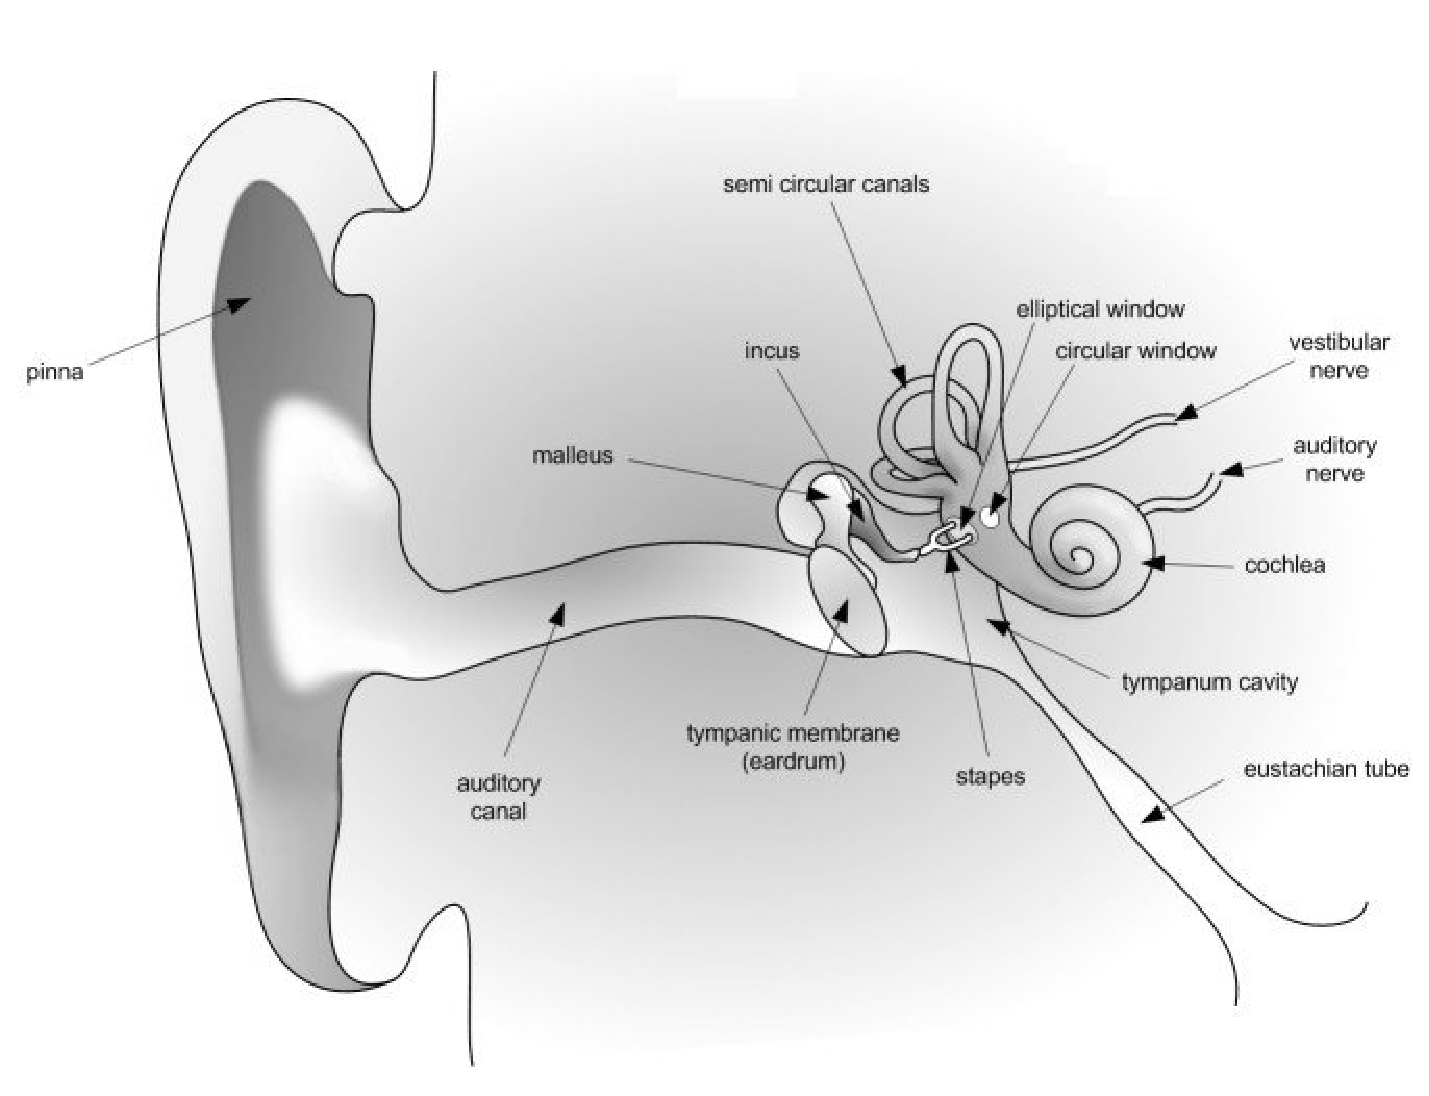
\includegraphics[width=0.65\textwidth]{../HumanEar-GrayScale.eps}
\caption{Diagram of the human ear. }
\label{Human Ear}
\end{figure}
\end{center}

The human ear is divided into three main sections: the outer, middle,
and inner ear. Let's follow the journey of a sound wave from the pinna (outermost part) to the auditory nerve (innermost part) which transmits a signal to the brain. The pinna  is the part of the ear we typically think of when we refer to the ear. Its main
function is to collect and focus an incident sound wave. The wave
then travels through the ear canal until it meets the eardrum. The
pressure fluctuations of the sound wave make the eardrum vibrate.
The three very small bones of the middle ear, the malleus (hammer),
the incus (anvil), and the stapes (stirrup), transmit the signal through
to the elliptical window. The elliptical window is the beginning of the
inner ear. From the elliptical window the sound waves are transmitted through the liquid
in the inner ear and interpreted as sounds by the brain.
The inner ear, made of the semicircular canals, the cochlea,
and the auditory nerve, is filled with fluid. The fluid allows the body to
detect quick movements and maintain balance. The snail-shaped cochlea
is covered in nerve cells. There are more than 25 000 hairlike
nerve cells. Different nerve cells vibrate with different
frequencies. When a nerve cell vibrates, it releases electrical impulses
to the auditory nerve. The impulses are sent to the brain through the
auditory nerve and understood as sound.

\subsection{Intensity of Sound}
Intensity is one indicator of amplitude. Intensity is the energy transmitted over a unit of area each second.

\Extension{Intensity}{Intensity is defined as:
\nequ{\rm{Intensity}=\frac{\rm{energy}}{\rm{time} \times \rm{area}}=\frac{\rm{power}}{\rm{area}}}

By the definition of intensity, we can see that the units of intensity are
\nequ{\frac{\rm{Joules}}{\mathrm{s \cdot m^{2}}}=\frac{\rm{Watts}}{\rm{m}^{2}}}
}

The unit of intensity is the \textbf{decibel} (symbol: dB). This reduces to an SI equivalent of $\mathrm{W \cdot m^{-2}}$.

The average threshold of hearing is $10^{-12}~\mathrm{W\cdot m^{-2}}$. Below this intensity, the sound is too soft for the ear to hear. The threshold of pain is $1.0~\mathrm{W\cdot m^{-2}}$. Above this intensity a sound is so loud it becomes uncomfortable for
the ear.

Notice that there is a factor of $10^{12}$ between the thresholds of
hearing and pain. This is one reason we define the decibel (dB) scale.

\Extension{dB Scale}{The intensity in dB of a sound of intensity $I$, is given by:
\begin{equation}
\beta =10~\log\frac{I}{I_o} \qquad \qquad {I_o}=10^{-12}~\mathrm{W\cdot m^{-2}}
\end{equation}}

In this way we can compress the whole hearing intensity scale into a
range from 0 dB to 120 dB.

\begin{table}[H]
\begin{center}
\caption{Examples of sound intensities.}
\label{p:wsl:s11:intensity}
\begin{tabular}{|l|c|c|}\hline
\textbf{Source}&\textbf{Intensity} (dB) & \textbf{Times greater than hearing threshold}\\\hline
& & \\
Rocket Launch &180 & $10^{18}$\\
Jet Plane & 140 & $10^{14}$ \\
Threshold of Pain & 120 & $10^{12}$\\
Rock Band & 110 & $10^{11}$\\
Subway Train & 90 & $10^{9}$\\
Factory & 80 & $10^{8}$\\
City Traffic & 70 & $10^{7}$\\
Normal Conversation & 60 & $10^{6}$\\
Library & 40 & $10^{4}$\\
Whisper & 20 & $10^{2}$\\
Threshold of hearing & 0 & 0\\
\hline
\end{tabular}
\end{center}
\end{table}

Notice that there are sounds which exceed the threshold
of pain. Exposure to these sounds can cause immediate damage to hearing.
In fact, exposure to sounds from
80 dB and above can damage hearing over time. Measures
can be taken to avoid damage, such as wearing earplugs
or ear muffs. Limiting exposure time and
increasing distance between you and the source are also
important steps for protecting your hearing.

\Activity{Discussion}{Importance of Safety Equipment}{Working in groups of 5, discuss the importance of safety equipment such as ear protectors for workers in loud environments, e.g. those who use jack hammers or direct aeroplanes to their parking bays. Write up your conclusions in a one page report. Some prior research into the importance of safety equipment might be necessary to complete this group discussion.}

\section{Ultrasound}
%\begin{syllabus}
%\item The learner must be able to describe sound with frequencies higher than 20 kHz as ultrasound, up to about 100 kHz.
%\item The learner must be able to explain how an image can be created using ultrasound based on the fact that when a wave encounters a boundary between two media, part of the wave is reflected and part is transmitted.
%\item The learner must be able to describe some of the medical benefits and uses of ultrasound, e.g. safety, diagnosis, treatment, pregnancy.
%\item Notes: Make a link to Grade 10, reflection and transmission at a boundary. When an ultrasound wave travels inside an object comprising different materials such as the human body, each time it encounters a boundary, e.g. between bone and muscle, or muscle and fat, part of the wave is reflected and part of it is transmitted. The reflected rays are detected and used to construct an image of the object.
%\end{syllabus}

Ultrasound is sound with a frequency that is higher than 20 kHz. Some animals, such as dogs, dolphins, and bats, have an upper limit that is greater than that of the human ear and can hear ultrasound.

The most common use of ultrasound is to create images, and has industrial and medical applications. The use of ultrasound to create images is based on the reflection and transmission of a wave at a boundary. When an ultrasound wave travels inside an object that is made up of different materials such as the human body, each time it encounters a boundary, e.g. between bone and muscle, or muscle and fat, part of the wave is reflected and part of it is transmitted. The reflected rays are detected and used to construct an image of the object.

Ultrasound in medicine can visualise muscle and soft tissue, making them useful for scanning the organs, and is commonly used during pregnancy. Ultrasound is a safe, non-invasive method of looking inside the human body.

Ultrasound sources may be used to generate local heating in biological tissue, with applications in physical therapy and cancer treatment. Focussed ultrasound sources may be used to break up kidney stones.

Ultrasonic cleaners, sometimes called supersonic cleaners, are used at frequencies from 20-40 kHz for jewellery, lenses and other optical parts, watches, dental instruments, surgical instruments and industrial parts.
These cleaners consist of containers with a fluid in which the object to be cleaned is placed. Ultrasonic waves are then sent into the fluid. The main mechanism for cleaning action in an ultrasonic cleaner is actually the energy released from the collapse of millions of microscopic bubbles occurring in the liquid of the cleaner.

\begin{IFact}{Ultrasound generator/speaker systems are sold with claims that they frighten away rodents and insects, but there is no scientific evidence that the devices work; controlled tests have shown that rodents quickly learn that the speakers are harmless.
}\end{IFact}

%\begin{IFact}
%{Medical ultrasonography was invented in 1953 at Lund University in Sweden by cardiologist Inge Edler and Carl Hellmuth %Hertz, the son of Gustav Ludwig Hertz, who was a graduate student at the department for nuclear physics.}
%\end{IFact}

%\begin{IFact}{In echo-sounding the reflections from ultrasound pulses that are bounced off objects (for example the bottom of the sea, fish etc.) are picked up. The reflections are timed and since their speed is known, the distance to the object can be found. This information can be built into a picture of the object that reflects the ultrasound pulses.}
%\end{IFact}

%In medical scanning, the ultrasound is reflected off each tissue boundary and is picked up. %The reflections are used to build up a picture showing what is inside the body, for example %in pre-natal scans. Some of the ultrasound energy is absorbed by the body, but it is much %less damaging than x-rays.

\section{SONAR}

\begin{center}
\scalebox{0.8} % Change this value to rescale the drawing.
{
\begin{pspicture}(0,-3.93)(11.42,3.91)
\definecolor{color78b}{rgb}{0.6,0.6,0.6}
\psbezier[linewidth=0.04](0.52,-1.6283582)(3.3282945,-0.05)(4.980751,-1.0964925)(5.8,-2.11)(6.619249,-3.1235075)(8.99,-3.91)(10.64,-3.71)
\psbezier[linewidth=0.04,fillstyle=solid,fillcolor=color78b](1.94,2.61)(1.9801459,1.77)(1.84,1.17)(2.44,1.15)(3.04,1.13)(6.68,1.01)(7.358321,1.29)(8.036642,1.57)(9.52,2.81)(8.58,2.59)(7.64,2.37)(1.96,2.43)(1.92,2.59)
\psline[linewidth=0.04cm](2.52,2.49)(2.52,3.27)
\psline[linewidth=0.04cm](2.52,3.27)(4.44,3.27)
\psline[linewidth=0.04cm](4.44,3.27)(4.44,2.45)
\psline[linewidth=0.04cm](3.14,3.81)(3.14,3.27)
\psline[linewidth=0.04cm](3.76,3.81)(3.76,3.27)
\psellipse[linewidth=0.04,dimen=outer](3.45,3.82)(0.33,0.09)
\pscircle[linewidth=0.04,dimen=outer,fillstyle=solid,fillcolor=color78b](2.74,3.05){0.14}
\pscircle[linewidth=0.04,dimen=outer,fillstyle=solid,fillcolor=color78b](3.18,3.05){0.14}
\pscircle[linewidth=0.04,dimen=outer,fillstyle=solid,fillcolor=color78b](3.7,3.05){0.14}
\pscircle[linewidth=0.04,dimen=outer,fillstyle=solid,fillcolor=color78b](4.12,3.05){0.14}
\pscircle[linewidth=0.04,dimen=outer,fillstyle=solid,fillcolor=color78b](2.96,2.77){0.14}
\pscircle[linewidth=0.04,dimen=outer,fillstyle=solid,fillcolor=color78b](3.44,2.77){0.14}
\pscircle[linewidth=0.04,dimen=outer,fillstyle=solid,fillcolor=color78b](3.9,2.75){0.14}
\rput(7.5798435,2.24){SAS Sonar}
\psframe[linewidth=0.04,dimen=outer,fillstyle=solid](3.24,1.15)(3.02,1.05)
\psframe[linewidth=0.04,dimen=outer,fillstyle=solid](4.58,1.13)(4.36,1.03)
\pscustom[linewidth=0.04]
{
\newpath
\moveto(9.94,1.31)
}
\psline[linewidth=0.04cm](0.0,1.61)(11.4,1.61)
\psline[linewidth=0.04cm](3.12,1.15)(3.76,-0.85)
\psline[linewidth=0.04cm](3.76,-0.85)(4.48,1.13)
\psline[linewidth=0.04cm](3.2972062,0.25496995)(3.4476187,0.11434252)
\psline[linewidth=0.04cm](3.4476187,0.11434252)(3.4875562,0.316345)
\psline[linewidth=0.04cm](4.229458,0.10226333)(4.187863,0.30393106)
\psline[linewidth=0.04cm](4.187863,0.30393106)(4.0386105,0.1620733)
\rput(3.2217188,-1.2){seabed}
\rput(1.949375,0.62){transmitter}
\rput(5.47,0.62){receiver}
\psline[linewidth=0.04cm,arrowsize=0.05291667cm 2.0,arrowlength=1.4,arrowinset=0.4]{->}(2.56,0.81)(3.0,1.03)
\psline[linewidth=0.04cm,arrowsize=0.05291667cm 2.0,arrowlength=1.4,arrowinset=0.4]{->}(4.92,0.79)(4.64,1.03)
%\psline[linewidth=0.04cm,arrowsize=0.05291667cm %2.0,arrowlength=1.4,arrowinset=0.4]{->}(6.36,-0.09)(6.36,-0.09)
\rput(7.020781,-0.46){sea}
\end{pspicture}
}
\end{center}

Ships on the ocean make use of the reflecting properties of sound waves to determine the depth of the ocean. A sound wave is transmitted and bounces off the seabed. Because the speed of sound is known and the time lapse between sending and receiving the sound can be measured, the distance from the ship to the bottom of the ocean can be determined, This is called sonar, which stands from \textbf{So}und \textbf{N}avigation \textbf{A}nd \textbf{R}anging.

\subsection{Echolocation}
Animals like dolphins and bats make use of sounds waves to find their way. Just like ships on the ocean, bats use sonar to navigate. Ultrasound waves that are sent out are reflected off the objects around the animal. Bats, or dolphins, then use the reflected sounds to form a ``picture'' of their surroundings. This is called echolocation.

\begin{wex}{SONAR}
{A ship sends a signal to the bottom of the ocean to determine the depth of the ocean. The speed of sound in sea water is 1450 $\rm{m.s^{-1}}$ If the signal is received 1,5 seconds later, how deep is the ocean at that point?}
{
\westep{Identify what is given and what is being asked:}
\begin{eqnarray*}
s &=& 1450 \ \rm{m.s^{-1}}\\
t &=& 1,5 \ \rm{s} \ \rm{there \ and \ back}\\
\therefore t &= & 0,75 \ \rm{s} \ \rm{one \ way}\\
d &=& ?
\end{eqnarray*}

\westep{Calculate the distance:}
\begin{eqnarray*}
\rm{Distance} &=& \rm{speed} \times \rm{time} \\
d &=& s \times t \\
&=& 1450 m.s^{-1} \times 0,75 s \\
&=& 1087,5 \ \rm{m}
\end{eqnarray*}

}
\end{wex}

\section{Summary}

\begin{enumerate}
\item Sound waves are longitudinal waves
\item The \textbf{frequency} of a sound is an indication of how high or low the \emph{pitch} of the sound is.
\item The human ear can hear frequencies from 20 to 20~000 Hz. \\
\textbf{Infrasound} waves have frequencies lower than 20 Hz. \\
\textbf{Ultrasound} waves have frequencies higher than 20~000 Hz.
\item The \textbf{amplitude} of a sound determines its \emph{loudness} or volume.
\item The \textbf{tone} is a measure of the \emph{quality} of a sound wave.
\item The speed of sound in air is around 340 m.s$^{-1}$. It is dependent on the temperature, height above sea level and the phase of the medium through which it is travelling.
\item Sound travels faster when the medium is hot.
\item Sound travels faster in a solid than a liquid and faster in a liquid than in a gas.
\item Sound travels faster at sea level where the air pressure is higher.
\item The intensity of a sound is the energy transmitted over a certain area. Intensity is a measure of frequency.
\item Ultrasound can be used to form pictures of things we cannot see, like unborn babies or tumors.
\item Echolocation is used by animals such as dolphins and bats to ``see'' their surroundings by using ultrasound.
\item Ships use sonar to determine how deep the ocean is or to locate shoals of fish.
\end{enumerate}

\section{Exercises}

\renewcommand{\labelenumii}{\Alph{enumii}}
\begin{enumerate}

\item Choose a word from column B that best describes the concept in column A. \\
\begin{center}
\begin{tabular}{ll}
\textbf{Column A} & \textbf{Column B} \\ \hline
pitch of sound \ \ \ & amplitude \\
loudness of sound \ \ \ \ \ \ \ \ \ & frequency \\
quality of sound \ \ \ & speed \\
& waveform \\
\end{tabular}
\end{center}

\item A tuning fork, a violin string and a loudspeaker are producing sounds. This is because they are all in a state of:
\begin{enumerate}
\item compression
\item rarefaction
\item rotation
\item tension
\item vibration
\end{enumerate}

\item What would a drummer do to make the sound of a drum give a note of lower pitch?
\begin{enumerate}
\item hit the drum harder
\item hit the drum less hard
\item hit the drum near the edge
\item loosen the drum skin
\item tighten the drum skin
\end{enumerate}

\item What is the approximate range of audible frequencies for a healthy human?
\begin{enumerate}
\item 0.2 Hz $\rightarrow$ 200 Hz
\item 2 Hz $\rightarrow$ 2 000 Hz
\item 20 Hz $\rightarrow$ 20 000 Hz
\item 200 Hz $\rightarrow$ 200 000 Hz
\item 2 000 Hz $\rightarrow$ 2 000 000 Hz
\end{enumerate}

\item X and Y are different wave motions. In air, X travels much faster than Y but has a much shorter wavelength. Which types of wave motion could X and Y be?

\begin{tabular}{lll}
& \underline{X} & \underline{Y}\\
A & microwaves & red light\\
B & radio & infra red\\
C & red light & sound\\
D & sound & ultraviolet\\
E & ultraviolet & radio\\
\end{tabular}

\item Astronauts are in a spaceship orbiting the moon. They see an explosion on the surface of the moon. Why can they not hear the explosion?
\begin{enumerate}
\item explosions do not occur in space
\item sound cannot travel through a vacuum
\item sound is reflected away from the spaceship
\item sound travels too quickly in space to affect the ear drum
\item the spaceship would be moving at a supersonic speed
\end{enumerate}

\item A man stands between two cliffs as shown in the diagram and claps his hands once.

% Generated with LaTeXDraw 1.9.3
% Tue Oct 23 18:53:18 SAST 2007
% \usepackage[usenames,dvipsnames]{pstricks}
% \usepackage{epsfig}
% \usepackage{pst-grad} % For gradients
% \usepackage{pst-plot} % For axes
%\scalebox{1} % Change this value to rescale the drawing.
\begin{center}
{
\begin{pspicture}(0,-1.0985937)(7.6665626,1.1185937)
\psline[linewidth=0.04cm](1.260625,0.92140627)(1.260625,-1.0785937)
\psline[linewidth=0.04cm](6.260625,0.94140625)(6.260625,-1.0585938)
%\usefont{T1}{ptm}{m}{n}
\rput(0.4575,0.47140625){cliff 1}
%\usefont{T1}{ptm}{m}{n}
\rput(7.1339064,0.49140626){cliff 2}
\psline[linewidth=0.04cm](1.260625,-1.0785937)(6.240625,-1.0585938)
\psline[linewidth=0.04cm](4.260625,0.88140625)(4.240625,0.52140623)
\psline[linewidth=0.04cm,arrowsize=0.1029cm 2.04,arrowlength=1.44,arrowinset=0.4]{<->}(1.240625,0.70140624)(4.240625,0.70140624)
\psline[linewidth=0.04cm,arrowsize=0.0929cm 2.05,arrowlength=1.45,arrowinset=0.4]{<->}(4.300625,0.70140624)(6.260625,0.70140624)
\pscircle[linewidth=0.04,dimen=outer](4.250625,0.21140625){0.25}
\psline[linewidth=0.04cm](4.240625,-0.05859375)(4.240625,-0.6585938)
\psline[linewidth=0.04cm](4.240625,-0.6585938)(3.940625,-1.0585938)
\psline[linewidth=0.04cm](4.240625,-0.6585938)(4.540625,-1.0585938)
\psline[linewidth=0.04cm](4.040625,-0.25859374)(4.440625,-0.25859374)
%\usefont{T1}{ptm}{m}{n}
\rput(2.6015625,0.94140625){\footnotesize 165 m}
%\usefont{T1}{ptm}{m}{n}
\rput(5.2015624,0.94140625){\footnotesize 110 m}
\end{pspicture}
}
\end{center}

Assuming that the velocity of sound is 330 m.s$^{-1}$, what will be the time interval between the two loudest echoes?
\begin{enumerate}
\item $\frac{1}{6}$ s
\item $\frac{5}{6}$ s
\item $\frac{1}{3}$ s
\item $1$ s
\item $\frac{2}{3}$ s
\end{enumerate}

\item A dolphin emits an ultrasonic wave with frequency of 0,15 MHz. The speed of the ultrasonic wave in water is 1 500 m.s$^{-1}$. What is the wavelength of this wave in water?
\begin{enumerate}
\item 0.1 mm
\item 1 cm
\item 10 cm
\item 10 m
\item 100 m
\end{enumerate}

\comment{
\item A stamp collecter is using a magnifying glass to see a stamp more clearly.
Where should the stamp be placed?

% Generated with LaTeXDraw 1.9.3
% Tue Oct 23 20:07:16 SAST 2007
% \usepackage[usenames,dvipsnames]{pstricks}
% \usepackage{epsfig}
% \usepackage{pst-grad} % For gradients
% \usepackage{pst-plot} % For axes
%\scalebox{1} % Change this value to rescale the drawing.
\begin{center}
{
\begin{pspicture}(0,-2.3428125)(11.05875,2.3228126)
\definecolor{color1683b}{rgb}{0.011764705882352941,0.027450980392156862,0.027450980392156862}
\definecolor{color2300b}{rgb}{0.03529411764705882,0.01568627450980392,0.01568627450980392}
\pspolygon[linewidth=0.04](1.26,-1.0971875)(1.26,0.44535795)(2.32,0.5828125)(2.32,-0.95973295)(2.32,-0.95973295)(2.32,-0.95973295)(2.32,-0.95973295)
\pscustom[linewidth=0.04]
{
\newpath
\moveto(4.04,2.3028126)
}
\pscustom[linewidth=0.04]
{
\newpath
\moveto(1.26,0.6028125)
\lineto(1.3,0.5928125)
\curveto(1.32,0.5878125)(1.365,0.5878125)(1.39,0.5928125)
\curveto(1.415,0.5978125)(1.455,0.6228125)(1.47,0.6428125)
\curveto(1.485,0.6628125)(1.53,0.6728125)(1.56,0.6628125)
\curveto(1.59,0.6528125)(1.645,0.6328125)(1.67,0.6228125)
\curveto(1.695,0.6128125)(1.735,0.6128125)(1.75,0.6228125)
\curveto(1.765,0.6328125)(1.8,0.6378125)(1.82,0.6328125)
\curveto(1.84,0.6278125)(1.885,0.6178125)(1.91,0.6128125)
\curveto(1.935,0.6078125)(1.975,0.6228125)(1.99,0.6428125)
\curveto(2.005,0.6628125)(2.05,0.6728125)(2.08,0.6628125)
\curveto(2.11,0.6528125)(2.165,0.6478125)(2.19,0.6528125)
\curveto(2.215,0.6578125)(2.26,0.6778125)(2.28,0.6928125)
\curveto(2.3,0.7078125)(2.355,0.7128125)(2.39,0.7028125)
\curveto(2.425,0.6928125)(2.46,0.6678125)(2.46,0.6528125)
\curveto(2.46,0.6378125)(2.445,0.5978125)(2.43,0.5728125)
\curveto(2.415,0.5478125)(2.405,0.4928125)(2.41,0.4628125)
\curveto(2.415,0.4328125)(2.43,0.3828125)(2.44,0.3628125)
\curveto(2.45,0.3428125)(2.45,0.3128125)(2.44,0.3028125)
\curveto(2.43,0.2928125)(2.42,0.2628125)(2.42,0.2428125)
\curveto(2.42,0.2228125)(2.42,0.1878125)(2.42,0.1728125)
\curveto(2.42,0.1578125)(2.42,0.1178125)(2.42,0.0928125)
\curveto(2.42,0.0678125)(2.425,0.0278125)(2.43,0.0128125)
\curveto(2.435,-0.0021875)(2.445,-0.0421875)(2.45,-0.0671875)
\curveto(2.455,-0.0921875)(2.46,-0.1221875)(2.46,-0.1271875)
\curveto(2.46,-0.1321875)(2.455,-0.1671875)(2.45,-0.1971875)
\curveto(2.445,-0.2271875)(2.425,-0.2771875)(2.41,-0.2971875)
\curveto(2.395,-0.3171875)(2.39,-0.3571875)(2.4,-0.3771875)
\curveto(2.41,-0.3971875)(2.44,-0.4221875)(2.46,-0.4271875)
\curveto(2.48,-0.4321875)(2.47,-0.4571875)(2.44,-0.4771875)
\curveto(2.41,-0.4971875)(2.39,-0.5321875)(2.4,-0.5471875)
\curveto(2.41,-0.5621875)(2.42,-0.6071875)(2.42,-0.6371875)
\curveto(2.42,-0.6671875)(2.415,-0.7121875)(2.41,-0.7271875)
\curveto(2.405,-0.7421875)(2.415,-0.7721875)(2.43,-0.7871875)
\curveto(2.445,-0.8021875)(2.445,-0.8421875)(2.43,-0.8671875)
\curveto(2.415,-0.8921875)(2.4,-0.9421875)(2.4,-0.9671875)
\curveto(2.4,-0.9921875)(2.39,-1.0321875)(2.38,-1.0471874)
\curveto(2.37,-1.0621876)(2.34,-1.0871875)(2.32,-1.0971875)
\curveto(2.3,-1.1071875)(2.25,-1.1071875)(2.22,-1.0971875)
\curveto(2.19,-1.0871875)(2.14,-1.0771875)(2.12,-1.0771875)
\curveto(2.1,-1.0771875)(2.06,-1.0871875)(2.04,-1.0971875)
\curveto(2.02,-1.1071875)(1.97,-1.1221875)(1.94,-1.1271875)
\curveto(1.91,-1.1321875)(1.855,-1.1321875)(1.83,-1.1271875)
\curveto(1.805,-1.1221875)(1.75,-1.1271875)(1.72,-1.1371875)
\curveto(1.69,-1.1471875)(1.64,-1.1671875)(1.62,-1.1771874)
\curveto(1.6,-1.1871876)(1.555,-1.1971875)(1.53,-1.1971875)
\curveto(1.505,-1.1971875)(1.455,-1.1921875)(1.43,-1.1871876)
\curveto(1.405,-1.1821876)(1.35,-1.1771874)(1.32,-1.1771874)
\curveto(1.29,-1.1771874)(1.24,-1.1821876)(1.22,-1.1871876)
\curveto(1.2,-1.1921875)(1.17,-1.1771874)(1.16,-1.1571875)
\curveto(1.15,-1.1371875)(1.145,-1.0971875)(1.15,-1.0771875)
\curveto(1.155,-1.0571876)(1.15,-1.0171875)(1.14,-0.9971875)
\curveto(1.13,-0.9771875)(1.115,-0.9221875)(1.11,-0.8871875)
\curveto(1.105,-0.8521875)(1.115,-0.7921875)(1.13,-0.7671875)
\curveto(1.145,-0.7421875)(1.16,-0.7021875)(1.16,-0.6871875)
\curveto(1.16,-0.6721875)(1.145,-0.6271875)(1.13,-0.5971875)
\curveto(1.115,-0.5671875)(1.105,-0.5171875)(1.11,-0.4971875)
\curveto(1.115,-0.4771875)(1.125,-0.4371875)(1.13,-0.4171875)
\curveto(1.135,-0.3971875)(1.135,-0.3571875)(1.13,-0.3371875)
\curveto(1.125,-0.3171875)(1.12,-0.2821875)(1.12,-0.2671875)
\curveto(1.12,-0.2521875)(1.13,-0.2171875)(1.14,-0.1971875)
\curveto(1.15,-0.1771875)(1.16,-0.1321875)(1.16,-0.1071875)
\curveto(1.16,-0.0821875)(1.145,-0.0371875)(1.13,-0.0171875)
\curveto(1.115,0.0028125)(1.11,0.0628125)(1.12,0.1028125)
\curveto(1.13,0.1428125)(1.14,0.2078125)(1.14,0.2328125)
\curveto(1.14,0.2578125)(1.135,0.3078125)(1.13,0.3328125)
\curveto(1.125,0.3578125)(1.13,0.3978125)(1.14,0.4128125)
\curveto(1.15,0.4278125)(1.16,0.4678125)(1.16,0.4928125)
\curveto(1.16,0.5178125)(1.145,0.5678125)(1.13,0.5928125)
\curveto(1.115,0.6178125)(1.125,0.6428125)(1.15,0.6428125)
\curveto(1.175,0.6428125)(1.22,0.6278125)(1.24,0.6128125)
\curveto(1.26,0.5978125)(1.305,0.5528125)(1.38,0.4628125)
}
\pscircle[linewidth=0.04,dimen=outer](1.7636944,0.079230234){0.14358246}
\psline[linewidth=0.04cm](1.7606715,-0.029914629)(1.7807275,-0.452642)
\psline[linewidth=0.04cm](1.7807275,-0.43900564)(2.041455,-0.6571875)
\psline[linewidth=0.04cm](1.7807275,-0.43900564)(1.52,-0.6571875)
\psline[linewidth=0.04cm](1.5601119,-0.2071874)(2.041455,-0.19355103)
\psline[linewidth=0.04cm](0.0,-0.7771875)(8.94,-0.8171875)
\psframe[linewidth=0.04,dimen=outer,fillstyle=solid,fillcolor=color1683b](6.04,-0.9771875)(5.86,-1.5571876)
\psline[linewidth=0.05cm,linestyle=dashed,dash=0.16cm 0.16cm](4.84,1.2028126)(4.86,-0.8371875)
\psellipse[linewidth=0.04,dimen=outer](5.95,-0.3371875)(0.23,0.74)
\psline[linewidth=0.05cm,linestyle=dashed,dash=0.16cm 0.16cm](5.94,1.2028126)(5.96,-1.2571875)
\psline[linewidth=0.05cm,linestyle=dashed,dash=0.16cm 0.16cm](7.06,1.2028126)(7.08,-0.8371875)
\psdots[dotsize=0.2](4.86,-0.8171875)
\psdots[dotsize=0.2](5.4,-0.8171875)
\psdots[dotsize=0.2](4.32,-0.8171875)
\psdots[dotsize=0.2](6.5,-0.7971875)
\psdots[dotsize=0.2](7.1,-0.7971875)
%\usefont{T1}{ptm}{m}{n}
\rput(4.3071876,-1.1171875){\footnotesize A}
%\usefont{T1}{ptm}{m}{n}
\rput(4.8304687,-1.1171875){\footnotesize B}
%\usefont{T1}{ptm}{m}{n}
\rput(5.39375,-1.1171875){\footnotesize C}
%\usefont{T1}{ptm}{m}{n}
\rput(6.476719,-1.1171875){\footnotesize D}
%\usefont{T1}{ptm}{m}{n}
\rput(7.047969,-1.1171875){\footnotesize E}
\psline[linewidth=0.04cm,arrowsize=0.0929cm 2.04,arrowlength=1.44,arrowinset=0.4]{<->}(6.0,0.8828125)(7.0,0.8828125)
\psline[linewidth=0.04cm,arrowsize=0.0929cm 2.04,arrowlength=1.44,arrowinset=0.4]{<->}(4.88,0.8828125)(5.94,0.8828125)
%\usefont{T1}{ptm}{m}{n}
\rput(5.3745313,1.6428125){\footnotesize focal}
%\usefont{T1}{ptm}{m}{n}
\rput(5.389375,1.3428125){\footnotesize length}
%\usefont{T1}{ptm}{m}{n}
\rput(6.494531,1.6428125){\footnotesize focal}
%\usefont{T1}{ptm}{m}{n}
\rput(6.509375,1.3428125){\footnotesize length}
%\usefont{T1}{ptm}{m}{n}
\rput(5.969844,-1.8171875){\footnotesize magnifying}
%\usefont{T1}{ptm}{m}{n}
\rput(5.940625,-2.1371875){\footnotesize glass}
%\usefont{T1}{ptm}{m}{n}
\rput(1.7725,1.3228126){\footnotesize image}
%\usefont{T1}{ptm}{m}{n}
\rput(1.7932812,1.0028125){\footnotesize of stamp}
\rput{90.05646}(5.975181,-11.089099){\psarc[linewidth=0.04](8.526679,-2.5599015){0.91}{0.0}{52.853313}}
\rput{181.13571}(18.02571,-1.5802013){\psarc[linewidth=0.04](9.005023,-0.8794292){0.91}{0.0}{56.68937}}
\rput{90.05646}(7.074716,-10.407138){\psarc[linewidth=0.04](8.735802,-1.6696949){0.74}{50.52754}{100.30485}}
\rput{74.54539}(4.459055,-8.881291){\psellipse[linewidth=0.04,dimen=outer,fillstyle=solid,fillcolor=color2300b](8.064475,-1.5110774)(0.2013951,0.087453164)}
%\usefont{T1}{ptm}{m}{n}
\rput(9.687031,-1.0771875){\footnotesize stamp collector's}
%\usefont{T1}{ptm}{m}{n}
\rput(9.039219,-1.4171875){\footnotesize eye}
\end{pspicture}
}
\end{center}
}
\item The amplitude and frequency of a sound wave are both increased. How are the loudness and pitch of the sound affected?

\begin{tabular}{lll}
& \underline{loudness} & \underline{pitch}\\
A & increased & raised\\
B & increased & unchanged\\
C & increased & lowered\\
D & decreased & raised\\
E & decreased & lowered\\
\end{tabular}

\item A jet fighter travels slower than the speed of sound. Its speed is said to be:
\begin{enumerate}
\item Mach 1
\item supersonic
\item isosonic
\item hypersonic
\item infrasonic
\end{enumerate}

\item A sound wave is different from a light wave in that a sound wave is:
\begin{enumerate}
\item produced by a vibrating object and a light wave is not.
\item not capable of travelling through a vacuum.
\item not capable of diffracting and a light wave is.
\item capable of existing with a variety of frequencies and a light wave has a single frequency.
\end{enumerate}

\item At the same temperature, sound waves have the fastest speed in:
\begin{enumerate}
\item{rock}
\item{milk}
\item{oxygen}
\item{sand}
\end{enumerate}

\item Two sound waves are traveling through a container of nitrogen gas. The first wave has a wavelength of 1,5~m, while the second wave has a wavelength of 4,5~m. The velocity of the second wave must be:
\begin{enumerate}
\item{$\frac{1}{9}$ the velocity of the first wave.}
\item{$\frac{1}{3}$ the velocity of the first wave.}
\item{the same as the velocity of the first wave.}
\item{three times larger than the velocity of the first wave.}
\item{nine times larger than the velocity of the first wave.}
\end{enumerate}
%\end{enumerate}

\renewcommand{\labelenumii}{(\alph{enumii})}

\item{Sound travels at a speed of 340~\ms. A straw is 0,25 m long. The standing wave set up in such a straw with one end closed has a wavelength of 1,0~m. The standing wave set up in such a straw with both ends open has a wavelength of 0,50 m.
\begin{enumerate}
\item calculate the frequency of the sound created when you blow across the straw with the bottom end closed.
\item calculate the frequency of the sound created when you blow across the straw with the bottom end open.
\end{enumerate}}
\item{A lightning storm creates both lightning and thunder. You see the lightning almost immediately since light travels at $3\times10^{8}\ems$. After seeing the lightning, you count 5~s and then you hear the thunder. Calculate the distance to the location of the storm.}
\item{A person is yelling from a second story window to another person standing at the garden gate, 50~m away. If the speed of sound is 344~\ms, how long does it take the sound to reach the person standing at the gate?}
\item{A piece of equipment has a warning label on it that says, "Caution! This instrument produces 140 decibels." What safety precaution should you take before you turn on the instrument?}
\item{What property of sound is a measure of the amount of energy carried by a sound wave?}
\item{How is intensity related to loudness?}
\item Person 1 speaks to person 2. Explain how the sound is created by person 1 and how it is possible for person 2 to hear the conversation.
\item{Sound cannot travel in space. Discuss what other modes of communication astronauts can use when they are outside the space shuttle?}
\item{An automatic focus camera uses an ultrasonic sound wave to focus on objects. The camera sends out sound waves which are reflected off distant objects and return to the camera. A sensor detects the time it takes for the waves to return and then determines the distance an object is from the camera. If a sound wave (speed = 344~\ms) returns to the camera 0,150~s after leaving the camera, how far away is the object?}
\item{Calculate the frequency (in Hz) and wavelength of the annoying sound made by a mosquito when it beats its wings at the average rate of 600 wing beats per second. Assume the speed of the sound waves is 344~\ms.}
\item{How does halving the frequency of a wave source affect the speed of the waves?}
\item{Humans can detect frequencies as high as 20~000 Hz. Assuming the speed of sound in air is 344~\ms, calculate the wavelength of the sound corresponding to the upper range of audible hearing.}
\item{An elephant trumpets at 10~Hz. Assuming the speed of sound in air is 344~\ms, calculate the wavelength of this infrasonic sound wave made by the elephant.}

\item A ship sends a signal out to determine the depth of the ocean. The signal returns 2,5 seconds later. If sound travels at
1450 m.s$^{-1}$ in sea water, how deep is the ocean at that point?

\end{enumerate}


% CHILD SECTION END 



% CHILD SECTION START 

\chapter{The Physics of Music - Grade 11}
\label{p:wsl:pm11}


\section{Introduction}
What is your favorite musical instrument? How do you play it? Do you pluck a string, like a guitar? 
Do you blow through it, like a flute? Do you hit it, like a drum? 
All musical instruments work by making standing waves. Each instrument has a unique sound because of the special waves made in it. 
These waves could be in the strings of a guitar or violin. 
They could also be in the skin of a drum or a tube of air in a trumpet.  
These waves are picked up by the air and later reach your ear as sound.

In Grade 10, you learned about standing waves and boundary conditions. We saw a rope that was:
\begin{itemize}
\item{fixed at both ends}
\item{fixed at one end and free at the other}
\end{itemize}



We also saw a pipe that was:
\begin{itemize}
\item{closed at both ends}
\item{open at both ends}
\item{open at one end, closed at the other}
\end{itemize}

String and wind instruments are good examples of standing waves on strings and pipes.

One way to describe standing waves is to count nodes. 
Recall that a node is a point on a string that does not move as the wave changes. 
The anti-nodes are the highest and lowest points on the wave. There is a node at each end of a fixed string. 
There is also a node at the closed end of a pipe. 
But an open end of a pipe has an anti-node.

What causes a standing wave? There are incident and reflected waves traveling back and forth on our string or pipe. 
For some frequencies, these waves combine in just the right way so that the whole wave appears to be standing still. 
These special cases are called harmonic frequencies, or \textbf{harmonics}. 
They depend on the length and material of the medium.

\Definition{Harmonic}{A \textbf{harmonic} frequency is a frequency at which standing waves can be made in a particular object or on a particular instrument.}

\section{Standing Waves in String Instruments}
Let us look at a basic "instrument": a string pulled tight and fixed at both ends. 
When you pluck the string, you hear a certain pitch. This pitch is made by a certain frequency. 
What causes the string to emit sounds at this pitch?

You have learned that the frequency of a standing wave depends on the length of the wave. 
The wavelength depends on the nodes and anti-nodes.  
The longest wave that can "fit" on the string is shown in Figure~\ref{fig:harmonics}. 
This is called the \textbf{fundamental} or \textbf{natural frequency} of the string. 
The string has nodes at both ends. The wavelength of the fundamental is twice the length of the string.

Now put your finger on the center of the string.  Hold it down gently and pluck it. 
The standing wave now has a node in the middle of the string.  There are three nodes. 
We can fit a whole wave between the ends of the string. 
This means the wavelength is equal to the length of the string.  
This wave is called the first harmonic.  
As we add more nodes, we find the second harmonic, third harmonic, and so on.  
We must keep the nodes equally spaced or we will lose our standing wave.

\begin{figure}[htbp]
\begin{center}
\begin{pspicture}(0,-0.8)(3.6,6)
%\psgrid[gridcolor=gray]
\rput(0,4.8){\psplot[xunit=0.0111,plotstyle=curve]{0}{360}{0.5 x
mul sin} 
\psplot[xunit=0.0111,plotstyle=curve]{0}{360}{0.5 x mul sin neg}
\psline[linecolor=lightgray,linestyle=dashed](0,0)(4,0)
\uput[r](4,0){fundamental frequency}}
\rput(0,2.6){\psplot[xunit=0.0111,plotstyle=curve]{0}{360}{x
sin}\psplot[xunit=0.0111,plotstyle=curve]{0}{360}{x sin neg}
\psline[linecolor=lightgray,linestyle=dashed](0,0)(4,0)
\uput[r](4,0){first harmonic}}
\rput(0,0.4){\psplot[xunit=0.0111,plotstyle=curve]{0}{360}{1.5 x mul
sin}\psplot[xunit=0.0111,plotstyle=curve]{0}{360}{1.5 x mul sin
neg}
\psline[linecolor=lightgray,linestyle=dashed](0,0)(4,0)
\uput[r](4,0){second harmonic}}
\end{pspicture}
\caption{Harmonics on a string fixed at both ends.}
\label{fig:harmonics}
\end{center}
\end{figure}

\Activity{Investigation}{Waves on a String Fixed at Both Ends}{This chart shows various waves on a string. The string length $L$ is the dashed line. \\
\begin{enumerate}
\item{Fill in the:
\begin{itemize}
\item{number of nodes}
\item{number of anti-nodes}
\item{wavelength in terms of $L$}
\end{itemize}
The first and last waves are done for you.
\begin{center}
\begin{tabular}{|c|c|c|c|} \hline
Wave & Nodes & Antinodes & Wavelength \\ \hline
\begin{pspicture}(0,-0.6)(2,0.6)
\psline[linecolor=lightgray, linestyle=dashed](0,0)(2,0)
\scalebox{0.5}{
\psplot[xunit=0.0111,plotstyle=curve]{0}{360}{0.5 x mul sin neg}
\psplot[xunit=0.0111,plotstyle=curve]{0}{360}{0.5 x mul sin}	}
\end{pspicture}	& 
\begin{pspicture}(-1,-0.6)(1,0.6)
\rput(0,0){2}	% All this to center text!
\end{pspicture}  & 
\begin{pspicture}(-1,-0.6)(1,0.6)
\rput(0,0){1}	% All this to center text!
\end{pspicture}  & 
\begin{pspicture}(-1,-0.6)(1,0.6)
\rput(0,0){2$L$}% All this to center text!
\end{pspicture}   \\ \hline
\begin{pspicture}(0,-0.6)(2,0.6)
\psline[linecolor=lightgray, linestyle=dashed](0,0)(2,0)
\scalebox{0.5}{
\psplot[xunit=0.0111,plotstyle=curve]{0}{360}{x sin neg}
\psplot[xunit=0.0111,plotstyle=curve]{0}{360}{x sin}
}
\end{pspicture} & & & \\ \hline
\begin{pspicture}(0,-0.6)(2,0.6)
\psline[linecolor=lightgray, linestyle=dashed](0,0)(2,0)
\scalebox{0.5}{
\psplot[xunit=0.0111,plotstyle=curve]{0}{360}{1.5 x mul sin neg}
\psplot[xunit=0.0111,plotstyle=curve]{0}{360}{1.5 x mul sin}
}
\end{pspicture} & & & \\ \hline
\begin{pspicture}(0,-0.6)(2,0.6)
\psline[linecolor=lightgray, linestyle=dashed](0,0)(2,0)
\scalebox{0.5}{
\psplot[xunit=0.0111,plotstyle=curve]{0}{360}{2 x mul sin neg}
\psplot[xunit=0.0111,plotstyle=curve]{0}{360}{2 x mul sin}	}
\end{pspicture}	& 
\begin{pspicture}(-1,-0.6)(1,0.6)
\rput(0,0){5}	% All this to center text!
\end{pspicture}  & 
\begin{pspicture}(-1,-0.6)(1,0.6)
\rput(0,0){4}	% All this to center text!
\end{pspicture}  & 
\begin{pspicture}(-1,-0.6)(1,0.6)
\rput(0,0){$\frac{L}{2}$}% All this to center text!
\end{pspicture} \\ \hline
\end{tabular}
\end{center}
}
\item{Use the chart to find a formula for the wavelength in terms of the number of nodes.} \\
\end{enumerate}
}

You should have found this formula:
\nequ{\lambda=\frac{2L}{n-1}}
Here, $n$ is the number of nodes.  $L$ is the length of the
string. The frequency $f$ is:

\nequ{f=\frac{v}{\lambda}}
Here, $v$ is the velocity of the wave. This may seem confusing. 
The wave is a \emph{standing} wave, so how can it have a velocity? 
But one standing wave is made up of many waves that travel back and forth on the string. 
Each of these waves has the same velocity. This speed depends on the mass and tension of the string.

\begin{wex}
{Harmonics on a String}
{We have a standing wave on a string that is 65 cm long. The wave has a velocity of 143 m.s$^{-1}$.  
Find the frequencies of the fundamental, first, second, and third harmonics.}
{
\westep{Identify what is given and what is asked:}
\begin{eqnarray*}
\rm{L} &=& 65 \ \rm{cm} = 0.65 \ \rm{m} \\
v &=& 143 \ \rm{m.s}^{-1} \\
f &=& ?
\end{eqnarray*}
To find the frequency we will use $f = \frac{v}{\lambda}$ \\

\westep{Find the wavelength for each harmonic:}
To find $f$ we need the wavelength of each harmonic ($\lambda = \frac{2L}{n-1}$).
The wavelength is then substituted into $f = \frac{v}{\lambda}$ to find the harmonics. 
The table below shows the calculations.

\begin{center}
%\begin{tabular}{|c|p{0.5cm}|p{0.5cm}|p{0.5cm}|}\hline
\begin{tabular}{|l|c|c|c|} \hline
\begin{tabular}{c} \ \\ \ \\ \end{tabular} & \textbf{Nodes} & \begin{tabular}{c}\textbf{Wavelength} \\ $\lambda = \frac{2L}{n-1}$ \end{tabular} & \begin{tabular}{c}\textbf{Frequency}\\$f = \frac{v}{\lambda}$ \end{tabular} \\ \hline
Fundamental frequency $f_{o}$ & 2 & $\frac{2(0,65)}{2-1}$ = 1,3 & $\frac{143}{1,3}$ = 110 Hz \\\hline
First harmonic $f_{1}$ & 3 & $\frac{2(0,65)}{3-1} = 0,65 $ \ \ \  & $\frac{143}{0,65}$ = 220 Hz \\\hline
Second harmonic $f_{2}$ & 4 & $\frac{2(0,65)}{4-1} = 0,43 $ \ \ \ & $\frac{143}{0,43} = 330$ Hz  \\\hline
Third harmonic $f_{3}$ & 5 & $\frac{2(0,65)}{5-1} = 0,33 $ \ \ \ & $\frac{143}{0,33} = 440$ Hz  \\\hline
\end{tabular}
\end{center}


110 Hz is the natural frequency of the A string on a guitar. 
The third harmonic, at 440 Hz, is the note that orchestras use for tuning.}
\end{wex}

\Extension{Guitar}{Guitars use strings with high tension. 
The length, tension and mass of the strings affect the pitches you hear. 
High tension and short strings make high frequencies; low tension and long strings make low frequencies. 
When a string is first plucked, it vibrates at many frequencies. 
All of these except the harmonics are quickly filtered out. The harmonics make up the tone we hear.

The body of a guitar acts as a large wooden soundboard. Here is how a soundboard works: 
the body picks up the vibrations of the strings. It then passes these vibrations to the air. 
A sound hole allows the soundboard of the guitar to vibrate more freely. 
It also helps sound waves to get out of the body.

The neck of the guitar has thin metal bumps on it called frets.  
Pressing a string against a fret shortens the length of that string. 
This raises the natural frequency and the pitch of that string.

Most guitars use an "equal tempered" tuning of 12 notes per octave. 
A 6 string guitar has a range of 4 $\frac{1}{2}$ octaves with pitches from 82.407 Hz (low E) 
to 2093 kHz (high C). Harmonics may reach over 20 kHz, in the inaudible range.
\begin{center}
\scalebox{0.8} % Change this value to rescale the drawing. 
{ 
\begin{pspicture}(0,-3.876816)(9.885938,3.876816) \definecolor{color377b}{rgb}{0.08627450,0.04705882,0.04705882} \psline[linewidth=0.02cm,fillcolor=color377b,doubleline=true,doublesep=0.02](4.18,2.9568162)(4.48,2.796816) \psline[linewidth=0.02cm,fillcolor=color377b,doubleline=true,doublesep=0.02](3.92,2.4768162)(4.22,2.316816) \psline[linewidth=0.02cm,fillcolor=color377b,doubleline=true,doublesep=0.02](3.78,2.2368162)(4.08,2.076816) \psline[linewidth=0.02cm,fillcolor=color377b,doubleline=true,doublesep=0.02](3.64,1.9968162)(3.94,1.8368161) \psline[linewidth=0.02cm,fillcolor=color377b,doubleline=true,doublesep=0.02](3.52,1.7768161)(3.82,1.616816) \psline[linewidth=0.02cm,fillcolor=color377b,doubleline=true,doublesep=0.02](3.4,1.5368161)(3.7,1.3768162) \psline[linewidth=0.02cm,fillcolor=color377b,doubleline=true,doublesep=0.02](3.26,1.3168161)(3.56,1.1568161) \psline[linewidth=0.02cm,fillcolor=color377b,doubleline=true,doublesep=0.02](3.16,1.0968161)(3.46,0.9368161) \psline[linewidth=0.02cm,fillcolor=color377b,doubleline=true,doublesep=0.02](3.0,0.8968161)(3.3,0.7368161) \psline[linewidth=0.02cm,fillcolor=color377b,doubleline=true,doublesep=0.02](2.9,0.6568161)(3.2,0.4968161) \psline[linewidth=0.02cm,fillcolor=color377b,doubleline=true,doublesep=0.02](2.78,0.4768161)(3.08,0.3168161) \psline[linewidth=0.02cm,fillcolor=color377b,doubleline=true,doublesep=0.02](2.68,0.2768161)(2.98,0.1168161) \psline[linewidth=0.02cm,fillcolor=color377b,doubleline=true,doublesep=0.02](2.58,0.0968161)(2.88,-0.06318389) \psline[linewidth=0.02cm,fillcolor=color377b,doubleline=true,doublesep=0.02](2.48,-0.0431839)(2.78,-0.2031839) \psline[linewidth=0.02cm,fillcolor=color377b,doubleline=true,doublesep=0.02](2.42,-0.1631839)(2.72,-0.3231839) \psline[linewidth=0.02cm,fillcolor=color377b,doubleline=true,doublesep=0.02](2.36,-0.2631839)(2.66,-0.4231839) \psline[linewidth=0.02cm,fillcolor=color377b,doubleline=true,doublesep=0.02](4.04,2.7368162)(4.38,2.5368161) \psline[linewidth=0.02cm,fillcolor=color377b,doubleline=true,doublesep=0.02](4.28,3.156816)(4.62,2.9768162) \psbezier[linewidth=0.04](2.74,0.4968161)(2.5,0.6368161)(2.14,0.6968161)(1.8,0.3768161)(1.46,0.0568161)(1.5412558,-0.5595761)(1.34,-0.8831839)(1.1387441,-1.2067916)(1.1,-0.9631839)(0.56,-1.4031839)(0.02,-1.8431839)(0.11526374,-2.7895515)(0.96,-3.323184)(1.8047363,-3.8568163)(2.8687515,-3.3244164)(2.86,-2.5031838)(2.8512485,-1.6819514)(2.76,-1.7831839)(2.88,-1.4831839)(3.0,-1.1831839)(3.58,-0.6631839)(3.58,-0.3431839)(3.58,-0.02318389)(3.36,0.2768161)(3.14,0.3168161) \psbezier[linewidth=0.04,fillcolor=color377b](1.34,-3.4831839)(1.7,-3.683184)(2.7,-3.683184)(3.0,-3.0231838)(3.3,-2.363184)(2.9,-2.123184)(3.08,-1.6231838)(3.26,-1.1231838)(3.68,-0.8631839)(3.74,-0.6031839)(3.8,-0.3431839)(3.76,0.07681610)(3.2,0.2968161) \rput{-26.990808}(0.6111867,0.94451004){\psellipse[linewidth=0.04,dimen=outer,fillstyle=solid,fillcolor=color377b](2.2733724,-0.8010828)(0.25262824,0.3639826)} \rput{-210.56396}(3.8130887,-2.6515872){\psellipse[linewidth=0.04,dimen=outer](2.2687922,-0.80486655)(0.3635264,0.51368535)} \rput{-25.358118}(1.1215806,0.3934178){\psframe[linewidth=0.04,dimen=outer](1.9092686,-2.203509)(0.9610243,-2.388414)} \rput{-29.524796}(-0.17041595,1.8490239){\psframe[linewidth=0.04,dimen=outer](3.6416314,3.4273822)(3.2048702,-0.9316416)} \pscustom[linewidth=0.04] { \newpath \moveto(3.26,0.5368161) \lineto(3.25,0.4868161) \curveto(3.245,0.4618161)(3.245,0.4118161)(3.25,0.3868161) \curveto(3.255,0.3618161)(3.275,0.3218161)(3.29,0.3068161) \curveto(3.305,0.29181612)(3.32,0.2718161)(3.32,0.2568161) } \psline[linewidth=0.04cm,fillcolor=color377b](4.66,3.0168161)(2.5,-0.8231839) \psline[linewidth=0.04cm,fillcolor=color377b](4.34,3.2168162)(4.68,3.856816) \psline[linewidth=0.04cm,fillcolor=color377b](5.0,3.7368162)(5.16,3.576816) \psline[linewidth=0.04cm,fillcolor=color377b](5.16,3.576816)(4.82,3.076816) \psline[linewidth=0.04cm,fillcolor=color377b](5.18,3.596816)(4.78,3.116816) \psline[linewidth=0.04cm,fillcolor=color377b](5.14,3.576816)(4.76,3.076816) \pscustom[linewidth=0.04] { \newpath \moveto(4.64,3.0368161) \lineto(4.71,3.076816) \curveto(4.745,3.096816)(4.785,3.116816)(4.8,3.116816) } \pscustom[linewidth=0.04] { \newpath \moveto(4.68,3.056816) \lineto(4.74,3.056816) \curveto(4.77,3.056816)(4.795,3.0618162)(4.79,3.066816) \curveto(4.785,3.0718162)(4.775,3.076816)(4.77,3.076816) \curveto(4.765,3.076816)(4.77,3.0918162)(4.78,3.106816) } \pscustom[linewidth=0.04] { \newpath \moveto(4.68,3.856816) \lineto(4.75,3.856816) \curveto(4.785,3.856816)(4.825,3.8418162)(4.83,3.826816) \curveto(4.835,3.8118162)(4.835,3.796816)(4.83,3.796816) \curveto(4.825,3.796816)(4.835,3.796816)(4.85,3.796816) \curveto(4.865,3.796816)(4.9,3.801816)(4.92,3.806816) \curveto(4.94,3.8118162)(4.97,3.801816)(4.98,3.7868161) \curveto(4.99,3.771816)(5.0,3.7468162)(5.0,3.7168162) } \psellipse[linewidth=0.04,dimen=outer](5.01,3.2268162)(0.07,0.09) \psellipse[linewidth=0.04,dimen=outer](4.89,3.086816)(0.07,0.09) \pscustom[linewidth=0.04] { \newpath \moveto(4.58,3.7568161) \lineto(4.56,3.7268162) \curveto(4.55,3.711816)(4.545,3.681816)(4.55,3.666816) \curveto(4.555,3.6518161)(4.55,3.636816)(4.52,3.636816) } \pscustom[linewidth=0.04] { \newpath \moveto(4.5,3.596816) \lineto(4.46,3.566816) \curveto(4.44,3.551816)(4.425,3.5168161)(4.43,3.4968162) \curveto(4.435,3.4768162)(4.44,3.451816)(4.44,3.4368162) } \pscustom[linewidth=0.04] { \newpath \moveto(4.36,3.396816) \lineto(4.33,3.356816) \curveto(4.315,3.336816)(4.315,3.306816)(4.33,3.296816) \curveto(4.345,3.2868161)(4.36,3.271816)(4.36,3.2568161) } \psline[linewidth=0.02cm,fillcolor=color377b,doubleline=true,doublesep=0.04](5.06,3.4368162)(4.6,3.676816) \psline[linewidth=0.06cm,fillcolor=color377b](4.96,3.616816)(4.6,3.136816) \psline[linewidth=0.06cm,fillcolor=color377b](4.78,3.7168162)(4.5,3.2168162) \psline[linewidth=0.02cm,fillcolor=color377b,doubleline=true,doublesep=0.04](4.82,3.136816)(4.4,3.356816) \psline[linewidth=0.02cm,fillcolor=color377b,doubleline=true,doublesep=0.04](4.9,3.296816)(4.5,3.4968162) \psline[linewidth=0.02cm,fillcolor=color377b,doubleline=true,doublesep=0.04](1.7,-2.403184)(1.12,-2.143184) \psline[linewidth=0.02cm,fillcolor=color377b](4.36,3.156816)(1.26,-2.2431839) \psline[linewidth=0.02cm,fillcolor=color377b](4.42,3.156816)(1.32,-2.2831838) \psline[linewidth=0.02cm,fillcolor=color377b](4.44,3.136816)(1.38,-2.2831838) \psline[linewidth=0.02cm,fillcolor=color377b](4.5,3.096816)(1.44,-2.3031838) \psline[linewidth=0.02cm,fillcolor=color377b](4.56,3.096816)(1.48,-2.343184) \psline[linewidth=0.02cm,fillcolor=color377b](4.62,3.096816)(1.54,-2.363184) \psline[linewidth=0.02cm,fillcolor=color377b](4.38,3.1968162)(4.66,3.656816) \psline[linewidth=0.02cm,fillcolor=color377b](4.42,3.176816)(4.6,3.4768162) \psline[linewidth=0.02cm,fillcolor=color377b](4.46,3.156816)(4.56,3.316816) \psline[linewidth=0.02cm,fillcolor=color377b](4.5,3.136816)(4.6,3.2768161) \psline[linewidth=0.02cm,fillcolor=color377b](4.54,3.096816)(4.74,3.396816) \psline[linewidth=0.02cm,fillcolor=color377b](4.6,3.076816)(4.96,3.4968162) \psdots[dotsize=0.06](1.24,-2.2231839) \psdots[dotsize=0.06](1.32,-2.2631838) \psdots[dotsize=0.06](1.4,-2.2831838) \psdots[dotsize=0.06](1.42,-2.343184) \psdots[dotsize=0.06](1.48,-2.343184) \psdots[dotsize=0.06](1.54,-2.363184) \psdots[dotsize=0.06](1.26,-2.2231839) \psellipse[linewidth=0.04,dimen=outer](5.11,3.406816)(0.07,0.09) \psline[linewidth=0.02cm,fillcolor=color377b,arrowsize=0.05291667cm 5.1,arrowlength=1.4,arrowinset=0.4]{<-}(5.16,3.576816)(6.2,3.576816) \psline[linewidth=0.02cm,fillcolor=color377b,arrowsize=0.05291667cm 5.1,arrowlength=1.4,arrowinset=0.4]{<-}(4.96,3.056816)(6.2,3.056816) \psline[linewidth=0.02cm,fillcolor=color377b,arrowsize=0.05291667cm 5.1,arrowlength=1.4,arrowinset=0.4]{<-}(4.14,2.056816)(6.22,2.056816) \psline[linewidth=0.02cm,fillcolor=color377b,arrowsize=0.05291667cm 5.1,arrowlength=1.4,arrowinset=0.4]{<-}(3.82,1.476816)(6.2,1.476816) \psline[linewidth=0.02cm,fillcolor=color377b,arrowsize=0.05291667cm 5.1,arrowlength=1.4,arrowinset=0.4]{<-}(3.28,0.3768161)(6.22,0.3768161) \psline[linewidth=0.02cm,fillcolor=color377b,arrowsize=0.05291667cm 5.1,arrowlength=1.4,arrowinset=0.4]{<-}(3.78,-0.4231839)(6.22,-0.4431839) \psline[linewidth=0.02cm,fillcolor=color377b,arrowsize=0.05291667cm 5.1,arrowlength=1.4,arrowinset=0.4]{<-}(2.62,-0.9231839)(6.2,-0.9231839) \psline[linewidth=0.02cm,fillcolor=color377b,arrowsize=0.05291667cm 5.1,arrowlength=1.4,arrowinset=0.4]{<-}(2.34,-1.9231839)(6.2,-1.9231839) \psline[linewidth=0.02cm,fillcolor=color377b,arrowsize=0.05291667cm 5.1,arrowlength=1.4,arrowinset=0.4]{<-}(1.9,-2.423184)(6.22,-2.423184) 
%\usefont{T1}{ptm}{m}{n} 
\rput(7.124375,3.586816){headstock} 
%\usefont{T1}{ptm}{m}{n} 
\rput(6.5485935,3.086816){peg} 
%\usefont{T1}{ptm}{m}{n} 
\rput(6.5532813,2.086816){fret} 
%\usefont{T1}{ptm}{m}{n} 
\rput(6.644375,1.486816){neck} 
%\usefont{T1}{ptm}{m}{n} 
\rput(6.5873437,0.3868161){heel} 
%\usefont{T1}{ptm}{m}{n} 
\rput(6.46625,-0.4131839){rib} 
%\usefont{T1}{ptm}{m}{n} 
\rput(6.8403125,-0.9131839){rosette} 
%\usefont{T1}{ptm}{m}{n} 
\rput(8.035625,-1.9331839){hollow wooden body} 
%\usefont{T1}{ptm}{m}{n} 
\rput(6.7803125,-2.413184){bridge} 
\end{pspicture} 
}
\end{center}
}

\Extension{Piano}{Let us look at another stringed instrument: the piano. 
The piano has strings that you cannot see. When a key is pressed, a felt-tipped hammer hits a 
string inside the piano. The pitch depends on the length, tension and mass of the string. 
But there are many more strings than keys on a piano. This is because the short and thin 
strings are not as loud as the long and heavy strings.  To make up for this, the higher 
keys have groups of two to four strings each.

The soundboard in a piano is a large cast iron plate. It picks up vibrations 
from the strings. This heavy plate can withstand over 200 tons of pressure from string tension! 
Its mass also allows the piano to sustain notes for long periods
of time.
	
The piano has a wide frequency range, from 27,5 Hz (low A) to 4186,0 Hz 
(upper C). But these are just the fundamental frequencies. A piano plays complex, 
rich tones with over 20 harmonics per note. Some of these are out of the range of human hearing. 
Very low piano notes can be heard mostly because of their higher harmonics.

\begin{center}
\scalebox{1} % Change this value to rescale the drawing.
{
\begin{pspicture}(0,-3.7196875)(9.475264,3.6896875)
\definecolor{color377b}{rgb}{0.08627450,0.04705882,0.04705882}
\psline[linewidth=0.02cm,fillcolor=color377b](1.41,3.6796875)(0.43,3.1796875)
\psline[linewidth=0.02cm,fillcolor=color377b](1.41,3.6796875)(5.41,3.1796875)
\psline[linewidth=0.02cm,fillcolor=color377b](4.43,2.6596875)(5.41,3.1596875)
\psline[linewidth=0.02cm,fillcolor=color377b](0.43,3.1796875)(4.45,2.6596875)
\psline[linewidth=0.02cm,fillcolor=color377b](0.43,3.1596875)(0.43,3.0996876)
\psline[linewidth=0.02cm,fillcolor=color377b](0.43,3.0996876)(4.43,2.5796876)
\psline[linewidth=0.02cm,fillcolor=color377b](4.43,2.5796876)(5.41,3.0796876)
\psline[linewidth=0.02cm,fillcolor=color377b](5.41,3.0796876)(5.43,3.1796875)
\psline[linewidth=0.02cm,fillcolor=color377b](4.43,2.6596875)(4.43,2.5796876)
\psdots[dotsize=0.1](5.41,3.1396875)
\psdots[dotsize=0.1](4.43,2.6196876)
\psdots[dotsize=0.1](0.43,3.1396875)
\psline[linewidth=0.03cm,fillcolor=color377b](5.41,3.1596875)(5.405889,-1.7903125)
\psline[linewidth=0.03cm,fillcolor=color377b](0.43,3.1396875)(0.43,1.1796875)
\psline[linewidth=0.03cm,fillcolor=color377b](0.03,0.3796875)(0.03,-2.0203125)
\psline[linewidth=0.03cm,fillcolor=color377b](0.01,-2.0203125)(0.23,-2.0403125)
\psline[linewidth=0.03cm,fillcolor=color377b](0.05,0.3996875)(0.25,0.3596875)
\psline[linewidth=0.03cm,fillcolor=color377b](0.21,0.3596875)(0.23,-2.0203125)
\psbezier[linewidth=0.03,fillcolor=color377b](0.43,1.2196875)(0.41,0.8596875)(0.35,0.6396875)(0.29,0.5996875)(0.23,0.5596875)(0.37,0.5996875)(0.01,0.3796875)
\psline[linewidth=0.03cm,fillcolor=color377b](0.65,2.8996875)(4.21,2.3996875)
\psline[linewidth=0.03cm,fillcolor=color377b](4.19,2.3996875)(4.19,0.8796875)
\psline[linewidth=0.03cm,fillcolor=color377b](0.65,2.8996875)(0.64988893,1.3796875)
\psbezier[linewidth=0.03,fillcolor=color377b](0.61,1.1796875)(0.59,0.8196875)(0.53,0.5996875)(0.47,0.5596875)(0.41,0.5196875)(0.55,0.5596875)(0.19,0.3396875)
\psline[linewidth=0.03cm,fillcolor=color377b](0.21,0.1196875)(0.3658889,0.1896875)
\psline[linewidth=0.03cm,fillcolor=color377b](0.63,1.3796875)(4.19,0.8796875)
\psline[linewidth=0.03cm,fillcolor=color377b](0.73,0.5796875)(4.17,0.0996875)
\psline[linewidth=0.03cm,fillcolor=color377b](0.23,0.1196875)(3.89,-0.4003125)
\psline[linewidth=0.03cm,fillcolor=color377b](4.45,2.5996876)(4.45,0.6396875)
\psline[linewidth=0.03cm,fillcolor=color377b](3.87,-0.1403125)(3.87,-2.5403125)
\psline[linewidth=0.03cm,fillcolor=color377b](3.89,-0.1203125)(4.09,-0.1603125)
\psline[linewidth=0.03cm,fillcolor=color377b](4.05,-0.1603125)(4.07,-2.5403125)
\psbezier[linewidth=0.03,fillcolor=color377b](4.27,0.6996875)(4.25,0.3396875)(4.19,0.1196875)(4.13,0.0796875)(4.07,0.0396875)(4.21,0.0796875)(3.85,-0.1403125)
\psbezier[linewidth=0.03,fillcolor=color377b](4.45,0.6596875)(4.43,0.2996875)(4.37,0.0796875)(4.31,0.0396875)(4.25,0.0)(4.39,0.0396875)(4.03,-0.1803125)
\psline[linewidth=0.03cm,fillcolor=color377b](3.89,-2.5203125)(4.05,-2.5403125)
\psline[linewidth=0.03cm,fillcolor=color377b](0.23,-0.0603125)(3.91,-0.5803125)
\psline[linewidth=0.03cm,fillcolor=color377b](0.21,-2.0403125)(0.63,-1.8203125)
\psline[linewidth=0.03cm,fillcolor=color377b](4.07,-2.5203125)(4.49,-2.3003125)
\psline[linewidth=0.03cm,fillcolor=color377b](4.49,-2.3003125)(5.41,-1.8003125)
\psline[linewidth=0.03cm,fillcolor=color377b](0.79,0.4796875)(4.05,0.0196875)
\psline[linewidth=0.03cm,fillcolor=color377b](0.3658889,0.2696875)(3.85,-0.2203125)
\psline[linewidth=0.03cm,fillcolor=color377b](0.37,0.2596875)(0.79,0.4796875)
\psline[linewidth=0.03cm,fillcolor=color377b](0.39,0.1796875)(3.85,-0.3003125)
\psline[linewidth=0.02cm,fillcolor=color377b](0.5058889,0.2696875)(0.8658889,0.4696875)
\psline[linewidth=0.02cm,fillcolor=color377b](0.59,0.2396875)(1.01,0.4596875)
\psline[linewidth=0.02cm,fillcolor=color377b](0.71,0.2196875)(1.13,0.4396875)
\psline[linewidth=0.02cm,fillcolor=color377b](0.85,0.1996875)(1.27,0.4196875)
\psline[linewidth=0.02cm,fillcolor=color377b](1.09,0.1596875)(1.51,0.3796875)
\psline[linewidth=0.02cm,fillcolor=color377b](1.23,0.1596875)(1.65,0.3796875)
\psline[linewidth=0.02cm,fillcolor=color377b](1.35,0.1396875)(1.77,0.3596875)
\psline[linewidth=0.03cm,fillcolor=color377b](0.61,-0.1003125)(0.61,-1.8203125)
\psline[linewidth=0.03cm,fillcolor=color377b](0.61,-1.8203125)(3.85,-2.2803125)
\psline[linewidth=0.03cm,fillcolor=color377b](0.75,0.8996875)(4.11,0.4196875)
\psline[linewidth=0.03cm,fillcolor=color377b](0.85,0.9596875)(4.25,0.4796875)
\pscustom[linewidth=0.05]
{
\newpath
\moveto(0.89000005,0.9796875)
\lineto(0.8400001,0.9496875)
\curveto(0.81500006,0.9346875)(0.81000006,0.8996875)(0.83000004,0.8796875)
}
\pscustom[linewidth=0.05]
{
\newpath
\moveto(4.19,0.4796875)
\lineto(4.14,0.4496875)
\curveto(4.115,0.4346875)(4.11,0.3996875)(4.13,0.3796875)
}
\psline[linewidth=0.03cm,fillcolor=color377b](0.85,0.8596875)(0.77,0.5796875)
\psline[linewidth=0.03cm,fillcolor=color377b](4.19,0.4796875)(4.09,0.1196875)
\psline[linewidth=0.03cm,fillcolor=color377b](4.19,0.4596875)(4.15,0.1596875)
\psline[linewidth=0.03cm,fillcolor=color377b](4.21,0.4396875)(4.13,0.1196875)
\psline[linewidth=0.03cm,fillcolor=color377b](0.83,0.8596875)(0.75,0.5996875)
\psline[linewidth=0.04cm,fillcolor=color377b](0.75,0.5196875)(4.09,0.0796875)
\psline[linewidth=0.04cm,fillcolor=color377b](0.73,0.5596875)(4.07,0.0396875)
\psdots[dotsize=0.1](3.89,-0.1603125)
\psdots[dotsize=0.1](4.05,-0.1803125)
\psdots[dotsize=0.1](0.05,0.3596875)
\psdots[dotsize=0.1](0.19,0.3596875)
\psline[linewidth=0.04cm,fillcolor=color377b](1.57,-1.9403125)(1.57,-1.8003125)
\psline[linewidth=0.04cm,fillcolor=color377b](1.57,-1.8003125)(2.61,-1.9603125)
\psline[linewidth=0.04cm,fillcolor=color377b](2.57,-1.9603125)(2.57,-2.0803125)
\psline[linewidth=0.04cm,fillcolor=color377b](1.81,-1.9003125)(1.59,-2.0603125)
\psline[linewidth=0.04cm,fillcolor=color377b](1.89,-1.9403125)(1.73,-2.1203125)
\psline[linewidth=0.04cm,fillcolor=color377b](1.79,-1.9003125)(1.91,-1.9203125)
\psline[linewidth=0.04cm,fillcolor=color377b](1.97,-1.9403125)(2.11,-1.9603125)
\psline[linewidth=0.04cm,fillcolor=color377b](2.21,-1.9803125)(2.35,-2.0003126)
\psline[linewidth=0.04cm,fillcolor=color377b](1.99,-1.9603125)(1.85,-2.1803124)
\psline[linewidth=0.04cm,fillcolor=color377b](2.09,-1.9603125)(2.03,-2.2003126)
\psline[linewidth=0.04cm,fillcolor=color377b](2.19,-1.9803125)(2.21,-2.2003126)
\psline[linewidth=0.04cm,fillcolor=color377b](2.33,-2.0003126)(2.33,-2.2403126)
\psdots[dotsize=0.2](1.63,-2.0603125)
\psdots[dotsize=0.2](1.97,-2.1403124)
\psdots[dotsize=0.2](2.25,-2.2003126)
\pscustom[linewidth=0.04]
{
\newpath
\moveto(1.71,-2.1203125)
\lineto(1.6700001,-2.1403124)
\curveto(1.6500001,-2.1503124)(1.6500001,-2.1553125)(1.6700001,-2.1503124)
\curveto(1.69,-2.1453125)(1.73,-2.1303124)(1.7500001,-2.1203125)
}
\pscustom[linewidth=0.04]
{
\newpath
\moveto(1.8100001,-1.9603125)
\lineto(1.7500001,-2.0203125)
\curveto(1.72,-2.0503125)(1.69,-2.0703125)(1.69,-2.0603125)
}
\pscustom[linewidth=0.04]
{
\newpath
\moveto(1.8100001,-1.9403125)
\lineto(1.7800001,-2.0003126)
\curveto(1.7650001,-2.0303125)(1.74,-2.0703125)(1.73,-2.0803125)
}
\pscustom[linewidth=0.04]
{
\newpath
\moveto(1.85,-1.9203125)
\lineto(1.83,-1.9503125)
\lineto(1.83,-1.9503125)
}
\pscustom[linewidth=0.04]
{
\newpath
\moveto(2.01,-1.9603125)
\lineto(2.01,-2.0303125)
\curveto(2.01,-2.0653124)(2.0,-2.1003125)(1.99,-2.1003125)
}
\pscustom[linewidth=0.04]
{
\newpath
\moveto(2.0700002,-1.9803125)
\lineto(2.04,-2.0403125)
\curveto(2.025,-2.0703125)(2.01,-2.1103125)(2.01,-2.1203125)
}
\pscustom[linewidth=0.04]
{
\newpath
\moveto(2.23,-2.0003126)
\lineto(2.23,-2.0603125)
\curveto(2.23,-2.0903125)(2.225,-2.1403124)(2.22,-2.1603124)
}
\pscustom[linewidth=0.04]
{
\newpath
\moveto(2.1899998,-2.0203125)
\lineto(2.1799998,-2.0903125)
\curveto(2.175,-2.1253126)(2.1599998,-2.1803124)(2.1499999,-2.2003126)
}
\pscustom[linewidth=0.04]
{
\newpath
\moveto(2.27,-2.0203125)
\lineto(2.26,-2.0603125)
\lineto(2.26,-2.0603125)
}
\pscustom[linewidth=0.04]
{
\newpath
\moveto(2.27,-2.0403125)
\lineto(2.27,-2.1103125)
\curveto(2.27,-2.1453125)(2.27,-2.1703124)(2.27,-2.1603124)
}
\pscustom[linewidth=0.04]
{
\newpath
\moveto(2.31,-2.0003126)
\lineto(2.31,-2.0703125)
\curveto(2.31,-2.1053126)(2.3,-2.1503124)(2.29,-2.1603124)
}
\pscustom[linewidth=0.04]
{
\newpath
\moveto(1.83,-1.9603125)
\lineto(1.77,-2.0103126)
\lineto(1.77,-2.0103126)
}
\pscustom[linewidth=0.04]
{
\newpath
\moveto(1.83,-1.9403125)
\lineto(1.7800001,-1.9703125)
\curveto(1.7550001,-1.9853125)(1.71,-2.0203125)(1.69,-2.0403125)
}
\psline[linewidth=0.02cm,fillcolor=color377b](3.37,-0.1603125)(3.37,-0.2203125)
\psline[linewidth=0.03cm,arrowsize=0.05291667cm 2.0,arrowlength=1.4,arrowinset=0.4]{<-}(5.425889,2.7696874)(6.585889,2.7896874)
\psline[linewidth=0.03cm,arrowsize=0.05291667cm 2.0,arrowlength=1.4,arrowinset=0.4]{<-}(3.9058888,0.2896875)(6.585889,0.2896875)
\psline[linewidth=0.03cm,arrowsize=0.05291667cm 2.0,arrowlength=1.4,arrowinset=0.4]{<-}(3.285889,-1.3303125)(6.585889,-1.3103125)
\psline[linewidth=0.03cm,arrowsize=0.05291667cm 2.0,arrowlength=1.4,arrowinset=0.4]{<-}(2.285889,0.3896875)(2.285889,0.8896875)
\psline[linewidth=0.03cm,arrowsize=0.05291667cm 2.0,arrowlength=1.4,arrowinset=0.4]{<-}(2.305889,-2.2503126)(2.285889,-2.7103126)
\psline[linewidth=0.03cm,arrowsize=0.05291667cm 2.0,arrowlength=1.4,arrowinset=0.4]{<-}(1.9858888,-2.2503126)(1.9858888,-3.1103125)
\psline[linewidth=0.03cm,arrowsize=0.05291667cm 2.0,arrowlength=1.4,arrowinset=0.4]{<-}(1.5858889,-2.1103125)(1.5858889,-3.5103126)
\psline[linewidth=0.03cm](2.285889,0.8896875)(6.585889,0.8896875)
\psline[linewidth=0.03cm](2.305889,-2.7103126)(6.585889,-2.7103126)
\psline[linewidth=0.03cm](2.005889,-3.1103125)(6.585889,-3.1103125)
\psline[linewidth=0.03cm](1.6058888,-3.4903126)(6.585889,-3.5103126)
\pspolygon[linewidth=0.02,fillstyle=vlines,hatchwidth=0.0020,hatchangle=0,hatchsep=0.04](4.185889,2.3896875)(4.185889,0.8896875)(0.64588886,1.3896875)(0.64588886,2.9096875)
\psline[linewidth=0.03cm](0.3658889,0.2696875)(0.3658889,0.1696875)
\psline[linewidth=0.02cm,fillcolor=color377b](1.19,-1.2403125)(1.61,-1.0203125)
\psline[linewidth=0.02cm,fillcolor=color377b](1.49,-1.3403125)(1.91,-1.1203125)
\psline[linewidth=0.02cm,fillcolor=color377b](0.97,0.1796875)(1.39,0.3996875)
\psline[linewidth=0.02cm,fillcolor=color377b](1.47,0.1196875)(1.89,0.3396875)
\psline[linewidth=0.02cm,fillcolor=color377b](2.01,0.0396875)(2.43,0.2596875)
\psline[linewidth=0.02cm,fillcolor=color377b](1.57,-1.0403125)(1.99,-0.8203125)
\psline[linewidth=0.02cm,fillcolor=color377b](1.87,0.0596875)(2.29,0.2796875)
\psline[linewidth=0.02cm,fillcolor=color377b](1.59,0.0996875)(2.01,0.3196875)
\psline[linewidth=0.02cm,fillcolor=color377b](1.73,0.0796875)(2.15,0.2996875)
\psline[linewidth=0.02cm,fillcolor=color377b](2.15,0.0196875)(2.57,0.2396875)
\psline[linewidth=0.02cm,fillcolor=color377b](2.27,0.0)(2.69,0.2196875)
\psline[linewidth=0.02cm,fillcolor=color377b](2.41,-0.0203125)(2.83,0.1996875)
\psline[linewidth=0.02cm,fillcolor=color377b](2.55,-0.0203125)(2.97,0.1996875)
\psline[linewidth=0.02cm,fillcolor=color377b](2.65,-0.0603125)(3.07,0.1596875)
\psline[linewidth=0.02cm,fillcolor=color377b](2.95,-0.1003125)(3.37,0.1196875)
\psline[linewidth=0.02cm,fillcolor=color377b](2.79,-0.0803125)(3.21,0.1396875)
\psline[linewidth=0.02cm,fillcolor=color377b](3.09,-0.1203125)(3.51,0.0996875)
\psline[linewidth=0.02cm,fillcolor=color377b](3.23,-0.1403125)(3.65,0.0796875)
\psline[linewidth=0.02cm,fillcolor=color377b](3.39,-0.1403125)(3.81,0.0796875)
\psline[linewidth=0.02cm,fillcolor=color377b](3.51,-0.1603125)(3.93,0.0596875)
\psline[linewidth=0.02cm,fillcolor=color377b](3.63,-0.1803125)(4.05,0.0396875)
\psline[linewidth=0.02cm,fillcolor=color377b](3.75,-0.2003125)(3.8858888,-0.1303125)
\psline[linewidth=0.03cm](0.5058889,0.2496875)(0.5058889,0.1696875)
\psline[linewidth=0.03cm](0.38588887,0.2496875)(0.4058889,0.1696875)
\psline[linewidth=0.03cm](0.58588886,0.2496875)(0.58588886,0.1696875)
\psline[linewidth=0.03cm](0.70588887,0.2096875)(0.70588887,0.1496875)
\psline[linewidth=0.03cm](0.8258889,0.1896875)(0.8258889,0.1096875)
\psline[linewidth=0.03cm](0.9658889,0.1896875)(0.9658889,0.1096875)
\psline[linewidth=0.03cm](1.1058888,0.1696875)(1.1058888,0.0896875)
\psline[linewidth=0.03cm](1.2258888,0.1496875)(1.2258888,0.0496875)
\psline[linewidth=0.03cm](1.3458889,0.1296875)(1.3458889,0.0496875)
\psline[linewidth=0.03cm](1.4658889,0.1096875)(1.4658889,0.0496875)
\psline[linewidth=0.03cm](1.5858889,0.0896875)(1.5858889,0.0296875)
\psline[linewidth=0.03cm](1.745889,0.0696875)(1.745889,0.0096875)
\psline[linewidth=0.03cm](1.8658888,0.0496875)(1.8658888,-0.0103125)
\psline[linewidth=0.03cm](2.005889,0.0296875)(2.005889,-0.0303125)
\psline[linewidth=0.03cm](2.1458888,0.0296875)(2.1458888,-0.0703125)
\psline[linewidth=0.03cm](2.265889,-0.0103125)(2.265889,-0.0703125)
\psline[linewidth=0.03cm](2.3858888,-0.0303125)(2.3858888,-0.0903125)
\psline[linewidth=0.03cm](2.525889,-0.0303125)(2.525889,-0.1103125)
\psline[linewidth=0.03cm](2.6658888,-0.0703125)(2.6658888,-0.1103125)
\psline[linewidth=0.03cm](2.805889,-0.0903125)(2.805889,-0.1503125)
\psline[linewidth=0.03cm](2.945889,-0.0903125)(2.945889,-0.1703125)
\psline[linewidth=0.03cm](3.1058888,-0.1303125)(3.1058888,-0.1903125)
\psline[linewidth=0.03cm](3.225889,-0.1303125)(3.225889,-0.2103125)
\psline[linewidth=0.03cm](3.3458889,-0.1503125)(3.3458889,-0.2303125)
\psline[linewidth=0.03cm](3.485889,-0.1903125)(3.485889,-0.2303125)
\psline[linewidth=0.03cm](3.6058888,-0.1903125)(3.6058888,-0.2503125)
\psline[linewidth=0.03cm](3.725889,-0.2103125)(3.725889,-0.2903125)
\psline[linewidth=0.03cm](3.485889,-0.1503125)(3.485889,-0.2103125)
\psline[linewidth=0.03cm](3.8258889,-0.2303125)(3.8258889,-0.2903125)
\psline[linewidth=0.06cm,fillcolor=color377b](2.205889,0.1496875)(2.4058888,0.2696875)
\psline[linewidth=0.06cm,fillcolor=color377b](2.3458889,0.1296875)(2.545889,0.2496875)
\psline[linewidth=0.06cm,fillcolor=color377b](1.7858889,0.2096875)(1.9858888,0.3296875)
\psline[linewidth=0.06cm,fillcolor=color377b](1.6658889,0.2296875)(1.8658888,0.3496875)
\psline[linewidth=0.06cm,fillcolor=color377b](1.4258889,0.2496875)(1.625889,0.3696875)
\psline[linewidth=0.06cm,fillcolor=color377b](2.065889,0.1696875)(2.265889,0.2896875)
\psline[linewidth=0.06cm,fillcolor=color377b](1.3058889,0.2696875)(1.5058889,0.3896875)
\psline[linewidth=0.06cm,fillcolor=color377b](1.1658889,0.2896875)(1.3658888,0.4096875)
\psline[linewidth=0.06cm,fillcolor=color377b](0.8858889,0.3296875)(1.1458889,0.4696875)
\psline[linewidth=0.06cm,fillcolor=color377b](0.7858889,0.3496875)(0.9858889,0.4696875)
\psline[linewidth=0.06cm,fillcolor=color377b](2.6058888,0.0896875)(2.805889,0.2096875)
\psline[linewidth=0.06cm,fillcolor=color377b](2.725889,0.0696875)(2.9258888,0.1896875)
\psline[linewidth=0.06cm,fillcolor=color377b](2.985889,0.0296875)(3.185889,0.1496875)
\psline[linewidth=0.06cm,fillcolor=color377b](3.1658888,0.0096875)(3.3658888,0.1296875)
\psline[linewidth=0.06cm,fillcolor=color377b](3.285889,-0.0103125)(3.485889,0.1096875)
\psline[linewidth=0.06cm,fillcolor=color377b](3.565889,-0.0503125)(3.765889,0.0696875)
\psline[linewidth=0.06cm,fillcolor=color377b](3.685889,-0.0703125)(3.8858888,0.0496875)
\psdots[dotsize=0.03](2.005889,-3.1103125)
\psdots[dotsize=0.03](2.305889,-2.7103126)
\psdots[dotsize=0.03](1.6058888,-3.4903126)
\psdots[dotsize=0.03](2.285889,0.8896875)
%\usefont{T1}{ptm}{m}{n}
\rput(7.847764,2.7996874){wooden body}
%\usefont{T1}{ptm}{m}{n}
\rput(7.4544826,0.8996875){keyboard}
%\usefont{T1}{ptm}{m}{n}
\rput(7.7044826,0.2996875){music stand}
%\usefont{T1}{ptm}{m}{n}
\rput(7.6880765,-1.3003125){soundboard}
%\usefont{T1}{ptm}{m}{n}
\rput(7.8508887,-3.5003126){soft pedal}
%\usefont{T1}{ptm}{m}{n}
\rput(8.046826,-3.1003125){sustain (sostuneto) pedal}
%\usefont{T1}{ptm}{m}{n}
\rput(7.8068266,-2.7003126){damper pedal}
\end{pspicture} 
}
\end{center}
}

\section{Standing Waves in Wind Instruments} 
A wind instrument is an instrument that is usually made with a pipe or thin tube. 
Examples of wind instruments are recorders, clarinets, flutes, organs etc.

When one plays a wind instrument, the air that is pushed through the pipe vibrates
and standing waves are formed. Just like with strings, the wavelengths of the standing waves
will depend on the length of the pipe and whether it is open or closed at each end. Let's 
consider each of the following situations:
\begin{itemize}
\item A pipe with both ends open, like a flute or organ pipe.
\item A pipe with one end open and one closed, like a clarinet.
\end{itemize}
If you blow across a small hole in a pipe or reed, it makes a sound. If both ends are open, standing waves
will form according to figure~\ref{fig:musicwaves}. You will notice that there is an anti-node at each end.
In the next activity you will find how this affects the wavelengths.

\begin{figure}[htbp]
\begin{center}
\begin{pspicture}(-2,-1.2)(2,6)
%\psgrid
\rput(0,4.8){\psplot[xunit=0.0111,plotstyle=curve]{-180}{180}{0.5
x mul sin}
\psplot[xunit=0.0111,plotstyle=curve]{-180}{180}{0.5 x mul sin
neg}
\psline[linecolor=gray,linestyle=dashed](-2,1)(2,1)
\psline[linecolor=gray,linestyle=dashed](-2,-1)(2,-1)
\uput[r](2,0){fundamental frequency}}
\rput(0,2.4){\psplot[xunit=0.0111,plotstyle=curve]{-180}{180}{x
cos}\psplot[xunit=0.0111,plotstyle=curve]{-180}{180}{x cos neg}
\psline[linecolor=gray,linestyle=dashed](-2,1)(2,1)
\psline[linecolor=gray,linestyle=dashed](-2,-1)(2,-1)
\uput[r](2,0){first harmonic}}
\rput(0,0){\psplot[xunit=0.0111,plotstyle=curve]{-180}{180}{1.5 x
mul sin}\psplot[xunit=0.0111,plotstyle=curve]{-180}{180}{1.5 x mul
sin neg}
\psline[linecolor=gray,linestyle=dashed](-2,1)(2,1)
\psline[linecolor=gray,linestyle=dashed](-2,-1)(2,-1)
\uput[r](2,0){second harmonic}}
\end{pspicture}
\caption{Harmonics in a pipe open at both ends.}\label{fig:musicwaves}
\end{center}
\end{figure}



\Activity{Investigation}{Waves in a Pipe Open at Both Ends}{This chart shows some standing waves in a pipe open at both ends. 
The pipe (shown with dashed lines) has length L. \\
\begin{enumerate}
\item{Fill in the:
\begin{itemize}
\item{number of nodes}
\item{number of anti-nodes}
\item{wavelength in terms of $L$}
\end{itemize}
The first and last waves are done for you.
\begin{center}
\begin{tabular}{|c|c|c|c|} \hline
Wave & Nodes & Antinodes & Wavelength \\ \hline
\begin{pspicture}(-1,-0.6)(1,0.6)
\psplot[xunit=0.0111,plotstyle=curve]{-90}{90}{x sin 2 div}
\psplot[xunit=0.0111,plotstyle=curve]{-90}{90}{x sin 2 div neg}
\psline[linecolor=gray,linestyle=dashed](-1,0.5)(1,0.5)
\psline[linecolor=gray,linestyle=dashed](-1,-0.5)(1,-0.5)
\end{pspicture}	& 
\begin{pspicture}(-1,-0.6)(1,0.6)
\rput(0,0){1}	% All this to center text!
\end{pspicture}  & 
\begin{pspicture}(-1,-0.6)(1,0.6)
\rput(0,0){2}	% All this to center text!
\end{pspicture}  & 
\begin{pspicture}(-1,-0.6)(1,0.6)
\rput(0,0){2$L$}% All this to center text!
\end{pspicture}   \\ \hline
\begin{pspicture}(-1,-0.6)(1,0.6)
\psplot[xunit=0.0111,plotstyle=curve]{-90}{90}{2 x mul cos 2 div}
\psplot[xunit=0.0111,plotstyle=curve]{-90}{90}{2 x mul cos 2 div neg}
\psline[linecolor=gray,linestyle=dashed](-1,0.5)(1,0.5)
\psline[linecolor=gray,linestyle=dashed](-1,-0.5)(1,-0.5)
\end{pspicture}	&  & & \\ \hline
\begin{pspicture}(-1,-0.6)(1,0.6)
\psplot[xunit=0.0111,plotstyle=curve]{-90}{90}{3 x mul sin 2 div}
\psplot[xunit=0.0111,plotstyle=curve]{-90}{90}{3 x mul sin 2 div neg}
\psline[linecolor=gray,linestyle=dashed](-1,0.5)(1,0.5)
\psline[linecolor=gray,linestyle=dashed](-1,-0.5)(1,-0.5)
\end{pspicture}	&  & & \\ \hline
\begin{pspicture}(-1,-0.6)(1,0.6)
\psplot[xunit=0.0111,plotstyle=curve]{-90}{90}{4 x mul cos 2 div}
\psplot[xunit=0.0111,plotstyle=curve]{-90}{90}{4 x mul cos 2 div neg}
\psline[linecolor=gray,linestyle=dashed](-1,0.5)(1,0.5)
\psline[linecolor=gray,linestyle=dashed](-1,-0.5)(1,-0.5)
\end{pspicture}	& 
\begin{pspicture}(-1,-0.6)(1,0.6)
\rput(0,0){4}	% All this to center text!
\end{pspicture}  & 
\begin{pspicture}(-1,-0.6)(1,0.6)
\rput(0,0){5}	% All this to center text!
\end{pspicture}  & 
\begin{pspicture}(-1,-0.6)(1,0.6)
\rput(0,0){$\frac{L}{2}$}% All this to center text!
\end{pspicture} \\ \hline
\end{tabular}
\end{center}
}
\item{Use the chart to find a formula for the wavelength in terms of the number of nodes.} \\
\end{enumerate}
}

The formula is different because there are more anti-nodes than nodes.  The right formula is:

\nequ{\lambda_n=\frac{2L}{n}}
Here, $n$ is still the number of nodes.

\begin{wex}{The Organ Pipe}
{
\begin{minipage}{0.5\textwidth}
An open organ pipe is 0,853 m long.  The speed of sound
in air is 345 m.s$^{-1}$.  Can this pipe play middle C? (Middle C
has a frequency of about 262 Hz) 
\end{minipage}
\begin{minipage}{0.5\textwidth}
\begin{center}
\scalebox{0.8} % Change this value to rescale the drawing.
{
\begin{pspicture}(0,-3.48)(3.4584374,3.46)
\definecolor{color115b}{rgb}{0.6,0.6,0.6}
\psbezier[linewidth=0.04](0.02,3.28)(0.02,2.48)(0.0,0.6)(0.04,-0.04)(0.08,-0.68)(0.62,-3.46)(0.62,-3.22)
\psbezier[linewidth=0.04](1.52,3.28)(1.52,2.48)(1.54,0.6)(1.5,-0.04)(1.46,-0.68)(0.92,-3.46)(0.92,-3.22)
\psbezier[linewidth=0.04,fillstyle=solid,fillcolor=color115b](0.28,0.13423729)(0.28,1.68)(1.32,1.52)(1.28,0.08)
\psbezier[linewidth=0.04](0.28,0.05830508)(0.28,-0.56)(1.32,-0.496)(1.28,0.08)
\psframe[linewidth=0.04,dimen=outer,fillstyle=solid,fillcolor=black](1.3,0.22)(0.26,-0.04)
\psframe[linewidth=0.02799999,dimen=outer](0.3,0.9)(0.2,-0.12)
\psframe[linewidth=0.02799999,dimen=outer](1.4,0.92)(1.3,-0.14)
\psellipse[linewidth=0.04,dimen=outer](0.77,3.25)(0.77,0.21)
\psline[linewidth=0.04cm](0.62,-3.22)(0.92,-3.22)
\psline[linewidth=0.02799999cm,arrowsize=0.05291667cm 2.0,arrowlength=1.4,arrowinset=0.4]{<->}(2.12,3.26)(2.1,-3.22)
\rput(2.8126562,0.29){0,853 m}
\end{pspicture} 
}
\end{center}
\end{minipage}
}
{The main frequency of a note is the fundamental frequency. 
The fundamental frequency of the open pipe has one node. 
\westep{To find the frequency we will use the equation:} 
\begin{equation*}
f = \frac{v}{\lambda}
\end{equation*}
We need to find the wavelength first.
\begin{eqnarray*}
\lambda &=& \frac{2L}{n} \\
 &=& \frac{2(0,853)}{1} \\
 &=& 1,706 \ \rm{m}
\end{eqnarray*}
\westep{Now we can calculate the frequency:}
\begin{eqnarray*}
f &=& \frac{v}{\lambda} \\
 &=& \frac{345}{1,706} \\
 &=& 202 \ \rm{Hz}
\end{eqnarray*}

This is lower than  262 Hz, so this pipe will not play middle C.  We will need a shorter pipe for a higher pitch.}
\end{wex}

\begin{wex}{The Flute}
{
\begin{minipage}{0.5\textwidth}
A flute can be modeled as a metal pipe open at both ends.  (One end looks closed but the flute has 
an \emph{embouchure}, or hole for the player to blow across. 
This hole is large enough for air to escape on that side as well.)  
If the fundamental note of a flute is middle C (262 Hz) , how long
is the flute? The speed of sound in air is 345 m.s$^{-1}$.
\end{minipage}
\begin{minipage}{0.5\textwidth}
\scalebox{.1}{
\begin{pspicture}(0,-25.969778)(42.366943,25.969778)
\definecolor{color1320b}{rgb}{0.0784,0.0392,0.0392}
\definecolor{color6366}{rgb}{0.549,0.529,0.529}
\definecolor{color1b}{rgb}{0.8,0.8,0.8}
\definecolor{color1620b}{rgb}{0.9333,0.9333,0.9333}
\pspolygon[linewidth=0.0020,linecolor=white,fillstyle=solid,fillcolor=color1620b](2.4195104,24.78239)(1.9531661,25.5877)(2.2000196,25.503656)(2.350016,25.444487)(2.4844098,25.372805)(2.6971178,25.107557)(2.7471669,25.045147)(2.6161644,24.88882)
\pspolygon[linewidth=0.0020,linecolor=color1620b,fillstyle=solid,fillcolor=color1620b](2.738648,24.32049)(3.081907,24.59576)(4.161351,23.025919)(5.0966787,21.827602)(5.819148,21.022594)(5.5536013,21.066011)(5.338104,21.047018)(5.057105,20.94986)(4.080849,22.422993)(3.167305,23.690052)
\pspolygon[linewidth=0.0020,linecolor=color1620b,fillstyle=solid,fillcolor=color1620b](11.171146,14.444592)(10.439105,15.421381)(9.581942,16.554195)(8.868744,17.443548)(8.799851,17.593395)(8.768496,17.696432)(9.985273,16.211088)(11.311571,14.557202)
\pspolygon[linewidth=0.0020,linecolor=color1620b,fillstyle=solid,fillcolor=color1620b](8.645028,16.443773)(8.772789,16.700048)(8.881858,16.915697)(9.332449,16.225937)(9.857964,15.570625)(10.514931,14.687452)(10.905901,14.231884)(10.534527,13.959705)(9.893162,14.85539)(9.170542,15.788461)
\pspolygon[linewidth=0.0020,linecolor=color1620b,fillstyle=solid,fillcolor=color1620b](11.686938,14.089122)(12.70043,12.825305)(12.560005,12.712694)(12.075118,13.349314)(11.530911,13.964)
\pspolygon[linewidth=0.0020,linecolor=color1620b,fillstyle=solid,fillcolor=color1620b](13.016778,12.079165)(13.20401,12.229312)(16.041199,8.659388)(15.93507,8.599916)(15.841454,8.524843)(14.993711,9.613941)(13.820651,11.108708)
\pspolygon[linewidth=0.0020,linecolor=color1620b,fillstyle=solid,fillcolor=color1620b](17.008333,6.973846)(17.133154,7.073944)(17.232952,7.2052474)(19.757334,4.02539)(19.601307,3.9002676)(19.470304,3.7439396)(18.77565,4.8019824)(17.852835,5.984696)
\pspolygon[linewidth=0.0020,linecolor=color1620b,fillstyle=solid,fillcolor=color1620b](20.780699,2.3336675)(20.861803,2.4243438)(20.95851,2.527532)(21.534073,1.8098085)(21.440456,1.7347351)(21.34684,1.6596617)(21.046547,2.034126)
\pspolygon[linewidth=0.0020,linecolor=color1620b,fillstyle=solid,fillcolor=color1620b](23.070438,-0.5216239)(23.207773,-0.43712866)(23.285786,-0.37456745)(23.936422,-1.1859071)(23.845898,-1.2328656)(23.749191,-1.336054)(23.40503,-0.842949)
\pspolygon[linewidth=0.0020,linecolor=color1620b,fillstyle=solid,fillcolor=color1620b](25.404047,-3.4955559)(25.569496,-3.4141512)(25.663113,-3.3390777)(26.276213,-4.1036096)(26.185686,-4.150568)(26.08898,-4.253756)(25.788687,-3.8792918)
\pspolygon[linewidth=0.0020,linecolor=color1620b,fillstyle=solid,fillcolor=color1620b](27.740746,-6.4413733)(28.04353,-6.275473)(28.556128,-6.914224)(28.419197,-6.9996786)(28.247568,-7.137313)(27.98157,-6.709709)
\pspolygon[linewidth=0.0020,linecolor=color1620b,fillstyle=solid,fillcolor=color1620b](38.792446,-20.446554)(38.98277,-20.268293)(39.110683,-20.14008)(40.502632,-21.843863)(41.954052,-23.653774)(41.851166,-23.813192)(41.59843,-24.041504)(40.48145,-22.424854)(39.449265,-21.201664)
\pspolygon[linewidth=0.0020,linecolor=color1620b,fillstyle=solid,fillcolor=color1620b](29.729591,-8.40995)(29.55178,-8.603815)(29.955263,-9.074986)(30.139856,-9.337141)(30.258797,-9.549398)(30.343142,-9.558669)(30.472382,-9.496048)(30.633562,-9.505229)
\pspolygon[linewidth=0.0020,linecolor=color1620b,fillstyle=solid,fillcolor=color1620b](12.254431,12.486339)(11.864065,12.2058735)(11.410384,12.867517)(10.909894,13.491625)(11.237551,13.754382)
\pspolygon[linewidth=0.0020,linecolor=color1620b,fillstyle=solid,fillcolor=color1620b](12.314656,11.516114)(12.689121,11.816408)(14.090643,9.940845)(15.573419,8.027896)(15.639371,7.7218723)(15.723866,7.5845385)(15.414904,7.3624086)(13.178152,10.311466)
\pspolygon[linewidth=0.0020,linecolor=color1620b,fillstyle=solid,fillcolor=color1620b](37.80948,-21.234825)(38.008247,-21.101063)(38.09033,-21.009605)(38.214172,-20.91029)(38.814762,-21.659218)(39.285664,-22.358324)(40.52894,-23.796785)(41.06794,-24.466919)(40.814396,-24.670244)(40.67787,-24.779726)(39.923733,-23.769386)(38.562176,-22.01559)
\pspolygon[linewidth=0.0020,linecolor=color1620b,fillstyle=solid,fillcolor=color1620b](34.69269,-17.068747)(34.86835,-16.927883)(34.94945,-16.837206)(35.071182,-16.765223)(35.111813,-16.783916)(36.329063,-18.37143)(37.1059,-19.312296)(37.80766,-20.159546)(37.67069,-20.295023)(37.405697,-20.50753)(36.721832,-19.54338)(35.67188,-18.206255)
\pspolygon[linewidth=0.0020,linecolor=color1620b,fillstyle=solid,fillcolor=color1620b](31.559237,-13.121128)(31.665365,-13.061658)(31.718506,-13.095953)(31.821543,-13.064597)(31.940184,-13.020729)(32.10578,-13.067387)(32.29965,-13.245197)(32.59685,-13.647777)(32.91599,-14.109676)(33.241306,-14.515347)(33.6573,-15.00212)(34.010735,-15.41088)(34.32663,-15.772833)(34.60808,-16.059862)(34.43027,-16.253727)(34.18028,-16.428564)(34.221252,-16.472614)(32.57582,-14.356831)
\pspolygon[linewidth=0.0020,linecolor=color1620b,fillstyle=solid,fillcolor=color1620b](30.251482,-11.298554)(30.413841,-11.245264)(30.554264,-11.132654)(30.672905,-11.088786)(30.688507,-11.076274)(30.826143,-11.247903)(30.910637,-11.385237)(31.007645,-11.538174)(30.992043,-11.550686)(30.86413,-11.678899)(30.839256,-11.775755)(30.783327,-12.0257)(30.489214,-11.595005)
\pspolygon[linewidth=0.0020,linecolor=color1620b,fillstyle=solid,fillcolor=color1620b](28.318115,-8.695846)(28.567759,-8.495649)(28.886595,-8.701425)(28.98051,-8.882476)(29.212063,-9.235157)(29.462309,-9.547211)(29.843857,-9.959061)(29.731546,-10.074761)(29.576801,-10.40395)(29.582003,-10.399779)(29.012619,-9.625826)
\pspolygon[linewidth=0.0020,linecolor=color1620b,fillstyle=solid,fillcolor=color1620b](26.524105,-6.340296)(26.706524,-6.1427345)(26.709616,-6.1146197)(26.903479,-6.29243)(27.091013,-6.398408)(27.222466,-6.6262674)(27.485224,-6.9539237)(27.751072,-7.253465)(28.098173,-7.590393)(28.08272,-7.7309675)(28.117317,-7.933953)(28.207994,-8.015057)(28.009415,-8.174303)(27.961441,-8.187138)
\pspolygon[linewidth=0.0020,linecolor=color1620b,fillstyle=solid,fillcolor=color1620b](16.07421,7.147663)(16.236868,6.9448285)(16.611935,6.7328725)(19.465027,2.9193354)(19.340206,2.8192375)(19.152973,2.6690905)(15.833988,6.90375)
\pspolygon[linewidth=0.0020,linecolor=color1620b,fillstyle=solid,fillcolor=color1620b](19.58148,2.1667142)(19.709393,2.2949271)(19.8716,2.4762795)(20.347065,1.8833773)(20.647358,1.5089129)(21.166391,1.053495)(21.247946,0.75998396)(21.466986,0.42290574)(21.20483,0.23831257)(21.154781,0.3007233)
\pspolygon[linewidth=0.0020,linecolor=color1620b,fillstyle=solid,fillcolor=color1620b](21.693638,-0.19007066)(21.754314,-0.14141195)(21.867378,-0.07638018)(22.033127,-0.25110018)(22.27071,-0.4194888)(22.5551,-0.5503407)(22.968153,-1.1932918)(23.584194,-1.801646)(23.60937,-1.9609138)(23.643965,-2.1638992)(23.737883,-2.3449504)(23.878757,-2.6165276)(24.035086,-2.74753)(23.875591,-2.8754327)(23.807226,-2.8789837)
\pspolygon[linewidth=0.0020,linecolor=color1620b,fillstyle=solid,fillcolor=color1620b](24.260094,-3.438734)(24.3197,-3.3652968)(24.476105,-3.265509)(24.704266,-3.3901799)(24.876196,-3.50867)(25.06079,-3.7708254)(25.245382,-4.0329804)(25.445578,-4.2826233)(25.933405,-4.763066)(25.911772,-4.9598703)(26.01511,-5.1846395)(26.13096,-5.425011)(26.318645,-5.6590514)(26.143925,-5.824801)
\pspolygon[linewidth=0.0020,fillstyle=solid,fillcolor=color1b](37.402073,-22.74082)(37.548977,-22.597376)(37.658348,-22.407122)(37.730183,-22.170061)(37.74733,-22.028126)(37.72351,-21.867771)(38.1784,-22.630995)(38.515022,-23.181417)(39.144066,-23.933165)(39.729916,-24.565727)(40.207794,-24.900328)(40.42514,-25.008036)(40.061905,-25.273687)(39.842148,-25.42428)(39.702103,-25.510952)(39.591713,-25.47129)
\pspolygon[linewidth=0.0020,fillstyle=solid,fillcolor=color1b](34.24899,-18.808943)(34.411194,-18.627592)(34.56692,-18.246344)(34.576042,-18.033937)(34.532024,-17.787233)(34.967163,-18.617567)(35.402,-19.191776)(35.827415,-19.722267)(36.224567,-20.121607)(36.587273,-20.446022)(36.281097,-20.383913)(36.02188,-20.412329)(35.800205,-20.487553)(35.675385,-20.58765)
\pspolygon[linewidth=0.0020,fillstyle=solid,fillcolor=color1b](10.87612,10.336873)(11.537613,10.918617)(13.251941,8.652987)(14.872351,6.568408)(18.0381,2.492866)(22.123571,-2.7935045)(25.154625,-6.5412397)(27.166004,-9.081387)(29.9842,-12.435814)(32.06123,-15.02586)(33.40298,-16.53917)(32.99995,-16.452187)(32.662724,-16.543163)(32.509785,-16.640171)(29.994825,-13.50403)(27.95533,-10.960793)(28.005228,-10.895142)(27.830057,-10.676703)(27.755135,-10.71115)(26.388208,-9.038572)(26.40042,-8.79805)(26.29693,-8.445218)(26.024752,-8.073845)(25.771416,-7.7899055)(25.611998,-7.6870184)(25.4464,-7.640361)(25.302734,-7.6530232)(23.338312,-5.2034016)(20.08822,-1.1185886)(16.74436,3.0192137)(13.300404,7.281837)(13.80278,7.710344)(13.736978,7.8883047)(13.6118555,8.044332)(13.418141,8.09408)(12.965664,7.7312245)(12.16488,8.729796)(12.63296,9.105164)(12.6359005,9.261341)(12.538893,9.414277)(12.310733,9.538949)(12.032975,9.341843)(11.814537,9.166672)(11.314048,9.790779)
\pspolygon[linewidth=0.0020,fillstyle=solid,fillcolor=color1b](9.362138,12.224798)(10.173477,12.875435)(11.122367,11.611084)(10.363117,10.9765835)
\pspolygon[linewidth=0.0020,fillstyle=solid,fillcolor=color1b](6.0839305,16.312702)(6.529424,15.926495)(6.7415504,15.788965)(7.000724,15.6635275)(7.377819,15.658292)(7.7207212,15.7538185)(7.95851,15.893235)(9.854477,13.388718)(8.986771,12.692879)(7.7355466,14.253147)
\pspolygon[linewidth=0.0040,linecolor=color6366,fillstyle=solid,fillcolor=color1b](0.52540463,23.21218)(0.4193052,23.460371)(0.31872693,23.661716)(0.3090042,23.96156)(0.28058833,24.220776)(0.31782413,24.430092)(0.33945724,24.626896)(0.39862707,24.776892)(0.47649002,24.967516)(0.5044545,25.092487)(0.75213456,24.67583)(1.3547117,23.90286)(0.95233417,23.570679)
\pspolygon[linewidth=0.0040,linecolor=color6366,fillstyle=solid,fillcolor=color1b](0.87957597,22.794506)(1.6620625,23.457146)(2.8371167,21.851929)(4.074136,20.161589)(3.9278316,19.736624)(3.9001682,19.355526)(4.007293,19.005611)(4.1827397,18.684847)(3.0316803,20.110846)(2.606266,20.641335)
\psbezier[linewidth=0.03](0.5307386,23.228043)(0.31650773,23.495188)(0.01500005,24.700203)(0.7454125,25.32749)(1.4758251,25.954777)(2.6260128,25.429546)(2.8648503,25.099834)
\psbezier[linewidth=0.03](0.5307386,23.228043)(0.7797104,23.427702)(1.4643832,23.976759)(1.6977946,24.163939)(1.9312057,24.351118)(2.6003175,24.8877)(2.8648503,25.099834)(3.1293828,25.311972)(3.4775074,24.877863)(3.1995852,24.682423)(2.921663,24.486982)(2.7431886,24.314896)(2.0325296,23.746527)(1.3218703,23.178158)(1.1477377,23.064423)(0.8810343,22.823109)(0.6143309,22.581797)(0.28176677,23.028385)(0.5307386,23.228043)
\psbezier[linewidth=0.03](6.132652,20.878609)(5.2614636,21.515312)(3.451432,20.216726)(3.9873013,19.105972)(4.523171,17.995216)(5.634386,16.745317)(6.508235,15.931708)(7.382084,15.118099)(9.37329,16.479916)(8.800444,17.613237)(8.227597,18.746561)(7.0038404,20.241903)(6.132652,20.878609)
\psline[linewidth=0.03cm](3.1949537,24.702549)(6.4575586,20.602133)
\psline[linewidth=0.03cm](0.8670631,22.81011)(4.2703934,18.56618)
\psbezier[linewidth=0.03,fillstyle=solid,fillcolor=color1320b](6.8855295,19.783327)(6.551812,20.052261)(5.9536853,19.634058)(6.185081,19.200632)(6.4164767,18.767208)(6.858043,18.26103)(7.1991386,17.926067)(7.540234,17.591105)(8.200652,18.026295)(7.955254,18.469473)(7.7098565,18.912651)(7.2192473,19.514395)(6.8855295,19.783327)
\psbezier[linewidth=0.03](9.018714,12.708991)(9.190343,12.846626)(11.234295,14.485729)(11.359117,14.585828)(11.483938,14.6859255)(11.829879,14.232887)(11.725054,14.129506)(11.620229,14.026124)(9.571883,12.402817)(9.384651,12.252669)(9.197419,12.102523)(8.847084,12.571357)(9.018714,12.708991)
\psline[linewidth=0.03cm](8.672226,17.840456)(11.315398,14.5764065)
\psline[linewidth=0.03cm](6.0221066,16.381804)(8.987508,12.683967)
\psbezier[linewidth=0.03](10.363855,10.96767)(10.535485,11.105306)(12.579437,12.744409)(12.704258,12.844507)(12.82908,12.944605)(13.376377,12.358035)(13.204747,12.2204)(13.033118,12.082766)(11.035974,10.481198)(10.864345,10.343564)(10.692715,10.20593)(10.192225,10.830036)(10.363855,10.96767)
\psline[linewidth=0.03cm](11.675163,14.095813)(12.676143,12.847598)
\psline[linewidth=0.03cm](9.350363,12.231489)(10.363855,10.96767)
\psbezier[linewidth=0.03](11.134185,9.303763)(11.471264,9.522802)(11.754115,9.106151)(11.959784,8.841823)(12.165451,8.577494)(12.450222,8.302048)(12.172701,8.00874)(11.895181,7.7154326)(11.547993,8.148375)(11.370718,8.369434)(11.193444,8.590494)(10.797107,9.084723)(11.134185,9.303763)
\psbezier[linewidth=0.03](12.244685,7.887008)(12.538045,8.096627)(12.852102,7.7049994)(13.05777,7.440671)(13.263438,7.1763425)(13.529515,6.86027)(13.28011,6.5638714)(13.030705,6.2674727)(12.645979,6.747224)(12.468705,6.9682827)(12.291431,7.1893415)(11.951325,7.67739)(12.244685,7.887008)
\psbezier[linewidth=0.03](15.873397,8.540956)(16.422647,9.006917)(16.891209,8.396957)(17.045103,8.1987505)(17.198997,8.000543)(17.555164,7.4028625)(17.05588,7.0024705)(16.556593,6.602079)(16.328281,6.8548126)(16.021366,7.2150955)(15.714451,7.5753784)(15.324146,8.074994)(15.873397,8.540956)
\psbezier[linewidth=0.03](11.752864,9.107711)(11.998311,9.304543)(12.141489,9.41936)(12.264213,9.517776)(12.386936,9.616192)(12.746008,9.211952)(12.617633,9.098018)(12.489259,8.984082)(12.291301,8.84731)(12.096057,8.679751)
\psbezier[linewidth=0.03](12.888389,7.659751)(13.13968,7.8612685)(13.286266,7.9788203)(13.411912,8.079579)(13.537558,8.180338)(13.897134,7.776505)(13.765574,7.660017)(13.634016,7.5435286)(13.431601,7.4031806)(13.231581,7.231792)
\psbezier[linewidth=0.03](16.104364,7.1660047)(15.8829975,6.984822)(15.724993,6.8617754)(15.605191,6.765703)(15.48539,6.669631)(15.126824,7.0742755)(15.252014,7.185657)(15.377205,7.2970386)(15.570704,7.430236)(15.761171,7.5939646)
\psline[linewidth=0.03cm](10.864345,10.343564)(11.815275,9.15776)
\psline[linewidth=0.03cm](12.165618,8.720884)(12.966402,7.722312)
\psline[linewidth=0.03cm](13.204747,12.2204)(16.069313,8.656297)
\psline[linewidth=0.03cm](17.249292,7.2088475)(19.786186,4.0133877)
\psline[linewidth=0.03cm](25.328497,-7.6931405)(13.304232,7.3010397)
\psbezier[linewidth=0.03](21.480103,1.7570248)(22.183943,2.2701807)(22.820988,1.4479427)(23.007595,1.1874014)(23.1942,0.9268601)(23.898119,0.13261291)(23.243683,-0.39219868)(22.589247,-0.9170103)(21.911753,-0.15284489)(21.688255,0.10374938)(21.46476,0.36034366)(20.776262,1.2438687)(21.480103,1.7570248)
\psbezier[linewidth=0.03](19.63729,3.9196181)(20.187431,4.360658)(20.492151,3.9642413)(20.79348,3.590607)(21.094809,3.2169728)(21.223835,2.705164)(20.82475,2.3851264)(20.425665,2.065089)(20.034996,2.2645326)(19.694075,2.65769)(19.353155,3.0508475)(19.087145,3.4785783)(19.63729,3.9196181)
\psline[linewidth=0.03cm](20.962337,2.5467348)(21.562925,1.797806)
\psbezier[linewidth=0.03](23.901146,-1.1980637)(24.604986,-0.6849076)(25.242031,-1.5071458)(25.428638,-1.7676873)(25.615244,-2.028229)(26.319162,-2.822476)(25.664726,-3.3472874)(25.01029,-3.872099)(24.332796,-3.1079333)(24.109299,-2.851339)(23.885803,-2.5947452)(23.197306,-1.7112198)(23.901146,-1.1980637)
\psbezier[linewidth=0.03](26.222242,-4.156393)(26.926083,-3.6432374)(27.513079,-4.4030643)(27.749735,-4.726017)(27.98639,-5.0489697)(28.640259,-5.7808056)(27.985823,-6.3056173)(27.331387,-6.8304286)(26.653893,-6.0662627)(26.430395,-5.809668)(26.2069,-5.553074)(25.518402,-4.6695485)(26.222242,-4.156393)
\psbezier[linewidth=0.03](28.377165,-7.0428886)(28.927307,-6.6018486)(29.232027,-6.9982657)(29.533356,-7.3719)(29.834684,-7.7455344)(29.96371,-8.257343)(29.564627,-8.57738)(29.16554,-8.897418)(28.774872,-8.697974)(28.433952,-8.304817)(28.09303,-7.9116592)(27.827023,-7.483929)(28.377165,-7.0428886)
\psbezier[linewidth=0.03](25.051548,-7.8383236)(25.540668,-7.4462185)(25.762733,-7.7551003)(26.113075,-8.191976)(26.463417,-8.62885)(26.536577,-8.980368)(26.18435,-9.262829)(25.832123,-9.54529)(25.457941,-9.332624)(25.118853,-8.937998)(24.779762,-8.543371)(24.562428,-8.230429)(25.051548,-7.8383236)
\psline[linewidth=0.03cm](26.379524,-9.003766)(27.75587,-10.720061)
\psline[linewidth=0.03cm](23.302126,-0.3709673)(23.94025,-1.1667043)
\psline[linewidth=0.03cm](25.679453,-3.3354778)(26.292553,-4.100009)
\psline[linewidth=0.03cm](28.031755,-6.268783)(28.557268,-6.924095)
\psbezier[linewidth=0.03](28.051817,-10.865322)(27.894932,-10.9930935)(27.78348,-11.080509)(27.698742,-11.148462)(27.614004,-11.216416)(27.418358,-11.002496)(27.507828,-10.924861)(27.597298,-10.847227)(27.732323,-10.750719)(27.867962,-10.636059)
\psline[linewidth=0.03cm](27.833885,-10.6575)(28.009056,-10.875938)
\psline[linewidth=0.03cm](27.943554,-10.954102)(32.535545,-16.680286)
\psbezier[linewidth=0.03](32.507435,-16.677198)(33.119026,-16.161104)(33.97289,-16.809471)(34.157875,-17.071316)(34.342857,-17.33316)(34.942425,-18.211086)(34.237213,-18.802254)(33.532,-19.393421)(32.78457,-18.659702)(32.534412,-18.373215)(32.28426,-18.086727)(31.89584,-17.19329)(32.507435,-16.677198)
\psbezier[linewidth=0.03](35.67612,-20.596561)(36.287716,-20.08047)(37.14158,-20.728838)(37.32656,-20.990679)(37.511543,-21.252522)(38.11111,-22.130453)(37.4059,-22.721617)(36.700687,-23.312782)(35.95326,-22.579067)(35.703102,-22.292578)(35.452946,-22.006088)(35.064526,-21.112656)(35.67612,-20.596561)
\psline[linewidth=0.03cm](34.237213,-18.802254)(35.66361,-20.580957)
\psline[linewidth=0.03cm](37.390297,-22.734129)(39.617477,-25.511408)
\psbezier[linewidth=0.03](19.481367,2.9229357)(18.935274,2.485007)(18.637936,2.229239)(18.95715,1.8503217)(19.276365,1.4714043)(19.63155,1.0114254)(23.352526,-3.6306827)(27.0735,-8.272791)(26.95208,-8.119304)(27.24592,-8.485723)(27.539762,-8.85214)(27.775745,-9.114441)(28.5997,-8.479538)
\psbezier[linewidth=0.03](26.306355,-5.6836853)(25.89193,-6.0620236)(25.765982,-5.841029)(25.631277,-5.673055)(25.496574,-5.5050817)(24.46385,-4.21728)(24.329147,-4.049306)(24.194443,-3.881332)(23.914995,-3.5967994)(24.495535,-3.233794)
\psbezier[linewidth=0.03](24.020222,-2.7689543)(23.639576,-3.125478)(23.39257,-2.9133716)(23.267448,-2.7573447)(23.142326,-2.6013176)(21.819118,-0.9193183)(21.681484,-0.7476888)(21.54385,-0.5760592)(21.3781,-0.40133914)(21.827488,-0.06659911)
\psbezier[linewidth=0.03](21.45212,0.40148148)(21.046452,0.07616318)(20.891653,0.23618902)(20.768091,0.39130732)(20.64453,0.54642564)(19.86721,1.5147007)(19.742086,1.6707276)(19.616964,1.8267546)(19.341846,2.0419512)(19.872337,2.4673674)
\psbezier[linewidth=0.03](28.200281,-8.045401)(27.781279,-8.418029)(27.687382,-8.237005)(27.580153,-8.103291)(27.472923,-7.9695764)(26.650833,-6.944434)(26.543604,-6.81072)(26.436375,-6.677006)(26.260965,-6.4582725)(26.738468,-6.1266227)
\psbezier[linewidth=0.03](24.913404,-7.9747415)(24.641226,-7.6033673)(20.402365,-2.0298173)(19.964437,-1.4837234)(19.526508,-0.9376294)(18.666254,0.16707093)(17.822657,0.38784656)(16.979057,0.6086222)(16.210081,1.1199692)(16.503292,1.4576492)(16.796501,1.7953292)(17.599623,1.4651842)(17.987202,1.2376256)(18.37478,1.0100671)(18.571886,0.73230946)(18.64696,0.63869333)
\psbezier[linewidth=0.03](17.609045,1.4214666)(17.421362,1.6555068)(17.812332,1.1999387)(17.52146,1.5306855)(17.230587,1.8614324)(16.67786,1.7514611)(16.025036,1.7663116)(15.372212,1.7811623)(14.928103,2.2710261)(15.212042,2.5243614)(15.49598,2.7776968)(16.63294,2.7665384)(17.30815,2.3081808)
\psbezier[linewidth=0.03](15.212042,2.5243614)(14.980791,2.6209173)(14.933682,2.8395057)(15.120914,2.9896524)(15.308146,3.1397994)(16.038834,3.3155727)(16.957806,2.7450562)
\psbezier[linewidth=0.03](33.778786,-16.760036)(35.15182,-15.658959)(35.50141,-15.455524)(35.21672,-15.068545)(34.93203,-14.681567)(34.353374,-13.9919615)(34.112553,-13.723625)(33.87173,-13.455289)(33.64108,-13.870982)(33.360085,-13.968142)(33.079086,-14.065301)(32.860195,-13.856282)(32.62879,-13.631664)(32.397392,-13.407046)(32.137577,-12.923213)(31.86909,-13.035974)(31.600603,-13.148734)(30.598038,-13.209259)(30.743738,-12.272043)(30.88944,-11.334826)(31.189133,-11.197043)(31.877308,-12.055192)(32.56548,-12.913341)(33.034763,-13.56247)(33.268803,-13.374787)(33.502846,-13.187103)(33.602642,-13.0557995)(33.31177,-12.725054)(33.0209,-12.394309)(32.129288,-11.186568)(31.69151,-10.768537)(31.25373,-10.350505)(31.204285,-10.8003435)(30.402065,-11.238573)(29.599848,-11.676803)(29.455278,-10.921091)(29.557865,-10.505548)(29.660452,-10.090005)(30.125141,-9.486628)(30.593674,-9.495448)(31.062206,-9.50427)(31.280945,-9.585222)(31.665432,-9.840895)(32.04992,-10.096567)(32.581764,-10.823713)(35.94756,-15.020835)(39.31335,-19.217957)(39.30717,-19.274187)(39.29835,-19.74272)(39.28953,-20.211252)(38.375004,-20.76518)(37.563663,-21.415817)
\psbezier[linewidth=0.03](34.341686,-17.334097)(35.383976,-16.523891)(35.920498,-15.914182)(36.39596,-16.507084)(36.871426,-17.099987)(38.110138,-18.644651)(38.419853,-19.062834)(38.729572,-19.481016)(38.604748,-19.581116)(37.10998,-20.754175)
\psline[linewidth=0.03cm](29.73342,-8.390747)(30.621788,-9.498538)
\psline[linewidth=0.03cm](31.57272,-10.684343)(33.47767,-13.027837)
\psline[linewidth=0.03cm](33.950043,-13.648852)(35.301365,-15.333942)
\psline[linewidth=0.03cm](36.064613,-16.285707)(38.542038,-19.375038)
\psline[linewidth=0.03cm](39.13011,-20.108364)(41.97039,-23.650173)
\psbezier[linewidth=0.03](39.66592,-25.507881)(39.842396,-25.536133)(41.94876,-23.84698)(41.97039,-23.650173)(41.992023,-23.453367)(42.233746,-23.658888)(42.257874,-23.75291)(42.281998,-23.846933)(42.35194,-24.062027)(42.127323,-24.293428)(41.902702,-24.524828)(40.51629,-25.64119)(40.28311,-25.797983)(40.04994,-25.954779)(39.776295,-25.933235)(39.642803,-25.798738)(39.509308,-25.664242)(39.489445,-25.47963)(39.66592,-25.507881)
\pspolygon[linewidth=0.0020,fillstyle=solid,fillcolor=color1b](4.5489993,20.080936)(4.408268,19.876926)(4.3222384,19.557268)(4.3283644,19.288723)(4.4568324,18.867619)(4.7450957,18.46072)(5.0222373,18.067688)(5.3327446,17.63305)(5.6668587,17.240131)(6.0677047,16.763998)(6.347571,16.50988)(6.627892,16.278915)(6.9318194,16.08967)(7.2616243,16.057905)(7.559426,16.137203)
\pspolygon[linewidth=0.0020,linecolor=color1620b,fillstyle=solid,fillcolor=color1620b](31.187794,-10.675881)(31.322037,-10.619501)(31.434496,-10.631864)(31.571981,-10.67543)(32.02875,-11.30896)(32.720016,-12.138992)(33.248623,-12.766191)(33.489445,-13.034527)(33.427185,-13.212638)(33.271156,-13.33776)(32.34819,-12.026984)
\pspolygon[linewidth=0.0020,linecolor=color1620b,fillstyle=solid,fillcolor=color1620b](33.63092,-13.818353)(33.771347,-13.705743)(33.90559,-13.649363)(34.046314,-13.792877)(34.75642,-14.710345)(35.281937,-15.365658)(35.25397,-15.49063)(35.091763,-15.671982)(34.30334,-14.56095)
\pspolygon[linewidth=0.0020,linecolor=color1620b,fillstyle=solid,fillcolor=color1620b](35.611095,-16.383524)(35.817173,-16.320812)(36.004555,-16.298729)(36.723934,-17.131851)(37.64675,-18.314566)(38.538208,-19.394241)(38.444744,-19.597378)(38.31065,-19.78182)(37.02174,-18.04668)
\end{pspicture} 
}
\end{minipage}
}
{
We can calculate the length of the flute from $\lambda = \frac{2L}{n}$ but
\westep{We need to calculate the wavelength first:}

\begin{eqnarray*}
f &=& \frac{v}{\lambda} \\
262 &=& \frac{345}{\lambda} \\
\lambda &=& \frac{345}{262} = 1,32 \ \rm{m}
\end{eqnarray*} 

\westep{Using the wavelength, we can now solve for $L$:}
\begin{eqnarray*}
\lambda &=& \frac{2L}{n} \\
&=& \frac{2L}{1} \\
L &=& \frac{1,32}{2} =  0,66 \ \rm{m}
\end{eqnarray*}
}
\end{wex}

Now let's look at a pipe that is open on one end and closed on the other.
This pipe has a node at one end and an antinode at the other. An example of a musical
instrument that has a node at one end and an antinode at the other is a clarinet. In the 
activity you will find out how the wavelengths are affected.

\begin{figure}[htbp]
\begin{center}
\begin{pspicture}(0,-1.2)(4,6)
%\psgrid[gridcolor=gray]
\rput(0,4.8){\psplot[xunit=0.0111,plotstyle=curve]{0}{360}{0.25 x
mul sin}
\psplot[xunit=0.0111,plotstyle=curve]{0}{360}{0.25 x mul sin
neg}
\psline[linecolor=gray,linestyle=dashed](4,1)(0,1)(0,-1)(4,-1)
\uput[r](4,0){fundamental frequency}}
\rput(0,2.4){\psplot[xunit=0.0111,plotstyle=curve]{0}{360}{0.75 x
mul sin}\psplot[xunit=0.0111,plotstyle=curve]{0}{360}{0.75 x mul
sin neg}
\psline[linecolor=gray,linestyle=dashed](4,1)(0,1)(0,-1)(4,-1)
\uput[r](4,0){first harmonic}}
\rput(0,0){\psplot[xunit=0.0111,plotstyle=curve]{0}{360}{1.25 x
mul sin}\psplot[xunit=0.0111,plotstyle=curve]{0}{360}{1.25 x mul
sin neg}
\psline[linecolor=gray,linestyle=dashed](4,1)(0,1)(0,-1)(4,-1)
\uput[r](4,0){second harmonic}}
\end{pspicture}
\caption{Harmonics in a pipe open at one end.}
\end{center}
\end{figure} 

\Activity{Investigation}{Waves in a Pipe open at One End}{This chart shows some standing waves in a pipe open at \emph{one} end. The pipe (shown as dashed lines) has length L. \\
\begin{enumerate}
\item{Fill in the:
\begin{itemize}
\item{number of nodes}
\item{number of anti-nodes}
\item{wavelength in terms of $L$}
\end{itemize}
The first and last waves are done for you.
\begin{center}
\begin{tabular}{|c|c|c|c|} \hline
Wave & Nodes & Antinodes & Wavelength \\ \hline
\begin{pspicture}(0,-0.6)(2,0.6)
\psplot[xunit=0.0111,plotstyle=curve]{0}{180}{x 2 div sin 2 div}
\psplot[xunit=0.0111,plotstyle=curve]{0}{180}{x 2 div sin 2 div neg}
\psline[linecolor=gray,linestyle=dashed](2,0.5)(0,0.5)(0,-0.5)(2,-0.5)
\end{pspicture}	& 
\begin{pspicture}(-1,-0.6)(1,0.6)
\rput(0,0){1}	% All this to center text!
\end{pspicture}  & 
\begin{pspicture}(-1,-0.6)(1,0.6)
\rput(0,0){1}	% All this to center text!
\end{pspicture}  & 
\begin{pspicture}(-1,-0.6)(1,0.6)
\rput(0,0){4$L$}% All this to center text!
\end{pspicture}   \\ \hline
\begin{pspicture}(0,-0.6)(2,0.6)
\psplot[xunit=0.0111,plotstyle=curve]{0}{180}{x 1.5 mul sin 2 div}
\psplot[xunit=0.0111,plotstyle=curve]{0}{180}{x 1.5 mul sin 2 div neg}
\psline[linecolor=gray,linestyle=dashed](2,0.5)(0,0.5)(0,-0.5)(2,-0.5)
\end{pspicture}	&  & & \\ \hline
\begin{pspicture}(0,-0.6)(2,0.6)
\psplot[xunit=0.0111,plotstyle=curve]{0}{180}{x 2.5 mul sin 2 div}
\psplot[xunit=0.0111,plotstyle=curve]{0}{180}{x 2.5 mul sin 2 div neg}
\psline[linecolor=gray,linestyle=dashed](2,0.5)(0,0.5)(0,-0.5)(2,-0.5)
\end{pspicture}	&  & & \\ \hline
\begin{pspicture}(0,-0.6)(2,0.6)
\psplot[xunit=0.0111,plotstyle=curve]{0}{180}{x 3.5 mul sin 2 div}
\psplot[xunit=0.0111,plotstyle=curve]{0}{180}{x 3.5 mul sin 2 div neg}
\psline[linecolor=gray,linestyle=dashed](2,0.5)(0,0.5)(0,-0.5)(2,-0.5)
\end{pspicture}	& 
\begin{pspicture}(-1,-0.6)(1,0.6)
\rput(0,0){4}	% All this to center text!
\end{pspicture}  & 
\begin{pspicture}(-1,-0.6)(1,0.6)
\rput(0,0){4}	% All this to center text!
\end{pspicture}  & 
\begin{pspicture}(-1,-0.6)(1,0.6)
\rput(0,0){$\frac{4L}{7}$}% All this to center text!
\end{pspicture} \\ \hline
\end{tabular}
\end{center}
}
\item{Use the chart to find a formula for the wavelength in terms of the number of nodes.} \\
\end{enumerate}
}

The right formula for this pipe is:

\nequ{\lambda_n=\frac{4L}{2n-1}}

A long wavelength has a low frequency and low pitch. If you took your pipe from the last example and covered one end, you should hear a much lower note!  Also, the wavelengths of the harmonics for this tube are \emph{not} integer multiples of each other.

\begin{wex}
{The Clarinet}
{A clarinet can be modeled as a wooden pipe closed on one end and open on the other. The player blows into a small slit on one end. A reed then vibrates in the mouthpiece. This makes the standing wave in the air. What is the fundamental frequency of a clarinet 60 cm long? The speed of sound in air is 345 m.s$^{-1}$.}
{
\westep{Identify what is given and what is asked:}
We are given:
\begin{eqnarray*}
L &=& 60 \ \rm{cm}\\
v &=& 345 \ \rm{m.s^{-1}} \\
f &=& ?
\end{eqnarray*}    

\westep{To find the frequency we will use the equation $f=\frac{v}{\lambda}$
but we need to find the wavelength first:}

\begin{eqnarray*}
\lambda &=& \frac{4L}{2n-1}\\
 &=& \frac{4(0,60)}{2(1)-1} \\
 &=& 2,4 \ \rm{m}
\end{eqnarray*}

\westep{Now, using the wavelength you have calculated, find the frequency:}
\begin{eqnarray*}
f &=& \frac{v}{\lambda}\\
  &=& \frac{345}{2,4} \\
  &=& 144 \ \rm{Hz}
\end{eqnarray*}

This is closest to the D below middle C. This note is one of the lowest notes on a clarinet.
}
\end{wex}

\Extension{Musical Scale}{The 12 tone scale popular in Western music took centuries to develop. This scale is also called the 12-note Equal Tempered scale. It has an octave divided into 12 steps.  (An \textbf{octave} is the main interval of most scales. If you double a frequency, you have raised the note one octave.)  All steps have equal ratios of frequencies. But this scale is not perfect. If the octaves are in tune, all the other intervals are slightly mistuned.  No interval is badly out of tune.  But none is perfect.

For example, suppose the base note of a scale is a frequency of
110 Hz ( a low A). The first harmonic is 220 Hz.  This note is
also an A, but is one octave higher.  The second harmonic is at
330 Hz (close to an E). The third is 440 Hz (also an A).  But
not all the notes have such simple ratios.  Middle C has a frequency of about 262 Hz.  This is not a simple multiple of 110 Hz. So the interval between C and A is a little out of tune.

Many other types of tuning exist.  Just Tempered scales are tuned
so that all intervals are simple ratios of frequencies. 
There are also equal tempered scales with more or less notes
per octave.  Some scales use as many as  31 or 53 notes.}

\section{Resonance}
Resonance is the tendency of a system to vibrate at a maximum amplitude at the natural frequency
of the system. 

Resonance takes place when a system is made to vibrate at its natural frequency as a result of vibrations
that are received from another source of the same frequency. In the following investigation you will
measure the speed of sound using resonance. 

\Activity{Experiment}{Using resonance to measure the speed of sound}
{
\Aim{ To measure the speed of sound using resonance}
\Apparatus{
\begin{itemize}
\item one measuring cylinder
\item a high frequency (512 Hz) tuning fork 
\item some water
\item a ruler or tape measure
\end{itemize}}

\Method{ 
\begin{enumerate}
\item Make the tuning fork vibrate by hitting it on the sole of your shoe or something else that has a rubbery texture.
A hard surface is not ideal as you can more easily damage the tuning fork. Be careful to hold the tuning fork by its handle. Don't touch the fork because it will damp the vibrations. \label{step:res1}

\item Hold the vibrating tuning fork about 1 cm above the cylinder mouth and start adding water to the cylinder 
at the same time. Keep doing this until the first resonance occurs. Pour out or add a little water until you find the level
at which the loudest sound (i.e. the resonance) is made.\label{step:res2} 

\item When the water is at the resonance level, use a ruler or tape measure to measure the distance ($L_{A}$) between the top of the cylinder 
and the water level.\label{step:res3}

\item Repeat the steps~\ref{step:res1-step:res1} above, this time adding more water until you find the next resonance.
Remember to hold the tuning fork at the same height of about 1 cm above the cylinder mouth and adjust the water level 
to get the loudest sound. 

\item Use a ruler or tape measure to find the new distance ($L_{B}$) from the top of the cylinder to the new water level. 
\end{enumerate}}
\Conclusions{
The difference between the two resonance water levels (i.e. $L = L_{A}-L_{B}$) is half a wavelength, or the same as 
the distance between a compression and rarefaction. Therefore, since you know the wavelength, and you know the frequency
of the tuning fork, it is easy to calculate the speed of sound!}
}

%\begin{figure}[h!]
\begin{center}
\scalebox{1} % Change this value to rescale the drawing.
{
\begin{pspicture}(0,-3.0290067)(8.33566,3.0290067)
\definecolor{color32}{rgb}{0.6,0.6,0.6}
\definecolor{color59b}{rgb}{0.8,0.8,0.8}
\psline[linewidth=0.04cm](2.816875,2.170993)(2.816875,-2.829007)
\psline[linewidth=0.04cm](3.856875,2.170993)(3.856875,-2.829007)
\psellipse[linewidth=0.04,dimen=outer](3.346875,-2.8690069)(0.55,0.08)
\psellipse[linewidth=0.04,dimen=outer](3.336875,-2.8890069)(0.68,0.14)
\psellipse[linewidth=0.04,dimen=outer](3.346875,2.170993)(0.55,0.08)
\psframe[linewidth=0.04,linecolor=color59b,dimen=outer,fillstyle=solid,fillcolor=color59b](3.836875,-1.3890069)(2.836875,-2.8690069)
\psellipse[linewidth=0.04,linecolor=color32,dimen=outer](3.346875,-1.4290068)(0.55,0.08)
\psellipse[linewidth=0.04,linecolor=color59b,dimen=outer,fillstyle=solid,fillcolor=color59b](3.306875,-2.8690069)(0.49,0.04)
\psline[linewidth=0.04cm](5.976875,2.170993)(5.976875,-2.829007)
\psline[linewidth=0.04cm](7.016875,2.170993)(7.016875,-2.829007)
\psellipse[linewidth=0.04,dimen=outer](6.506875,-2.8690069)(0.55,0.08)
\psellipse[linewidth=0.04,dimen=outer](6.496875,-2.8890069)(0.68,0.14)
\psellipse[linewidth=0.04,dimen=outer](6.506875,2.170993)(0.55,0.08)
\psframe[linewidth=0.04,linecolor=color59b,dimen=outer,fillstyle=solid,fillcolor=color59b](6.996875,0.47099316)(5.996875,-2.849007)
\psellipse[linewidth=0.04,linecolor=color32,dimen=outer](6.506875,0.41099316)(0.55,0.08)
\psellipse[linewidth=0.04,linecolor=color59b,dimen=outer,fillstyle=solid,fillcolor=color59b](6.466875,-2.8690069)(0.49,0.04)
\psline[linewidth=0.04cm](2.3253932,2.479561)(2.4308472,2.2419071)
\psline[linewidth=0.04cm](2.4308472,2.2419071)(3.4180253,2.6799474)
\psline[linewidth=0.04cm](3.4180253,2.6799474)(3.4504728,2.6068232)
\psline[linewidth=0.04cm](3.4504728,2.6068232)(2.3536081,2.1201115)
\psline[linewidth=0.04cm](2.3536081,2.1201115)(2.2968252,2.248079)
\psline[linewidth=0.04cm](2.3172812,2.497842)(3.3044593,2.9358826)
\psline[linewidth=0.04cm](3.3044593,2.9358826)(3.2720118,3.0090067)
\psline[linewidth=0.04cm](3.2720118,3.0090067)(2.1751473,2.5222952)
\psline[linewidth=0.04cm](2.2400422,2.3760467)(2.1832592,2.5040143)
\psline[linewidth=0.04cm](2.2502115,2.4024396)(1.7017791,2.1590838)
\psline[linewidth=0.04cm](1.7017791,2.1590838)(1.766674,2.0128353)
\psline[linewidth=0.04cm](1.766674,2.0128353)(2.2968252,2.248079)
\psline[linewidth=0.04cm](7.609739,2.166881)(7.740115,2.39183)
\psline[linewidth=0.04cm](7.740115,2.39183)(6.805712,2.9333932)
\psline[linewidth=0.04cm](6.805712,2.9333932)(6.845828,3.0026083)
\psline[linewidth=0.04cm](6.845828,3.0026083)(7.8840537,2.4008713)
\psline[linewidth=0.04cm](7.8840537,2.4008713)(7.813851,2.279745)
\psline[linewidth=0.04cm](7.59971,2.1495774)(6.665307,2.6911407)
\psline[linewidth=0.04cm](6.665307,2.6911407)(6.625191,2.6219256)
\psline[linewidth=0.04cm](6.625191,2.6219256)(7.663417,2.0201886)
\psline[linewidth=0.04cm](7.7436485,2.1586187)(7.6734457,2.0374923)
\psline[linewidth=0.04cm](7.7163157,2.1513438)(8.235429,1.8504754)
\psline[linewidth=0.04cm](8.235429,1.8504754)(8.31566,1.9889055)
\psline[linewidth=0.04cm](8.31566,1.9889055)(7.813851,2.279745)
\psline[linewidth=0.04cm,arrowsize=0.05291667cm 2.0,arrowlength=1.4,arrowinset=0.4]{<->}(2.636875,2.190993)(2.636875,-1.4890069)
\psline[linewidth=0.04cm,arrowsize=0.05291667cm 2.0,arrowlength=1.4,arrowinset=0.4]{<->}(5.796875,2.190993)(5.796875,0.39099318)
\usefont{T1}{ptm}{m}{n}
\rput(2.2482812,0.48099315){$L_{1}$}
\usefont{T1}{ptm}{m}{n}
\rput(5.4682813,1.4809932){$L_{2}$}
\psline[linewidth=0.04cm](1.316875,2.3509932)(1.756875,2.3709931)
\psline[linewidth=0.04cm](1.536875,-2.049007)(2.716875,-2.049007)
\usefont{T1}{ptm}{m}{n}
\rput(0.801875,2.5609932){tuning}
\usefont{T1}{ptm}{m}{n}
\rput(0.7710937,2.2809932){fork}
\usefont{T1}{ptm}{m}{n}
\rput(0.7320312,-1.8590069){measuring}
\usefont{T1}{ptm}{m}{n}
\rput(0.681875,-2.1590068){cylinder}
\usefont{T1}{ptm}{m}{n}
\rput(3.915,2.460993){1 cm}
\end{pspicture} 
}
\end{center}
%\end{figure}


\begin{IFact}{Soldiers march out of time on bridges to avoid stimulating the bridge to vibrate
at its natural frequency.}
\end{IFact}

\begin{wex}{Resonance}
{A 512 Hz tuning fork can produce a resonance in a cavity where the air column is 18,2 cm long. It can also produce
a second resonance when the length of the air column is 50,1 cm. What is the speed of sound in the cavity?}
{
\westep{Identify what is given and what is asked:}
\begin{eqnarray*}
L_{1} &=& 18,2 \ \rm{cm} \\
L_{2} &=& 50,3 \ \rm{cm} \\
f &=& 512 \ \rm{Hz} \\
v &=& ?
\end{eqnarray*}
Remember that:
\begin{eqnarray*}
v &=& f \times \lambda
\end{eqnarray*}

We have values for $f$ and so to calculate $v$, we need to first find $\lambda$.
You know that the difference in the length of the air column between two resonances is half a wavelength.

\westep{Calculate the difference in the length of the air column between the two resonances:}
\begin{eqnarray*}
L_{2} - L_{1} &=& 32,1 \ \rm{cm}
\end{eqnarray*}
Therefore 32,1 cm = $\frac{1}{2}\times \lambda$\\
So,
\begin{eqnarray*}
\lambda &=& 2 \times 32,1 \ \rm{cm} \\
 &=& 64,2 \ \rm{cm} \\
 &=& 0,642 \ \rm{m}
\end{eqnarray*}

\westep{Now you can substitute into the equation for $v$ to find the speed of sound:}
\begin{eqnarray*}
v &=& f \times \lambda \\
 &=& 512 \times 0,642 \\
 &=& 328,7 \ \rm{m.s}^{-1}
\end{eqnarray*}
}
\end{wex}

From the investigation you will notice that the column of air will make a sound at a certain length. 
This is where resonance takes place.

\begin{center}
\scalebox{1} % Change this value to rescale the drawing.
{
\begin{pspicture}(0,-3.0290067)(3.6565626,3.0290067)
\definecolor{color32}{rgb}{0.6,0.6,0.6}
\definecolor{color59b}{rgb}{0.8,0.8,0.8}
\psline[linewidth=0.04cm](2.4565625,2.170993)(2.4565625,-2.829007)
\psline[linewidth=0.04cm](3.4965625,2.170993)(3.4965625,-2.829007)
\psellipse[linewidth=0.04,dimen=outer](2.9865625,-2.8690069)(0.55,0.08)
\psellipse[linewidth=0.04,dimen=outer](2.9765625,-2.8890069)(0.68,0.14)
\psellipse[linewidth=0.04,dimen=outer](2.9865625,2.170993)(0.55,0.08)
\psframe[linewidth=0.04,linecolor=color59b,dimen=outer,fillstyle=solid,fillcolor=color59b](3.4765625,-1.3890069)(2.4765625,-2.8690069)
\psellipse[linewidth=0.04,linecolor=color32,dimen=outer](2.9865625,-1.4290068)(0.55,0.08)
\psellipse[linewidth=0.04,linecolor=color59b,dimen=outer,fillstyle=solid,fillcolor=color59b](2.9465625,-2.8690069)(0.49,0.04)
\psline[linewidth=0.04cm](1.9650806,2.479561)(2.0705347,2.2419071)
\psline[linewidth=0.04cm](2.0705347,2.2419071)(3.0577128,2.6799474)
\psline[linewidth=0.04cm](3.0577128,2.6799474)(3.0901604,2.6068232)
\psline[linewidth=0.04cm](3.0901604,2.6068232)(1.9932958,2.1201115)
\psline[linewidth=0.04cm](1.9932958,2.1201115)(1.9365127,2.248079)
\psline[linewidth=0.04cm](1.9569687,2.497842)(2.9441469,2.9358826)
\psline[linewidth=0.04cm](2.9441469,2.9358826)(2.9116993,3.0090067)
\psline[linewidth=0.04cm](2.9116993,3.0090067)(1.8148348,2.5222952)
\psline[linewidth=0.04cm](1.8797297,2.3760467)(1.8229467,2.5040143)
\psline[linewidth=0.04cm](1.8898989,2.4024396)(1.3414667,2.1590838)
\psline[linewidth=0.04cm](1.3414667,2.1590838)(1.4063616,2.0128353)
\psline[linewidth=0.04cm](1.4063616,2.0128353)(1.9365127,2.248079)
\psline[linewidth=0.04cm](0.9565625,2.3509932)(1.3965625,2.3709931)
\usefont{T1}{ptm}{m}{n}
\rput(0.4415625,2.5609932){tuning}
\usefont{T1}{ptm}{m}{n}
\rput(0.41078126,2.2809932){fork}
\psbezier[linewidth=0.04](2.9835625,-1.3690069)(2.9645624,-1.4890069)(2.3965626,-0.8090068)(2.5275626,-0.00900683)(2.6585624,0.79099315)(3.4965625,1.3709931)(3.4965625,2.170993)
\psbezier[linewidth=0.04,linestyle=dashed,dash=0.16cm 0.16cm](2.9895625,-1.3890069)(3.0085626,-1.5090069)(3.5765624,-0.82900685)(3.4455626,-0.02900683)(3.3145626,0.7709932)(2.4765625,1.3509932)(2.4765625,2.150993)
\usefont{T1}{ptm}{m}{n}
\rput(1.4403125,0.98099315){node}
\usefont{T1}{ptm}{m}{n}
\rput(1.435,-0.23900683){antinode}
\usefont{T1}{ptm}{m}{n}
\rput(1.4403125,-1.3790069){node}
\psline[linewidth=0.04cm](1.8365625,-1.3890069)(3.0165625,-1.3890069)
\psline[linewidth=0.04cm](1.8765625,0.9509932)(2.8565626,0.9509932)
\psline[linewidth=0.04cm](2.0765624,-0.22900684)(2.4565625,-0.22900684)
\end{pspicture} 
}
\end{center}



\section{Music and Sound Quality}
In the sound chapter, we referred to the quality of sound as its
tone.  What makes the tone of a note played on an instrument? 
When you pluck a string or vibrate air in a tube, you hear mostly the fundamental frequency. Higher harmonics are present, but are fainter. These are called \textbf{overtones}.  The tone of a note depends on its mixture of overtones.  Different instruments have different
mixtures of overtones.  This is why the same note sounds
different on a flute and a piano.

Let us see how overtones can change the shape of a wave:

\begin{figure}[H]
\begin{center}
\begin{pspicture}(0,-10.4)(4,1.2)
%\psgrid[gridcolor=gray]
\rput(0,0){
%\psaxes{->}(0,0)(0,-1.2)(4.4,1.2)
\psplot[xunit=0.0056,plotstyle=curve]{0}{720}{x sin}
\uput[r](4.5,0){fundamental frequency}}
\rput(0,-3){
%\psaxes{->}(0,0)(0,-3.4)(4.4,1.2)
\psplot[xunit=0.0056,plotstyle=curve]{0}{720}{x 1.5 mul sin}
\rput(0,-2.4){\psplot[xunit=0.0056,plotstyle=curve]{0}{720}{x 2
mul sin}}
\uput[r](4.5,0){higher frequencies}
\uput[r](4.5,-2.4){higher frequencies}}
\rput(0,-9){
%\psaxes{->}(0,0)(0,-1.2)(4.4,2.4)
\psplot[xunit=0.0056,plotstyle=curve]{0}{720}{x sin 0.5 x mul sin
add 0.25 x mul sin add}
\uput[r](4.5,0){resultant waveform}}
\end{pspicture}
\end {center}
\caption{The quality of a tone depends on its mixture of
harmonics.}
\label{sound:wave}
\end{figure}

The resultant waveform is very different from the fundamental
frequency.  Even though the two waves have the same main
frequency, they do not sound the same!

\section{Summary - The Physics of Music}
\begin{enumerate}
\item Instruments produce sound because they form standing waves in strings or pipes.
\item The fundamental frequency of a string or a pipe is its natural frequency. The wavelength
of the fundamental frequency is twice the length of the string or pipe when both ends are fixed or both ends are open. It is four times the length of the pipe when one end is closed and one end is open.
\item When the string is fixed at both ends, or the pipe is open at both ends the first harmonic is formed when the standing wave forms one whole
wavelength in the string or pipe. The second harmonic is formed when the 
standing wave forms 1$\frac{1}{2}$ wavelengths in the string or pipe.
\item When a pipe is open at one end and closed at the other, the first harmonic is formed when the standing wave forms $\frac{11}{3}$ wavelengths in the pipe.
\item The frequency of a wave can be calculated with the equation $f = \frac{v}{\lambda}$.
\item The wavelength of a standing wave in a string fixed at both ends can be calculated using
$\lambda_{n} = \frac{2L}{n-1}$.
\item The wavelength of a standing wave in a pipe with both ends open can be calculated using
$\lambda_{n} = \frac{2L}{n}$.
\item The wavelength of a standing wave in a pipe with one end open can be calculated using
$\lambda_{n} = \frac{4L}{2n-1}$.
\item Resonance takes place when a system is made to vibrate at its natural frequency as a 
result of vibrations received from another source of the same frequency.
\end{enumerate}

\Extension{Waveforms}{
Below are some examples of the waveforms produced by a flute, clarinet and saxophone for different frequencies (i.e. notes):

\scalebox{1} % Change this value to rescale the drawing.
{
\begin{pspicture}(0,-5.42)(10.683437,5.44)
\definecolor{color174}{rgb}{0.4,0.4,0.4}
\psbezier[linewidth=0.04](2.3,2.56)(2.3,1.76)(2.52,3.58)(2.74,4.32)(2.96,5.06)(2.94,3.06)(3.2,3.9)(3.46,4.74)(3.6,5.42)(3.78,4.16)(3.96,2.9)(4.3,4.24)(4.32,3.26)(4.34,2.28)(4.36,2.62)(4.36,2.62)(4.36,2.62)(4.46,2.24)(4.36,2.62)
\psbezier[linewidth=0.04,linecolor=color174](4.36,2.56)(4.36,1.76)(4.58,3.58)(4.8,4.32)(5.02,5.06)(5.0,3.06)(5.26,3.9)(5.52,4.74)(5.66,5.42)(5.84,4.16)(6.02,2.9)(6.36,4.24)(6.38,3.26)(6.4,2.28)(6.42,2.62)(6.42,2.62)(6.42,2.62)(6.52,2.24)(6.42,2.62)
\psbezier[linewidth=0.04,linecolor=color174](0.22,2.56)(0.22,1.76)(0.44,3.58)(0.66,4.32)(0.88,5.06)(0.86,3.06)(1.12,3.9)(1.38,4.74)(1.52,5.42)(1.7,4.16)(1.88,2.9)(2.22,4.24)(2.24,3.26)(2.26,2.28)(2.28,2.62)(2.28,2.62)(2.28,2.62)(2.38,2.24)(2.28,2.62)
\rput(8.285,3.79){Flute waveform}
\psbezier[linewidth=0.04](2.24,1.2491626)(2.3520188,0.5008866)(2.3223054,1.6186147)(2.4764843,0.897931)(2.6306632,0.17724735)(2.6382892,0.897931)(2.700522,0.2718226)(2.7627547,-0.3542858)(2.88722,1.0811822)(2.9992387,0.9284729)(3.1112578,0.7757635)(3.073918,-1.2400001)(3.235723,-0.78187203)(3.3975282,-0.32374394)(3.372635,-0.12522176)(3.484654,-0.53753704)(3.5966728,-0.94985235)(3.53444,-0.3390149)(3.6464589,0.11911322)(3.7584777,0.5772413)(3.775436,-0.03138687)(3.85805,0.72995067)(3.9406643,1.4912883)(4.0074086,-1.1331036)(4.1692133,-0.29320207)
\psbezier[linewidth=0.04](4.119427,-0.3848277)(4.1692133,-0.7666011)(4.393251,1.86)(4.4803767,1.1728078)
\psbezier[linewidth=0.04,linecolor=color174](4.48,1.2091626)(4.592019,0.46088663)(4.5623055,1.5786146)(4.716484,0.857931)(4.870663,0.13724734)(4.878289,0.857931)(4.9405217,0.2318226)(5.0027547,-0.39428583)(5.12722,1.0411823)(5.2392387,0.88847286)(5.351258,0.7357635)(5.313918,-1.2800001)(5.4757233,-0.82187206)(5.637528,-0.36374393)(5.612635,-0.16522177)(5.7246537,-0.57753706)(5.836673,-0.98985237)(5.77444,-0.37901488)(5.886459,0.07911322)(5.9984775,0.53724134)(6.0154357,-0.07138687)(6.09805,0.6899507)(6.180664,1.4512882)(6.2474084,-1.1731036)(6.4092135,-0.33320206)
\psbezier[linewidth=0.04,linecolor=color174](6.3594275,-0.4248277)(6.4092135,-0.8066011)(6.633251,1.82)(6.720377,1.1328079)
\psbezier[linewidth=0.04,linecolor=color174](0.02,1.2091626)(0.13201885,0.46088663)(0.10230537,1.5786146)(0.25648424,0.857931)(0.4106631,0.13724734)(0.41828924,0.857931)(0.48052192,0.2318226)(0.5427546,-0.39428583)(0.66722,1.0411823)(0.7792388,0.88847286)(0.8912577,0.7357635)(0.8539181,-1.2800001)(1.0157231,-0.82187206)(1.177528,-0.36374393)(1.152635,-0.16522177)(1.2646538,-0.57753706)(1.3766727,-0.98985237)(1.31444,-0.37901488)(1.4264588,0.07911322)(1.5384777,0.53724134)(1.5554358,-0.07138687)(1.63805,0.6899507)(1.7206641,1.4512882)(1.7874085,-1.1731036)(1.9492135,-0.33320206)
\psbezier[linewidth=0.04,linecolor=color174](1.8994273,-0.4248277)(1.9492135,-0.8066011)(2.1732512,1.82)(2.260377,1.1328079)
\rput(8.4925,0.37){Clarinet waveform}
\psbezier[linewidth=0.04,linecolor=color174](4.2,-1.9)(4.54,-2.32)(4.54,-5.18)(4.82,-3.14)(5.1,-1.1)(5.34,-5.4)(5.54,-4.36)(5.74,-3.32)(5.86,-1.92)(5.96,-1.98)
\psbezier[linewidth=0.04,linecolor=color174](0.7,-1.8)(1.04,-2.22)(1.04,-5.08)(1.32,-3.04)(1.6,-1.0)(1.84,-5.3)(2.04,-4.26)(2.24,-3.22)(2.36,-1.82)(2.46,-1.88)
\psbezier[linewidth=0.04](2.44,-1.86)(2.78,-2.28)(2.78,-5.14)(3.06,-3.1)(3.34,-1.06)(3.58,-5.36)(3.78,-4.32)(3.98,-3.28)(4.1,-1.88)(4.2,-1.94)
\rput(8.7829685,-2.89){Saxophone waveform}
\rput(8.823125,-3.35){C$_{4}$, 256 Hz}
\rput(8.525625,-0.11){E$_{\flat}$, 156 Hz}
\rput(8.295625,3.39){B$_{4}$, 247 Hz}
\end{pspicture} 
}
}

\section{End of Chapter Exercises}
\begin{enumerate}
\item{A guitar string with a length of 70~cm is plucked. The speed of a wave in the string is 400~\ms. Calculate the frequency of the first, second, and third harmonics.}
\item{A pitch of Middle D (first harmonic = 294 Hz) is sounded out by a vibrating guitar string. The length of the string is 80~cm. Calculate the speed of the standing wave in the guitar string.}
\item{The frequency of the first harmonic for a guitar string is 587 Hz (pitch of D5). The speed of the wave is 600~\ms. Find the length of the string.}
\item{Two notes which have a frequency ratio of 2:1 are said to be separated by an octave. A note which is separated by an octave from middle C (256 Hz) is
\begin{enumerate}
\item 254 Hz
\item 128 Hz
\item 258 Hz
\item 512 Hz
\end{enumerate}}
\item{Playing a middle C on a piano keyboard generates a sound at a frequency of 256~Hz. If the speed of sound in air is 345~\ms, calculate the wavelength of the sound corresponding to the note of middle C.}

\item What is resonance? Explain how you would demonstrate what resonance is if you have a measuring cylinder, tuning fork and water available.

\item A tuning fork with a frequency of 256 Hz produced resonance in an air column of length 25,2 cm and at 89,5 cm. Calculate the speed of sound in the air column.

\end{enumerate}


% CHILD SECTION END 



% CHILD SECTION START 

\chapter{Electrostatics - Grade 11}
\label{p:em:es11}

\section{Introduction}
In Grade 10, you learnt about the force between charges. In this
chapter you will learn exactly how to determine this force and
about a basic law of electrostatics.



\section{Forces between charges - Coulomb's Law}
%\begin{syllabus}
%\item State Coulomb's Law (in words and mathematically)
%\item Solve problems using Coulomb's Law to calculate the force exerted on a charge by one or more charges in one dimension.
%\item Solve problems using Coulomb's Law to calculate the force exerted on a charge by one or more charges in two dimensions
%\item Note: Here is another context in which to apply superposition - the forces exerted on a charge due to several other charges can be superposed to find the net force acting on the charge. Make a link to Grade 11 Mechanics. Get learners to draw free body diagrams showing the forces acting on charges. Also link to N3-- two charges exert forces of equal magnitude on one another in opposite directions. When substituting into the Coulomb's Law equation, it is not necessary to include the signs of the charges. Instead, select a positive direction. Then forces that tend to move the charge in this direction are added, while forces that act in the opposite direction are subtracted. Make a link with Grade 11 Mechanics, Newton's Law of Universal Gravitation. The two equations have the same form. They both represent the force exerted by particles (masses or charges) on each other that interact by means of a field.
%\end{syllabus}

Like charges repel each other while opposite charges attract each other. If the charges are at rest then the force between
them is known as the \textbf{electrostatic force}. The
electrostatic force between charges increases when the magnitude
of the charges increases or the distance between the charges
decreases.\\
 
The electrostatic force was first studied in detail by
Charles Coulomb around 1784. Through his observations he was able
to show that the electrostatic force between two point-like
charges is inversely proportional to the square of the distance
between the objects. He also discovered that the force is
proportional to the product of the charges on the two objects. That is:\\
 
\begin{eqnarray*}
F \propto \frac{Q_1 Q_2}{r^2},
\end{eqnarray*}
where $Q_1$ is the charge on the one point-like object, $Q_2$ is
the charge on the second, and $r$ is the distance between the two.
The magnitude of the electrostatic force between two point-like
charges is given by \textit{Coulomb's Law}.\\
 
\Definition{Coulomb's Law}{Coulomb's Law states that the
magnitude of the electrostatic force between two point charges is
directly proportional to the magnitudes of each charge and
inversely proportional to the square of the distance between the
charges:

\begin{equation*}
\label{eq:Coulomb-force} F = k \frac{Q_1Q_2}{r^2}
\end{equation*}
The proportionality constant $k$ is called the
\textit{electrostatic constant} and has the value:

\begin{equation*}
k=8,99\times 10^9 {\rm N\cdot m^2 \cdot C^{-2}.}
\end{equation*}}

\Extension{Similarity of Coulomb's Law to Newton's Universal Law
of Gravitation.}{Notice how similar Coulomb's Law is to the form
of Newton's Universal Law of Gravitation between two point-like
particles:
\begin{eqnarray*}
F_G=G\frac{m_1m_2}{r^2},
\end{eqnarray*}
where $m_1$ and $m_2$ are the masses of the two particles, $r$ is
the distance between them, and $G$ is the gravitational constant.

Both laws represent the force exerted by particles (masses or
charges) on each other that interact by means of a field.\\
}

\begin{wex}{Coulomb's Law I}
{Two point-like charges carrying charges of $+3\times 10^{-9}{\rm
C}$ and $-5\times 10^{-9}{\rm C}$ are $2\emm$ apart. Determine the
magnitude of the force between them and state whether it is
attractive or repulsive.} { \westep{Determine what is required} We
are required to find the force between two point charges given the
charges and the distance between them.

\westep{Determine how to approach the problem} We can use
Coulomb's Law to find the force. \nequ{F = k \frac{Q_1Q_2}{r^2}}

\westep{Determine what is given} We are given:
\begin{itemize}
\item{$Q_1=+3\times 10^{-9}{\rm C}$}
\item{$Q_2=-5\times 10^{-9}{\rm C}$}
\item{$r=2\emm$}
\end{itemize}
We know that $k=8,99\times 10^9 {\rm N\cdot m^2 \cdot C^{-2}}$.\\
 
We can draw a diagram of the situation.

\begin{center}
\begin{pspicture}(-1.0,-0.8)(6,1)
%\psgrid
\pscircle(0,0.4){0.25} \pscircle(5,0.4){0.25}
\rput(0,0.85){$Q_1=+3\times 10^{-9}{\rm C}$}
\rput(5,0.85){$Q_2=-5\times 10^{-9}{\rm C}$} \psdots(0,0.4)(5,0.4)
\pcline[offset=-0.2cm]{<->}(0,0)(5,0) \bput{:U}{2 m}
\end{pspicture}
\end{center}

\westep{Check units} All quantities are in SI units.

\westep{Determine the magnitude of the force} Using Coulomb's Law
we have

\begin{eqnarray*}
F &=& k\frac{Q_1Q_2}{r^2}\\
&=& (8,99\times10^{9} {\rm N\cdot m^2/C^2}) \frac{(3\times 10^{-9}{\rm C})(5\times 10^{-9}{\rm C})}{(2 {\rm m})^2}\\
&=& 3,37\times10^{-8} \rm N
\end{eqnarray*}

Thus the {\em magnitude} of the force is
$3,37\times10^{-8}\rm{N}$. However since both point charges have
opposite signs, the force will be attractive.}
\end{wex}

Next is another example that demonstrates the difference in
magnitude between the gravitational force and the electrostatic
force.

\begin{wex}{Coulomb's Law II}
{Determine the electrostatic force and gravitational force between
two electrons $10^{-10}\rm{m}$ apart (i.e. the forces felt inside an atom).}
{ \westep{Determine what is required} We are required to calculate
the electrostatic and gravitational forces between two electrons,
a given distance apart.

\westep{Determine how to approach the problem} We can use:
\nequ{F_e = k \frac{Q_1Q_2}{r^2}} to calculate the electrostatic
force and \nequ{F_g = G \frac{m_1m_2}{r^2}} to calculate the gravitational force.

\westep{Determine what is given}
\begin{itemize}
\item{$Q_1=Q_2=1,6 \times 10^{-19}\;\rm{C}$(The charge on an electron)}
\item{$m_1=m_2=9,1 \times 10^{-31}\ekg$(The mass of an electron)}
\item{$r=1\times10^{-10}\rm{m}$}
\end{itemize}
We know that:
\begin{itemize}
\item{$k=8,99\times 10^9\; \mathrm{N \cdot m^2 \cdot C^{-2}}$}
\item{$G=6,67\times 10^{-11}\;\mathrm{N \cdot m^2 \cdot kg^{-2}}$}
\end{itemize}
All quantities are in SI units.\\
 
We can draw a diagram of the situation.

\begin{center}
\begin{pspicture}(-1.0,-0.8)(6,1)
%\psgrid
\pscircle(0,0.4){0.25} \pscircle(5,0.4){0.25}
\rput(0,0.85){$Q_1=-1,60\times 10^{-19}\rm C$}
\rput(5,0.85){$Q_2=-1,60\times 10^{-19}\rm C$}
\psdots(0,0.4)(5,0.4) \pcline[offset=-0.2cm]{<->}(0,0)(5,0)
\bput{:U}{$10^{-10}\rm{m}$}
\end{pspicture}
\end{center}

\westep{Calculate the electrostatic force}
\begin{eqnarray*}
F_e&=&k\frac{Q_1 Q_2}{r^2}\\
&=&(8,99\times10^{9})
\frac{(-1,60\times10^{-19})(-1,60\times10^{-19})}{(10^{-10})^2}\\
&=&2,30\times10^{-8}\;\rm N
\end{eqnarray*}

Hence the {\em magnitude} of the electrostatic force between the
electrons is $2,30\times10^{-8}\rm N$. Since electrons carry the
same charge, the force is repulsive.

\westep{Calculate the gravitational force}

\begin{eqnarray*}
F_g&=&G\frac{m_1m_2}{r^2}\\
&=&(6,67\times10^{-11}{\rm N\cdot m^2/kg^2})\frac{(9.11\times10^{-31}{\rm C}) (9.11\times10^{-31}{\rm kg})}{(10^{-10}{\rm m})^2}\\
&=&5,54\times10^{-51}{\rm N}
\end{eqnarray*}

The magnitude of the gravitational force between the electrons is
$5,54\times10^{-51}\rm N$. This is an attractive force.\\
 
Notice that the gravitational force between the electrons is much
smaller than the electrostatic force. For this reason, the
gravitational force is usually neglected when determining the
force between two charged objects.}
\end{wex}

\Tip{We can apply Newton's Third Law to charges because, two
charges exert forces of equal magnitude on one another in opposite
directions.}

\Tip{Coulomb's Law}{When substituting into the Coulomb's Law
equation, one may choose a positive direction thus making it unnecessary to include the signs of the charges.
Instead, select a positive direction. Those forces that tend to
move the charge in this direction are added, while forces acting
in the opposite direction are subtracted.}

\begin{wex}{Coulomb's Law III}{Three point charges are in a straight line.
Their charges are $Q_1$ = $+2\times 10^{-9}{\rm C}$, $Q_2$ = $+1\times
10^{-9}{\rm C}$ and $Q_3$ = $-3\times 10^{-9}{\rm C}$. The distance between
$Q_1$ and $Q_2$ is $2\times 10^{-2}\rm{m}$ and the distance between $Q_2$ and
$Q_3$ is $4\times 10^{-2}\rm{m}$. What is the net electrostatic force on $Q_2$
from the other two charges?
%\scalebox{1} % Change this value to rescale the drawing.
%{
\begin{pspicture}(0,-1.0265625)(8.19,1.0265625)
\pscircle[linewidth=0.04,dimen=outer](3.2109375,0.19){0.45}
\pscircle[linewidth=0.04,dimen=outer](7.6109376,0.19){0.45}
\pscircle[linewidth=0.04,dimen=outer](0.5109375,0.19){0.45}
\psline[linewidth=0.04cm,arrowsize=0.05291667cm 2.0,arrowlength=1.4,arrowinset=0.4]{<->}(0.4609375,-0.58)(3.2609375,-0.58)
\psline[linewidth=0.04cm,arrowsize=0.05291667cm 2.0,arrowlength=1.4,arrowinset=0.4]{<->}(3.2609375,-0.58)(7.6609373,-0.58)
\rput(3.1759374,0.83){+1 nC}
\rput(7.6425,0.83){-3 nC}
\rput(0.4759375,0.83){+2 nC}
\rput(1.8676562,-0.87){2 m}
\rput(5.264375,-0.87){3 m}
\end{pspicture} 
%}
}{
\westep{Determine what is required} 
We are needed to calculate the net force on $Q_2$. This force is the sum of the two electrostatic forces - the forces between $Q_1$ on $Q_2$ and $Q_3$ on $Q_2$.
\westep{Determine how to approach the problem} 
\begin{itemize}
\item{We need to calculate the two electrostatic forces on $Q_2$, using Coulomb's Law.}
\item{We then need to add up the two forces using our rules for adding vector quantities, because force is a vector quantity.}
\end{itemize}
\westep{Determine what is given}
We are given all the charges and all the distances. 
\westep{Calculate the forces.}
Force of $Q_1$ on $Q_2$:
\begin{eqnarray*}
F &=& k\frac{Q_1Q_2}{r^2}\\
&=& (8,99\times10^{9}) \frac{(2\times 10^{-9})(1\times 10^{-9})}{(2\times 10^{-4})}\\
&=& 4,5\times10^{-5} \rm N
\end{eqnarray*}
Force of $Q_3$ on $Q_2$:
\begin{eqnarray*}
F &=& k\frac{Q_2Q_3}{r^2}\\
&=& (8,99\times10^{9}) \frac{(1\times 10^{-9})(3\times 10^{-9})}{(4\times 10^{-4}}\\
&=& 1,69\times10^{-5} \rm N
\end{eqnarray*}
Both forces act in the same direction because the force between $Q_1$ and $Q_2$
is repulsive (like charges) and the force between $Q_2$ and $Q_3$ is attractive
(unlike charges).\\ 
Therefore, 
\begin{eqnarray*}
F_{tot} &=& 4,50\times10^{-5} + 4,50\times10^{-5} \\
&=& 6,19\times10^{-5} \rm N\\ 
\end{eqnarray*} 
}
\end{wex}

We mentioned in Chapter~\ref{p:em:es10} that charge placed on a
spherical conductor spreads evenly along the surface. As a result,
if we are far enough from the charged sphere, electrostatically,
it behaves as a point-like charge. Thus we can treat spherical
conductors (e.g. metallic balls) as point-like charges, with all
the charge acting at the centre.

\begin{wex}{Coulomb's Law: challenging question}
{In the picture below, X is a small negatively charged sphere with
a mass of 10kg. It is suspended from the roof by an insulating
rope which makes an  angle of $60^{\circ}$ with the roof. Y is a
small positively charged sphere which has the same magnitude of
charge as X. Y is fixed to the wall by means of an insulating
bracket. Assuming the system is in equilibrium, what is the
magnitude of the charge on X?

\begin{center}
\begin{pspicture}(-1.9,-1.5)(4.4,2.2)
\pscircle(0,0){0.35} \pscircle(3,0){0.35} \rput(0,0){--}
\rput(3,0){+} \rput(0.6,0.4){10kg}
% \rput(5.75,0.85){$-1.60\times 10^{-19}\rm C$}
\psline{<->}(0,-0.8)(3,-0.8)
\psline[linestyle=dotted]{-}(0,-0.2)(0,-0.95)
\psline[linestyle=dotted]{-}(3,-0.2)(3,-0.95)
\psline{-}(-0.175,0.303)(-1.050,1.818)
\psline[linewidth=2pt]{-}(-1.8,1.818)(0.5,1.818)
\psline[linewidth=4pt]{-}(3.35,0)(4,0)
\psline[linewidth=2pt]{-}(4,1)(4,-1) \rput(1.5,-1.1){50cm}
\rput(-0.45,1.55){$60^o$} \psarc{<-}(-1.050,1.818){1.05}{-60}{0}
\rput(-0.54,0){X} \rput(2.65,0.45){Y}
\multiput(-1.7,1.9)(0.2,0){11}{/}
\multiput(4.0,0.6)(0,-0.4){5}{$\backslash$}
\end{pspicture}
\end{center}}
{How are we going to determine the charge on X? Well, if we know
the force between X and Y we can use Coulomb's Law to determine
their charges as we know the distance between them. So, firstly,
we need to determine the magnitude of the electrostatic force
between X and Y. \westep{} Is everything in S.I. units? The
distance between X and Y is $50{\rm cm}=0,5\rm m$, and the mass of
X is 10kg.

\westep{Draw a force diagram} Draw the forces on X (with
directions) and label.

\begin{center}
\begin{pspicture}(-1.3,-2)(4.5,2)
\pscircle*(0,0){0.1} \psline{->}(0,0)(-1,1.732)
\rput(1.4,1.3){$T$: tension from the rope}
\psline{->}(0,0)(1.5,0) \rput(2.6,0.24){$F_E$: electrostatic
force} \psline{->}(0,0)(0,-1.5) \rput(1.8,-1.3){$F_g$:
gravitational force} \psline[linestyle=dotted]{-}(0,0)(-1.2,0)
\psarc{->}(0,0){1}{120}{180} \rput(-0.5,0.2){$60^{\circ}$}
\rput(0.3,-0.2){X}
\end{pspicture}
\end{center}

\westep{Calculate the magnitude of the electrostatic force, $F_E$}
Since nothing is moving (system is in equilibrium) the vertical
and horizontal components of the gravitational force must cancel the vertical and horizontal components of the electrostatic force. Thus

\begin{eqnarray*}
F_E=T\cos(60^{\circ});\qquad\qquad F_g=T\sin(60^{\circ}).
\end{eqnarray*}
The only force we know is the gravitational force $F_g=mg$. Now we
can calculate the magnitude of $T$ from above:

\begin{eqnarray*}
T=\frac{F_g}{\sin(60^{\circ})}=\frac{(10)(10)}{\sin(60^ {\circ})}=115,5{\rm N}.
\end{eqnarray*}
Which means that $F_E$ is:

\nequ{ F_E=T\cos(60^{\circ})=115,5 \cdot
\cos(60^{\circ})=57,75\rm N }

\westep{} Now that we know the magnitude of the electrostatic
force between X and Y, we can calculate their charges using
Coulomb's Law. Don't forget that the magnitudes of the charges on
X and Y are the same: $Q_{\rm X}=Q_{\rm Y}$. The magnitude of
the electrostatic force is

\begin{eqnarray*}
F_E &=& k\frac{Q_{\rm X}Q_{\rm Y}}{r^2}= k\frac{Q_{\rm X}^2}{r^2}\\
% \therefor
Q_{\rm X}&=&\sqrt{\frac{F_E r^2}{k}}\\
&=&\sqrt{\frac{(57.75)(0.5)^2}{8.99\times10^{9}}}\\
&=&5.66\times10^{-5}{\rm C}
\end{eqnarray*}
Thus the charge on X is $-5.66\times10^{-5}{\rm C}$.}
\end{wex}

\Exercise{Electrostatic forces}
{
\begin{enumerate}
\item Calculate the electrostatic force between two charges of $+6{\rm nC}$ and $+1{\rm nC}$ if they are separated by a distance of $2 {\rm mm}$.
\item Calculate the distance between two charges of $+4{\rm nC}$ and $-3{\rm nC}$ if the electrostaticforce between them is $0,005 {\rm N}$.
\item Calculate the charge on two identical spheres that are similiarly charged if they are separated by $20 {\rm cm}$ and the electrostatic force between them is $0,06 {\rm N}$.
\end{enumerate}
}

\section{Electric field around charges}
%\begin{syllabus}
%\item Describe an electric field as a region of space in which an electric charge experiences a force. The direction of the electric field at a point is the direction that a positive test charge would move if placed at that point.
%\item Draw electric field lines for various configurations of charges.
%\item Define the magnitude of the electric field at a point as the force per unit charge (E = F/q). E and F are vectors.
%\item Deduce that the force acting on a charge in an electric field is F = Eq
%\item Calculate the electric field at a point due to a number of point charges, using the equation E=kQ/r.r to determine the contribution to the field due to each charge.
%\item Note: Here is another opportunity to discuss field, one of the big ideas. Discuss the fact that electric field lines, like magnetic field lines (see Grade 10), are a way of representing the electric field at a point. Arrows on the field lines indicate the direction of the field, i.e. the direction a positive test charge would move. Electric field lines therefore point away from positive charges and towards negative charges. Field lines are drawn closer together where the field is stronger. Also, the number of field lines passing through a surface is proportional to the charge enclosed by the surface.The electric fields due to a number of charges can be superposed. As with Coulomb's Law calculations, do not substitute the sign of the charge into the equation for electric field. Instead, choose a positive direction, and then either add or subtract the contribution to the electric field due to each charge depending upon whether it points in the positive or negative direction, respectively.
%\end{syllabus}

% e = f/q, f=ma
% test charge
% Fields lines
% parallel plates
% point charges

We have learnt that objects that carry charge feel forces from all
other charged objects. It is useful to determine what the effect
from a charge would be at every point surrounding it. To do this we
need some sort of reference. We know that the force that one
charge feels due to another depends on both charges ($Q_1$ and
$Q_2$). How then can we talk about forces if we only have one
charge? The solution to this dilemma is to introduce a \emph{test
charge}. We then determine the force that would be exerted on it
if we placed it at a certain location. If we do this for every
point surrounding a charge we know what would happen if we put a
test charge at any location.\\
 
This map of what would happen at any point is called an electric field map. It
is a map of the electric field \emph{due to} a charge. It tells us, at each point in space,
how large the force on a test charge would be and in what
direction the force would be. Our map consists of the vectors that
describe the force on the test charge if it were placed there.

\Definition{Electric field}{A collection of electric charges gives rise to a 'field of vectors' in the surrounding region of space, called an \textbf{electric field}. The direction of
the electric field at a point is the direction that a positive
test charge would move if placed at that point.}

\subsection{Electric field lines}
The electric field maps depend very much on the charge or charges that the map is
being made for. We will start off with the simplest possible case.
Take a single positive charge with no other charges around it.
First, we will look at what effects it would have on a test charge
at a number of points.\\
 
Electric field lines, like the magnetic field lines that were
studied in Grade 10, are a way of representing the electric field
at a point. 
\begin {itemize}
\item Arrows on the field lines indicate the direction of
the field, i.e. the direction a positive test charge would move.
\item Electric field lines therefore point away from positive charges
and towards negative charges. 
\item Field lines are drawn closer
together where the field is stronger. 
\end{itemize}

\subsection{Positive charge acting on a test charge}
At each point we calculate the force on a test charge, $q$, and
represent this force by a vector.

\begin{center}
\begin{pspicture}(-3.3,-3.3)(3.3,3.3)
%\psgrid
\pscircle(0,0){.6} \rput(0,0){+Q} \SpecialCoor
\def\arrlines{\psline{->}(0.6;0)(1.6;0)
\psline{->}(2;0)(2.5;0) \psline{->}(3;0)(3.3;0)} \degrees[1.2]
\multido{\n=0.0+.1}{12}{%
\rput{\n}{\arrlines}}
\end{pspicture}
\end{center}

We can see that at every point the positive test charge, $q$,
would experience a force pushing it away from the charge, $Q$.
This is because both charges are positive and so they repel. Also
notice that at points further away the vectors are shorter. That
is because the force is smaller if you are further away. 

\subsubsection{Negative charge acting on a test charge}
If the charge, Q, were negative we would have the following result.
\begin{center}
\begin{pspicture}(-3.3,-3.3)(3.3,3.3)
%\psgrid
\pscircle(0,0){.6} \rput(0,0){-Q} \SpecialCoor
\def\arrlines{\psline{<-}(0.6;0)(1.6;0)
\psline{<-}(2;0)(2.5;0) \psline{<-}(3;0)(3.3;0)} \degrees[1.2]
\multido{\n=0.0+.1}{12}{%
\rput{\n}{\arrlines}}
\end{pspicture}
\end{center}

Notice that it is \textbf{almost} identical to the positive charge
case. This is important -- the arrows are the same length because
the magnitude of the charge is the same and so is the magnitude of
the test charge. Thus the \textbf{magnitude} (size) of the force is the
same. The arrows point in the opposite direction because the
charges now have opposite sign and so the positive test charge is
\textbf{attracted} to the charge. Now, to make things simpler, we
draw continuous lines showing the path that the test charge would
travel. This means we don't have to work out the magnitude of the
force at many different points.

\subsubsection{Electric field map due to a positive charge}

\begin{center}
\begin{pspicture}(-2.6,-2.6)(2.6,2.6)
%\psgrid
\pscircle(0,0){.6} \rput(0,0){+Q} \SpecialCoor
\def\arrlines{\psline{->}(0.6;0)(2.6;0)}
\degrees[1.2]
\multido{\n=0.0+.1}{12}{%
\rput{\n}{\arrlines}}
\end{pspicture}
\end{center}

\textbf{Some important points to remember about electric fields:}
\begin{itemize}
\item There is an electric field at \textbf{every point} in space
surrounding a charge.
\item Field lines are merely a \textbf{representation} -- they are not
real. When we draw them, we just pick convenient places to
indicate the field in space.
\item Field lines usually start at a \textbf{right-angle} ($90^o$) to the
charged object causing the field.
\item Field lines \textbf{never} cross.
\end{itemize}


\subsection{Combined charge distributions}
We will now look at the field of a positive charge and a negative charge
placed next to each other. The net resulting field would be the
addition of the fields from each of the charges. To start off with
let us sketch the field maps for each of the charges separately.

\subsubsection{Electric field of a negative and a positive charge in isolation}

\begin{center}
\begin{pspicture}(-5.4,-2.6)(5.4,2.6)
%\psgrid
\rput(-2.8,0){\pscircle(0,0){.6} \rput(0,0){+Q} \SpecialCoor
\def\arrlines{\psline{->}(0.6;0)(2.4;0)}
\degrees[1.2]
\multido{\n=0.0+.1}{12}{%
\rput{\n}{\arrlines}}}

\rput(2.8,0){\pscircle(0,0){.6} \rput(0,0){-Q} \SpecialCoor
\def\arrlines{\psline{<-}(0.6;0)(2.4;0)}
\degrees[1.2]
\multido{\n=0.0+.1}{12}{%
\rput{\n}{\arrlines}}}
\end{pspicture}
\end{center}


Notice that a test charge starting off directly between the two
would be pushed away from the positive charge and pulled towards
the negative charge in a straight line. The path it would follow
would be a straight line between the charges.

\begin{center}
\begin{pspicture}(-3,-1)(9,1)


\cnode[](0,0){.6}{mycircle} \rput(0,0){+Q}
%lines between charges:
\psline{->}(0.6,0)(5.4,0) \cnode[](6,0){.6}{mycircle}
\rput(6,0){-Q}
\end{pspicture}
\end{center}
Now let's consider a test charge starting off a bit higher than
directly between the charges. If it starts closer to the positive
charge the force it feels from the positive charge is greater, but
the negative charge also attracts it, so it would experience a force away from
the positive charge with a tiny force attracting it towards the
negative charge. If it were a bit further from the positive charge the
force from the negative and positive charges change and in fact they would be
equal in magnitude if the forces were at equal distances from the charges. After that
point the negative charge starts to exert a stronger force on the
test charge. This means that the test charge would move towards the
negative charge with only a small force away from the positive
charge.

\begin{center}

\begin{pspicture}(-3,-1)(9,2)
\cnode[](0,0){.6}{mycircle} \rput(0,0){+Q}
%lines between charges:
\pscurve{->}(0.519615,0.3)(3.0 ,1.)(5.48038,0.3)
\cnode[](6,0){.6}{mycircle} \rput(6,0){-Q}
\end{pspicture}
\end{center}
Now we can fill in the other lines quite easily using the same
ideas. The resulting field map is:

\begin{center}

\begin{pspicture}(-3,-3)(9,3)
\cnode[](0,0){.6}{mycircle} \rput(0,0){+Q}
%lines between charges:
\psline{->}(0.6,0)(5.4,0) \pscurve{->}(0.519615,0.3)(3.0
,1.)(5.48038,0.3) \pscurve{->}(0.519615,-0.3)(3.0
,-1)(5.48038,-0.3)
\pscurve{->}(0.3,0.519615)(2.0,2.2)(4.0,2.2)(5.7,0.519615)
\pscurve{->}(0.3,-0.519615)(2.0,-2.2)(4.0,-2.2)(5.7,-0.519615)
\pscurve{->}(0,0.6)(0.0,1.6)(0.3,2.6)
\pscurve{->}(0,-0.6)(0.0,-1.6)(0.2,-2.6)
\pscurve{<-}(6,0.6)(6.0,1.6)(5.8,2.6)
\pscurve{<-}(6,-0.6)(6.0,-1.6)(5.8,-2.6)
\cnode[](6,0){.6}{mycircle}
% lines on away sides:
%top left:
\psline{->}(-0.3,0.519615)(-1.3,2.25167)
\psline{->}(-0.519615,0.3)(-2.25167,1.3)
\psline{->}(-0.6,0)(-2.6,0)
%bottom left:
\psline{->}(-0.519615,-0.3)(-2.25167,-1.3)
\psline{->}(-0.3,-0.519615)(-1.3,-2.25167)
%top right
\psline{<-}(6.6,0)(8.6,0) \psline{<-}(6.51962,0.3)(8.25167,1.3)
\psline{<-}(6.3,0.519615)(7.3,2.25167)
%bottom right
\psline{<-}(6.3,-0.519615)(7.3,-2.25167)
\psline{<-}(6.51962,-0.3)(8.25167,-1.3)

\rput(6,0){-Q}
\end{pspicture}
\end{center}

\subsubsection{Two like charges : both positive}
For the case of two positive charges things look a little
different. We can't just turn the arrows around the way we did
before. In this case the test charge is repelled by both charges.
This tells us that a test charge will never cross half way because
the force of repulsion from both charges will be equal in
magnitude.

\begin{center}
\begin{pspicture}(-5.4,-2.6)(5.4,2.6)
%\psgrid
\rput(-2.8,0){\pscircle(0,0){.6} \rput(0,0){+Q} \SpecialCoor
\def\arrlines{\psline{->}(0.6;0)(2.4;0)}
\degrees[1.2]
\multido{\n=0.0+.1}{12}{%
\rput{\n}{\arrlines}}}

\rput(2.8,0){\pscircle(0,0){.6} \rput(0,0){+Q} \SpecialCoor
\def\arrlines{\psline{->}(0.6;0)(2.4;0)}
\degrees[1.2]
\multido{\n=0.0+.1}{12}{%
\rput{\n}{\arrlines}}}
\end{pspicture}
\end{center}

The field directly between the charges cancels out in the middle.
The force has equal magnitude and opposite direction. Interesting
things happen when we look at test charges that are not on a line
directly between the two.

\begin{center}

\begin{pspicture}(-3,-1)(9,3)
%Left circle
\cnode[](0,0){.6}{mycircle} \rput(0,0){+Q}
%middle lines
\pscurve{->}(0.5638, 0.2052)(0.6108,
0.2223)(2,0.95)(2.7,2.7)(2.7,3.0)
%Right circle
\cnode[](6,0){.6}{mycircle} \rput(6,0){+Q}
\end{pspicture}
\end{center}
We know that a charge the same distance below the middle will
experience a force along a reflected line, because the problem is
symmetric (i.e. if we flipped vertically it would look the same).
This is also true in the horizontal direction. So we use this fact
to easily draw in the next four lines.

\begin{center}

\begin{pspicture}(-3,-3)(9,3)
%Left circle
\cnode[](0,0){.6}{mycircle} \rput(0,0){+Q}

%middle lines
\pscurve{->}(0.5638, 0.2052)(0.6108,
0.2223)(2,0.95)(2.7,2.7)(2.7,3.0) \pscurve{->}(0.5638,
-0.2052)(0.6108, -0.2223)(2, -0.95)(2.7, -2.7)(2.7, -3.0)
%top and bottom lines
\cnode[](6,0){.6}{mycircle} \rput(6,0){+Q} \pscurve{->}(5.4362,
0.2052)(5.3892, 0.2223)(4, 0.95)(3.3, 2.7)(3.3, 3.0)
\pscurve{->}(5.4362, -0.2052)(5.3892, -0.2223)(4, -0.95)(3.3,
-2.7)(3.3, -3.0)
%\pscurve{->}()()()()()
\end{pspicture}
\end{center}
Working through a number of possible starting points for the test
charge we can show the electric field map to be:

\begin{center}

\begin{pspicture}(-3,-3)(9,3)
%Left circle
\cnode[](0,0){.6}{mycircle} \rput(0,0){+Q}
\psline{->}(-0.6,0)(-2.6,0)
%middle lines
\pscurve{->}(0.5638, 0.2052)(0.6108,
0.2223)(2,0.95)(2.7,2.7)(2.7,3.0) \pscurve{->}(0.5638,
-0.2052)(0.6108, -0.2223)(2, -0.95)(2.7, -2.7)(2.7, -3.0)
\pscurve{->}(0.4388, 0.4092)(0.4754, 0.4433)(1.5, 1.3)(2, 2.7)(2,
3) \pscurve{->}(0.4388, -0.4092)(0.4754, -0.4433)(1.5, -1.3)(2,
-2.7)(2, -3) \pscurve{->}(0.2440, 0.5481)(0.2644, 0.5938)(0.8,
1.4)(1.1, 2.2)(1.15, 3.0) \pscurve{->}(0.2440, -0.5481)(0.2644,
-0.5938)(0.8, -1.4)(1.1, -2.2)(1.15, -3.0)
%top and bottom lines
\pscurve{->}(0, 0.6)(0.0, 1.6)(-0.3, 2.8) \pscurve{->}(0,
-0.6)(0.0, -1.6)(-0.3, -2.8)
\psline{->}(-0.519615,0.3)(-2.25167,1.3)
\psline{->}(-0.519615,-0.3)(-2.25167,-1.3) \pscurve{->}(-0.3,
0.5196)(-0.325, 0.5629)(-1.6, 2.2) \pscurve{->}(-0.3,
-0.5196)(-0.325, -0.5629)(-1.6, -2.2)
%Right circle
\cnode[](6,0){.6}{mycircle} \rput(6,0){+Q}
\psline{->}(6.6,0)(8.6,0) \pscurve{->}(5.4362, 0.2052)(5.3892,
0.2223)(4, 0.95)(3.3, 2.7)(3.3, 3.0) \pscurve{->}(5.4362,
-0.2052)(5.3892, -0.2223)(4, -0.95)(3.3, -2.7)(3.3, -3.0)
\pscurve{->}(5.5612, 0.4092)(5.5246, 0.4433)(4.5, 1.3)(4, 2.7)(4,
3) \pscurve{->}(5.5612, -0.4092)(5.5246, -0.4433)(4.5, -1.3)(4,
-2.7)(4, -3) \pscurve{->}(5.756, 0.5481)(5.7356, 0.5938)(5.2,
1.4)(4.9, 2.2)(4.85, 3.0) \pscurve{->}(5.756, -0.5481)(5.7356,
-0.5938)(5.2, -1.4)(4.9, -2.2)(4.85, -3.0)
%top and bottom lines
\pscurve{->}(6, 0.6)(6.0, 1.6)(6.3, 2.8) \pscurve{->}(6,
-0.6)(6.0, -1.6)(6.3, -2.8) \psline{->}(6.519615,0.3)(8.25167,1.3)
\psline{->}(6.519615,-0.3)(8.25167,-1.3) \pscurve{->}(6.3,
0.5196)(6.325, 0.5629)(7.6, 2.2) \pscurve{->}(6.3, -0.5196)(6.325,
-0.5629)(7.6, -2.2)
%\pscurve{->}()()()()()
\end{pspicture}
\end{center}

\subsubsection{Two like charges : both negative}
We can use the fact that the direction of the force is reversed
for a test charge if you change the sign of the charge that is
influencing it. If we change to the case where both charges are
negative we get the following result:

\begin{center}

\begin{pspicture}(-3,-3)(9,3)
%Left circle
\cnode[](0,0){.6}{mycircle} \rput(0,0){-Q}
\psline{<-}(-0.6,0)(-2.6,0)
%middle lines
\pscurve{<-}(0.5638, 0.2052)(0.6108,
0.2223)(2,0.95)(2.7,2.7)(2.7,3.0) \pscurve{<-}(0.5638,
-0.2052)(0.6108, -0.2223)(2, -0.95)(2.7, -2.7)(2.7, -3.0)
\pscurve{<-}(0.4388, 0.4092)(0.4754, 0.4433)(1.5, 1.3)(2, 2.7)(2,
3) \pscurve{<-}(0.4388, -0.4092)(0.4754, -0.4433)(1.5, -1.3)(2,
-2.7)(2, -3) \pscurve{<-}(0.2440, 0.5481)(0.2644, 0.5938)(0.8,
1.4)(1.1, 2.2)(1.15, 3.0) \pscurve{<-}(0.2440, -0.5481)(0.2644,
-0.5938)(0.8, -1.4)(1.1, -2.2)(1.15, -3.0)
%top and bottom lines
\pscurve{<-}(0, 0.6)(0.0, 1.6)(-0.3, 2.8) \pscurve{<-}(0,
-0.6)(0.0, -1.6)(-0.3, -2.8)
\psline{<-}(-0.519615,0.3)(-2.25167,1.3)
\psline{<-}(-0.519615,-0.3)(-2.25167,-1.3) \pscurve{<-}(-0.3,
0.5196)(-0.325, 0.5629)(-1.6, 2.2) \pscurve{<-}(-0.3,
-0.5196)(-0.325, -0.5629)(-1.6, -2.2)
%Right circle
\cnode[](6,0){.6}{mycircle} \rput(6,0){-Q}
\psline{<-}(6.6,0)(8.6,0) \pscurve{<-}(5.4362, 0.2052)(5.3892,
0.2223)(4, 0.95)(3.3, 2.7)(3.3, 3.0) \pscurve{<-}(5.4362,
-0.2052)(5.3892, -0.2223)(4, -0.95)(3.3, -2.7)(3.3, -3.0)
\pscurve{<-}(5.5612, 0.4092)(5.5246, 0.4433)(4.5, 1.3)(4, 2.7)(4,
3) \pscurve{<-}(5.5612, -0.4092)(5.5246, -0.4433)(4.5, -1.3)(4,
-2.7)(4, -3) \pscurve{<-}(5.756, 0.5481)(5.7356, 0.5938)(5.2,
1.4)(4.9, 2.2)(4.85, 3.0) \pscurve{<-}(5.756, -0.5481)(5.7356,
-0.5938)(5.2, -1.4)(4.9, -2.2)(4.85, -3.0)
%top and bottom lines
\pscurve{<-}(6, 0.6)(6.0, 1.6)(6.3, 2.8) \pscurve{<-}(6,
-0.6)(6.0, -1.6)(6.3, -2.8) \psline{<-}(6.519615,0.3)(8.25167,1.3)
\psline{<-}(6.519615,-0.3)(8.25167,-1.3) \pscurve{<-}(6.3,
0.5196)(6.325, 0.5629)(7.6, 2.2) \pscurve{<-}(6.3, -0.5196)(6.325,
-0.5629)(7.6, -2.2)
%\pscurve{->}()()()()()
\end{pspicture}
\end{center}

\subsection{Parallel plates}
One very important example of electric fields which is used
extensively is the electric field between two charged parallel
plates. In this situation the electric field is constant. This is
used for many practical purposes and later we will explain how
Millikan used it to measure the charge on the electron.

\subsubsection{Field map for oppositely charged parallel plates}

\begin{center}
\begin{pspicture}(0,0)(6.6,4.5)
\psset{xunit=.66cm} \psset{yunit=.66cm}
\psframe[dimen=inner](0.2,6.0)(9.8,6.8)
\psframe[dimen=inner](0.2,.2)(9.8,1)
\pscurve{<-}(0.2,1)(-.2,3.5)(0.2,6.)
\pscurve{<-}(9.8,1)(10.2,3.5)(9.8,6.)
\multido{\n=0.0+1}{9}{%
\rput(\n,0){\psline{<-}(1,1)(1,6) \rput(1,6.4){+} \rput(1,.6){-}}
}
\end{pspicture}
\end{center}
This means that the force that a test charge would feel at any
point between the plates would be identical in magnitude and
direction. The fields on the edges exhibit fringe effects,
\emph{i.e. they bulge outwards}. This is because a test charge
placed here would feel the effects of charges only on one side
(either left or right depending on which side it is placed). Test
charges placed in the middle experience the effects of charges on
both sides so they balance the components in the horizontal
direction. This is clearly not the case on the edges.

\subsubsection{Strength of an electric field}
When we started making field maps we drew arrows to indicate the
strength of the field and the direction. When we moved to lines
you might have asked ``Did we forget about the field strength?''.
We did not. Consider the case for a single positive charge again:

\begin{center}
\begin{pspicture}(-3,-3)(3,3)
\cnode[](0,0){.6}{mycircle} \rput(0,0){+Q} \degrees[1.2]
\multido{\n=0.0+.1}{12}{%
\rput{\n}{\psline{->}(0.6,0)(2.6,0)}}
\end{pspicture}
\end{center}

Notice that as you move further away from the charge the field
lines become more spread out. In field map diagrams, the closer together
field lines are, the stronger the field. Therefore, the electric field is stronger closer to the charge (the electric field lines are closer together) and weaker further from the charge (the electric field lines are further apart).\\
 
The magnitude of the electric field at a point as the force per
unit charge. Therefore,
\begin{equation*}
E=\frac{F}{q}
\end{equation*}
E and F are vectors. From this we see that the force on a charge
$q$ is simply:
\begin{equation*}
F=E \cdot q
\end{equation*}

The force between two electric charges is given by:
\begin{equation*}
F=k\frac{Qq}{r^2}.
\end{equation*} (if we make the one charge $Q$ and the other $q$.)
Therefore, the electric field can be written as:
\begin{equation*}
E=k\frac{Q}{r^2}
\end{equation*}
The electric field is the force per unit of charge and hence has
units of newtons per coulomb.

As with Coulomb's law calculations, do not substitute the sign of
the charge into the equation for electric field. Instead, choose a
positive direction, and then either add or subtract the
contribution to the electric field due to each charge depending
upon whether it points in the positive or negative direction,
respectively.

\begin{wex}{Electric field 1}{Calculate the electric field strength $30 {\rm
{cm}}$ from a $5 {\rm {nC}}$ charge.
\begin{pspicture}(0,-1.0265625)(3.6053126,1.0265625)
\psdots[dotsize=0.248](0.4209375,0.4)
\rput(0.4159375,0.83){+5nC}
\rput(3.4553125,0.43){x}
\psline[linewidth=0.04cm,arrowsize=0.05cm 4.0,arrowlength=1.85,arrowinset=0.4]{<->}(0.4609375,-0.52)(3.4009376,-0.5)
\psline[linewidth=0.04cm,linestyle=dotted,dotsep=0.16cm](0.4009375,0.14)(0.4009375,-0.48)
\psline[linewidth=0.04cm,linestyle=dotted,dotsep=0.16cm](3.4609375,0.18)(3.4609375,-0.44)
\rput(1.944375,-0.87){30 cm}
\end{pspicture} 
}{
\westep{Determine what is required}
We need to calculate the electric field a distance from a given charge.
 \westep{Determine what is
given} We are given the magnitude of the charge and the distance from the charge.
\westep{Determine how to approach the problem} We will use the equation:
\begin{equation*}
E=k\frac{Q}{r^2}.
\end{equation*}
\westep{Solve the problem}
\begin{eqnarray*}
E &=& k\frac{Q}{r^2}\\
&=& \frac {(8.99\times10^{9})(5 \times10^{-9})}{(0,3)^2}\\
&=& 4,99 \times10^{2} {\rm N.C^{-1}}
\end{eqnarray*}
}
\end{wex}

\begin{wex}{Electric field 2}{Two charges of $Q_1$ = $+3 {\rm {nC}}$ and  $Q_2$ =
$-4 {\rm {nC}}$ are separated by a distance of $50 {\rm {cm}}$. What is the electric
field strength at a point that is $20 {\rm {cm}}$ from  $Q_1$ and $50 {\rm {cm}}$
from $Q_2$? The point lies beween $Q_1$ and $Q_2$.

\begin{pspicture}(0,-1.0565625)(12.97,1.0565625)
\psdots[dotsize=0.248](0.4209375,0.37)
\usefont{T1}{ptm}{m}{n}
\rput(0.4159375,0.8){+3nC}
\usefont{T1}{ptm}{m}{n}
\rput(3.4553125,0.4){x}
\psline[linewidth=0.04cm,arrowsize=0.05291667cm 4.0,arrowlength=1.85,arrowinset=0.4]{<->}(0.4609375,-0.55)(3.4009376,-0.53)
\psline[linewidth=0.04cm,linestyle=dotted,dotsep=0.16cm](0.4009375,0.11)(0.4009375,-0.51)
\psline[linewidth=0.04cm,linestyle=dotted,dotsep=0.16cm](3.4609375,0.15)(3.4609375,-0.47)
\usefont{T1}{ptm}{m}{n}
\rput(1.935625,-0.9){10 cm}
\psline[linewidth=0.04cm,arrowsize=0.05291667cm 4.0,arrowlength=1.85,arrowinset=0.4]{<->}(3.5409374,-0.53)(12.440937,-0.49)
\usefont{T1}{ptm}{m}{n}
\rput(8.064375,-0.9){30 cm}
\psdots[dotsize=0.248](12.520938,0.43)
\usefont{T1}{ptm}{m}{n}
\rput(12.4825,0.86){-4nC}
\psline[linewidth=0.04cm,linestyle=dotted,dotsep=0.16cm](12.500937,0.17)(12.500937,-0.45)
\end{pspicture} 
}{
\westep{Determine what is required}
We need to calculate the electric field a distance from two given charges.
 \westep{Determine what is given} 
We are given the magnitude of the charges and
the distances from the charges.
\westep{Determine how to approach the problem} We will use the equation:
\begin{equation*}
E=k\frac{Q}{r^2}.
\end{equation*}
We need to work out the electric field for each charge separately and then add them to get the resultant field.
\westep{Solve the problem} 
We first solve for $Q_1$:
\begin{eqnarray*}
E &=& k\frac{Q}{r^2}\\
&=& \frac {(8.99\times10^{9})(3 \times10^{-9})}{(0,2)^2}\\
&=& 6,74 \times10^{2} {\rm N.C^{-1}}\\
\end{eqnarray*}
Then for $Q_2$:
\begin{eqnarray*}
E &=& k\frac{Q}{r^2}\\
&=& \frac {(8.99\times10^{9})(4 \times10^{-9})}{(0,3)^2}\\
&=& 2,70 \times10^{2} {\rm N.C^{-1}}\\
\end{eqnarray*}
We need to add the two electric fields beacuse both are in the same direction. The field is away from $Q_1$ and towards $Q_2$.
Therefore,
 
$E_{total} = 6,74 \times10{2} + 2,70 \times10^{2} = 9,44 \times10{2} 
{\rm N.C^{-1}}$
}
\end{wex}

\section{Electrical potential energy and potential}
%\begin{syllabus}
%\item Define the electrical potential energy of a charge as the energy it has because of its position relative to other charges that it interacts with
%\item Use the equation U=kQ1Q2/r to calculate the potential energy of a charge due to other charges.
%\item Define the electric potential at a point as the electrical potential energy per unit charge, i.e. the potential energy a positive test charge would have if it were placed at that point.
%\item Explain lightning in terms of electric potential and potential difference and describe measures that can be taken to reduce the risk of being struck by lightning
%\item Note: Electrical potential energy due to other charges can be positive or negative depending on whether the force between the charges is attractive (U is negative) or repulsive (U is positive). Link electric potential to voltage (Grade 10 and 11), which is the potential difference between two points in a circuit. Lightning provides a good everyday context in which to show the dangers associated with a high potential difference. Since lightning is so common in South Africa and causes so much damage, it is worth spending time discussing it and helping learners think about how to protect themselves and their families.
%\end{syllabus}

The \textit{electrical potential energy} of a charge is the energy
it has because of its position relative to other charges that it
interacts with. The potential energy of a charge $Q_1$ relative to
a charge $Q_2$ a distance $r$ away is calculated by:\\
\begin{equation*}
U=\frac{kQ_1Q_2}{r}
\end{equation*}

\begin{wex}{Electrical potential energy 1}{What is the electric potential energy of a $7 {\rm nC}$ charge that is 2 cm from a $20 {\rm nC}$ charge?}

{ 
\westep{Determine what is required} 
We need to calculate the electric potential energy (U).
\westep{Determine what is given} 
We are given both charges and the distance between them.
\westep{Determine how to approach the problem}
We will use the equation:\\
\begin{equation*}
U=\frac{kQ_1Q_2}{r}
\end{equation*}
\westep{Solve the problem} 
\begin{eqnarray*}
U &=& \frac{kQ_1Q_2}{r}\\
&=& \frac {(8.99\times10^{9})(7 \times10^{-9})(20 \times10^{-9})}{(0,02)}\\
&=& 6,29 \times10{-5} {\rm J}\\
\end{eqnarray*}}
\end{wex}

\subsection{Electrical potential}
The electrical potential at a point is the electrical potential
energy per unit charge, i.e. the potential energy a positive test
charge would have if it were placed at that point.\\
 
Consider a positive test charge $+Q$ placed at A in the electric
field of another positive point charge.

\begin{center}
\begin{pspicture}(-3.3,-3.3)(3.3,3.3)
%\psgrid
\pscircle(0,0){.6} \rput(0,0){+} \SpecialCoor
\def\arrlines{\psline{->}(0.6;0)(1.6;0)
\psline{->}(2;0)(2.5;0) \psline{->}(3;0)(3.3;0)} \degrees[1.2]
\multido{\n=0.0+.1}{12}{%
\rput{\n}{\arrlines}} \pscircle*(1.1, 0){0.1}
\psdot[dotsize=3pt,dotstyle=o](2.7,0) \rput(1.2,0.25){+Q}
\uput[d](1.1,0){A} \uput[d](2.7,0){B}
\end{pspicture}
\end{center}

The test charge moves towards B under the influence of the
electric field of the other charge.
In the process the test charge loses electrical potential energy
and gains kinetic energy. Thus, at A, the test charge has more
potential energy than at B -- {\bf A is said to have a higher
electrical potential than B}. \\
 
The potential energy of a charge at
a point in a field is defined as the work required to move that
charge from infinity to that point.

\Definition {Potential difference}{The {\bf potential difference between two points} in an electric
field is defined as the {\bf work required to move a unit positive
test charge from the point of lower potential to that of higher
potential}.}
If an amount of work $W$ is required to move a charge
$Q$ from one point to another, then the potential difference
between the two points is given by,

\begin{eqnarray}
V &=&{W\over Q}\nonumber\hspace{2cm}
\mathrm{unit:J.C^{-1}\;or\;V\;(the\;volt)}
\end{eqnarray}

From this equation we can define the volt.

\Definition {The Volt}{One volt is the potential
difference between two points in an electric field if one joule of
work is done in moving one coulomb of charge from the one point to
the other.}

\begin{wex}{Potential difference}{What is the potential difference between two points in an electric field if it takes $600 {\rm J}$ of energy to move a charge of $2 {\rm C}$ between these two points?}{ 
\westep{Determine what is required} 
We need to calculate the potential difference (V) between two points in an electric field.
\westep{Determine what is given} 
We are given both the charges and the energy or work done to move the charge between the two points.
\westep{Determine how to approach the problem}
We will use the equation:\\
\begin{equation*}
V=\frac{W}{Q}
\end{equation*}
\westep{Solve the problem} 
\begin{eqnarray*}
V &=& \frac{W}{Q}\\
&=& \frac {600}{2}\\
&=& 300 {\rm V}\\
\end{eqnarray*}}
\end{wex}



\subsection{Real-world application: lightning}

Lightning is an atmospheric discharge of electricity, usually, but
not always, during a rain storm. An understanding of lightning is
important for power transmission lines as engineers need to
know about lightning in order to adequately protect lines and
equipment.
\Extension {Formation of lightning}{
\begin {enumerate} 
\item \textbf{Charge separation}\\
The first process in the generation of lightning is charge separation.
The mechanism by which charge separation happens is still the subject of research. 
One theory is that opposite charges are driven apart and energy is stored in the
electric field between them. Cloud electrification appears to require strong
updrafts which carry water droplets upward, supercooling them to $-10$ to 
$-20$~$^{\circ}$C. These collide with ice crystals to form a soft ice-water
mixture called graupel. The collisions result in a slight positive charge being
transferred to ice crystals, and a slight negative charge to the graupel.
Updrafts drive lighter ice crystals upwards, causing the cloud top to accumulate
increasing positive charge. The heavier negatively charged graupel falls towards
the middle and lower portions of the cloud, building up an increasing negative
charge. Charge separation and accumulation continue until the electrical
potential becomes sufficient to initiate lightning discharges, which occurs when
the gathering of positive and negative charges forms a sufficiently strong
electric field.\\ 
 
\item \textbf{Leader formation}\\
As a thundercloud moves over the Earth's surface, an equal but opposite charge
is induced in the Earth below, and the induced ground charge follows the
movement of the cloud. 
An initial bipolar discharge, or path of ionized air, starts from a negatively
charged mixed water and ice region in the thundercloud. The discharge ionized
channels are called leaders. The negative charged leaders, called a "stepped
leader", proceed generally downward in a number of quick jumps, each up to 50
metres long. Along the way, the stepped leader may branch into a number of paths
as it continues to descend. The progression of stepped leaders takes a
comparatively long time (hundreds of milliseconds) to approach the ground. This
initial phase involves a relatively small electric current (tens or hundreds of
amperes), and the leader is almost invisible compared to the subsequent
lightning channel. 
When a step leader approaches the ground, the presence of opposite charges on
the ground enhances the electric field. The electric field is highest on trees
and tall buildings. If the electric field is strong enough, a conductive
discharge (called a positive streamer) can develop from these points. As the
field increases, the positive streamer may evolve into a hotter, higher current
leader which eventually connects to the descending stepped leader from the
cloud. It is also possible for many streamers to develop from many different
objects at the same time, with only one connecting with the leader and forming the
main discharge path. Photographs have been taken on which non-connected
streamers are clearly visible. When the two leaders meet, the electric current
greatly increases. The region of high current propagates back up the positive
stepped leader into the cloud with a "return stroke" that is the most luminous
part of the lightning discharge.\\
\item \textbf{Discharge}
When the electric field becomes strong enough, an electrical discharge (the bolt
of lightning) occurs within clouds or between clouds and the ground. During the
strike, successive portions of air become a conductive discharge channel as the
electrons and positive ions of air molecules are pulled away from each other and
forced to flow in opposite directions. 
The electrical discharge rapidly superheats the discharge channel, causing the
air to expand rapidly and produce a shock wave heard as thunder. The rolling and
gradually dissipating rumble of thunder is caused by the time delay of sound
coming from different portions of a long stroke.  
\end{enumerate}}

Estimating distance of a lightning strike. The flash of a
lightning strike and resulting thunder occur at roughly the same
time. But light travels at 300~000 kilometres in a second, almost
a million times the speed of sound. Sound travels at the slower
speed of 330~m/s in the same time, so the flash of lightning is
seen before thunder is heard. By counting the seconds between the
flash and the thunder and dividing by 3, you can estimate your
distance from the strike and initially the actual storm cell (in
kilometres).

\section{Capacitance and the parallel plate capacitor}
\label{p:em:es11:c}

%\begin{syllabus}
%\item Describe a parallel plate capacitor as a device that consists of two oppositely charged conducting plates separated by a small distance, which stores charge.
%\item Define capacitance as the charge stored per volt, measured in farad (F). Mathematically, C=Q/V.
%\item Solve problems involving the charge stored by, and voltage across, capacitors.
%\item Use the equation C=e0A/d to determine the capacitance of a capacitor of given dimensions or design a capacitor of given capacitance.
%\item Calculate the electric field between the plates of a parallel plate capacitor using the equation E=V/d.
%\item Explain using words and pictures why inserting a dielectric between the plates of a parallel plate capacitor increases its capacitance.
%\item Note: Note that Q is the magnitude of the charge stored on either plate, not on both plates added together. Since one plate stores positive charge and the other stores negative charge, the total charge on the two plates is zero. When a dielectric is inserted between the plates of a parallel plate capacitor the dielectric becomes polarised so an electric field is induced in the dielectric that opposes the field between the plates. When the two electric fields are superposed, the new field between the plates becomes smaller. Thus the voltage between the plates decreases so the capacitance increases.
%\end{syllabus}

\subsection{Capacitors and capacitance}

A parallel plate capacitor is a device that consists of two
oppositely charged conducting plates separated by a small
distance, which stores charge. When voltage is applied to the
capacitor, usually by connecting it to an energy source (e.g. a battery) in a circuit, electric charge of equal magnitude, but opposite
polarity, builds up on each plate.\\

\begin{figure}[H] 
\begin{center}
\begin{pspicture}(-2,-2)(2,2)
%\psgrid


%battery
\pnode(-1,.5){A}
\pnode(-1,-.5){B}

%capacitor
\pnode(-1,-1){C}
\pnode(2,-1){D}

%resistor
\pnode(-1,1){E}
\pnode(2,1){F}

%draw wiring
\wire(A)(E)
\wire(F)(D)
\wire(C)(B)

%draw battery
\battery[ labeloffset=-.8 ](A)(B){$E$}

%draw capacitor
\capacitor[ labeloffset=-0.8 ](C)(D){$C$}

%draw resistor
\resistor[ dipolestyle = rectangle, labeloffset=.6](E)(F){$R$}
\end{pspicture}
\end{center}
\caption{A capacitor (C) connected in series with a resistor (R) and an energy source (E).} 
\end{figure}


\Definition{Capacitance}{Capacitance is the charge stored per volt
and is measured in Farads (F).}

Mathematically, capacitance is the ratio of the charge on a single
plate to the voltage across the plates of the capacitor:
\nequ{C=\frac{Q}{V}.}\\
 
Capacitance is measured in Farads (F).  Since capacitance is defined
as $C=\frac{Q}{V}$, the units are in terms of charge over
potential difference. The unit of charge is the coulomb and the
unit of the potential difference is the volt.  One farad is
therefore the capacitance if one coulomb of charge was stored on a
capacitor for every volt applied.\\
 
1~C of charge is a very large amount of charge.  So, for a small
amount of voltage applied, a 1~F capacitor can store a enormous
amount of charge. Therefore, capacitors are often denoted in terms
of microfarads ($1\times10^{-6}$), nanofarads ($1\times10^{-9}$),
or  picofarads ($1\times10^{-12}$).

\Tip{$Q$ is the magnitude of the charge stored on either
plate, not on both plates added together. Since one plate stores
positive charge and the other stores negative charge, the total
charge on the two plates is zero.}

\begin{wex}{Capacitance}{Suppose that a 5 V battery is connected in a circuit to
a 5~pF capacitor.  After the battery has been connected for a long time, what is
the charge stored on each of the plates?}
{To begin remember that after a voltage has been applied for a
long time the capacitor is fully charged. The relation between
voltage and the maximum charge of a capacitor is found in equation
~\ref{eq:cap}. \nequ{CV =  Q}

Inserting the given values of $C=5 {\rm F}$ and $V= 5 {\rm V}$, we find that:

\begin{eqnarray*}
Q &=& CV \\
 &=& (5\times10^{-12}F)(5V) \\
& = & 2,5\times10^{-11}C
\end{eqnarray*}

}
\end{wex}

\subsection{Dielectrics}
The electric field between the plates of a capacitor is affected by the substance between them. The substance between the plates is called a dielectric. Common substances used as dielectrics are mica, perspex, air, paper and glass.\\
When a dielectric is inserted between the plates of a parallel
plate capacitor the dielectric becomes polarised so an electric
field is induced in the dielectric that opposes the field between
the plates. When the two electric fields are superposed, the new
field between the plates becomes smaller. Thus the voltage between
the plates decreases so the capacitance increases.\\
 
In every capacitor, the dielectric stops the charge on one plate
from travelling to the other plate.  However, each capacitor is
different in how much charge it allows to build up on the
electrodes per voltage applied.  When scientists started studying
capacitors they discovered the property that the voltage applied
to the capacitor was proportional to the maximum charge that would
accumulate on the electrodes.  The constant that made this
relation into an equation was called the capacitance, C. The
capacitance was different for different capacitors. But, it stayed
constant no matter how much voltage was applied.  So, it predicts
how much charge will be stored on a capacitor when different
voltages are applied.

\subsection{Physical properties of the capacitor and capacitance}

The capacitance of a capacitor is proportional to the surface area of the
conducting plate and inversely proportional to the distance
between the plates. It also depends on the dielectric between the plates. We say that it is proportional to the permittivity of
the \textit{dielectric}. The dielectric is the non-conducting
substance that separates the plates. As mentioned before, dielectrics can be air, paper, mica, perspex
or glass.\\
 
The capacitance of a parallel-plate capacitor is given by:
\nequ{C=\epsilon_0 \frac{A}{d}} where $\epsilon_0$ is, in this case, the
permittivity of air, $A$ is the area of the plates and $d$ is the
distance between the plates.


\begin{wex}{Capacitance}{What is the capacitance of a capacitor in which the
dielectric is air, the area of the plates is $0,001 {\rm m^2}$ and the distance
between the plates is $0,02 {\rm m}$?}{ 
\westep{Determine what is required}
We need to determine the capacitance of the capacitor.
\westep{Determine how to approach the problem}
We can use the formula:
\nequ{C=\epsilon_0 \frac{A}{d}}
\westep{Determine what is given.}
We are given the area of the plates, the distance between the plates and that the dielectric is air.
\westep{Determine the capacitance}
\begin{eqnarray}
C &=& \epsilon_0\frac{A}{d}\\
&=& \frac {(8,9 \times 10 {-12})(0,001)}{0,02}\\
&=& 4,45 \times 10^{-13} {\rm F}
\end{eqnarray}

}\end{wex}

\subsection{Electric field in a capacitor}

The electric field strength between the plates of a capacitor can be calculated using the formula:\\
$E = \frac{V}{d}$ \\ 
where $E$ is the electric field in ${\rm J.C^{-1}}$, $V$ is the potential difference in volts (${\rm V}$) and $d$ is the distance between the plates in metres (${\rm m}$).\\ 
 
\begin{wex}{Electric field in a capacitor}{What is the strength of the electric field in a capacitor which has a potential difference of $300 {\rm V}$ between its parallel plates that are $0,02 {\rm m}$ apart?}{
\westep{Determine what is required}
We need to determine the electric field between the plates of the capacitor.
\westep{Determine how to approach the problem}
We can use the formula:\\
$E = \frac{V}{d}$\\
\westep{Determine what is given.}
We are given the potential difference and the distance between the plates.
\westep{Determine the electric field}
\begin{eqnarray}
E &=&\frac{V}{d}\\
&=& \frac {300}{0,02}\\
&=& 1,50 \times 10^{4} {\rm J.C^{-1}}\\
\end{eqnarray}
}
\end{wex}


\Exercise{Capacitance and the parallel plate capacitor}
{
\begin{enumerate}
\item
Determine the capacitance of a capacitor which stores $9 \times 10^{-9} {\rm C}$
when a potential difference of 12 V is applied to it.
\item 
What charge will be stored on a $5 {\rm \mu F}$ capacitor if a potential
difference of $6 {\rm V}$ is maintained between its plates?
\item
What is the capacitance of a capacitor that uses air as its dielectric if it has an area of $0,004 {\rm m^2}$ and a distance of $0,03 {\rm m}$ between its plates?
\item
What is the strength of the electric field between the plates of a charged capacitor if the plates are $2 {\rm mm}$ apart and have a potential difference of $200 {\rm V}$ across them?
\end{enumerate}
}

\section{A capacitor as a circuit device}
%\begin{syllabus}
%\item Describe what happens to a capacitor in a DC circuit over time.
%\item Describe how a charged capacitor can be used to provide a large potential difference for a very short time.
%\item Note: When a capacitor is connected in a DC circuit, current will flow until the capacitor is fully charged. After that, no further current will flow. If the charged capacitor is connected to another circuit with no source of emf in it, the capacitor will discharge through the circuit, creating a potential difference for a short time. This is useful, for example, in a camera flash.
%\end{syllabus}

\subsection{A capacitor in a circuit}
When a capacitor is connected in a DC circuit, current will flow
until the capacitor is fully charged. After that, no further
current will flow. If the charged capacitor is connected to
another circuit with no source of emf in it, the capacitor will
discharge through the circuit, creating a potential difference for
a short time. This is useful, for example, in a camera flash.\\
 
Initially, the electrodes have no net charge.  A
voltage source is applied to charge a capacitor.  The voltage source creates an electric
field, causing the electrons to move. The charges move around the
circuit stopping at the left electrode.  Here they are unable to
travel across the dielectric, since electrons cannot travel
through an insulator. The charge begins to accumulate, and an
electric field forms pointing from the left electrode to the right
electrode.  This is the opposite direction of the electric field
created by the voltage source. When this electric field is equal
to the electric field created by the voltage source, the electrons
stop moving.  The capacitor is then fully charged, with a positive
charge on the left electrode and a negative charge on the right
electrode.\\
 
If the voltage is removed, the capacitor will discharge.  The
electrons begin to move because in the absence of the voltage
source, there is now a net electric field.  This field is due to
the imbalance of charge on the electrodes--the field across the
dielectric. Just as the electrons flowed to the positive electrode
when the capacitor was being charged, during discharge, the
electrons flow to negative electrode.  The charges cancel, and
there is no longer an electric field across the dielectric.

\subsection{Real-world applications: capacitors}
Capacitors are used in many different types of circuitry.  In car
speakers, capacitors are often used to aid the power supply when
the speakers require more power than the car battery can provide.
Capacitors are also used in processing electronic signals in
circuits, such as smoothing voltage spikes due to inconsistent
voltage sources. This is important for protecting sensitive electronic components in a circuit. 

\section{Summary}

\begin{enumerate}
\item Objects can be \textbf{positively}, \textbf{negatively} charged or \textbf{neutral}.
\item Charged objects feel a force with a magnitude. This is known as Coulomb's law:

\begin{equation*}
F = k \frac{Q_1Q_2}{r^2}
\end{equation*}

\item The electric field due to a point charge is given by the equation:
\begin{equation*}
E = \frac{kQ}{r^2}
\end{equation*}

\item The force is attractive for unlike charges and repulsive for
like charges.

\item Electric fields start on positive charges and end on negative
charges.

\item A charge in an electric field, just like a mass under gravity,
has potential energy which is related to the work to move it.
\item A capacitor is a device that stores charge in a circuit.

\item The electrical potential energy between two point charges is given by:
\begin{equation*}
U = \frac{kQ_{1}Q_{2}}{r^2}
\end{equation*}

\item Potential difference is measured in volts and is given by the equation:
\begin{equation*}
V = \frac{W}{q}
\end{equation*}

\item The electric field is constant between equally charged parallel
plates. The electric field is given by:
\begin{equation*}
E = \frac{V}{d}
\end{equation*}

\item The capacitance of a capacitor can be calculated as 
\begin{equation*}
C = \frac{Q}{V} = \frac{\epsilon _{0}A}{d}
\end{equation*} 
\end{enumerate}

\section{Exercises - Electrostatics}
\begin{enumerate}

\item Two charges of $+3{\rm nC}$ and $-5{\rm nC}$ are separated by a distance of $40 {\rm cm}$. What is the electrostatic force between the two charges?
\item {Two insulated metal spheres carrying charges of  $+6{\rm nC}$ and $-10{\rm nC}$ are separated by a distance of 20 mm.
\begin {enumerate}
\item {What is the electrostatic force between the spheres?}
\item {The two spheres are touched and then separated by a distance of $60 {\rm mm}$. What are the new charges on the spheres?}
\item {What is new electrostatic force between the spheres at this distance?}
\end {enumerate}}
\item The electrostatic force between two charged spheres of $+3{\rm nC}$ and $+4{\rm nC}$ respectively is $0,04 {\rm N}$. What is the distance between the spheres?
\item Calculate the potential difference between two parallel plates if it takes $5000 {\rm J}$ of energy to move $25 {\rm C}$ of charge between the plates?
\item {Draw the electric field pattern lines between:
\begin {enumerate}
\item {two equal positive point charges.}
\item {two equal negative point charges.}
\end {enumerate}}
\item Calculate the electric field between the plates of a capacitor if the plates are $20 {\rm mm}$ apart and the potential difference between the plates is $300 {\rm V}$.
\item Calculate the electrical potential energy of a $6 {\rm nC}$ charge that is $20 {\rm cm}$ from a $10 {\rm nC}$ charge.
\item What is the capacitance of a capacitor if it has a charge of $0,02 {\rm C}$ on each of its plates when the potential difference between the plates is $12 {\rm V}$?
\item{[SC 2003/11] Two small identical metal spheres, on insulated stands, carry charges -$q$ and $+3q$ respectively. When the centres of the spheres are separated by a distance $d$ the one exerts an electrostatic force of magnitude $F$ on the other.

\begin{center}
\begin{pspicture}(0,0)(4.6,2)
\SpecialCoor
%\psgrid
\psframe(0,0)(0.5,0.5) \psline[linewidth=2pt](0.25,1.5)(0.25,0.5)
\pscircle(0.25,1.75){0.25} \rput(4,0){\psframe(0,0)(0.5,0.5)
\psline[linewidth=2pt](0.25,1.5)(0.25,0.5)
\pscircle(0.25,1.75){0.25}} \psline{<->}(0.25,1.75)(4.25,1.75)
\uput[u](2.25,1.750){$d$} \uput[u](0.25,2){$-q$}
\uput[u](4.25,2){$+3q$}
\end{pspicture}
\end{center}
The spheres are now made to touch each other and are then brought
back to the same distance $d$ apart. What will be the magnitude of
the electrostatic force which one sphere now exerts on the other?

\begin{enumerate}
\item{$\frac{1}{4}F$}
\item{$\frac{1}{3}F$}
\item{$\frac{1}{2}F$}
\item{$3F$}
\end{enumerate}}
\item{[SC 2003/11] Three point charges of magnitude +1 $\mu$C, +1 $\mu$C and -1 $\mu$C respectively are placed on the three corners of an equilateral triangle as shown.

\begin{center}
\begin{pspicture}(-2,-0.6)(2,3.2)
\SpecialCoor \psline(0,0)({3;120}) \psline(0,0)({3;60})
\psline({3;60})({3;120}) \psdots(0,0)({3;60})({3;120})
\uput[u]({3;120}){+1 $\mu$C} \uput[u]({3;60}){+1 $\mu$C}
\uput[d](0,0){-1 $\mu$C}
\end{pspicture}
\end{center}

Which vector best represents the direction of the resultant force
acting on the -1 $\mu$C charge as a result of the forces exerted
by the other two charges?

\begin{center}
\begin{tabular}{cccc}
\begin{pspicture}(0,0)(2,2)
\SpecialCoor \rput(1,0){\psline{->}(0,0)({2;90})}
\end{pspicture}
&
\begin{pspicture}(0,0)(2,2)
\SpecialCoor \rput(1,0){\psline{->}({2;90})(0,0)}
\end{pspicture}
&
\begin{pspicture}(0,0)(2,2)
\SpecialCoor \rput(1.75,0.25){\psline{->}(0,0)({2;135})}
\end{pspicture}
&
\begin{pspicture}(0,0)(2,2)
\SpecialCoor \rput(0.25,0.25){\psline{->}(0,0)({2;45})}
\end{pspicture}\\
(a)&(b)&(c)&(d)\\
\end{tabular}
\end{center}}



\item{[IEB 2003/11 HG1 - Force Fields]
\begin{enumerate}
\item{Write a statement of Coulomb's law.}

\item{Calculate the magnitude of the force exerted by a point charge of +2 nC on another point charge of -3 nC separated by a distance of 60 mm.}

\item{Sketch the electric field between two point charges of +2 nC and -3 nC, respectively, placed 60 mm apart from each other.}
\end{enumerate}}

\item{[IEB 2003/11 HG1 - Electrostatic Ping-Pong]

Two charged parallel metal plates, X and Y, separated by a
distance of 60 mm, are connected to a DC supply of emf 2 000 V
in series with a microammeter. An initially uncharged conducting
sphere (a graphite-coated ping pong ball) is suspended from an
insulating thread between the metal plates as shown in the
diagram.

\scalebox{1} % Change this value to rescale the drawing.
{
\begin{pspicture}(0,-1.481875)(9.536875,1.495)
\rput{-270.0}(2.64625,-5.19625){\psframe[linewidth=0.04,dimen=outer](4.12125,1.375)(3.72125,-3.925)}
\rput{-270.0}(5.14625,-2.69625){\psframe[linewidth=0.04,dimen=outer](4.12125,3.875)(3.72125,-1.425)}
\rput{-270.0}(7.79625,-7.74625){\pscircle[linewidth=0.04,dimen=outer](7.77125,0.025){0.45}}
\usefont{T1}{ptm}{m}{n}
\rput(7.7875,0.0050){V}
\psbezier[linewidth=0.04](6.52125,-1.225)(7.52125,-1.425)(7.82125,-1.025)(7.82125,-0.425)
\psline[linewidth=0.04cm,arrowsize=0.05291667cm 2.0,arrowlength=1.4,arrowinset=0.4]{->}(1.72125,0.175)(1.72125,1.075)
\psline[linewidth=0.04cm,arrowsize=0.05291667cm 2.0,arrowlength=1.4,arrowinset=0.4]{->}(1.72125,-0.225)(1.72125,-1.125)
\usefont{T1}{ptm}{m}{n}
\rput(1.823125,-0.015){32 mm}
\usefont{T1}{ptm}{m}{n}
\rput(0.51984376,1.245){plate A}
\usefont{T1}{ptm}{m}{n}
\rput(0.50203127,-1.255){plate B}
\usefont{T1}{ptm}{m}{n}
\rput(4.4804688,0.545){S}
\usefont{T1}{ptm}{m}{n}
\rput(4.4379687,-0.815){Q}
\usefont{T1}{ptm}{m}{n}
\rput(8.905781,-0.015){+1000V}
\psdots[dotsize=0.12](4.22125,0.575)
\psdots[dotsize=0.12](4.22125,-1.025)
\psbezier[linewidth=0.04](6.52125,1.275)(7.52125,1.475)(7.82125,1.075)(7.82125,0.475)
\end{pspicture} 
}

When the ping pong ball is moved to the right to touch the
positive plate, it acquires a charge of +9 nC. It is then
released. The ball swings to and fro between the two plates,
touching each plate in turn.

\begin{enumerate}
\item{How many electrons have been removed from the ball when it acquires a charge of +9 nC?}
\item{Explain why a current is established in the circuit.}
\item{Determine the current if the ball takes 0,25 s to swing from Y to X.}
\item{Using the same graphite-coated ping pong ball, and the same two metal plates, give TWO ways in which this current could be increased.}
\item{Sketch the electric field between the plates X and Y.}
\item{How does the electric force exerted on the ball change as it moves from Y to X?}
\end{enumerate}}



\item{[IEB 2005/11 HG] A positive charge $Q$ is released from rest at the centre of a uniform electric field.
\begin{center}
\begin{pspicture}(0,0)(5,2.6)
\SpecialCoor
%\psgrid[gridcolor=lightgray]
\psframe(0,0)(5,0.2) \uput[ul](5,0.2){negative plate}
\psdot(2.5,1) \uput[l](2.5,1){$+Q$}
\rput(0,2){\psframe(0,0)(5,0.2)\uput[ul](5,0.2){positive plate}}
\end{pspicture}
\end{center}
How does $Q$ move immediately after it is released?
\begin{enumerate}
\item{It accelerates uniformly.}
\item{It moves with an increasing acceleration.}
\item{It moves with constant speed.}
\item{It remains at rest in its initial position.}
\end{enumerate}}


\item{[SC 2002/03 HG1]
The sketch below shows two sets of parallel plates which are
connected together. A potential difference of 200~V is applied
across both sets of plates. The distances between the two sets of
plates are 20~mm and 40~mm respectively.

\begin{center}
\begin{pspicture}(0,-3)(5,1)
%\psgrid[gridcolor=lightgray]
\pnode(0,0){A} \pnode(2,0){B} \pnode(0,-2){C} \pnode(2,-2){D}
\pnode(2.5,1){E} \pnode(2.5,-3){F} \pnode(4.5,1){G}
\pnode(4.5,-3){H} \pnode(1,-1){P} \pnode(3,-2.9){R}

\psline(A)(B)(E)(G) \psline(C)(D)(F)(H) \battery(G)(H){200~V}
\pcline{<->}(0.5,0)(0.5,-2) \lput*{:U}{20~mm}
\pcline{<->}(3.9,1)(3.9,-3) \lput*{:U}{40~mm} \psdots(P)(R)
\uput[ur](R){R} \uput[r](P){P} \uput[u](A){A} \uput[u](B){B}
\uput[d](C){C} \uput[d](D){D}
\end{pspicture}
\end{center}
When a charged particle Q is placed at point R, it experiences a
force of magnitude $F$. Q is now moved to point P, halfway between
plates AB and CD. Q now experiences a force of magnitude .
\begin{enumerate}
\item{$\frac{1}{2}F$}
\item{$F$}
\item{$2F$}
\item{$4F$}
\end{enumerate}}

\item{[SC 2002/03 HG1]
The electric field strength at a distance $x$ from a point charge
is $E$. What is the magnitude of the electric field strength at a
distance $2x$ away from the point charge?
\begin{enumerate}
\item{$\frac{1}{4}E$}
\item{$\frac{1}{2}E$}
\item{$2E$}
\item{$4E$}
\end{enumerate}}

\item{[IEB 2005/11 HG1]

An electron (mass 9,11 $\times$ 10$^{-31}$ kg) travels
horizontally in a vacuum. It enters the shaded regions between two
horizontal metal plates as shown in the diagram below.

\begin{center}
\begin{pspicture}(0,-1.6)(5,4.6)
% \psgrid[gridcolor=lightgray]
\psframe[linestyle=none,fillstyle=solid,fillcolor=lightgray](0,0.2)(5,2.8)
\psframe(0,0)(5,0.2) \psframe(0,2.8)(5,3)
\psline(2.5,4)(2.5,3)\uput[u](2.5,4){+400~V}
\psline(2.5,0)(2.5,-1)\uput[d](2.5,-1){0~V}
\psline{->}(-1.5,1.5)(0,1.5)\uput[u](0,1.5){P} \psdot(0,1.5)
\end{pspicture}
\end{center}

A potential difference of 400 V is applied across the places which are separated by 8 mm.\\

The electric field intensity in the shaded region between the
metal plates is uniform. Outside this region, it is zero.

\begin{enumerate}
\item{Explain what is meant by the phrase \textbf{``the electric field intensity is uniform''}.}
\item{Copy the diagram and draw the following:
\begin{enumerate}
\item{The electric field between the metal plates.}
\item{An arrow showing the direction of the electrostatic force on the electron when it is at \textbf{P}.}
\end{enumerate}
}
\item{Determine the magnitude of the electric field intensity between the metal plates.}

\item{Calculate the magnitude of the electrical force on the electron during its passage through the electric field between the plates.}

\item{Calculate the magnitude of the acceleration of the electron (due to the electrical force on it) during its passage through the electric field between the plates.}

\item{After the electron has passed through the electric field between these plates, it collides with phosphorescent paint on a TV screen and this causes the paint to glow. What energy transfer takes place during this collision?}
\end{enumerate}}

\item{[IEB 2004/11 HG1] A positively-charged particle is placed in a uniform electric field. Which of the following pairs of statements correctly describes the potential energy of the charge, and the force which the charge experiences in this field?

Potential energy --- Force
\begin{enumerate}
\item{Greatest near the negative plate --- Same everywhere in the field}
\item{Greatest near the negative plate --- Greatest near the positive and negative plates}
\item{Greatest near the positive plate --- Greatest near the positive and negative plates}
\item{Greatest near the positive plate --- Same everywhere in the field}
\end{enumerate}
}

\item{[IEB 2004/11 HG1 - TV Tube]

A speck of dust is attracted to a TV screen. The screen is
negatively charged, because this is where the electron beam
strikes it. The speck of dust is neutral.

\begin{enumerate}
\item{What is the name of the electrostatic process which causes dust to be attracted to a TV screen?}
\item{Explain why a neutral speck of dust is attracted to the negatively-charged TV screen?}
\item{Inside the TV tube, electrons are accelerated through a uniform electric field. Determine the magnitude of the electric force exerted on an electron when it accelerates through a potential difference of 2 000 V over a distance of 50 mm.}
\item{How much kinetic energy (in J) does one electron gain while it accelerates over this distance?}
\item{The TV tube has a power rating of 300 W. Estimate the maximum number of electrons striking the screen per second.}
\end{enumerate}}

\item{[IEB 2003/11 HG1] A point charge is held stationary between two charged parallel plates that are separated by a distance d. The point charge experiences an electrical force F due to the electric field E between the parallel plates.\\
 
What is the electrical force on the point charge when the plate
separation is increased to 2d?

\begin{enumerate}
\item{$\tfrac{1}{4}$ F}
\item{$\tfrac{1}{2}$ F}
\item{2 F}
\item{4 F}
\end{enumerate}
}

\item{[IEB 2001/11 HG1] - \textbf{Parallel Plates}\\
 
A distance of 32 mm separates the horizontal parallel plates A and B.\\
B is at a potential of +1 000 V.

\scalebox{1} % Change this value to rescale the drawing.
{
\begin{pspicture}(0,-1.481875)(9.536875,1.495)
\rput{-270.0}(2.64625,-5.19625){\psframe[linewidth=0.04,dimen=outer](4.12125,1.375)(3.72125,-3.925)}
\rput{-270.0}(5.14625,-2.69625){\psframe[linewidth=0.04,dimen=outer](4.12125,3.875)(3.72125,-1.425)}
\rput{-270.0}(7.79625,-7.74625){\pscircle[linewidth=0.04,dimen=outer](7.77125,0.025){0.45}}
\usefont{T1}{ptm}{m}{n}
\rput(7.7875,0.0050){V}
\psbezier[linewidth=0.04](6.52125,-1.225)(7.52125,-1.425)(7.82125,-1.025)(7.82125,-0.425)
\psline[linewidth=0.04cm,arrowsize=0.05291667cm 2.0,arrowlength=1.4,arrowinset=0.4]{->}(1.72125,0.175)(1.72125,1.075)
\psline[linewidth=0.04cm,arrowsize=0.05291667cm 2.0,arrowlength=1.4,arrowinset=0.4]{->}(1.72125,-0.225)(1.72125,-1.125)
\usefont{T1}{ptm}{m}{n}
\rput(1.823125,-0.015){32 mm}
\usefont{T1}{ptm}{m}{n}
\rput(0.51984376,1.245){plate A}
\usefont{T1}{ptm}{m}{n}
\rput(0.50203127,-1.255){plate B}
\usefont{T1}{ptm}{m}{n}
\rput(4.4804688,0.545){S}
\usefont{T1}{ptm}{m}{n}
\rput(4.4379687,-0.815){Q}
\usefont{T1}{ptm}{m}{n}
\rput(8.905781,-0.015){+1000V}
\psdots[dotsize=0.12](4.22125,0.575)
\psdots[dotsize=0.12](4.22125,-1.025)
\psbezier[linewidth=0.04](6.52125,1.275)(7.52125,1.475)(7.82125,1.075)(7.82125,0.475)
\end{pspicture} 
}

\begin{enumerate}
\item{Draw a sketch to show the electric field lines between the plates A and B.}
\item{Calculate the magnitude of the electric field intensity (strength) between the plates.}\\
 
A tiny charged particle is stationary at S, 8 mm below plate A
that is at zero electrical potential. It has a charge of 3,2
$\times$ 10$^{-12}$ C.
\item{State whether the charge on this particle is positive or negative.}
\item{Calculate the force due to the electric field on the charge.}
\item{Determine the mass of the charged particle.}\\
 
The charge is now moved from S to Q.
\item{What is the magnitude of the force exerted by the electric field on the charge at Q?}
\item{Calculate the work done when the particle is moved from S to Q.}
\end{enumerate}}

\end{enumerate}


% CHILD SECTION END 



% CHILD SECTION START 

\chapter{Electromagnetism - Grade 11}
\label{p:em:em11}

\section{Introduction}

Electromagnetism describes between charges, currents and the electric and magnetic fields which they give rise to. An electric current creates a magnetic field and a changing magnetic field will create a flow of charge. This relationship between electricity and magnetism has resulted in the invention of many devices which are useful to humans.

\section{Magnetic field associated with a current}
%\begin{syllabus}
%\item Provide evidence for the existence of a magnetic field near a current carrying wire.
%\item Use the Right Hand Rule to determine the magnetic field associated with: (a) a straight current carrying wire, (b) a current carrying loop of wire and (c) a solenoid.
%\item Note: A simple form of evidence for the existence of a magnetic field near a current carrying wire is that a compass needle placed near the wire will deflect (link to Grade 10).
%\item Note: In all situations involving magnetic fields and moving charges, only the Right hand Rule is used to find directions.  This is done to reduce confusion amongst learners who may struggle trying to remember which hand and which fingers to use if there is more than one rule.
%\item Suggestions: Explain the right hand rule only!
%\item Suggestions: show notation and field directions then have a suggestion/exercise that they try to figure out a rule (hint - use hands and fingers) to determine which way the field goes
%\item Suggestions: Try to include possible questions that help test the above content
%\end{syllabus}

If you hold a compass near a wire through which current is
flowing, the needle on the compass will be deflected.

%\begin{center}
%\begin{pspicture}(-0.8,-2)(10,3.4)
%\psgrid[gridcolor=gray]
%\def\comp{\pscircle(0,0){0.5}\uput{0.3cm}[u](0,0.25){N}\uput{0.3cm}[d](0,-0.25){compass}}
%\uput[u](2.5,3){conductor} \psline[linewidth=2pt](1,3)(4,3)
%\psline(4,3)(4,0) \battery(1,0)(4,0){} \psline(1,0)(1,0.6)
%\psline(1,1.4)(1,3)
%\rput(2.5,2){\psset{unit=0.8}\comp\rput(0,0){\psline{->}(0,-0.25)(0,0.25)}}
%\uput[l](1,1){\parbox{1.5cm}{no current is flowing}}
%\uput[d](2.5,-0.4){\parbox[l]{4cm}{There is no deflection on the
%compass when there is no current flowing in the conductor.}}

%\rput(6,0){\uput[u](2.5,3){conductor}
%\psline[linewidth=2pt](1,3)(4,3) \psline(4,3)(4,0)
%\battery(1,0)(4,0){} \psline(1,0)(1,3)
%\rput(2.5,2){\psset{unit=0.8}\comp\rput{45}(0,0){\psline{->}(0,-0.25)(0,0.25)}}
%\uput[l](1,1){\parbox{1.5cm}{current is flowing}}
%\psline{->}(1.2,0.6)(1.2,1.4) \uput[d](2,-0.4){\parbox[l]{4cm}{The
%compass needle deflects when there \textit{is} current flowing in
%the conductor.}} }
%\end{pspicture}
%\end{center}

Since compasses work by pointing along magnetic field lines, this means that there must be a magnetic field near the wire through which the current is flowing.

%\Activity{Case Study}{Magnetic field near a current carrying conductor}{

%\begin{center}
%\begin{pspicture}(-1.8,-2)(11,3.4)
%\psgrid[gridcolor=gray]
%\def\comp{\pscircle(0,0){0.5}\uput{0.3cm}[u](0,0.25){N}\uput{0.3cm}[d](0,-0.25){compass}}
%\rput(-1,0){ \uput[u](2.5,3){conductor}
%\psline[linewidth=2pt](1,3)(4,3) \psline(4,3)(4,0)
%\battery(1,0)(4,0){} \psline(1,0)(1,3)
%\rput(2.5,2){\psset{unit=0.8}\comp\rput{45}(0,0){\psline{->}(0,-0.25)(0,0.25)}}
%\uput[l](1,1){\parbox{1.5cm}{direction of current}}
%\psline{->}(1.2,0.6)(1.2,1.4)
%\uput[d](2,-0.4){\parbox[l]{5.5cm}{When the battery is connected
%as shown, the compass needle is deflected to the left.}} }

%\rput(6,0){\uput[u](2.5,3){conductor}
%\psline[linewidth=2pt](1,3)(4,3) \psline(4,3)(4,0)
%\rput{180}(5,0){\battery(1,0)(4,0){}} \psline(1,0)(1,3)
%\rput(2.5,2){\psset{unit=0.8}\comp}
%\uput[l](1,1){\parbox{1.5cm}{direction of current}}
%\psline{<-}(1.2,0.6)(1.2,1.4)
%\uput[d](2,-0.4){\parbox[l]{5.5cm}{What do you think will happen
%if the direction of the current is reversed as shown?}} }
%\end{pspicture}
%\end{center}
%}

\begin{IFact}{The discovery of the relationship between magnetism and electricity was, like so many other scientific discoveries, stumbled upon almost by accident. The Danish physicist Hans Christian Oersted was lecturing one day in 1820 on the possibility of electricity and magnetism being related to one another, and in the process demonstrated it conclusively by experiment in front of his whole class. By passing an electric current through a metal wire suspended above a magnetic compass, Oersted was able to produce a definite motion of the compass needle in response to the current. What began as a guess at the start of the class session was confirmed as fact at the end. Needless to say, Oersted had to revise his lecture notes for future classes. His discovery paved the way for a whole new branch of science - electromagnetism.}
\end{IFact}

The magnetic field produced by an electric current is always
oriented perpendicular to the direction of the current flow. When
we are drawing directions of magnetic fields and currents, we use
the symbols $\odot$ and $\otimes$.
 The symbol \nequ{\odot} represents an
arrow that is coming out of the page and the symbol \nequ{\otimes}
represents an arrow that is going into the page.
 
It is easy to remember the meanings of the symbols if you think of
an arrow with a head and a tail.
 
\begin{center}
\begin{pspicture}(0,-0.4)(3,0.4)
%\psgrid[gridcolor=gray]
\psline[arrows=<-<<,arrowsize=0.2cm](0,0)(3,0)
\end{pspicture}
\end{center}

When the arrow is coming out of the page, you see the point of the
arrow ($\odot$). When the arrow is going into the page, you see
the tail of the arrow ($\otimes$).
 
The direction of the magnetic field around the current carrying
conductor is shown in Figure~\ref{p:em:em11:mfccc}.

\begin{figure}[htbp]
\begin{center}
\begin{pspicture}(0,-0.6)(10,4.2)
%\psgrid[gridcolor=gray]
\psarc[arrowsize=6pt]{->}(2,2){2}{90}{90}
\psarc[arrowsize=6pt]{->}(2,2){1.5}{90}{90}
\psarc[arrowsize=6pt]{->}(2,2){1}{90}{90}
\psarc[arrowsize=6pt]{->}(2,2){0.5}{90}{90} \rput(2,2){\Large
$\odot$} \psarc[arrowsize=6pt]{<-}(8,2){2}{90}{90}
\psarc[arrowsize=6pt]{<-}(8,2){1.5}{90}{90}
\psarc[arrowsize=6pt]{<-}(8,2){1}{90}{90}
\psarc[arrowsize=6pt]{<-}(8,2){0.5}{90}{90} \rput(8,2){\Large
$\otimes$} \uput[d](2,0){(a)} \uput[d](8,0){(b)}
\end{pspicture}
\caption{Magnetic field around a conductor when you look at the
conductor from one end. (a) Current flows out of the page and the
magnetic field is counter clockwise. (b) Current flows into the
page and the magnetic field is clockwise.} \label{p:em:em11:mfccc}
\end{center}
\end{figure}

\begin{figure}[htbp]
\begin{center}
\begin{pspicture}(0,0)(10,3)
%\psgrid[gridcolor=gray]
\psline[linewidth=2pt](1,2)(4,2)
\arrowLine[arrowsize=6pt,linewidth=2pt](1,2)(4,2){1}
\multirput(1.5,1.4)(1,0){3}{\Large $\otimes$}
\multirput(1.5,2.6)(1,0){3}{\Large $\odot$}
\pcline[offset=0.2cm]{->}(1,0.5)(1,1.5) \aput{:U}{current flow}
\psline(1,2)(1,0) \battery(1,0)(4,0){} \psline(4,0)(4,2)
\rput(5,0){ \arrowLine[arrowsize=6pt,linewidth=2pt](4,2)(1,2){1}
\psline[linewidth=2pt](1,2)(4,2)
\multirput(1.5,2.6)(1,0){3}{\Large $\otimes$}
\multirput(1.5,1.4)(1,0){3}{\Large $\odot$}
\pcline[offset=0.2cm]{<-}(1,0.5)(1,1.5) \aput{:U}{current flow}
\psline(1,2)(1,0) \rput{180}(5,0){\battery(1,0)(4,0){}}
\psline(4,0)(4,2) }
\end{pspicture}
\caption{Magnetic fields around a conductor looking down on the
conductor. (a) Current flows clockwise. (b) current flows counter clockwise.} \label{p:em:em11:mfccc2}
\end{center}
\end{figure}


\Activity{Case Study}{Direction of a magnetic field}{Using the directions given
in Figure~\ref{p:em:em11:mfccc} and Figure~\ref{p:em:em11:mfccc2} try to find a rule that easily tells you the direction of the
magnetic field.

Hint: Use your fingers. Hold the wire in your hands and try to
find a link between the direction of your thumb and the direction
in which your fingers curl.}

\begin{center}
\begin{pspicture}(0,0)(5,4.5)
%\psgrid[gridcolor=gray]
\psline[linewidth=6pt]{->}(2.5,0)(2.5,4.5)
\def\field{\psellipse[linecolor=gray](2.5,0.5)(1,0.20)
\psline[linecolor=gray,arrowsize=5pt]{->}(2.49,0.3)(2.51,0.3)
\psline[linewidth=6pt](2.5,0.6)(2.5,0.8)}
\multirput(0,0.25)(0,0.5){7}{\field}
\uput[r](4,3){\parbox[l]{4cm}{The magnetic field around a current
carrying conductor.}}
\end{pspicture}
\end{center}

There is a simple method of finding the relationship between the
direction of the current flowing in a conductor and the direction
of the magnetic field around the same conductor. The method is
called the \textit {Right Hand Rule}. Simply stated, the right
hand rule says that the magnetic field lines produced by a
current-carrying wire will be oriented in the same direction as the
curled fingers of a person's right hand (in the "hitchhiking"
position), with the thumb pointing in the direction of the current
flow.

\begin{figure}[htbp]
\begin{center}
\begin{pspicture}(-4,-2)(1.8,2.4)
%\psgrid
\rput(0,0){\includegraphics{../right-hand-rule.eps}}
\pcline{->}(0,1)(0,2) \bput{:U}{\parbox{1.5cm}{direction of
current}}
\multirput(0,0)(0,0.5){4}{\psarc{->}(-1.8,0){1}{180}{270}}
\pcline[linestyle=none](-3,-1)(-3,1) \aput{:U}{direction of
magnetic field}
\end{pspicture}
\caption{The Right Hand Rule.}
\end{center}
\end{figure}

\Activity{Case Study}{The Right Hand Rule}{Use the Right Hand Rule to draw in
the directions of the magnetic fields for the following conductors
with the currents flowing in the directions shown by the arrows.
The first problem has been completed for you.

\begin{center}
\begin{tabular}{lclclclc}%lclc}%lclclclclclcl}
1. &
\begin{pspicture}(-1,-1)(1,1)
%\psgrid
\psline{<-}(-1,0)(1,0) \multirput(-0.5,0.4)(0.5,0){3}{$\otimes$}
\multirput(-0.5,-0.4)(0.5,0){3}{$\odot$}
\end{pspicture} &
2. &
\begin{pspicture}(-1,-1)(1,1)
%\psgrid
\rput{30}{\psline{<-}(-1,0)(1,0)}
\end{pspicture} &
3. &
\begin{pspicture}(-1,-1)(1,1)
%\psgrid
\rput{60}{\psline{<-}(-1,0)(1,0)}
\end{pspicture}&
4. &
\begin{pspicture}(-1,-1)(1,1)
%\psgrid
\rput{90}{\psline{<-}(-1,0)(1,0)}
\end{pspicture}
\\
5. &
\begin{pspicture}(-1,-1)(1,1)
%\psgrid
\rput{120}{\psline{<-}(-1,0)(1,0)}
\end{pspicture} &
6. &
\begin{pspicture}(-1,-1)(1,1)
%\psgrid
\rput{150}{\psline{<-}(-1,0)(1,0)}
\end{pspicture} &
7. &
\begin{pspicture}(-1,-1)(1,1)
%\psgrid
\rput{180}{\psline{<-}(-1,0)(1,0)}
\end{pspicture} &
8. &
\begin{pspicture}(-1,-1)(1,1)
%\psgrid
\rput{210}{\psline{<-}(-1,0)(1,0)}
\end{pspicture} \\
9. &
\begin{pspicture}(-1,-1)(1,1)
%\psgrid
\rput{240}{\psline{<-}(-1,0)(1,0)}
\end{pspicture} &
10. &
\begin{pspicture}(-1,-1)(1,1)
%\psgrid
\rput{270}{\psline{<-}(-1,0)(1,0)}
\end{pspicture} &
11. &
\begin{pspicture}(-1,-1)(1,1)
%\psgrid
\rput{300}{\psline{<-}(-1,0)(1,0)}
\end{pspicture} &
12. &
\begin{pspicture}(-1,-1)(1,1)
%\psgrid
\rput{330}{\psline{<-}(-1,0)(1,0)}
\end{pspicture}
\end{tabular}
\end{center}
}

\Activity{Experiment}{Magnetic field around a current carrying conductor}{
\Apparatus{
\begin{enumerate}
\item one 9V battery with holder
\item two hookup wires with alligator clips
\item compass
\item stop watch
\end{enumerate}
}
\Method{
\begin{enumerate}
\item Connect your wires to the battery leaving one end of each wire unconnected so that the circuit is not closed.
\item One student should be in charge of limiting the current flow to 10 seconds. This is to preserve battery life as well as to prevent overheating of the wires and battery contacts.
\item Place the compass close to the wire.
\item Close the circuit and observe what happens to the compass.
\item Reverse the polarity of the battery and close the circuit. Observe what happens to the compass.
\end{enumerate}
}
\Conclusions{
Use your observations to answer the following questions:
\begin{enumerate}
\item Does a current flowing in a wire generate a magnetic field?
\item Is the magnetic field present when the current is not flowing?
\item Does the direction of the magnetic field produced by a current in a wire depend on the direction of the current flow?
\item How does the direction of the current affect the magnetic field?
\end{enumerate}
}
}

\Activity{Case Study}{Magnetic field around a loop of conductor}{Consider two
loops made from a conducting material, which carry currents (in opposite directions) and are placed in the plane
of the page. By using the Right Hand Rule, draw what you think the magnetic field would look
like at different points around each of the two
loops. Loop 1 has the current flowing in a counter-clockwise
direction, while loop 2 has the current flowing in a clockwise
direction.

\begin{center}
\begin{pspicture}(-2,-1.4)(6,1.8)
%\psgrid
\psset{unit=1.5} \psellipse(0,0)(1,0.5)
\psline{<-}(-0.2,0.6)(0.2,0.6) \psline{<-}(-1.2,-0.2)(-1.2,0.2)
\psline{->}(-0.2,-0.6)(0.2,-0.6) \psline{->}(1.2,-0.2)(1.2,0.2)
\uput[u](0,0.6){direction of current} \uput[d](0,-0.6){direction
of current} \rput(0,0){loop 1}

\rput(3,0){\psellipse(0,0)(1,0.5) \psline{->}(-0.2,0.6)(0.2,0.6)
\psline{->}(-1.2,-0.2)(-1.2,0.2) \psline{<-}(-0.2,-0.6)(0.2,-0.6)
\psline{<-}(1.2,-0.2)(1.2,0.2) \uput[u](0,0.6){direction of
current} \uput[d](0,-0.6){direction of current} \rput(0,0){loop 2}
}
\end{pspicture}

\end{center}

}

If you make a loop of current carrying conductor, then the
direction of the magnetic field is obtained by applying the Right
Hand Rule to different points in the loop.

\begin{center}
\begin{pspicture}(-2,-2)(2,2)
%\psgrid
\psarc{->}(0,0){1.5}{0}{179} \psarc{->}(0,0){1.5}{180}{359}
\degrees[1.1] \multido{\n=0.0+.1}{11} { \rput(1.3;\n){$\odot$}
\rput(1.7;\n){$\otimes$} } \uput[r](2,0){\parbox[l]{5cm}{The
directions of the magnetic field around a loop of current carrying
conductor with the current flowing in a counter-clockwise
direction is shown.}}
\end{pspicture}
\end{center}

If we now add another loop with the current in the same direction, then the magnetic field around each
loop can be added together to create a stronger magnetic field. A coil of many such loops is called a \textit{solenoid}. The magnetic field pattern around a solenoid is similar to the magnetic field pattern around the bar magnet that you studied in Grade 10, which had a definite north and south pole.

\begin{figure}[htbp]
\begin{center}
\begin{pspicture}(-3,-4.6)(3,2.4)
%\psgrid
\rput(0,0){\includegraphics[width=6.8cm]{../magnetic-field.eps}}
\rput(0,0){\psCoil[coilwidth=1cm,coilheight=0.5]{-1800}{1800}}
\psline(-1.75,0.5)(-2.5,0.5)(-2.5,-4) \battery(-2.5,-4)(2.5,-4){}
\psline(2.5,-4)(2.5,0.5)(1.75,0.5) \pcline{<-}(-2,-3.8)(-1,-3.8)
\aput{:U}{current flow}
\end{pspicture}
\caption{Magnetic field around a solenoid.}
\end{center}
\end{figure}

\subsection{Real-world applications}
\subsubsection{Electromagnets}
An \textit{electromagnet} is a piece of wire intended to generate
a magnetic field with the passage of electric current through it.
Though all current-carrying conductors produce magnetic fields, an
electromagnet is usually constructed in such a way as to maximize
the strength of the magnetic field it produces for a special
purpose. Electromagnets are commonly used in research,
industry, medical, and consumer products. An example of a commonly used electromagnet is in security doors, e.g. on shop doors which open automatically.
 
As an electrically-controllable magnet, electromagnets form part of a wide variety of "electromechanical" devices:
machines that produce a mechanical force or motion through electrical
power. Perhaps the most obvious example of such a machine is the
\textit{electric motor} which will be described in detail in Grade
12. Other examples of the use of electromagnets are electric bells, relays, loudspeakers and scrapyard cranes.

\Activity{Experiment}{Electromagnets}{
\Aim{A magnetic field is created when an electric current flows through
a wire. A single wire does not produce a strong magnetic field,
but a wire coiled around an iron core does. We will investigate this behaviour.}
\Apparatus{
\begin{enumerate}
\item a battery and holder
\item a length of wire
\item a compass
\item a few nails
\end{enumerate}
}

\Method{
\begin{enumerate}
\item If you have not done the previous experiment in this chapter do it now.
\item Bend the wire into a series of coils before attaching it to the battery. Observe what happens to the deflection of the needle on the compass. Has the deflection of the compass grown stronger?
\item Repeat the experiment by changing the number and size of the coils in the wire. Observe what happens to the deflection on the compass.
\item Coil the wire around an iron nail and then attach the coil to the battery. Observe what happens to the deflection of the compass needle.
\end{enumerate}
}
\Conclusions{
\begin{enumerate}
\item Does the number of coils affect the strength of the magnetic field?
\item Does the iron nail increase or decrease the strength of the magnetic field?
\end{enumerate}}
}

\Exercise{Magnetic Fields}{
\begin{enumerate}
\item Give evidence for the existence of a magnetic field near a current carrying wire.
\item Describe how you would use your right hand to determine the direction of a magnetic field around a current carrying conductor.
\item{Use the Right Hand Rule to determine the direction of the magnetic field for the following situations:
\begin{enumerate}
\item
\begin{center}
\begin{pspicture}(-3,-4.6)(3,2.4)
%\psgrid
\rput(0,0){\includegraphics[width=6.8cm]{../magnetic-field.eps}}
\rput(0,0){\psCoil[coilwidth=1cm,coilheight=0.5]{-1800}{1800}}
\psline(-1.75,0.5)(-2.5,0.5)(-2.5,-4)
\rput{180}(0,-8){\battery(-2.5,-4)(2.5,-4){}}
\psline(2.5,-4)(2.5,0.5)(1.75,0.5) \pcline{->}(-2,-3.8)(-1,-3.8)
\aput{:U}{current flow}
\end{pspicture}
\end{center}

\item
\begin{center}
\begin{pspicture}(-3,-4.6)(3,2.4)
%\psgrid
\rput(0,0){\includegraphics[width=6.8cm]{../magnetic-field.eps}}
\rput(0,0){\psCoil[coilwidth=1cm,coilheight=0.5]{-1800}{1800}}
\psline(-1.75,0.5)(-2.5,0.5)(-2.5,-4) \battery(-2.5,-4)(2.5,-4){}
\psline(2.5,-4)(2.5,0.5)(1.75,0.5) \pcline{<-}(-2,-3.8)(-1,-3.8)
\aput{:U}{current flow}
\end{pspicture}
\end{center}
\end{enumerate}
}

\item{Use the Right Hand Rule to find the direction of the magnetic fields at each of the points labelled A - H in the following diagrams.

\begin{center}
\begin{pspicture}(0,0)(9,4)
%\psgrid[gridcolor=gray]
\rput(2,2){ \pscircle(0,0){2} \pscircle(0,0){1.5}
\pscircle(0,0){1} \pscircle(0,0){0.5} \rput(0,0){\Large $\odot$}
\psdots(2;45)(1.5;130)(1;260)(0.5;330) \uput[u](2;45){A}
\uput[u](1.5;130){B} \uput[u](1;260){C} \uput[r](0.5;330){D} }
\rput(7,2){ \pscircle(0,0){2} \pscircle(0,0){1.5}
\pscircle(0,0){1} \pscircle(0,0){0.5} \rput(0,0){\Large $\otimes$}
\psdots(2;45)(1.5;130)(1;260)(0.5;330) \uput[u](2;45){E}
\uput[u](1.5;130){F} \uput[u](1;260){G} \uput[r](0.5;330){H} }
\end{pspicture}
\end{center}
}
\end{enumerate}
}

\section{Current induced by a changing magnetic field}
%\begin{syllabus}
%\item State Faraday's Law.
%\item Use words and pictures to describe in words and pictures what happens when a bar magnet is pushed into or pulled out of a solenoid connected to an ammeter.
%\item Use the Right Hand Rule to determine the direction of the induced current in a solenoid when the north or south pole of a magnet is inserted or pulled out.
%\item Calculate the induced emf and induced current for situations involving a changing magnetic field using the equation for Faraday's Law:  epsilon=-N(delta phi / delta t)where phi=BA is the magnetic flux.
%\item Note: Stress that Faraday's Law relates induced emf to the rate of change of flux, which is the product of the magnetic field and the cross-sectional area the field lines pass through.  When the north pole of a magnet is pushed into a solenoid the flux in the solenoid increases so the induced current will have an associated magnetic field pointing out of the solenoid (opposite to the magnet's field).  When the north pole is pulled out, the flux decreases, so the induced current will have an associated magnetic field pointing into the solenoid (same direction as the magnet's field) to try to oppose the change. The directions of currents and associated magnetic fields can all be found using only the Right Hand Rule. When the fingers of the right hand are pointed in the direction of the current, the thumb points in the direction of the magnetic field. When the thumb is pointed in the direction of the magnetic field, the fingers point in the direction of the current.
%\item Suggestions for Advanced Sub-Section: Explain Lenz's law
%\item Suggestions for Advanced Sub-Section: Draw an analogy to le Chateliers principle - the system adapts to counter the changes
%\end{syllabus}

While Oersted's surprising discovery of electromagnetism paved the
way for more practical applications of electricity, it was Michael
Faraday who gave us the key to the practical generation of
electricity: \textbf{electromagnetic induction}.
 
Faraday discovered that a voltage was generated across a length of
wire while moving a magnet nearby, such that the distance between
the two changed. This meant that the wire was exposed to a
magnetic field flux of changing intensity. Furthermore, the
voltage also depended on the orientation of the magnet; this is
easily understood again in terms of the magnetic flux. The flux
will be at its maximum as the magnet is aligned perpendicular to
the wire. The magnitude of the changing
flux and the voltage are linked. In fact, if the lines of flux are
parallel to the wire, there will be no induced voltage.

\Definition{Faraday's Law}{The emf,
$\epsilon$, produced around a loop of conductor is proportional to
the rate of change of the magnetic flux, $\phi$, through the area,
$A$, of the loop. This can be stated mathematically as:
\begin{equation*}
\epsilon=-N\frac{\Delta \phi}{\Delta t}
\end {equation*}
 where $\phi=B\cdot A$ and $B$ is the strength of the magnetic field.}

Faraday's Law relates induced emf to the rate of change of flux,
which is the product of the magnetic field and the cross-sectional
area the field lines pass through.

\begin{center}
\begin{pspicture}(-4.8,-4.6)(7.4,2)
%\psgrid
\rput(5,0){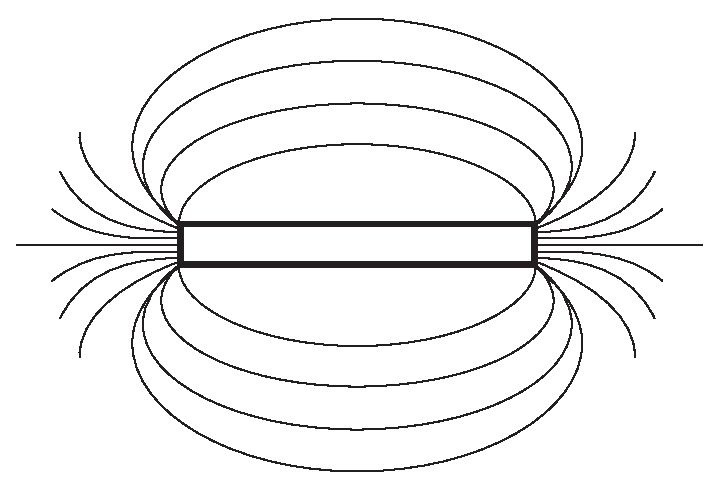
\includegraphics[width=5cm]{../magnet.eps}}
\rput(0,0){\psCoil[coilwidth=1cm,coilheight=0.5]{-1800}{1800}}
\psline(-1.75,0.5)(-2.5,0.5)(-2.5,-4)
\Ucc[labeloffset=0](-2.5,-4)(2.5,-4){A}
\psline(2.5,-4)(2.5,0.5)(1.75,0.5)
\uput[u](0,0.6){\parbox[c]{3cm}{coil with $N$ turns and
cross-sectional area, $A$}} \psline{<-}(4.8,0.4)(5.2,0.4)
\uput[d](5,-2){\parbox[c]{3cm}{magnetic field, $B$ moving to the
left.}}
\rput(3.8,0){\tiny{N}} \rput(6.1,0){\tiny{S}}
\psellipticarcn{->}(-2.8,0)(0.2,0.4){180}{-90}
\uput[l](-3,0){\parbox{1.5cm}{induced current direction}}
\end{pspicture}
\end{center}

When the north pole of a magnet is pushed into a solenoid, the
flux in the solenoid increases so the induced current will have an
associated magnetic field pointing out of the solenoid (opposite
to the magnet's field).  When the north pole is pulled out, the
flux decreases, so the induced current will have an associated
magnetic field pointing into the solenoid (same direction as the
magnet's field) to try to oppose the change. The directions of
currents and associated magnetic fields can all be found using
only the Right Hand Rule. When the fingers of the right hand are
pointed in the direction of the magnetic field, the thumb points in the
direction of the current. When the thumb is pointed in the
direction of the magnetic field, the fingers point in the
direction of the current.

\Tip{An easy way to create a magnetic field of changing
intensity is to move a permanent magnet next to a wire or coil of
wire.  The magnetic field must increase or decrease in intensity
\textit{perpendicular} to the wire (so that the magnetic field lines "cut
across" the conductor), or else no voltage will be induced.}

\Tip{Finding the direction of the induced current}{The induced
current generates a magnetic field. The induced magnetic field is
in a direction that tends to cancel out the change in the magnetic field in the loop of wire. So, you can use the Right Hand Rule to find
the direction of the induced current by remembering that the
induced magnetic field is opposite in direction to the change in the magnetic
field.}

Electromagnetic induction is put into practical use in the
construction of electrical generators, which use mechanical power
to move a magnetic field past coils of wire to generate voltage.
However, this is by no means the only practical use for this
principle.
 
If we recall that the magnetic field produced by a
current-carrying wire is always perpendicular to the wire, and
that the flux intensity of this magnetic field varies with the
amount of current which passes through it, we can see that a wire is capable of
inducing a voltage \textit{along its own length} if the current is changing. This effect is called
\textit{self-induction}. Self-induction is when a changing magnetic field is produced by
changes in current through a wire, inducing a voltage along the
length of that same wire.
  
If the magnetic flux is enhanced
by bending the wire into the shape of a coil, and/or wrapping that
coil around a material of high permeability, this effect of
self-induced voltage will be more intense. A device constructed to
take advantage of this effect is called an \textit{inductor}, and
will be discussed in greater detail in the next chapter.

\Extension{Lenz's Law}{The induced current will create a magnetic
field that opposes the change in the magnetic flux.}

\begin{wex}
{Faraday's Law} {Consider a flat square coil with 5 turns. The
coil is 0,50~m on each side, and has a magnetic field of 0,5~T
passing through it. The plane of the coil is perpendicular to the
magnetic field: the field points out of the page. Use Faraday's
Law to calculate the induced emf, if the magnetic field is
increases uniformly from 0,5~T to 1~T in 10~s. Determine the
direction of the induced current.

} {\westep{Identify what is required} We are required to use
Faraday's Law to calculate the induced emf.

\westep{Write Faraday's Law} \nequ{\epsilon=-N\frac{\Delta
\phi}{\Delta t}}

\westep{Solve Problem}
\begin{eqnarray*}
\epsilon&=&-N\frac{\Delta \phi}{\Delta t}\\
&=&-N\frac{\phi_f-\phi_i}{\Delta t}\\
&=&-N\frac{B_f\cdot A-B_i\cdot A}{\Delta t}\\
&=&-N\frac{A(B_f -B_i)}{\Delta t}\\
&=&-(5)\frac{(0,5)^2(1-0,5)}{10}\\
&=&-0,0625~\rm{V}
\end{eqnarray*}
The induced current is anti-clockwise as viewed from the direction of the increasing magnetic field.
}
\end{wex}

\subsection{Real-life applications}
The following devices use Faraday's Law in their operation.
\begin{itemize}
\item{induction stoves}
\item{tape players}
\item{metal detectors}
\item{transformers}
\end{itemize}

\Activity{Research Project}{Real-life applications of Faraday's Law}{
Choose one of the following devices and do some research on the internet or in a library how your device works. You will need to refer to Faraday's Law in your explanation.
 \begin{itemize}
\item{induction stoves}
\item{tape players}
\item{metal detectors}
\item{transformers}
\end{itemize}}

\Exercise{Faraday's Law}{
\begin{enumerate}
\item State Faraday's Law in words and write down a mathematical relationship.
\item Describe what happens when a bar magnet is pushed into or pulled out of a solenoid connected to an ammeter. Draw pictures to support your description.
\item Use the Right Hand Rule to determine the direction of the induced current in the solenoid below.
 \begin{center}
\begin{pspicture}(-4.8,-4.6)(7.4,2)
%\psgrid
\rput(5,0){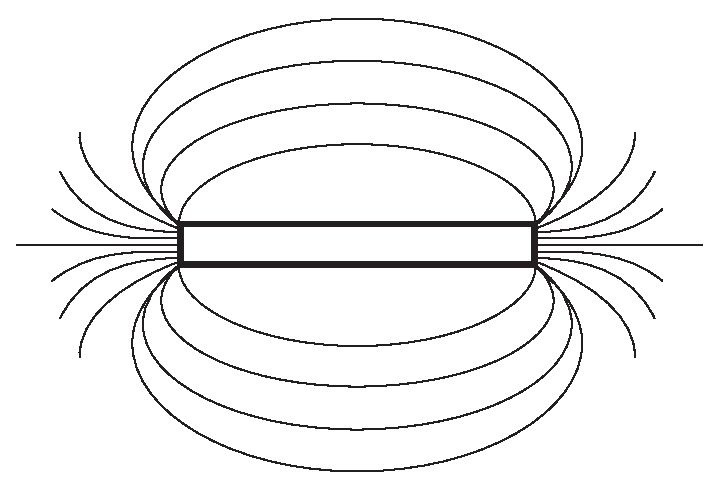
\includegraphics[width=5cm]{../magnet.eps}}
\rput(0,0){\psCoil[coilwidth=1cm,coilheight=0.5]{-1800}{1800}}
\psline(-1.75,0.5)(-2.5,0.5)(-2.5,-4)
\Ucc[labeloffset=0](-2.5,-4)(2.5,-4){A}
\psline(2.5,-4)(2.5,0.5)(1.75,0.5)
\uput[u](0,0.6){\parbox[c]{3cm}{coil with $N$ turns and
cross-sectional area, $A$}} \psline{<-}(4.8,0.4)(5.2,0.4)
\rput(3.8,0){\tiny{S}} \rput(6.1,0){\tiny{N}}
\end{pspicture}
\end{center}
\end{enumerate}
}


\section{Transformers}
%\begin{syllabus}
%\item Draw a sketch of the main features of a transformer
%\item Use Faraday's Law to explain how a transformer works in words and pictures.
%\item Use the equation for Faraday's Law to derive an expression involving the ratio between the voltages and number of windings in the primary and secondary coils.
%\item Use the expression Vs/Vp = Ns/Np to perform calculations for transformers with various specifications.
%\item State the difference between a step up and a step down transformer in both structure and function.
%\item Give an example of the use of transformers
%\item Note: The essential features of a transformer are two coils of wire, called the primary and the secondary, which are wound around different sections of the same iron core. When an alternating voltage is applied to the primary coil it creates an alternating current in that coil, which induces an alternating magnetic field in the iron core.  This changing magnetic field induces an emf, which creates a current in the secondary coil.Transformers are very important in the supply of electricity nationally. In order to reduce energy losses due to heating, electrical energy is transported from power stations along power lines at high voltage and low current.  Transformers are used to step the voltage up from the power station to the power lines, and step it down from the power lines to buildings where it is needed.
%\item Additional Suggestions: Give circuit symbol for a transformer
%\item Additional Suggestions: Give a description of transformers in the real-world, link to the power-grid, appliances, etc that use transformers.
%\item Additional Suggestions: Lots of info for interesting facts etc. on wikipedia
%\item Additional Suggestions: At least 2 worked examples using transfromer equations
%\item Additional Suggestions: activity could be: \url{http://en.wikibooks.org/wiki/School_science/How_to_make_a_transformer}
%\end{syllabus}

One of the real-world applications of Faraday's Law is in a
\textit{transformer}.
 
Eskom generates electricity at around 22~000~V. When you plug in a
toaster, the mains voltage is 220~V. A transformer is used to
\textit{step-down} the high voltage to the lower voltage that is
used as mains voltage.

\Definition{Transformer}{A transformer is an electrical device
that uses the principle of induction between the primary coil and
the secondary coil to either step-up or step-down the voltage.}

The essential features of a transformer are two coils of wire,
called the primary coil and the secondary coil, which are wound around
different sections of the same iron core.

\begin{center}
\begin{pspicture}(-5,-2)(5,2)
%\psgrid[gridcolor=gray]
\psframe[fillcolor=lightgray,fillstyle=solid](-2,-2)(2,2)
\psframe[fillcolor=white,fillstyle=solid](-1,-1)(1,1)
\psframe[linestyle=dashed,linearc=0.5cm](-1.5,-1.5)(1.5,1.5)
\psline(-4,1)(-2,1)
\multirput(0,0)(0,0.2){9}{\psline(-2,-1)(-1,-0.6)}
\psline(-4,-1)(-2,-1)

\psline(4,1)(2,1) \multirput(0,0)(0,0.2){9}{\psline(1,-0.6)(2,-1)}
\psline(4,-1)(2,-1)

\rput(0,1.9){iron core} \uput[u](-3.2,0){primary coil}
\uput[u](3.2,0){secondary coil} \uput{0.1cm}[u](0,-1.5){magnetic
flux}
%\uput[u](0,2){Main features of a transformer}
\end{pspicture}
\end{center}

When an alternating voltage is applied to the primary coil it
creates an alternating current in that coil, which induces an
alternating magnetic field in the iron core.  The changing
magnetic flux through the secondary coil induces an emf, which creates a current in this secondary coil.

The circuit symbol for a transformer is:

\begin{center}
\begin{pspicture}(2.5,2.5)
%\psgrid
\psset{unit=0.5} \pnode(0,5){A} \pnode(0,0){B} \pnode(5,5){C}
\pnode(5,0){D} \transformer(A)(B)(C)(D){$\mathcal T$}
\end{pspicture}
\end{center}

By choosing the number of coils in the secondary solenoid relative to the number of coils in the primary solenoid, we can choose how much bigger or smaller the induced secondary current is by comparison to the current in the primary solenoid (so by how much the current is stepped up or down.)

This ability to transform
voltage and current levels according to a simple ratio, determined
by the ratio of input and output coil turns is a very useful property of transformers and accounts for the name. We can derive a
mathematical relationship by using Faraday's law.
 
Assume that an alternating voltage ${V_p}$ is applied to the
primary coil (which has $N_p$ turns) of a transformer. The current
that results from this voltage generates a changing magnetic flux $\phi_p$.
We can then describe the emf in the primary coil by: \nequ{V_p =
N_p\frac{\Delta \phi_p}{\Delta t}} Similarly, for the secondary
coil, \nequ{V_s = N_s\frac{\Delta \phi_s}{\Delta t}}
 
If we assume that the primary and secondary windings are perfectly
coupled, then: \nequ{\phi_p = \phi_s} which means that:
\begin {equation*}
\frac{V_p}{V_s}=\frac{N_p}{N_s}
\end {equation*}

\begin{wex}{Transformer specifications}{Calculate the voltage on the secondary coil if the voltage on the primary coil is 120~V and the ratio of primary windings to secondary windings is 10:1.}{

\westep{Determine how to approach the problem} Use
\begin {equation*}
\frac{V_p}{V_s}=\frac{N_p}{N_s} 
\end {equation*}
with
\begin{itemize}
\item $V_p=120$
\item $\frac{N_p}{N_s}=\frac{10}{1}$
\end{itemize}

\westep{Rearrange equation to solve for $V_s$}
\begin{eqnarray*}
\frac{V_p}{V_s}&=&\frac{N_p}{N_s}\\
\frac{1}{V_s}&=&\frac{N_p}{N_s}\frac{1}{V_p}\\
\therefore V_s&=&\frac{1}{\frac{N_p}{N_s}}V_p
\end{eqnarray*}

\westep{Substitute values and solve for $V_s$}
\begin{eqnarray*}
V_s&=&\frac{1}{\frac{N_p}{N_s}}V_p\\
&=&\frac{1}{\frac{10}{1}}120\\
&=&12\;\rm{V}
\end{eqnarray*}

}
\end{wex}


A transformer designed to output more voltage than it takes in
across the input coil is called a \textit{step-up} transformer. A
step-up transformer has more windings on the secondary coil than
on the primary coil. This means that: \nequ{N_s>N_p}
 
Similarly, a transformer designed to output less than it takes in
across the input coil is called a \textit{step-down} transformer.
A step-down transformer has more windings on the primary coil than
on the primary coil. This means that: \nequ{N_p>N_s}
 
We use a step-up transformer to increase the voltage from the primary coil to the secondary coil. It is used at power stations to increase the voltage for the transmission lines.
A step-down transformer decreases the voltage from the primary coil to the secondary coil. It is particularly used to decrease the voltage from the transmission lines to a voltage which can be used in factories and in homes.
 
Transformer technology has made long-range electric power
distribution practical. Without the ability to efficiently step
voltage up and down, it would be cost-prohibitive to construct
power systems for anything but close-range (within a few kilometres) use.
 
As useful as transformers are, they only work with AC,
not DC. This is because the phenomenon of mutual inductance relies on
\textit{changing} magnetic fields, and direct current (DC) can
only produce steady magnetic fields, transformers simply will not
work with direct current.
 
Of course, direct current may be
interrupted (pulsed) through the primary winding of a transformer
to create a changing magnetic field (as is done in automotive
ignition systems to produce high-voltage spark plug power from a
low-voltage DC battery), but pulsed DC is not that different from
AC. Perhaps more than any other reason, this is why AC finds such
widespread application in power systems.

\subsection{Real-world applications}
Transformers are very important in the supply of electricity
nationally. In order to reduce energy losses due to heating,
electrical energy is transported from power stations along power
lines at high voltage and low current.  Transformers are used to
step the voltage up from the power station to the power lines, and
step it down from the power lines to buildings where it is needed.



\Exercise{Transformers}{
\begin{enumerate}
\item Draw a sketch of the main features of a transformer
\item Use Faraday's Law to explain how a transformer works in words and pictures.
\item Use the equation for Faraday's Law to derive an expression involving the ratios of the voltages and the number of windings in the primary and secondary coils.
\item If we have $N_p$ = 100 and $N_s$ = 50, and we connect the primary winding to a 230~V, 50Hz supply, then calculate the voltage on the secondary winding.
\item State the difference between a step-up and a step-down transformer in both structure and function.
\item Give an example of the use of transformers.
\end{enumerate}
}

\section{Motion of a charged particle in a magnetic field}
%\begin{syllabus}
%\item State that when a charged particle moves through a magnetic field it experiences a force.
%\item Use the equation F=qvB to calculate the force exerted on a charge that moves at right angles to a magnetic field.
%\item Use the Right Hand Rule to determine the direction of the force.
%\item Explain how this effect is used in a television
%\item Note: To use the Right Hand Rule to find the direction of the force the magnetic field exerts on the moving charge, point your fingers in the direction of the velocity of the charge and turn them (as if turning a screwdriver) towards the direction of the magnetic field.  Your thumb will point in the direction of the force.  If the charge is negative, the direction of the force will be opposite to the direction of your thumb.By only using the Right Hand Rule in the NCS learners are less likely to get confused than when there are different rules to remember.
%\end{syllabus}

When a charged particle moves through a magnetic field it
experiences a force. For a particle that is moving at right angles
to the magnetic field, the force is given by:
 \begin {equation*}
F = qvB
\end {equation*}
 where $q$ is the charge on the particle, $v$
is the velocity of the particle and $B$ is the magnetic field
through which the particle is moving. Thsi force is called the Lorentz force.

\begin{center}
\begin{pspicture}(0,0)(8,4)
%\psgrid
%field
\multirput(0.5,0.5)(1.5,0){5}{$\odot$}
\multirput(0.5,1.5)(1.5,0){5}{$\odot$}
\multirput(0.5,2.5)(1.5,0){5}{$\odot$}
\multirput(0.5,3.5)(1.5,0){5}{$\odot$}

\rput(2.3,2.25){$q$}
\psdot[dotscale=2](2,2.25)
\psline{->}(2,2.25)(2,1.5)
\rput(2.2,1.9){$v$}
\psline[linecolor=gray,linestyle=dashed]{->}(2,2.25)(0,2.25)
\rput(1,2){$F$}

\rput(5.8,2.25){$q$}
\psdot[dotscale=2](6,2.25)
\psline{->}(6,2.25)(6,3.5)
\rput(6.2,3){$v$}
\psline[linecolor=gray,linestyle=dashed]{->}(6,2.25)(8,2.25)
\rput(7,2){$F$}


\end{pspicture}
\end{center}

\begin{wex}{Charged particle moving in a magnetic field}{An electron travels at $150 {\rm m.s^{-1}}$ at right angles to a magnetic field of 80~000~T. What force is exerted on the electron? }{
\westep {Determine what is required}
We are required to determine the force on a moving charge in a magnetic field
\westep {Determine how to approach the problem}
We can use the formula:
\begin{equation*}
F = qvB
\end{equation*}
\westep {Determine what is given}
We are given
\begin{itemize}
\item $q = 1,6 \times 10^{-19} {\rm C}$ (The charge on an electron)
\item $v = 150 {\rm m.s^{-1}}$
\item $B = 80~000 {\rm T}$
\end{itemize}
\westep{Determine the force}
\begin{eqnarray*}
F &=& qvB\\
&=& (1,6 \times 10^{-19} {\rm C})(150 {\rm m.s^{-1}})( 80~000 {\rm T})\\
&=& 1,92 \times 10^{-12} {\rm N}
\end{eqnarray*}}
\end{wex}

\Tip{The direction of the force exerted on a charged particle moving
through a magnetic field is determined by using the Right Hand
Rule.\\
Point your first finger (index finger) in the direction of the velocity of the charge, your second finger (middle finger) in the direction of the magnetic field and then your thumb will point in the direction of
the force exerted on the charge.  If the charge is negative, the direction of the force
will be opposite to the direction of your thumb.}

\subsection{Real-world applications}
The following devices use the movement of charge in a magnetic field 
\begin{itemize}
\item old televisions (cathode ray tubes)
\item oscilloscope 
\end{itemize}

\Activity{Research Project}{Real-life applications of charges moving in a magnetic field}{
Choose one of the following devices and do some research on the internet or in a library how your device works. 
 \begin{itemize}
\item{oscilloscope}
\item{television}
\end{itemize}}

\Exercise{Lorentz Force}{
\begin{enumerate}
\item What happens to a charged particle when it moves through a magnetic field?
\item Explain how you would use the Right Hand Rule to determine the direction of the force experienced by a charged particle as it moves in a magnetic field.
\end{enumerate}
}

\section {Summary}
\begin {enumerate}
\item Electromagnetism is the study of the properties and relationship between electric currents and magnetism.
\item A current-carrying conductor will produce a magnetic field around the conductor.
\item The direction of the magnetic field is found by using the Right Hand Rule.
\item Electromagnets are temporary magnets formed by current-carrying conductors.
\item Electromagnetic induction occurs when a changing magnetic field induces a voltage in a current-carrying conductor.
\item Transformers use electromagnetic induction to alter the voltage.
\item A moving charged particle will experience a force in a magnetic field.
\end {enumerate}

\section{End of chapter exercises}
\begin {enumerate}
\item State the Right Hand Rule to determine the direction of a magnetic field around a current carrying wire and the Right Hand Rule to determine the direction of the force experienced by a moving charged particle in a magnetic field.
\item What did Hans Oersted discover about the relationship between electricity and magnetism?
\item List two uses of electromagnetism.
\item Draw a labelled diagram of an electromagnet and show the poles of the electromagnet on your sketch.
\item Transformers are useful electrical devices.
\begin{enumerate}
\item What is a transformer?
\item Draw a sketch of a step-down transformer.
\item What is the difference between a step-down and step-up transformer?
\item When would you use a step-up transformer?

\end{enumerate} 

\item Calculate the voltage on the secondary coil of a transformer if the voltage on the primary coil is 22~000~V and the ratio of primary windings to secondary windings is 500:1.

\item You find a transformer with 1000 windings on the primary coil and 200 windinds on the secondary coil.
\begin{enumerate}
\item What type of transformer is it?
\item What will be the voltage on the secondary coil if the voltage on the primary coil is 400~V?

\end{enumerate}
%\item[IEB 2005/11 HG] An electric cable consists of two long straight parallel wires separated by plastic insulating material. Each wire carries a current $I$ in the same direction (as shown in the diagram below).

%\begin{center}
%\begin{pspicture}(0,0)(6,1)
%\SpecialCoor
%\psgrid[gridcolor=lightgray]
%\def\rod{\psellipse[fillcolor=white,fillstyle=solid](0,0.2)(0.1,0.2)
%\psframe[fillcolor=white,fillstyle=solid,linestyle=none](0,0)(2,0.4)
%\psline(0,0)(2,0) \psline(0,0.4)(2,0.4)
%\rput(2,0){\psellipse[fillcolor=white,fillstyle=solid](0,0.2)(0.1,0.2)}}
%\psline[linewidth=1.5pt](0,0.2)(2,0.2) \rput(2,0){\rod}
%\rput(3,0.2){I}\psline{->}(3.2,0.2)(3.8,0.2)
%\psline[linewidth=1.5pt](4,0.2)(6,0.2) \uput[u](1,0.1){Wire B}
%\psline[linewidth=1.5pt](0,0.6)(2,0.6) \rput(2,0.4){\rod}
%\rput(3,0.6){I}\psline{->}(3.2,0.6)(3.8,0.6)
%\psline[linewidth=1.5pt](4,0.6)(6,0.6) \uput[u](1,0.5){Wire A}
%\end{pspicture}
%\end{center}
%Which of the following is \textbf{true} concerning the force of
%Wire A on Wire B?
%\begin{center}
%\begin{tabular}{|c|l|l|}\hline\hline
%&\textbf{Direction of Force}&\textbf{Origin of
%Force}\\\hline\hline (a)&towards A (attraction)&electrostatic
%force between opposite charges\\\hline (b)&towards B
%(repulsion)&electrostatic force between opposite charges\\\hline
%(c)&towards A (attraction)&magnetic force on current-carrying
%conductor\\\hline (d)&towards B (repulsion)&magnetic force on
%current-carrying conductor\\\hline
%\end{tabular}
%\end{center}

%\item[IEB 2005/11 HG1]\textbf{Force of parallel current-carrying conductors}\\
%Two long straight parallel current-carrying conductors placed 1 m
%apart from each other in a vacuum each carry a current of 1 A in
%the same direction.
%\begin{enumerate}
%\item{What is the magnitude of the force of 1 m of one conductor on the other?}
%\item{How does the force compare with that in the previous question when the %current in one of the conductors is halved, and their distance of separation is %halved?}
%\end{enumerate}

\item[IEB 2005/11 HG] An electron moving horizontally in a TV tube enters a region where there is a uniform magnetic field. This causes the electron to move along the path (shown by the solid line) because the magnetic field exerts a constant force on it. What is the direction of this magnetic field?
\begin{center}
\begin{pspicture}(-5,0)(2,6)
\SpecialCoor
%\psgrid[gridcolor=lightgray]
\psplot[plotstyle=curve,arrows=->]{-5}{2}{2 x exp 1.5 add}
\psline(2,0)(2,6) \psline[linestyle=dashed](-5,1.5)(2,1.5)
\uput[l](2,6){TV screen}
\end{pspicture}
\end{center}

\begin{enumerate}
\item{upwards (towards the top of the page)}
\item{downwards (towards the bottom of the page)}
\item{into the page}
\item{out of the page}
\end{enumerate}

\end{enumerate}


% CHILD SECTION END 



% CHILD SECTION START 

\chapter{Electric Circuits - Grade 11}
\label{p:em:ec11}


\section{Introduction}

The study of electrical circuits is essential to understand the technology that uses electricity in the real-world. This includes electricity being used for the operation of electronic devices like computers.




\section{Ohm's Law}
%\begin{syllabus}
%\item Determine the relationship between current, voltage and resistance at constant temperature using a simple circuit
%\item State the difference between Ohmic and non-Ohmic conductors, and give an example of each
%\item Solve problems using the mathematical expression of Ohm's Law, R=V/I
%\item Note: Link to Grade 10. A light bulb is a common example of a non-Ohmic conductor. Nichrome wire is an Ohmic conductor. Try to let learners do experiments in which they measure the current through, and voltage across an Ohmic and a non-Ohmic conductor. If they use nichrome wire, ensure that they only close the circuit for a very short time or else the nichrome will heat up and its resistance will change.
%\end{syllabus}

\subsection{Definition of Ohm's Law}

\Activity{Experiment}{Ohm's Law}{
\Aim{In this experiment we will look at the relationship between the current going through a resistor and the potential difference (voltage) across the same resistor.}\\
\begin{center}
\scalebox{1} % Change this value to rescale the drawing.
{
\begin{pspicture}(0,-1.96)(5.4,1.96)
\psline[linewidth=0.04cm](2.0,1.94)(2.0,0.54)
\psline[linewidth=0.12cm](2.2,1.54)(2.2,0.94)
\psline[linewidth=0.04cm](3.4,1.94)(3.4,0.54)
\psline[linewidth=0.12cm](3.6,1.54)(3.6,0.94)
\psline[linewidth=0.04cm,linestyle=dashed,dash=0.16cm 0.16cm](2.4,1.24)(3.2,1.24)
\psline[linewidth=0.04cm](2.0,1.24)(0.0,1.24)
\psline[linewidth=0.04cm](0.0,1.24)(0.0,-0.76)
\psline[linewidth=0.04cm](0.0,-0.76)(1.5,-0.76)
\psframe[linewidth=0.04,dimen=outer](2.7,-0.56)(1.5,-0.96)
\pscircle[linewidth=0.04,dimen=outer](2.1,-1.56){0.4}
\psline[linewidth=0.04cm](1.2,-0.76)(1.2,-1.56)
\psline[linewidth=0.04cm](1.2,-1.56)(1.7,-1.56)
\psline[linewidth=0.04cm](3.0,-0.76)(3.0,-1.56)
\psline[linewidth=0.04cm](3.0,-1.56)(2.5,-1.56)
\psline[linewidth=0.04cm](2.7,-0.76)(5.0,-0.76)
\psline[linewidth=0.04cm](4.9,0.74)(4.9,0.74)
\rput{-270.0}(5.34,-4.66){\pscircle[linewidth=0.04,dimen=outer](5.0,0.34){0.4}}
\psline[linewidth=0.04cm](5.0,-0.76)(5.0,-0.06)
\psline[linewidth=0.04cm](3.6,1.24)(5.0,1.24)
\psline[linewidth=0.04cm](5.0,1.24)(5.0,0.74)
\usefont{T1}{ptm}{m}{n}
\rput(5.0265627,0.35){A}
\usefont{T1}{ptm}{m}{n}
\rput(2.12625,-1.55){V}
\end{pspicture} 
}
\end{center}
\Method{
\begin{enumerate}
\item Set up the circuit according to the circuit diagram, starting with just one cell.
\item Draw the following table in your lab book.
\begin{center}
\begin{tabular}{|c|c|}\hline
Voltage, $V$ (V)	&	Current, $I$ (A)\\\hline\hline
1,5 &\\\hline
3,0 &\\\hline
4,5 &\\\hline
6,0 &\\\hline
\end{tabular}
\end{center}
\item Get your teacher to check the circuit before turning the power on.
\item Measure the current.
\item Add one more 1,5~V cell to the circuit and measure the current again.
\item Repeat until you have four cells and you have completed your table.
\item Draw a graph of voltage versus current.
\end{enumerate}
}
\Results{
\begin{enumerate}
\item Does your experimental results verify Ohm's Law? Explain.
\item How would you go about finding the resistance of an unknown resistor using only a power supply, a voltmeter and a known resistor $R_0$?
\end{enumerate}}
}

\Activity{Activity}{Ohm's Law}{If you do not have access to the equipment necessary for the Ohm's Law experiment, you can do this activity. 
\begin{center}
\begin{tabular}{|c|c|}\hline
Voltage, $V$ (V)	&	Current, $I$ (A)\\\hline\hline
3,0 & 0,4\\\hline
6,0 & 0,8\\\hline
9,0 & 1,2\\\hline
12,0 & 1,6\\\hline
\end{tabular}
\end{center}

\begin{enumerate}
\item Plot a graph of voltage (on the $x$-axis) and current (on the $y$-axis).
\end{enumerate}

\Conclusions{
\begin{enumerate}
\item What type of graph do you obtain (straight line, parabola, other curve)
\item Calculate the gradient of the graph.
\item Do your experimental results verify Ohm's Law? Explain.
\item How would you go about finding the resistance of an unknown resistor using only a power supply, a voltmeter and a known resistor $R_0$?
\end{enumerate}
}
}

An important relationship between the current, voltage and resistance in a circuit was discovered by Georg Simon Ohm and is called \textbf{Ohm's Law}.

\Definition{Ohm's Law}{The amount of electric current through a metal conductor, at a constant temperature, in a circuit is proportional to the voltage across the conductor. Mathematically, Ohm's Law is written:
\begin{equation*}
V=R\cdot I.
\end{equation*}}

Ohm's Law tells us that if a conductor is at a constant temperature, the current flowing through the conductor is proportional to the voltage across it. This means that if we plot voltage on the $x$-axis of a graph and current on the $y$-axis of the graph, we will get a straight-line. The gradient of the straight-line graph is related to the resistance of the conductor.

\begin{center}
\begin{pspicture}(-1,-1)(5,5)
%\psgrid[gridcolor=gray]
\psaxes{<->}(0,0)(5,5)
\psline{->}(0,0)(5,5)
\psline[linestyle=dashed](1.5,1.5)(3.5,1.5)(3.5,3.5)
\uput[r](3.5,2.5){$\Delta V$}
\uput[d](2.5,1.5){$\Delta I$}
\pcline[offset=0.4cm,linestyle=none](0,0)(0,5)
\aput{:U}{Voltage, $V$ (V)}
\pcline[offset=-0.4cm,linestyle=none](0,0)(5,0)
\bput{:U}{Current, $I$ (A)}
\rput(1,4){$R=\frac{\Delta V}{\Delta I}$}
\end{pspicture}
\end{center}

\subsection{Ohmic and non-ohmic conductors}

As you have seen, there is a mention of \textit{constant temperature} when we talk about Ohm's Law. This is because the resistance of some conductors changes as their temperature changes. These types of conductors are called \textit{non-ohmic} conductors, because they do not obey Ohm's Law. As can be expected, the conductors that obey Ohm's Law are called \textit{ohmic} conductors. A light bulb is a common example of a non-ohmic conductor. Nichrome wire is an ohmic conductor.

In a light bulb, the resistance of the filament wire will increase dramatically as it warms from room temperature to operating temperature. If we increase the supply voltage in a real lamp circuit, the resulting increase in current causes the filament to increase in temperature, which increases its resistance. This effectively limits the increase in current. In this case, voltage and current do not obey Ohm's Law.

The phenomenon of resistance changing with variations in temperature is one shared by almost all metals, of which most wires are made. For most applications, these changes in resistance are small enough to be ignored. In the application of metal lamp filaments, which increase a lot in temperature (up to about 1000$^\circ$C, and starting from room temperature) the change is quite large.

In general non-ohmic conductors have plots of voltage against current that are curved, indicating that the resistance is not constant over all values of voltage and current.

\begin{center}
\begin{pspicture}(-1,-1)(5,5)
%\psgrid[gridcolor=gray]
\psaxes{<->}(0,0)(5,5)
\psplot{0}{2.1}{x 2 exp}
\pcline[offset=-0.4cm,linestyle=none](0,0)(5,0)
\bput{:U}{Current, $I$ (A)}
\pcline[offset=0.4cm,linestyle=none](0,0)(0,5)
\aput{:U}{Voltage, $V$ (V)}
\uput[r](2,2){$V$ vs. $I$ for a non-ohmic conductor}
\end{pspicture}
\end{center}

\Activity{Experiment}{Ohmic and non-ohmic conductors}{Repeat the experiment as decribed in the previous section. In this case use a light bulb as a resistor. Compare your results to the ohmic resistor.}

\subsection{Using Ohm's Law}

We are now ready to see how Ohm's Law is used to analyse circuits.

Consider the circuit with an ohmic resistor, $R$. If the resistor has a resistance of 5~\ohm\ and voltage across the resistor is 5 V, then we can use Ohm's law to calculate the current flowing through the resistor. 

\begin{center}
\begin{pspicture}(0,0)(5,5)
%\psgrid[gridcolor=gray]
\pnode(1,1){A}
\pnode(4,1){B}
\pnode(4,4){C}
\pnode(1,4){D}
\battery(A)(B){}
\psline(B)(C)
\resistor[dipolestyle=rectangle](C)(D){$R$}
\psline(D)(A)
\end{pspicture}
\end{center}

Ohm's law is:
\nequ{V=R \cdot I}
which can be rearranged to:
\nequ{I=\frac{V}{R}}

The current flowing through the resistor is:
\begin{eqnarray*}
I&=&\frac{V}{R}\\
&=&\frac{5\;\mathrm{V}}{5\;\eohm}\\
&=&1\;\mathrm{A}
\end{eqnarray*}

\begin{wex}{Ohm's Law}{
\begin{center}
\begin{pspicture}(0,0)(5,5)
%\psgrid[gridcolor=gray]
\pnode(1,1){A}
\pnode(4,1){B}
\pnode(4,4){C}
\pnode(1,4){D}
\battery(A)(B){}
\psline(B)(C)
\resistor[dipolestyle=rectangle](C)(D){$R$}
\psline(D)(A)
\end{pspicture}
\end{center}
The resistance of the above resistor is 10~\ohm\ and the current going through the resistor is 4~A. What is the potential difference (voltage) across the resistor?}{

\westep{Determine how to approach the problem}
It is an Ohm's Law problem. So we use the equation:
\nequ{V=R \cdot I}

\westep{Solve the problem}
\begin{eqnarray*}
V&=&R \cdot I \\
&=&(10)(4)  \\
&=&40~V
\end{eqnarray*}
\westep{Write the final answer}
The voltage across the resistor is 40~V.}
\end{wex}

\Exercise{Ohm's Law}{
\begin{enumerate}
\item Calculate the resistance of a resistor that has a potential difference of 8~V across it when a current of 2~A flows through it.
\item What current will flow through a resistor of 6~\ohm\ when there is a potential difference of 18~V across its ends?
\item What is the voltage across a 10~\ohm\ resistor when a current of 1,5~A flows though it? 
\end{enumerate}}

\section{Resistance}
%\begin{syllabus}
%\item Calculate the equivalent resistance of series and parallel arrangements of resistors.
%\item Solve problems involving current, voltage and resistance for circuits containing arrangements of resistors in series and in parallel.
%\item State that a real battery has internal resistance
%\item Explain why there is a difference between the emf and terminal voltage of a battery if the load (external resistance in the circuit) is comparable in size to the battery's internal resistance
%\item Solve circuit problems in which the internal resistance of the battery must be considered.
%\item Note: Some books use the term "lost volts" to refer to the difference between the emf and the terminal voltage. This is misleading. The voltage is not "lost", it is across the internal resistance of the battery. The internal resistance of the battery can be treated just like another resistor in series in the circuit. The sum of the voltages across the external circuit plus the voltage across the internal resistance is equal to the emf:e = V(load) + V(internal resistance)
%\end{syllabus}

In Grade 10, you learnt about resistors and were introduced to circuits where resistors were connected in series and circuits where resistors were connected in parallel. In a series circuit there is one path for the current to flow through. In a parallel circuit there are multiple paths for the current to flow through.

\begin{center}
\begin{pspicture}(0,-1)(10,4)
%\psgrid[gridcolor=gray]
\rput(0,0){
\battery(0,0)(0,4){}
\psline(0,4)(4,4)
\resistor[dipolestyle=rectangle](4,4)(4,0){}
\resistor[dipolestyle=rectangle](4,0)(0,0){}
\uput[d](2,-0.2){series circuit}
\uput[d](2,-0.6){\small{one current path}}
%\rput(2,2){one current path}
\psarcn{<-}(2,2){1.25}{210}{-30}}

\rput(6,0){
\battery(0,0)(0,4){}
\psline(0,4)(4,4)
\resistor[dipolestyle=rectangle](4,4)(4,0){}
\resistor[dipolestyle=rectangle](2,4)(2,0){}
\psline(4,0)(0,0)
\uput[d](2,-0.2){parallel circuit}
\uput[d](2,-0.6){\small{multiple current paths}}
\psarcn{<-}(1,2){0.4}{210}{-30}
\psarcn{<-}(3,2){0.4}{210}{-30}
}

\end{pspicture}
\end{center}

\subsection{Equivalent resistance}
When there is more than one resistor in a circuit, we are usually able to calculate the total combined resitance of all the resistors. The resistance of the single resistor is known as \textit{equivalent resistance}.

\subsubsection{Equivalent Series Resistance}
Consider a circuit consisting of three resistors and a
single cell connected in series. 

\begin{center}
\begin{pspicture}(0,0)(5,5)
%\psgrid
\pnode(1,4){A}
\pnode(4,4){B}
\pnode(4,1){C}
\pnode(1,1){D}
\resistor[dipolestyle=rectangle](A)(B){R$_{1}$}
\resistor[labeloffset=1.2cm,dipolestyle=rectangle](B)(C){R$_{2}$}
\resistor[dipolestyle=rectangle](C)(D){R$_{3}$}
\battery[labeloffset=1cm](A)(D){$V$}
\uput[ul](A){A}
\uput[ur](B){B}
\uput[dr](C){C}
\uput[dl](D){D}
\psdots(A)(B)(C)(D)
\end{pspicture}
\end{center}

The first principle to understand about series circuits is that the amount of current is the same through any component in the circuit. This is because there is only one path for electrons to flow in a series circuit. From the way that the battery is connected, we can tell which direction the current will flow. We know that current flows from positive to negative, by convention. Current in this circuit will flow in a clockwise direction, from point A to B to C to D and back to A.

So, how do we use this knowledge to calculate the total resistance in the circuit?

We know that in a series circuit the current has to be the same in all components. So we can write:

\begin{equation*}
\label{eq:seriesR:I}
I = I_1 =I_2=I_3
\end{equation*}

We also know that total voltage of the circuit has to be equal to the sum of the voltages over all three resistors. So we can write:

\begin{equation*}
\label{eq:seriesR:V}
V=V_1+V_2+V_3
\end{equation*}

Finally, we know that Ohm's Law has to apply for each resistor individually, which gives us:

\begin{eqnarray*}
V_1 & = & I_1\cdot R_1 \\
V_2 & = & I_2\cdot R_2 \\
V_3 & = & I_3\cdot R_3
\end{eqnarray*}
Therefore:

\begin{equation*}
V=I_1\cdot R_1+I_2\cdot R_2+I_3\cdot R_3
\end{equation*}
However, because
\begin{equation*}
I = I_1 =I_2=I_3
\end{equation*} , we can further simplify this to:

\begin{eqnarray*}
V&=&I \cdot R_1+ I \cdot R_2+I  \cdot R_3\\
&=&I (R_1+R_2+R_3)
\end{eqnarray*}
Further, we can write an Ohm's Law relation for the entire circuit:
\nequ{V=I\cdot R}
Therefore:
\begin{eqnarray*}
V&=&I (R_1+R_2+R_3)\\
I\cdot R&=&I (R_1+R_2+R_3)\\
\therefore\quad R&=&R_1+R_2+R_3
\end{eqnarray*}

\Definition{Equivalent resistance in a series circuit, $R_s$}
{For $n$ resistors in series the equivalent resistance is:
\begin{equation*}
\label{eq:seriesR:R}
R_s=R_{1}+R_{2}+R_{3}+\cdots+R_n
\end{equation*}}
Let us apply this to the following circuit.

\begin{center}
\begin{pspicture}(0,0)(5,5)
%\psgrid
\pnode(1,4){A}
\pnode(4,4){B}
\pnode(4,1){C}
\pnode(1,1){D}
\resistor[dipolestyle=rectangle](A)(B){R$_{1}$=3~\ohm}
\resistor[labeloffset=1.2cm,dipolestyle=rectangle](B)(C){R$_{2}$=10~\ohm}
\resistor[dipolestyle=rectangle](C)(D){R$_{3}$=5~\ohm}
\battery[labeloffset=1cm](A)(D){9~V}
\uput[ul](A){A}
\uput[ur](B){B}
\uput[dr](C){C}
\uput[dl](D){D}
\psdots(A)(B)(C)(D)
\end{pspicture}
\end{center}

The resistors are in series, therefore:
\begin{eqnarray*}
R_s&=&R_{1}+R_{2}+R_{3}\\
&=&3\eohm+10\eohm+5\eohm\\
&=&18\eohm
\end{eqnarray*}

\begin{wex}{Equivalent series resistance I}{Two 10~k\ohm\ resistors are connected in series. Calculate the equivalent resistance.}{

\westep{Determine how to approach the problem}
Since the resistors are in series we can use:
\nequ{R_s=R_{1}+R_{2}}

\westep{Solve the problem}
\begin{eqnarray*}
R_s&=&R_{1}+R_{2}\\
&=&10\,\rm{k}\eohm+10\,\rm{k}\eohm\\
&=&20\,\rm{k}\eohm
\end{eqnarray*}

\westep{Write the final answer}
The equivalent resistance of two 10~k\ohm\ resistors connected in series is 20~k\ohm.}
\end{wex}

\begin{wex}{Equivalent series resistance II}{Two resistors are connected in series. The equivalent resistance is 100~\ohm. If one resistor is 10~\ohm, calculate the value of the second resistor.}{

\westep{Determine how to approach the problem}
Since the resistors are in series we can use:
\nequ{R_s=R_{1}+R_{2}}
We are given the value of $R_s$ and $R_1$.

\westep{Solve the problem}
\begin{eqnarray*}
R_s&=&R_{1}+R_{2}\\
\therefore\quad R_2&=&R_s-R_1\\
&=&100\eohm-10\eohm\\
&=&90\eohm
\end{eqnarray*}

\westep{Write the final answer}
The second resistor has a resistance of 90~\ohm.}
\end{wex}

\subsubsection{Equivalent parallel resistance}
Consider a circuit consisting of a single cell and three resistors that are connected in parallel. 

\begin{center}
\begin{pspicture}(0,1)(8,4)
%\psgrid
\pnode(1,4){A}
\pnode(3,4){B}
\pnode(5,4){C}
\pnode(7,4){D}
\pnode(7,1){E}
\pnode(5,1){F}
\pnode(3,1){G}
\pnode(1,1){H}
\resistor[dipolestyle=rectangle](B)(G){R$_{1}$}
\resistor[dipolestyle=rectangle](C)(F){R$_{2}$}
\resistor[dipolestyle=rectangle](D)(E){R$_{3}$}
\battery(A)(H){$V$}
\psline(A)(D)
\psline(H)(E)
\uput[u](1,4){A}
\uput[u](3,4){B}
\uput[u](5,4){C}
\uput[u](7,4){D}
\uput[d](7,1){E}
\uput[d](5,1){F}
\uput[d](3,1){G}
\uput[d](1,1){H}
\psdots(A)(B)(C)(D)(E)(F)(G)(H)
\end{pspicture}
\end{center}

The first principle to understand about parallel circuits is that the
voltage is equal across all components in the circuit. This is because there are only two sets of electrically common points in a parallel circuit, and voltage measured between sets of common points must always be the same at any given time. So, for the circuit shown, the following is true: 

\begin{equation*}
\label{eq:parallelR:V}
V=V_1=V_2=V_3
\end{equation*}

The second principle for a parallel circuit is that all the currents through each resistor must add up to the total current in the circuit. 

\begin{equation*}
\label{eq:parallelR:I}
I=I_1+I_2+I_3
\end{equation*}

Also, from applying Ohm's Law to the entire circuit, we can write:
\begin{equation*}
V=\frac{I}{R_p}
\end{equation*}
where $R_p$ is the equivalent resistance in this parallel arrangement.

We are now ready to apply Ohm's Law to each resistor, to get:
\begin{eqnarray*}
V_1&=&R_1\cdot I_1\\
V_2&=&R_2\cdot I_2\\
V_3&=&R_3\cdot I_3
\end{eqnarray*}
This can be also written as:
\begin{eqnarray*}
I_1&=&\frac{V_1}{R_1}\\
I_2&=&\frac{V_2}{R_2}\\
I_3&=&\frac{V_3}{R_3}
\end{eqnarray*}

Now we have:
\begin{eqnarray*}
I&=&I_1+I_2+I_3\\
\frac{V}{R_p}&=&\frac{V_1}{R_1}+\frac{V_2}{R_2}+\frac{V_3}{R_3}\\
&=&\frac{V}{R_1}+\frac{V}{R_2}+\frac{V}{R_3}\\ 
\rm{because} & & V=V_1=V_2=V_3 \\
&=&V\left(\frac{1}{R_1}+\frac{1}{R_2}+\frac{1}{R_3}\right)\\
\therefore \quad \frac{1}{R_p}&=&\left(\frac{1}{R_1}+\frac{1}{R_2}+\frac{1}{R_3}\right)
\end{eqnarray*}

\Definition{Equivalent resistance in a parallel circuit, $R_p$}{For $n$ resistors in parallel, the equivalent resistance is:
\begin{equation*}
\label{eq:parallelR:R}
\frac{1}{R_p}=\left(\frac{1}{R_1}+\frac{1}{R_2}+\frac{1}{R_3}+\cdots+\frac{1}{R_n}\right)
\end{equation*}}

Let us apply this formula to the following circuit.

\begin{center}
\begin{pspicture}(0,1)(8,4)
%\psgrid
\pnode(1,4){A}
\pnode(3,4){B}
\pnode(5,4){C}
\pnode(7,4){D}
\pnode(7,1){E}
\pnode(5,1){F}
\pnode(3,1){G}
\pnode(1,1){H}
\resistor[labeloffset=1cm,dipolestyle=rectangle](B)(G){R$_{1}$=10\ohm}
\resistor[labeloffset=1cm,dipolestyle=rectangle](C)(F){R$_{2}$=2\ohm}
\resistor[labeloffset=1cm,dipolestyle=rectangle](D)(E){R$_{3}$=1\ohm}
\battery[labeloffset=1cm](A)(H){$V$=9~V}
\psline(A)(D)
\psline(H)(E)
\end{pspicture}
\end{center}

What is the total resistance in the circuit?

\begin{eqnarray*}
\frac{1}{R_p}&=&\left(\frac{1}{R_1}+\frac{1}{R_2}+\frac{1}{R_3}\right)\\
&=&\left(\frac{1}{10\eohm}+\frac{1}{2\eohm}+\frac{1}{1\eohm}\right)\\
&=&\left(\frac{1+5+10}{10}\right)\\
&=&\left(\frac{16}{10}\right)\\
\therefore\quad R_p&=&0,625\eohm
\end{eqnarray*}

\subsection{Use of Ohm's Law in series and parallel Circuits}
\begin{wex}{Ohm's Law}
{Calculate the current ($I$) in this circuit if the resistors are both ohmic in nature.}
{
\begin{center}
\begin{pspicture}(0,0)(5,5)
%\psgrid[gridcolor=gray]
\pnode(1,1){A}
\pnode(4,1){B}
\pnode(4,4){C}
\pnode(1,4){D}
\battery(A)(B){$V$=12~V}
\psline(B)(C)
\resistor[dipolestyle=rectangle](C)(D){$R_1$=2~\ohm}
\resistor[labeloffset=-0.9cm](D)(A){$R_2$=4~\ohm}
\pcline{<-}(1,0.5)(2,0.5)
\bput{:U}{I}
\end{pspicture}
\end{center}
}
{
\westep{Determine what is required}
We are required to calculate the current flowing in the circuit.

\westep{Determine how to approach the problem}
Since the resistors are Ohmic in nature, we can use Ohm's Law. There are however two resistors in the circuit and we need to find the total resistance. 

\westep{Find total resistance in circuit}
Since the resistors are connected in series, the total resistance $R$ is:
\nequ{R=R_1+R_2}

Therefore, 
\nequ{R=2+4=6\;\eohm}

\westep{Apply Ohm's Law}
\begin{eqnarray*}
V&=&R\cdot I\\
\therefore\quad I&=&\frac{V}{R}\\
&=&\frac{12}{6}\\
&=&2\;\mathrm{A}
\end{eqnarray*}

\westep{Write the final answer}
A 2~A current is flowing in the circuit.}
\end{wex}

\begin{wex}{Ohm's Law I}
{Calculate the current ($I$) in this circuit if the resistors are both ohmic in nature.}
{
\begin{center}
\begin{pspicture}(0,0)(5,5)
%\psgrid[gridcolor=gray]
\pnode(1,1){A}
\pnode(4,1){B}
\pnode(4,4){C}
\pnode(1,4){D}
\pnode(1,2.5){E}
\pnode(4,2.5){F}
\battery(A)(B){$V$=12~V}
\psline(B)(C)
\resistor[dipolestyle=rectangle](D)(C){$R_1$=2~\ohm}
\resistor[dipolestyle=rectangle](E)(F){$R_2$=4~\ohm}
\psline(D)(A)
\pcline{<-}(1,0.5)(2,0.5)
\bput{:U}{I}
\end{pspicture}
\end{center}
}
{
\westep{Determine what is required}
We are required to calculate the current flowing in the circuit.

\westep{Determine how to approach the problem}
Since the resistors are Ohmic in nature, we can use Ohm's Law. There are however two resistors in the circuit and we need to find the total resistance. 

\westep{Find total resistance in circuit}
Since the resistors are connected in parallel, the total resistance $R$ is:
\nequ{\frac{1}{R}=\frac{1}{R_1}+\frac{1}{R_2}}
Therefore, 
\begin{eqnarray*}
\frac{1}{R}&=&\frac{1}{R_1}+\frac{1}{R_2}\\
&=&\frac{1}{2}+\frac{1}{4}\\
&=&\frac{2+1}{4}\\
&=&\frac{3}{4}\\
Therefore, R&=&1,33\;\eohm
\end{eqnarray*}

\westep{Apply Ohm's Law}
\begin{eqnarray*}
V&=&R\cdot I\\
\therefore\quad I&=&\frac{V}{R}\\
&=&\frac{12}{\frac{4}{3}}\\
&=&9\;\mathrm{A}
\end{eqnarray*}

\westep{Write the final answer}
A 9~A current is flowing in the circuit.}
\end{wex}

\begin{wex}{Ohm's Law II}
{Two ohmic resistors ($R_1$ and $R_2$) are connected in series with a cell. Find the resistance of $R_2$, given that the current flowing through $R_1$ and $R_2$ is 0,25~A and that the voltage across the cell is 1,5~V. $R_1$=1~\ohm.}
{\westep{Draw the circuit and fill in all known values.}

\begin{center}
\begin{pspicture}(0,0)(5,5)
%\psgrid[gridcolor=gray]
\pnode(1,1){A}
\pnode(4,1){B}
\pnode(4,4){C}
\pnode(1,4){D}
\battery(A)(B){$V$=1,5~V}
\psline(B)(C)
\resistor[dipolestyle=rectangle](C)(D){$R_1$=1~\ohm}
\resistor[labeloffset=-0.9cm](D)(A){$R_2$=?}
\pcline{<-}(1,0.5)(2,0.5)
\bput{:U}{$I$=0,25~A}
\end{pspicture}
\end{center}

\westep{Determine how to approach the problem.}
We can use Ohm's Law to find the total resistance $R$ in the circuit, and then calculate the unknown resistance using:
\nequ{R=R_1+R_2} 
because it is in a series circuit.

\westep{Find the total resistance}
\begin{eqnarray*}
V&=&R\cdot I\\
\therefore\quad R&=&\frac{V}{I}\\
&=&\frac{1,5}{0,25}\\
&=&6\eohm
\end{eqnarray*}

\westep{Find the unknown resistance}
We know that:
\nequ{R=6\eohm}
and that 
\nequ{R_1=1\eohm}
Since 
\nequ{R=R_1+R_2}
\nequ{R_2=R-R_1} 
Therefore,
\nequ{R_2=5\eohm} 
}
\end{wex}

\subsection{Batteries and internal resistance}

Real batteries are made from materials which have resistance. This means that real batteries are not just sources of potential difference (voltage), but they also possess internal resistance. If the total voltage source is referred to as the emf, ${\cal E}$, then a real battery can be represented as an emf  connected in series with a resistor $r$. The internal resistance of the battery is represented by the symbol $r$. 

\begin{center}
\begin{pspicture}(0,0)(5,5)
%\psgrid[gridcolor=gray]
\pnode(1,1){A}
\pnode(4,1){B}
\pnode(4,4){C}
\pnode(1,4){D}
\pnode(2.5,1){E}
\battery(A)(E){$\mathcal{E}$}
\resistor[unit=0.5,dipolestyle=rectangle](E)(B){$r$}
\psline(B)(C)
\resistor[dipolestyle=rectangle](C)(D){$R$}
\psline(D)(A)
\psframe[linestyle=dashed](1.4,0.4)(3.8,2)
\uput[d](2.5,0.4){$V$}
\end{pspicture}
\end{center}

\Definition{Load}{The external resistance in the circuit is referred to as the load.}

Suppose that the battery with emf $\mathcal{E}$ and internal resistance $r$ supplies a current $I$ through an external load resistor $R$. Then the voltage drop across the load resistor is that supplied by the battery:
\nequ{V=I\cdot R}
Similarly, from Ohm's Law, the voltage drop across the internal resistance is: 
\nequ{V_r=I\cdot r}

The voltage $V$ of the battery is related to its emf ${\cal E}$ and internal resistance $r$ by:
\begin{eqnarray*}
{\cal E} &=& V + I r ;or\\
V&=& {\cal E} - I r
\end{eqnarray*}

The emf of a battery is essentially constant because it only depends on the chemical reaction (that converts chemical energy into electrical energy) going on inside the battery. Therefore, we can see that the voltage across the terminals of the battery is dependent on the current drawn by the load. The higher the current, the lower the voltage across the terminals, because the emf is constant. By the same reasoning, the voltage only equals the emf when the current is very small.

The maximum current that can be drawn from a battery is limited by a critical value $I_c$. At a current of $I_c$, $V$=0~V. Then, the equation becomes:
\begin{eqnarray*}
0 &=& {\cal E} - I_c r\\
I_c r &=& {\cal E}\\
I_c&=&\frac{{\cal E}}{r}
\end{eqnarray*}
The maximum current that can be drawn from a battery is less than $\frac{{\cal E}}{r}$.


\begin{wex}{Internal resistance}{What is the internal resistance of a battery if its emf is 12~V and the voltage drop across its terminals is 10~V when a current of 4~A flows in the circuit when it is connected across a load?}{
\westep{Determine how to approach the problem}
It is an internal resistance problem. So we use the equation:
\begin{eqnarray*}
{\cal E} &=& V + I r
\end{eqnarray*}

\westep{Solve the problem}
\begin{eqnarray*}
{\cal E} &=& V + I r\\
12&=&10 + 4(r)\\ 
&=&0.5
\end{eqnarray*}

\westep{Write the final answer}
The internal resistance of the resistor is 0.5~\ohm.}
\end{wex}

\Exercise{Resistance}{
\begin{enumerate}
\item Calculate the equivalent resistance of:
\begin{enumerate}
\item three 2~\ohm\ resistors in series;
\item two 4~\ohm\ resistors in parallel;
\item a 4~\ohm\ resistor in series with a 8~\ohm\ resistor;
\item a 6~\ohm\ resistor in series with two resistors (4~\ohm\ and 2~\ohm\ ) in parallel.
\end{enumerate}
\item Calculate the total current in this circuit if both resistors are ohmic.
\begin{center}
\begin{pspicture}(0,0)(5,5)
%\psgrid[gridcolor=gray]
\pnode(1,1){A}
\pnode(4,1){B}
\pnode(4,4){C}
\pnode(1,4){D}
\pnode(1,2.5){E}
\pnode(4,2.5){F}
\battery(A)(B){$V$=9~V}
\psline(B)(C)
\resistor[dipolestyle=rectangle](D)(C){$R_1$=3~\ohm}
\resistor[dipolestyle=rectangle](E)(F){$R_2$=6~\ohm}
\psline(D)(A)
\pcline{<-}(1,0.5)(2,0.5)
\bput{:U}{I}
\end{pspicture}
\end{center}
\item Two ohmic resistors are connected in series. The resistance of the one resistor is 4~\ohm\ . What is the resistance of the other resistor if a current of 0,5~A flows through the resistors when they are connected to a voltage supply of 6~V. 
\item Describe what is meant by the \textit{internal resistance} of a real battery.
\item Explain why there is a difference between the emf and terminal voltage of a battery if the load (external resistance in the circuit) is comparable in size to the battery's internal resistance
\item What is the internal resistance of a battery if its emf is 6~V and the voltage drop across its terminals is 5,8~V when a current of 0,5~A flows in the circuit when it is connected across a load?
\end{enumerate}}

\section{Series and parallel networks of resistors}
%\begin{syllabus}
%\item Solve circuit problems involving resistors in series with parallel networks of resistors
%\item Note: A parallel network is an arrangement of resistors that are in parallel with each other but not with the battery. A circuit containing one or more resistors in series with parallel network(s) is a series-parallel circuit
%\end{syllabus}

Now that you know how to handle simple series and parallel circuits, you are ready to tackle problems like this:

\begin{figure}[htbp]
\begin{center}
\begin{pspicture}(-0.6,-0.8)(6.6,4)
%\psgrid[gridcolor=lightgray]
\psset{unit=0.75}
\pnode(0,0){A}
\pnode(0,4){B}
\pnode(2,4){C}
\pnode(3,4.75){D}
\pnode(3,3.25){E}
\pnode(5,4.75){F}
\pnode(6,4){G}
\pnode(5,3.25){H}
\pnode(8,4){I}
\pnode(8,0){J}
\pnode(5,0.75){K}
\pnode(6,0){L}
\pnode(5,-0.75){M}
\pnode(2,0){O}
\pnode(3,0.75){P}
\pnode(3,-0.75){N}

\battery(A)(B){}
\psline(B)(C)
\psline(C)(D)\resistor[unit=0.5,dipolestyle=rectangle](D)(F){$R_1$}\psline(F)(G)
\resistor[unit=0.5,dipolestyle=rectangle](C)(G){$R_2$}
\psline(C)(E)\resistor[unit=0.5,dipolestyle=rectangle](E)(H){$R_3$}\psline(H)(G)
\psline(G)(I)
\resistor[unit=0.5,dipolestyle=rectangle](I)(J){$R_4$}
\psline(J)(L)
\psline(L)(K)\resistor[unit=0.5,dipolestyle=rectangle](K)(P){\small{$R_5$}}\psline(P)(O)
\resistor[unit=0.5,dipolestyle=rectangle](L)(O){$R_6$}
\psline(L)(M)\resistor[unit=0.5,dipolestyle=rectangle](M)(N){$R_7$}\psline(N)(O)
\psline(O)(A)
\psframe[linestyle=dashed](1.8,-1)(6.2,1)
\uput[u](4,1){Parallel Circuit 1}
\psframe[linestyle=dashed](1.8,3)(6.2,5)
\uput[d](4,3){Parallel Circuit 2}
\end{pspicture}
\end{center}
\caption{An example of a series-parallel network. The dashed boxes indicate parallel sections of the circuit.}
\label{fig:serpar}
\end{figure}

It is relatively easy to work out these kind of circuits because you use everything you have already learnt about series and parallel circuits. The only difference is that you do it in stages. In Figure~\ref{fig:serpar}, the circuit consists of 2 parallel portions that are then in series with 1 resistor. So, in order to work out the equivalent resistance, you start by calculating the total resistance of the parallel portions and then add up all the resistances in series. If all the resistors in Figure~\ref{fig:serpar} had resistances of 10~\ohm, we can calculate the equivalent resistance of the entire circuit.

We start by calculating the total resistance of \textit{Parallel Circuit 1}.

\begin{center}
\begin{pspicture}(-0.6,-0.8)(6.6,4)
%\psgrid[gridcolor=lightgray]
\psset{unit=0.75}
\pnode(0,0){A}
\pnode(0,4){B}
\pnode(2,4){C}
\pnode(3,4.75){D}
\pnode(3,3.25){E}
\pnode(5,4.75){F}
\pnode(6,4){G}
\pnode(5,3.25){H}
\pnode(8,4){I}
\pnode(8,0){J}
\pnode(5,0.75){K}
\pnode(6,0){L}
\pnode(5,-0.75){M}
\pnode(2,0){O}
\pnode(3,0.75){P}
\pnode(3,-0.75){N}

\battery(A)(B){}
\psline(B)(C)
%\psline(C)(D)\resistor[unit=0.5,dipolestyle=rectangle](D)(F){$R_1$}\psline(F)(G)
\resistor[unit=0.5,dipolestyle=rectangle](C)(G){$R_{p1}$}
%\psline(C)(E)\resistor[unit=0.5,dipolestyle=rectangle](E)(H){$R_3$}\psline(H)(G)
\psline(G)(I)
\resistor[unit=0.5,dipolestyle=rectangle](I)(J){$R_4$}
\psline(J)(L)
\psline(L)(K)\resistor[unit=0.5,dipolestyle=rectangle](K)(P){\small{$R_5$}}\psline(P)(O)
\resistor[unit=0.5,dipolestyle=rectangle](L)(O){$R_6$}
\psline(L)(M)\resistor[unit=0.5,dipolestyle=rectangle](M)(N){$R_7$}\psline(N)(O)
\psline(O)(A)
\end{pspicture}
\end{center}

The value of $R_{p1}$ is:
\begin{eqnarray*}
\frac{1}{R_{p1}}&=&\frac{1}{R_1}+\frac{1}{R_2}+\frac{1}{R_3}\\
R_{p1}&=&\left(\frac{1}{10}+\frac{1}{10}+\frac{1}{10}\right)^{-1}\\
&=&\left(\frac{1+1+1}{10}\right)^{-1}\\
&=&\left(\frac{3}{10}\right)^{-1}\\
&=&3,33\eohm
\end{eqnarray*}

We can similarly calculate the total resistance of \textit{Parallel Circuit 2}:
\begin{eqnarray*}
\frac{1}{R_{p2}}&=&\frac{1}{R_5}+\frac{1}{R_6}+\frac{1}{R_7}\\
R_{p2}&=&\left(\frac{1}{10}+\frac{1}{10}+\frac{1}{10}\right)^{-1}\\
&=&\left(\frac{1+1+1}{10}\right)^{-1}\\
&=&\left(\frac{3}{10}\right)^{-1}\\
&=&3,33\eohm
\end{eqnarray*}

\begin{center}
\begin{pspicture}(-0.6,-0.8)(6.6,4)
%\psgrid[gridcolor=lightgray]
\psset{unit=0.75}
\pnode(0,0){A}
\pnode(0,4){B}
\pnode(2,4){C}
\pnode(3,4.75){D}
\pnode(3,3.25){E}
\pnode(5,4.75){F}
\pnode(6,4){G}
\pnode(5,3.25){H}
\pnode(8,4){I}
\pnode(8,0){J}
\pnode(5,0.75){K}
\pnode(6,0){L}
\pnode(5,-0.75){M}
\pnode(2,0){O}
\pnode(3,0.75){P}
\pnode(3,-0.75){N}

\battery(A)(B){}
\psline(B)(C)
\resistor[unit=0.5,dipolestyle=rectangle](C)(G){$R_{p1}=\frac{10}{3}\eohm$}
\psline(G)(I)
\resistor[unit=0.5,dipolestyle=rectangle](I)(J){$R_4=10\eohm$}
\psline(J)(L)
\resistor[unit=0.5,dipolestyle=rectangle](L)(O){$R_{p2}=\frac{10}{3}\eohm$}
\psline(O)(A)
\end{pspicture}
\end{center}

This has now being simplified to a simple series circuit and the equivalent resistance is:
\begin{eqnarray*}
R&=&R_{p1}+R_4+R_{p2}\\
&=&\frac{10}{3}+10+\frac{10}{3}\\
&=&\frac{100+30+100}{30}\\
&=&\frac{230}{30}\\
&=&7,66\eohm
\end{eqnarray*}

The equivalent resistance of the circuit in Figure~\ref{fig:serpar} is 7,66$\eohm$.

\Exercise{Series and parallel networks}{
Determine the equivalent resistance of the following circuits:
\begin{enumerate}
\item  { 
\scalebox{1} % Change this value to rescale the drawing.
{
\begin{pspicture}(0,-2.0289063)(5.62,2.0089064)
\psline[linewidth=0.04cm](2.5,1.9889063)(2.5,0.5889062)
\psline[linewidth=0.12cm](2.7,1.5889063)(2.7,0.98890626)
\psline[linewidth=0.04cm](2.5,1.2889062)(0.0,1.2889062)
\psline[linewidth=0.04cm](0.0,1.2889062)(0.0,-0.7110937)
\psline[linewidth=0.04cm](0.0,-0.7110937)(0.8,-0.7110937)
\psframe[linewidth=0.04,dimen=outer](2.0,-0.51109374)(0.8,-0.9110938)
\psline[linewidth=0.04cm](2.0,-0.7110937)(2.7,-0.7110937)
\psline[linewidth=0.04cm](4.9,0.7889063)(4.9,0.7889063)
\psline[linewidth=0.04cm](2.7,-1.3110938)(2.7,-0.11109375)
\psline[linewidth=0.04cm](2.7,1.2889062)(5.6,1.2889062)
\psline[linewidth=0.04cm](5.6,1.2889062)(5.6,-0.7110937)
\psline[linewidth=0.04cm](2.7,-0.11109375)(3.2,-0.11109375)
\psline[linewidth=0.04cm](2.7,-1.3110938)(3.2,-1.3110938)
\psframe[linewidth=0.04,dimen=outer](4.4,0.08890625)(3.2,-0.31109375)
\psframe[linewidth=0.04,dimen=outer](4.4,-1.1110938)(3.2,-1.5110937)
\psline[linewidth=0.04cm](5.6,-0.7110937)(4.9,-0.7110937)
\psline[linewidth=0.04cm](4.9,-1.3110938)(4.9,-0.11109375)
\psline[linewidth=0.04cm](4.9,-0.11109375)(4.4,-0.11109375)
\psline[linewidth=0.04cm](4.9,-1.3110938)(4.4,-1.3110938)
\usefont{T1}{ptm}{m}{n}
\rput(1.4670312,-1.2010938){2 $\Omega$}
\usefont{T1}{ptm}{m}{n}
\rput(3.8670313,-1.8010937){2 $\Omega$}
\usefont{T1}{ptm}{m}{n}
\rput(3.868125,0.29890624){4 $\Omega$}
\end{pspicture} 
}
}
\item {
\scalebox{1} % Change this value to rescale the drawing.
{
\begin{pspicture}(0,-1.9789063)(8.439688,1.9589063)
\psline[linewidth=0.04cm](3.8578124,1.9389062)(3.8578124,0.5389063)
\psline[linewidth=0.12cm](4.0578127,1.5389062)(4.0578127,0.93890625)
\psline[linewidth=0.04cm](3.8578124,1.2389063)(1.3578125,1.2389063)
\psline[linewidth=0.04cm](1.3578125,1.2389063)(1.3578125,0.5389063)
\psline[linewidth=0.04cm](1.3578125,-0.6610938)(1.3578125,-1.2610937)
\rput{-90.0}(7.018906,6.896719){\psframe[linewidth=0.04,dimen=outer](7.5578127,0.13890626)(6.3578124,-0.26109374)}
\psline[linewidth=0.04cm](1.3578125,-1.2610937)(4.6578126,-1.2610937)
\psline[linewidth=0.04cm](6.2578125,0.73890626)(6.2578125,0.73890626)
\psline[linewidth=0.04cm](4.0578127,1.2389063)(6.9578123,1.2389063)
\psline[linewidth=0.04cm](6.9578123,1.2389063)(6.9578123,0.5389063)
\psframe[linewidth=0.04,dimen=outer](5.8578124,-1.0610938)(4.6578126,-1.4610938)
\rput{-90.0}(1.4189062,1.2967187){\psframe[linewidth=0.04,dimen=outer](1.9578125,0.13890626)(0.7578125,-0.26109374)}
\psline[linewidth=0.04cm](6.9578123,-1.2610937)(5.8578124,-1.2610937)
\usefont{T1}{ptm}{m}{n}
\rput(0.8076562,0.24890625){1 $\Omega$}
\usefont{T1}{ptm}{m}{n}
\rput(2.9248438,-0.25109375){2 $\Omega$}
\usefont{T1}{ptm}{m}{n}
\rput(5.2259374,-1.7510937){4 $\Omega$}
\psline[linewidth=0.04cm](2.3578124,1.2389063)(2.3578124,0.5389063)
\psline[linewidth=0.04cm](2.3578124,-0.6610938)(2.3578124,-1.2610937)
\rput{-90.0}(2.4189062,2.2967188){\psframe[linewidth=0.04,dimen=outer](2.9578125,0.13890626)(1.7578125,-0.26109374)}
\psline[linewidth=0.04cm](6.9578123,-0.6610938)(6.9578123,-1.2610937)
\usefont{T1}{ptm}{m}{n}
\rput(7.5209374,0.04890625){6 $\Omega$}
\end{pspicture} 
}
}
\item { 
\scalebox{1} % Change this value to rescale the drawing.
{
\begin{pspicture}(0,-1.9889063)(11.014063,1.9489063)
\psline[linewidth=0.04cm](5.9321876,1.9289062)(5.9321876,0.5289062)
\psline[linewidth=0.12cm](6.1321874,1.5289062)(6.1321874,0.92890626)
\psline[linewidth=0.04cm](5.9321876,1.2289063)(1.4321876,1.2289063)
\psline[linewidth=0.04cm](1.4321876,1.2289063)(1.4321876,0.5289062)
\psline[linewidth=0.04cm](1.4321876,-0.67109376)(1.4321876,-1.2710937)
\rput{-90.0}(8.103281,7.961094){\psframe[linewidth=0.04,dimen=outer](8.632188,0.12890625)(7.4321876,-0.27109376)}
\psline[linewidth=0.04cm](1.4321876,-1.2710937)(5.7321873,-1.2710937)
\psline[linewidth=0.04cm](7.3321877,0.7289063)(7.3321877,0.7289063)
\psline[linewidth=0.04cm](6.1321874,1.2289063)(9.532187,1.2289063)
\psline[linewidth=0.04cm](8.032187,1.2289063)(8.032187,0.5289062)
\psframe[linewidth=0.04,dimen=outer](6.9321876,-1.0710938)(5.7321873,-1.4710938)
\rput{-90.0}(1.5032812,1.3610938){\psframe[linewidth=0.04,dimen=outer](2.0321875,0.12890625)(0.8321875,-0.27109376)}
\psline[linewidth=0.04cm](9.532187,-1.2710937)(6.9321876,-1.2710937)
\usefont{T1}{ptm}{m}{n}
\rput(0.8592188,0.23890625){2 $\Omega$}
\usefont{T1}{ptm}{m}{n}
\rput(2.3792188,-0.12109375){2 $\Omega$}
\usefont{T1}{ptm}{m}{n}
\rput(6.3003125,-1.7610937){4 $\Omega$}
\psline[linewidth=0.04cm](2.9321876,1.2289063)(2.9321876,0.5289062)
\psline[linewidth=0.04cm](2.9321876,-0.67109376)(2.9321876,-1.2710937)
\rput{-90.0}(3.0032814,2.8610938){\psframe[linewidth=0.04,dimen=outer](3.5321875,0.12890625)(2.3321874,-0.27109376)}
\psline[linewidth=0.04cm](8.032187,-0.67109376)(8.032187,-1.2710937)
\usefont{T1}{ptm}{m}{n}
\rput(7.4603124,0.15890625){4 $\Omega$}
\usefont{T1}{ptm}{m}{n}
\rput(4.999219,-0.36109376){2 $\Omega$}
\psline[linewidth=0.04cm](4.4321876,1.2289063)(4.4321876,0.5289062)
\rput{-90.0}(4.503281,4.3610935){\psframe[linewidth=0.04,dimen=outer](5.0321875,0.12890625)(3.8321874,-0.27109376)}
\psline[linewidth=0.04cm](4.4321876,-0.67109376)(4.4321876,-1.2710937)
\rput{-90.0}(9.603281,9.461094){\psframe[linewidth=0.04,dimen=outer](10.132188,0.12890625)(8.932187,-0.27109376)}
\psline[linewidth=0.04cm](8.332188,0.7289063)(8.332188,0.7289063)
\psline[linewidth=0.04cm](9.532187,1.2289063)(9.532187,0.5289062)
\psline[linewidth=0.04cm](9.532187,-0.67109376)(9.532187,-1.2710937)
\usefont{T1}{ptm}{m}{n}
\rput(10.099218,-0.06109375){2 $\Omega$}
\end{pspicture} 
}
}
\end{enumerate}}

\section{Wheatstone bridge}
%\begin{syllabus}
%\item Given a circuit diagram, explain how the Wheatstone bridge can be used for determining resistances very accurately
%\item Derive an expression for the unknown resistance in terms of the known resistances when the bridge circuit is balanced
%\item Note: The Wheatstone Bridge enables very accurate measurements of resistance to be made by inserting an unknown resistor into a bridge circuit containing three resistors that are already accurately known, one of which is variable. The resistance of the variable resistor is changed until a galvanometer reads zero, indicating that the bridge circuit is balanced.
%\end{syllabus}

Another method of finding an unknown resistance is to use a \textit{Wheatstone bridge}. A Wheatstone bridge is a measuring instrument that is used to measure an unknown electrical resistance by balancing two legs of a bridge circuit, one leg of which includes the unknown component. Its operation is similar to the original potentiometer except that in potentiometer circuits the meter used is a sensitive galvanometer.

\begin{IFact}{The Wheatstone bridge was invented by Samuel Hunter Christie in 1833 and improved and popularized by Sir Charles Wheatstone in 1843.}
\end{IFact}

\begin{center}
\begin{pspicture}(-0.6,-0.6)(6.6,4.6)
%\psgrid[gridcolor=gray]
\pnode(0,0){A}
\pnode(0,4){B}
\pnode(4,4){C}
\pnode(6,2){D}
\pnode(2,2){E}
\pnode(4,0){F}
\battery(A)(B){}
\psline(B)(C)
\psline(A)(F)
\resistor[dipolestyle=rectangle](E)(C){$R_3$}
\resistor[dipolestyle=rectangle](C)(D){$R_1$}
\resistor[variable,labeloffset=-0.7](E)(F){$R_2$}
\resistor[labeloffset=-0.7](F)(D){$R_x$}
\Ucc[labeloffset=0](E)(D){V}
\psdots(C)(E)(D)(F)
\uput[u](C){A}
\uput[r](D){B}
\uput[d](F){C}
\uput[l](E){D}
\uput[r](6.5,2){Circuit for Wheatstone bridge}
\end{pspicture}
\end{center}

In the circuit of the Wheatstone bridge, $R_x$ is the unknown resistance. $R_1$, $R_2$ and $R_3$ are resistors of known resistance and the resistance of $R_2$ is adjustable. If the ratio of $R_2$:$R_1$ is equal to the ratio of $R_x$:$R_3$, then the voltage between the two midpoints will be zero and no current will flow between the midpoints. In order to determine the unknown resistance, $R_2$ is varied until this condition is reached. That is when the voltmeter reads 0~V.

\begin{wex}{Wheatstone bridge}

{What is the resistance of the unknown resistor $R_x$ in the diagram below if $R_1$=4\ohm\, $R_2$=8\ohm\ and $R_3$=6\ohm.}
\begin{center}
\begin{pspicture}(-0.6,-0.6)(6.6,4.6)
%\psgrid[gridcolor=gray]
\pnode(0,0){A}
\pnode(0,4){B}
\pnode(4,4){C}
\pnode(6,2){D}
\pnode(2,2){E}
\pnode(4,0){F}
\battery(A)(B){}
\psline(B)(C)
\psline(A)(F)
\resistor[dipolestyle=rectangle](E)(C){$R_3$}
\resistor[dipolestyle=rectangle](C)(D){$R_1$}
\resistor[variable,labeloffset=-0.7](E)(F){$R_2$}
\resistor[labeloffset=-0.7](F)(D){$R_x$}
\Ucc[labeloffset=0](E)(D){V}
\psdots(C)(E)(D)(F)
\uput[u](C){A}
\uput[r](D){B}
\uput[d](F){C}
\uput[l](E){D}
\uput[r](6.5,2){Circuit for Wheatstone bridge}
\end{pspicture}
\end{center}
{

\westep{Determine how to approach the problem}
The arrangement is a Wheatstone bridge. So we use the equation:
\begin{eqnarray*}
R_x:R_3 &=& R_2:R_1\\
\end{eqnarray*}

\westep{Solve the problem}
\begin{eqnarray*}
R_x:R_3 &=& R_2:R_1\\
R_x:6 &=& 8:4\\ 
R_x&=&12~\ohm\ \\
\end{eqnarray*}

\westep{Write the final answer}
The resistance of the unknown resistor is 12~\ohm.}
\end{wex}

\Extension{Power in electric circuits}{
In addition to voltage and current, there is another measure of free electron activity in a circuit: \textit{power}. Power is a measure of how rapidly a standard amount of \textit{work} is done. In electric circuits, power is a function of both voltage and current:
\Definition{Electrical Power}{Electrical power is calculated as:
\begin{equation*}
P=I \cdot V
\end{equation*}}

Power ($P$) is exactly equal to current ($I$) multiplied by voltage
($V$) and there is no extra constant of proportionality. The unit of
measurement for power is the \textit{Watt} (abbreviated W).


\begin{IFact}{It was James Prescott Joule, not Georg Simon Ohm, who first discovered the mathematical relationship between power dissipation and current through a resistance. This discovery, published in 1841, followed the form of the equation:
\nequ{P = I^{2}R}
and is properly known as Joule's Law. However, these power equations are so commonly associated with the Ohm's Law equations relating voltage, current, and resistance that they are frequently credited to Ohm.}
\end{IFact}

\Activity{Investigation}{Equivalence}{Use Ohm's Law to show that:
\nequ{P=VI}
is identical to
\nequ{P = I^{2}R} 
and 
\nequ{P = \frac{V^{2}}{R}}
}}

\section{Summary}
\begin{enumerate}
\item Ohm's Law states that the amount of current through a conductor, at constant temperature, is proportional to the voltage across the resistor. Mathematically we write $V=I \cdot R$
\item Conductors that obey Ohm's Law are called ohmic conductors; those that do not are called non-ohmic conductors.
\item We use Ohm's Law to calculate the resistance of a resistor. $R=\frac{V}{I}$
\item The equivalent resistance of resistors in series ($R_s$) can be calculated as follows: $R_s=R_1+R_2+R_3+ ...+R_n$
\item The equivalent resistance of resistors in parallel ($R_p$) can be calculated as follows: $\frac{1}{R_p}=\frac{1}{R_1}+\frac{1}{R_2}+\frac{1}{R_3}+ ... +\frac{1}{R_n}$
\item Real batteries have an internal resistance.
\item Wheatstone bridges can be used to accurately determine the resistance of an unknown resistor.
\end{enumerate}

\section{End of chapter exercise}
\begin{enumerate}
\item{Calculate the current in the following circuit and then use the current to calculate the voltage drops across each resistor.
\begin{center}
\begin{pspicture}(5,5)
\pnode(1,4){A}
\pnode(4,4){B}
\pnode(4,1){C}
\pnode(1,1){D}
\resistor[dipolestyle=rectangle](A)(B){R$_{1}$}
\resistor[dipolestyle=rectangle](B)(C){R$_{2}$}
\resistor[dipolestyle=rectangle](C)(D){R$_{3}$}
\battery[](A)(D){9V}
\rput(2.5,3.5){3$\Omega$}
\rput(3.25,2.5){10$\Omega$}
\rput(2.5,1.5){5$\Omega$}
\end{pspicture}
\end{center}
}
\item Explain why a voltmeter is placed in parallel with a resistor. 
\item Explain why an ammeter is placed in series with a resistor.

\item{[IEB 2001/11 HG1] - \textbf{Emf}\\

\begin{enumerate}
\item{Explain the meaning of each of these two statements:
\begin{enumerate}
\item{``The current through the battery is 50 mA.''}
\item{``The emf of the battery is 6 V.''}
\end{enumerate}}
\item{A battery tester measures the current supplied when the battery is connected to a resistor of 100 $\Omega$. If the current is less than 50 mA, the battery is ``flat'' (it needs to be replaced). Calculate the maximum internal resistance of a 6 V battery that will pass the test.}
\end{enumerate}}

\item{[IEB 2005/11 HG] The electric circuit of a torch consists of a cell, a switch and a small light bulb, as shown in the diagram below.

\begin{center}
\begin{pspicture}(-0.6,0)(5.5,4.6)
\SpecialCoor
%\psgrid[gridcolor=lightgray]
\pnode(0,0){A}
\pnode(0,4){B}
\pnode(5,4){C}
\pnode(5,0){D}
\battery(A)(B){}
\psline(B)(C)
\psdots(3.6,4)(4.4,4)
\uput[u](4,4){S}
\lamp(C)(D){}
\psline(D)(A)
\end{pspicture}
\end{center}
The electric torch is designed to use a D-type cell, but the only cell that is available for use is an AA-type cell. The specifications of these two types of cells are shown in the table below:
\begin{center}
\begin{tabular}{|c|c|p{3.5cm}|p{6cm}|}\hline\hline
\textbf{Cell}&\textbf{emf}&\textbf{Appliance for which it is designed}&\textbf{Current drawn from cell when connected to the appliance for which it is designed}\\\hline\hline
D&1,5~V&torch&300~mA\\\hline
AA&1,5~V&TV remote control&30~mA\\\hline
\end{tabular}
\end{center}

What is likely to happen and why does it happen when the AA-type cell replaces the D-type cell in the electric torch circuit?

\begin{center}
\begin{tabular}{|c|l|p{5.5cm}|}\hline\hline
&\textbf{What happens}&\textbf{Why it happens}\\\hline\hline
(a)&the bulb is dimmer&the AA-type cell has greater internal resistance\\\hline
(b)&the bulb is dimmer&the AA-type cell has less internal resistance\\\hline
(c)&the brightness of the bulb is the same&the AA-type cell has the same internal resistance\\\hline
(d)&the bulb is brighter&the AA-type cell has less internal resistance\\\hline
\end{tabular}
\end{center}}

\item{[IEB 2005/11 HG1]
A battery of emf $\varepsilon$ and internal resistance r = 25 $\Omega$ is connected to this arrangement of resistors.

\begin{center}
\begin{pspicture}(-1,0)(8,5)
% \psgrid[gridcolor=lightgray]
\pnode(0,0){A}
\pnode(0,4){B}
\pnode(2,0){C}
\pnode(2,4){D}
\pnode(4,0){E}
\pnode(4,4){F}
\pnode(6,0){G}
\pnode(6,4){H}
\pnode(7,0){I}
\pnode(7,4){J}
\battery(A)(B){$\varepsilon$, r}
\Ucc[labeloffset=0](C)(D){V$_1$}
\resistor(D)(F){100~$\Omega$}
\resistor(E)(F){50~$\Omega$}
\resistor(G)(H){50~$\Omega$}
\Ucc[labeloffset=0](I)(J){V$_2$}
\psline(B)(D)
\psline(F)(J)
\psline(A)(I)
\end{pspicture}
\end{center}

The resistances of voltmeters V$_1$ and V$_2$ are so high that they do not affect the current in the circuit.

\begin{enumerate}
\item{Explain what is meant by ``the emf of a battery''.}

The power dissipated in the 100 $\Omega$ resistor is 0,81 W.
\item{Calculate the current in the 100 $\Omega$ resistor.}
\item{Calculate the reading on voltmeter V$_2$.}
\item{Calculate the reading on voltmeter V$_1$.}
\item{Calculate the emf of the battery.}
\end{enumerate}}

\item{[SC 2003/11] A kettle is marked 240 V; 1 500 W.
\begin{enumerate}
\item{Calculate the resistance of the kettle when operating according to the above specifications.}
\item{If the kettle takes 3 minutes to boil some water, calculate the amount of electrical energy transferred to the kettle.}
\end{enumerate}}

\item{[IEB 2001/11 HG1] - \textbf{Electric Eels}

Electric eels have a series of cells from head to tail. When the cells are activated by a nerve impulse, a potential difference is created from head to tail. A healthy electric eel can produce a potential difference of 600 V.
\begin{enumerate}
\item{What is meant by ``a potential difference of 600 V''?}
\item{How much energy is transferred when an electron is moved through a potential difference of 600 V?}
\end{enumerate}}

\end{enumerate}


% CHILD SECTION END 



% CHILD SECTION START 

\chapter{Electronic Properties of Matter - Grade 11}
\label{p:mm:ep11}

\section{Introduction}

We can study many different features of solids. Just a few of the things we could study are how hard or soft they are, what their magnetic properties are or how well they conduct heat. The thing that we are interested in, in this chapter are their electronic properties. Simply, how well do they conduct electricity and how do they do it.

We are only going to discuss materials that form a 3-dimensional lattice. This means that the atoms that make up the material have a regular pattern (carbon, silicon, etc.). We won't discuss materials where the atoms are jumbled together in a irregular way (plastic, glass, rubber etc.).

\section{Conduction}
%\begin{syllabus}
%\item The learner must be able to explain how energy levels of electrons in an atom combine with those of other atoms in the formation of crystals.
%\item The learner must be able to explain how the resulting energy levels are more closely spaced than those in the individual atoms, forming energy bands; and thus
%\item The learner must be able to explain the existence of energy bands in metal crystals as the result of superposition of energy levels.
%\item The learner must be able to explain and contrast the conductivity of conductors, semi-conductors and insulators using energy band theory.
%\end{syllabus}

We know that there are materials that do conduct electricity, called conductors, like the copper wires in the circuits you build. There are also materials that do not conduct electricity, called insulators, like the plastic covering on the copper wires.

Conductors come in two major categories: metals (e.g. copper) and semi-conductors (e.g. silicon). Metals conduct very well and semi-conductors don't. One very interesting difference is that metals conduct less as they become hotter but semi-conductors conduct more.

What is different about these substances that makes them conduct differently? That is what we are about to find out.

We have learnt that electrons in an atom have discrete energy levels. When an electron is given the right amount of energy, it can jump to a higher energy level, while if it loses the right amount of energy it can drop to a lower energy level. The lowest energy level is known as the ground state.

\begin{center}
\begin{pspicture}(0,0)(5,5)
%\psgrid[gridcolor=gray]
\psline{->}(0,0)(0,5)
\uput[u](0,5){energy}
\psline(0,0.5)(5,0.5)
\uput[r](5,0.5){ground state}
\psline(0,1.5)(5,1.5)
\uput[r](5,1.5){first energy level}
\psline(0,2.25)(5,2.25)
\uput[r](5,2.25){second energy level}
\psline(0,2.75)(5,2.75)
\uput[r](5,2.75){third energy level}
\psline(0,3)(5,3)
\uput[r](5,3){fourth energy level}
\uput[r](0,4){\parbox[r]{4.5cm}{energy levels of the electrons in a single atom}}
\end{pspicture}
\end{center}

When two atoms are far apart from each other they don't influence each other. Look at the picture below. There are two atoms depicted by the black dots. When they are far apart their electron clouds (the gray clouds) are distinct. The dotted line depicts the distance of the outermost electron energy level that is occupied.
\begin{center}
\begin{pspicture}(-5,-2)(5,2)
\pscircle[linestyle=dotted,linecolor=lightgray,fillstyle=ccslope,slopebegin=black,slopeend=white](-3,0){2}
\pscircle[linestyle=dotted,linecolor=lightgray,fillstyle=ccslope,slopebegin=black,slopeend=white](3,0){2}
\psdot[dotscale=2](3,0)
\psdot[dotscale=2](-3,0)
\end{pspicture}
\end{center}
In  some lattice structures the atoms would be closer together. If they are close enough their electron clouds, and therefore electron energy levels start to overlap. Look at the picture below. In this picture the two atoms are closer together. The electron clouds now overlap. The overlapping area is coloured in solid gray to make it easier to see.

\begin{center}
\begin{pspicture}(-5,-2)(5,2)
\pscircle[linestyle=dotted,linecolor=lightgray,fillstyle=ccslope,slopebegin=black,slopeend=white](-1,0){2}
\pscircle[linestyle=dotted,linecolor=lightgray,fillstyle=ccslope,slopebegin=black,slopeend=white](1,0){2}
   \pscustom[linestyle=dotted,linecolor=gray,fillstyle=solid,fillcolor=lightgray]{%
      \psarc(-1,0){2}{300}{60}  % B
      \psarc(1,0){2}{120}{240}}  % B
\psdot[dotscale=2](1,0)
\psdot[dotscale=2](-1,0)
\end{pspicture}
\end{center}

When this happens we might find two electrons with the same energy and spin in the same space. We know that this is not allowed from the Pauli exclusion principle. Something must change to allow the overlapping to happen. The change is that the energies of the energy levels change a tiny bit so that the electrons are not in exactly the same spin and energy state at the same time. 

So if we have 2 atoms then in the overlapping area we will have twice the number of electrons and energy levels but the energy levels from the different atoms will be very very close in energy. If we had 3 atoms then there would be 3 energy levels very close in energy and so on. In a solid there may be very many energy levels that are very close in energy. These groups of energy levels are called bands. The spacing between these bands determines whether the solid is a conductor or an insulator.

\begin{center}
\begin{pspicture}(0,0)(5,5.6)
%\psgrid[gridcolor=gray]
\psline{->}(0,0)(0,5)
\uput[u](0,5){energy}
\multirput(0,0)(0,0.1){10}{\psline(0,0)(5,0)}
\multirput(0,2)(0,0.1){10}{\psline(0,0)(5,0)}
\rput*(2.5,2.5){conduction band}
\rput*(2.5,1.5){forbidden band}
\rput*(2.5,0.5){valence band}
\rput(5.2,0.5){\Huge \}}
\rput(5.2,1.5){\Huge \}}
\rput(5.2,2.5){\Huge \}}
\uput[r](5.2,2.5){energy levels}
\uput[r](5.2,1.5){energy gap}
\uput[r](5.2,0.5){energy levels}
\uput[r](0,4){\parbox[r]{4.5cm}{Energy levels of the electrons in atoms making up a solid}}
\end{pspicture}
\end{center}

In a gas, the atoms are spaced far apart and they do not influence each other. However, the atoms in a solid greatly influence each other. The forces that bind these atoms together in a solid affect how the electrons of the atoms behave, by causing the individual energy levels of an atom to break up and form energy bands. The resulting energy levels are more closely spaced than those in the individual atoms. The energy bands still contain discrete energy levels, but there are now many more energy levels than in the single atom. 

In crystalline solids, atoms interact with their neighbors, and the energy levels of the electrons in isolated atoms turn into bands. Whether a material conducts or not is determined by its band structure.

\begin{center}
\begin{pspicture}(-0.4,-0.6)(9.4,4)
%\psgrid[gridcolor=gray]

\rput(0,0){
\psframe[fillstyle=solid,fillcolor=lightgray](-0.4,0)(2.4,1)
\rput*(1,0.5){valence band}
\rput(0,1){
\psframe[fillstyle=solid,fillcolor=darkgray](-0.4,0)(2.4,1)
\rput*(1,0.5){conduction band}}
\uput[d](1,0){conductor}}

\rput(3.5,0){
\psframe[fillstyle=solid,fillcolor=lightgray](-0.4,0)(2.4,1)
\rput*(1,0.5){valence band}
\rput(0,1.5){
\psframe[fillstyle=solid,fillcolor=darkgray](-0.4,0)(2.4,1)
\rput*(1,0.5){conduction band}}
\uput[d](1,0){semiconductor}}

\rput(7,0){
\psframe[fillstyle=solid,fillcolor=lightgray](-0.4,0)(2.4,1)
\rput*(1,0.5){valence band}
\rput(0,3){
\psframe[fillstyle=solid,fillcolor=darkgray](-0.4,0)(2.4,1)
\rput*(1,0.5){conduction band}}
\uput[d](1,0){insulator}}
\uput[r](0,4){\parbox{4.5cm}{band structure in conductors, semiconductors and insulators}}
\end{pspicture}
\end{center}

Electrons follow the Pauli exclusion principle, meaning that two electrons cannot occupy the same state. Thus electrons in a solid fill up the energy bands up to a certain level (this is called the Fermi energy). Bands which are completely full of electrons cannot conduct electricity, because there is no state of nearby energy to which the electrons can jump. Materials in which all bands are full are insulators. 

\subsection{Metals}

Metals are good conductors because they have unfilled spaces in the valence energy band. In the absence of an electric field, there are electrons traveling in all directions. When an electric field is applied the mobile electrons flow. Electrons in this band can be accelerated by the electric field because there are plenty of nearby unfilled spaces in the band.

\subsection{Insulator}

The energy diagram for the insulator shows the insulator with a very wide energy gap. The wider this gap, the greater the amount of energy required to move the electron from the valence band to the conduction band. Therefore, an insulator requires a large amount of energy to obtain a small amount of current. The insulator ``insulates" because of the wide forbidden band or energy gap.

\subsubsection{Breakdown}

A solid with filled bands is an insulator. If we raise the temperature the electrons gain thermal energy. If there is enough energy added then electrons can be thermally excited from the valence band to the conduction band. The fraction of electrons excited in this way depends on:
\begin{itemize}
\item the temperature and
\item the band gap, the energy difference between the two bands. 
\end{itemize}
Exciting these electrons into the conduction band leaves behind positively charged holes in the valence band, which can also conduct electricity.

\subsection{Semi-conductors}

A semi-conductor is very similar to an insulator. The main difference between semiconductors and insulators is the size of the band gap between the conduction and valence bands. The band gap in insulators is larger than the band gap in semiconductors. 

In semi-conductors at room temperature, just as in insulators, very few electrons gain enough thermal energy to leap the band gap, which is necessary for conduction. For this reason, pure semi-conductors and insulators, in the absence of applied fields, have roughly similar electrical properties. The smaller band gaps of semi-conductors, however, allow for many other means besides temperature to control their electrical properties. The most important one being that for a certain amount of applied voltage, more current will flow in the semiconductor than in the insulator.

\Exercise{Conduction}{
\begin{enumerate}
\item{Explain how energy levels of electrons in an atom combine with those of other atoms in the formation of crystals.}
\item{Explain how the resulting energy levels are more closely spaced than those in the individual atoms, forming energy bands.}
\item{Explain the existence of energy bands in metal crystals as the result of superposition of energy levels.}
\item{Explain and contrast the conductivity of conductors, semi-conductors and insulators using energy band theory.}
\item{What is the main difference in the energy arrangement between an isolated atom and the atom in a solid?}
\item{What determines whether a solid is an insulator, a semiconductor, or a conductor?}
\end{enumerate}}

\section{Intrinsic Properties and Doping}

%\begin{syllabus}
%\item The learner must be able to explain the process of doping.
%\item The learner must be able to explain how doping improves the conductivity of semi-conductors.
%\end{syllabus}

We have seen that the size of the energy gap between the valence band and the conduction band determines whether a solid is a conductor or an insulator. However, we have seen that there is a material known as a semi-conductor. A semi-conductor is a solid whose band gap is smaller than that of an insulator and whose electrical properties can be modified by a process known as \textit{doping}. 

\Definition{Doping}{Doping is the deliberate addition of impurities to a pure semiconductor material to change its electrical properties.}

Semiconductors are often the Group IV elements in the periodic table. The most common semiconductor elements are silicon (Si) and germanium (Ge). The most important property of Group IV elements is that they have 4 valence electrons. 

\Extension{Band Gaps of Si and Ge}{Si has a band gap of $1.744\times10^{-19}$~J while Ge has a band gap of $1.152\times10^{-19}$~J.}

So, if we look at the arrangement of for example Si atoms in a crystal, they would look like that shown in Figure~\ref{fig:SiCrystal}.

\begin{figure}[htbp]
\begin{center}
\begin{pspicture}(-0.4,-0.4)(3.2,3.2)
%\psgrid[gridcolor=gray,subgriddiv=10]
\def\SiAtom{\pscircle(0,0){0.25}\rput(0,0){Si}\psdots(-0.1,0.35)(0.1,-0.35)(-0.35,0.1)(0.35,-0.1)}
\multirput(0,0)(0.7,0){5}{\multirput(0,0)(0,0.7){5}{\SiAtom}}
\end{pspicture}
\caption{Arrangement of atoms in a Si crystal.}
\label{fig:SiCrystal}
\end{center}
\end{figure}

The main aim of doping is to make sure there are either too many (surplus) or too few electrons (deficiency). Depending on what situation you want to create you use different elements for the doping.

\subsection{Surplus}

A surplus of electrons is created by adding an element that has more valence electrons than Si to the Si crystal. This is known as \textit{n-type} doping and elements used for n-type doping usually come from Group V in the periodic table. Elements from Group V have 5 valence electrons, one more than the Group IV elements. 

A common n-type dopant (substance used for doping) is arsenic (As). The combination of a semiconductor and an n-type dopant is known as an n-type semiconductor. A Si crystal doped with As is shown in Figure~\ref{fig:SiAs}. When As is added to a Si crystal, 4 of the 5 valence electrons in As bond with the 4 Si valence electrons. The fifth As valence electron is free to move around. 

It takes only a few As atoms to create enough free electrons to allow an electric current to flow through the silicon. Since n-type dopants `donate' their free atoms to the semiconductor, they are known as \textit{donor atoms}.

\begin{figure}[htbp]
\begin{center}
\begin{pspicture}(-0.4,-0.4)(3.2,3.2)
%\psgrid[gridcolor=gray,subgriddiv=10]
\def\SiAtom{\pscircle(0,0){0.25}\rput(0,0){Si}\psdots(-0.1,0.35)(0.1,-0.35)(-0.35,0.1)(0.35,-0.1)}
\multirput(0,0)(0.7,0){5}{\multirput(0,0)(0,0.7){5}{\SiAtom}}
\rput(1.4,1.4){\pscircle[fillstyle=solid,fillcolor=white](0,0){0.25}\rput(0,0){As}}
\psdot(1.7,1.7)
\psline{<-}(1.7,1.7)(3.5,1.7)
\uput[r](3.5,1.7){extra electron}
\end{pspicture}
\caption{Si crystal doped with As. For each As atom present in the Si crystal, there is one extra electron. This combination of Si and As is known as an n-type semiconductor, because of its overall surplus of electrons.}
\label{fig:SiAs}
\end{center}
\end{figure}

\subsection{Deficiency}

A deficiency of electrons is created by adding an element that has less valence electrons than Si to the Si crystal. This is known as \textit{p-type} doping and elements used for p-type doping usually come from Group III in the periodic table. Elements from Group III have 3 valence electrons, one less than the semiconductor elements that come from Group IV. A common p-type dopant is boron (B). The combination of a semiconductor and a p-type dopant is known as an p-type semiconductor. A Si crystal doped with B is shown in Figure~\ref{fig:SiB}. When B is mixed into the silicon crystal, there is a Si valence electron that is left unbonded. 

The lack of an electron is known as a \textit{hole} and has the effect of a positive charge. Holes can conduct current. A hole happily accepts an electron from a neighbor, moving the hole over a space. Since p-type dopants `accept' electrons, they are known as \textit{acceptor atoms}.

\begin{figure}[htbp]
\begin{center}
\begin{pspicture}(-0.4,-0.4)(3.2,3.2)
%\psgrid[gridcolor=gray,subgriddiv=10]
\def\SiAtom{\pscircle(0,0){0.25}\rput(0,0){Si}\psdots(-0.1,0.35)(0.1,-0.35)(-0.35,0.1)(0.35,-0.1)}
\multirput(0,0)(0.7,0){5}{\multirput(0,0)(0,0.7){5}{\SiAtom}}
\rput(1.4,1.4){\pscircle[fillstyle=solid,fillcolor=white](0,0){0.25}\rput(0,0){B}\psdots[dotstyle=o](0.35,-0.1)}
%\psdot[dotstyle=o](1.75,1.35)
\psline{<-}(1.8,1.3)(3.5,1.3)
\uput[r](3.5,1.3){missing electron or hole}
\end{pspicture}
\caption{Si crystal doped with B. For each B atom present in the Si crystal, there is one less electron. This combination of Si and B is known as a p-type semiconductor, because of its overall deficiency of electrons.}
\label{fig:SiB}
\end{center}
\end{figure}

Donor (n-type) impurities have extra valence electrons with energies very close to the conduction band which can be easily thermally excited to the conduction band. Acceptor (p-type) impurities capture electrons from the valence band, allowing the easy formation of holes.

\begin{center}
\begin{pspicture}(-0.4,-0.6)(9.4,4)
%\psgrid[gridcolor=gray]

\rput(0,0){
\psframe[fillstyle=solid,fillcolor=lightgray](-0.4,0)(2.4,1)
\rput*(1,0.5){valence band}
\rput(0,3){
\psframe[fillstyle=solid,fillcolor=darkgray](-0.4,0)(2.4,1)
\rput*(1,0.5){conduction band}}
\uput[d](1,0){intrinsic semiconductor}
}

\rput(3.5,0){
\psframe[fillstyle=solid,fillcolor=lightgray](-0.4,0)(2.4,1)
\rput*(1,0.5){valence band}
\rput(0,3){
\psframe[fillstyle=solid,fillcolor=darkgray](-0.4,0)(2.4,1)
\rput*(1,0.5){conduction band}}
\uput[d](1,0){n-type semiconductor}
\psline[linestyle=dashed](-0.4,2.6)(2.4,2.6)
\uput[d](1,2.6){donor atom}
}

\rput(7,0){
\psframe[fillstyle=solid,fillcolor=lightgray](-0.4,0)(2.4,1)
\rput*(1,0.5){valence band}
\rput(0,3){
\psframe[fillstyle=solid,fillcolor=darkgray](-0.4,0)(2.4,1)
\rput*(1,0.5){conduction band}}
\uput[d](1,0){p-type semiconductor}
\psline[linestyle=dashed](-0.4,1.4)(2.4,1.4)
\uput[u](1,1.4){acceptor atom}
}
\pcline{->}(-1,0)(-1,4)
\aput{:U}{Energy}
\end{pspicture}
\end{center}

The energy level of the donor atom is close to the conduction band and it is relatively easy for electrons to enter the conduction band. The energy level of the acceptor atom is close to the valence band and it is relatively easy for electrons to leave the valence band and enter the vacancies.

\Exercise{Intrinsic Properties and Doping}{
\begin{enumerate}
\item Explain the process of doping using detailed diagrams for p-type and n-type semiconductors. 
\item{Draw a diagram showing a Ge crystal doped with As. What type of semiconductor is this?}
\item{Draw a diagram showing a Ge crystal doped with B. What type of semiconductor is this?}
\item Explain how doping improves the conductivity of semi-conductors.
\item{Would the following elements make good p-type dopants or good n-type dopants?
\begin{enumerate}
\item{B}
\item{P}
\item{Ga}
\item{As}
\item{In}
\item{Bi}
\end{enumerate}}
\end{enumerate}}

\section{The p-n junction}
%\begin{syllabus}
%\item The learner must be able to compare p and n type semi-conductors
%\item The learner must be able to explain how a p - n junction works.
%\item The learner must be able to give everyday examples of the application of semi-conductors 
%\end{syllabus}

\subsection{Differences between p- and n-type semi-conductors}
We have seen that the addition of specific elements to semiconductor materials turns them into p-type semiconductors or n-type semiconductors. The differences between n- and p-type semiconductors are summarised in Table~\ref{tab:pn}.

%\begin{table}[htbp]
%\begin{center}
%\caption{Differences between p- and n-type semiconductors \nts{summarise the differences from the previous section}}
%\label{tab:pn}
%\begin{tabular}{|l|c|c|}\hline
%Property&p-type&n-type\\\hline\hline
%\hline
%\end{tabular}
%\end{center}
%\end{table}

\subsection{The p-n Junction}
When p-type and n-type semiconductors are placed in contact with each other, a p-n junction is formed. Near the junction, electrons and holes combine to create a depletion region. 

\begin{figure}[htbp]
\begin{center}
\begin{pspicture}(1,1)(6,3.6)
%\psgrid[gridcolor=gray,subgriddiv=10]
\psframe[fillstyle=solid,fillcolor=lightgray](1,1)(3,3)
\psframe[fillstyle=solid,fillcolor=white](3,1)(4,3)
\psframe[fillstyle=solid,fillcolor=gray](4,1)(6,3)
\multirput(1,1)(0.2,0){10}{\multirput(0,0)(0,0.2){10}{\psdot[dotstyle=o](0.1,0.1)}}
\multirput(4,1)(0.2,0){10}{\multirput(0,0)(0,0.2){10}{\psdot(0.1,0.1)}}
\uput[u](2,3){p-type}
\uput[u](5,3){n-type}
\pcline[linestyle=none](3.5,1)(3.5,3)
\lput{:U}{\footnotesize{depletion band}}
\bput{:U}{}
\end{pspicture}
\caption{The p-n junction forms between p- and n-type semiconductors. The free electrons from the n-type material combine with the holes in the p-type material near the junction. There is a small potential difference across the
junction. The area near the junction is called the depletion region because there are few holes and few free electrons in this region.}
\label{fig:pnjunction}
\end{center}
\end{figure}

Electric current flows more easily across a p-n junction in one direction than in the other. If the positive pole of a battery is connected to the p-side of the junction, and the negative pole to the n-side, charge flows across the junction. If the battery is connected in the opposite direction, very little charge can flow.

This might not sound very useful at first but the p-n junction forms the basis for computer chips, solar cells, and other electronic devices.

\subsection{Unbiased}

In a p-n junction, without an external applied voltage (no bias), an equilibrium condition is reached in which a potential difference is formed across the junction.

P-type is where you have more "holes"; n-type is where you have more electrons in the material. Initially, when you put them together to form a junction, holes near the junction tends to "move" across to the n-region, while the electrons in the n-region drift across to the p-region to "fill" some holes. This current will quickly stop as the potential barrier is built up by the migrated charges. So in steady state no current flows.

Then now when you put a potential different across the terminals you have two cases: forward biased and reverse biased.

\subsection{Forward biased}

Forward-bias occurs when the p-type semiconductor material is connected to the positive terminal of a battery and the n-type semiconductor material is connected to the negative terminal.

\begin{center}
\begin{pspicture}(0,-2)(7,3)
\psframe(2,1)(3.1,2.5)
\uput[r](2.3,1.6){P}
\psframe(3.1,1)(4.2,2.5)
\uput[r](3.5,1.6){N}
\psline(2,1.25)(1,1.25)(1,-1)(3.0,-1)
\psline(4.2,1.25)(5.2,1.25)(5.2,-1)(3.2,-1)
\psline[linewidth=2pt](3,-1.5)(3,-0.5)
\psline[linewidth=2pt](3.2,-1.2)(3.2,-0.8)
\end{pspicture}
\end{center}

The electric field from the external potential different can easily overcome the small internal field (in the so-called depletion region, created by the initial drifting of charges): usually anything bigger than 0.6V would be enough. The external field then attracts more e- to flow from n-region to p-region and more holes from p-region to n-region and you have a forward biased situation. the diode is forward biased and so current will flow.


\subsection{Reverse biased}


\begin{center}
\begin{pspicture}(0,-2)(7,3)
\psframe(2,1)(3.1,2.5)
\uput[r](2.3,1.6){N}
\psframe(3.1,1)(4.2,2.5)
\uput[r](3.5,1.6){P}
\psline(2,1.25)(1,1.25)(1,-1)(3.0,-1)
\psline(4.2,1.25)(5.2,1.25)(5.2,-1)(3.2,-1)
\psline[linewidth=2pt](3,-1.5)(3,-0.5)
\psline[linewidth=2pt](3.2,-1.2)(3.2,-0.8)
\end{pspicture}
\end{center}

In this case the external field pushes e- back to the n-region while more holes into the p-region, as a result you get no current flow. Only the small number of thermally released minority carriers (holes in the n-type region and e- in the p-type region) will be able to cross the junction and form a very small current, but for all practical purposes, this can be ignored.

Of course if the reverse biased potential is large enough you get what is called avalanche break down and current flow in the opposite direction. In many cases, except for Zener diodes, you most likely will destroy the diode.


\subsection{Real-World Applications of Semiconductors}

Semiconductors form the basis of modern electronics. Every electrical appliance usually has some semiconductor-based technology inside it. The fundamental uses of semiconductors are in microchips (also known as integrated circuits) and microprocessors.

Integrated circuits are miniaturised circuits. The use of integrated circuits makes it possible for electronic devices (like a cellular telephone or a hi-fi) to get smaller. 

Microprocessors are a special type of integrated circuit. 
%\nts{more is needed but I'm not that knowledgable and I'm tired of Googling...}

\Activity{Research Project}{Semiconductors}{Assess the impact on society of the invention of transistors, with particular reference to their use in microchips (integrated circuits) and microprocessors.}

\Exercise{The p-n junction}{
\begin{enumerate}
\item Compare p- and n-type semi-conductors.
\item Explain how a p-n junction works using a diagram.
\item Give everyday examples of the application.
\end{enumerate}}

\section{End of Chapter Exercises}
\begin{enumerate}
\item{What is a conductor?}
\item{What is an insulator?}
\item{What is a semiconductor?}
\end{enumerate}

